% Options for packages loaded elsewhere
% Options for packages loaded elsewhere
\PassOptionsToPackage{unicode}{hyperref}
\PassOptionsToPackage{hyphens}{url}
\PassOptionsToPackage{dvipsnames,svgnames,x11names}{xcolor}
%
\documentclass[
  spanish,
  11pt,
  letterpaper,
  oneside,
  open=any]{scrbook}
\usepackage{xcolor}
\usepackage[top=25mm,bottom=25mm,left=25mm,right=25mm]{geometry}
\usepackage{amsmath,amssymb}
\setcounter{secnumdepth}{5}
\usepackage{iftex}
\ifPDFTeX
  \usepackage[T1]{fontenc}
  \usepackage[utf8]{inputenc}
  \usepackage{textcomp} % provide euro and other symbols
\else % if luatex or xetex
  \usepackage{unicode-math} % this also loads fontspec
  \defaultfontfeatures{Scale=MatchLowercase}
  \defaultfontfeatures[\rmfamily]{Ligatures=TeX,Scale=1}
\fi
\usepackage{lmodern}
\ifPDFTeX\else
  % xetex/luatex font selection
\fi
% Use upquote if available, for straight quotes in verbatim environments
\IfFileExists{upquote.sty}{\usepackage{upquote}}{}
\IfFileExists{microtype.sty}{% use microtype if available
  \usepackage[]{microtype}
  \UseMicrotypeSet[protrusion]{basicmath} % disable protrusion for tt fonts
}{}
\makeatletter
\@ifundefined{KOMAClassName}{% if non-KOMA class
  \IfFileExists{parskip.sty}{%
    \usepackage{parskip}
  }{% else
    \setlength{\parindent}{0pt}
    \setlength{\parskip}{6pt plus 2pt minus 1pt}}
}{% if KOMA class
  \KOMAoptions{parskip=half}}
\makeatother
% Make \paragraph and \subparagraph free-standing
\makeatletter
\ifx\paragraph\undefined\else
  \let\oldparagraph\paragraph
  \renewcommand{\paragraph}{
    \@ifstar
      \xxxParagraphStar
      \xxxParagraphNoStar
  }
  \newcommand{\xxxParagraphStar}[1]{\oldparagraph*{#1}\mbox{}}
  \newcommand{\xxxParagraphNoStar}[1]{\oldparagraph{#1}\mbox{}}
\fi
\ifx\subparagraph\undefined\else
  \let\oldsubparagraph\subparagraph
  \renewcommand{\subparagraph}{
    \@ifstar
      \xxxSubParagraphStar
      \xxxSubParagraphNoStar
  }
  \newcommand{\xxxSubParagraphStar}[1]{\oldsubparagraph*{#1}\mbox{}}
  \newcommand{\xxxSubParagraphNoStar}[1]{\oldsubparagraph{#1}\mbox{}}
\fi
\makeatother

\usepackage{color}
\usepackage{fancyvrb}
\newcommand{\VerbBar}{|}
\newcommand{\VERB}{\Verb[commandchars=\\\{\}]}
\DefineVerbatimEnvironment{Highlighting}{Verbatim}{commandchars=\\\{\}}
% Add ',fontsize=\small' for more characters per line
\usepackage{framed}
\definecolor{shadecolor}{RGB}{241,243,245}
\newenvironment{Shaded}{\begin{snugshade}}{\end{snugshade}}
\newcommand{\AlertTok}[1]{\textcolor[rgb]{0.68,0.00,0.00}{#1}}
\newcommand{\AnnotationTok}[1]{\textcolor[rgb]{0.37,0.37,0.37}{#1}}
\newcommand{\AttributeTok}[1]{\textcolor[rgb]{0.40,0.45,0.13}{#1}}
\newcommand{\BaseNTok}[1]{\textcolor[rgb]{0.68,0.00,0.00}{#1}}
\newcommand{\BuiltInTok}[1]{\textcolor[rgb]{0.00,0.23,0.31}{#1}}
\newcommand{\CharTok}[1]{\textcolor[rgb]{0.13,0.47,0.30}{#1}}
\newcommand{\CommentTok}[1]{\textcolor[rgb]{0.37,0.37,0.37}{#1}}
\newcommand{\CommentVarTok}[1]{\textcolor[rgb]{0.37,0.37,0.37}{\textit{#1}}}
\newcommand{\ConstantTok}[1]{\textcolor[rgb]{0.56,0.35,0.01}{#1}}
\newcommand{\ControlFlowTok}[1]{\textcolor[rgb]{0.00,0.23,0.31}{\textbf{#1}}}
\newcommand{\DataTypeTok}[1]{\textcolor[rgb]{0.68,0.00,0.00}{#1}}
\newcommand{\DecValTok}[1]{\textcolor[rgb]{0.68,0.00,0.00}{#1}}
\newcommand{\DocumentationTok}[1]{\textcolor[rgb]{0.37,0.37,0.37}{\textit{#1}}}
\newcommand{\ErrorTok}[1]{\textcolor[rgb]{0.68,0.00,0.00}{#1}}
\newcommand{\ExtensionTok}[1]{\textcolor[rgb]{0.00,0.23,0.31}{#1}}
\newcommand{\FloatTok}[1]{\textcolor[rgb]{0.68,0.00,0.00}{#1}}
\newcommand{\FunctionTok}[1]{\textcolor[rgb]{0.28,0.35,0.67}{#1}}
\newcommand{\ImportTok}[1]{\textcolor[rgb]{0.00,0.46,0.62}{#1}}
\newcommand{\InformationTok}[1]{\textcolor[rgb]{0.37,0.37,0.37}{#1}}
\newcommand{\KeywordTok}[1]{\textcolor[rgb]{0.00,0.23,0.31}{\textbf{#1}}}
\newcommand{\NormalTok}[1]{\textcolor[rgb]{0.00,0.23,0.31}{#1}}
\newcommand{\OperatorTok}[1]{\textcolor[rgb]{0.37,0.37,0.37}{#1}}
\newcommand{\OtherTok}[1]{\textcolor[rgb]{0.00,0.23,0.31}{#1}}
\newcommand{\PreprocessorTok}[1]{\textcolor[rgb]{0.68,0.00,0.00}{#1}}
\newcommand{\RegionMarkerTok}[1]{\textcolor[rgb]{0.00,0.23,0.31}{#1}}
\newcommand{\SpecialCharTok}[1]{\textcolor[rgb]{0.37,0.37,0.37}{#1}}
\newcommand{\SpecialStringTok}[1]{\textcolor[rgb]{0.13,0.47,0.30}{#1}}
\newcommand{\StringTok}[1]{\textcolor[rgb]{0.13,0.47,0.30}{#1}}
\newcommand{\VariableTok}[1]{\textcolor[rgb]{0.07,0.07,0.07}{#1}}
\newcommand{\VerbatimStringTok}[1]{\textcolor[rgb]{0.13,0.47,0.30}{#1}}
\newcommand{\WarningTok}[1]{\textcolor[rgb]{0.37,0.37,0.37}{\textit{#1}}}

\usepackage{longtable,booktabs,array}
\newcounter{none} % for unnumbered tables
\usepackage{calc} % for calculating minipage widths
% Correct order of tables after \paragraph or \subparagraph
\usepackage{etoolbox}
\makeatletter
\patchcmd\longtable{\par}{\if@noskipsec\mbox{}\fi\par}{}{}
\makeatother
% Allow footnotes in longtable head/foot
\IfFileExists{footnotehyper.sty}{\usepackage{footnotehyper}}{\usepackage{footnote}}
\makesavenoteenv{longtable}
\usepackage{graphicx}
\makeatletter
\newsavebox\pandoc@box
\newcommand*\pandocbounded[1]{% scales image to fit in text height/width
  \sbox\pandoc@box{#1}%
  \Gscale@div\@tempa{\textheight}{\dimexpr\ht\pandoc@box+\dp\pandoc@box\relax}%
  \Gscale@div\@tempb{\linewidth}{\wd\pandoc@box}%
  \ifdim\@tempb\p@<\@tempa\p@\let\@tempa\@tempb\fi% select the smaller of both
  \ifdim\@tempa\p@<\p@\scalebox{\@tempa}{\usebox\pandoc@box}%
  \else\usebox{\pandoc@box}%
  \fi%
}
% Set default figure placement to htbp
\def\fps@figure{htbp}
\makeatother


% definitions for citeproc citations
\NewDocumentCommand\citeproctext{}{}
\NewDocumentCommand\citeproc{mm}{%
  \begingroup\def\citeproctext{#2}\cite{#1}\endgroup}
\makeatletter
 % allow citations to break across lines
 \let\@cite@ofmt\@firstofone
 % avoid brackets around text for \cite:
 \def\@biblabel#1{}
 \def\@cite#1#2{{#1\if@tempswa , #2\fi}}
\makeatother
\newlength{\cslhangindent}
\setlength{\cslhangindent}{1.5em}
\newlength{\csllabelwidth}
\setlength{\csllabelwidth}{3em}
\newenvironment{CSLReferences}[2] % #1 hanging-indent, #2 entry-spacing
 {\begin{list}{}{%
  \setlength{\itemindent}{0pt}
  \setlength{\leftmargin}{0pt}
  \setlength{\parsep}{0pt}
  % turn on hanging indent if param 1 is 1
  \ifodd #1
   \setlength{\leftmargin}{\cslhangindent}
   \setlength{\itemindent}{-1\cslhangindent}
  \fi
  % set entry spacing
  \setlength{\itemsep}{#2\baselineskip}}}
 {\end{list}}
\usepackage{calc}
\newcommand{\CSLBlock}[1]{\hfill\break\parbox[t]{\linewidth}{\strut\ignorespaces#1\strut}}
\newcommand{\CSLLeftMargin}[1]{\parbox[t]{\csllabelwidth}{\strut#1\strut}}
\newcommand{\CSLRightInline}[1]{\parbox[t]{\linewidth - \csllabelwidth}{\strut#1\strut}}
\newcommand{\CSLIndent}[1]{\hspace{\cslhangindent}#1}

\ifLuaTeX
\usepackage[bidi=basic,shorthands=off]{babel}
\else
\usepackage[bidi=default,shorthands=off]{babel}
\fi
\ifLuaTeX
  \usepackage{selnolig} % disable illegal ligatures
\fi


\setlength{\emergencystretch}{3em} % prevent overfull lines

\providecommand{\tightlist}{%
  \setlength{\itemsep}{0pt}\setlength{\parskip}{0pt}}



 


\makeatletter
\@ifpackageloaded{bookmark}{}{\usepackage{bookmark}}
\makeatother
\makeatletter
\@ifpackageloaded{caption}{}{\usepackage{caption}}
\AtBeginDocument{%
\ifdefined\contentsname
  \renewcommand*\contentsname{Tabla de contenidos}
\else
  \newcommand\contentsname{Tabla de contenidos}
\fi
\ifdefined\listfigurename
  \renewcommand*\listfigurename{Listado de Figuras}
\else
  \newcommand\listfigurename{Listado de Figuras}
\fi
\ifdefined\listtablename
  \renewcommand*\listtablename{Listado de Tablas}
\else
  \newcommand\listtablename{Listado de Tablas}
\fi
\ifdefined\figurename
  \renewcommand*\figurename{Figura}
\else
  \newcommand\figurename{Figura}
\fi
\ifdefined\tablename
  \renewcommand*\tablename{Tabla}
\else
  \newcommand\tablename{Tabla}
\fi
}
\@ifpackageloaded{float}{}{\usepackage{float}}
\floatstyle{ruled}
\@ifundefined{c@chapter}{\newfloat{codelisting}{h}{lop}}{\newfloat{codelisting}{h}{lop}[chapter]}
\floatname{codelisting}{Listado}
\newcommand*\listoflistings{\listof{codelisting}{Listado de Listados}}
\makeatother
\makeatletter
\makeatother
\makeatletter
\@ifpackageloaded{caption}{}{\usepackage{caption}}
\@ifpackageloaded{subcaption}{}{\usepackage{subcaption}}
\makeatother
\usepackage{bookmark}
\IfFileExists{xurl.sty}{\usepackage{xurl}}{} % add URL line breaks if available
\urlstyle{same}
% fallback for those not using the hyperref driver hyperxmp:
\makeatletter
\@ifundefined{xmpquote}{\newcommand{\xmpquote}[1]{#1}}{}
\makeatother
\hypersetup{
  pdftitle={Análisis de Encuestas de Hogares},
  pdfauthor={Andrés Gutiérrez, Stalyn Guerrero, Giovany Babativa y Cristian Téllez},
  pdflang={es},
  colorlinks=true,
  linkcolor={Maroon},
  filecolor={Maroon},
  citecolor={Blue},
  urlcolor={Blue},
  pdfcreator={LaTeX via pandoc}}


\title{Análisis de Encuestas de Hogares}
\usepackage{etoolbox}
\makeatletter
\providecommand{\subtitle}[1]{% add subtitle to \maketitle
  \apptocmd{\@title}{\par {\large #1 \par}}{}{}
}
\makeatother
\subtitle{usando R}
\author{Andrés Gutiérrez, Stalyn Guerrero, Giovany Babativa y Cristian
Téllez}
\date{11 de noviembre de 2026}
\begin{document}
\frontmatter
\maketitle

\renewcommand*\contentsname{Tabla de contenidos}
{
\setcounter{tocdepth}{2}
\tableofcontents
}
\listoffigures
\listoftables

\mainmatter
\bookmarksetup{startatroot}

\chapter*{Página legal}\label{legal}
\addcontentsline{toc}{chapter}{Página legal}

\markboth{Página legal}{Página legal}

Este documento fue elaborado por Andrés Gutiérrez, Experto Regional en
Estadísticas Sociales de la División de Estadísticas de la Comisión
Económica para América Latina y el Caribe (CEPAL), y por Stalyn
Guerrero, Giovany Babativa y Cristian Téllez, consultores de la misma
División, bajo la coordinación de Rolando Ocampo, Director, y Xavier
Mancero, Jefe de la Unidad de Estadísticas Sociales, de dicha División.

Este libro es el resultado de un compendio de las experiencias
internacionales prácticas adquiridas por los autores en su asesoría a
los países de América Latina y el Caribe desde la División de
Estadísticas de la CEPAL. Se agradece a Álvaro Fuentes, Estadístico de
la División de Estadísticas, y a Gabriel Mendes Borges, del Centro
Latinoamericano y Caribeño de Demografía (CELADE)-División de Población
de la CEPAL, por la lectura detallada de este documento y sus
comentarios.

La autorización para reproducir total o parcialmente esta obra debe
solicitarse a la Comisión Económica para América Latina y el Caribe
(CEPAL), División de Documentos y Publicaciones,
publicaciones.cepal@un.org. Los Estados Miembros de las Naciones Unidas
y sus instituciones gubernamentales pueden reproducir esta obra sin
autorización previa. Solo se les solicita que mencionen la fuente e
informen a la CEPAL de tal reproducción.

\bookmarksetup{startatroot}

\chapter*{Resumen}\label{resumen}
\addcontentsline{toc}{chapter}{Resumen}

\markboth{Resumen}{Resumen}

Las encuestas de hogares son una de las principales fuentes de
información para caracterizar fenómenos sociales y económicos (como la
pobreza, la desigualdad, el empleo y la educación) y para dar
seguimiento al avance hacia los Objetivos de Desarrollo Sostenible. No
obstante, el análisis de estas encuestas enfrenta un desafío técnico que
a menudo pasa inadvertido: sus muestras no son aleatorias simples.
Provienen de diseños complejos que combinan estratificación, selección
en varias etapas, probabilidades de inclusión desiguales y factores de
expansión ajustados mediante calibración. Aplicar a estos datos métodos
concebidos para observaciones independientes e idénticamente
distribuidas puede producir estimaciones sesgadas y medidas de precisión
incorrectas. Según las características del diseño, los errores estándar
pueden subestimarse o sobreestimarse, afectando los intervalos de
confianza y las pruebas de hipótesis.

Este documento ofrece a investigadores y analistas los fundamentos
teóricos y las herramientas computacionales necesarios para trabajar
correctamente con encuestas de diseño complejo. El texto recorre todo el
proceso de forma integrada: la definición del diseño muestral; la
estimación de totales, tamaños, medias y proporciones, junto con sus
intervalos de confianza; la formulación de pruebas de hipótesis; la
modelación mediante técnicas de regresión, y la visualización adecuada
de los datos.

\bookmarksetup{startatroot}

\chapter{Introducción}\label{cap1}

El análisis de encuestas con diseños complejos cuenta con una
trayectoria consolidada en la literatura estadística, sustentada en el
enfoque de inferencia basado en el diseño de muestreo. Como señalan
Särndal et~al. (\citeproc{ref-sarndal2003model}{2003}) y Gutiérrez
(\citeproc{ref-Gutierrez2016}{2016}), este enfoque reconoce a la
distribución de probabilidad inducida por el proceso de selección de la
muestra como el único mecanismo probabilístico que rige la inferencia.
Bajo este paradigma, las propiedades estadísticas de los estimadores
(como el insesgamiento, la precisión y la consistencia) se evalúan con
respecto a la distribución de todas las posibles muestras que el diseño
puede generar, sin imponer supuestos distribucionales sobre la variable
de interés.

En este marco, la estimación de varianzas ha ocupado un lugar central y
ha evolucionado en torno a tres grandes familias metodológicas
complementarias. La primera, el método del último conglomerado
(\citeproc{ref-hansen1953sample}{{Hansen et~al.} 1953}), simplifica la
estructura multietápica de los diseños de muestreo al concentrar la
variabilidad del estimador en las unidades primarias de muestreo (UPM),
tratando la selección como si se realizara con reemplazo. La segunda, la
linealización de Taylor (\citeproc{ref-woodruff1971simple}{Woodruff
1971}; \citeproc{ref-binder1983variances}{Binder 1983}), extiende este
principio a parámetros no lineales (como medias, proporciones y razones)
mediante una aproximación de primer orden que reduce el problema de
estimación de la varianza al de un total. Finalmente, los métodos de
replicación (\citeproc{ref-RustRao1996}{Rust y Rao 1996}) estiman la
varianza a partir de la dispersión entre estimaciones obtenidas mediante
réplicas sistemáticas de la muestra.

Paralelamente, en el ámbito de la modelización estadística,
contribuciones fundamentales como las de Kish y Frankel
(\citeproc{ref-kish1974inference}{1974}), Fuller
(\citeproc{ref-fuller1975regression}{1975}) y Binder
(\citeproc{ref-binder1983variances}{1983}) sentaron las bases de la
regresión ponderada y de la estimación de varianzas de coeficientes de
regresión en diseños estratificados y de múltiples etapas. Sobre este
desarrollo, el método de máxima pseudo-verosimilitud (MPV)
(\citeproc{ref-skinner1989analysis}{Skinner et~al. 1989};
\citeproc{ref-pfeffermann1993role}{Pfeffermann 1993}) incorporó los
pesos muestrales en la función de log-verosimilitud para producir
estimadores consistentes bajo el diseño de muestreo, extendiendo así los
modelos lineales generalizados de Nelder y Wedderburn
(\citeproc{ref-nelder1972generalized}{1972}) al contexto de encuestas
complejas.

Desde una perspectiva socioeconómica, una referencia fundamental para el
análisis de encuestas de hogares es el trabajo de Deaton
(\citeproc{ref-Deaton1997}{1997}), que establece un puente entre la
teoría estadística, el análisis económico y las necesidades de
información para el diseño y la evaluación de políticas públicas. En su
libro, el autor articula los principios del muestreo con las
herramientas de la microeconometría aplicada, explica cómo deben
incorporarse las características del diseño muestral en la estimación y
la inferencia, y desarrolla métodos para estudiar, a partir de
microdatos, el bienestar, la pobreza, la desigualdad, los patrones de
consumo, la demanda de los hogares y las decisiones de ahorro.

Heeringa et~al. (\citeproc{ref-HeeringaWestBerglund2017}{2017}) y
Valliant et~al. (\citeproc{ref-Valliant_Dever_Kreuter_2018}{2018}) han
sintetizado estas contribuciones en un marco analítico unificado que
integra de manera coherente el diseño muestral, la ponderación y la
modelización, constituyéndose en referencias estándar para la práctica
contemporánea del análisis de encuestas complejas.

Este documento está dirigido a quienes analizan datos de encuestas de
hogares, incluidos los equipos técnicos de las oficinas nacionales de
estadística y otras instituciones públicas, así como docentes y
profesionales de universidades, organismos internacionales y centros de
investigación. Se presupone una formación en estadística o ciencia de
datos, o experiencia profesional equivalente, con conocimientos básicos
de teoría de muestreo, regresión lineal y logística, y un manejo
introductorio de \texttt{R}. Su propósito es fortalecer las capacidades
para estimar indicadores, evaluar su precisión y analizar relaciones
entre variables incorporando el diseño muestral, tanto en la elaboración
de resultados estadísticos oficiales como en el uso de microdatos para
la investigación.

\section{Justificación}\label{justificacion}

A pesar de la riqueza metodológica disponible en la literatura
especializada, persiste una brecha significativa entre el estado del
arte y la práctica cotidiana del análisis de encuestas en la región. Una
de las principales manifestaciones de esta brecha se relaciona con el
acceso y uso del software estadístico. Algunos textos de referencia
ampliamente reconocidos en el análisis de encuestas, como Cochran
(\citeproc{ref-cochran1977sampling}{1977}) y Särndal et~al.
(\citeproc{ref-sarndal2003model}{2003}), constituyen fuentes
fundamentales desde el punto de vista teórico; sin embargo, no presentan
ejemplos de aplicación real con software estadístico. Otros documentos
están orientados principalmente hacia software con licencia, como
\texttt{SAS}, \texttt{Stata} o \texttt{SPSS}, o bien no logran
integrarse plenamente con un ecosistema computacional de software libre
como \texttt{R}. En contraste, muchos tutoriales disponibles en línea
sobre análisis de encuestas suelen privilegiar los aspectos operativos
del software, pero rara vez alcanzan el nivel de profundidad conceptual
necesario para un uso adecuado y responsable en la producción de
estadísticas oficiales.

Adicionalmente, existe una fragmentación metodológica importante entre
los distintos componentes que intervienen en el análisis de encuestas
complejas. Con frecuencia, los fundamentos del diseño muestral, la
gestión computacional de los datos, la estimación de parámetros
descriptivos e inferenciales con corrección por diseño son abordados de
manera separada, dificultando la construcción de flujos de trabajo
integrales y reproducibles. En este contexto, el presente texto propone
una integración coherente de estos elementos dentro de un único marco
analítico implementado completamente en \texttt{R}.

Otro aspecto relevante corresponde a la contextualización regional de
los ejemplos y aplicaciones. Una proporción considerable de los textos
de referencia utiliza bases de datos foráneas, lo que limita
parcialmente su aplicabilidad inmediata en América Latina. Con el
propósito de acercar los contenidos a las realidades estadísticas de la
región, este documento emplea una base de datos nativa de \texttt{R},
diseñada para replicar la estructura tradicional de las encuestas de
hogares latinoamericanas y, por tanto, proporcionar ejemplos más
cercanos a los problemas enfrentados por las oficinas nacionales de
estadística y los equipos técnicos de la región. La base permite
ilustrar la organización y el análisis de este tipo de encuestas; sus
valores y composición son sintéticos y no buscan reproducir la realidad
social de un país específico.

Finalmente, este documento constituye en sí mismo un ejercicio de
investigación reproducible. El documento integra explicaciones,
ecuaciones y código en R, de modo que el lector puede reproducir los
cálculos y generar las tablas y los gráficos de los ejemplos. De esta
manera, el lector no solo puede estudiar los métodos presentados, sino
también replicarlos, modificarlos y adaptarlos a sus propios contextos y
bases de datos, fortaleciendo así las capacidades analíticas y la
transparencia en la producción estadística.

\section{Uso del software R para el análisis de
encuestas}\label{uso-del-software-r-para-el-analisis-de-encuestas}

La elección de \texttt{R} como entorno computacional para este documento
no es arbitraria. \texttt{R} reúne al menos tres características que lo
convierten en una opción idónea para el análisis de encuestas de hogares
en el contexto latinoamericano.

En primer lugar, su condición de acceso libre. A diferencia de otros
programas con costos de licencia que pueden resultar prohibitivos para
muchas oficinas nacionales de estadística en países en desarrollo,
\texttt{R} se distribuye bajo licencia GNU, lo que garantiza que los
métodos presentados en este documento sean plenamente accesibles y
replicables, independientemente de las restricciones presupuestarias que
algunas veces aquejan a las instituciones públicas.

En segundo lugar, destaca su ecosistema especializado. El paquete
\texttt{survey} (\citeproc{ref-Lumley2026}{Lumley et~al. 2026})
implementa estimadores, calibración, linealización, replicación, modelos
y pruebas ajustadas a diseños complejos. El paquete \texttt{srvyr}
(\citeproc{ref-FreedmanEllis2026}{Freedman Ellis y Schneider 2026})
incorpora la sintaxis de \texttt{tidyverse} a estas herramientas. Su
primera aplicación detallada aparece en el
Capítulo~\ref{sec-cap-categoricas} y se retoma en el
Capítulo~\ref{sec-cap-continuas}. Paquetes complementarios como
\texttt{TeachingSampling} (\citeproc{ref-GutierrezT2020}{Gutiérrez
2020}) y \texttt{convey} (\citeproc{ref-convey2024}{Jacob et~al. 2024})
amplían las posibilidades de análisis.

Finalmente, \texttt{R} ofrece una sólida integración con herramientas de
reproducibilidad científica. En particular, su combinación con
\texttt{Quarto} y con el ecosistema de \texttt{R\ Markdown}, que incluye
herramientas como \texttt{bookdown}, permite generar documentos
reproducibles en los que los resultados, las tablas y las figuras se
generan directamente a partir del código fuente. Esta capacidad resulta
especialmente relevante en el ámbito de las estadísticas oficiales,
donde la trazabilidad y la transparencia metodológica son requisitos
fundamentales.

A lo largo del libro se cargan librerías mediante \texttt{library()},
suponiendo que el lector ya tiene instalados los paquetes
correspondientes en su computador. Antes de ejecutar los ejemplos, se
recomienda consultar la sección
\hyperref[preparacion-del-entorno-de-trabajo]{Preparación del entorno de
trabajo del apéndice A1}, donde se reúnen los códigos para instalar los
paquetes utilizados en el libro y cargarlos en la sesión de \texttt{R}.
La instalación se realiza una vez, mientras que la carga debe repetirse
en cada nueva sesión de trabajo.

\section{Estructura del documento}\label{estructura-del-documento}

Este documento está organizado siguiendo una progresión lógica que va
desde los fundamentos conceptuales del muestreo hasta aplicaciones más
avanzadas del modelamiento estadístico. La secuencia responde a una
progresión didáctica: cada capítulo retoma herramientas anteriores y las
aplica a preguntas más complejas, de modo que el lector pueda transitar
de los principios básicos hacia herramientas analíticas más sofisticadas
de manera coherente.

Las aplicaciones empíricas del libro se concentran en el ingreso, el
gasto, la pobreza y el empleo, como ámbitos de interés frecuente en las
encuestas de hogares. También se presentan algunos ejemplos demográficos
sobre la estructura de la población por edad y sexo y las razones de
dependencia demográfica y económica potencial. Esta selección permite
ilustrar los procedimientos mediante ejemplos conectados entre sí y
facilitar su reproducción e interpretación. Sin embargo, las
herramientas presentadas pueden extenderse al análisis de otras
variables investigadas en estas encuestas, como las relacionadas con
educación, salud, vivienda y acceso a servicios, siempre que se
consideren la población objetivo, la definición de los indicadores y las
características del diseño muestral correspondiente.

El alcance de este libro se concentra en la etapa de análisis
estadístico y supone la disponibilidad de un archivo de microdatos que
contiene los factores de expansión y las variables necesarias para
especificar el diseño muestral. En este sentido, la obra se concibe como
un complemento de CEPAL (\citeproc{ref-CEPAL2023Diseno}{2023}), donde se
desarrollan en detalle los aspectos metodológicos y operativos
correspondientes a las etapas previas de producción de una
encuesta\footnote{Procedimientos como la definción de los errores no
  muestrales, la construcción y documentación de los factores de
  expansión de personas y hogares, la verificación de la coherencia de
  los datos ponderados y la definición de criterios institucionales para
  la publicación de estimaciones por dominio. Estos aspectos,
  ampliamente abordados en CEPAL (\citeproc{ref-CEPAL2023Diseno}{2023}),
  constituyen el marco metodológico sobre el cual se sustentan los
  procedimientos de análisis desarrollados en este libro.}. Ambas
publicaciones deben entenderse como obras complementarias, cuya
articulación permite abordar de manera integral los principales desafíos
metodológicos de la producción y el análisis de encuestas de hogares.

En primer lugar, se abordan los fundamentos del diseño muestral. El
análisis adecuado de una encuesta comienza necesariamente con la
comprensión de su diseño probabilístico. Antes de estimar cualquier
parámetro, el analista debe familiarizarse con tres elementos
constitutivos: la población objetivo, entendida como el conjunto de
unidades sobre las cuales se desean hacer inferencias; el marco de
muestreo, que corresponde al dispositivo que permite ubicar e
identificar dichas unidades; y las unidades de muestreo en cada etapa
del diseño. Estos componentes determinan tanto la validez como el
alcance de las inferencias posteriores. A continuación, se introducen
los elementos computacionales que permiten materializar estos conceptos
en un entorno aplicado. El documento introduce el manejo y
transformación de variables mediante un ambiente de programación
adecuado para la incorporación del diseño de muestreo, que constituye el
eje central del flujo de análisis y garantiza que todas las operaciones
estadísticas respeten dicha estructura.

Con el diseño de muestreo correctamente especificado, el documento
comienza el análisis aplicado con variables categóricas: tamaños
poblacionales, proporciones y asociaciones entre categorías. A
continuación, extiende estas herramientas a variables continuas mediante
totales, medias, razones y medidas de distribución y desigualdad. En
ambos casos se estudian la precisión, las pruebas de hipótesis y los
contrastes incorporando las características del diseño muestral.

Posteriormente, se desarrolla el análisis de relaciones entre variables
a través del modelamiento estadístico, yendo más allá de la estadística
descriptiva hacia un enfoque analítico e inferencial. En particular, se
abordan los modelos de regresión lineal bajo diseños complejos, donde la
incorporación explícita de los pesos muestrales resulta fundamental para
obtener estimadores aproximadamente insesgados respecto al diseño. Este
contexto pone de manifiesto la discusión entre el enfoque basado en el
diseño y el enfoque basado en los modelos. Adicionalmente, los modelos
lineales generalizados permiten analizar respuestas con distintas
distribuciones, mientras que los modelos multinivel incorporan
estructuras de agrupación entre las observaciones.

La organización de los capítulos sigue la arquitectura conceptual
descrita anteriormente, avanzando desde los fundamentos hacia las
aplicaciones más complejas. De esta forma, el
\href{02-Conceptos.qmd}{capítulo 2} presenta los conceptos básicos para
el análisis de encuestas de hogares, se explican los elementos centrales
de un diseño de muestreo (estratificación, conglomeración y pesos de
muestreo desiguales) y se introducen los principales estimadores de
muestreo para totales, desarrollando los fundamentos para estimar su
varianza y obtener intervalos de confianza.

En el Capítulo~\ref{sec-cap-categoricas} se presenta el primer flujo
completo de análisis en R: lectura e inspección de la encuesta,
especificación del diseño, creación de variables y definición de
dominios. Se estiman tamaños poblacionales y proporciones, se estudian
tablas cruzadas y razones de odds, y se introducen pruebas de hipótesis
y contrastes con sus medidas de precisión. Los resultados se comunican
mediante gráficos de barras y mapas temáticos.

En el Capítulo~\ref{sec-cap-continuas} se amplía ese flujo al análisis
de variables numéricas. Se estudian totales, medias, razones,
dispersión, percentiles, el coeficiente de Gini y la curva de Lorenz,
así como la asociación lineal entre ingreso y gasto. Las pruebas y los
contrastes ya utilizados para proporciones se extienden a medias y
razones. El capítulo concluye con histogramas, diagramas de caja y
diagramas de dispersión que preparan el paso a los modelos de regresión.

El \href{05-Regresion.qmd}{capítulo 5} se enfoca en analizar relaciones
entre variables y construir modelos estadísticos válidos bajo diseños
complejos, cuando los supuestos tradicionales de independencia e
idéntica distribución no se cumplen. Se presenta la evolución del
problema desde los aportes iniciales hasta los desarrollos más
recientes, y discute las implicaciones de trabajar con datos de
encuestas en el contexto de los modelos de regresión. El capítulo
también aborda la realización de pruebas de hipótesis, el diagnóstico de
residuales y la identificación de observaciones influyentes.

En el \href{06-GLM.qmd}{capítulo 6} se extiende la modelación
estadística a variables que no siguen una distribución normal (como
variables binarias, multinomiales y estrictamente positivas). Para ello,
se presenta un marco unificado basado en los modelos lineales
generalizados, y se contrasta el enfoque clásico de máxima verosimilitud
con el de máxima pseudo-verosimilitud, basado en ecuaciones de
estimación ponderadas que incorporan los pesos muestrales.

En el \href{07-Multinivel.qmd}{capítulo 7} se introducen los modelos
multinivel para analizar hogares agrupados en estratos. Mediante
ejemplos de regresión lineal y logística, se estudian interceptos y
pendientes que varían entre grupos y se examina cómo esta estructura
permite representar la heterogeneidad entre estratos. También se
explican las limitaciones de los ajustes utilizados para incorporar el
diseño muestral.

Adicionalmente, el \hyperref[ap1]{primer apéndice} introduce el manejo
de bases de datos en \texttt{R} mediante el entorno \texttt{tidyverse},
con énfasis en el paquete \texttt{dplyr}. A partir de una población
sintética (\texttt{BigCity} del paquete \texttt{TeachingSampling}), se
presenta un flujo básico de trabajo que incluye la carga de librerías,
la inspección inicial de la base, el uso del operador de encadenamiento
\texttt{\%\textgreater{}\%} (\emph{pipeline}) y la aplicación de los
principales verbos de \texttt{dplyr}: \texttt{filter()},
\texttt{select()}, \texttt{arrange()}, \texttt{mutate()},
\texttt{summarise()} y \texttt{group\_by()}. El capítulo muestra cómo
seleccionar registros y variables, ordenar datos, crear nuevas variables
y producir resúmenes descriptivos, explicando tanto la lógica de los
códigos como la interpretación de sus salidas. Este apéndice puede
consultarse primero si el lector tiene poca experiencia usando
\texttt{R}.

El \hyperref[ap2]{segundo apéndice} aborda la inferencia en poblaciones
finitas y la diferencia entre la inferencia basada en modelos y la
inferencia basada en el diseño muestral. A partir de ejemplos de
simulación, muestra que en las encuestas complejas la aleatoriedad
proviene principalmente de la selección de la muestra y que, por tanto,
las estimaciones deben incorporar las probabilidades de inclusión y los
pesos muestrales. Se presenta el método de máxima pseudo-verosimilitud
como una extensión adecuada para datos de encuestas, donde cada
contribución individual se pondera según sus probabilidades de
inclusión.

Finalmente, el \hyperref[ap3]{tercer apéndice} aborda el tratamiento de
los datos faltantes en las encuestas de hogares. Describe los diferentes
mecanismos de ausencia de respuesta e ilustra sus efectos sobre la
distribución de los datos. Mediante ejemplos reproducibles en
\texttt{R}, se presentan algunos de los métodos de imputación más
comúnmente usados por las oficinas nacionales de estadística. Además,
compara los resultados obtenidos con los datos originales y muestra cómo
combinar las estimaciones de la imputación múltiple considerando el
diseño muestral.

El lector que recorra en orden los capítulos estará en la capacidad de
analizar una encuesta de hogares, al entender su diseño, procesar sus
datos, estimar los indicadores de interés con la precisión estadística
correcta y modelar las relaciones entre variables de manera válida bajo
el diseño complejo. Esa capacidad es, en esencia, lo que la producción
rigurosa de estadísticas sociales exige.

\bookmarksetup{startatroot}

\chapter{Conceptos básicos en encuestas de hogares}\label{cap2}

Las encuestas de hogares constituyen una de las principales herramientas
para comprender la realidad social y económica de una población. A
partir de ellas se obtiene información esencial sobre las condiciones de
vida, el empleo, la educación, la salud y otros aspectos que orientan la
formulación de políticas públicas y la toma de decisiones basadas en
evidencia. El análisis riguroso de estas encuestas es fundamental para
estudiar la realidad social, económica y demográfica de una población,
así como para monitorear el progreso de los países en el cumplimiento de
la Agenda 2030 y los Objetivos de Desarrollo Sostenible
(\citeproc{ref-unitednations2021householdsurveys}{Naciones Unidas
2021}). Sin embargo, la validez de los análisis no depende únicamente
del tamaño de la muestra o de la calidad de la recolección de datos,
sino también de la manera en que la encuesta fue diseñada y de cómo
dicho diseño se incorpora en el análisis estadístico. Ignorar el diseño
de muestreo y aplicar métodos de análisis tradicionales (que asumen una
muestra aleatoria simple) puede conducir a estimaciones sesgadas,
errores en la inferencia y por ende conclusiones equivocadas.

En la práctica, las encuestas de hogares suelen utilizar diseños de
muestreo complejos que combinan la estratificación, junto con la
selección de informantes en varias etapas y ajustes a los factores de
expansión que generan ponderadores desiguales. Este tipo de diseños
busca optimizar recursos y mejorar la precisión de las estimaciones, e
ignorar estas características invalida la representatividad de la
información producida. Por ende, para obtener conclusiones válidas sobre
la población, es necesario reconocer que la muestra no proviene de una
selección aleatoria cualquiera, sino de un plan probabilístico
cuidadosamente definido.

\section{Población objetivo y unidades de
muestreo}\label{poblacion-objetivo-y-unidades-de-muestreo}

Gambino y Nascimento Silva (\citeproc{ref-gambino2009sampling}{2009})
mencionan que, desde la popularización de las encuestas de hogares en la
década de 1940, se han evidenciado diversas tendencias asociadas a los
avances tecnológicos tanto en las oficinas e institutos nacionales de
estadística como en la sociedad en general, las cuales se aceleraron con
la introducción de las herramientas computacionales. En las últimas
décadas, la realización de encuestas se ha consolidado en distintos
campos, especialmente en el sector gubernamental, mediante la producción
de estadísticas oficiales que permiten el seguimiento de las políticas
públicas. Asimismo, el uso del muestreo se ha extendido al ámbito
académico, al sector privado y a los medios de comunicación, donde
constituye una herramienta fundamental para la generación y el análisis
de información (\citeproc{ref-Groves2009}{Groves et~al. 2009}).

Toda encuesta se encuentra asociada a una población finita compuesta por
individuos o elementos sobre los cuales se desea obtener información. El
conjunto de unidades sobre las que se producirán estimaciones y
resultados recibe el nombre de población objetivo. Asimismo, las
encuestas definen unidades de análisis, que corresponden a los distintos
niveles de desagregación para los cuales se presentan estadísticas de
interés, como personas, hogares o viviendas. En este contexto, el
muestreo surge como una respuesta a la necesidad de obtener información
estadística precisa sobre una población objetivo sin recurrir a la
realización de un censo completo. Como señala Gutiérrez
(\citeproc{ref-Gutierrez2016}{2016}), una encuesta por muestreo estudia
una parte de la población con el propósito de realizar inferencias sobre
su conjunto.

Conviene distinguir entre diferetnes conceptos. La unidad de análisis es
aquella sobre la que se formulan e interpretan los resultados; la unidad
de observación es cada registro de la base de datos; y la unidad
representada por el factor de expansión es la población a la que
corresponde el peso de ese registro. En los ejemplos que se muestran en
este libro, cada registro corresponde a una persona, aunque algunas
variables describen al hogar y se repiten entre sus integrantes. Cuando
el objetivo es analizar hogares, se selecciona una persona principal por
hogar (\citeproc{ref-Alexander1987}{Alexander 1987}).

\section{Diseños de muestreo}\label{DisenosMuestreo}

Las encuestas de hogares suelen basarse en diseños de muestreo
complejos, caracterizados por tres elementos principales: factores de
expansión desiguales, selección de unidades mediante conglomerados y
múltiples etapas, y estratificación de la población. Estas
características determinan la manera en que cada observación contribuye
a las estimaciones y afectan tanto la estimación puntual como su
precisión; por esta razón, deben incorporarse explícitamente en su
análisis estadístico.

El principio de representatividad
(\citeproc{ref-Gutierrez2016}{Gutiérrez 2016}) indica que cada unidad de
la población posee una probabilidad conocida y distinta de cero de ser
incluida en la muestra. Este paradigma constituye la principal garantía
de que los resultados puedan generalizarse a la población de referencia.
Bajo este enfoque, los estimadores de muestreo resultan ser insesgados
(o aproximadamente insesgados) con respecto al diseño de muestreo, y no
es necesario asumir ningún supuesto sobre distribuciones específicas
para la variable de interés. Esta característica confiere a la
inferencia basada en el diseño un carácter robusto y ampliamente
aceptado en el análisis de encuestas de hogares.

\subsection{Factores de expansión}\label{factores-de-expansiuxf3n}

Los factores de expansión (ponderadores, o pesos de muestreo) indican
cuántas unidades de la población representa cada unidad seleccionada. En
su forma más básica, se obtienen como el inverso multiplicativo de la
probabilidad de inclusión de un elemento. Por consiguiente, cuando las
unidades tienen probabilidades de selección diferentes, también reciben
factores de expansión desiguales. Al especificar correctamente estos
factores en el análisis, las estimaciones tienen en cuenta las
particularidades del diseño y reflejan adecuadamente la estructura de la
población.

No obstante, los pesos básicos de muestreo suelen requerir ajustes
adicionales con el fin de mejorar la precisión y la robustez de las
estimaciones. Uno de los ajustes más comunes corresponde al tratamiento
de la no respuesta, mediante el cual los pesos de las unidades que sí
respondieron se incrementan para representar también a aquellas unidades
seleccionadas que no participaron en la encuesta, contribuyendo así a
reducir posibles sesgos. Otro ajuste ampliamente utilizado es la
calibración (\citeproc{ref-DevilleSarndal1992}{Deville y Särndal 1992}),
que consiste en modificar los pesos para garantizar que las sumas
ponderadas de ciertas variables auxiliares, como la edad o el sexo,
coincidan con totales poblacionales conocidos provenientes de censos o
proyecciones demográficas.

Los ajustes de los pesos no solo corrigen las imperfecciones derivadas
de la no respuesta o la cobertura incompleta, sino que también
fortalecen la coherencia entre la muestra y la población objetivo,
garantizando que las inferencias sean estadísticamente válidas y
comparables con otras fuentes oficiales
(\citeproc{ref-kalton2003weighting}{Kalton y Flores-Cervantes 2003}).
Los pesos calibrados tienden a reducir la varianza de las estimaciones,
mejorando su precisión sin alterar los totales poblacionales conocidos
(\citeproc{ref-sarndal2005nonresponse}{Särndal y Lundström 2005}). En
consecuencia, la calibración no solo corrige, sino que también optimiza
el uso de la información disponible, permitiendo obtener resultados más
precisos.

Valliant y Dever (\citeproc{ref-Valliant_Dever_2017}{2017}) presentan un
marco sistemático para construir, ajustar y evaluar los pesos de una
encuesta compleja, que abarca desde el cálculo de los pesos iniciales
hasta los ajustes por falta de respuesta, la calibración con información
auxiliar y su consideración en la estimación de varianzas. En
consonancia con este enfoque, el paquete \texttt{weightflow} permite
implementar estas etapas mediante un flujo de trabajo reproducible
(\citeproc{ref-Ferreira2026weightflow}{Ferreira 2026}).

Como muestran Korn y Graubard (\citeproc{ref-korn1995analysis}{1995}),
las estimaciones ponderadas y no ponderadas pueden diferir
sustancialmente, lo que evidencia la importancia de utilizar métodos de
análisis coherentes con el diseño de la encuesta. Naciones Unidas
(\citeproc{ref-UNhandbook}{2026, cap. 9}) presenta el siguiente ejemplo.
Supóngase un país conformado por dos regiones: la Región A, con 100
habitantes y un ingreso promedio de \$10.000, y la Región B, con 900
habitantes y un ingreso promedio de \$2.000. El ingreso promedio
verdadero de la población es:

\[\theta =
\frac{(100 \times 10.000) + (900 \times 2.000)}
{100 + 900}
= 2.800\]

Si se seleccionan 50 personas en cada región y se ignora el diseño de
muestreo, asignando el mismo peso a todas las observaciones, el promedio
estimado sería:

\[\hat{\theta} =
\frac{(50 \times 10.000) + (50 \times 2.000)}
{100}
= 6.000\]

En este caso, la estimación sobrestima considerablemente el ingreso
nacional, ya que la Región A, que representa únicamente el 10 \% de la
población, termina influyendo tanto como la Región B, que concentra el
90 \%. En cambio, al aplicar pesos proporcionales a los tamaños
poblacionales (1 para la Región A y 9 para la Región B), se obtiene la
siguiente estimación:

\[\hat{\theta} =
\frac{(1 \times 50 \times 10.000) + (9 \times 50 \times 2.000)}
{(1 \times 50) + (9 \times 50)}
= 2.800\]

Este resultado coincide con el valor verdadero de la población y muestra
cómo el uso adecuado de los pesos corrige el sesgo introducido por un
análisis que ignora el diseño de muestreo.

\subsection{Conglomeración y selección en múltiples
etapas}\label{conglomeraciuxf3n-y-selecciuxf3n-en-muxfaltiples-etapas}

En las encuestas de hogares con diseños complejos, los marcos de
muestreo suelen estar basados en áreas geográficas. Es decir, se
construyen a partir de estructuras espaciales que vinculan a los hogares
o personas con zonas delimitadas del territorio. Este tipo de marco de
áreas facilita la organización territorial en unidades más manejables y
permite implementar procesos de selección en varias etapas, manteniendo
los principios del muestreo probabilístico. En estos diseños, las
unidades primarias de muestreo (UPM) suelen corresponder a sectores
censales, áreas de enumeración u otras divisiones territoriales, dentro
de las cuales se construyen o actualizan listados de viviendas para las
etapas posteriores de selección
(\citeproc{ref-UnitedNations2005}{Naciones Unidas 2005, cap. 4}).

En la práctica, este tipo de diseños permite reducir los costos
operativos y facilitar el trabajo de campo; sin embargo, también tiene
implicaciones importantes sobre la precisión de las estimaciones. Cuando
los hogares pertenecientes a un mismo conglomerado comparten
características similares, la información adicional que aporta cada
nueva observación dentro del conglomerado disminuye.

Por ejemplo, supóngase una encuesta que selecciona 100 conglomerados y,
dentro de cada uno, 10 hogares, obteniendo así una muestra total de
1.000 hogares. Si los hogares de un mismo conglomerado presentan
comportamientos muy parecidos (por ejemplo, niveles de ingreso cercanos,
o todos cuentan con acceso a electricidad), la variabilidad efectiva de
los datos en la muestra se reducirá considerablemente. En términos
prácticos, la precisión obtenida podría ser equivalente a la de una
muestra aleatoria simple de apenas 100 hogares
(\citeproc{ref-kish1974inference}{Kish y Frankel 1974}). Analizar los
1.000 hogares como si fueran observaciones completamente independientes,
ignorando la estructura de conglomeración, conduce a una subestimación
de los errores estándar y, en consecuencia, a intervalos de confianza
artificialmente estrechos y conclusiones potencialmente erróneas.

\subsection{Estratificación}\label{estratificaciuxf3n}

La estratificación consiste en dividir previamente la población en
grupos mutuamente excluyentes, denominados estratos, y seleccionar una
muestra independiente dentro de cada uno de ellos
(\citeproc{ref-sarndal2003model}{Särndal et~al. 2003}). Los estratos
pueden definirse a partir de criterios geográficos, administrativos,
demográficos o socioeconómicos. En las encuestas de hogares, es
frecuente utilizar combinaciones de región, área urbana o rural y
características socioeconómicas para formar los estratos del diseño
(\citeproc{ref-CEPAL2023Diseno}{CEPAL 2023}).

Este procedimiento permite garantizar la presencia en la muestra de
grupos relevantes que podrían quedar insuficientemente representados
bajo una selección no estratificada. También puede mejorar la precisión
de las estimaciones cuando las unidades pertenecientes a un mismo
estrato son relativamente homogéneas y existen diferencias importantes
entre los estratos. La asignación de la muestra entre ellos puede
realizarse de manera proporcional a su tamaño o mediante asignaciones no
proporcionales orientadas a satisfacer objetivos específicos de
precisión (\citeproc{ref-cochran1977sampling}{Cochran 1977};
\citeproc{ref-Gutierrez2016}{Gutiérrez 2016}).

La estratificación también puede producir probabilidades de selección
diferentes entre las unidades. Por ejemplo, una región pequeña puede
recibir una fracción de muestreo mayor para asegurar un número
suficiente de observaciones, mientras que una región más poblada puede
recibir una fracción menor. Esta asignación desigual genera factores de
expansión diferentes y refuerza la necesidad de considerar conjuntamente
los estratos y los pesos de muestreo durante el análisis
(\citeproc{ref-UnitedNations2005}{Naciones Unidas 2005}).

\section{Estimadores de muestreo}\label{estimadores-de-muestreo}

Al analizar datos provenientes de encuestas complejas, es fundamental
definir con precisión el parámetro de interés. Este corresponde a una
cantidad fija, aunque generalmente desconocida, que se obtiene a partir
de los valores de todas las unidades que conforman la población finita,
denotada por \(U\), y que resume alguna de sus características. Entre
los parámetros más comunes se encuentran las proporciones, los totales,
las medias, las razones, entre otros. Dado que, en la práctica, no es
posible observar a toda la población, las encuestas por muestreo
permiten inferir estos parámetros a partir de una muestra, denotada como
\(s\).

En el muestreo probabilístico, cada unidad de la población tiene una
probabilidad de inclusión conocida y mayor que cero de ser seleccionada
en la muestra. Estas probabilidades constituyen la base para el cálculo
de los pesos básicos de muestreo, los cuales se utilizan posteriormente
para estimar los parámetros poblacionales mediante sumas ponderadas de
los datos recolectados en la encuesta. Cuando el diseño y la selección
se implementan correctamente, los estimadores resultantes son insesgados
respecto del diseño; es decir, su valor esperado, calculado sobre todas
las muestras posibles, coincide exactamente con el parámetro poblacional
(\citeproc{ref-sarndal2003model}{Särndal et~al. 2003}).

La estimación de totales constituye un paso central en el análisis
estadístico aplicado a poblaciones finitas. Gran parte de los
indicadores de interés para la formulación de políticas públicas (como
por ejemplo, el número de personas en situación de pobreza, el total de
ocupados o el gasto agregado de los hogares) se derivan de un total
poblacional. Por esta razón, comprender cómo se definen y estiman los
totales resulta fundamental para garantizar la calidad y pertinencia de
la información producida.

En términos formales, si \(y_k\) denota el valor de una variable de
interés para la unidad \(k \in U\), el total poblacional se define como

\[t_y = \sum_{U} y_k\]

Denotando a \(N\) como el tamano de la población, la media poblacional
se define como \(\bar{y} = \frac{t_y}{N}\). Dado que en la práctica solo
se observa una muestra \(s \subset U\), es necesario recurrir a
estimadores que incorporen el diseño de muestreo. Por ejemplo, el
estimador de Horvitz--Thompson
(\citeproc{ref-HorvitzThompson1952}{Horvitz y Thompson 1952}) se expresa
como

\begin{equation}\protect\phantomsection\label{eq-HT}{
\hat{t}_{y} = \sum_{k \in s} d_k y_k
}\end{equation}

donde \(d_k = 1/\pi_k\) corresponde al peso básico proveniente del
diseño de muestreo y \(\pi_k = \Pr(k \in s)\) es la probabilidad de
inclusión de primer orden asociada al individuo \(k\). En la práctica,
los pesos básicos \(d_k\) suelen ajustarse para reflejar procesos
adicionales como el ajuste por no respuesta o la calibración a totales
poblacionales conocidos, obteniendo así nuevos pesos ajustados,
denotados como \(w_k\) para todo \(k \in s\). El uso de los pesos
\(w_k\) permite mejorar la precisión y reducir sesgos en las
estimaciones, especialmente cuando existen fuentes auxiliares de
información confiables (\citeproc{ref-DevilleSarndal1992}{Deville y
Särndal 1992}).

Toda estimación a partir de una muestra conlleva incertidumbre, puesto
que las estimaciones varían de una muestra a otra debido a la propiedad
de aleatoriedad del diseño. Esta incertidumbre se cuantifica mediante la
varianza del estimador con la cual se puede calcular el error estándar
(\(se\)) o el coeficiente de variación (\(cv\)). Estos indicadores son
herramientas indispensables para evaluar la precisión de los totales
estimados y, por tanto, para interpretar de manera adecuada la
información estadística. Por ejemplo, un estimador insesgado para la
varianza del estimador de Horvitz--Thompson (ecuación~\ref{eq-HT}) puede
expresarse como:

\begin{equation}\protect\phantomsection\label{eq-varHT}{
\widehat{Var}_p(\hat{t}_{y}) = \sum_{k \in s} \sum_{l \in s} \bigl( d_k d_l - d_{kl} \bigr) y_k y_l
}\end{equation}

En donde \(d_{kl} = 1/\pi_{kl}\) y \(\pi_{kl} = \Pr(k,l \in s)\)
representan probabilidades de inclusión conjuntas. Para garantizar el
insesgamiento en ecuación~\ref{eq-varHT}, el diseño muestral debe
satisfacer \(\pi_{kl}>0\) para todo par de unidades \(k,l\in U\).

Para comprender de manera más concreta la relevancia de considerar el
diseño muestral en la estimación de totales y de sus varianzas,
analicemos un ejemplo de Naciones Unidas
(\citeproc{ref-UNhandbook}{2026}) que permite visualizar cómo el método
de estimación se ajusta al esquema de selección adoptado. Suponga una
población finita de tamaño \(N=6\), de la cual se selecciona una muestra
aleatoria simple (MAS) sin reemplazo de tamaño \(n=3\). En dicha muestra
se observan los valores \((y_1=10, y_2=14, y_3=18)\). Bajo este diseño,
el estimador de Horvitz--Thompson del total poblacional se define como
la suma de los valores observados divididos por sus probabilidades de
inclusión, y su varianza estimada se obtiene a partir de las covarianzas
inducidas por el proceso de selección. De esta forma, la estimación del
total poblacional es \(\hat{t}_{y}= 84\).

Como señala Gutiérrez (\citeproc{ref-Gutierrez2016}{2016}), para este
diseño de muestreo particular, la expresión general de la varianza
presentada en ecuación~\ref{eq-varHT} se reduce a:

\[\widehat{Var}_{MAS}(\hat{t}_{y}) = \frac{N^2}{n}\left(1-\frac{n}{N}\right)S_{y_s}^2\]

donde \(S_{y_s}^2\) corresponde a la varianza muestral de los valores
observados. Sustituyendo los valores del ejemplo en la expresión
anterior, se obtiene \(\widehat{Var}_{MAS}(\hat{t}_{y})= 96\). En
contraste, si se omitiera la corrección por población finita, la
varianza se calcularía mediante la expresión
\(\frac{N^2}{n}S_{y_s}^2 = 192\). En este ejemplo, esa omisión
multiplica por 2 la varianza estimada y produce un intervalo de
confianza innecesariamente más amplio.

\section{El efecto de diseño (DEFF)}\label{el-efecto-de-diseuxf1o-deff}

De acuerdo con Kish (\citeproc{ref-kish1965survey}{1965, 258}), el
efecto del diseño (\emph{design effect}, DEFF) se define como el
cociente entre la varianza de un estimador \(\hat{\theta}\) bajo un
diseño de muestreo complejo y la varianza que tendría ese mismo
estimador bajo un muestreo aleatorio simple (MAS) con igual tamaño de
muestra. Su estimación se expresa como:

\begin{equation}\protect\phantomsection\label{eq-deff}{\widehat{{DEFF}} = \frac{\widehat{Var}_{p}(\hat{\theta})}{\widehat{Var}_{MAS}(\hat{\theta})}}\end{equation}

En donde, \(\widehat{Var}_{p}(\hat{\theta})\) corresponde a la varianza
estimada de \(\hat{\theta}\) bajo el diseño complejo \(p(\cdot)\),
mientras que \(\widehat{Var}_{MAS}(\hat{\theta})\) representa la
varianza estimada del mismo estimador bajo un diseño MAS con igual
tamaño muestral.

Este indicador permite cuantificar cuánto aumenta la varianza debido a
la conglomeración y otras características propias de los diseños
complejos en comparación con un muestreo simple. Según Naciones Unidas
(\citeproc{ref-ONUDeff}{2009, 40}), el DEFF puede entenderse de tres
maneras: como el factor de incremento de la varianza frente al MAS, como
una medida de la pérdida relativa de precisión o como una indicación del
aumento en el tamaño de la muestra que sería necesario en un diseño
complejo para alcanzar el mismo nivel de varianza que en un MAS. Según
Park et~al. (\citeproc{ref-Park2003Design}{2003}), el efecto del diseño
de una encuesta está supeditado a los siguientes tres factores:

\begin{itemize}
\tightlist
\item
  Ponderadores desiguales: la presencia de pesos muestrales no uniformes
  suele incrementar ligeramente la varianza; por ello, el uso de pesos
  uniformes resulta ventajoso y explica por qué los diseños
  auto-ponderados son preferidos en las encuestas de hogares.
\item
  Estratificación: cuando se aplica correctamente, puede disminuir la
  varianza, aunque en la práctica su efecto reductor suele ser moderado.
\item
  Muestreo en varias etapas: generalmente incrementa la varianza, ya que
  las unidades dentro de un mismo conglomerado tienden a ser más
  homogéneas entre sí que en comparación con las de otros conglomerados.
\end{itemize}

En el análisis de encuestas, el DEFF constituye un indicador esencial
para evaluar la precisión y eficiencia de las estimaciones, así como
para orientar la planificación de futuros estudios. Un valor elevado
evidencia que el diseño complejo introduce un incremento de la varianza,
reduciendo la precisión de los resultados. Por el contrario, un valor
cercano a uno indica que el diseño tiene un efecto mínimo sobre la
varianza. Esta información permite a los lectores identificar si es
necesario ajustar la ponderación, optimizar la estratificación o
modificar el tamaño de muestra para aumentar la eficiencia en
levantamientos posteriores.

La interpretación de un DEFF elevado debe realizarse con cautela, pues
no necesariamente indica que el diseño de muestreo sea inadecuado. Su
magnitud debe evaluarse en función del contexto y de las condiciones
operativas de la encuesta. Aunque Naciones Unidas
(\citeproc{ref-UnitedNations2005}{2005}) afirma que un valor superior a
2.5 o 3 podría considerarse inicialmente preocupante, este puede
responder a restricciones presupuestarias, dificultades logísticas o
decisiones orientadas a facilitar la participación de los informantes.

Por ejemplo, en algunas encuestas de hogares puede ser necesario
seleccionar únicamente a una fracción de las personas elegibles dentro
de cada vivienda. Asimismo, los problemas de cobertura y las tasas
elevadas de no respuesta pueden incrementar la variabilidad de los pesos
muestrales y, por esta vía, aumentar el DEFF. Gutiérrez y
Babativa-Márquez (\citeproc{ref-GutierrezBabativa2023}{2023}) presentan
un análisis detallado de los efectos del diseño en las encuestas de
hogares de América Latina a partir de la información disponible en el
Banco de Datos de Encuestas de Hogares (BADEHOG) de la CEPAL.

\section{Inferencia en encuestas complejas}\label{inferencia-encuestas}

Tal como destacan Heeringa et~al.
(\citeproc{ref-HeeringaWestBerglund2017}{2017}), el cálculo de totales y
medias poblacionales, junto con sus varianzas, ha sido esencial para el
desarrollo de la teoría del muestreo probabilístico y la interpretación
adecuada de los resultados de encuestas de hogares. La determinación de
los totales poblacionales constituye uno de los pilares fundamentales
del análisis de encuestas. Tanto las medias como las proporciones y las
razones se derivan de estos totales. Un total se define como la suma de
una variable específica (por ejemplo, ingreso o gasto) a nivel de toda
la población.

En el análisis de encuestas de hogares, es habitual estimar estadísticas
descriptivas como totales, medias y razones, las cuales permiten
sintetizar las principales características de la población y
proporcionan información relevante para la toma de decisiones y
monitoreo de indicadores. En este apartado se presentan los fundamentos
teóricos de la inferencia basada en el diseño de muestreo, necesarios
para estimar adecuadamente los distintos parámetros de interés y evaluar
la incertidumbre asociada a dichas estimaciones.

\subsection{Estimación puntual}\label{estimacion-puntual}

Una vez definidas la población objetivo, las variables de interés y el
diseño muestral, se procede a estimar los parámetros poblacionales
correspondientes. Para establecer la notación del libro, se utilizará la
letra \(h\) para identificar los estratos; la letra \(i\) para
representar las unidades primarias de muestreo (UPM) contenidas en cada
estrato; y la letra \(k\) para denotar las unidades finales observadas,
como hogares o personas. Además, con el propósito de simplificar la
escritura a lo largo de este documento, a menos que se indique lo
contrario, \(\sum_{h}\) denotará la suma sobre todos los estratos de la
población; \(\sum_{i}\) representará la suma sobre todas las UPM
seleccionadas en la muestra dentro del estrato \(h\); y \(\sum_{k}\)
corresponderá a la suma sobre todos los elementos observados en la
muestra de la UPM \(i\), perteneciente al estrato \(h\) de la población
de interés. Con esta notación, el estimador de un total poblacional
puede expresarse como:

\[\hat{t}_y = \sum_{h} \sum_{i} \sum_{k} w_{hik} \, y_{hik}\]

En esta expresión, \(w_{hik}\) representa el factor de expansión de la
unidad \(k\), perteneciente a la UPM \(i\) del estrato \(h\), mientras
que \(y_{hik}\) corresponde al valor observado de la variable de interés
para esa misma unidad.

\subsection{Estimación de la varianza}\label{estimacion-de-la-varianza}

Algunos parámetros de interés pueden expresarse como combinaciones
lineales de varios parámetros poblacionales. Considérese, en particular,
la función:

\[f(\theta_1,\ldots,\theta_J)=\sum_{j=1}^J a_j\theta_j,\]

donde \(a_j\) son constantes conocidas y \(\theta_j\) representa el
\(j\)-ésimo parámetro poblacional. Si \(\hat{\theta}_j\) es un estimador
de \(\theta_j\), entonces el estimador muestral de
\(f(\theta_1,\ldots,\theta_J)\) se define como:

\begin{equation}\protect\phantomsection\label{eq-estimador-contraste-lineal}{\hat{f} = \sum_{j=1}^J a_j \hat{\theta}_j}\end{equation}

De esta manera, su varianza puede expresarse como:

\begin{equation}\protect\phantomsection\label{eq-varianza-contraste-lineal}{Var(\hat{f}) = \sum_{j=1}^J a_j^2 Var(\hat{\theta}_j)
\;+\;
2\sum_{j=1}^{J-1}\sum_{k>j}^J
a_j a_k \, Cov(\hat{\theta}_j,\hat{\theta}_k).}\end{equation}

Este resultado es especialmente relevante, pues abarca numerosos casos
de interés práctico que se desarrollarán a lo largo de este documento.
No obstante, la estimación de la varianza bajo diseños de muestreo
complejos puede resultar difícil, ya que depende de las características
particulares de cada diseño. Para abordar esta dificultad, se han
desarrollado diversos enfoques metodológicos que permiten cuantificar
adecuadamente la incertidumbre y evaluar la precisión de las
estimaciones. Con el apoyo de software estadístico especializado, estos
métodos pueden implementarse de manera eficiente y contribuir a la
obtención de resultados rigurosos y confiables.

\subsubsection{Último conglomerado}\label{ultimo-conglomerado}

El método del último conglomerado es un enfoque ampliamente utilizado
para estimar la varianza de totales en encuestas con diseños de muestreo
estratificados y multietápicos. Desarrollado por {Hansen et~al.}
(\citeproc{ref-hansen1953sample}{1953}), este método simplifica el
tratamiento de las distintas etapas de selección al concentrar la
estimación de la varianza en las unidades primarias de muestreo (UPM).
Para su aplicación, se supone que, dentro de cada estrato, las UPM se
seleccionan de manera independiente y con reemplazo, posiblemente con
probabilidades desiguales. La aplicación de este método requiere
disponer de estimadores insesgados del total de la variable de interés
para cada UPM seleccionada. Asimismo, cuando el diseño incorpora
estratificación en la primera etapa, es necesario contar con al menos
dos UPM seleccionadas en cada estrato, para que sea posible estimar la
variabilidad entre conglomerados dentro de este.

Considere un diseño de muestreo en múltiples etapas donde se seleccionan
\(n_h\) UPM en el estrato \(h\), (\(h=1,\dots,H\)). Una estimación del
total de la variable de interés en la UPM \(i\) del estrato \(h\) es:

\[\hat{t}_{y_i} = \sum_{k\in s_{hi}} w_{hik} \ y_{hik}\]

En donde \(s_{hi}\) corresponde a la muestra de unidades en la UPM \(i\)
del estrato \(h\); por tanto, un estimador insesgado del total
poblacional se expresaría como

\[\hat{t}_{y}  = \sum_{h}\sum_{i} \hat{t}_{y_i}\]

Según el método del último conglomerado, suponiendo que
\(\hat{\bar t}_{y_h}=(1/{n_h}) \sum_{i} \hat{t}_{y_i}\) es la media
muestral de los totales estimados de las UPM en el estrato \(h\), un
estimador aproximado de la varianza de \(\hat t_y\) se obtiene mediante
al siguiente expresión:

\begin{equation}\protect\phantomsection\label{eq-varianza-ultimo-conglomerado}{\widehat{Var}(\hat{t}_y) = \sum_{h} \frac{n_h}{n_h-1} \sum_{i} (\hat{t}_{y_i} - \hat{\bar t}_{y_h})^2}\end{equation}

Para más detalles, véase {Hansen et~al.}
(\citeproc{ref-hansen1953sample}{1953, 258}) o Wolter
(\citeproc{ref-Wolter2007Variance}{2007}). Aunque este método se propuso
originalmente para calcular varianzas de estimadores de totales, el
método puede combinarse con otras técnicas para derivar varianzas de
otros parámetros poblacionales más complejos. Esta flexibilidad hace que
el método sea aplicable a diversos contextos de análisis de encuestas de
hogares.

Aunque los métodos más sofisticados que consideran todas las etapas del
diseño pueden ofrecer estimaciones de varianza ligeramente más precisas,
su aplicación requiere información más detallada y mayor complejidad
computacional. Por el contrario, el método del último conglomerado
proporciona una aproximación confiable y eficiente, especialmente útil
al estimar totales o medias en encuestas de hogares.

Un supuesto fundamental de esta técnica es que, dentro de cada estrato,
las UPM se eligen de forma independiente y con reemplazo. En la
práctica, la mayoría de las encuestas selecciona sus UPM sin reemplazo,
generando diseños más eficientes. En consecuencia, las varianzas
calculadas bajo la hipótesis de independencia constituyen aproximaciones
a las verdaderas varianzas de muestreo. Cuando la fracción muestral es
pequeña, dichas aproximaciones suelen ser suficientemente precisas para
su utilización por parte de las oficinas nacionales de estadística o de
otros analistas.

\subsubsection{Ecuaciones de estimación y linealización de
Taylor}\label{ecuaciones-de-estimacion}

Muchos parámetros poblacionales pueden expresarse como soluciones de
ecuaciones de estimación que involucran totales poblacionales. Aunque
los detalles técnicos pueden ser complejos, la idea fundamental es que
los mismos principios utilizados para estimar totales pueden aplicarse
también para la estimación de varianzas. Este marco general hace que el
método sea sencillo y flexible, facilitando su implementación en
softwares estadísticos como \texttt{R}. Una ecuación de estimación
poblacional genérica puede expresarse de la siguiente manera:

\[\sum_{k\in U} z_k(\theta)=0,\]

donde \(z_k(\cdot)\) es una función de estimación evaluada para la
unidad \(k\) y \(\theta\) representa el parámetro poblacional de
interés. Estas ecuaciones proporcionan un marco general para definir y
calcular diversos parámetros de la población, como totales, medias y
razones. Las siguientes formulaciones muestran cómo distintos parámetros
de interés pueden expresarse mediante ecuaciones de estimación que
comparten una estructura común.

\begin{itemize}
\tightlist
\item
  Para el total poblacional, se define \(z_k(\theta)=y_k-\theta/N\), de
  manera que la ecuación de estimación es
  \(\sum_{k\in U}(y_k-\theta/N)=0\). La solución de esta ecuación
  conduce a \(\theta=\sum_{k\in U} y_k = t_y\), es decir, al total
  poblacional.
\item
  De forma similar, para la media poblacional se utiliza
  \(z_k(\theta)=y_k-\theta\), y la ecuación
  \(\sum_{k\in U}(y_k-\theta)=0\) tiene como solución
  \(\theta=\left(\sum_{k\in U} y_k\right)/N = \bar{Y}\), correspondiente
  a la media de la población.
\end{itemize}

La idea de definir parámetros poblacionales como soluciones de
ecuaciones de estimación conduce naturalmente a un método general para
obtener los estimadores de muestreo. Bajo un diseño de muestreo
probabilístico, la suma poblacional \(\sum_{k\in U} z_k(\theta)\) puede
estimarse mediante su versión ponderada en la muestra. En particular, si
\(w_k\) corresponde al factor de expansión de la unidad \(k\), se tiene
que \(\sum_{k\in s}w_k z_k(\theta)\) es un estimador insesgado, bajo el
diseño, de la ecuación poblacional. En consecuencia, el estimador de
muestreo \(\hat{\theta}\) se define como la solución de la ecuación
muestral ponderada

\begin{equation}\protect\phantomsection\label{eq-ecuacion-estimacion-ponderada}{
\sum_{k\in s}w_k z_k(\hat{\theta})=0.
}\end{equation}

Bajo condiciones de regularidad, esta sustitución permite obtener
estimadores consistentes de una amplia variedad de parámetros
poblacionales (\citeproc{ref-binder1983variances}{Binder 1983}).

Asimismo, mediante la linealización de Taylor es posible aproximar un
estimador no lineal por una expresión lineal cuya varianza puede
calcularse con los métodos habituales para estimadores de totales. Este
enfoque, introducido tempranamente para el análisis de estadísticas
complejas (\citeproc{ref-Woodruff1952}{Woodruff 1952}), constituye la
base de numerosos procedimientos utilizados actualmente para estimar las
varianzas de medias, razones, proporciones y otros estimadores no
lineales. El procedimiento consiste en aplicar una expansión de Taylor
de primer orden a la ecuación de estimación, de modo que el estimador
original se sustituya por una aproximación lineal. Para un parámetro
escalar definido como la solución de una ecuación de estimación
muestral, un estimador consistente de su varianza puede expresarse como:

\begin{equation}\protect\phantomsection\label{eq-EcuZ}{
\widehat{Var}_p(\hat{\theta}) \approx [\hat{J}(\hat{\theta})]^{-1} \, \widehat{Var}_p \Bigg[\sum_{k\in s} w_k\, z_k(\hat{\theta})\Bigg] \, [\hat{J}(\hat{\theta})]^{-1}
}\end{equation}

donde

\[
\hat{J}(\hat{\theta}) = \sum_{k\in s} w_k \left[ \frac{\partial z_k(\theta)}{\partial \theta} \right]_{\theta=\hat{\theta}}
\]

Este resultado muestra cómo la linealización de Taylor convierte la
estimación de varianzas de parámetros complejos en un problema de
estimación de totales. Por ejemplo, para el caso de la razón poblacional
\(\theta=\frac{t_y}{t_x}\) entre los totales \(t_y\) y \(t_x\), se
define \(z_k(\theta)=y_k-\theta x_k\). Así, la ecuación de estimación
muestral toma la siguiente forma

\[
\sum_{k \in s} w_k z_k(\theta) = \sum_{k \in s} w_k \left(y_k - \theta x_k\right) = 0
\]

La solución de esta ecuación corresponde al estimador de razón

\[
\hat{\theta} = \frac{\sum_{k \in s} w_k y_k}{\sum_{k \in s} w_k x_k} = \frac{\hat t_y}{\hat t_x}
\]

Dado que la derivada de la función de estimación con respecto a
\(\theta\) es \(\frac{\partial z_k(\theta)}{\partial \theta} = -x_k\),
entonces
\(\hat{J}(\hat{\theta}) = -\sum_{k \in s} w_k x_k = -\hat{t}_x\). Al
sustituir este resultado en la expresión general
(ecuación~\ref{eq-EcuZ}), se obtiene:

\[
\widehat{Var}_p(\hat{\theta})
\approx
\frac{1}{\hat{t}_x^2}
\widehat{Var}_p
\left[
\sum_{k \in s}
w_k
\left(y_k-\hat{\theta}x_k\right)
\right]
\]

Esta expresión muestra que la estimación de la varianza de un estimador
no lineal puede reducirse a la estimación de la varianza de un total
ponderado de su variable linealizada. En consecuencia, pueden aplicarse
los procedimientos habituales para estimar la varianza de totales,
incorporando adecuadamente las características del diseño muestral.

\subsubsection{Bootstrap}\label{bootstrap}

Como alternativa a los métodos analíticos, se desarrollaron los métodos
de replicación, que generan múltiples conjuntos de pesos o réplicas de
la muestra, calculan el estimador de interés en cada una de ellas y
utilizan la variabilidad entre las estimaciones replicadas para
aproximar la varianza del estimador original. Su principal ventaja es
que pueden aplicarse de manera relativamente uniforme a una amplia
variedad de parámetros, incluso cuando la derivación analítica de la
varianza resulta difícil (\citeproc{ref-RustRao1996}{Rust y Rao 1996};
\citeproc{ref-Wolter2007Variance}{Wolter 2007}).

Por ejemplo, el Bootstrap es una herramienta de replicación robusta y
versátil. Originalmente introducido por Efron
(\citeproc{ref-efron1979bootstrap}{1979}) para datos que no provenían de
encuestas, su adaptación más usada para encuestas de hogares es el
Bootstrap de Reescalamiento propuesto por Rao et~al.
(\citeproc{ref-rao1992resampling}{1992}). Este método se ajusta de
manera óptima a diseños de muestreo estratificados y multietápicos, y es
ampliamente empleado para la estimación de varianzas en encuestas
complejas. El procedimiento consiste en generar muchas réplicas de la
muestra original, simulando extracciones repetidas de la población. Cada
réplica se construye mediante la creación de columnas adicionales de
pesos de replicación en la base de datos, siguiendo este proceso:

\begin{itemize}
\tightlist
\item
  Para cada estrato, se seleccionan aleatoriamente las UPM con
  reemplazo; algunas pueden repetirse y otras no aparecer. Cada UPM
  elegida se incorpora con todas sus observaciones. Si el tamaño de la
  muestra de primera etapa en el estrato \(h\) es mayor\footnote{En el
    caso en que \(n_h = 2\), se selecciona una UPM y se duplican sus
    pesos, mientras que la otra UPM recibe peso cero.} que dos
  (\(n_h > 2\)), el número de UPM seleccionadas por réplica es
  \(n_h - 1\).
\item
  Este proceso se repite muchas veces, habitualmente cientos, generando
  un gran número de réplicas. La cantidad de veces que una UPM \(i\) del
  estrato \(h\) aparece en la réplica \(r\) se denota \(n_{hi}^{(r)}\),
  variando entre 0 y \(n_h - 1\).
\item
  A partir de cada réplica se calculan nuevos pesos bootstrap para todas
  las unidades, reflejando cuántas veces fue seleccionada su UPM. El
  peso de la unidad \(k\) en la réplica \(r\) se calcula como:
  \[w_{hik}^{(r)} = w_{hik} \times \frac{n_h}{n_h - 1} \times n_{hi}^{(r)}\]
  Si los pesos originales incluyen ajustes por no respuesta o
  calibración, estos deben aplicarse también a cada conjunto de pesos
  bootstrap.
\item
  Para cada réplica \(r\), se calcula el parámetro de interés
  \(\hat{\theta}^{(r)}\) usando los pesos bootstrap \(w_{hik}^{(r)}\).
  Asumiendo que
  \(\tilde{\theta} = \frac{1}{R} \sum_{r=1}^{R} \hat{\theta}^{(r)}\),
  entonces la varianza del estimador se aproxima mediante la
  variabilidad entre todas las réplicas:
  \begin{equation}\protect\phantomsection\label{eq-varianza-bootstrap}{\widehat{Var}_B(\hat{\theta}) = \frac{1}{R} \sum_{r=1}^{R} \left(\hat{\theta}^{(r)} - \tilde{\theta}\right)^2}\end{equation}
\end{itemize}

Este enfoque asegura que la dispersión entre réplicas capture fielmente
la incertidumbre del parámetro. El Bootstrap ofrece múltiples ventajas,
a pesar de requerir un mayor procesamiento computacional, es eficaz para
diseños de encuesta complejos y permite estimar parámetros difíciles de
calcular con métodos tradicionales, como medianas u otras estadísticas
no lineales. La simplicidad del método facilita su aplicación incluso
sin software estadístico especializado. No obstante, su uso no es
recomendable en encuestas repetidas con muestras superpuestas ni en
situaciones con fracciones de muestreo grandes y tamaños de muestra
pequeños (\citeproc{ref-bruch2011variance}{Bruch et~al. 2011}).

\subsection{Intervalos de confianza}\label{intervalos-de-confianza}

Además de producir estimaciones puntuales, uno de los objetivos
fundamentales de una encuesta es cuantificar la incertidumbre asociada a
dichas estimaciones. En este contexto, los intervalos de confianza
permiten construir un rango de valores plausibles para el parámetro
poblacional de interés, incorporando explícitamente la variabilidad
introducida por el diseño muestral. Un intervalo de confianza aproximado
de nivel \((1-\alpha)100\%\) para el parámetro poblacional \(\theta\) se
construye como:

\begin{equation}\protect\phantomsection\label{eq-intervalo-confianza-general}{\hat{\theta} \pm t_{1-\alpha/2, df} \times \sqrt{\widehat{Var}(\hat{\theta})}}\end{equation}

donde \(\hat{\theta}\) corresponde al estimador por muestreo del
parámetro poblacional \(\theta\); \(\widehat{Var}(\hat{\theta})\)
representa el estimador de varianza bajo el diseño complejo de la
encuesta; y \(t_{1-\alpha/2, df}\) es el cuantil de la distribución
\(t\) de Student con \(df\) grados de libertad
(\citeproc{ref-Fuller2009}{Fuller 2009}). En encuestas complejas, los
grados de libertad suelen estar relacionados con la cantidad de unidades
primarias de muestreo (UPM) y los estratos considerados en el diseño.
Una aproximación común consiste en calcularlos como:

\[df = m - H\]

donde \(m\) representa el número total de UPM observadas en la muestra y
\(H\) el número de estratos. Esta aproximación refleja la cantidad
efectiva de información independiente disponible para estimar la
variabilidad muestral. A medida que los grados de libertad aumentan, la
distribución \(t\) de Student converge hacia la distribución normal
estándar. Esta propiedad explica por qué muchas veces se utilizan
aproximaciones normales para reportar intervalos de confianza,
especialmente en encuestas de hogares de gran escala. Sin embargo,
cuando el número de conglomerados es reducido o existen estratos con
pocas UPM, la aproximación normal puede subestimar la incertidumbre y
producir intervalos excesivamente estrechos.

\bookmarksetup{startatroot}

\chapter{Análisis de variables categóricas}\label{sec-cap-categoricas}

En el análisis de encuestas de hogares, uno de los productos más
habituales es la estimación de parámetros descriptivos asociados a
variables categóricas, los cuales permiten sintetizar las principales
características de la población. Estas medidas facilitan una
representación clara y comprensible de fenómenos sociales a partir de
información recolectada mediante muestras probabilísticas
(\citeproc{ref-CEPAL2023Diseno}{CEPAL 2023}).

Como explica Agresti (\citeproc{ref-Agresti2019Intro}{2019}), las
frecuencias y las proporciones se encuentran entre los indicadores
descriptivos más utilizados para analizar variables categóricas. Las
frecuencias representan el número de personas u hogares que pertenecen a
cada categoría, como la cantidad de personas en condición de pobreza,
mientras que las proporciones expresan el peso relativo de cada
categoría dentro de la población, como el porcentaje de hogares en
situación de hacinamiento. Aunque el análisis descriptivo de este tipo
de variables se apoya principalmente en estos parámetros, también puede
complementarse con medidas derivadas de variables numéricas, como los
cuantiles y los indicadores de desigualdad que se estudiarán en el
Capítulo~\ref{sec-cap-continuas}.

Para estimar correctamente estas medidas a partir de una encuesta de
hogares, es necesario comenzar por definir el diseño de muestreo. Este
paso permite incorporar las características de la encuesta, incluidos
los factores de expansión, las unidades primarias de muestreo y los
estratos de selección. La adecuada especificación de estos elementos es
fundamental para que las frecuencias, las proporciones y las demás
estadísticas estimadas representen apropiadamente a la población
objetivo y para que sus medidas de precisión reflejen la variabilidad
introducida por el diseño muestral. Este capítulo aplica los fundamentos
del diseño muestral estudiados en el \hyperref[cap2]{capítulo 2}. Se
comienza por la preparación de los datos y se avanza desde la
composición de la población hasta la comparación de grupos y la
comunicación de resultados.

\section{Preparación de los datos y especificación del
diseño}\label{sec-preparacion-categoricas}

Según Naciones Unidas (\citeproc{ref-ONUDeff}{2009, sec. 7.8}), es
fundamental que la estructura del diseño muestral sea tenida en cuenta
en el proceso de inferencia al estimar estadísticas oficiales basadas en
encuestas de hogares. Como se ha insistido en este documento, ignorar
los pesos puede sesgar las estimaciones y omitir la estructura del
diseño puede producir errores estándar inadecuados. En este sentido los
programas estadísticos incorporan funcionalidades específicas para
manejar datos provenientes de encuestas con diseños complejos.

El archivo \texttt{sample.rds}, almacenado en la carpeta \texttt{data},
contiene una muestra bietápica estratificada de la población
\texttt{BigCity}, disponible en el paquete \texttt{TeachingSampling} de
\texttt{R} (\citeproc{ref-GutierrezT2020}{Gutiérrez 2020}). La selección
se realiza en dos etapas: en la primera se seleccionan unidades
primarias de muestreo (UPM) dentro de cada estrato y, en la segunda,
hogares dentro de las UPM seleccionadas. La base reúne la información de
las personas que integran esos hogares y conserva los identificadores de
estrato, UPM y hogar, junto con los factores de expansión necesarios
para el análisis.

El diseño de esta muestra sigue una metodología tradicional de las
encuestas de hogares, descrita en CEPAL
(\citeproc{ref-CEPAL2023Diseno}{2023, V}, sec.~B). Se recomienda al
lector consultar esa sección para profundizar en la teoría detrás de
estos diseños de muestreo y el proceso de selección. Es de aclarar que,
la conceptualización de la selección de diseños de muestreo quedan fuera
del alcance de este libro, cuyo propósito es el análisis de los datos de
encuestas de hogares con \texttt{R}, incorporando el diseño muestral en
la inferencia. Para estudiar los fundamentos y métodos de selección de
muestras, pueden consultarse las obras de Kish
(\citeproc{ref-kish1965survey}{1965}), Särndal et~al.
(\citeproc{ref-sarndal2003model}{2003}) y Gutiérrez
(\citeproc{ref-Gutierrez2016}{2016}).

Para implementar la selección de muestras en \texttt{R} existen paquetes
especializados, como \texttt{sampling}
(\citeproc{ref-TilleMatei2025}{Tillé y Matei 2025}), y
\texttt{TeachingSampling} (\citeproc{ref-GutierrezT2020}{Gutiérrez
2020}). Estos paquetes ofrecen herramientas para seleccionar muestras
probabilísticas bajo distintos diseños y constituyen recursos
complementarios para quienes deseen estudiar o reproducir esta etapa del
trabajo con encuestas.

De acuerdo con R Core Team
(\citeproc{ref-RCoreSerialization2026}{2026b}), las bases de datos
utilizadas en el análisis de encuestas pueden encontrarse en una amplia
variedad de formatos, como \texttt{xlsx}, \texttt{dat}, \texttt{csv},
\texttt{parquet}, \texttt{sas7bdat}, \texttt{sav} y \texttt{txt}, entre
otros. Sin embargo, una buena práctica consiste en importar la
información desde cualquiera de estos formatos y guardarla
posteriormente en un archivo con extensión \texttt{.rds}, un formato
nativo de \texttt{R} que permite almacenar distintos tipos de objetos,
como bases de datos, vectores, matrices o listas. Otro formato nativo de
\texttt{R} es \texttt{.RData}, que permite guardar varios objetos en un
mismo archivo. En contraste, los archivos \texttt{.rds} almacenan un
único objeto, lo que facilita un manejo más controlado, explícito y
reproducible de la información. Por esta razón, se recomienda utilizar
preferentemente el formato \texttt{.rds} al documentar proyectos y
desarrollar análisis reproducibles.

A continuación, se carga el archivo \texttt{sample.rds}, que se
utilizará a lo largo de los capítulos aplicados para ilustrar la
sintaxis computacional del análisis de encuestas:

\begin{Shaded}
\begin{Highlighting}[]
\FunctionTok{library}\NormalTok{(tidyverse)}

\NormalTok{survey\_data }\OtherTok{\textless{}{-}} \FunctionTok{readRDS}\NormalTok{(}\StringTok{"../data/sample.rds"}\NormalTok{)}
\end{Highlighting}
\end{Shaded}

El objeto \texttt{survey\_data} contiene la información del archivo
\texttt{sample.rds}: cada fila corresponde a una unidad observada y las
columnas incluyen las variables de interés y la información del diseño
muestral. El siguiente código computacional utiliza \texttt{glimpse()}
para examinar el número de observaciones y variables, sus nombres, sus
tipos de datos y una muestra de los valores registrados.

\begin{Shaded}
\begin{Highlighting}[]
\NormalTok{dplyr}\SpecialCharTok{::}\FunctionTok{glimpse}\NormalTok{(survey\_data)}
\end{Highlighting}
\end{Shaded}

\begin{verbatim}
Rows: 2,605
Columns: 20
$ HHID        <chr> "idHH00031", "idHH00031", "idHH00031", "idHH00031", "idHH0~
$ Stratum     <chr> "idStrt001", "idStrt001", "idStrt001", "idStrt001", "idStr~
$ NIh         <int> 9, 9, 9, 9, 9, 9, 9, 9, 9, 9, 9, 9, 9, 9, 9, 9, 9, 9, 9, 9~
$ nIh         <dbl> 2, 2, 2, 2, 2, 2, 2, 2, 2, 2, 2, 2, 2, 2, 2, 2, 2, 2, 2, 2~
$ dI          <dbl> 4.5, 4.5, 4.5, 4.5, 4.5, 4.5, 4.5, 4.5, 4.5, 4.5, 4.5, 4.5~
$ PersonID    <chr> "idPer01", "idPer02", "idPer03", "idPer04", "idPer05", "id~
$ PSU         <chr> "PSU0003", "PSU0003", "PSU0003", "PSU0003", "PSU0003", "PS~
$ Zone        <chr> "Rural", "Rural", "Rural", "Rural", "Rural", "Rural", "Rur~
$ Sex         <chr> "Male", "Female", "Female", "Male", "Female", "Female", "F~
$ Age         <int> 68, 56, 24, 26, 3, 61, 23, 5, 1, 59, 50, 33, 81, 76, 45, 4~
$ MaritalST   <fct> Married, Married, Married, Married, NA, Widowed, Separated~
$ Income      <dbl> 409.9, 409.9, 409.9, 409.9, 409.9, 823.8, 823.8, 823.8, 82~
$ Expenditure <dbl> 346.3, 346.3, 346.3, 346.3, 346.3, 392.2, 392.2, 392.2, 39~
$ Employment  <fct> Employed, Employed, Employed, Employed, NA, Employed, Inac~
$ Poverty     <fct> NotPoor, NotPoor, NotPoor, NotPoor, NotPoor, NotPoor, NotP~
$ dki         <dbl> 8.00, 8.00, 8.00, 8.00, 8.00, 8.00, 8.00, 8.00, 8.00, 8.00~
$ dk          <dbl> 36, 36, 36, 36, 36, 36, 36, 36, 36, 36, 36, 36, 42, 42, 42~
$ wk          <dbl> 34.5, 33.6, 33.6, 34.5, 33.6, 33.6, 33.6, 34.5, 33.6, 34.5~
$ Region      <fct> North, North, North, North, North, North, North, North, No~
$ CatAge      <ord> 60-69, 50-59, 20-29, 20-29, 0-9, 60-69, 20-29, 0-9, 0-9, 5~
\end{verbatim}

La base de datos muestral contiene 2.605 registros individuales y 20
variables. Cada fila corresponde a una persona, identificada mediante
\texttt{PersonID}, y se encuentra vinculada con su hogar a través de
\texttt{HHID}. Además de variables sociodemográficas y económicas, como
sexo, edad, estado civil, condición de empleo, ingreso, gasto\footnote{En
  este documento, las variables ingreso y gasto corresponden a valores
  mensuales per cápita del hogar, no a los totales del hogar ni a los
  ingresos o gastos propios de cada persona.} y situación de pobreza, la
base incluye información necesaria para representar el diseño de
muestreo complejo, como el estrato (\texttt{Stratum}), la unidad
primaria de muestreo (\texttt{PSU}) y los factores de expansión
(\texttt{wk}). También incorpora variables de clasificación geográfica y
demográfica, como zona, región y grupo de edad.

La base \texttt{sample.rds} está organizada a nivel de personas. En la
notación del libro, el peso de diseño y el factor de expansión final se
representan, respectivamente, por \texttt{dk} y \texttt{wk}. Aunque el
peso de diseño (\texttt{dk}) es común a los integrantes de un mismo
hogar, el factor de expansión final (\texttt{wk}) puede diferir entre
ellos debido a la calibración realizada a nivel de personas. Por tanto,
debe distinguirse entre la unidad de observación y la unidad sobre la
que se desea realizar la inferencia: al analizar personas, la suma de
sus factores de expansión estima el tamaño poblacional; al analizar
hogares, se requiere una sola observación y un factor de expansión por
hogar.

La construcción y el tratamiento de factores de expansión para bases de
personas y de hogares, así como los procedimientos para asegurar la
coherencia entre ambos niveles, están fuera del alcance de este libro.
El lector interesado puede consultar CEPAL
(\citeproc{ref-CEPAL2023Diseno}{2023, IX}, sec.~E.2). En este sentido,
para los ejemplos cuyo objetivo sea obtener estadísticas de hogares, se
adoptará el método de la persona principal descrito por Alexander
(\citeproc{ref-Alexander1987}{1987}). En este libro, esa persona será la
jefa o el jefe del hogar, identificado mediante
\texttt{PersonID\ ==\ "idPer01"}. Por ende, se conservará su registro y
se utilizará su factor de expansión final como factor del hogar. Así,
cada hogar contribuirá una sola vez a las estimaciones. Esta elección
constituye una convención explícita para los ejemplos y no garantiza,
por sí sola, la coherencia entre las estimaciones de personas y hogares
ni sustituye un factor de hogar específicamente construido para una
encuesta.

\subsection{Corroboraciones
preparatorias}\label{corroboraciones-onconsistencias}

Antes de interpretar los resultados de una encuesta, conviene realizar
comprobaciones que permitan detectar inconsistencias en la población
representada por los factores de expansión. Por ejemplo, conviene
verificar que la columna de factores de expansión no contenga valores
faltantes, no finitos ni menores o iguales a cero, y que los factores
correspondan a la unidad de análisis de la base. En una base organizada
a nivel de personas, la suma de los pesos estima el total de personas
representadas. Para estimar el total de hogares, se requiere una base de
hogares o una regla explícita para seleccionar una observación por hogar
y asignarle el peso correspondiente.

Otra corroboración simple consiste en sumar los factores de expansión en
toda la base y por subpoblaciones. La suma de los factores de expansión
debe contrastarse con el total proyectado de la población que la
encuesta pretende representar. Cuando los pesos se han calibrado a ese
total, su coincidencia es una propiedad esperada del procedimiento;
aunque también conviene revisar otras desagregaciones o indicadores que
no hayan intervenido directamente en el ajuste. La concordancia de estos
diagnósticos respalda la coherencia de los resultados. Ante diferencias
relevantes, corresponde revisar la cobertura, los valores faltantes, la
clasificación de las unidades, los factores de expansión y la
especificación del diseño antes de atribuirlas a características de la
población.

Asimismo, el tamaño medio del hogar puede compararse con el censo o con
otra referencia demográfica pertinente, considerando las diferencias de
fecha, cobertura y definición de hogar. Otros indicadores útiles para
estas comprobaciones son el índice de masculinidad y la razón de
dependencia demográfica, cuya estimación se desarrolla en el capítulo 4.
Su comparación con las proyecciones de población puede revelar
diferencias que una revisión exclusivamente agregada no detectaría. El
siguiente código computacional revisa la validez de los factores de
expansión y calcula la población representada por la base, además del
tamaño medio de los hogares observados en la muestra.

\begin{Shaded}
\begin{Highlighting}[]
\NormalTok{household\_sizes }\OtherTok{\textless{}{-}}\NormalTok{ survey\_data }\SpecialCharTok{\%\textgreater{}\%}
  \FunctionTok{filter}\NormalTok{(}\SpecialCharTok{!}\FunctionTok{is.na}\NormalTok{(HHID)) }\SpecialCharTok{\%\textgreater{}\%}
  \FunctionTok{count}\NormalTok{(HHID, }\AttributeTok{name =} \StringTok{"household\_size"}\NormalTok{)}

\NormalTok{weight\_check }\OtherTok{\textless{}{-}}\NormalTok{ survey\_data }\SpecialCharTok{\%\textgreater{}\%}
  \FunctionTok{summarise}\NormalTok{(}
    \AttributeTok{observations =} \FunctionTok{n}\NormalTok{(),}
    \AttributeTok{missing\_weights =} \FunctionTok{sum}\NormalTok{(}\FunctionTok{is.na}\NormalTok{(wk)),}
    \AttributeTok{nonfinite\_weights =} \FunctionTok{sum}\NormalTok{(}\SpecialCharTok{!}\FunctionTok{is.na}\NormalTok{(wk) }\SpecialCharTok{\&} \SpecialCharTok{!}\FunctionTok{is.finite}\NormalTok{(wk)),}
    \AttributeTok{nonpositive\_weights =} \FunctionTok{sum}\NormalTok{(}\SpecialCharTok{!}\FunctionTok{is.na}\NormalTok{(wk) }\SpecialCharTok{\&} \FunctionTok{is.finite}\NormalTok{(wk) }\SpecialCharTok{\&}\NormalTok{ wk }\SpecialCharTok{\textless{}=} \DecValTok{0}\NormalTok{),}
    \AttributeTok{estimated\_population =} \FunctionTok{sum}\NormalTok{(wk, }\AttributeTok{na.rm =} \ConstantTok{TRUE}\NormalTok{),}
    \AttributeTok{mean\_sample\_household\_size =} \FunctionTok{mean}\NormalTok{(household\_sizes}\SpecialCharTok{$}\NormalTok{household\_size)}
\NormalTok{  )}

\NormalTok{weight\_check}
\end{Highlighting}
\end{Shaded}

\begin{verbatim}
  observations missing_weights nonfinite_weights nonpositive_weights
1         2605               0                 0                   0
  estimated_population mean_sample_household_size
1               150266                       3.74
\end{verbatim}

La base contiene 2.605 observaciones. Se encontraron 0 factores de
expansión faltantes, 0 no finitos y 0 iguales o menores que cero. La
suma de los factores es 150.266, que estima la población de personas
representada por la base. El tamaño medio de los hogares observados en
la muestra es de 3.74 personas. Este promedio es descriptivo y no una
estimación ponderada del tamaño medio de los hogares de la población.

\subsection{Definición del diseño de
muestreo}\label{definicion-del-diseno}

Una vez cargada la encuesta de hogares en \texttt{R}, el siguiente paso
es definir el diseño muestral del cual proviene dicha muestra. Para ello
se utilizará el paquete \texttt{srvyr}, que surge como un complemento
del paquete \texttt{survey}. Estas librerías permiten definir objetos
tipo \texttt{survey.design}, a los que se aplican las funciones de
estimación y análisis de encuestas, y que pueden ser combinadas con la
programación del paquete \texttt{tidyverse}. A continuación, se muestra
un ejemplo en el que se define el objeto \texttt{survey\_design}, de
clase \texttt{tbl\_svy} y compatible con los métodos de \texttt{survey}
para la encuesta:

\begin{Shaded}
\begin{Highlighting}[]
\FunctionTok{options}\NormalTok{(}\AttributeTok{survey.lonely.psu =} \StringTok{"adjust"}\NormalTok{)}

\FunctionTok{library}\NormalTok{(survey)}
\FunctionTok{library}\NormalTok{(srvyr)}

\NormalTok{survey\_design }\OtherTok{\textless{}{-}}\NormalTok{ survey\_data }\SpecialCharTok{\%\textgreater{}\%}
  \FunctionTok{as\_survey\_design}\NormalTok{(}
    \AttributeTok{strata =}\NormalTok{ Stratum,}
    \AttributeTok{ids =}\NormalTok{ PSU,}
    \AttributeTok{weights =}\NormalTok{ wk,}
    \AttributeTok{nest =} \ConstantTok{TRUE}
\NormalTok{  )}
\end{Highlighting}
\end{Shaded}

Como explica Lumley et~al. (\citeproc{ref-Lumley2026}{2026}), la opción
\texttt{options(survey.lonely.psu\ =\ "adjust")} define cómo el paquete
\texttt{survey} debe tratar los estratos que contienen una sola UPM en
la muestra. En estos estratos no es posible calcular directamente la
variabilidad entre UPM, porque no existe una segunda unidad con la cual
realizar la comparación. Con el método \texttt{"adjust"}, la
contribución de la UPM solitaria a la varianza se calcula centrando su
estimación en la media general de las UPM de la muestra, en lugar de
utilizar la media del propio estrato. Este ajuste evita que la
contribución del estrato sea omitida o quede indefinida y suele producir
una estimación conservadora de la varianza. La opción no modifica las
estimaciones puntuales, sino únicamente sus varianzas, errores estándar
e intervalos de confianza. Su aplicación debe distinguirse del caso en
el que una UPM sea seleccionada con probabilidad de inclusión uno. En
cualquier caso, la contribución a la varianza debe especificarse
mediante la información apropiada del diseño.

Así mismo, \texttt{survey\_data} corresponde a la base de datos que
contiene la muestra seleccionada. A partir de estos datos, la función
\texttt{as\_survey\_design()} convierte la información en un objeto de
clase \texttt{tbl\_svy}, el cual almacena todos los elementos necesarios
para describir el diseño muestral de la encuesta. Entre ellos se
incluyen la variable de estratificación (\texttt{strata}), que
identifica los estratos definidos en el diseño, junto con la variable
que representa las unidades primarias de muestreo (UPM) o conglomerados
seleccionados en la primera etapa del muestreo (\texttt{ids}). Asimismo,
el argumento \texttt{weights} define la variable que contiene los
factores de expansión asociados a cada observación. Finalmente, la
opción \texttt{nest\ =\ TRUE} vuelve únicos dentro de cada estrato los
identificadores de conglomerado que pudieran repetirse entre estratos.

\subsection{Variables derivadas y
subpoblaciones}\label{variables-dominios-categoricas}

A partir de la información original de la encuesta, también es posible
construir algunas variables adicionales que serán utilizadas en los
ejercicios desarrollados a lo largo de este capítulo. El siguiente
código computacional define una variable dicotómica que identifica si
una persona se encuentra o no en condición de pobreza, considerando como
pobres a quienes pertenecen a cualquiera de las categorías de pobreza
registradas en la encuesta. Asimismo, se crea una variable que permite
distinguir a las personas desempleadas del resto de la población y otra
que clasifica a las personas en dos grupos de edad: menores de 18 años y
personas de 18 años o más. Estas variables facilitarán la desagregación
de los resultados y la comparación de indicadores entre distintos grupos
de la población.

\begin{Shaded}
\begin{Highlighting}[]
\NormalTok{survey\_design }\OtherTok{\textless{}{-}}\NormalTok{ survey\_design }\SpecialCharTok{\%\textgreater{}\%}
  \FunctionTok{mutate}\NormalTok{(}
    \AttributeTok{poor =} \FunctionTok{ifelse}\NormalTok{(Poverty }\SpecialCharTok{!=} \StringTok{"NotPoor"}\NormalTok{, }\DecValTok{1}\NormalTok{, }\DecValTok{0}\NormalTok{),}
    \AttributeTok{unemployed =} \FunctionTok{ifelse}\NormalTok{(Employment }\SpecialCharTok{==} \StringTok{"Unemployed"}\NormalTok{, }\DecValTok{1}\NormalTok{, }\DecValTok{0}\NormalTok{),}
    \AttributeTok{age\_18 =} \FunctionTok{case\_when}\NormalTok{(}
      \FunctionTok{is.na}\NormalTok{(Age) }\SpecialCharTok{\textasciitilde{}} \ConstantTok{NA\_character\_}\NormalTok{,}
\NormalTok{      Age }\SpecialCharTok{\textless{}} \DecValTok{18} \SpecialCharTok{\textasciitilde{}} \StringTok{"\textless{} 18 years"}\NormalTok{,}
      \ConstantTok{TRUE} \SpecialCharTok{\textasciitilde{}} \StringTok{"\textgreater{}= 18 years"}
\NormalTok{    )}
\NormalTok{  )}
\end{Highlighting}
\end{Shaded}

En el código anterior se crean nuevas variables derivadas utilizando la
función \texttt{mutate()} del paquete \texttt{dplyr}. Las variables
\texttt{poor} y \texttt{unemployed} se construyen mediante la función
\texttt{ifelse()}, que evalúa una condición lógica y asigna un valor
dependiendo de si esta se cumple o no. En este caso, las variables toman
el valor \texttt{1} cuando la persona se encuentra en condición de
pobreza o desempleo, respectivamente, y \texttt{0} en caso contrario.
Por su parte, la variable \texttt{age\_18} se genera mediante la función
\texttt{case\_when()}, la cual permite definir categorías a partir de
una o varias condiciones de forma más clara y flexible que
\texttt{ifelse()}. Esta función resulta especialmente útil cuando se
requiere construir variables categóricas con múltiples niveles. En el
ejemplo, las personas menores de 18 años se clasifican en la categoría
\texttt{"\textless{}\ 18\ years"}, mientras que las edades observadas
restantes se agrupan en la categoría
\texttt{"\textgreater{}=\ 18\ years"}; las edades faltantes se conservan
como tales. La variable \texttt{unemployed} identifica desocupación: el
valor cero incluye tanto personas ocupadas como inactivas y no debe
etiquetarse como «ocupado». Asimismo, se presupone que las categorías
observadas de \texttt{Poverty} distintas de \texttt{"NotPoor"}
corresponden a pobreza; los valores faltantes permanecen como
\texttt{NA}.

Además de las variables categóricas definidas previamente, es necesario
establecer subpoblaciones que permitan obtener estimaciones desagregadas
y comparar los indicadores entre distintos grupos. El siguiente código
computacional define seis subpoblaciones para los ejemplos del capítulo:
población urbana, población rural, mujeres, hombres, población
económicamente activa y población en edad de trabajar. Para esta base,
las dos últimas se restringen a personas de 15 años o más. La población
en edad de trabajar incluye también a las personas inactivas y
constituye el denominador de la tasa de ocupación; mientras que la
población económicamente activa incluye a las personas ocupadas y
desocupadas y constituye el denominador de la tasa de desocupación.

\begin{Shaded}
\begin{Highlighting}[]
\NormalTok{urban\_subset }\OtherTok{\textless{}{-}}\NormalTok{ survey\_design }\SpecialCharTok{\%\textgreater{}\%}
  \FunctionTok{filter}\NormalTok{(Zone }\SpecialCharTok{==} \StringTok{"Urban"}\NormalTok{)}

\NormalTok{rural\_subset }\OtherTok{\textless{}{-}}\NormalTok{ survey\_design }\SpecialCharTok{\%\textgreater{}\%}
  \FunctionTok{filter}\NormalTok{(Zone }\SpecialCharTok{==} \StringTok{"Rural"}\NormalTok{)}

\NormalTok{female\_subset }\OtherTok{\textless{}{-}}\NormalTok{ survey\_design }\SpecialCharTok{\%\textgreater{}\%}
  \FunctionTok{filter}\NormalTok{(Sex }\SpecialCharTok{==} \StringTok{"Female"}\NormalTok{)}

\NormalTok{male\_subset }\OtherTok{\textless{}{-}}\NormalTok{ survey\_design }\SpecialCharTok{\%\textgreater{}\%}
  \FunctionTok{filter}\NormalTok{(Sex }\SpecialCharTok{==} \StringTok{"Male"}\NormalTok{)}

\NormalTok{working\_age\_subset }\OtherTok{\textless{}{-}}\NormalTok{ survey\_design }\SpecialCharTok{\%\textgreater{}\%}
  \FunctionTok{filter}\NormalTok{(Age }\SpecialCharTok{\textgreater{}=} \DecValTok{15}\NormalTok{)}

\NormalTok{labor\_force\_subset }\OtherTok{\textless{}{-}}\NormalTok{ survey\_design }\SpecialCharTok{\%\textgreater{}\%}
  \FunctionTok{filter}\NormalTok{(}
\NormalTok{    Age }\SpecialCharTok{\textgreater{}=} \DecValTok{15}\NormalTok{,}
\NormalTok{    Employment }\SpecialCharTok{\%in\%} \FunctionTok{c}\NormalTok{(}\StringTok{"Employed"}\NormalTok{, }\StringTok{"Unemployed"}\NormalTok{)}
\NormalTok{  )}
\end{Highlighting}
\end{Shaded}

Los dominios se obtienen filtrando el objeto de diseño ya construido.
Así se conserva la información necesaria para estimar la variabilidad
del dominio bajo el diseño original. Filtrar primero los microdatos y
reconstruir después el diseño puede alterar esa información. Las copias
de los dominios contienen las variables creadas hasta este punto; no se
actualizan automáticamente si más adelante se modifica el objeto
principal.

\section{Estimación de parámetros
descriptivos}\label{estimacion-parametros-descriptivos-categoricas}

Esta sección presenta los principales parámetros descriptivos utilizados
para analizar variables categóricas en encuestas de hogares. En
particular, se aborda la estimación de tamaños poblacionales,
proporciones y distribuciones por dominios o subpoblaciones,
incorporando los factores de expansión y la estructura del diseño
muestral. Estos indicadores permiten describir la composición de la
población y cuantificar la presencia relativa de distintos grupos de
interés.

Con el diseño de muestreo ya especificado y los dominios de análisis
definidos, esta sección estima tamaños poblacionales y proporciones,
junto con sus medidas de precisión. En cada ejercicio se parte del
objeto de diseño y se selecciona el dominio de interés; si se comparan
categorías, estas se agrupan para obtener una estimación por grupo. El
operador \texttt{\%\textgreater{}\%} conecta las operaciones,
\texttt{group\_by()} indica cómo se forman los grupos de comparación y
\texttt{summarise()} solicita los resultados.

\subsection{Tamaños
poblacionales}\label{sec-estimacion-del-tamano-poblacional}

En el análisis de encuestas de hogares, es fundamental estimar el tamaño
de las distintas subpoblaciones y la proporción que cada una representa
dentro de la población total (\citeproc{ref-CEPAL2023Diseno}{CEPAL
2023}). Estas estimaciones permiten cuantificar grupos definidos por
características demográficas o socioeconómicas y describir su
importancia relativa. Por ejemplo, conocer el número y la proporción de
personas que se encuentran por debajo de la línea de pobreza o han
alcanzado un determinado nivel educativo contribuye a identificar
brechas entre grupos, evaluar sus condiciones de bienestar y generar
información relevante para el diseño de políticas públicas.

Las subpoblaciones se definen mediante variables categóricas que
clasifican a las unidades de la población finita en grupos mutuamente
excluyentes, como las distintas condiciones de actividad económica o los
niveles educativos alcanzados. El tamaño de una subpoblación corresponde
al número total de personas u hogares de la población que pertenecen a
una categoría determinada. Para estimarlo a partir de una encuesta, se
suman los pesos muestrales de las unidades clasificadas en esa
categoría, dado que cada peso indica cuántas personas u hogares de la
población representa la unidad observada en la muestra. A partir de
estas estimaciones también puede calcularse la proporción que cada
subpoblación representa respecto del total poblacional. Por ende, el
estimador del tamaño de la población
(\citeproc{ref-sarndal2003model}{Särndal et~al. 2003}), se define como:

\begin{equation}\protect\phantomsection\label{eq-tamano-poblacional}{
\hat{N} = \sum_{h} \sum_{i} \sum_{k} w_{hik}
}\end{equation}

En donde, \(w_{hik}\) es el peso o factor de expansión de la unidad
\(k\) en la UPM \(i\) del estrato \(h\). Para estimar la varianza de
\(\hat{N}\), se agrupan las contribuciones ponderadas por UPM. La
contribución de cada UPM se define como:

\[
\hat{N}_{hi}=\sum_k w_{hik}.
\]

Esta suma de pesos representa la contribución de la UPM \(i\) del
estrato \(h\) al tamaño poblacional estimado. El promedio de las
contribuciones en el estrato es:

\[
\bar{\hat{N}}_h=\frac{1}{m_h}\sum_{i=1}^{m_h}\hat{N}_{hi}.
\]

Aquí \(m_h\) es el número de UPM seleccionadas en el estrato \(h\). El
promedio permite medir la dispersión entre sus contribuciones. Bajo la
aproximación con reemplazo en la primera etapa, sin corrección por
población finita, la varianza estimada es
(\citeproc{ref-sarndal2003model}{Särndal et~al. 2003}):

\begin{equation}\protect\phantomsection\label{eq-varianza-tamano-poblacional}{
\widehat{\operatorname{Var}}(\hat{N})
=
\sum_h \frac{m_h}{m_h-1}
\sum_{i=1}^{m_h}\left(\hat{N}_{hi}-\bar{\hat{N}}_h\right)^2.
}\end{equation}

Esta expresión mide la dispersión de las contribuciones de las UPM
dentro de cada estrato; su raíz cuadrada es el error estándar de
\(\hat{N}\). Corresponde a la aproximación utilizada al especificar
estratos, UPM y pesos sin el argumento \texttt{fpc}, como se hace en
este capítulo. La fórmula supone \(m_h>1\); los estratos con una sola
UPM requieren el tratamiento descrito en la preparación del diseño. Los
pesos se consideran dados: si se desea incorporar la calibración a la
estimación de la varianza, sus restricciones deben estar representadas
en el objeto de diseño, y no únicamente en los valores de los pesos.

Asimismo, la estimación del tamaño de una subpoblación sigue el mismo
principio que la estimación del tamaño total, pero se restringe a las
unidades que presentan una característica determinada. Para estimar
cuántas personas u hogares pertenecen a una categoría específica \(d\),
se identifica en la muestra a las unidades que cumplen dicha condición y
se suman sus pesos muestrales. De esta manera, cada unidad contribuye a
la estimación de acuerdo con el número de unidades de la población que
representa:

\begin{equation}\protect\phantomsection\label{eq-tamano-dominio}{
\hat{N}_d
=
\sum_{h}
\sum_{i}
\sum_{k}
w_{hik} \ 
I(y_{hik}=d)
}\end{equation}

donde \(\hat{N}_d\) representa el tamaño estimado de la subpoblación
perteneciente a la categoría \(d\). Por su parte, \(I(y_{hik}=d)\) es
una variable binaria que toma el valor de 1 si la unidad \(k\) de la UPM
\(i\) en el estrato \(h\) pertenece a la categoría \(d\) de la variable
de interés \(y\), y 0 en caso contrario. Si el total de la categoría
\(d\) se fija mediante calibración a un control externo conocido,
\(\hat{N}_d\) coincide con ese control y su varianza respecto del diseño
es nula cuando se incorpora esa restricción a la estimación de la
varianza (\citeproc{ref-Gutierrez2016}{Gutiérrez 2016}). Introducir
únicamente los pesos calibrados en \texttt{as\_survey\_design()} no
comunica al programa dicha restricción. Para el tamaño de la
subpoblación, la contribución de cada UPM está dada por:

\[
\hat{N}_{hi,d}=\sum_k w_{hik}I(y_{hik}=d).
\]

Esta suma incluye únicamente los pesos de las unidades que pertenecen a
la categoría \(d\). El promedio de estas contribuciones dentro del
estrato se calcula como:

\[
\bar{\hat{N}}_{h,d}=\frac{1}{m_h}\sum_{i=1}^{m_h}\hat{N}_{hi,d}.
\]

El promedio considera todas las UPM seleccionadas en el estrato,
incluidas aquellas cuya contribución al dominio es cero. Bajo los mismos
supuestos utilizados para \(\hat{N}\), su varianza estimada es:

\begin{equation}\protect\phantomsection\label{eq-varianza-tamano-dominio}{
\widehat{\operatorname{Var}}(\hat{N}_d)
=
\sum_h \frac{m_h}{m_h-1}
\sum_{i=1}^{m_h}\left(\hat{N}_{hi,d}-\bar{\hat{N}}_{h,d}\right)^2.
}\end{equation}

La fórmula cuantifica la variación entre las contribuciones de las UPM
al tamaño del dominio \(d\). Se conservan todas las UPM del diseño
original: aquellas que no contienen personas del dominio aportan
\(\hat{N}_{hi,d}=0\), y \(m_h\) sigue siendo el número de UPM
seleccionadas en el estrato, no solamente el de las que contienen
integrantes del dominio. El error estándar de \(\hat{N}_d\) es la raíz
cuadrada de esta varianza. Este procedimiento explica por qué los
dominios se definen sobre el objeto de diseño completo.

La función \texttt{survey\_total()} estima totales poblacionales
incorporando los factores de expansión y el diseño muestral. Si se omite
\texttt{x}, estima el tamaño de la población que se quiere representar.
Su sintaxis general es:

\begin{Shaded}
\begin{Highlighting}[]
\FunctionTok{survey\_total}\NormalTok{(}
  \AttributeTok{x =} \ConstantTok{NULL}\NormalTok{,}
  \AttributeTok{na.rm =} \ConstantTok{FALSE}\NormalTok{,}
  \AttributeTok{vartype =} \FunctionTok{c}\NormalTok{(}\StringTok{"se"}\NormalTok{, }\StringTok{"ci"}\NormalTok{, }\StringTok{"var"}\NormalTok{, }\StringTok{"cv"}\NormalTok{),}
  \AttributeTok{level =} \FloatTok{0.95}\NormalTok{,}
  \AttributeTok{deff =} \ConstantTok{FALSE}
\NormalTok{)}
\end{Highlighting}
\end{Shaded}

El argumento \texttt{x} indica la variable cuyo total se desea estimar;
si se omite, la función calcula el tamaño ponderado de unidades. El
argumento \texttt{na.rm} excluye los valores faltantes del cálculo, pero
no ajusta por sí mismo los efectos de la no respuesta. Su valor
predeterminado es \texttt{FALSE}. Además, \texttt{vartype} permite
solicitar una o varias medidas de precisión: error estándar
(\texttt{"se"}), intervalo de confianza (\texttt{"ci"}), varianza
(\texttt{"var"}) o coeficiente de variación (\texttt{"cv"}).
\texttt{level} establece el nivel de confianza de los intervalos y su
valor predeterminado es 0.95. Los intervalos también pueden calcularse
con \texttt{confint()} sobre estimadores compatibles del paquete
\texttt{survey}. Por último, \texttt{deff} indica si se devuelve el
efecto de diseño.

Cuando se solicita \texttt{vartype\ =\ "ci"}, se construyen intervalos
de confianza de Wald sumando y restando a la estimación el producto de
su error estándar por un cuantil de la distribución \(t\) de Student
Lumley (\citeproc{ref-Lumley2010}{2010}). Si se omite el argumento
\texttt{df}, \texttt{srvyr} utiliza los grados de libertad del diseño
con el que se realiza el cálculo, antes de dividirlo en los grupos
definidos mediante \texttt{group\_by()}. El argumento \texttt{level}
fija el nivel de confianza, que en estos ejemplos es del 95 \%, salvo
cuando se indica otro nivel.

El siguiente código computacional utiliza el diseño muestral definido
previamente para generar resúmenes por categoría de la variable
\texttt{Zone}. Para ello, los datos se agrupan según la zona geográfica,
lo que permite obtener resultados independientes para cada uno de estos
dominios de estudio. A partir de este procedimiento se producen dos
tipos principales de resultados. En primer lugar, se calcula el número
de observaciones efectivamente recolectadas en la muestra, sin
considerar los factores de expansión, usando la función
\texttt{unweighted()}. En segundo lugar, se estima el tamaño poblacional
asociado a cada dominio incorporando la información del diseño de
muestreo. Junto con las estimaciones poblacionales también se obtienen
medidas de precisión, como el error estándar y el intervalo de
confianza. El objeto \texttt{zone\_population\_size} conserva estos
resultados, que se presentan en la tabla~\ref{tbl-tamano-zona}. En las
tablas del capítulo, EE indica el error estándar; «LI 95 \%» e «LS 95
\%» indican los límites inferior y superior del intervalo de confianza
del 95 \%.

\begin{Shaded}
\begin{Highlighting}[]
\NormalTok{zone\_population\_size }\OtherTok{\textless{}{-}}\NormalTok{ survey\_design }\SpecialCharTok{\%\textgreater{}\%}
  \FunctionTok{group\_by}\NormalTok{(Zone) }\SpecialCharTok{\%\textgreater{}\%}
  \FunctionTok{summarise}\NormalTok{(}
    \AttributeTok{n =} \FunctionTok{unweighted}\NormalTok{(}\FunctionTok{n}\NormalTok{()),}
    \AttributeTok{size =} \FunctionTok{survey\_total}\NormalTok{(}\AttributeTok{vartype =} \FunctionTok{c}\NormalTok{(}\StringTok{"se"}\NormalTok{, }\StringTok{"ci"}\NormalTok{))}
\NormalTok{  )}

\NormalTok{zone\_population\_size}
\end{Highlighting}
\end{Shaded}

{

\begin{longtable}[]{@{}lrrrrr@{}}

\caption{\label{tbl-tamano-zona}Tamaño poblacional estimado por zona
geográfica}

\tabularnewline

\toprule\noalign{}
Zona & Muestra & Población & EE & LI 95 \% & LS 95 \% \\
\midrule\noalign{}
\endhead
\bottomrule\noalign{}
\endlastfoot
Rural & 1297 & 72102 & 3062 & 66039 & 78165 \\
Urban & 1308 & 78164 & 2847 & 72526 & 83802 \\

\end{longtable}

}

En la salida, \texttt{n} cuenta los registros observados sin ponderar,
mientras que \texttt{size} contiene el total poblacional estimado. Las
columnas \texttt{size\_se}, \texttt{size\_low} y \texttt{size\_upp}
presentan, respectivamente, el error estándar y los límites del
intervalo de confianza. El coeficiente de variación se calcula como el
error estándar dividido por la estimación; para expresarlo en
porcentaje, se multiplica por 100. En el código,
\texttt{unweighted(n())} obtiene el conteo muestral y
\texttt{survey\_total()} el total ponderado.

En efecto, el tamaño de muestra fue de 1.297 personas en la zona rural y
de 1.308 en la zona urbana. A partir de estas muestras se estimó una
población de 72.102 personas para la zona rural, con un error estándar
de 3.062, y de 78.164 personas para la zona urbana, con un error
estándar de 2.847. Considerando un nivel de confianza del 95\%, los
intervalos de confianza para las estimaciones poblacionales fueron de
66.038,5 a 78.165,5 personas en la zona rural y de 72.526,2 a 83.801,8
personas en la zona urbana. El mismo procedimiento permite describir la
distribución de la población por grupos de edad, manteniendo los
factores de expansión y la estructura del diseño muestral.

Para este ejemplo se utiliza directamente \texttt{CatAge}, la variable
que contiene los grupos de edad en \texttt{sample.rds}. Sus categorías
son grupos decenales ordenados: de 0 a 9, de 10 a 19, de 20 a 29 años, y
así sucesivamente hasta el grupo de 90 a 99 años. El siguiente código
computacional agrupa el objeto de diseño por \texttt{CatAge} y obtiene
el número de personas observadas en la muestra y el tamaño poblacional
estimado de cada grupo, junto con su error estándar y su intervalo de
confianza del 95 \%, como se presenta en la tabla~\ref{tbl-tamano-edad}.

\begin{Shaded}
\begin{Highlighting}[]
\NormalTok{age\_population\_size }\OtherTok{\textless{}{-}}\NormalTok{ survey\_design }\SpecialCharTok{\%\textgreater{}\%}
  \FunctionTok{group\_by}\NormalTok{(CatAge) }\SpecialCharTok{\%\textgreater{}\%}
  \FunctionTok{summarise}\NormalTok{(}
    \AttributeTok{sample\_size =} \FunctionTok{unweighted}\NormalTok{(}\FunctionTok{n}\NormalTok{()),}
    \AttributeTok{size =} \FunctionTok{survey\_total}\NormalTok{(}
      \AttributeTok{vartype =} \FunctionTok{c}\NormalTok{(}\StringTok{"se"}\NormalTok{, }\StringTok{"ci"}\NormalTok{),}
      \AttributeTok{level =} \FloatTok{0.95}
\NormalTok{    ),}
    \AttributeTok{.groups =} \StringTok{"drop"}
\NormalTok{  )}

\NormalTok{age\_population\_size}
\end{Highlighting}
\end{Shaded}

{

\begin{longtable}[]{@{}lrrrrr@{}}

\caption{\label{tbl-tamano-edad}Tamaño muestral y tamaño poblacional
estimado por grupo de edad}

\tabularnewline

\toprule\noalign{}
Edad (años) & Muestra & Población & EE & LI 95 \% & LS 95 \% \\
\midrule\noalign{}
\endhead
\bottomrule\noalign{}
\endlastfoot
0-9 & 468 & 27804 & 2396 & 23060.1 & 32548 \\
10-19 & 509 & 28554 & 1815 & 24960.4 & 32148 \\
20-29 & 478 & 27677 & 1966 & 23785.3 & 31569 \\
30-39 & 347 & 19860 & 1401 & 17084.7 & 22634 \\
40-49 & 300 & 17234 & 1198 & 14861.7 & 19606 \\
50-59 & 220 & 11876 & 1090 & 9719.1 & 14034 \\
60-69 & 162 & 9924 & 887 & 8166.4 & 11681 \\
70-79 & 81 & 4700 & 740 & 3235.6 & 6165 \\
80-89 & 34 & 2246 & 460 & 1336.4 & 3157 \\
90-99 & 6 & 391 & 166 & 61.8 & 720 \\

\end{longtable}

}

La tabla~\ref{tbl-tamano-edad} distingue el tamaño muestral, que cuenta
los registros observados, del tamaño poblacional, que suma sus factores
de expansión. El grupo de 10-19 años presenta el mayor tamaño
poblacional estimado, con aproximadamente 28.554 personas. En conjunto,
los 10 grupos reúnen 2605 observaciones y representan una población
estimada de 150.266 personas. Los errores estándar y los intervalos de
confianza describen la incertidumbre muestral de cada estimación.

Además de estas características demográficas, el análisis puede
extenderse a las condiciones socioeconómicas de la población. A
continuación, se aplica el mismo procedimiento para estimar el número de
personas según los distintos niveles de pobreza.

\begin{Shaded}
\begin{Highlighting}[]
\NormalTok{poverty\_population\_size }\OtherTok{\textless{}{-}}\NormalTok{ survey\_design }\SpecialCharTok{\%\textgreater{}\%}
  \FunctionTok{group\_by}\NormalTok{(Poverty) }\SpecialCharTok{\%\textgreater{}\%}
  \FunctionTok{summarise}\NormalTok{(}
    \AttributeTok{size =} \FunctionTok{survey\_total}\NormalTok{(}\AttributeTok{vartype =} \FunctionTok{c}\NormalTok{(}\StringTok{"se"}\NormalTok{, }\StringTok{"ci"}\NormalTok{))}
\NormalTok{  )}

\NormalTok{poverty\_population\_size}
\end{Highlighting}
\end{Shaded}

{

\begin{longtable}[]{@{}lrrrr@{}}

\caption{\label{tbl-tamano-pobreza}Tamaño poblacional estimado por
condición de pobreza}

\tabularnewline

\toprule\noalign{}
Pobreza & Población & EE & LI 95 \% & LS 95 \% \\
\midrule\noalign{}
\endhead
\bottomrule\noalign{}
\endlastfoot
NotPoor & 91398 & 4395 & 82696 & 100101 \\
Extreme & 21519 & 4949 & 11719 & 31319 \\
Relative & 37349 & 3695 & 30032 & 44666 \\

\end{longtable}

}

La tabla~\ref{tbl-tamano-pobreza} refleja una población en la que la
mayoría de las personas no vive en pobreza, pero en la que esa aparente
normalidad convive con una fractura difícil de considerar marginal:
cerca de 58.868 personas se encuentran en pobreza relativa o extrema. De
ellas, 21.519 padecen las privaciones más severas y 37.349 permanecen
por debajo de los niveles de vida socialmente aceptables.

Otra variable categórica relevante en las encuestas de hogares es el
estado de ocupación. En este caso, la información se agrupa según las
categorías de la variable \texttt{Employment}, lo que permite obtener
estimaciones separadas para cada condición de actividad laboral de la
población. Mediante el uso de la función \texttt{group\_by()} es posible
desagregar las estimaciones en niveles más detallados, facilitando el
análisis comparativo entre los distintos grupos ocupacionales. En el
siguiente código computacional, primero se excluyen los registros con
valores faltantes en la variable de empleo, garantizando que los
resultados se calculen únicamente con personas con condición de
ocupación observada. Posteriormente, para cada categoría de ocupación se
estima el tamaño poblacional, junto con el error estándar y los
intervalos de confianza.

\begin{Shaded}
\begin{Highlighting}[]
\NormalTok{employment\_population\_size }\OtherTok{\textless{}{-}}\NormalTok{ survey\_design }\SpecialCharTok{\%\textgreater{}\%}
  \FunctionTok{filter}\NormalTok{(}\SpecialCharTok{!}\FunctionTok{is.na}\NormalTok{(Employment)) }\SpecialCharTok{\%\textgreater{}\%}
  \FunctionTok{group\_by}\NormalTok{(Employment) }\SpecialCharTok{\%\textgreater{}\%}
  \FunctionTok{summarise}\NormalTok{(}
    \AttributeTok{size =} \FunctionTok{survey\_total}\NormalTok{(}\AttributeTok{vartype =} \FunctionTok{c}\NormalTok{(}\StringTok{"se"}\NormalTok{, }\StringTok{"ci"}\NormalTok{))}
\NormalTok{  )}

\NormalTok{employment\_population\_size}
\end{Highlighting}
\end{Shaded}

{

\begin{longtable}[]{@{}lrrrr@{}}

\caption{\label{tbl-tamano-empleo}Tamaño poblacional estimado por estado
de ocupación}

\tabularnewline

\toprule\noalign{}
Condición de actividad & Población & EE & LI 95 \% & LS 95 \% \\
\midrule\noalign{}
\endhead
\bottomrule\noalign{}
\endlastfoot
Unemployed & 4635 & 761 & 3129 & 6141 \\
Inactive & 41465 & 2163 & 37183 & 45748 \\
Employed & 61877 & 2540 & 56847 & 66907 \\

\end{longtable}

}

A partir de los resultados presentados en la
tabla~\ref{tbl-tamano-empleo}, se estima que la población ocupada
asciende a 61.877 personas. Por su parte, la población inactiva se
estima en 41.465 personas, mientras que cerca de 4.635 personas se
encontrarían desempleadas. En conjunto, las estimaciones muestran que
los desempleados representan el grupo de menor tamaño, aunque la
amplitud relativa de su intervalo de confianza indica una mayor
incertidumbre en comparación con las estimaciones de la población
ocupada e inactiva.

Las estimaciones también pueden desagregarse simultáneamente por más de
una variable categórica. Por ejemplo, un primer análisis de las
estructuras poblacionales consiste en estimar los tamaños entre el grupo
de edad y el sexo. El código agrupa el diseño por edad y sexo con
\texttt{group\_by()} y guarda en \texttt{age\_sex\_population\_size} el
total estimado para cada combinación mediante \texttt{summarise()} y
\texttt{survey\_total()}. Como \texttt{CatAge} es un factor ordenado,
\texttt{arrange(Sex,\ CatAge)} conserva el orden de los grupos desde el
de menor edad hasta el de mayor edad. Como es posible que algunos grupos
de edad no tengan un tamaño de muestra lo sufcientemente grande para
producir cifras confiables, algunos de los intervalos de confianza
resultan con límites inferiores menores a cero. En ese caso, se usa la
función \texttt{mutate} para truncar estos valores en cero. La
tabla~\ref{tbl-tamano-edad-sexo} presenta únicamente tamaños
poblacionales estimados y sus medidas de precisión, sin incluir el
número de observaciones de la muestra.

\begin{Shaded}
\begin{Highlighting}[]
\NormalTok{age\_sex\_population\_size }\OtherTok{\textless{}{-}}\NormalTok{ survey\_design }\SpecialCharTok{\%\textgreater{}\%}
  \FunctionTok{group\_by}\NormalTok{(CatAge, Sex) }\SpecialCharTok{\%\textgreater{}\%}
  \FunctionTok{summarise}\NormalTok{(}
    \AttributeTok{size =} \FunctionTok{survey\_total}\NormalTok{(}
      \AttributeTok{vartype =} \FunctionTok{c}\NormalTok{(}\StringTok{"se"}\NormalTok{, }\StringTok{"ci"}\NormalTok{),}
      \AttributeTok{level =} \FloatTok{0.95}
\NormalTok{    ),}
    \AttributeTok{.groups =} \StringTok{"drop"}
\NormalTok{  ) }\SpecialCharTok{\%\textgreater{}\%}
  \FunctionTok{mutate}\NormalTok{(}\AttributeTok{size\_low =} \FunctionTok{pmax}\NormalTok{(size\_low, }\DecValTok{0}\NormalTok{)) }\SpecialCharTok{\%\textgreater{}\%}
  \FunctionTok{arrange}\NormalTok{(Sex, CatAge)}

\NormalTok{age\_sex\_population\_size}
\end{Highlighting}
\end{Shaded}

{

\begin{longtable}[]{@{}llrrrr@{}}

\caption{\label{tbl-tamano-edad-sexo}Tamaño poblacional estimado por
grupo de edad y sexo}

\tabularnewline

\toprule\noalign{}
Edad (años) & Sexo & Población & EE & LI 95 \% & LS 95 \% \\
\midrule\noalign{}
\endhead
\bottomrule\noalign{}
\endlastfoot
0-9 & Female & 13973 & 1158 & 11681 & 16265 \\
10-19 & Female & 13909 & 1196 & 11540 & 16277 \\
20-29 & Female & 13773 & 1025 & 11743 & 15803 \\
30-39 & Female & 11723 & 947 & 9849 & 13598 \\
40-49 & Female & 9313 & 851 & 7628 & 10999 \\
50-59 & Female & 6772 & 652 & 5480 & 8063 \\
60-69 & Female & 5425 & 512 & 4412 & 6438 \\
70-79 & Female & 2832 & 516 & 1812 & 3853 \\
80-89 & Female & 1227 & 288 & 657 & 1798 \\
90-99 & Female & 242 & 126 & 0 & 492 \\
0-9 & Male & 13831 & 1642 & 10579 & 17083 \\
10-19 & Male & 14645 & 1201 & 12267 & 17023 \\
20-29 & Male & 13904 & 1362 & 11206 & 16602 \\
30-39 & Male & 8136 & 782 & 6588 & 9684 \\
40-49 & Male & 7920 & 665 & 6604 & 9237 \\
50-59 & Male & 5105 & 648 & 3822 & 6387 \\
60-69 & Male & 4498 & 618 & 3275 & 5722 \\
70-79 & Male & 1868 & 382 & 1112 & 2623 \\
80-89 & Male & 1019 & 320 & 386 & 1652 \\
90-99 & Male & 149 & 108 & 0 & 363 \\

\end{longtable}

}

La tabla~\ref{tbl-tamano-edad-sexo} permite comparar el número estimado
de mujeres y hombres dentro de cada grupo de edad. Por ejemplo, entre
los 20 y los 29 años se estiman aproximadamente 13.773 mujeres y 13.904
hombres. Los errores estándar y los intervalos de confianza del 95 \%
describen la incertidumbre de cada estimación, incorporando los pesos,
los estratos y las UPM del diseño muestral.

El siguiente código computacional estima el tamaño poblacional de cada
combinación de estado ocupacional y condición de pobreza. Los resultados
de la tabla~\ref{tbl-tamano-empleo-pobreza} permiten describir la
asociación entre ambas variables, sin establecer una relación causal.

\begin{Shaded}
\begin{Highlighting}[]
\NormalTok{employment\_poverty\_population\_size }\OtherTok{\textless{}{-}}\NormalTok{ survey\_design }\SpecialCharTok{\%\textgreater{}\%}
  \FunctionTok{filter}\NormalTok{(}\SpecialCharTok{!}\FunctionTok{is.na}\NormalTok{(Employment)) }\SpecialCharTok{\%\textgreater{}\%}
  \FunctionTok{group\_by}\NormalTok{(Employment, Poverty) }\SpecialCharTok{\%\textgreater{}\%}
  \FunctionTok{cascade}\NormalTok{(}
    \AttributeTok{size =} \FunctionTok{survey\_total}\NormalTok{(}\AttributeTok{vartype =} \FunctionTok{c}\NormalTok{(}\StringTok{"se"}\NormalTok{, }\StringTok{"ci"}\NormalTok{)),}
    \AttributeTok{.fill =} \StringTok{"Total"}
\NormalTok{  )}

\NormalTok{employment\_poverty\_population\_size}
\end{Highlighting}
\end{Shaded}

{

\begin{longtable}[]{@{}llrrrr@{}}

\caption{\label{tbl-tamano-empleo-pobreza}Tamaño poblacional estimado
por estado de ocupación y condición de pobreza}

\tabularnewline

\toprule\noalign{}
Condición de actividad & Pobreza & Población & EE & LI 95 \% & LS 95
\% \\
\midrule\noalign{}
\endhead
\bottomrule\noalign{}
\endlastfoot
Unemployed & NotPoor & 1768 & 405 & 966 & 2571 \\
Unemployed & Extreme & 1169 & 348 & 480 & 1859 \\
Unemployed & Relative & 1697 & 458 & 791 & 2604 \\
Unemployed & Total & 4635 & 761 & 3129 & 6141 \\
Inactive & NotPoor & 24346 & 1736 & 20908 & 27784 \\
Inactive & Extreme & 6422 & 1321 & 3807 & 9037 \\
Inactive & Relative & 10697 & 1460 & 7806 & 13589 \\
Inactive & Total & 41465 & 2163 & 37183 & 45748 \\
Employed & NotPoor & 44600 & 2596 & 39460 & 49741 \\
Employed & Extreme & 5128 & 1122 & 2907 & 7349 \\
Employed & Relative & 12149 & 1347 & 9483 & 14816 \\
Employed & Total & 61877 & 2540 & 56847 & 66907 \\
Total & Total & 107977 & 3466 & 101115 & 114839 \\

\end{longtable}

}

Entre las 61.877 personas ocupadas, 17.277 continúan en situación de
pobreza, de las cuales 5.128 se encuentran en pobreza extrema y 12.149
en pobreza relativa. La vulnerabilidad es aún más visible entre las
41.465 personas inactivas, pues 17.119 viven en pobreza, mientras que
entre las 4.635 personas desempleadas apenas 1.768 son clasificadas como
no pobres y 2.866 padecen pobreza extrema o relativa. El comando
\texttt{cascade()} extiende el resumen agrupado incorporando subtotales
y un total general; \texttt{.fill\ =\ "Total"} identifica los niveles
agregados. Los filtros de empleo delimitan aquí la población con
condición de actividad observada y no implican una corrección por no
respuesta.

\subsection{Proporciones}\label{estimacion-de-proporciones}

Las proporciones permiten expresar el peso relativo que tienen
determinados grupos dentro de la población. Por ejemplo, conocer el
porcentaje de hogares que se encuentran por debajo de la línea de
pobreza es esencial para evaluar desigualdades y caracterizar
condiciones de bienestar. Para obtener este tipo de estimaciones, se
calcula el promedio ponderado de la variable dicotómica, lo que asegura
que la estimación represente adecuadamente la distribución poblacional.
Al convertir las categorías originales en variables indicadoras, la
proporción estimada se calcula como:

\begin{equation}\protect\phantomsection\label{eq-proporcion-dominio}{
\hat{p}_d = \frac{\hat{N}_d}{\hat{N}} = \frac{\displaystyle\sum_{h} \sum_{i} \sum_{k} w_{hik} \ I(y_{hik}=d)} {\displaystyle\sum_{h} \sum_{i} \sum_{k} w_{hik}}
}\end{equation}

La proporción estimada \(\hat{p}_d\) es una estadística no lineal, pues
es el cociente de dos totales estimados que varían entre muestras. Por
ello, aplicando la linealización de Taylor presentada en el capítulo 2
para estimadores de razón, su varianza se aproxima mediante
(\citeproc{ref-Gutierrez2016}{Gutiérrez 2016};
\citeproc{ref-sarndal2003model}{Särndal et~al. 2003}):

\begin{equation}\protect\phantomsection\label{eq-varianza-proporcion}{
\widehat{\operatorname{Var}}(\hat{p}_d)
\approx
\frac{
\widehat{\operatorname{Var}}(\hat{N}_d)
+\hat{p}_d^{\,2}\widehat{\operatorname{Var}}(\hat{N})
-2\hat{p}_d\,\widehat{\operatorname{Cov}}(\hat{N}_d,\hat{N})
}{\hat{N}^{\,2}}.
}\end{equation}

La covarianza recoge la variación conjunta del numerador y del
denominador, estimados a partir de la misma muestra; por ello, no deben
tratarse como independientes. Con las contribuciones por UPM definidas
anteriormente, se estima como:

\[
\widehat{\operatorname{Cov}}(\hat{N}_d,\hat{N})
=\sum_h\frac{m_h}{m_h-1}\sum_{i=1}^{m_h}
(\hat{N}_{hi,d}-\bar{\hat{N}}_{h,d})(\hat{N}_{hi}-\bar{\hat{N}}_h).
\]

Esta expresión combina las desviaciones de las contribuciones al dominio
y a la población respecto de sus respectivos promedios en cada estrato.
De manera equivalente, se utiliza la variable linealizada
\(z_{hik}=I(y_{hik}=d)-\hat{p}_d\), se estima la varianza de su total
ponderado y se divide por \(\hat{N}^{\,2}\). La raíz cuadrada del
resultado es el error estándar de la proporción; \texttt{survey\_prop()}
realiza este cálculo a partir del diseño especificado.

Cuando las proporciones estimadas toman valores cercanos a 0 o a 1, su
precisión puede disminuir y las aproximaciones estadísticas
tradicionales pueden resultar poco adecuadas. En estos casos, suele ser
necesario disponer de tamaños de muestra mayores para obtener
estimaciones suficientemente estables. Este problema adquiere especial
importancia al analizar fenómenos poco frecuentes o muy concentrados, ya
que pequeñas variaciones en la composición de la muestra pueden
ocasionar cambios sustanciales en las proporciones estimadas
(\citeproc{ref-KornGraubard1999}{Korn y Graubard 1999}).

Esta dificultad también afecta la construcción de los intervalos de
confianza. Como señala Agresti (\citeproc{ref-Agresti2019Intro}{2019}),
los intervalos basados directamente en la aproximación normal pueden
producir límites inferiores menores que 0 o límites superiores mayores
que 1, resultados incompatibles con el rango de una proporción. Una
alternativa consiste en construir el intervalo en la escala logit y
transformarlo posteriormente a la escala original. Para una proporción
estimada \(\hat{p}_d\), el intervalo de confianza con nivel \(1-\alpha\)
puede expresarse como

\begin{equation}\protect\phantomsection\label{eq-intervalo-proporcion-logit}{
CI(\hat{p}_d;1-\alpha)
=
\left[
\frac{\exp(L_d)}{1+\exp(L_d)},
\frac{\exp(U_d)}{1+\exp(U_d)}
\right],
}\end{equation}

El intervalo transforma a la escala de proporciones los extremos
calculados en la escala logit. El extremo inferior se obtiene como:

\[
L_d
=
\log\left(\frac{\hat{p}_d}{1-\hat{p}_d}\right)
-
t_{1-\alpha/2, df}
\frac{\widehat{SE}(\hat{p}_d)}
{\hat{p}_d(1-\hat{p}_d)}
\]

El valor \(L_d\) resta al logit estimado el margen de error
correspondiente al nivel de confianza. El extremo superior se calcula
sumando ese mismo margen:

\[
U_d
=
\log\left(\frac{\hat{p}_d}{1-\hat{p}_d}\right)
+
t_{1-\alpha/2, df}
\frac{\widehat{SE}(\hat{p}_d)}
{\hat{p}_d(1-\hat{p}_d)}.
\]

El valor \(U_d\) es el extremo superior en la escala logit. Al aplicar
la transformación inversa del logit, los límites permanecen entre 0 y 1
para estimaciones interiores a ese rango. El término
\(t_{1-\alpha/2,df}\) es el cuantil correspondiente al nivel de
confianza. Los grados de libertad dependen del diseño y del
procedimiento; \texttt{survey::degf(survey\_design)} permite consultar
los disponibles en el diseño completo, que para diseños estratificados
convencionales suelen corresponder al número de UPM menos el número de
estratos. No se sustituyen automáticamente por el número de personas del
dominio. Los casos de proporción exactamente cero o uno requieren
tratamiento específico. A continuación se ilustra cómo obtener la
proporción de personas por zona usando el diseño muestral previamente
definido.

\begin{Shaded}
\begin{Highlighting}[]
\NormalTok{zone\_proportion }\OtherTok{\textless{}{-}}\NormalTok{ survey\_design }\SpecialCharTok{\%\textgreater{}\%}
  \FunctionTok{group\_by}\NormalTok{(Zone) }\SpecialCharTok{\%\textgreater{}\%}
  \FunctionTok{summarise}\NormalTok{(}
    \AttributeTok{proportion =} \FunctionTok{survey\_prop}\NormalTok{(}
      \AttributeTok{vartype =} \FunctionTok{c}\NormalTok{(}\StringTok{"se"}\NormalTok{, }\StringTok{"ci"}\NormalTok{),}
      \AttributeTok{proportion =} \ConstantTok{TRUE}\NormalTok{,}
      \AttributeTok{prop\_method =} \StringTok{"logit"}
\NormalTok{    )}
\NormalTok{  )}

\NormalTok{zone\_proportion}
\end{Highlighting}
\end{Shaded}

{

\begin{longtable}[]{@{}lrrrr@{}}

\caption{\label{tbl-prop-zona}Proporción de personas por zona
geográfica}

\tabularnewline

\toprule\noalign{}
Zona & Proporción & EE & LI 95 \% & LS 95 \% \\
\midrule\noalign{}
\endhead
\bottomrule\noalign{}
\endlastfoot
Rural & 0.48 & 0.014 & 0.452 & 0.508 \\
Urban & 0.52 & 0.014 & 0.492 & 0.548 \\

\end{longtable}

}

En este ejemplo, \texttt{survey\_prop()} sin variable explícita estima
la composición definida por la agrupación. \texttt{proportion\ =\ TRUE}
solicita un procedimiento de intervalos para proporciones y
\texttt{prop\_method\ =\ "logit"} hace explícita la transformación
descrita. La función no recibe una variable indicadora como primer
argumento: las categorías se definen mediante \texttt{group\_by()}. Para
estimar una tasa se incorpora su indicadora como última variable de
agrupación y, después de calcular las proporciones, se conserva la
categoría de interés. La tabla~\ref{tbl-prop-zona} muestra una
composición cercana al 48 \% rural y al 52 \% urbana, con sus errores
estándar e intervalos. Las proporciones se expresan entre cero y uno;
las diferencias entre proporciones multiplicadas por 100 se expresan en
puntos porcentuales.

La función \texttt{survey\_prop()} permite estimar la composición de las
categorías de un objeto agrupado. Aquí se utiliza
\texttt{proportion\ =\ TRUE} y \texttt{prop\_method\ =\ "logit"}. En una
agrupación con varias variables, las primeras definen los grupos
condicionantes y la última las categorías cuya composición se estima.
Así, \texttt{group\_by(Zone,\ Poverty)} produce proporciones de pobreza
dentro de cada zona. El orden de agrupación forma parte de la definición
del indicador. El siguiente código computacional estima la composición
por sexo de la población urbana.

\begin{Shaded}
\begin{Highlighting}[]
\NormalTok{urban\_sex\_proportion }\OtherTok{\textless{}{-}}\NormalTok{ urban\_subset }\SpecialCharTok{\%\textgreater{}\%}
  \FunctionTok{group\_by}\NormalTok{(Sex) }\SpecialCharTok{\%\textgreater{}\%}
  \FunctionTok{summarise}\NormalTok{(}
    \AttributeTok{proportion =} \FunctionTok{survey\_prop}\NormalTok{(}
      \AttributeTok{vartype =} \FunctionTok{c}\NormalTok{(}\StringTok{"se"}\NormalTok{, }\StringTok{"ci"}\NormalTok{),}
      \AttributeTok{proportion =} \ConstantTok{TRUE}\NormalTok{,}
      \AttributeTok{prop\_method =} \StringTok{"logit"}
\NormalTok{    )}
\NormalTok{  )}

\NormalTok{urban\_sex\_proportion}
\end{Highlighting}
\end{Shaded}

{

\begin{longtable}[]{@{}lrrrr@{}}

\caption{\label{tbl-prop-sexo-urbano}Proporción de hombres y mujeres en
zona urbana}

\tabularnewline

\toprule\noalign{}
Sexo & Proporción & EE & LI 95 \% & LS 95 \% \\
\midrule\noalign{}
\endhead
\bottomrule\noalign{}
\endlastfoot
Female & 0.537 & 0.013 & 0.511 & 0.563 \\
Male & 0.463 & 0.013 & 0.437 & 0.489 \\

\end{longtable}

}

La tabla~\ref{tbl-prop-sexo-urbano} muestra una leve mayoría femenina en
la población urbana: las mujeres representan el 53,7 \%, con un
intervalo de confianza entre 51,1 \% y 56,3 \%, frente al 46,3 \% de los
hombres, cuyo intervalo se sitúa entre 43,7 \% y 48,9 \%.

Para conocer cómo se distribuye la población masculina entre las zonas
urbana y rural, el siguiente código computacional estima las
proporciones de hombres según su zona de residencia, incorporando el
diseño muestral previamente definido.

\begin{Shaded}
\begin{Highlighting}[]
\NormalTok{male\_zone\_proportion }\OtherTok{\textless{}{-}}\NormalTok{ male\_subset }\SpecialCharTok{\%\textgreater{}\%}
  \FunctionTok{group\_by}\NormalTok{(Zone) }\SpecialCharTok{\%\textgreater{}\%}
  \FunctionTok{summarise}\NormalTok{(}
    \AttributeTok{proportion =} \FunctionTok{survey\_prop}\NormalTok{(}
      \AttributeTok{vartype =} \FunctionTok{c}\NormalTok{(}\StringTok{"se"}\NormalTok{, }\StringTok{"ci"}\NormalTok{),}
      \AttributeTok{proportion =} \ConstantTok{TRUE}\NormalTok{,}
      \AttributeTok{prop\_method =} \StringTok{"logit"}
\NormalTok{    )}
\NormalTok{  )}

\NormalTok{male\_zone\_proportion}
\end{Highlighting}
\end{Shaded}

{

\begin{longtable}[]{@{}lrrrr@{}}

\caption{\label{tbl-prop-zona-hombre}Distribución por zona en la
subpoblación masculina}

\tabularnewline

\toprule\noalign{}
Zona & Proporción & EE & LI 95 \% & LS 95 \% \\
\midrule\noalign{}
\endhead
\bottomrule\noalign{}
\endlastfoot
Rural & 0.491 & 0.018 & 0.455 & 0.526 \\
Urban & 0.509 & 0.018 & 0.474 & 0.545 \\

\end{longtable}

}

Los resultados de la tabla~\ref{tbl-prop-zona-hombre} revelan una
población masculina repartida casi por igual entre lo urbano y lo rural:
el 50,9 \% reside en áreas urbanas, con un intervalo de confianza entre
47,4 \% y 54,5 \%, mientras que el 49,1 \% habita en zonas rurales, con
un intervalo entre 45,5 \% y 52,6 \%.

La función \texttt{group\_by()} permite generar distintos niveles de
desagregación mediante la combinación de dos o más variables
categóricas. El siguiente código computacional ilustra esta posibilidad
al estimar la composición por condición de pobreza dentro de cada zona
de la población masculina. Este tipo de análisis permite caracterizar
con mayor detalle las condiciones socioeconómicas de subpoblaciones
específicas.

\begin{Shaded}
\begin{Highlighting}[]
\NormalTok{male\_zone\_poverty\_proportion }\OtherTok{\textless{}{-}}\NormalTok{ male\_subset }\SpecialCharTok{\%\textgreater{}\%}
  \FunctionTok{group\_by}\NormalTok{(Zone, Poverty) }\SpecialCharTok{\%\textgreater{}\%}
  \FunctionTok{summarise}\NormalTok{(}
    \AttributeTok{proportion =} \FunctionTok{survey\_prop}\NormalTok{(}
      \AttributeTok{vartype =} \FunctionTok{c}\NormalTok{(}\StringTok{"se"}\NormalTok{, }\StringTok{"ci"}\NormalTok{),}
      \AttributeTok{proportion =} \ConstantTok{TRUE}\NormalTok{,}
      \AttributeTok{prop\_method =} \StringTok{"logit"}
\NormalTok{    )}
\NormalTok{  )}

\NormalTok{male\_zone\_poverty\_proportion}
\end{Highlighting}
\end{Shaded}

{

\begin{longtable}[]{@{}llrrrr@{}}

\caption{\label{tbl-prop-zona-pobreza-hombre}Proporción de hombres por
zona y condición de pobreza}

\tabularnewline

\toprule\noalign{}
Zona & Pobreza & Proporción & EE & LI 95 \% & LS 95 \% \\
\midrule\noalign{}
\endhead
\bottomrule\noalign{}
\endlastfoot
Rural & NotPoor & 0.549 & 0.063 & 0.424 & 0.668 \\
Rural & Extreme & 0.198 & 0.067 & 0.096 & 0.364 \\
Rural & Relative & 0.254 & 0.037 & 0.187 & 0.334 \\
Urban & NotPoor & 0.660 & 0.037 & 0.584 & 0.728 \\
Urban & Extreme & 0.113 & 0.025 & 0.073 & 0.171 \\
Urban & Relative & 0.227 & 0.026 & 0.180 & 0.283 \\

\end{longtable}

}

La tabla~\ref{tbl-prop-zona-pobreza-hombre} revela una geografía social
particular. Mientras en las zonas urbanas el 66,0 \% de los hombres se
encuentra fuera de la pobreza, en las rurales esta proporción desciende
al 54,9 \%; mientras que la pobreza extrema aumenta del 11,3 \% al 19,8
\% al pasar de las zonas urbanas a las rurales. La pobreza relativa, en
cambio, permanece más cercana entre ambos territorios.

Las variables cuantitativas también pueden agruparse en categorías. El
siguiente código computacional compara la tasa de desocupación de las
mujeres de 15 a 45 años, inclusive, con la de las mayores de 45 años. Se
utiliza \texttt{labor\_force\_subset}, que ya contiene únicamente a las
personas ocupadas y desocupadas de 15 años o más. El denominador de cada
tasa es la fuerza de trabajo femenina del grupo correspondiente.

\begin{Shaded}
\begin{Highlighting}[]
\NormalTok{female\_unemployment\_rate }\OtherTok{\textless{}{-}}\NormalTok{ labor\_force\_subset }\SpecialCharTok{\%\textgreater{}\%}
  \FunctionTok{filter}\NormalTok{(Sex }\SpecialCharTok{==} \StringTok{"Female"}\NormalTok{) }\SpecialCharTok{\%\textgreater{}\%}
  \FunctionTok{mutate}\NormalTok{(}
    \AttributeTok{age\_range =} \FunctionTok{if\_else}\NormalTok{(}
\NormalTok{      Age }\SpecialCharTok{\textless{}=} \DecValTok{45}\NormalTok{,}
      \StringTok{"De 15 a 45"}\NormalTok{,}
      \StringTok{"Mayores de 45"}
\NormalTok{    )}
\NormalTok{  ) }\SpecialCharTok{\%\textgreater{}\%}
  \FunctionTok{group\_by}\NormalTok{(age\_range, unemployed) }\SpecialCharTok{\%\textgreater{}\%}
  \FunctionTok{summarise}\NormalTok{(}
    \AttributeTok{unemployment\_rate =} \FunctionTok{survey\_prop}\NormalTok{(}
      \AttributeTok{vartype =} \FunctionTok{c}\NormalTok{(}\StringTok{"se"}\NormalTok{, }\StringTok{"ci"}\NormalTok{),}
      \AttributeTok{prop\_method =} \StringTok{"logit"}
\NormalTok{    ),}
    \AttributeTok{.groups =} \StringTok{"drop"}
\NormalTok{  ) }\SpecialCharTok{\%\textgreater{}\%}
  \FunctionTok{filter}\NormalTok{(unemployed }\SpecialCharTok{==} \DecValTok{1}\NormalTok{) }\SpecialCharTok{\%\textgreater{}\%}
  \FunctionTok{select}\NormalTok{(}\SpecialCharTok{{-}}\NormalTok{unemployed)}

\NormalTok{female\_unemployment\_rate}
\end{Highlighting}
\end{Shaded}

{

\begin{longtable}[]{@{}lrrrr@{}}

\caption{\label{tbl-tasa-desocupacion-edad-mujer}Tasa de desocupación de
las mujeres por rango de edad}

\tabularnewline

\toprule\noalign{}
Edad (años) & Tasa & EE & LI 95 \% & LS 95 \% \\
\midrule\noalign{}
\endhead
\bottomrule\noalign{}
\endlastfoot
De 15 a 45 & 0.0642 & 0.0156 & 0.0393 & 0.1031 \\
Mayores de 45 & 0.0080 & 0.0080 & 0.0011 & 0.0563 \\

\end{longtable}

}

La función \texttt{if\_else()} define los dos grupos y asigna a las
mujeres de 45 años al primero; mientras que \texttt{survey\_prop()}
estima la proporción de desocupadas dentro de cada grupo. El filtro
\texttt{unemployed\ ==\ 1} se aplica después del cálculo para conservar
a las ocupadas en el denominador. El argumento
\texttt{prop\_method\ =\ "logit"} construye los intervalos de confianza
en la escala logit y transforma sus límites de vuelta a la escala de
proporciones.

La tabla~\ref{tbl-tasa-desocupacion-edad-mujer} presenta una tasa de
desocupación de 6.42 \% para las mujeres de 15 a 45 años y de 0.8 \%
para las mayores de 45 años. La tabla muestra las tasas, sus errores
estándar y los límites de los intervalos de confianza del 95 \% en
escala de cero a uno. La diferencia entre las estimaciones es
descriptiva; evaluar su significación requiere un contraste que
considere el diseño muestral.

\section{Estimación de parámetros de
asociación}\label{estimacion-parametros-asociacion-categoricas}

Esta sección presenta herramientas para estudiar la relación entre
variables categóricas en encuestas complejas. Las tablas cruzadas
permiten describir cómo se distribuyen conjuntamente las categorías y
comparar la composición entre grupos. La elección del denominador
determina qué comparación expresa cada proporción y, por tanto, cómo
deben interpretarse los resultados. A partir de estas distribuciones se
introducen medidas de asociación y procedimientos de inferencia que
incorporan los pesos y el diseño muestral.

\subsection{Tablas cruzadas}\label{tablas-cruzadas}

De acuerdo con Heeringa et~al.
(\citeproc{ref-HeeringaWestBerglund2017}{2017}) y Agresti
(\citeproc{ref-Agresti2019Intro}{2019}), además de analizar cada
variable de manera individual, resulta especialmente relevante estudiar
si existe asociación entre dos variables categóricas. Este tipo de
análisis permite identificar patrones y relaciones que aportan
información valiosa para la toma de decisiones y la comprensión de
fenómenos sociales. Por ejemplo, en el ámbito de las políticas públicas
es posible relacionar educación y empleo para diseñar estrategias
orientadas al mercado laboral; en la evaluación de programas sociales,
analizar diferencias en el acceso a servicios de salud según el nivel de
ingresos; y en investigación social, estudiar cómo variables
demográficas y condiciones de vida se relacionan entre sí para
comprender dinámicas y tendencias de la población.

Formalmente, sean \(x\) y \(y\) dos variables categóricas con \(R\)
categorías para las filas y \(C\) categorías para las columnas,
respectivamente. En el contexto de encuestas por muestreo, el interés
suele centrarse en estimar la distribución conjunta de ambas variables,
es decir, la proporción de unidades poblacionales que pertenecen
simultáneamente a cada combinación posible de categorías. Para ello, las
entradas de una tabla cruzada, también conocida como tabla de
contingencia, se estiman mediante frecuencias ponderadas obtenidas a
partir de los factores de expansión y del diseño muestral. La estimación
del total poblacional asociado a cada celda \((r,c)\) se define como:

\[
\hat{N}_{rc} = \sum_{h} \sum_{i} \sum_{k} w_{hik} \ I(x_{hik}=r,\ y_{hik}=c),
\]

donde \(w_{hik}\) representa el factor de expansión asociado al elemento
\(k\) de la UPM \(i\) perteneciente al estrato \(h\), mientras que
\(I(x_{hik}=r,\ y_{hik}=c)\) corresponde a una función indicadora que
toma el valor de uno cuando la unidad observada pertenece
simultáneamente a la categoría \(r\) de la variable \(x\) y a la
categoría \(c\) de la variable \(y\), y toma el valor de cero en
cualquier otro caso.

Además de las frecuencias conjuntas, también es posible estimar los
tamaños marginales por filas y columnas, definidos respectivamente como
\(\hat{N}_{r+} = \sum_{c=1}^{C} \hat{N}_{rc}\) y
\(\hat{N}_{+c} = \sum_{r=1}^{R} \hat{N}_{rc}\). Mientras que el total
general se expresa como
\(\hat{N}_{++} = \sum_{r=1}^{R}\sum_{c=1}^{C} \hat{N}_{rc}\).
Tradicionalmente, las tablas de contingencia se representan mediante
arreglos bidimensionales de dimensión \(R \times C\), donde \(R\)
corresponde al número de filas y \(C\) al número de columnas. La
tabla~\ref{tbl-estructura-contingencia} presenta la estructura general
de este tipo de tablas:

{

\begin{longtable}[]{@{}
  >{\centering\arraybackslash}p{(\linewidth - 10\tabcolsep) * \real{0.1000}}
  >{\centering\arraybackslash}p{(\linewidth - 10\tabcolsep) * \real{0.2000}}
  >{\centering\arraybackslash}p{(\linewidth - 10\tabcolsep) * \real{0.2000}}
  >{\centering\arraybackslash}p{(\linewidth - 10\tabcolsep) * \real{0.1000}}
  >{\centering\arraybackslash}p{(\linewidth - 10\tabcolsep) * \real{0.2000}}
  >{\centering\arraybackslash}p{(\linewidth - 10\tabcolsep) * \real{0.2000}}@{}}

\caption{\label{tbl-estructura-contingencia}Estructura general de una
tabla de contingencia con \(R\) filas y \(C\) columnas}

\tabularnewline

\toprule\noalign{}
\begin{minipage}[b]{\linewidth}\centering
Fila
\end{minipage} & \begin{minipage}[b]{\linewidth}\centering
\(1\)
\end{minipage} & \begin{minipage}[b]{\linewidth}\centering
\(2\)
\end{minipage} & \begin{minipage}[b]{\linewidth}\centering
\(\cdots\)
\end{minipage} & \begin{minipage}[b]{\linewidth}\centering
\(C\)
\end{minipage} & \begin{minipage}[b]{\linewidth}\centering
Total
\end{minipage} \\
\midrule\noalign{}
\endhead
\bottomrule\noalign{}
\endlastfoot
\(1\) & \(\widehat{N}_{11}\) & \(\widehat{N}_{12}\) & \(\cdots\) &
\(\widehat{N}_{1C}\) & \(\widehat{N}_{1+}\) \\
\(2\) & \(\widehat{N}_{21}\) & \(\widehat{N}_{22}\) & \(\cdots\) &
\(\widehat{N}_{2C}\) & \(\widehat{N}_{2+}\) \\
\(\vdots\) & \(\vdots\) & \(\vdots\) & \(\ddots\) & \(\vdots\) &
\(\vdots\) \\
\(R\) & \(\widehat{N}_{R1}\) & \(\widehat{N}_{R2}\) & \(\cdots\) &
\(\widehat{N}_{RC}\) & \(\widehat{N}_{R+}\) \\
Total & \(\widehat{N}_{+1}\) & \(\widehat{N}_{+2}\) & \(\cdots\) &
\(\widehat{N}_{+C}\) & \(\widehat{N}_{++}\) \\

\end{longtable}

}

Sin embargo, las tablas de contingencia también pueden extenderse para
incorporar más variables adicionales, generando subconjuntos o subtablas
que permiten estudiar relaciones más complejas entre variables
categóricas. A partir de los tamaños estimados, también pueden estimarse
proporciones para cada celda de la tabla de contingencia, de la
siguiente manera:

\[
\hat{p}_{rc}=\frac{\hat{N}_{rc}}{\hat{N}_{++}}
\]

Las proporciones condicionadas por fila y por columna son,
respectivamente, \(\hat p_{c\mid r}=\hat N_{rc}/\hat N_{r+}\) y
\(\hat p_{r\mid c}=\hat N_{rc}/\hat N_{+c}\). A diferencia de la
distribución conjunta, cada distribución condicionada suma uno dentro de
su grupo.

Aunque las tablas de contingencia se representan tradicionalmente como
arreglos bidimensionales de dimensión \(R \times C\), en las
aplicaciones que siguen los resultados se presentan en formato largo. En
esta disposición, cada combinación de categorías de las variables
involucradas ocupa una fila de la tabla. Esta reorganización no altera
las estimaciones contenidas en la tabla de contingencia original, sino
que facilita la incorporación, para cada una de ellas, de medidas de
precisión como el error estándar y los límites del intervalo de
confianza.

Siguiendo con el análisis del ejemplo, se puede comparar la composición
por sexo dentro de cada condición de pobreza. Para cada categoría de
\texttt{poor}, el denominador es la población correspondiente a esa
condición; por tanto, las proporciones muestran cómo se distribuye por
sexo la población pobre y la no pobre. Para presentar las categorías con
etiquetas, se crea una copia de \texttt{survey\_design} en la que
\texttt{poor} se convierte en factor. El objeto original conserva la
variable numérica para los cálculos posteriores. El siguiente código
estima las proporciones, sus errores estándar e intervalos de confianza,
que se presentan en la tabla~\ref{tbl-contingencia-pobreza-sexo}.

\begin{Shaded}
\begin{Highlighting}[]
\NormalTok{poverty\_design }\OtherTok{\textless{}{-}}\NormalTok{ survey\_design }\SpecialCharTok{\%\textgreater{}\%}
  \FunctionTok{mutate}\NormalTok{(}
    \AttributeTok{poor =} \FunctionTok{factor}\NormalTok{(}
\NormalTok{      poor,}
      \AttributeTok{levels =} \DecValTok{0}\SpecialCharTok{:}\DecValTok{1}\NormalTok{,}
      \AttributeTok{labels =} \FunctionTok{c}\NormalTok{(}\StringTok{"Not poor"}\NormalTok{, }\StringTok{"Poor"}\NormalTok{)}
\NormalTok{    )}
\NormalTok{  )}

\NormalTok{poverty\_sex\_proportion }\OtherTok{\textless{}{-}}\NormalTok{ poverty\_design }\SpecialCharTok{\%\textgreater{}\%}
  \FunctionTok{group\_by}\NormalTok{(poor, Sex) }\SpecialCharTok{\%\textgreater{}\%}
  \FunctionTok{summarise}\NormalTok{(}
    \AttributeTok{proportion =} \FunctionTok{survey\_prop}\NormalTok{(}
      \AttributeTok{vartype =} \FunctionTok{c}\NormalTok{(}\StringTok{"se"}\NormalTok{, }\StringTok{"ci"}\NormalTok{),}
      \AttributeTok{proportion =} \ConstantTok{TRUE}\NormalTok{,}
      \AttributeTok{prop\_method =} \StringTok{"logit"}
\NormalTok{    )}
\NormalTok{  )}

\NormalTok{poverty\_sex\_proportion}
\end{Highlighting}
\end{Shaded}

{

\begin{longtable}[]{@{}llrrrr@{}}

\caption{\label{tbl-contingencia-pobreza-sexo}Proporción de hombres y
mujeres en condición de pobreza y no pobreza}

\tabularnewline

\toprule\noalign{}
Pobreza & Sexo & Proporción & EE & LI 95 \% & LS 95 \% \\
\midrule\noalign{}
\endhead
\bottomrule\noalign{}
\endlastfoot
Not poor & Female & 0.529 & 0.012 & 0.505 & 0.554 \\
Not poor & Male & 0.471 & 0.012 & 0.446 & 0.495 \\
Poor & Female & 0.524 & 0.016 & 0.492 & 0.555 \\
Poor & Male & 0.476 & 0.016 & 0.445 & 0.508 \\

\end{longtable}

}

Los resultados indican que el 52,4 \% de la población en condición de
pobreza corresponde a mujeres, mientras que el 47,6 \% corresponde a
hombres. Para las mujeres, el intervalo de confianza al 95\% se
encuentra entre 49,2 \% y 55,5 \%, mientras que para los hombres el
intervalo correspondiente se ubica entre 44,5 \% y 50,8 \%. Estas
estimaciones permiten observar la distribución relativa de la pobreza
según sexo, considerando además la incertidumbre inherente al proceso de
muestreo.

Otro análisis de interés consiste en estimar la tasa de desocupación por
sexo. El siguiente código computacional utiliza
\texttt{labor\_force\_subset} y agrupa las observaciones por
\texttt{Sex} y \texttt{unemployed} para calcular la proporción de
desocupados dentro de cada sexo. La fila \texttt{unemployed\ ==\ 1} se
selecciona después de estimar las proporciones, para conservar a toda la
fuerza de trabajo en el denominador. La
tabla~\ref{tbl-tasa-desocupacion-sexo} presenta las tasas en escala de
cero a uno, con sus errores estándar e intervalos de confianza; para
expresarlas como porcentajes se multiplican por 100.

\begin{Shaded}
\begin{Highlighting}[]
\NormalTok{sex\_unemployment\_rate }\OtherTok{\textless{}{-}}\NormalTok{ labor\_force\_subset }\SpecialCharTok{\%\textgreater{}\%}
  \FunctionTok{filter}\NormalTok{(}\SpecialCharTok{!}\FunctionTok{is.na}\NormalTok{(unemployed)) }\SpecialCharTok{\%\textgreater{}\%}
  \FunctionTok{group\_by}\NormalTok{(Sex, unemployed) }\SpecialCharTok{\%\textgreater{}\%}
  \FunctionTok{summarise}\NormalTok{(}
    \AttributeTok{unemployment\_rate =} \FunctionTok{survey\_prop}\NormalTok{(}
      \AttributeTok{proportion =} \ConstantTok{TRUE}\NormalTok{,}
      \AttributeTok{prop\_method =} \StringTok{"logit"}\NormalTok{,}
      \AttributeTok{vartype =} \FunctionTok{c}\NormalTok{(}\StringTok{"se"}\NormalTok{, }\StringTok{"ci"}\NormalTok{)}
\NormalTok{    ),}
    \AttributeTok{.groups =} \StringTok{"drop"}
\NormalTok{  ) }\SpecialCharTok{\%\textgreater{}\%}
  \FunctionTok{filter}\NormalTok{(unemployed }\SpecialCharTok{==} \DecValTok{1}\NormalTok{) }\SpecialCharTok{\%\textgreater{}\%}
  \FunctionTok{select}\NormalTok{(}\SpecialCharTok{{-}}\NormalTok{unemployed)}

\NormalTok{sex\_unemployment\_rate}
\end{Highlighting}
\end{Shaded}

{

\begin{longtable}[]{@{}lrrrr@{}}

\caption{\label{tbl-tasa-desocupacion-sexo}Tasa de desocupación por
sexo}

\tabularnewline

\toprule\noalign{}
Sexo & Tasa & EE & LI 95 \% & LS 95 \% \\
\midrule\noalign{}
\endhead
\bottomrule\noalign{}
\endlastfoot
Female & 0.048 & 0.012 & 0.029 & 0.078 \\
Male & 0.084 & 0.015 & 0.059 & 0.118 \\

\end{longtable}

}

La tasa de desocupación es de 4.8 \% para las mujeres y de 8.39 \% para
los hombres. Sus errores estándar son 1.18 y 1.49 \%, respectivamente.

Por otro lado, la tasa de ocupación por sexo se calcula entre las
personas de 15 años o más con información observada sobre su condición
de empleo, incluidas en \texttt{working\_age\_subset}. Su denominador
comprende a todas las personas de ese universo ---ocupadas, desocupadas
e inactivas--- y su numerador, únicamente a quienes están ocupadas. Para
estimarla, el código crea el indicador \texttt{employed} y agrupa los
datos por sexo y condición de ocupación; \texttt{survey\_prop()} calcula
la proporción de cada categoría dentro de cada sexo. Luego se conserva
la categoría ocupada. Aplicar ese filtro antes del cálculo excluiría del
denominador a las personas desocupadas e inactivas y alteraría la tasa.

\begin{Shaded}
\begin{Highlighting}[]
\NormalTok{sex\_employment\_rate }\OtherTok{\textless{}{-}}\NormalTok{ working\_age\_subset }\SpecialCharTok{\%\textgreater{}\%}
  \FunctionTok{filter}\NormalTok{(}\SpecialCharTok{!}\FunctionTok{is.na}\NormalTok{(Employment)) }\SpecialCharTok{\%\textgreater{}\%}
  \FunctionTok{mutate}\NormalTok{(}\AttributeTok{employed =}\NormalTok{ Employment }\SpecialCharTok{==} \StringTok{"Employed"}\NormalTok{) }\SpecialCharTok{\%\textgreater{}\%}
  \FunctionTok{group\_by}\NormalTok{(Sex, employed) }\SpecialCharTok{\%\textgreater{}\%}
  \FunctionTok{summarise}\NormalTok{(}
    \AttributeTok{employment\_rate =} \FunctionTok{survey\_prop}\NormalTok{(}
      \AttributeTok{proportion =} \ConstantTok{TRUE}\NormalTok{,}
      \AttributeTok{prop\_method =} \StringTok{"logit"}\NormalTok{,}
      \AttributeTok{vartype =} \FunctionTok{c}\NormalTok{(}\StringTok{"se"}\NormalTok{, }\StringTok{"ci"}\NormalTok{)}
\NormalTok{    ),}
    \AttributeTok{.groups =} \StringTok{"drop"}
\NormalTok{  ) }\SpecialCharTok{\%\textgreater{}\%}
  \FunctionTok{filter}\NormalTok{(employed) }\SpecialCharTok{\%\textgreater{}\%}
  \FunctionTok{select}\NormalTok{(}\SpecialCharTok{{-}}\NormalTok{employed)}

\NormalTok{sex\_employment\_rate}
\end{Highlighting}
\end{Shaded}

En este cálculo, las tres opciones de \texttt{survey\_prop()} cumplen
funciones distintas. \texttt{proportion\ =\ TRUE} activa el
procedimiento de intervalos para proporciones; no multiplica la
estimación por 100 ni define su denominador, que aquí corresponde al
dominio de personas de 15 años o más de cada sexo.
\texttt{prop\_method\ =\ "logit"} construye el intervalo en la escala
logit con un cuantil de la distribución \(t\) de Student y aplica la
transformación inversa a ambos límites para expresarlos en la escala de
la proporción. Al omitir \texttt{df}, se utilizan los grados de libertad
del diseño antes de la agrupación. Como la transformación inversa es no
lineal, los límites pueden quedar a distancias distintas de la
proporción estimada. Este método requiere que la proporción estimada
esté estrictamente entre cero y uno.

Asimismo, el argumento \texttt{vartype\ =\ c("se",\ "ci")} solicita
simultáneamente el error estándar y el intervalo de confianza, cuyo
nivel predeterminado es 95 \% (\texttt{level\ =\ 0.95}). Los valores
faltantes se excluyen explícitamente con
\texttt{filter(!is.na(Employment))} antes de agrupar:
\texttt{survey\_prop()} estima categorías a partir de la agrupación y no
utiliza \texttt{na.rm} para eliminar una categoría faltante. El filtro
final \texttt{filter(employed)} se aplica después de
\texttt{summarise()}; hacerlo antes cambiaría el denominador y
produciría una proporción igual a uno. Las opciones
\texttt{.groups\ =\ "drop"} y \texttt{select(-employed)} dejan una tabla
sin agrupación y retiran la columna indicadora, respectivamente.

{

\begin{longtable}[]{@{}lrrrr@{}}

\caption{\label{tbl-tasa-ocupacion-sexo}Tasa de ocupación por sexo}

\tabularnewline

\toprule\noalign{}
Sexo & Tasa & EE & LI 95 \% & LS 95 \% \\
\midrule\noalign{}
\endhead
\bottomrule\noalign{}
\endlastfoot
Female & 0.430 & 0.026 & 0.379 & 0.483 \\
Male & 0.741 & 0.020 & 0.699 & 0.778 \\

\end{longtable}

}

La tabla~\ref{tbl-tasa-ocupacion-sexo} presenta las estimaciones en
escala de cero a uno. La tasa de ocupación es de 43.02 \% para las
mujeres y de 74.06 \% para los hombres. Esto significa que, de cada 100
mujeres de 15 años o más, aproximadamente 43 están ocupadas; entre los
hombres de esas edades, lo están aproximadamente 74 de cada 100. La
diferencia estimada entre hombres y mujeres es de 31.04 puntos
porcentuales; esta comparación es descriptiva y no constituye por sí
sola una prueba de significación estadística. Los errores estándar son
de 2.62 \% para las mujeres y de 2.02 para los hombres. Los intervalos
de confianza del 95 \% van de 37.93 \% a 48.26 \% para las mujeres y de
69.87 \% a 77.85 \% para los hombres. Nótese que la tasa de ocupación no
es el complemento de la tasa de desocupación, pues sus denominadores son
distintos: población en edad de trabajar y fuerza de trabajo,
respectivamente.

Para comparar la distribución de la pobreza entre regiones, el siguiente
código computacional agrupa el diseño por \texttt{Region} y
\texttt{poor}. Así, \texttt{survey\_prop()} estima las proporciones de
personas pobres y no pobres dentro de cada región, junto con sus errores
estándar e intervalos de confianza. Los resultados se presentan en la
tabla~\ref{tbl-svyby-region-pobreza}.

\begin{Shaded}
\begin{Highlighting}[]
\NormalTok{region\_poverty\_proportion }\OtherTok{\textless{}{-}}\NormalTok{ survey\_design }\SpecialCharTok{\%\textgreater{}\%}
  \FunctionTok{group\_by}\NormalTok{(Region, poor) }\SpecialCharTok{\%\textgreater{}\%}
  \FunctionTok{summarise}\NormalTok{(}
    \AttributeTok{proportion =} \FunctionTok{survey\_prop}\NormalTok{(}
      \AttributeTok{vartype =} \FunctionTok{c}\NormalTok{(}\StringTok{"se"}\NormalTok{, }\StringTok{"ci"}\NormalTok{),}
      \AttributeTok{proportion =} \ConstantTok{TRUE}\NormalTok{,}
      \AttributeTok{prop\_method =} \StringTok{"logit"}
\NormalTok{    )}
\NormalTok{  )}

\NormalTok{region\_poverty\_proportion}
\end{Highlighting}
\end{Shaded}

{

\begin{longtable}[]{@{}lrrrrr@{}}

\caption{\label{tbl-svyby-region-pobreza}Proporción en condición de
pobreza por región}

\tabularnewline

\toprule\noalign{}
Región & Pobreza & Proporción & EE & LI 95 \% & LS 95 \% \\
\midrule\noalign{}
\endhead
\bottomrule\noalign{}
\endlastfoot
North & 0 & 0.641 & 0.055 & 0.526 & 0.742 \\
North & 1 & 0.359 & 0.055 & 0.258 & 0.474 \\
South & 0 & 0.656 & 0.043 & 0.566 & 0.737 \\
South & 1 & 0.344 & 0.043 & 0.263 & 0.434 \\
Central & 0 & 0.635 & 0.079 & 0.470 & 0.773 \\
Central & 1 & 0.365 & 0.079 & 0.227 & 0.530 \\
West & 0 & 0.599 & 0.047 & 0.504 & 0.687 \\
West & 1 & 0.401 & 0.047 & 0.313 & 0.496 \\
East & 0 & 0.548 & 0.088 & 0.374 & 0.711 \\
East & 1 & 0.452 & 0.088 & 0.289 & 0.626 \\

\end{longtable}

}

Los resultados muestran diferencias regionales relevantes en la
incidencia de la pobreza. La mayor proporción estimada se observa en
Oriente, donde el 45,2 \% de la población se encuentra en condición de
pobreza, seguida de Occidente con 40,1 \%; en contraste, Sur presenta la
menor proporción, con 34,4 \%, mientras que Norte y Centro registran
valores de 35,9 \% y 36,5 \%, respectivamente. Sin embargo, estas
diferencias deben interpretarse con cautela, ya que la precisión de las
estimaciones varía considerablemente entre regiones: Oriente y Centro
presentan los errores estándar más altos y, en consecuencia, intervalos
de confianza más amplios. De hecho, el notable solapamiento de los
intervalos de confianza sugiere que las diferencias observadas entre
regiones no necesariamente reflejan diferencias estadísticamente
significativas.

La tasa de pobreza por edad estima la proporción de personas de cada
grupo etario que vive en hogares en condición de pobreza por ingresos.
Se utilizan cuatro rangos de edad: 0 a 14, 15 a 29, 30 a 64 y 65 años o
más. En este caso, los cuatro rangos pertenecen al universo del
indicador. Se construyen a partir de \texttt{Age}, sin modificar
\texttt{CatAge}. Para cada grupo, el denominador es la población de ese
grupo con condición de pobreza observada. La variable \texttt{poor}
reúne la pobreza extrema y la no extrema. El siguiente código
computacional define los grupos de edad y estima la tasa de pobreza de
cada uno.

\begin{Shaded}
\begin{Highlighting}[]
\NormalTok{poverty\_age\_table }\OtherTok{\textless{}{-}}\NormalTok{ survey\_design }\SpecialCharTok{\%\textgreater{}\%}
  \FunctionTok{filter}\NormalTok{(}\SpecialCharTok{!}\FunctionTok{is.na}\NormalTok{(Age), }\SpecialCharTok{!}\FunctionTok{is.na}\NormalTok{(poor)) }\SpecialCharTok{\%\textgreater{}\%}
  \FunctionTok{mutate}\NormalTok{(}
    \AttributeTok{age\_group =} \FunctionTok{cut}\NormalTok{(}
\NormalTok{      Age,}
      \AttributeTok{breaks =} \FunctionTok{c}\NormalTok{(}\DecValTok{0}\NormalTok{, }\DecValTok{15}\NormalTok{, }\DecValTok{30}\NormalTok{, }\DecValTok{65}\NormalTok{, }\ConstantTok{Inf}\NormalTok{),}
      \AttributeTok{labels =} \FunctionTok{c}\NormalTok{(}\StringTok{"0{-}14"}\NormalTok{, }\StringTok{"15{-}29"}\NormalTok{, }\StringTok{"30{-}64"}\NormalTok{, }\StringTok{"65 años o más"}\NormalTok{),}
      \AttributeTok{right =} \ConstantTok{FALSE}
\NormalTok{    )}
\NormalTok{  ) }\SpecialCharTok{\%\textgreater{}\%}
  \FunctionTok{group\_by}\NormalTok{(age\_group, poor) }\SpecialCharTok{\%\textgreater{}\%}
  \FunctionTok{summarise}\NormalTok{(}
    \AttributeTok{poverty\_rate =} \FunctionTok{survey\_prop}\NormalTok{(}
      \AttributeTok{vartype =} \FunctionTok{c}\NormalTok{(}\StringTok{"se"}\NormalTok{, }\StringTok{"ci"}\NormalTok{),}
      \AttributeTok{prop\_method =} \StringTok{"logit"}
\NormalTok{    ),}
    \AttributeTok{.groups =} \StringTok{"drop"}
\NormalTok{  ) }\SpecialCharTok{\%\textgreater{}\%}
  \FunctionTok{filter}\NormalTok{(poor }\SpecialCharTok{==} \DecValTok{1}\NormalTok{) }\SpecialCharTok{\%\textgreater{}\%}
  \FunctionTok{select}\NormalTok{(}\SpecialCharTok{{-}}\NormalTok{poor)}

\NormalTok{poverty\_age\_table}
\end{Highlighting}
\end{Shaded}

La última variable de agrupación, \texttt{poor}, define las categorías
cuya composición estima \texttt{survey\_prop()} dentro de cada rango de
edad. El filtro \texttt{poor\ ==\ 1} se aplica después de estimar las
proporciones, conservando en el denominador tanto a las personas pobres
como a las no pobres. La tabla~\ref{tbl-pobreza-edad} presenta las
estimaciones en una escala de cero a uno.

{

\begin{longtable}[]{@{}lrrrr@{}}

\caption{\label{tbl-pobreza-edad}Tasa de pobreza por grupo de edad}

\tabularnewline

\toprule\noalign{}
Edad (años) & Tasa de pobreza & EE & LI 95 \% & LS 95 \% \\
\midrule\noalign{}
\endhead
\bottomrule\noalign{}
\endlastfoot
0-14 & 0.511 & 0.0379 & 0.436 & 0.585 \\
15-29 & 0.373 & 0.0423 & 0.294 & 0.460 \\
30-64 & 0.322 & 0.0309 & 0.264 & 0.386 \\
65 años o más & 0.351 & 0.0374 & 0.281 & 0.428 \\

\end{longtable}

}

La mayor tasa estimada corresponde al grupo de 0-14 años, con 51.09 \%,
y la menor al de 30-64 años, con 32.21 \%. Las diferencias entre grupos
deben interpretarse junto con sus errores estándar e intervalos de
confianza del 95 \%. Para evaluar diferencias se requiere un contraste
que considere el diseño muestral y la covarianza entre estimaciones.

\subsection{Razón de odds}\label{la-razon-de-odds}

De acuerdo con Agresti (\citeproc{ref-Agresti2019Intro}{2019}), las
\emph{odds} de un evento son la razón entre la probabilidad de que
ocurra y la probabilidad de que no ocurra, \(p/(1-p)\). La razón de
\emph{odds} (\emph{odds ratio}, OR) compara las \emph{odds} de ese
evento entre dos grupos y permite estudiar la asociación entre variables
categóricas (\citeproc{ref-DiazMoralesLeon2018}{Díaz Monroy et~al.
2018}). En este sentido, este parámetro permite evaluar cómo cambia
dicha ventaja entre diferentes grupos de interés y constituye una
herramienta fundamental en estudios sociales, económicos y de salud;
además, esta medida también puede utilizarse para cuantificar la
relación entre los niveles de una variable y un factor categórico,
comparando las ventajas relativas de ocurrencia del evento en cada
grupo.

Por ejemplo, suponga que se desea estudiar la asociación entre el sexo
de las personas y la condición de pobreza. En particular, interesa
evaluar si la ventaja relativa de pertenecer al grupo de personas no
pobres frente al grupo de personas pobres es diferente entre mujeres y
hombres. Para ello, puede expresarse la siguiente razón de \emph{odds}:

\begin{equation}\protect\phantomsection\label{eq-razon-odds}{
\mathit{OR} =
\frac{
P(\text{pobreza}=0 \mid \text{Sex}=\text{Female})
\big/
P(\text{pobreza}=1 \mid \text{Sex}=\text{Female})
}{
P(\text{pobreza}=0 \mid \text{Sex}=\text{Male})
\big/
P(\text{pobreza}=1 \mid \text{Sex}=\text{Male})
}
}\end{equation}

La expresión del numerador representa, entre las mujeres, la ventaja
relativa de encontrarse en condición de no pobreza respecto de
encontrarse en pobreza. De manera análoga, el denominador representa esa
misma ventaja entre los hombres. Por tanto, la razón de odds compara
ambas ventajas relativas y permite cuantificar si la asociación entre
sexo y pobreza favorece más a un grupo que a otro.

Un valor igual a uno indicaría ausencia de asociación entre las
variables, es decir, que la relación entre sexo y condición de pobreza
es similar para hombres y mujeres. Valores superiores a uno indicarían
una mayor ventaja relativa para las mujeres en comparación con los
hombres, mientras que valores inferiores a uno sugerirían una mayor
ventaja relativa para los hombres. En el contexto de encuestas de
hogares, este tipo de medidas resulta especialmente útil para estudiar
desigualdades sociodemográficas y brechas en condiciones de bienestar
entre distintos grupos poblacionales
(\citeproc{ref-HeeringaWestBerglund2017}{Heeringa et~al. 2017}).

Para estimar la razón de odds definida anteriormente, primero se
necesitan las proporciones conjuntas de sexo y condición de pobreza,
junto con sus varianzas y covarianzas. En la interfaz de fórmulas de
\texttt{survey}, \texttt{\textasciitilde{}interaction(Sex,\ poor)}
identifica las cuatro combinaciones de estas variables. El siguiente
código computacional estima sus proporciones mediante \texttt{svymean()}
y organiza las estimaciones, los errores estándar y los intervalos de
confianza que se presentan en la
tabla~\ref{tbl-interaccion-sexo-pobreza}. El objeto resultante conserva
las covarianzas necesarias para calcular después la razón de odds y su
error estándar con \texttt{svycontrast()}. La
Sección~\ref{sec-contrastes-y-diferencias-de-proporciones} desarrolla el
uso de esta función para contrastes lineales.

\begin{Shaded}
\begin{Highlighting}[]
\NormalTok{sex\_poverty\_odds\_contrast }\OtherTok{\textless{}{-}} \FunctionTok{svymean}\NormalTok{(}
  \SpecialCharTok{\textasciitilde{}}\FunctionTok{interaction}\NormalTok{(Sex, poor),}
  \AttributeTok{design =}\NormalTok{ survey\_design,}
  \AttributeTok{na.rm =} \ConstantTok{TRUE}
\NormalTok{)}
\FunctionTok{names}\NormalTok{(}\FunctionTok{coef}\NormalTok{(sex\_poverty\_odds\_contrast))}

\NormalTok{sex\_poverty\_odds\_contrast}
\end{Highlighting}
\end{Shaded}

\begin{Shaded}
\begin{Highlighting}[]
\NormalTok{joint\_ci }\OtherTok{\textless{}{-}} \FunctionTok{confint}\NormalTok{(}
\NormalTok{  sex\_poverty\_odds\_contrast,}
  \AttributeTok{level =} \FloatTok{0.95}\NormalTok{,}
  \AttributeTok{df =} \FunctionTok{degf}\NormalTok{(survey\_design)}
\NormalTok{)}

\NormalTok{sex\_poverty\_joint\_table }\OtherTok{\textless{}{-}} \FunctionTok{tibble}\NormalTok{(}
  \AttributeTok{domain =} \FunctionTok{names}\NormalTok{(}\FunctionTok{coef}\NormalTok{(sex\_poverty\_odds\_contrast)),}
  \AttributeTok{proportion =} \FunctionTok{as.numeric}\NormalTok{(}\FunctionTok{coef}\NormalTok{(sex\_poverty\_odds\_contrast)),}
  \AttributeTok{standard\_error =} \FunctionTok{as.numeric}\NormalTok{(}\FunctionTok{SE}\NormalTok{(sex\_poverty\_odds\_contrast)),}
  \AttributeTok{lower =} \FunctionTok{as.numeric}\NormalTok{(joint\_ci[, }\DecValTok{1}\NormalTok{]),}
  \AttributeTok{upper =} \FunctionTok{as.numeric}\NormalTok{(joint\_ci[, }\DecValTok{2}\NormalTok{])}
\NormalTok{)}

\NormalTok{sex\_poverty\_joint\_table}
\end{Highlighting}
\end{Shaded}

{

\begin{longtable}[]{@{}lrrrr@{}}

\caption{\label{tbl-interaccion-sexo-pobreza}Proporciones conjuntas de
sexo y condición de pobreza}

\tabularnewline

\toprule\noalign{}
Sexo y pobreza & Proporción & EE & LI 95 \% & LS 95 \% \\
\midrule\noalign{}
\endhead
\bottomrule\noalign{}
\endlastfoot
interaction(Sex, poor)Female.0 & 0.322 & 0.018 & 0.287 & 0.357 \\
interaction(Sex, poor)Male.0 & 0.286 & 0.018 & 0.251 & 0.321 \\
interaction(Sex, poor)Female.1 & 0.205 & 0.017 & 0.172 & 0.238 \\
interaction(Sex, poor)Male.1 & 0.187 & 0.018 & 0.151 & 0.222 \\

\end{longtable}

}

La expresión se construye con \texttt{quote()} para que
\texttt{svycontrast()} la evalúe sobre las estimaciones. Los acentos
graves delimitan los nombres de las celdas; estos se comprueban con
\texttt{names(coef())}. El siguiente código computacional define la
razón de odds y la estima mediante \texttt{svycontrast()}.

\begin{Shaded}
\begin{Highlighting}[]
\NormalTok{odds\_ratio }\OtherTok{\textless{}{-}} \FunctionTok{quote}\NormalTok{(}
\NormalTok{ (}\StringTok{\textasciigrave{}}\AttributeTok{interaction(Sex, poor)Female.0}\StringTok{\textasciigrave{}} \SpecialCharTok{/}
  \StringTok{\textasciigrave{}}\AttributeTok{interaction(Sex, poor)Female.1}\StringTok{\textasciigrave{}}\NormalTok{) }\SpecialCharTok{/}
\NormalTok{ (}\StringTok{\textasciigrave{}}\AttributeTok{interaction(Sex, poor)Male.0}\StringTok{\textasciigrave{}} \SpecialCharTok{/}
  \StringTok{\textasciigrave{}}\AttributeTok{interaction(Sex, poor)Male.1}\StringTok{\textasciigrave{}}\NormalTok{)}
\NormalTok{)}

\NormalTok{sex\_poverty\_odds\_ratio }\OtherTok{\textless{}{-}} \FunctionTok{svycontrast}\NormalTok{(}
  \AttributeTok{stat =}\NormalTok{ sex\_poverty\_odds\_contrast,}
  \AttributeTok{contrasts =}\NormalTok{ odds\_ratio}
\NormalTok{)}

\NormalTok{sex\_poverty\_odds\_ratio}
\end{Highlighting}
\end{Shaded}

\begin{verbatim}
         nlcon  SE
contrast  1.02 0.1
\end{verbatim}

Una OR cercana a 1,02 indica odds de no pobreza aproximadamente 2 \%
mayores en mujeres que en hombres; no significa una probabilidad 2 \%
mayor ni establece una diferencia estadísticamente significativa.

El error estándar de esta razón depende de las covarianzas entre las
cuatro celdas; no debe obtenerse tratando sus estimaciones como
independientes.

\section{Pruebas de
hipótesis}\label{sec-pruebas-de-hipotesis-sobre-proporciones}

Esta sección presenta procedimientos para evaluar hipótesis sobre
variables categóricas considerando el diseño muestral de la encuesta. En
particular, se abordan pruebas sobre diferencias de proporciones y
pruebas de independencia para tablas de contingencia, con el propósito
de determinar si las diferencias o asociaciones observadas en la muestra
cuentan con respaldo estadístico en la población.

Para evaluar estas preguntas se utilizan pruebas de hipótesis; es decir,
procedimientos estadísticos que permiten contrastar afirmaciones sobre
parámetros poblacionales utilizando la información observada en la
muestra. En el contexto de las encuestas de hogares, estas pruebas deben
incorporar adecuadamente las características del diseño muestral con el
fin de garantizar inferencias válidas y resultados confiables.

En términos generales, toda prueba de hipótesis se basa en el contraste
entre dos proposiciones opuestas: la hipótesis nula, denotada por
\(H_0\), y la hipótesis alternativa, denotada por \(H_1\). En el caso
más común de una prueba bilateral, estas hipótesis se expresan como:

\[
\begin{cases}
H_{0}: & \theta = \theta_0 \\
H_{1}: & \theta \neq \theta_0
\end{cases}
\]

donde \(\theta\) representa el parámetro poblacional de interés y
\(\theta_0\) un valor de referencia especificado bajo la hipótesis nula.
Dependiendo del objetivo del análisis, la hipótesis alternativa también
puede formularse de manera unilateral, por ejemplo, cuando se desea
evaluar si \(\theta > \theta_0\) o si \(\theta < \theta_0\). En
cualquier caso, el propósito de la prueba es determinar si la evidencia
contenida en la muestra resulta suficientemente fuerte para rechazar la
hipótesis nula en favor de la hipótesis alternativa.

Por ejemplo, las pruebas de hipótesis permiten evaluar si las
diferencias observadas entre dos proporciones estimadas para distintos
grupos reflejan diferencias en la población o si pueden atribuirse al
error de muestreo (\citeproc{ref-korn1995analysis}{Korn y Graubard
1995}). De esta forma, supóngase que \(p_H\) representa la tasa de
desocupación de los hombres y \(p_M\) la tasa de desocupación de las
mujeres dentro de la población económicamente activa. El parámetro de
interés corresponde a la diferencia entre ambas tasas:

\[
\Delta_p = p_H - p_M.
\]

Para evaluar si las tasas de desocupación de hombres y mujeres son
diferentes, se plantea el siguiente sistema de hipótesis bilateral:

\[
\begin{cases}
H_{0}: & \Delta_p = 0  \\
H_{1}: & \Delta_p \neq 0 
\end{cases}
\]

El estimador muestral de esta diferencia se define como
\(\hat{\Delta}_p = \hat{p}_H - \hat{p}_M\). Su error estándar debe
considerar tanto las varianzas de las tasas estimadas como la covarianza
entre ellas:

\begin{equation}\protect\phantomsection\label{eq-error-diferencia-proporciones}{
\widehat{se}(\hat{\Delta}_p) =
\sqrt{
\widehat{Var}(\hat{p}_H)
+
\widehat{Var}(\hat{p}_M)
-
2\widehat{Cov}(\hat{p}_H,\hat{p}_M)
}.
}\end{equation}

Una vez calculado el estimador y su error estándar, el contraste de
hipótesis se realiza utilizando el siguiente estadístico de prueba:

\begin{equation}\protect\phantomsection\label{eq-prueba-diferencia-proporciones}{
t =
\frac{\hat{\Delta}_p}
{\widehat{se}(\hat{\Delta}_p)}
}\end{equation}

Bajo la hipótesis nula, el estadístico sigue aproximadamente una
distribución \(t\) de Student con \(df\) grados de libertad. Los grados
de libertad deben corresponder al procedimiento aplicado;
\texttt{degf()} resume los del diseño, pero una prueba basada en un
modelo puede descontar parámetros adicionales. Se utilizarán los grados
de libertad devueltos por \texttt{svyttest()}. Bajo la hipótesis nula,
valores absolutos elevados del estadístico \(t\) proporcionan evidencia
en contra de la igualdad de las tasas. Un intervalo de confianza de
nivel \((1-\alpha)100\%\) para la diferencia se construye combinando la
estimación, su error estándar y el cuantil apropiado:

\[
\hat{\Delta}_p
\;\pm\;
t_{1-\frac{\alpha}{2},\,df}
\,\widehat{se}(\hat{\Delta}_p).
\]

Este intervalo proporciona un rango de valores plausibles para la
diferencia poblacional entre las tasas y constituye una herramienta útil
para evaluar tanto la magnitud como la significación estadística de las
diferencias observadas entre grupos. En \texttt{R}, estas pruebas pueden
implementarse mediante la función \texttt{svyttest()} del paquete
\texttt{survey}, la cual incorpora automáticamente los ajustes asociados
al diseño muestral.

Asimismo, el valor-\emph{p} se define como la probabilidad, suponiendo
verdadera la hipótesis nula \(H_0:\Delta_p=0\), de obtener un
estadístico de prueba tan extremo o más extremo que el observado. Para
el contraste bilateral de igualdad de tasas, se calcula como:

\[
\text{valor-}p
=
2\,\Pr\!\left(T\geq |t|\right).
\]

Aquí, \(T\) representa una variable aleatoria con distribución \(t\) de
Student y \(df\) grados de libertad bajo \(H_0\), mientras que \(t\) es
el estadístico observado. Un valor-\emph{p} pequeño indica mayor
incompatibilidad entre los datos y la hipótesis nula. Si es menor que el
nivel de significación \(\alpha\), se rechaza \(H_0\); en caso
contrario, no se rechaza. Nòtese que el valor-\emph{p} no representa la
probabilidad de que \(H_0\) sea verdadera.

Para evaluar si la tasa de desocupación difiere entre hombres y mujeres,
se utiliza la subpoblación \texttt{labor\_force\_subset}, creada
previamente a partir del diseño completo. Dentro de este dominio,
\texttt{unemployed} vale uno para las personas desocupadas y cero para
las ocupadas. Su media ponderada por sexo estima la tasa de desocupación
de cada grupo. Las personas inactivas y las menores de 15 años no forman
parte del denominador. El siguiente código computacional recupera las
tasas de desocupación por sexo calculadas previamente. Se fija
\texttt{Female} como referencia para que la diferencia sea hombres menos
mujeres. El intervalo devuelto por esta prueba es del 95 \%.

\begin{Shaded}
\begin{Highlighting}[]
\NormalTok{sex\_unemployment\_rate}
\end{Highlighting}
\end{Shaded}

{

\begin{longtable}[]{@{}lrrrr@{}}

\caption{\label{tbl-tasa-desocupacion-sexo-prueba}Tasas de desocupación
por sexo para la prueba de hipótesis}

\tabularnewline

\toprule\noalign{}
Sexo & Tasa & EE & LI 95 \% & LS 95 \% \\
\midrule\noalign{}
\endhead
\bottomrule\noalign{}
\endlastfoot
Female & 0.048 & 0.012 & 0.029 & 0.078 \\
Male & 0.084 & 0.015 & 0.059 & 0.118 \\

\end{longtable}

}

Las tasas por sexo, calculadas en \texttt{sex\_unemployment\_rate}, se
presentan en la tabla~\ref{tbl-tasa-desocupacion-sexo-prueba}. El
siguiente código computacional utiliza \texttt{svyttest()} del paquete
\texttt{survey} para contrastar la diferencia entre las tasas de
desocupación de hombres y mujeres, incorporando el diseño muestral.
Luego reúne la diferencia estimada, el estadístico, el valor-\emph{p},
los grados de libertad y el intervalo de confianza para su presentación
en una tabla.

\begin{Shaded}
\begin{Highlighting}[]
\NormalTok{ttest\_unemployment\_sex }\OtherTok{\textless{}{-}} \FunctionTok{svyttest}\NormalTok{(}
\NormalTok{  unemployed }\SpecialCharTok{\textasciitilde{}}\NormalTok{ Sex,}
  \AttributeTok{design =}\NormalTok{ labor\_force\_subset }\SpecialCharTok{\%\textgreater{}\%}
    \FunctionTok{mutate}\NormalTok{(}
      \AttributeTok{Sex =} \FunctionTok{factor}\NormalTok{(Sex, }\AttributeTok{levels =} \FunctionTok{c}\NormalTok{(}\StringTok{"Female"}\NormalTok{, }\StringTok{"Male"}\NormalTok{))}
\NormalTok{    )}
\NormalTok{)}

\NormalTok{ttest\_unemployment\_sex}
\end{Highlighting}
\end{Shaded}

\begin{Shaded}
\begin{Highlighting}[]
\NormalTok{unemployment\_test\_summary }\OtherTok{\textless{}{-}} \FunctionTok{tibble}\NormalTok{(}
  \AttributeTok{estimated\_difference =}\NormalTok{ ttest\_unemployment\_sex}\SpecialCharTok{$}\NormalTok{estimate,}
  \AttributeTok{statistic =}\NormalTok{ ttest\_unemployment\_sex}\SpecialCharTok{$}\NormalTok{statistic,}
  \AttributeTok{p\_value =}\NormalTok{ ttest\_unemployment\_sex}\SpecialCharTok{$}\NormalTok{p.value,}
  \AttributeTok{gl =}\NormalTok{ ttest\_unemployment\_sex}\SpecialCharTok{$}\NormalTok{parameter,}
  \AttributeTok{ci\_lower =}\NormalTok{ ttest\_unemployment\_sex}\SpecialCharTok{$}\NormalTok{conf.int[}\DecValTok{1}\NormalTok{],}
  \AttributeTok{ci\_upper =}\NormalTok{ ttest\_unemployment\_sex}\SpecialCharTok{$}\NormalTok{conf.int[}\DecValTok{2}\NormalTok{]}
\NormalTok{)}

\NormalTok{unemployment\_test\_summary}
\end{Highlighting}
\end{Shaded}

{

\begin{longtable}[]{@{}rrrrrr@{}}

\caption{\label{tbl-ttest-desocupacion-sexo}Prueba de diferencia de
tasas de desocupación por sexo (población económicamente activa)}

\tabularnewline

\toprule\noalign{}
Diferencia & Estadístico t & Valor p & gl & LI 95 \% & LS 95 \% \\
\midrule\noalign{}
\endhead
\bottomrule\noalign{}
\endlastfoot
0.036 & 2.18 & 0.031 & 118 & 0.003 & 0.068 \\

\end{longtable}

}

La tabla~\ref{tbl-ttest-desocupacion-sexo} estima una diferencia de 3.59
puntos porcentuales entre la tasa de desocupación de los hombres y la de
las mujeres. El estadístico es \(t = 2.182\), con 118 grados de libertad
y un valor-\emph{p} de 0.031. El intervalo de confianza del 95 \% para
la diferencia va de 0.33 a 6.85 puntos porcentuales. Al nivel del 5 \%,
se rechaza la hipótesis nula de igualdad de tasas, por lo que la
diferencia es estadísticamente significativa.

\subsection{Prueba de independencia de
Rao-Scott}\label{prueba-de-independencia-chi}

Como se explicó en la sección anterior, una prueba de hipótesis es un
procedimiento estadístico utilizado para evaluar si la evidencia
observada en una muestra es compatible con una afirmación acerca de la
población. En el contexto de tablas de contingencia, las pruebas de
independencia permiten analizar si existe asociación entre dos variables
categóricas (\citeproc{ref-Agresti2019Intro}{Agresti 2019}).

En este caso, la hipótesis nula (\(H_{0}\)) establece que ambas
variables son independientes; es decir, que la distribución de una
variable no depende de las categorías de la otra. Bajo este supuesto,
las diferencias observadas en la muestra se atribuyen únicamente a la
variabilidad muestral y no a una relación real entre las variables en la
población. Matemáticamente, esta hipótesis puede expresarse como:

\[
H_0: p_{rc}^0 = p_{r+} \times p_{+c}, \quad \text{para todo } r = 1,\ldots,R \text{ y } c = 1,\ldots,C
\]

En donde \(p_{rc}^0\) representa la proporción esperada en la celda
\((r,c)\) bajo el supuesto de independencia, mientras que \(p_{r+}\) y
\(p_{+c}\) corresponden a las proporciones marginales de las filas y
columnas, respectivamente. Bajo esta formulación, la hipótesis de
independencia implica que la probabilidad conjunta de cada celda puede
expresarse como el producto de sus probabilidades marginales.

En consecuencia, la prueba de independencia consiste en comparar las
proporciones observadas o estimadas \(\hat{p}_{rc}\) con las
proporciones esperadas \(p_{rc}^0\) bajo la hipótesis nula. Cuando las
diferencias entre ambas son pequeñas, la evidencia empírica resulta
consistente con el supuesto de independencia. Por el contrario,
discrepancias suficientemente grandes sugieren la existencia de
asociación entre las variables y conducen al rechazo de \(H_0\).

Como señalan Rao y Scott (\citeproc{ref-RaoScott1981}{1981}), las
características propias de los diseños muestrales complejos utilizados
en las encuestas de hogares (estratificación, la selección por
conglomerados y el uso de factores de expansión) modifican la estructura
de variabilidad de los estimadores. En consecuencia, la prueba clásica
de independencia basada en el estadístico \(\chi^2\) de Pearson no
resulta, en general, adecuada para el análisis de tablas de contingencia
construidas a partir de este tipo de encuestas, ya que ignora la
variabilidad adicional inducida por el diseño de muestreo y, por tanto,
puede conducir a inferencias incorrectas.

Con el propósito de corregir esta limitación, Fay
(\citeproc{ref-fay1979contingency}{1979}), Fellegi
(\citeproc{ref-fellegi1980approximate}{1980}) y Thomas y Rao
(\citeproc{ref-thomas1987chisquare}{1987}) propusieron algunos de los
primeros ajustes al estadístico \(\chi^2\) de Pearson, apoyados en el
efecto de diseño generalizado (\(GDEFF\)). Posteriormente, Rao y Scott
(\citeproc{ref-rao1984chisquare}{1984}) amplió y formalizó el marco
teórico de estas correcciones, dando lugar a lo que actualmente se
conoce como la prueba de Rao-Scott. Este procedimiento ajusta la prueba
de independencia para incorporar las características del diseño complejo
y constituye una de las principales herramientas para el análisis de
datos categóricos provenientes de encuestas por muestreo
(\citeproc{ref-HeeringaWestBerglund2017}{Heeringa et~al. 2017}).

\begin{equation}\protect\phantomsection\label{eq-rao-scott}{
\chi_{RS}^2 = \frac{n_{++}}{GDEFF} \sum_r \sum_c \frac{(\hat{p}_{rc} - p_{rc}^0)^2}{p_{rc}^0}
}\end{equation}

En donde \(n_{++}\) representa el tamaño total de la muestra,
\(\hat{p}_{rc}\) corresponde a la proporción estimada en la celda
\((r,c)\) de la tabla de contingencia y \(p_{rc}^0\) denota la
proporción esperada bajo la hipótesis nula de independencia, calculada a
partir del producto de las proporciones marginales de filas y columnas.
El término \(GDEFF\) representa el efecto de diseño generalizado y mide
cuánto se incrementa o disminuye la variabilidad de las estimaciones
como consecuencia del diseño complejo de la encuesta respecto a la
variabilidad que se observaría bajo un muestreo aleatorio simple.

Bajo la hipótesis nula de independencia, \(H_0\), el estadístico de
Rao-Scott, \(\chi_{RS}^2\), puede aproximarse mediante una distribución
\(\chi^2\) con \((R-1)(C-1)\) grados de libertad, donde \(R\) y \(C\)
corresponden al número de categorías de las variables dispuestas en las
filas y columnas de la tabla de contingencia, respectivamente. Sin
embargo, en encuestas con diseños muestrales complejos también es
habitual emplear una aproximación basada en la distribución \(F\), ya
que esta permite incorporar de manera más adecuada la variabilidad
inducida por características del diseño complejo.

El paquete \texttt{survey} de \texttt{R} implementa estas pruebas
mediante la función \texttt{svychisq()}. Al especificar
\texttt{statistic\ =\ "F"}, la función utiliza la corrección de
Rao-Scott de segundo orden y aproxima la distribución del estadístico
mediante una distribución \(F\). Este ajuste tiene en cuenta tanto la
media como la variabilidad del estadístico de prueba e incorpora, además
de los grados de libertad asociados al contraste de independencia, los
grados de libertad disponibles en el diseño muestral para estimar dicha
variabilidad. En \texttt{R}, los grados de libertad se obtienen mediante
el comando \texttt{survey::degf(survey\_design)}.

En la función \texttt{svychisq()}, el argumento \texttt{formula}
especifica las dos variables categóricas cuya independencia se desea
evaluar, mientras que \texttt{design} corresponde al objeto que contiene
la información del diseño muestral previamente definido. Por su parte,
\texttt{statistic\ =\ "F"} indica que la inferencia se realizará
utilizando la aproximación basada en la distribución \(F\). La decisión
estadística se toma comparando el valor-\emph{p} con el nivel de
significancia establecido. Por ejemplo, para un nivel de significancia
del 5\%, si el valor-\emph{p} es superior a 0.05 no se rechaza \(H_0\),
por lo que no existe evidencia estadística suficiente para afirmar que
las variables están asociadas. En cambio, si el valor-\emph{p} es
inferior a 0.05, se rechaza \(H_0\), lo que proporciona evidencia de una
asociación entre las variables categóricas analizadas.

A modo de ejemplo, para evaluar si la condición de pobreza es
independiente del sexo, se puede ejecutar el siguiente código:

\begin{Shaded}
\begin{Highlighting}[]
\NormalTok{poverty\_sex\_test }\OtherTok{\textless{}{-}} \FunctionTok{svychisq}\NormalTok{(}
  \AttributeTok{formula =} \SpecialCharTok{\textasciitilde{}}\NormalTok{Sex }\SpecialCharTok{+}\NormalTok{ poor,}
  \AttributeTok{design =}\NormalTok{ survey\_design,}
  \AttributeTok{statistic =} \StringTok{"F"}
\NormalTok{)}

\NormalTok{poverty\_sex\_test}
\end{Highlighting}
\end{Shaded}

\begin{verbatim}

    Pearson's X^2: Rao & Scott adjustment

data:  NextMethod()
F = 0.06, ndf = 1, ddf = 119, p-value = 0.8
\end{verbatim}

El resultado de la prueba de independencia de Rao-Scott no proporciona
evidencia de una asociación estadísticamente significativa entre el sexo
y la condición de pobreza. En particular, el valor-\emph{p} obtenido es
considerablemente mayor que los niveles de significancia usuales, por lo
que no se rechaza la hipótesis nula de independencia entre ambas
variables. En consecuencia, con base en la muestra analizada y teniendo
en cuenta el diseño complejo de la encuesta, que dispone de 119 grados
de libertad, no se observan diferencias estadísticamente significativas
en la distribución de la condición de pobreza entre hombres y mujeres.
El siguiente código computacional aplica el mismo procedimiento para
evaluar la asociación entre condición de empleo y sexo.

\begin{Shaded}
\begin{Highlighting}[]
\NormalTok{employment\_sex\_test }\OtherTok{\textless{}{-}} \FunctionTok{svychisq}\NormalTok{(}
  \AttributeTok{formula =} \SpecialCharTok{\textasciitilde{}}\NormalTok{Sex }\SpecialCharTok{+}\NormalTok{ Employment,}
  \AttributeTok{design =}\NormalTok{ survey\_design }\SpecialCharTok{\%\textgreater{}\%}
    \FunctionTok{filter}\NormalTok{(}\SpecialCharTok{!}\FunctionTok{is.na}\NormalTok{(Employment)),}
  \AttributeTok{statistic =} \StringTok{"F"}
\NormalTok{)}

\NormalTok{employment\_sex\_test}
\end{Highlighting}
\end{Shaded}

\begin{verbatim}

    Pearson's X^2: Rao & Scott adjustment

data:  NextMethod()
F = 62, ndf = 2, ddf = 201, p-value <0.0000000000000002
\end{verbatim}

En este caso, para el contraste de independencia entre las variables
\texttt{Sex} y \texttt{Employment}, el estadístico obtenido fue
\(F = 62,251\), con un valor-\emph{p} de \textless0.001, lo que
proporciona evidencia estadísticamente significativa para rechazar la
hipótesis nula de independencia entre ambas variables. En consecuencia,
los resultados sugieren que sí existe una asociación significativa entre
el sexo y la condición de empleo en la población de estudio. El
siguiente código computacional aplica la prueba de independencia entre
la condición de pobreza y la región.

\begin{Shaded}
\begin{Highlighting}[]
\NormalTok{poverty\_region\_test }\OtherTok{\textless{}{-}} \FunctionTok{svychisq}\NormalTok{(}
  \AttributeTok{formula =} \SpecialCharTok{\textasciitilde{}}\NormalTok{Region }\SpecialCharTok{+}\NormalTok{ poor,}
  \AttributeTok{design =}\NormalTok{ survey\_design,}
  \AttributeTok{statistic =} \StringTok{"F"}
\NormalTok{)}

\NormalTok{poverty\_region\_test}
\end{Highlighting}
\end{Shaded}

\begin{verbatim}

    Pearson's X^2: Rao & Scott adjustment

data:  NextMethod()
F = 0.5, ndf = 3, ddf = 358, p-value = 0.7
\end{verbatim}

Por otro lado, esta prueba de independencia entre las variables
\texttt{Region} y \texttt{poor}, da como resultado \(F = 0,48794\), con
un valor-\emph{p} de 0.691. Dado que este valor-\(p\) es
considerablemente mayor que niveles de significancia convencionales, no
existe evidencia suficiente para rechazar la hipótesis nula de
independencia. Por tanto, los resultados sugieren que, bajo el diseño
muestral considerado, no se observa una asociación estadísticamente
significativa entre la región y la condición de pobreza.

\section{Estimación de
contrastes}\label{sec-contrastes-y-diferencias-de-proporciones}

Cuando se analizan conjuntamente dos variables categóricas, es posible
examinar cómo se distribuye una de ellas dentro de los grupos definidos
por la otra. Por ejemplo, puede estudiarse la proporción de personas en
situación de pobreza por sexo, zona de residencia o condición de
actividad. Cada una de estas categorías define una subpoblación
específica, para la cual pueden estimarse proporciones y sus
correspondientes medidas de precisión
(\citeproc{ref-KornGraubard1999}{Korn y Graubard 1999};
\citeproc{ref-HeeringaWestBerglund2017}{Heeringa et~al. 2017}).

Sin embargo, la estimación separada de estas proporciones no siempre es
suficiente. Con frecuencia, el interés principal consiste en determinar
cuánto difieren dos grupos y si la brecha observada es suficientemente
grande en relación con la incertidumbre asociada al muestreo. Para ello,
pueden construirse contrastes lineales que expresen la diferencia entre
dos proporciones estimadas y permitan obtener su error estándar,
intervalo de confianza y, cuando corresponda, una prueba de
significancia.

Según Heeringa et~al. (\citeproc{ref-HeeringaWestBerglund2017}{2017}),
para formular estas comparaciones se utilizan los contrastes, que
constituyen una herramienta flexible para evaluar combinaciones lineales
de parámetros poblacionales. En términos generales, un contraste se
define como:

\[
f\left(\theta_1,\theta_2,\ldots,\theta_J\right)
=
\sum_{j=1}^{J} a_j \theta_j,
\]

donde los coeficientes \(a_j\) son constantes conocidas y \(\theta_j\)
representan los parámetros de interés. Este enfoque permite formular y
evaluar una amplia variedad de comparaciones entre grupos, incluyendo
diferencias entre medias, comparaciones múltiples y combinaciones más
complejas de parámetros.

Supóngase, por ejemplo, que se desea comparar la proporción de mujeres
en situación de pobreza con la proporción correspondiente a los hombres.
Este contraste puede expresarse como \(\hat{p}_F-\hat{p}_M\), donde
\(\hat{p}_F\) representa la proporción estimada de mujeres en pobreza y
\(\hat{p}_M\) la proporción estimada de hombres en la misma condición.

\texttt{svyby()} estima un parámetro (\texttt{formula}) dentro de los
grupos de \texttt{by}; \texttt{FUN\ =\ svymean} indica la media de la
indicadora. \texttt{na.rm\ =\ TRUE} excluye faltantes del cálculo y
\texttt{vartype} solicita medidas de precisión. \texttt{covmat\ =\ TRUE}
conserva las covarianzas entre estimaciones. \texttt{vcov()} recupera
esa matriz y \texttt{svycontrast()} combina los coeficientes sin
perderla. Una tabla que solo conserva estimaciones y errores estándar
individuales no contiene todas esas covarianzas.

Al solicitar \texttt{vartype\ =\ "ci"}, \texttt{svyby()} obtiene los
límites mediante el método de intervalo correspondiente al estimador
indicado en \texttt{FUN}. En los ejemplos del libro que emplean
\texttt{svymean()} o \texttt{svyratio()} dentro de \texttt{svyby()},
esos límites se calculan con la aproximación normal. El siguiente código
computacional estima las proporciones de pobreza por sexo y conserva sus
covarianzas para los contrastes posteriores.

\begin{Shaded}
\begin{Highlighting}[]
\NormalTok{sex\_poverty\_contrast }\OtherTok{\textless{}{-}} \FunctionTok{svyby}\NormalTok{(}
  \AttributeTok{formula =} \SpecialCharTok{\textasciitilde{}}\NormalTok{poor,}
  \AttributeTok{by =} \SpecialCharTok{\textasciitilde{}}\NormalTok{Sex,}
  \AttributeTok{design =}\NormalTok{ survey\_design,}
  \AttributeTok{FUN =}\NormalTok{ svymean,}
  \AttributeTok{na.rm =} \ConstantTok{TRUE}\NormalTok{,}
  \AttributeTok{covmat =} \ConstantTok{TRUE}\NormalTok{,}
  \AttributeTok{vartype =} \FunctionTok{c}\NormalTok{(}\StringTok{"se"}\NormalTok{, }\StringTok{"ci"}\NormalTok{)}
\NormalTok{)}

\NormalTok{sex\_poverty\_contrast}
\end{Highlighting}
\end{Shaded}

{

\begin{longtable}[]{@{}lrrrr@{}}

\caption{\label{tbl-svyby-pobreza-sexo2}Proporción en condición de
pobreza por sexo}

\tabularnewline

\toprule\noalign{}
Sexo & Proporción & EE & LI 95 \% & LS 95 \% \\
\midrule\noalign{}
\endhead
\bottomrule\noalign{}
\endlastfoot
Female & 0.389 & 0.032 & 0.327 & 0.451 \\
Male & 0.395 & 0.037 & 0.323 & 0.466 \\

\end{longtable}

}

A partir de las estimaciones de la tabla~\ref{tbl-svyby-pobreza-sexo2},
el siguiente código computacional utiliza \texttt{svycontrast()} para
calcular la proporción de mujeres en pobreza menos la de hombres y
obtener el error estándar de esa diferencia.

\begin{Shaded}
\begin{Highlighting}[]
\NormalTok{sex\_poverty\_estimate }\OtherTok{\textless{}{-}} \FunctionTok{setNames}\NormalTok{(}
  \FunctionTok{as.numeric}\NormalTok{(sex\_poverty\_contrast[[}\StringTok{"poor"}\NormalTok{]]),}
\NormalTok{  sex\_poverty\_contrast[[}\StringTok{"Sex"}\NormalTok{]]}
\NormalTok{)}

\NormalTok{sex\_poverty\_estimate[}\StringTok{"Female"}\NormalTok{] }\SpecialCharTok{{-}}\NormalTok{ sex\_poverty\_estimate[}\StringTok{"Male"}\NormalTok{]}
\end{Highlighting}
\end{Shaded}

\begin{verbatim}
  Female 
-0.00532 
\end{verbatim}

Para estimar correctamente la variabilidad asociada a esta diferencia
debe incorporarse la covarianza entre ambas estimaciones, ya que estas
no provienen de dos muestras independientes. En efecto, hombres y
mujeres pueden pertenecer a los mismos hogares y, además, los hogares de
ambos grupos son seleccionados dentro de las mismas unidades primarias
de muestreo (UPM). Por consiguiente, las dos proporciones comparten la
estructura de dependencia inducida por el diseño de muestreo. Esto
implica que las variaciones observadas en una estimación pueden estar
relacionadas con las de la otra y, por tanto, que su covarianza no puede
suponerse igual a cero. En este contexto, el error estándar de la
diferencia (contraste) debe calcularse aplicando las propiedades de la
varianza e incorporando explícitamente dicha covarianza, de la siguiente
forma:

\[
\widehat{se}\left(\hat{p}_{F}-\hat{p}_{M}\right)
=
\sqrt{
\widehat{Var}\left(\hat{p}_{F}\right)
+
\widehat{Var}\left(\hat{p}_{M}\right)
-
2\,\widehat{Cov}\left(\hat{p}_{F},\hat{p}_{M}\right)
}
\]

El siguiente código computacional extrae la matriz de varianzas y
covarianzas con \texttt{vcov()} y conserva sus nombres de fila como una
columna para presentarla en la tabla~\ref{tbl-vcov-sex-pobreza}.

\begin{Shaded}
\begin{Highlighting}[]
\NormalTok{sex\_poverty\_vcov }\OtherTok{\textless{}{-}} \FunctionTok{vcov}\NormalTok{(sex\_poverty\_contrast)}

\NormalTok{sex\_poverty\_vcov}
\end{Highlighting}
\end{Shaded}

\begin{Shaded}
\begin{Highlighting}[]
\NormalTok{sex\_poverty\_vcov\_table }\OtherTok{\textless{}{-}} \FunctionTok{as.data.frame}\NormalTok{(sex\_poverty\_vcov) }\SpecialCharTok{\%\textgreater{}\%}
\NormalTok{  tibble}\SpecialCharTok{::}\FunctionTok{rownames\_to\_column}\NormalTok{(}\StringTok{"domain"}\NormalTok{)}

\NormalTok{sex\_poverty\_vcov\_table}
\end{Highlighting}
\end{Shaded}

{

\begin{longtable}[]{@{}lrr@{}}

\caption{\label{tbl-vcov-sex-pobreza}Matriz de varianzas y covarianzas
de la proporción de pobreza por sexo}

\tabularnewline

\toprule\noalign{}
Sexo & Mujeres & Hombres \\
\midrule\noalign{}
\endhead
\bottomrule\noalign{}
\endlastfoot
Female & 0.000998 & 0.000918 \\
Male & 0.000918 & 0.001342 \\

\end{longtable}

}

El siguiente código computacional calcula el error estándar de la
diferencia a partir de la matriz anterior. Para ello, obtiene la raíz
cuadrada de la suma de las varianzas de ambas proporciones menos dos
veces su covarianza.

\begin{Shaded}
\begin{Highlighting}[]
\FunctionTok{sqrt}\NormalTok{(}
\NormalTok{  sex\_poverty\_vcov[}\StringTok{"Female"}\NormalTok{, }\StringTok{"Female"}\NormalTok{] }\SpecialCharTok{+}
\NormalTok{    sex\_poverty\_vcov[}\StringTok{"Male"}\NormalTok{, }\StringTok{"Male"}\NormalTok{] }\SpecialCharTok{{-}}
    \DecValTok{2} \SpecialCharTok{*}\NormalTok{ sex\_poverty\_vcov[}\StringTok{"Female"}\NormalTok{, }\StringTok{"Male"}\NormalTok{]}
\NormalTok{)}
\end{Highlighting}
\end{Shaded}

\begin{verbatim}
[1] 0.0224
\end{verbatim}

No obstante, el paquete \texttt{survey} permite realizar este
procedimiento de forma directa mediante la función \texttt{svycontrast},
la cual calcula tanto el contraste lineal como su error estándar
asociado. Para obtener la diferencia entre las proporciones de mujeres y
hombres en condición de pobreza, se utiliza el siguiente código:

\begin{Shaded}
\begin{Highlighting}[]
\NormalTok{poverty\_sex\_difference }\OtherTok{\textless{}{-}} \FunctionTok{svycontrast}\NormalTok{(}
  \AttributeTok{stat =}\NormalTok{ sex\_poverty\_contrast,}
  \AttributeTok{contrasts =} \FunctionTok{list}\NormalTok{(}
    \AttributeTok{sex\_difference =} \FunctionTok{c}\NormalTok{(}\AttributeTok{Female =} \DecValTok{1}\NormalTok{, }\AttributeTok{Male =} \SpecialCharTok{{-}}\DecValTok{1}\NormalTok{)}
\NormalTok{  )}
\NormalTok{)}

\FunctionTok{as.data.frame}\NormalTok{(poverty\_sex\_difference)}
\end{Highlighting}
\end{Shaded}

\begin{verbatim}
               contrast sex_difference
sex_difference -0.00532         0.0224
\end{verbatim}

De lo que se concluye que la diferencia estimada entre las proporciones
de mujeres y hombres en estado de pobreza es -0,5 puntos porcentuales,
con un error estándar de 2,2 puntos porcentuales. Dada la magnitud del
error estándar respecto de la diferencia, la estimación no debe
interpretarse por sí sola como evidencia de una menor proporción de
pobreza entre las mujeres.

El siguiente código computacional estima las tasas de desocupación por
región y conserva sus covarianzas para los contrastes posteriores. Se
utiliza \texttt{labor\_force\_subset}, de modo que el denominador es la
fuerza de trabajo de cada región. Los resultados se presentan en la
tabla~\ref{tbl-tasa-desocupacion-region} y se expresan en escala de cero
a uno.

\begin{Shaded}
\begin{Highlighting}[]
\NormalTok{region\_unemployment\_rate }\OtherTok{\textless{}{-}} \FunctionTok{svyby}\NormalTok{(}
  \AttributeTok{formula =} \SpecialCharTok{\textasciitilde{}}\NormalTok{ unemployed,}
  \AttributeTok{by =} \SpecialCharTok{\textasciitilde{}}\NormalTok{ Region,}
  \AttributeTok{design =}\NormalTok{ labor\_force\_subset,}
  \AttributeTok{FUN =}\NormalTok{ svymean,}
  \AttributeTok{na.rm =} \ConstantTok{TRUE}\NormalTok{,}
  \AttributeTok{covmat =} \ConstantTok{TRUE}\NormalTok{,}
  \AttributeTok{vartype =} \FunctionTok{c}\NormalTok{(}\StringTok{"se"}\NormalTok{, }\StringTok{"ci"}\NormalTok{)}
\NormalTok{)}

\NormalTok{region\_unemployment\_rate}
\end{Highlighting}
\end{Shaded}

{

\begin{longtable}[]{@{}lrrrr@{}}

\caption{\label{tbl-tasa-desocupacion-region}Tasa de desocupación por
región}

\tabularnewline

\toprule\noalign{}
Región & Tasa & EE & LI 95 \% & LS 95 \% \\
\midrule\noalign{}
\endhead
\bottomrule\noalign{}
\endlastfoot
North & 0.078 & 0.029 & 0.021 & 0.134 \\
South & 0.097 & 0.032 & 0.034 & 0.161 \\
Central & 0.062 & 0.019 & 0.025 & 0.099 \\
West & 0.068 & 0.020 & 0.030 & 0.106 \\
East & 0.050 & 0.022 & 0.008 & 0.092 \\

\end{longtable}

}

Las tasas de desocupación estimadas son 7.8 \% en Norte, 9.73 \% en Sur,
6.19 \% en Centro, 6.81 \% en Occidente y 5.02 \% en Oriente.

Una vez estimadas las tasas de desocupación por región, se comparan
Norte menos Centro, Sur menos Centro y Occidente menos Oriente. La
matriz siguiente utiliza el orden de columnas Norte, Sur, Centro,
Occidente y Oriente. En el código, los coeficientes se asignan por
nombre para que el resultado no dependa de su posición en la salida.

\[
\left[\begin{array}{ccccc}
1 & 0 & -1 & 0 & 0\\
0 & 1 & -1 & 0 & 0\\
0 & 0 & 0 & 1 & -1
\end{array}\right]
\]

El error estándar de cada contraste requiere considerar tanto las
varianzas de las tasas regionales como sus covarianzas. El siguiente
código computacional extrae esta matriz y la organiza en una tabla,
conservando los nombres de las regiones.

\begin{Shaded}
\begin{Highlighting}[]
\NormalTok{region\_unemployment\_vcov }\OtherTok{\textless{}{-}} \FunctionTok{vcov}\NormalTok{(region\_unemployment\_rate)}

\NormalTok{region\_unemployment\_vcov}
\end{Highlighting}
\end{Shaded}

\begin{Shaded}
\begin{Highlighting}[]
\NormalTok{region\_unemployment\_vcov\_table }\OtherTok{\textless{}{-}} \FunctionTok{as.data.frame}\NormalTok{(region\_unemployment\_vcov) }\SpecialCharTok{\%\textgreater{}\%}
\NormalTok{  tibble}\SpecialCharTok{::}\FunctionTok{rownames\_to\_column}\NormalTok{(}\StringTok{"domain"}\NormalTok{)}

\NormalTok{region\_unemployment\_vcov\_table}
\end{Highlighting}
\end{Shaded}

{

\begin{longtable}[]{@{}lrrrrr@{}}

\caption{\label{tbl-vcov-desocupacion-region}Matriz de varianzas y
covarianzas de la tasa de desocupación por región}

\tabularnewline

\toprule\noalign{}
Región & Norte & Sur & Centro & Occidente & Oriente \\
\midrule\noalign{}
\endhead
\bottomrule\noalign{}
\endlastfoot
North & 0.00083 & 0.00000 & 0.000000 & 0.00000 & 0.000000 \\
South & 0.00000 & 0.00104 & 0.000000 & 0.00000 & 0.000000 \\
Central & 0.00000 & 0.00000 & 0.000363 & 0.00000 & 0.000000 \\
West & 0.00000 & 0.00000 & 0.000000 & 0.00038 & 0.000000 \\
East & 0.00000 & 0.00000 & 0.000000 & 0.00000 & 0.000463 \\

\end{longtable}

}

La tabla~\ref{tbl-vcov-desocupacion-region} permite examinar las
covarianzas estimadas. Si la selección por región se realiza de manera
independiente, las covarianzas entre estimadores de regiones distintas
pueden ser nulas. Esta conclusión debe apoyarse en el diseño y no
únicamente en ceros impresos tras redondear. A continuación se calculan
los errores estándar de cada diferencia conservando el término de
covarianza.

\begin{Shaded}
\begin{Highlighting}[]
\CommentTok{\# North {-} Central}
\FunctionTok{sqrt}\NormalTok{(}
\NormalTok{  region\_unemployment\_vcov[}\StringTok{"North"}\NormalTok{, }\StringTok{"North"}\NormalTok{] }\SpecialCharTok{+}
\NormalTok{    region\_unemployment\_vcov[}\StringTok{"Central"}\NormalTok{, }\StringTok{"Central"}\NormalTok{] }\SpecialCharTok{{-}}
    \DecValTok{2} \SpecialCharTok{*}\NormalTok{ region\_unemployment\_vcov[}\StringTok{"North"}\NormalTok{, }\StringTok{"Central"}\NormalTok{]}
\NormalTok{)}
\end{Highlighting}
\end{Shaded}

\begin{verbatim}
[1] 0.0345
\end{verbatim}

\begin{Shaded}
\begin{Highlighting}[]
\CommentTok{\# South {-} Central}
\FunctionTok{sqrt}\NormalTok{(}
\NormalTok{  region\_unemployment\_vcov[}\StringTok{"South"}\NormalTok{, }\StringTok{"South"}\NormalTok{] }\SpecialCharTok{+}
\NormalTok{    region\_unemployment\_vcov[}\StringTok{"Central"}\NormalTok{, }\StringTok{"Central"}\NormalTok{] }\SpecialCharTok{{-}}
    \DecValTok{2} \SpecialCharTok{*}\NormalTok{ region\_unemployment\_vcov[}\StringTok{"South"}\NormalTok{, }\StringTok{"Central"}\NormalTok{]}
\NormalTok{)}
\end{Highlighting}
\end{Shaded}

\begin{verbatim}
[1] 0.0375
\end{verbatim}

\begin{Shaded}
\begin{Highlighting}[]
\CommentTok{\# West {-} East}
\FunctionTok{sqrt}\NormalTok{(}
\NormalTok{  region\_unemployment\_vcov[}\StringTok{"West"}\NormalTok{, }\StringTok{"West"}\NormalTok{] }\SpecialCharTok{+}
\NormalTok{    region\_unemployment\_vcov[}\StringTok{"East"}\NormalTok{, }\StringTok{"East"}\NormalTok{] }\SpecialCharTok{{-}}
    \DecValTok{2} \SpecialCharTok{*}\NormalTok{ region\_unemployment\_vcov[}\StringTok{"West"}\NormalTok{, }\StringTok{"East"}\NormalTok{]}
\NormalTok{)}
\end{Highlighting}
\end{Shaded}

\begin{verbatim}
[1] 0.029
\end{verbatim}

Alternativamente, el paquete \texttt{survey} permite calcular estos
contrastes de manera directa mediante la función \texttt{svycontrast},
la cual obtiene tanto las diferencias estimadas entre tasas como sus
respectivos errores estándar. En este caso, la estimación de los
contrastes definidos anteriormente se realiza de la siguiente manera:

\begin{Shaded}
\begin{Highlighting}[]
\NormalTok{unemployment\_region\_differences }\OtherTok{\textless{}{-}} \FunctionTok{svycontrast}\NormalTok{(}
  \AttributeTok{stat =}\NormalTok{ region\_unemployment\_rate,}
  \AttributeTok{contrasts =} \FunctionTok{list}\NormalTok{(}
    \AttributeTok{north\_center =} \FunctionTok{c}\NormalTok{(}\AttributeTok{North =} \DecValTok{1}\NormalTok{, }\AttributeTok{Central =} \SpecialCharTok{{-}}\DecValTok{1}\NormalTok{),}
    \AttributeTok{south\_center =} \FunctionTok{c}\NormalTok{(}\AttributeTok{South =} \DecValTok{1}\NormalTok{, }\AttributeTok{Central =} \SpecialCharTok{{-}}\DecValTok{1}\NormalTok{),}
    \AttributeTok{west\_east =} \FunctionTok{c}\NormalTok{(}\AttributeTok{West =} \DecValTok{1}\NormalTok{, }\AttributeTok{East =} \SpecialCharTok{{-}}\DecValTok{1}\NormalTok{)}
\NormalTok{  )}
\NormalTok{)}

\NormalTok{unemployment\_region\_differences }\SpecialCharTok{\%\textgreater{}\%}
  \FunctionTok{data.frame}\NormalTok{()}
\end{Highlighting}
\end{Shaded}

\begin{verbatim}
             contrast     SE
north_center   0.0161 0.0345
south_center   0.0354 0.0375
west_east      0.0180 0.0290
\end{verbatim}

Las diferencias entre las tasas de desocupación son 1.61 puntos
porcentuales para Norte menos Centro, 3.54 para Sur menos Centro y 1.8
para Occidente menos Oriente. Sus errores estándar son 3.45, 3.75 y 2.9
puntos porcentuales, respectivamente. Estos contrastes individuales no
constituyen una prueba conjunta ni incorporan un ajuste por
comparaciones múltiples.

\section{Visualización de variables
categóricas}\label{sec-viz-categoricas}

La visualización de variables categóricas es fundamental en el análisis
de encuestas de hogares, ya que permite comunicar de manera clara la
distribución de grupos poblacionales y las comparaciones entre ellos.
Los gráficos deben permitir que la representación visual corresponda a
estimaciones válidas a nivel poblacional.

La construcción de los gráficos presentados en este documento se basa en
el enfoque conocido como la gramática de los gráficos, el cual concibe
cada visualización como la combinación de distintos componentes que se
agregan: los datos, las correspondencias entre variables y atributos
visuales, los elementos geométricos, las escalas, las facetas y el
sistema de coordenadas (\citeproc{ref-wilkinson2005grammar}{Wilkinson
2005}). Este enfoque se implementa en \texttt{R} mediante el paquete
\texttt{ggplot2}, que permite construir representaciones gráficas de
manera sistemática y flexible (\citeproc{ref-ggplot22026}{Wickham,
Chang, et~al. 2026}). Las estimaciones obtenidas con los paquetes
\texttt{survey} y \texttt{srvyr}, incluidos los factores de expansión y
las medidas de incertidumbre, se utilizan como insumos para elaborar los
gráficos.

\subsection{Gráficos de barras}\label{graficos-de-barras}

La construcción de gráficos de barras en \texttt{R} requiere, como paso
previo, obtener las estimaciones que se desean representar visualmente.
En el contexto de encuestas complejas, estas estimaciones pueden
calcularse mediante las funciones \texttt{survey\_total()} o
\texttt{survey\_prop()} del paquete \texttt{srvyr}, dependiendo de si el
interés se centra en totales poblacionales o proporciones. El siguiente
código computacional carga \texttt{ggplot2}, que se utilizará para
representar estas estimaciones.

\begin{Shaded}
\begin{Highlighting}[]
\FunctionTok{library}\NormalTok{(ggplot2)}
\end{Highlighting}
\end{Shaded}

Para representar adecuadamente la variabilidad de las estimaciones
derivada del diseño muestral, los gráficos de barras deberían incorporar
los correspondientes intervalos de confianza obtenidos mediante los
procedimientos descritos en este capítulo. De esta manera, el gráfico no
solo muestra la magnitud de las estimaciones puntuales, sino también la
incertidumbre asociada a cada una de ellas, lo que permite realizar una
interpretación más completa de los resultados. A continuación, se
ilustra este procedimiento utilizando las estimaciones del tamaño
poblacional según zona de residencia. Los resultados se presentan en la
figura~\ref{fig-bar-zone}.

\begin{Shaded}
\begin{Highlighting}[]
\NormalTok{zone\_size }\OtherTok{\textless{}{-}}\NormalTok{ survey\_design }\SpecialCharTok{\%\textgreater{}\%}
  \FunctionTok{group\_by}\NormalTok{(Zone) }\SpecialCharTok{\%\textgreater{}\%}
  \FunctionTok{summarise}\NormalTok{(}
    \AttributeTok{size =} \FunctionTok{survey\_total}\NormalTok{(}\AttributeTok{vartype =} \FunctionTok{c}\NormalTok{(}\StringTok{"se"}\NormalTok{, }\StringTok{"ci"}\NormalTok{))}
\NormalTok{  )}

\NormalTok{zone\_colors }\OtherTok{\textless{}{-}} \FunctionTok{c}\NormalTok{(}\AttributeTok{Urban =} \StringTok{"\#48C9B0"}\NormalTok{, }\AttributeTok{Rural =} \StringTok{"\#117864"}\NormalTok{)}

\FunctionTok{ggplot}\NormalTok{(}
  \AttributeTok{data =}\NormalTok{ zone\_size,}
  \FunctionTok{aes}\NormalTok{(}
    \AttributeTok{x =}\NormalTok{ Zone,}
    \AttributeTok{y =}\NormalTok{ size,}
    \AttributeTok{ymax =}\NormalTok{ size\_upp,}
    \AttributeTok{ymin =}\NormalTok{ size\_low,}
    \AttributeTok{fill =}\NormalTok{ Zone}
\NormalTok{  )}
\NormalTok{) }\SpecialCharTok{+}
  \FunctionTok{geom\_bar}\NormalTok{(}\AttributeTok{stat =} \StringTok{"identity"}\NormalTok{, }\AttributeTok{position =} \StringTok{"dodge"}\NormalTok{) }\SpecialCharTok{+}
  \FunctionTok{geom\_errorbar}\NormalTok{(}
    \AttributeTok{position =} \FunctionTok{position\_dodge}\NormalTok{(}\AttributeTok{width =} \FloatTok{0.9}\NormalTok{),}
    \AttributeTok{width =} \FloatTok{0.3}
\NormalTok{  ) }\SpecialCharTok{+}
  \FunctionTok{scale\_fill\_manual}\NormalTok{(}\AttributeTok{values =}\NormalTok{ zone\_colors) }\SpecialCharTok{+}
  \FunctionTok{theme\_bw}\NormalTok{() }\SpecialCharTok{+}
  \FunctionTok{theme}\NormalTok{(}\AttributeTok{legend.position =} \StringTok{"top"}\NormalTok{)}
\end{Highlighting}
\end{Shaded}

\begin{figure}[H]

\centering{

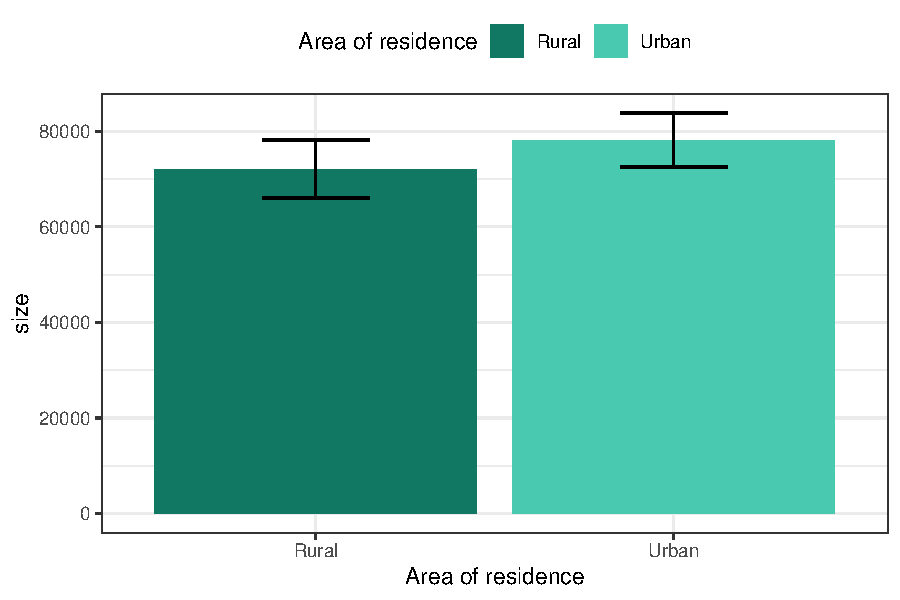
\includegraphics[width=0.7\linewidth,height=\textheight,keepaspectratio]{chapters/../figures/fig-bar-zone-1.pdf}

}

\caption{\label{fig-bar-zone}Estimación del tamaño poblacional por zona
geográfica}

\end{figure}%

El código comienza estimando, para cada categoría de la variable
\texttt{Zone}, el tamaño poblacional mediante \texttt{survey\_total()},
teniendo en cuenta el diseño muestral complejo. Además de la estimación
puntual, se solicitan el error estándar y los límites del intervalo de
confianza mediante \texttt{vartype\ =\ c("se",\ "ci")}, cuyos resultados
se almacenan en el objeto \texttt{zone\_size}. Posteriormente, se define
una paleta de colores específica para las zonas urbana y rural y se
construye el gráfico con \texttt{ggplot2}. En la estética del gráfico,
\texttt{size} determina la altura de cada barra, mientras que
\texttt{size\_low} y \texttt{size\_upp} establecen los límites inferior
y superior de las barras de error. La función \texttt{geom\_bar()}
representa los tamaños poblacionales estimados y
\texttt{geom\_errorbar()} añade los intervalos de confianza
correspondientes. Finalmente, \texttt{scale\_fill\_manual()} asigna los
colores definidos previamente, \texttt{theme\_bw()} aplica un formato
visual limpio y \texttt{theme(legend.position\ =\ "top")} ubica la
leyenda en la parte superior del gráfico.

El procedimiento anterior puede extenderse naturalmente a variables con
más de dos categorías. En estos casos, el gráfico de barras facilita la
comparación simultánea de las estimaciones correspondientes a cada
categoría y, al incorporar sus intervalos de confianza, permite apreciar
también la precisión asociada a cada una de ellas. A modo de ejemplo, a
continuación se presenta la distribución estimada de la población según
su condición de pobreza; los resultados gráficos se muestran en la
figura~\ref{fig-bar-poverty}.

\begin{Shaded}
\begin{Highlighting}[]
\NormalTok{poverty\_size }\OtherTok{\textless{}{-}} 
\NormalTok{  survey\_design }\SpecialCharTok{\%\textgreater{}\%}
  \FunctionTok{group\_by}\NormalTok{(Poverty) }\SpecialCharTok{\%\textgreater{}\%}
  \FunctionTok{summarise}\NormalTok{(}
    \AttributeTok{size =} \FunctionTok{survey\_total}\NormalTok{(}\AttributeTok{vartype =} \FunctionTok{c}\NormalTok{(}\StringTok{"se"}\NormalTok{, }\StringTok{"ci"}\NormalTok{))}
\NormalTok{  )}

\FunctionTok{ggplot}\NormalTok{(}
  \AttributeTok{data =}\NormalTok{ poverty\_size,}
  \FunctionTok{aes}\NormalTok{(}
    \AttributeTok{x =}\NormalTok{ Poverty,}
    \AttributeTok{y =}\NormalTok{ size,}
    \AttributeTok{ymax =}\NormalTok{ size\_upp,}
    \AttributeTok{ymin =}\NormalTok{ size\_low,}
    \AttributeTok{fill =}\NormalTok{ Poverty}
\NormalTok{  )}
\NormalTok{) }\SpecialCharTok{+}
  \FunctionTok{geom\_bar}\NormalTok{(}\AttributeTok{stat =} \StringTok{"identity"}\NormalTok{, }\AttributeTok{position =} \StringTok{"dodge"}\NormalTok{) }\SpecialCharTok{+}
  \FunctionTok{geom\_errorbar}\NormalTok{(}
    \AttributeTok{position =} \FunctionTok{position\_dodge}\NormalTok{(}\AttributeTok{width =} \FloatTok{0.9}\NormalTok{),}
    \AttributeTok{width =} \FloatTok{0.3}
\NormalTok{  ) }\SpecialCharTok{+}
  \FunctionTok{theme\_bw}\NormalTok{() }\SpecialCharTok{+}
  \FunctionTok{theme}\NormalTok{(}\AttributeTok{legend.position =} \StringTok{"top"}\NormalTok{)}
\end{Highlighting}
\end{Shaded}

\begin{figure}[H]

\centering{

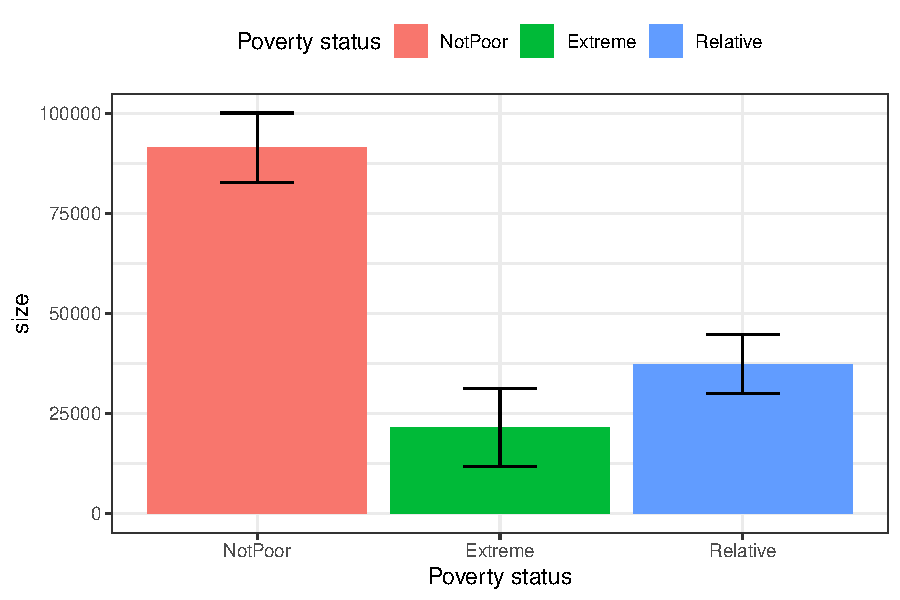
\includegraphics[width=0.7\linewidth,height=\textheight,keepaspectratio]{chapters/../figures/fig-bar-poverty-1.pdf}

}

\caption{\label{fig-bar-poverty}Estimación del número de personas según
condición de pobreza}

\end{figure}%

Una de las ventajas de los gráficos de barras es que pueden extenderse
fácilmente al análisis conjunto de dos variables categóricas. En este
contexto, permiten comparar las estimaciones correspondientes a las
distintas combinaciones de categorías y apreciar de manera visual las
diferencias entre grupos. A modo de ejemplo, se presenta la estimación
del número de personas según su condición de pobreza y estado de
ocupación, cuyos resultados se muestran en la
figura~\ref{fig-bar-employment-poverty}, obtenida con el siguiente
código computacional.

\begin{Shaded}
\begin{Highlighting}[]
\NormalTok{employment\_poverty\_size }\OtherTok{\textless{}{-}}\NormalTok{ survey\_design }\SpecialCharTok{\%\textgreater{}\%}
  \FunctionTok{filter}\NormalTok{(}\SpecialCharTok{!}\FunctionTok{is.na}\NormalTok{(Employment)) }\SpecialCharTok{\%\textgreater{}\%}
  \FunctionTok{group\_by}\NormalTok{(Employment, Poverty) }\SpecialCharTok{\%\textgreater{}\%}
  \FunctionTok{summarise}\NormalTok{(}
    \AttributeTok{size =} \FunctionTok{survey\_total}\NormalTok{(}\AttributeTok{vartype =} \FunctionTok{c}\NormalTok{(}\StringTok{"se"}\NormalTok{, }\StringTok{"ci"}\NormalTok{))}
\NormalTok{  )}

\FunctionTok{ggplot}\NormalTok{(}
\NormalTok{  employment\_poverty\_size,}
  \FunctionTok{aes}\NormalTok{(}
    \AttributeTok{x =}\NormalTok{ Poverty,}
    \AttributeTok{y =}\NormalTok{ size,}
    \AttributeTok{fill =}\NormalTok{ Employment,}
    \AttributeTok{ymin =}\NormalTok{ size\_low,}
    \AttributeTok{ymax =}\NormalTok{ size\_upp}
\NormalTok{  )}
\NormalTok{) }\SpecialCharTok{+}
  \FunctionTok{geom\_col}\NormalTok{(}\AttributeTok{position =} \FunctionTok{position\_dodge}\NormalTok{(}\AttributeTok{width =} \FloatTok{0.9}\NormalTok{)) }\SpecialCharTok{+}
  \FunctionTok{geom\_errorbar}\NormalTok{(}
    \AttributeTok{position =} \FunctionTok{position\_dodge}\NormalTok{(}\AttributeTok{width =} \FloatTok{0.9}\NormalTok{),}
    \AttributeTok{width =} \FloatTok{0.3}
\NormalTok{  ) }\SpecialCharTok{+}
  \FunctionTok{labs}\NormalTok{(}
    \AttributeTok{x =} \StringTok{"Condición de pobreza"}\NormalTok{,}
    \AttributeTok{y =} \StringTok{"Personas estimadas"}\NormalTok{,}
    \AttributeTok{fill =} \StringTok{"Condición de actividad"}
\NormalTok{  ) }\SpecialCharTok{+}
  \FunctionTok{theme\_bw}\NormalTok{() }\SpecialCharTok{+}
  \FunctionTok{theme}\NormalTok{(}\AttributeTok{legend.position =} \StringTok{"top"}\NormalTok{)}
\end{Highlighting}
\end{Shaded}

\begin{figure}[H]

\centering{

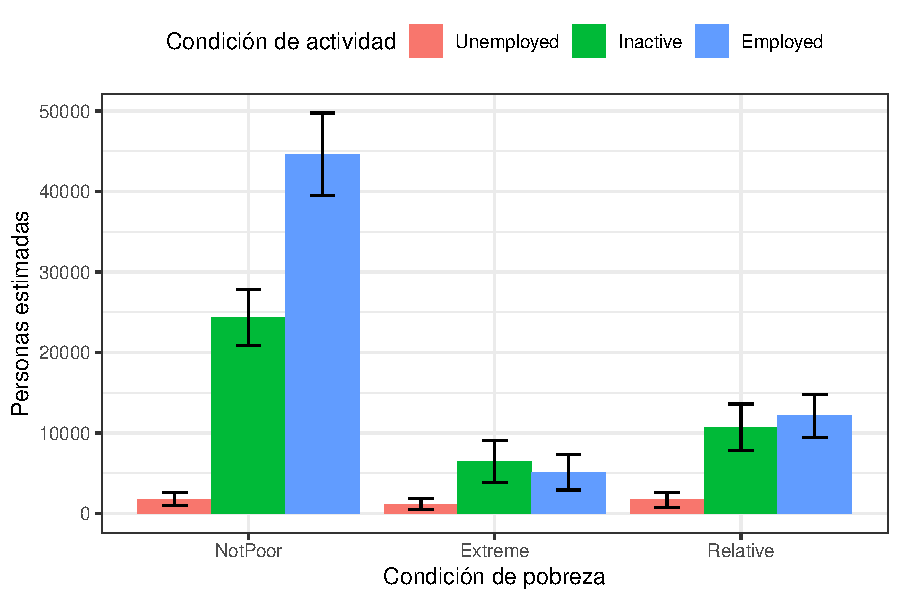
\includegraphics[width=0.8\linewidth,height=\textheight,keepaspectratio]{chapters/../figures/fig-bar-employment-poverty-1.pdf}

}

\caption{\label{fig-bar-employment-poverty}Estimación del número de
personas por estado de ocupación y situación de pobreza}

\end{figure}%

El gráfico usa las categorías originales de \texttt{Employment} y
excluye sus faltantes: no confunde inactividad con ocupación ni asigna a
los faltantes una condición laboral no observada.

Este tipo de análisis gráfico resulta especialmente útil para examinar
posibles intersecciones de vulnerabilidad, ya que permite representar
simultáneamente dos o más características de la población y comparar los
resultados entre distintos grupos. Además de mostrar conteos o tamaños
poblacionales estimados, los gráficos de barras pueden emplearse para
representar proporciones, junto con sus correspondientes medidas de
precisión. A modo de ejemplo, se presenta la proporción estimada de
hombres en condición de pobreza según zona de residencia, incorporando
los intervalos de confianza asociados a cada estimación. Se muestran las
tres categorías de pobreza dentro de cada zona de la población
masculina. Los resultados se muestran en la
figura~\ref{fig-bar-proportion-zone-male}, obtenida con el siguiente
código computacional.

\begin{Shaded}
\begin{Highlighting}[]
\NormalTok{male\_zone\_poverty\_proportion }\OtherTok{\textless{}{-}} 
\NormalTok{  male\_subset }\SpecialCharTok{\%\textgreater{}\%}
  \FunctionTok{group\_by}\NormalTok{(Zone, Poverty) }\SpecialCharTok{\%\textgreater{}\%}
  \FunctionTok{summarise}\NormalTok{(}
    \AttributeTok{proportion =} \FunctionTok{survey\_prop}\NormalTok{(}
      \AttributeTok{vartype =} \FunctionTok{c}\NormalTok{(}\StringTok{"se"}\NormalTok{, }\StringTok{"ci"}\NormalTok{),}
      \AttributeTok{proportion =} \ConstantTok{TRUE}\NormalTok{,}
      \AttributeTok{prop\_method =} \StringTok{"logit"}
\NormalTok{    )}
\NormalTok{  )}

\FunctionTok{ggplot}\NormalTok{(}
  \AttributeTok{data =}\NormalTok{ male\_zone\_poverty\_proportion,}
  \FunctionTok{aes}\NormalTok{(}
    \AttributeTok{x =}\NormalTok{ Poverty,}
    \AttributeTok{y =}\NormalTok{ proportion,}
    \AttributeTok{ymax =}\NormalTok{ proportion\_upp,}
    \AttributeTok{ymin =}\NormalTok{ proportion\_low,}
    \AttributeTok{fill =}\NormalTok{ Zone}
\NormalTok{  )}
\NormalTok{) }\SpecialCharTok{+}
  \FunctionTok{geom\_bar}\NormalTok{(}\AttributeTok{stat =} \StringTok{"identity"}\NormalTok{, }\AttributeTok{position =} \StringTok{"dodge"}\NormalTok{) }\SpecialCharTok{+}
  \FunctionTok{geom\_errorbar}\NormalTok{(}
    \AttributeTok{position =} \FunctionTok{position\_dodge}\NormalTok{(}\AttributeTok{width =} \FloatTok{0.9}\NormalTok{),}
    \AttributeTok{width =} \FloatTok{0.3}
\NormalTok{  ) }\SpecialCharTok{+}
  \FunctionTok{scale\_fill\_manual}\NormalTok{(}\AttributeTok{values =}\NormalTok{ zone\_colors) }\SpecialCharTok{+}
  \FunctionTok{theme\_bw}\NormalTok{() }\SpecialCharTok{+}
  \FunctionTok{theme}\NormalTok{(}\AttributeTok{legend.position =} \StringTok{"top"}\NormalTok{)}
\end{Highlighting}
\end{Shaded}

\begin{figure}[H]

\centering{

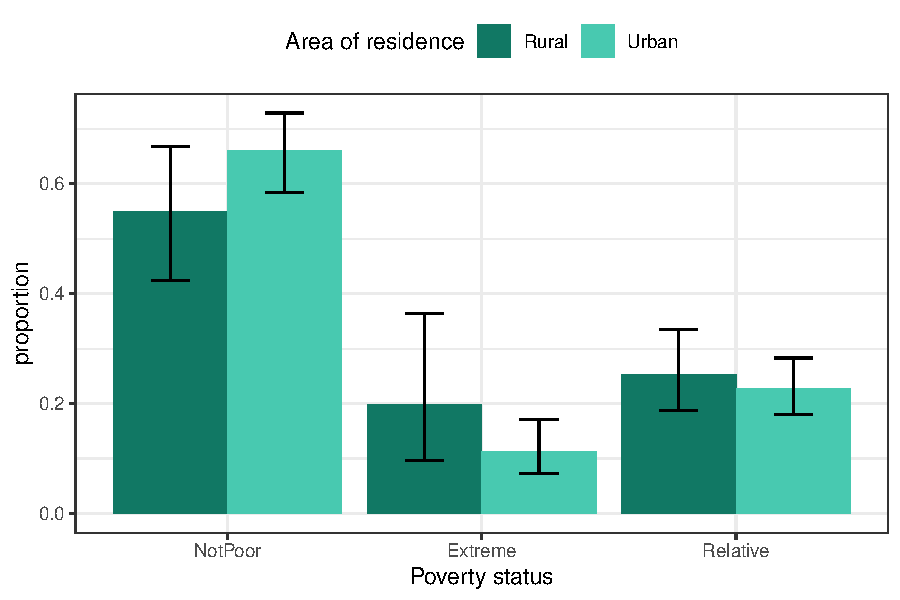
\includegraphics[width=0.7\linewidth,height=\textheight,keepaspectratio]{chapters/../figures/fig-bar-proportion-zone-male-1.pdf}

}

\caption{\label{fig-bar-proportion-zone-male}Proporción de hombres en
condición de pobreza por zona geográfica}

\end{figure}%

De manera análoga, este tipo de representación puede extenderse a
niveles más detallados de desagregación geográfica. Por ejemplo, es
posible comparar, entre regiones, las proporciones de hombres pobres y
no pobres e incorporar sus correspondientes intervalos de confianza.
Esta representación permite observar la composición de la población
masculina de cada región según la condición de pobreza y evaluar la
precisión de las estimaciones. La leyenda identifica las categorías como
«No pobre» y «Pobre»; el mapa posterior selecciona únicamente la
categoría \texttt{poor\ ==\ 1}. Los resultados se presentan en la
figura~\ref{fig-bar-proportion-region-male}, obtenida con el siguiente
código computacional.

\begin{Shaded}
\begin{Highlighting}[]
\NormalTok{male\_region\_poverty\_proportion }\OtherTok{\textless{}{-}} 
\NormalTok{  male\_subset }\SpecialCharTok{\%\textgreater{}\%}
  \FunctionTok{group\_by}\NormalTok{(Region, poor) }\SpecialCharTok{\%\textgreater{}\%}
  \FunctionTok{summarise}\NormalTok{(}
    \AttributeTok{proportion =} \FunctionTok{survey\_prop}\NormalTok{(}
      \AttributeTok{vartype =} \FunctionTok{c}\NormalTok{(}\StringTok{"se"}\NormalTok{, }\StringTok{"ci"}\NormalTok{),}
      \AttributeTok{proportion =} \ConstantTok{TRUE}\NormalTok{,}
      \AttributeTok{prop\_method =} \StringTok{"logit"}
\NormalTok{    )}
\NormalTok{  ) }\SpecialCharTok{\%\textgreater{}\%}
  \FunctionTok{data.frame}\NormalTok{()}

\FunctionTok{ggplot}\NormalTok{(}
  \AttributeTok{data =}\NormalTok{ male\_region\_poverty\_proportion,}
  \FunctionTok{aes}\NormalTok{(}
    \AttributeTok{x =}\NormalTok{ Region,}
    \AttributeTok{y =}\NormalTok{ proportion,}
    \AttributeTok{ymax =}\NormalTok{ proportion\_upp,}
    \AttributeTok{ymin =}\NormalTok{ proportion\_low,}
    \AttributeTok{fill =} \FunctionTok{factor}\NormalTok{(}
\NormalTok{      poor,}
      \AttributeTok{levels =} \FunctionTok{c}\NormalTok{(}\DecValTok{0}\NormalTok{, }\DecValTok{1}\NormalTok{),}
      \AttributeTok{labels =} \FunctionTok{c}\NormalTok{(}\StringTok{"No pobre"}\NormalTok{, }\StringTok{"Pobre"}\NormalTok{)}
\NormalTok{    )}
\NormalTok{  )}
\NormalTok{) }\SpecialCharTok{+}
  \FunctionTok{geom\_bar}\NormalTok{(}\AttributeTok{stat =} \StringTok{"identity"}\NormalTok{, }\AttributeTok{position =} \StringTok{"dodge"}\NormalTok{) }\SpecialCharTok{+}
  \FunctionTok{geom\_errorbar}\NormalTok{(}
    \AttributeTok{position =} \FunctionTok{position\_dodge}\NormalTok{(}\AttributeTok{width =} \FloatTok{0.9}\NormalTok{),}
    \AttributeTok{width =} \FloatTok{0.3}
\NormalTok{  ) }\SpecialCharTok{+}
  \FunctionTok{scale\_fill\_discrete}\NormalTok{(}\AttributeTok{name =} \StringTok{"Condición de pobreza"}\NormalTok{) }\SpecialCharTok{+}
  \FunctionTok{theme\_bw}\NormalTok{() }\SpecialCharTok{+}
  \FunctionTok{theme}\NormalTok{(}\AttributeTok{legend.position =} \StringTok{"top"}\NormalTok{)}
\end{Highlighting}
\end{Shaded}

\begin{figure}[H]

\centering{

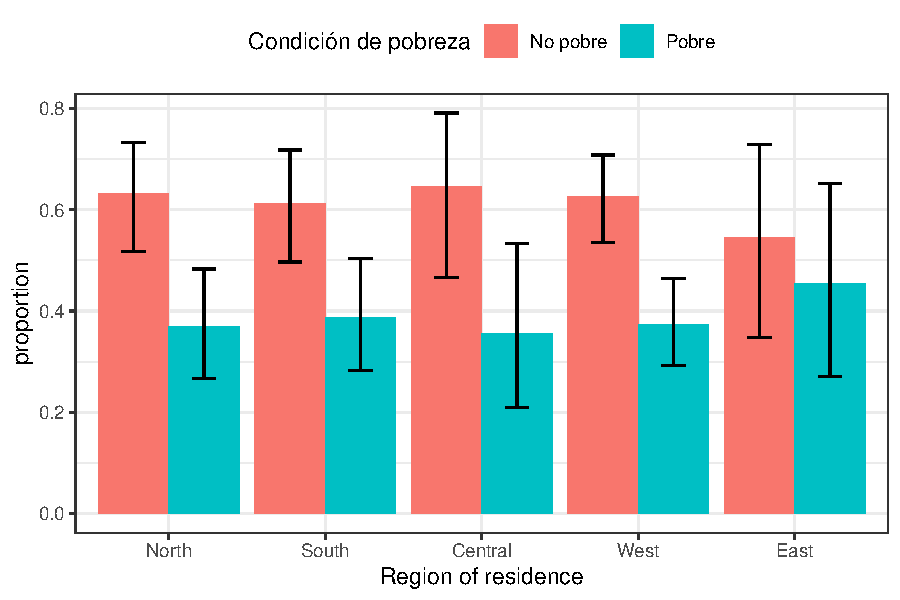
\includegraphics[width=0.75\linewidth,height=\textheight,keepaspectratio]{chapters/../figures/fig-bar-proportion-region-male-1.pdf}

}

\caption{\label{fig-bar-proportion-region-male}Proporciones de hombres
pobres y no pobres por región}

\end{figure}%

Otra forma de representar los tamaños poblacionales es la pirámide por
edad y sexo de la figura~\ref{fig-pyramid-population}, obtenida con el
siguiente código computacional. Se utilizan las estimaciones y los
intervalos de confianza de la tabla~\ref{tbl-tamano-edad-sexo},
almacenados en \texttt{age\_sex\_population\_size}. Los hombres se
sitúan a la izquierda, en azul, y las mujeres a la derecha, en rosa; los
grupos de menor edad aparecen en la base. La longitud de cada barra
representa el número estimado de personas y las líneas negras muestran
sus intervalos de confianza del 95 \%.

\begin{Shaded}
\begin{Highlighting}[]
\FunctionTok{ggplot}\NormalTok{(}
\NormalTok{  age\_sex\_population\_size,}
  \FunctionTok{aes}\NormalTok{(}
    \AttributeTok{x =} \FunctionTok{factor}\NormalTok{(CatAge, }\AttributeTok{levels =} \FunctionTok{unique}\NormalTok{(CatAge)),}
    \AttributeTok{y =} \FunctionTok{if\_else}\NormalTok{(Sex }\SpecialCharTok{==} \StringTok{"Male"}\NormalTok{, }\SpecialCharTok{{-}}\NormalTok{size, size),}
    \AttributeTok{ymin =} \FunctionTok{if\_else}\NormalTok{(Sex }\SpecialCharTok{==} \StringTok{"Male"}\NormalTok{, }\SpecialCharTok{{-}}\NormalTok{size\_upp, size\_low),}
    \AttributeTok{ymax =} \FunctionTok{if\_else}\NormalTok{(Sex }\SpecialCharTok{==} \StringTok{"Male"}\NormalTok{, }\SpecialCharTok{{-}}\NormalTok{size\_low, size\_upp),}
    \AttributeTok{fill =}\NormalTok{ Sex}
\NormalTok{  )}
\NormalTok{) }\SpecialCharTok{+}
  \FunctionTok{geom\_col}\NormalTok{(}\AttributeTok{width =} \FloatTok{0.8}\NormalTok{) }\SpecialCharTok{+}
  \FunctionTok{geom\_errorbar}\NormalTok{(}\AttributeTok{width =} \FloatTok{0.2}\NormalTok{) }\SpecialCharTok{+}
  \FunctionTok{geom\_hline}\NormalTok{(}\AttributeTok{yintercept =} \DecValTok{0}\NormalTok{) }\SpecialCharTok{+}
  \FunctionTok{coord\_flip}\NormalTok{() }\SpecialCharTok{+}
  \FunctionTok{scale\_y\_continuous}\NormalTok{(}
    \AttributeTok{limits =} \ControlFlowTok{function}\NormalTok{(x) }\FunctionTok{c}\NormalTok{(}\SpecialCharTok{{-}}\FunctionTok{max}\NormalTok{(}\FunctionTok{abs}\NormalTok{(x)), }\FunctionTok{max}\NormalTok{(}\FunctionTok{abs}\NormalTok{(x))),}
    \AttributeTok{labels =} \ControlFlowTok{function}\NormalTok{(x) }\FunctionTok{format}\NormalTok{(}
      \FunctionTok{abs}\NormalTok{(x),}
      \AttributeTok{big.mark =} \StringTok{"."}\NormalTok{,}
      \AttributeTok{decimal.mark =} \StringTok{","}
\NormalTok{    )}
\NormalTok{  ) }\SpecialCharTok{+}
  \FunctionTok{scale\_fill\_manual}\NormalTok{(}
    \AttributeTok{values =} \FunctionTok{c}\NormalTok{(}\AttributeTok{Male =} \StringTok{"\#4A90D9"}\NormalTok{, }\AttributeTok{Female =} \StringTok{"\#E78AB5"}\NormalTok{),}
    \AttributeTok{breaks =} \FunctionTok{c}\NormalTok{(}\StringTok{"Male"}\NormalTok{, }\StringTok{"Female"}\NormalTok{),}
    \AttributeTok{labels =} \FunctionTok{c}\NormalTok{(}\StringTok{"Hombres"}\NormalTok{, }\StringTok{"Mujeres"}\NormalTok{)}
\NormalTok{  ) }\SpecialCharTok{+}
  \FunctionTok{labs}\NormalTok{(}
    \AttributeTok{x =} \StringTok{"Grupo de edad (años)"}\NormalTok{,}
    \AttributeTok{y =} \StringTok{"Personas"}\NormalTok{,}
    \AttributeTok{fill =} \ConstantTok{NULL}
\NormalTok{  ) }\SpecialCharTok{+}
  \FunctionTok{theme\_bw}\NormalTok{() }\SpecialCharTok{+}
  \FunctionTok{theme}\NormalTok{(}\AttributeTok{legend.position =} \StringTok{"top"}\NormalTok{)}
\end{Highlighting}
\end{Shaded}

\begin{figure}[H]

\centering{

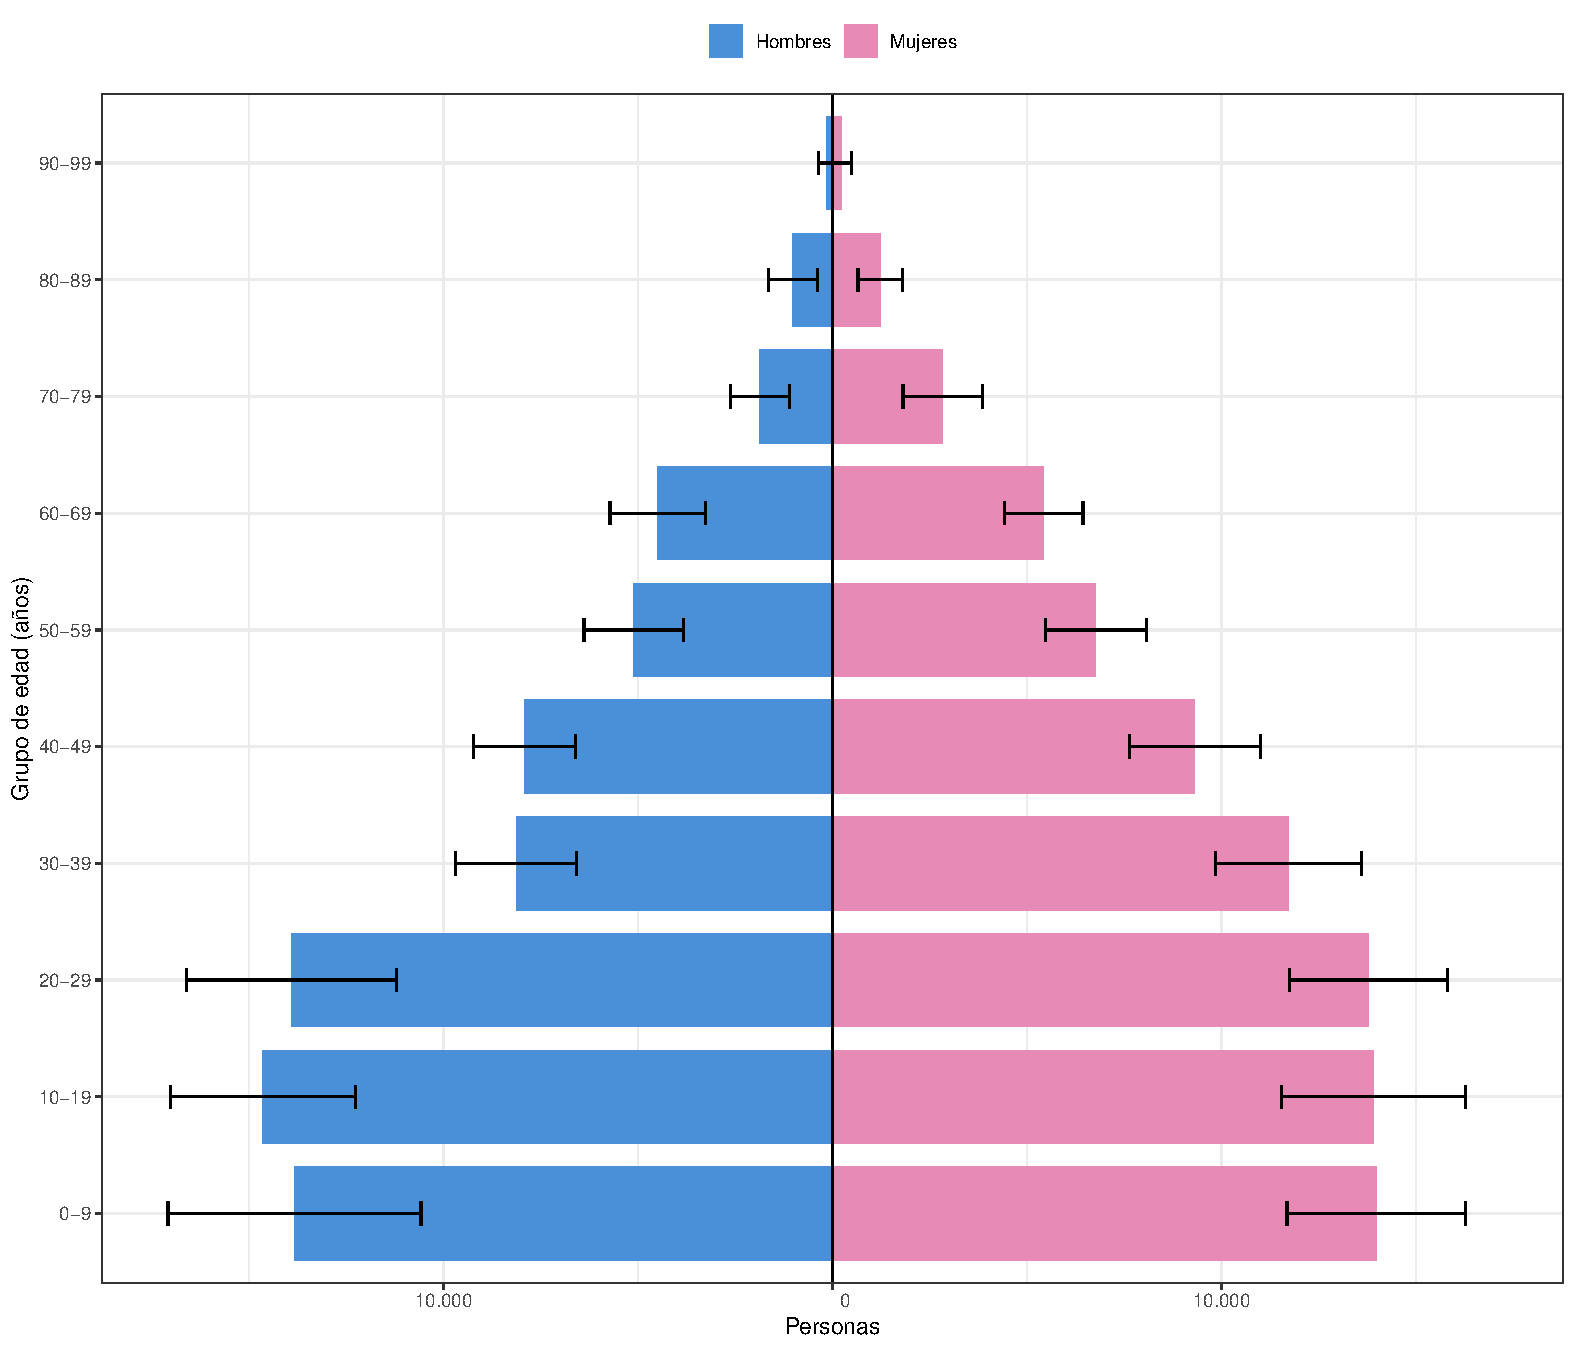
\includegraphics[width=1\linewidth,height=\textheight,keepaspectratio]{chapters/../figures/fig-pyramid-population-1.pdf}

}

\caption{\label{fig-pyramid-population}Pirámide de población estimada
por edad y sexo con intervalos de confianza del 95 \%}

\end{figure}%

En el código, \texttt{ggplot()} utiliza directamente el objeto
\texttt{age\_sex\_population\_size}. Dentro de \texttt{aes()},
\texttt{factor(CatAge,\ levels\ =\ unique(CatAge))} conserva el orden de
los grupos de edad del objeto, previamente ordenado, mientras que
\texttt{if\_else()} determina la posición de las barras y de sus
intervalos según el sexo. Los tamaños de los hombres se multiplican por
menos uno únicamente para dibujarlos a la izquierda; no representan
poblaciones negativas. Al invertir el signo, también se intercambian los
extremos del intervalo: el inferior pasa a ser \texttt{-size\_upp} y el
superior, \texttt{-size\_low}. \texttt{geom\_col()} utiliza las
estimaciones ya calculadas y equivale a
\texttt{geom\_bar(stat\ =\ "identity")}; \texttt{geom\_errorbar()}
incorpora sus intervalos. \texttt{coord\_flip()} orienta las barras
horizontalmente, \texttt{scale\_y\_continuous()} establece una escala
simétrica con valores absolutos a ambos lados. Finalmente,
\texttt{scale\_fill\_manual()} asigna los colores y las etiquetas de la
leyenda, y \texttt{theme\_bw()} conserva el estilo de los gráficos
anteriores.

La pirámide muestra que el grupo de 10-19 años reúne el mayor tamaño
poblacional estimado. En ese grupo se estiman aproximadamente 13.909
mujeres y 14.645 hombres. Las barras de error permiten apreciar la
incertidumbre de cada tamaño estimado, pero la comparación visual de sus
intervalos no sustituye una prueba de contraste entre sexos que
considere la covarianza de las estimaciones.

Las categorías de \texttt{CatAge} tienen una amplitud uniforme de diez
años, de \texttt{0-9} a \texttt{90-99}, lo que facilita comparar los
tamaños de los grupos en la pirámide. En la muestra hay observaciones de
ambos sexos en los diez grupos decenales. Las edades más avanzadas
tienen pocas observaciones y requieren especial atención a la
incertidumbre de sus estimaciones. La forma del gráfico, por sí sola, no
permite atribuir diferencias a la fecundidad, la mortalidad o la
migración.

Las estimaciones por edad y sexo también permiten construir indicadores
de la estructura demográfica de la población. Por ejemplo, la razón de
dependencia demográfica relaciona el número de personas menores de 15
años y de 65 años o más con el número de personas de 15 a 64 años. Su
estimación requiere considerar conjuntamente la incertidumbre de los
tamaños poblacionales del numerador y del denominador, así como su
covarianza. En la \hyperref[estimacion-de-razones]{sección de estimación
de razones} se desarrolla esta aplicación y se muestra cómo obtener sus
medidas de precisión incorporando el diseño muestral.

\subsection{Mapas temáticos}\label{viz-mapas}

Como explica Tennekes (\citeproc{ref-Tennekes2018tmap}{2018}), los mapas
temáticos constituyen una herramienta de visualización especialmente
útil en el análisis de encuestas de hogares, ya que permiten representar
la distribución territorial de indicadores sociales y demográficos. En
este contexto, las estimaciones calculadas en secciones anteriores
pueden proyectarse directamente sobre estas unidades geográficas,
facilitando así la identificación de patrones espaciales y desigualdades
regionales. De acuerdo con Pebesma et~al. (\citeproc{ref-sf2026}{2026}),
Tennekes (\citeproc{ref-tmap2026}{2026}) y Pebesma
(\citeproc{ref-Pebesma2018sf}{2018}), para construir este tipo de mapas
en \texttt{R} se requiere información geoespacial en formato
\emph{shapefile}, la cual contiene los polígonos asociados a cada unidad
geográfica de análisis. En este capítulo se utiliza el archivo
\texttt{shapeBigCity/BigCity.shp}, cuyas regiones corresponden a las
definidas en la base de datos \texttt{BigCity}.

El siguiente código computacional carga las librerías \texttt{sf} y
\texttt{tmap} para trabajar con la información geográfica y vincularla
con los resultados de la encuesta. La librería \texttt{sf} permite leer
y manipular objetos espaciales modernos, mientras que \texttt{tmap}
proporciona herramientas para elaborar mapas temáticos. La instrucción
\texttt{tmap\_mode("plot")} establece el modo de visualización estática
de los mapas, apropiado para documentos y reportes. Finalmente, la
función \texttt{read\_sf()} importa el archivo geográfico
\texttt{BigCity.shp}, almacenándolo en el objeto
\texttt{bigcity\_shape}, el cual contiene los polígonos correspondientes
a las regiones de análisis.

\begin{Shaded}
\begin{Highlighting}[]
\FunctionTok{library}\NormalTok{(sf)}
\FunctionTok{library}\NormalTok{(tmap)}
\FunctionTok{tmap\_mode}\NormalTok{(}\StringTok{"plot"}\NormalTok{)}
\NormalTok{bigcity\_shape }\OtherTok{\textless{}{-}} \FunctionTok{read\_sf}\NormalTok{(}\StringTok{"../data/shapeBigCity/BigCity.shp"}\NormalTok{) }\SpecialCharTok{\%\textgreater{}\%}
  \FunctionTok{mutate}\NormalTok{(}
    \AttributeTok{Region =} \FunctionTok{recode}\NormalTok{(}
\NormalTok{      Region,}
      \AttributeTok{Norte =} \StringTok{"North"}\NormalTok{,}
      \AttributeTok{Sur =} \StringTok{"South"}\NormalTok{,}
      \AttributeTok{Centro =} \StringTok{"Central"}\NormalTok{,}
      \AttributeTok{Occidente =} \StringTok{"West"}\NormalTok{,}
      \AttributeTok{Oriente =} \StringTok{"East"}
\NormalTok{    )}
\NormalTok{  )}
\end{Highlighting}
\end{Shaded}

La columna \texttt{Region} del mapa se recodifica al inglés para que sus
nombres coincidan con los de \texttt{sample.rds} y permitan unir el mapa
con las estimaciones. La recodificación se realiza en el objeto cargado
en R y conserva el archivo geográfico original. Con el \emph{shapefile}
cargado, el siguiente código computacional genera el mapa de la
figura~\ref{fig-map-regions} mediante \texttt{tm\_shape()} y
\texttt{tm\_polygons()}.

\begin{Shaded}
\begin{Highlighting}[]
\FunctionTok{tm\_shape}\NormalTok{(bigcity\_shape) }\SpecialCharTok{+}
  \FunctionTok{tm\_polygons}\NormalTok{(}\AttributeTok{col =} \StringTok{"Region"}\NormalTok{)}
\end{Highlighting}
\end{Shaded}

\begin{figure}[H]

\centering{

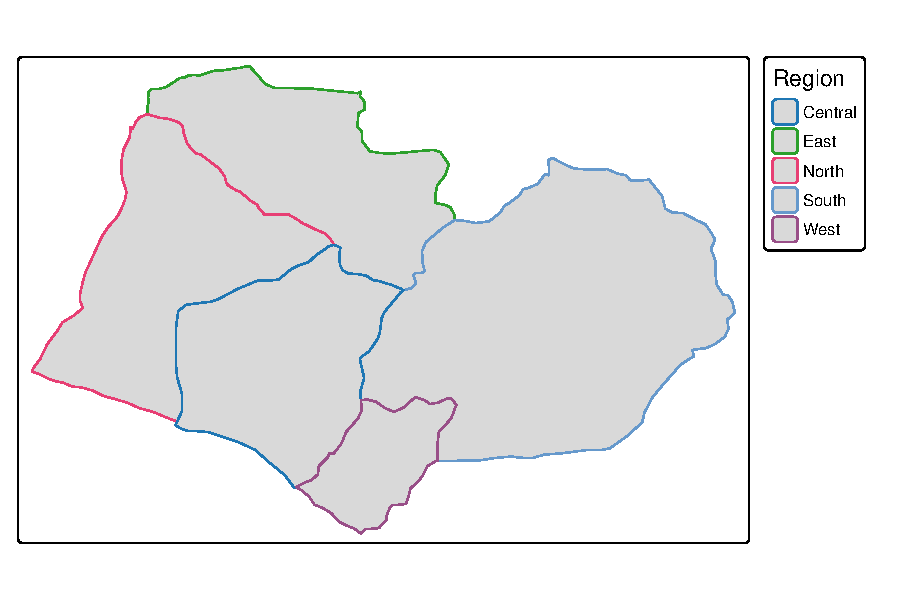
\includegraphics[width=0.7\linewidth,height=\textheight,keepaspectratio]{chapters/../figures/fig-map-regions-1.pdf}

}

\caption{\label{fig-map-regions}Mapa de regiones geográficas de BigCity}

\end{figure}%

Por ejemplo, si se desea representar geográficamente la proporción de
hombres en condición de pobreza por región, mostrada previamente en la
figura~\ref{fig-bar-proportion-region-male}, es necesario integrar las
estimaciones obtenidas con la información espacial del shapefile. En el
siguiente código computacional, el objeto
\texttt{male\_region\_poverty\_proportion}, que contiene las
proporciones estimadas para cada región, se vincula con el archivo
geográfico mediante la función \texttt{left\_join()}. Posteriormente, se
filtran únicamente las observaciones correspondientes a la categoría de
pobreza (\texttt{poor\ ==\ 1}), de manera que el mapa represente
exclusivamente la distribución espacial de la población masculina en
condición de pobreza.

\begin{Shaded}
\begin{Highlighting}[]
\NormalTok{shape\_region\_map }\OtherTok{\textless{}{-}} \FunctionTok{tm\_shape}\NormalTok{(}
\NormalTok{  bigcity\_shape }\SpecialCharTok{\%\textgreater{}\%}
    \FunctionTok{left\_join}\NormalTok{(}
\NormalTok{      male\_region\_poverty\_proportion }\SpecialCharTok{\%\textgreater{}\%}
        \FunctionTok{filter}\NormalTok{(poor }\SpecialCharTok{==} \DecValTok{1}\NormalTok{),}
      \AttributeTok{by =} \StringTok{"Region"}
\NormalTok{    )}
\NormalTok{)}
\end{Highlighting}
\end{Shaded}

Una vez construido el objeto espacial con las estimaciones de interés,
los puntos de corte de la escala de color se calculan a partir del rango
observado de las proporciones de hombres pobres. Así, los colores
permiten distinguir mejor las diferencias entre regiones cuando las
estimaciones se concentran en un tramo reducido de la escala de cero a
uno. El siguiente código computacional representa esta distribución
regional en la figura~\ref{fig-map-poverty-male}; sus colores deben
interpretarse según los intervalos indicados en la leyenda.

\begin{Shaded}
\begin{Highlighting}[]
\NormalTok{poverty\_estimates }\OtherTok{\textless{}{-}}\NormalTok{ male\_region\_poverty\_proportion }\SpecialCharTok{\%\textgreater{}\%}
  \FunctionTok{filter}\NormalTok{(poor }\SpecialCharTok{==} \DecValTok{1}\NormalTok{) }\SpecialCharTok{\%\textgreater{}\%}
  \FunctionTok{pull}\NormalTok{(proportion)}
\NormalTok{poverty\_breaks }\OtherTok{\textless{}{-}} \FunctionTok{pretty}\NormalTok{(}
  \FunctionTok{range}\NormalTok{(poverty\_estimates, }\AttributeTok{na.rm =} \ConstantTok{TRUE}\NormalTok{),}
  \AttributeTok{n =} \DecValTok{5}
\NormalTok{)}
\NormalTok{shape\_region\_map }\SpecialCharTok{+}
  \FunctionTok{tm\_polygons}\NormalTok{(}
    \AttributeTok{fill =} \StringTok{"proportion"}\NormalTok{,}
    \AttributeTok{fill.scale =} \FunctionTok{tm\_scale\_intervals}\NormalTok{(}
      \AttributeTok{breaks =}\NormalTok{ poverty\_breaks,}
      \AttributeTok{values =} \StringTok{"YlOrRd"}
\NormalTok{    ),}
    \AttributeTok{fill.legend =} \FunctionTok{tm\_legend}\NormalTok{(}
      \AttributeTok{title =} \StringTok{"Poverty proportion"}\NormalTok{,}
      \AttributeTok{na.show =} \ConstantTok{FALSE}
\NormalTok{    )}
\NormalTok{  )}
\end{Highlighting}
\end{Shaded}

\begin{figure}[H]

\centering{

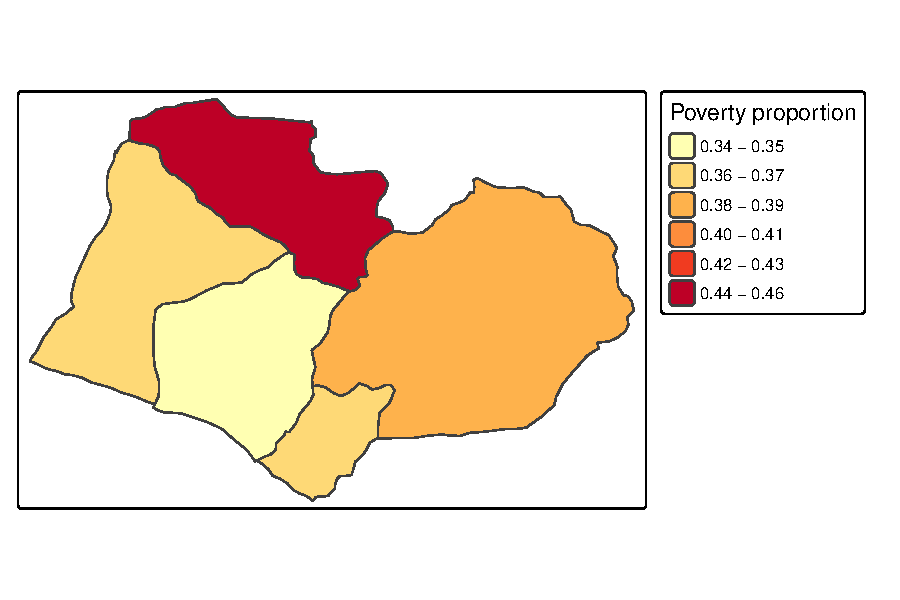
\includegraphics[width=0.7\linewidth,height=\textheight,keepaspectratio]{chapters/../figures/fig-map-poverty-male-1.pdf}

}

\caption{\label{fig-map-poverty-male}Proporción de hombres en condición
de pobreza por región}

\end{figure}%

Otro uso de los mapas en encuestas, señalado por CEPAL
(\citeproc{ref-CEPAL2023Diseno}{2023}), es la visualización de la
precisión de las estimaciones. Por ejemplo, usando el coeficiente de
variación de la proporción de pobreza por región es posible identificar
las áreas donde las estimaciones son menos confiables, como se muestra
en la figura~\ref{fig-map-cv-poverty}.

El siguiente código calcula y representa geográficamente el coeficiente
de variación de la proporción de pobreza por región. En primer lugar, se
estima la proporción de pobreza agrupando por \texttt{Region} y
\texttt{poor} y aplicando \texttt{survey\_prop()}; después se conserva
la categoría \texttt{poor\ ==\ 1}. El argumento
\texttt{vartype\ =\ "cv"} solicita el cálculo del coeficiente de
variación de cada estimación. Posteriormente, se definen los intervalos
de clasificación de la escala de color mediante el objeto
\texttt{cv\_breaks}, y las estimaciones se integran con la información
geográfica del shapefile usando \texttt{left\_join()}. Finalmente,
mediante las funciones \texttt{tm\_shape()} y \texttt{tm\_polygons()}
del paquete \texttt{tmap}, se construye el mapa que representa
espacialmente los coeficientes de variación utilizando una escala de
colores en blanco y negro y ajustando la proporción del mapa con
\texttt{tm\_layout(asp\ =\ 0)}.

\begin{Shaded}
\begin{Highlighting}[]
\NormalTok{region\_poverty\_cv }\OtherTok{\textless{}{-}}\NormalTok{ survey\_design }\SpecialCharTok{\%\textgreater{}\%}
  \FunctionTok{filter}\NormalTok{(}\SpecialCharTok{!}\FunctionTok{is.na}\NormalTok{(poor)) }\SpecialCharTok{\%\textgreater{}\%}
  \FunctionTok{group\_by}\NormalTok{(Region, poor) }\SpecialCharTok{\%\textgreater{}\%}
  \FunctionTok{summarise}\NormalTok{(}
    \AttributeTok{proportion =} \FunctionTok{survey\_prop}\NormalTok{(}
      \AttributeTok{proportion =} \ConstantTok{TRUE}\NormalTok{,}
      \AttributeTok{prop\_method =} \StringTok{"logit"}\NormalTok{,}
      \AttributeTok{vartype =} \StringTok{"cv"}
\NormalTok{    ),}
    \AttributeTok{.groups =} \StringTok{"drop"}
\NormalTok{  ) }\SpecialCharTok{\%\textgreater{}\%}
  \FunctionTok{filter}\NormalTok{(poor }\SpecialCharTok{==} \DecValTok{1}\NormalTok{) }\SpecialCharTok{\%\textgreater{}\%}
  \FunctionTok{select}\NormalTok{(}\SpecialCharTok{{-}}\NormalTok{poor)}

\NormalTok{cv\_breaks }\OtherTok{\textless{}{-}} \FunctionTok{c}\NormalTok{(}\DecValTok{0}\NormalTok{, }\FloatTok{0.1}\NormalTok{, }\FloatTok{0.2}\NormalTok{, }\ConstantTok{Inf}\NormalTok{)}
\NormalTok{shape\_cv\_map }\OtherTok{\textless{}{-}} \FunctionTok{tm\_shape}\NormalTok{(}
\NormalTok{  bigcity\_shape }\SpecialCharTok{\%\textgreater{}\%}
    \FunctionTok{left\_join}\NormalTok{(region\_poverty\_cv, }\AttributeTok{by =} \StringTok{"Region"}\NormalTok{)}
\NormalTok{)}

\NormalTok{shape\_cv\_map }\SpecialCharTok{+}
  \FunctionTok{tm\_polygons}\NormalTok{(}
    \AttributeTok{fill =} \StringTok{"proportion\_cv"}\NormalTok{,}
    \AttributeTok{fill.scale =} \FunctionTok{tm\_scale\_intervals}\NormalTok{(}
      \AttributeTok{breaks =}\NormalTok{ cv\_breaks,}
      \AttributeTok{values =} \FunctionTok{c}\NormalTok{(}\StringTok{"\#F2F2F2"}\NormalTok{, }\StringTok{"\#8C8C8C"}\NormalTok{, }\StringTok{"\#1A1A1A"}\NormalTok{)}
\NormalTok{    ),}
    \AttributeTok{fill.legend =} \FunctionTok{tm\_legend}\NormalTok{(}
      \AttributeTok{title =} \StringTok{"CV de la proporción"}\NormalTok{,}
      \AttributeTok{na.show =} \ConstantTok{FALSE}
\NormalTok{    )}
\NormalTok{  ) }\SpecialCharTok{+}
  \FunctionTok{tm\_layout}\NormalTok{(}\AttributeTok{asp =} \DecValTok{0}\NormalTok{)}
\end{Highlighting}
\end{Shaded}

\begin{figure}[H]

\centering{

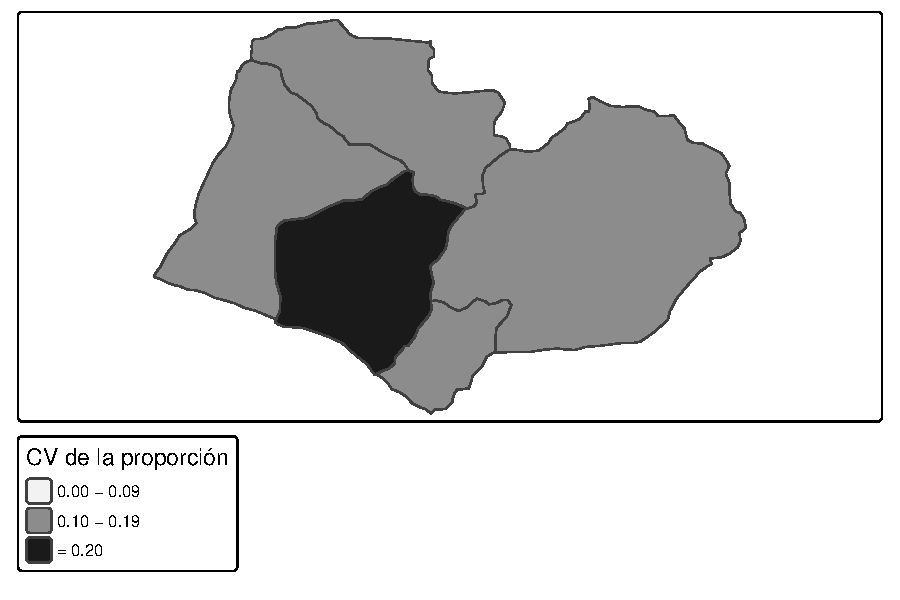
\includegraphics[width=0.7\linewidth,height=\textheight,keepaspectratio]{chapters/../figures/fig-map-cv-poverty-1.pdf}

}

\caption{\label{fig-map-cv-poverty}Coeficiente de variación de la
proporción de pobreza por región}

\end{figure}%

Los polígonos con tonos más oscuros corresponden a regiones donde la
proporción estimada presenta mayor variabilidad relativa. El CV se
expresa como razón, de modo que 0,1 equivale al 10 \%; no representa el
error estándar en \%. Un coeficiente de variación elevado indica menor
precisión relativa, pero no permite atribuirla únicamente a un tamaño
muestral insuficiente, pues también puede reflejar la ponderación y
otras características del diseño.

De acuerdo con Prener et~al. (\citeproc{ref-biscale2025}{2025}) y Wilke
(\citeproc{ref-cowplot2025}{2025}), cuando se desea representar
simultáneamente dos variables (por ejemplo, la proporción de pobreza y
su coeficiente de variación) es posible construir un mapa bivariante
utilizando \texttt{ggplot2} junto con los paquetes \texttt{biscale} y
\texttt{cowplot}. Este tipo de visualización permite identificar
regiones con alta pobreza y alta incertidumbre en la estimación de forma
conjunta, como se presenta en la figura~\ref{fig-map-bivariate}. El
siguiente código estima la proporción de mujeres en condición de pobreza
en zonas rurales para cada región, incorporando además el cálculo del
coeficiente de variación de las estimaciones, generando una fila por
región. El denominador es la población femenina rural de cada región; el
CV expresa precisión relativa y no incertidumbre absoluta.

\begin{Shaded}
\begin{Highlighting}[]
\NormalTok{region\_sex\_poverty\_proportion }\OtherTok{\textless{}{-}}\NormalTok{ survey\_design }\SpecialCharTok{\%\textgreater{}\%}
  \FunctionTok{filter}\NormalTok{(Zone }\SpecialCharTok{==} \StringTok{"Rural"}\NormalTok{, Sex }\SpecialCharTok{==} \StringTok{"Female"}\NormalTok{) }\SpecialCharTok{\%\textgreater{}\%}
  \FunctionTok{filter}\NormalTok{(}\SpecialCharTok{!}\FunctionTok{is.na}\NormalTok{(poor)) }\SpecialCharTok{\%\textgreater{}\%}
  \FunctionTok{group\_by}\NormalTok{(Region, poor) }\SpecialCharTok{\%\textgreater{}\%}
  \FunctionTok{summarise}\NormalTok{(}
    \AttributeTok{proportion =} \FunctionTok{survey\_prop}\NormalTok{(}
      \AttributeTok{proportion =} \ConstantTok{TRUE}\NormalTok{,}
      \AttributeTok{prop\_method =} \StringTok{"logit"}\NormalTok{,}
      \AttributeTok{vartype =} \StringTok{"cv"}
\NormalTok{    ),}
    \AttributeTok{.groups =} \StringTok{"drop"}
\NormalTok{  ) }\SpecialCharTok{\%\textgreater{}\%}
  \FunctionTok{filter}\NormalTok{(poor }\SpecialCharTok{==} \DecValTok{1}\NormalTok{) }\SpecialCharTok{\%\textgreater{}\%}
  \FunctionTok{select}\NormalTok{(}\SpecialCharTok{{-}}\NormalTok{poor)}
\end{Highlighting}
\end{Shaded}

El siguiente código construye un mapa bivariado que permite visualizar
simultáneamente la proporción de pobreza femenina rural y el coeficiente
de variación asociado a dicha estimación por región. En primer lugar, se
integran las estimaciones contenidas en
\texttt{region\_sex\_poverty\_proportion} con la información geográfica
del shapefile mediante \texttt{left\_join()}. Posteriormente, la función
\texttt{bi\_class()} del paquete \texttt{biscale} clasifica
conjuntamente las variables \texttt{proportion} y
\texttt{proportion\_cv} en una cuadrícula de \((3 \times 3)\) categorías
(\texttt{dim\ =\ 3}), empleando el método de clasificación de Fisher
(\texttt{style\ =\ "fisher"}). Luego, con \texttt{ggplot2} y
\texttt{geom\_sf()}, se genera el mapa temático utilizando colores
bivariados definidos por \texttt{bi\_scale\_fill()}, mientras que
\texttt{bi\_theme()} aplica un estilo minimalista y se elimina la
leyenda predeterminada.

A continuación, la función \texttt{bi\_legend()} crea una leyenda
especializada que permite interpretar simultáneamente ambas dimensiones
del mapa: el coeficiente de variación y la pobreza femenina rural.
Finalmente, mediante las funciones \texttt{ggdraw()} y
\texttt{draw\_plot()} del paquete \texttt{cowplot}, se combinan el mapa
y la leyenda en una única visualización.

\begin{Shaded}
\begin{Highlighting}[]
\FunctionTok{library}\NormalTok{(biscale)}
\FunctionTok{library}\NormalTok{(cowplot)}

\NormalTok{bivariate\_shape }\OtherTok{\textless{}{-}}\NormalTok{ bigcity\_shape }\SpecialCharTok{\%\textgreater{}\%}
  \FunctionTok{left\_join}\NormalTok{(region\_sex\_poverty\_proportion, }\AttributeTok{by =} \StringTok{"Region"}\NormalTok{)}

\NormalTok{k }\OtherTok{\textless{}{-}} \DecValTok{3}
\NormalTok{bivariate\_palette }\OtherTok{\textless{}{-}} \StringTok{"DkViolet"}
\NormalTok{bivariate\_data }\OtherTok{\textless{}{-}} \FunctionTok{bi\_class}\NormalTok{(}
\NormalTok{  bivariate\_shape,}
  \AttributeTok{y =}\NormalTok{ proportion,}
  \AttributeTok{x =}\NormalTok{ proportion\_cv,}
  \AttributeTok{dim =}\NormalTok{ k,}
  \AttributeTok{style =} \StringTok{"fisher"}
\NormalTok{)}

\NormalTok{bivariate\_map }\OtherTok{\textless{}{-}} \FunctionTok{ggplot}\NormalTok{() }\SpecialCharTok{+}
  \FunctionTok{geom\_sf}\NormalTok{(}
    \AttributeTok{data =}\NormalTok{ bivariate\_data,}
    \FunctionTok{aes}\NormalTok{(}\AttributeTok{fill =}\NormalTok{ bi\_class, }\AttributeTok{geometry =}\NormalTok{ geometry),}
    \AttributeTok{colour =} \StringTok{"white"}\NormalTok{,}
    \AttributeTok{size =} \FloatTok{0.1}
\NormalTok{  ) }\SpecialCharTok{+}
  \FunctionTok{bi\_scale\_fill}\NormalTok{(}\AttributeTok{pal =}\NormalTok{ bivariate\_palette, }\AttributeTok{dim =}\NormalTok{ k) }\SpecialCharTok{+}
  \FunctionTok{bi\_theme}\NormalTok{() }\SpecialCharTok{+}
  \FunctionTok{theme}\NormalTok{(}\AttributeTok{legend.position =} \StringTok{"none"}\NormalTok{)}

\NormalTok{bivariate\_legend }\OtherTok{\textless{}{-}} \FunctionTok{bi\_legend}\NormalTok{(}
  \AttributeTok{pal =}\NormalTok{ bivariate\_palette,}
  \AttributeTok{dim =}\NormalTok{ k,}
  \AttributeTok{xlab =} \StringTok{"Coefficient of variation"}\NormalTok{,}
  \AttributeTok{ylab =} \StringTok{"Rural female poverty"}\NormalTok{,}
  \AttributeTok{size =} \DecValTok{6}
\NormalTok{)}

\FunctionTok{ggdraw}\NormalTok{() }\SpecialCharTok{+}
  \FunctionTok{draw\_plot}\NormalTok{(bivariate\_map, }\FloatTok{0.02}\NormalTok{, }\FloatTok{0.04}\NormalTok{, }\FloatTok{0.68}\NormalTok{, }\FloatTok{0.9}\NormalTok{) }\SpecialCharTok{+}
  \FunctionTok{draw\_plot}\NormalTok{(bivariate\_legend, }\FloatTok{0.67}\NormalTok{, }\FloatTok{0.25}\NormalTok{, }\FloatTok{0.3}\NormalTok{, }\FloatTok{0.38}\NormalTok{)}
\end{Highlighting}
\end{Shaded}

\begin{figure}[H]

\centering{

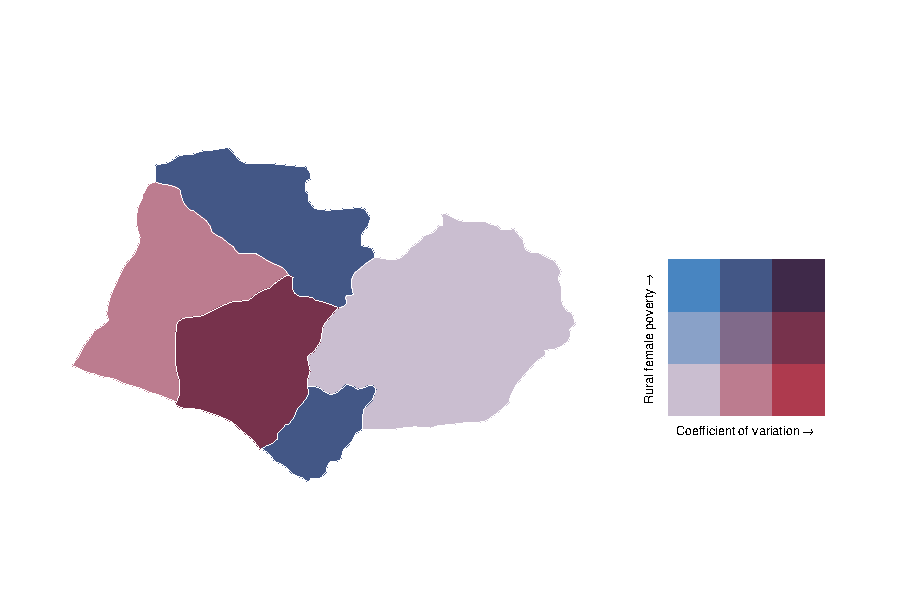
\includegraphics[width=0.8\linewidth,height=\textheight,keepaspectratio]{chapters/../figures/fig-map-bivariate-1.pdf}

}

\caption{\label{fig-map-bivariate}Mapa bivariante: proporción de pobreza
femenina rural y su coeficiente de variación por región}

\end{figure}%

En este mapa, cada celda de la leyenda combina un tono de la proporción
de pobreza (eje vertical) con un tono del coeficiente de variación (eje
horizontal), permitiendo identificar simultáneamente regiones con alta
pobreza y alta incertidumbre en la estimación. Este tipo de
representación puede ayudar a priorizar una evaluación del diseño y de
la precisión en zonas geográficas específicas; por sí solo, sin embargo,
no determina automáticamente que deba ampliarse el tamaño muestral.

Al desagregar los resultados por territorio y características
sociodemográficas, algunas estimaciones directas pueden presentar una
precisión limitada. El siguiente código computacional ilustra esta
situación al estimar la proporción de pobreza entre las mujeres rurales
de 15 a 29 años de cada región y resumir su precisión, incorporando los
factores de expansión, los estratos y las UPM del diseño muestral.

\begin{Shaded}
\begin{Highlighting}[]
\NormalTok{rural\_young\_women }\OtherTok{\textless{}{-}}\NormalTok{ survey\_design }\SpecialCharTok{\%\textgreater{}\%}
  \FunctionTok{filter}\NormalTok{(}
\NormalTok{    Sex }\SpecialCharTok{==} \StringTok{"Female"}\NormalTok{,}
\NormalTok{    Zone }\SpecialCharTok{==} \StringTok{"Rural"}\NormalTok{,}
\NormalTok{    Age }\SpecialCharTok{\textgreater{}=} \DecValTok{15}\NormalTok{,}
\NormalTok{    Age }\SpecialCharTok{\textless{}=} \DecValTok{29}\NormalTok{,}
    \SpecialCharTok{!}\FunctionTok{is.na}\NormalTok{(poor)}
\NormalTok{  )}

\NormalTok{rural\_young\_women\_sizes }\OtherTok{\textless{}{-}}\NormalTok{ rural\_young\_women }\SpecialCharTok{\%\textgreater{}\%}
  \FunctionTok{group\_by}\NormalTok{(Region) }\SpecialCharTok{\%\textgreater{}\%}
  \FunctionTok{summarise}\NormalTok{(}
    \AttributeTok{sample\_size =} \FunctionTok{unweighted}\NormalTok{(}\FunctionTok{n}\NormalTok{()),}
    \AttributeTok{.groups =} \StringTok{"drop"}
\NormalTok{  )}

\NormalTok{rural\_young\_women\_poverty }\OtherTok{\textless{}{-}}\NormalTok{ rural\_young\_women }\SpecialCharTok{\%\textgreater{}\%}
  \FunctionTok{group\_by}\NormalTok{(Region, poor) }\SpecialCharTok{\%\textgreater{}\%}
  \FunctionTok{summarise}\NormalTok{(}
    \AttributeTok{poverty\_rate =} \FunctionTok{survey\_prop}\NormalTok{(}
      \AttributeTok{vartype =} \StringTok{"cv"}\NormalTok{,}
      \AttributeTok{proportion =} \ConstantTok{FALSE}\NormalTok{,}
      \AttributeTok{prop\_method =} \StringTok{"logit"}
\NormalTok{    ),}
    \AttributeTok{.groups =} \StringTok{"drop"}
\NormalTok{  ) }\SpecialCharTok{\%\textgreater{}\%}
  \FunctionTok{filter}\NormalTok{(poor }\SpecialCharTok{==} \DecValTok{1}\NormalTok{) }\SpecialCharTok{\%\textgreater{}\%}
  \FunctionTok{left\_join}\NormalTok{(rural\_young\_women\_sizes, }\AttributeTok{by =} \StringTok{"Region"}\NormalTok{) }\SpecialCharTok{\%\textgreater{}\%}
  \FunctionTok{transmute}\NormalTok{(}
\NormalTok{    Region,}
\NormalTok{    sample\_size,}
\NormalTok{    poverty\_rate,}
    \AttributeTok{cv\_percent =} \DecValTok{100} \SpecialCharTok{*}\NormalTok{ poverty\_rate\_cv}
\NormalTok{  )}

\NormalTok{rural\_young\_women\_poverty}
\end{Highlighting}
\end{Shaded}

{

\begin{longtable}[]{@{}lrll@{}}

\caption{\label{tbl-pobreza-mujeres-rurales-jovenes}Proporción de
pobreza entre mujeres rurales de 15 a 29 años, por región}

\tabularnewline

\toprule\noalign{}
Región & Tamaño muestral & Proporción de pobreza & CV (\%) \\
\midrule\noalign{}
\endhead
\bottomrule\noalign{}
\endlastfoot
Norte & 56 & 0,2979 & 34,40 \\
Sur & 33 & 0,3199 & 27,12 \\
Centro & 29 & 0,4487 & 42,54 \\
Occidente & 34 & 0,5291 & 19,72 \\
Oriente & 43 & 0,5467 & 26,62 \\

\end{longtable}

}

La tabla~\ref{tbl-pobreza-mujeres-rurales-jovenes} muestra que los
tamaños muestrales de estos dominios oscilan entre 29 y 56 mujeres,
mientras que los coeficientes de variación van del 19,72 \% al 42,54 \%.
Centro presenta la menor precisión relativa, seguido de Norte, lo que
exige cautela al interpretar las estimaciones y comparar regiones.
Cuando la precisión de las estimaciones directas resulta insuficiente
para los usos previstos, los métodos de estimación en áreas pequeñas
(SAE, por sus siglas en inglés) ofrecen una alternativa al incorporar
información auxiliar y modelos que permiten compartir información entre
dominios (\citeproc{ref-RaoMolina2015}{Rao y Molina 2015}). Su
aplicación requiere evaluar la disponibilidad información auxiliar, los
supuestos del modelo y la incertidumbre de las estimaciones obtenidas.

Nótese que el tamaño muestral corresponde al número de mujeres
observadas en cada dominio. La proporción reúne las categorías de
pobreza extrema y relativa. El coeficiente de variación se calcula como
el error estándar dividido por la estimación, multiplicado por 100.

\bookmarksetup{startatroot}

\chapter{Análisis de las variables continuas}\label{sec-cap-continuas}

El capítulo anterior se centró en variables categóricas. En este se
estudian variables numéricas y las relaciones entre ellas, con ejemplos
basados en el ingreso y el gasto. Se presentan estimaciones descriptivas
y sus medidas de precisión, pruebas y contrastes, y herramientas
gráficas para explorar distribuciones y asociaciones. El código
siguiente carga los datos y los paquetes necesarios para ejecutar el
capítulo de forma independiente.

\begin{Shaded}
\begin{Highlighting}[]
\FunctionTok{library}\NormalTok{(tidyverse)}
\FunctionTok{library}\NormalTok{(survey)}
\FunctionTok{library}\NormalTok{(srvyr)}
\NormalTok{survey\_data }\OtherTok{\textless{}{-}} \FunctionTok{readRDS}\NormalTok{(}\StringTok{"../data/sample.rds"}\NormalTok{)}
\end{Highlighting}
\end{Shaded}

Con los datos cargados, se define el diseño muestral que se utilizará
para realizar la inferencia apropiada en este capítulo.

\begin{Shaded}
\begin{Highlighting}[]
\FunctionTok{options}\NormalTok{(}\AttributeTok{survey.lonely.psu =} \StringTok{"adjust"}\NormalTok{)}
\NormalTok{survey\_design }\OtherTok{\textless{}{-}}\NormalTok{ survey\_data }\SpecialCharTok{\%\textgreater{}\%}
  \FunctionTok{as\_survey\_design}\NormalTok{(}
    \AttributeTok{strata =}\NormalTok{ Stratum,}
    \AttributeTok{ids =}\NormalTok{ PSU,}
    \AttributeTok{weights =}\NormalTok{ wk,}
    \AttributeTok{nest =} \ConstantTok{TRUE}
\NormalTok{  )}
\end{Highlighting}
\end{Shaded}

\section{Estimación de parámetros
descriptivos}\label{estimacion-de-parametros-descriptivos}

Las medidas descriptivas resumen distintos aspectos de una variable
numérica, desde su nivel y dispersión hasta su distribución y
desigualdad. En esta sección se explica cómo estimarlas con el diseño
muestral y cómo evaluar su precisión.

\subsection{Totales}\label{estimacion-del-total}

Como se ha señalado anteriormente, el total poblacional de una variable
de interés puede estimarse mediante una suma ponderada; cuando los
factores de expansión están calibrados, corresponde al estimador de
calibración (\citeproc{ref-DevilleSarndal1992}{Deville y Särndal 1992}).
Se pondera el valor observado en cada unidad por su factor de expansión.
En un diseño de muestreo con estratificación y selección en varias
etapas, este estimador se expresa como:

\begin{equation}\protect\phantomsection\label{eq-total-ponderado}{
\hat{t}_y =
\sum_{h}
\sum_{i}
\sum_{k}
w_{hik}\,y_{hik},
}\end{equation}

donde \(h\) identifica el estrato, \(i\) la unidad primaria de muestreo
y \(k\) la unidad final observada. El término \(y_{hik}\) representa el
valor de la variable de interés para la unidad \(k\) perteneciente a la
unidad primaria \(i\) del estrato \(h\), mientras que \(w_{hik}\)
corresponde a su factor de expansión. De este modo, cada unidad de la
muestra representa a un determinado número de unidades de la población,
y la suma ponderada permite reconstruir el total poblacional.

La varianza de \(\hat{t}_y\) puede estimarse mediante el método del
último conglomerado presentado en la
\hyperref[ultimo-conglomerado]{sección 2.5.2.1}. Siguiendo su notación,
la contribución de cada UPM se define como:

\[
\hat{t}_{y_i}=\sum_{k\in s_{hi}}w_{hik}y_{hik}.
\]

Esta cantidad suma los valores ponderados de las unidades observadas en
la UPM \(i\); el estrato \(h\) queda implícito para mantener la notación
de aquella sección. El promedio de estas contribuciones en el estrato
es:

\[
\hat{\bar{t}}_{y_h}=\frac{1}{n_h}\sum_{i=1}^{n_h}\hat{t}_{y_i}.
\]

Aquí \(n_h\) es el número de UPM seleccionadas en el estrato \(h\). Este
promedio sirve de referencia para calcular la dispersión entre UPM. La
varianza estimada se expresa como
(\citeproc{ref-hansen1953sample}{{Hansen et~al.} 1953};
\citeproc{ref-Wolter2007Variance}{Wolter 2007}):

\begin{equation}\protect\phantomsection\label{eq-varianza-total-ponderado}{
\widehat{\operatorname{Var}}(\hat{t}_y)
=
\sum_h \frac{n_h}{n_h-1}
\sum_{i=1}^{n_h}
\left(\hat{t}_{y_i}-\hat{\bar{t}}_{y_h}\right)^2.
}\end{equation}

La expresión suma, sobre los estratos, la dispersión de las
contribuciones de las UPM respecto de su promedio en cada estrato. Su
raíz cuadrada es el error estándar de \(\hat{t}_y\). Se utiliza la
aproximación de selección independiente con reemplazo de las UPM, sin
corrección por población finita, coherente con el objeto
\texttt{survey\_design} definido en este capítulo. La fórmula requiere
al menos dos UPM por estrato; para estratos con una sola UPM se aplica
el tratamiento especificado al preparar el diseño. Al tomar
\(y_{hik}=1\), se recupera la fórmula del tamaño poblacional \(\hat{N}\)
del capítulo anterior; al tomar \(y_{hik}=I(k\in d)\), se obtiene la
correspondiente al tamaño de la subpoblación \(\hat{N}_d\). Aquí \(n_h\)
representa la misma cantidad de UPM que se denotó por \(m_h\) en esas
fórmulas.

En \texttt{R}, la función \texttt{survey\_total()} se utiliza para
estimar totales a partir del objeto de diseño. Esta función incorpora
automáticamente los factores de expansión y la estructura del diseño,
garantizando que las estimaciones reflejen correctamente el modelo de
inferencia.

Los argumentos generales de \texttt{survey\_total()} se presentaron en
la Sección~\ref{sec-estimacion-del-tamano-poblacional}. La diferencia es
que ahora se suministra una variable como \texttt{Income} o
\texttt{Expenditure}; con \texttt{x\ =\ 1} se recuperaría el tamaño
poblacional. Se mantienen \texttt{vartype}, \texttt{level} y el
tratamiento explícito de faltantes. El siguiente ejemplo presenta cómo
estimar totales y sus intervalos de confianza para diferentes variables
de interés en \texttt{R}, utilizando la función
\texttt{survey\_total()}, cuyos resultados se presentan en la
tabla~\ref{tbl-total-ingreso}:

\begin{Shaded}
\begin{Highlighting}[]
\NormalTok{income\_total\_table }\OtherTok{\textless{}{-}}\NormalTok{ survey\_design }\SpecialCharTok{\%\textgreater{}\%}
  \FunctionTok{summarise}\NormalTok{(}
    \AttributeTok{total =} \FunctionTok{survey\_total}\NormalTok{(}
\NormalTok{      Income,}
      \AttributeTok{vartype =} \FunctionTok{c}\NormalTok{(}\StringTok{"se"}\NormalTok{, }\StringTok{"ci"}\NormalTok{),}
      \AttributeTok{deff =} \ConstantTok{TRUE}
\NormalTok{    )}
\NormalTok{  )}

\NormalTok{income\_total\_table}
\end{Highlighting}
\end{Shaded}

{

\begin{longtable}[]{@{}rrrrr@{}}

\caption{\label{tbl-total-ingreso}Estimación del total poblacional del
ingreso per cápita con intervalo de confianza al 95\%}

\tabularnewline

\toprule\noalign{}
Total & EE & LI 95 \% & LS 95 \% & Efecto de diseño \\
\midrule\noalign{}
\endhead
\bottomrule\noalign{}
\endlastfoot
85793667 & 4778674 & 76331414 & 95255920 & 11 \\

\end{longtable}

}

De la tabla, se obtiene que la estimación corresponde a la suma
ponderada del ingreso per cápita asociado a las personas representadas
por la encuesta. No debe interpretarse como el ingreso total de los
hogares. Este valor incorpora los factores de expansión y las
características del diseño muestral. El error estándar asociado a esta
estimación es de 4.778.674, lo que refleja la variabilidad muestral del
estimador. A partir de este valor se construye un intervalo de confianza
del 95\%, cuyos límites inferior y superior son 76.331.414 y 95.255.920,
respectivamente. El efecto de diseño (\texttt{deff}), en el sentido
desarrollado por Kish (\citeproc{ref-kish1965survey}{1965}), es cercano
a 11: la varianza supera considerablemente la del diseño de referencia.
Su magnitud refleja el efecto combinado del diseño y la ponderación y no
debe interpretarse como una pérdida ligera de precisión.

Para continuar ilustrando el uso de la función \texttt{survey\_total()},
estimemos el total poblacional del gasto per cápita, pero ahora
calculando el intervalo de confianza al 90\%. El siguiente código
realiza esta estimación, presentada en la tabla~\ref{tbl-total-gasto}:

\begin{Shaded}
\begin{Highlighting}[]
\NormalTok{expenditure\_total\_table }\OtherTok{\textless{}{-}}\NormalTok{ survey\_design }\SpecialCharTok{\%\textgreater{}\%}
  \FunctionTok{summarise}\NormalTok{(}
    \AttributeTok{total =} \FunctionTok{survey\_total}\NormalTok{(}
\NormalTok{      Expenditure,}
      \AttributeTok{vartype =} \StringTok{"ci"}\NormalTok{,}
      \AttributeTok{level =} \FloatTok{0.9}\NormalTok{,}
      \AttributeTok{deff =} \ConstantTok{TRUE}
\NormalTok{    )}
\NormalTok{  )}

\NormalTok{expenditure\_total\_table}
\end{Highlighting}
\end{Shaded}

{

\begin{longtable}[]{@{}rrrr@{}}

\caption{\label{tbl-total-gasto}Estimación del total poblacional del
gasto per cápita con intervalo de confianza al 90\%}

\tabularnewline

\toprule\noalign{}
Total & LI 90 \% & LS 90 \% & Efecto de diseño \\
\midrule\noalign{}
\endhead
\bottomrule\noalign{}
\endlastfoot
55677504 & 51360469 & 59994539 & 10.2 \\

\end{longtable}

}

Para un dominio \(d\), el total se estima incorporando la indicadora
\(I(k\in d)\), que vale uno si la unidad pertenece al dominio y cero en
caso contrario. El estimador del total del dominio es:

\begin{equation}\protect\phantomsection\label{eq-total-dominio}{
\hat{t}_d=\sum_h\sum_i\sum_k w_{hik}y_{hik}I(k\in d).
}\end{equation}

Esta suma ponderada incluye únicamente los valores de las unidades que
pertenecen al dominio. Su varianza se estima mediante el método del
último conglomerado:

\begin{equation}\protect\phantomsection\label{eq-varianza-total-dominio}{
\widehat{\operatorname{Var}}(\hat{t}_d)
=\sum_h\frac{n_h}{n_h-1}\sum_{i=1}^{n_h}
\left(\hat{t}_{d_i}-\hat{\bar{t}}_{d_h}\right)^2,
}\end{equation}

La varianza mide la dispersión de las contribuciones de las UPM al total
del dominio. Cada contribución se define como:

\[
\hat{t}_{d_i}=\sum_{k\in s_{hi}}w_{hik}y_{hik}I(k\in d).
\]

Esta cantidad suma los valores ponderados del dominio dentro de la UPM
\(i\) del estrato \(h\). Su promedio en el estrato se obtiene mediante:

\[
\hat{\bar{t}}_{d_h}=\frac{1}{n_h}\sum_{i=1}^{n_h}\hat{t}_{d_i}.
\]

El promedio considera las \(n_h\) UPM seleccionadas en el estrato. Se
mantienen los supuestos de la fórmula del total poblacional y todas las
UPM del diseño, incluidas aquellas sin integrantes del dominio, cuya
contribución es cero; \(n_h\) no se restringe a las UPM que contienen
unidades de \(d\).

Para estimar el total poblacional del ingreso per cápita por sexo, el
siguiente código computacional utiliza la función \texttt{group\_by()}
para agrupar por la variable de interés, junto con \texttt{cascade()} de
la librería \texttt{srvyr}, que permite agregar una fila con el total
general al final de la tabla. De esta manera, se pueden obtener
fácilmente los totales por categoría y el total global dentro del mismo
marco de resumen, como se muestra en la
tabla~\ref{tbl-total-ingreso-sexo}.

\begin{Shaded}
\begin{Highlighting}[]
\NormalTok{income\_total\_by\_sex\_table }\OtherTok{\textless{}{-}}\NormalTok{ survey\_design }\SpecialCharTok{\%\textgreater{}\%}
  \FunctionTok{group\_by}\NormalTok{(Sex) }\SpecialCharTok{\%\textgreater{}\%}
  \FunctionTok{cascade}\NormalTok{(}
    \AttributeTok{total =} \FunctionTok{survey\_total}\NormalTok{(}
\NormalTok{      Income,}
      \AttributeTok{vartype =} \FunctionTok{c}\NormalTok{(}\StringTok{"se"}\NormalTok{, }\StringTok{"ci"}\NormalTok{),}
      \AttributeTok{level =} \FloatTok{0.95}
\NormalTok{    ),}
    \AttributeTok{.fill =} \StringTok{"Total income"}
\NormalTok{  )}

\NormalTok{income\_total\_by\_sex\_table}
\end{Highlighting}
\end{Shaded}

{

\begin{longtable}[]{@{}lrrrr@{}}

\caption{\label{tbl-total-ingreso-sexo}Total poblacional del ingreso per
cápita desagregado por sexo}

\tabularnewline

\toprule\noalign{}
Sexo & Total & EE & LI 95 \% & LS 95 \% \\
\midrule\noalign{}
\endhead
\bottomrule\noalign{}
\endlastfoot
Female & 44153820 & 2324452 & 39551172 & 48756467 \\
Male & 41639847 & 2870194 & 35956576 & 47323118 \\
Total income & 85793667 & 4778674 & 76331414 & 95255920 \\

\end{longtable}

}

Los totales por sexo son sumas ponderadas del ingreso per cápita
asociado a las personas de cada grupo y dependen también del tamaño
poblacional de cada uno. Por tanto, no miden directamente una brecha de
ingreso medio entre mujeres y hombres. Para comparar los ingresos medios
per cápita, se deben estimar las medias por sexo y contrastar su
diferencia. Como se observa en los códigos anteriores, una forma
práctica de obtener las estimaciones del total, su error estándar y su
intervalo de confianza es mediante el argumento \texttt{vartype},
especificando las opciones \texttt{"se"} y \texttt{"ci"}
respectivamente.

\subsection{Medias}\label{estimacion-de-la-media}

Según Gutiérrez (\citeproc{ref-Gutierrez2016}{2016}), la estimación de
la media poblacional ocupa un lugar central en las encuestas de hogares,
ya que muchos de los indicadores utilizados para el análisis
socioeconómico corresponden a valores promedio, como el ingreso medio
del hogar, el gasto per cápita o las horas promedio trabajadas. Este
tipo de parámetros permite resumir el comportamiento general de las
variables de interés y describir las tendencias centrales de la
población objetivo. El estimador de la media poblacional puede
expresarse como una razón no lineal entre dos totales poblacionales, los
cuales se estiman de la siguiente manera:

\begin{equation}\protect\phantomsection\label{eq-media-ponderada}{
\hat{\bar{y}}=  \frac{\hat{t}_y}{\hat{N}}  =  \frac{\sum_{h}\sum_{i}\sum_{k} w_{h i k} \ y_{hik}}{\sum_{h}\sum_{i}\sum_{k} w_{h i k}}
}\end{equation}

De acuerdo con Särndal et~al. (\citeproc{ref-sarndal2003model}{2003}),
dado que \(\hat{\bar{y}}\) no es una estadística lineal, su varianza
suele estimarse mediante una aproximación. Por esta razón, es necesario
recurrir a métodos de remuestreo o a la linealización de Taylor para
aproximar su varianza. En este caso particular, utilizando series de
Taylor, la varianza se define como:

\begin{equation}\protect\phantomsection\label{eq-varianza-media}{
\widehat{Var}\left(\hat{\bar{y}}\right)  \approx  \frac{\widehat{Var}\left(\hat{t}_y\right)+\hat{\bar{y}}^{2}\ \widehat{Var}\left(\hat{N}\right)-2\ \hat{\bar{y}} \  \widehat{Cov}\left(\hat{t}_y,\hat{N}\right)}{\hat{N}^{2}}
}\end{equation}

Como se puede observar, el cálculo de la varianza de la media
poblacional implica componentes analíticos complejos, como la covarianza
entre el total estimado y el tamaño poblacional estimado. Sin embargo,
el paquete \texttt{srvyr} en \texttt{R} facilita estos cálculos al
incorporar funciones que estiman directamente la media, su error
estándar, el intervalo de confianza y el efecto del diseño. A
continuación, se presenta la sintaxis para estimar el ingreso per cápita
medio de la población, junto con su intervalo de confianza del 95 \%,
cuyos resultados se presentan en la tabla~\ref{tbl-media-ingreso}:

\begin{Shaded}
\begin{Highlighting}[]
\NormalTok{income\_mean\_table }\OtherTok{\textless{}{-}}\NormalTok{ survey\_design }\SpecialCharTok{\%\textgreater{}\%}
  \FunctionTok{summarise}\NormalTok{(}
    \AttributeTok{mean =} \FunctionTok{survey\_mean}\NormalTok{(}
\NormalTok{      Income,}
      \AttributeTok{vartype =} \FunctionTok{c}\NormalTok{(}\StringTok{"se"}\NormalTok{, }\StringTok{"ci"}\NormalTok{),}
      \AttributeTok{level =} \FloatTok{0.95}\NormalTok{,}
      \AttributeTok{deff =} \ConstantTok{TRUE}
\NormalTok{    )}
\NormalTok{  )}

\NormalTok{income\_mean\_table}
\end{Highlighting}
\end{Shaded}

{

\begin{longtable}[]{@{}rrrrr@{}}

\caption{\label{tbl-media-ingreso}Estimación de la media poblacional del
ingreso per cápita}

\tabularnewline

\toprule\noalign{}
Media & EE & LI 95 \% & LS 95 \% & Efecto de diseño \\
\midrule\noalign{}
\endhead
\bottomrule\noalign{}
\endlastfoot
571 & 28.5 & 515 & 627 & 8.82 \\

\end{longtable}

}

La función \texttt{survey\_mean()} recibe una magnitud continua y no se
solicita \texttt{proportion\ =\ TRUE}. Como se aprecia, los argumentos
utilizados en la función \texttt{survey\_mean()} son similares a los de
\texttt{survey\_total()}. En este caso, \texttt{vartype} permite obtener
el error estándar (\texttt{"se"}) y el intervalo de confianza
(\texttt{"ci"}), mientras que el argumento \texttt{deff\ =\ TRUE}
solicita el cálculo del efecto del diseño. El ingreso per cápita medio
estimado es de aproximadamente 571 dólares, con un error estándar de
28,5 dólares y un intervalo de confianza del 95 \% entre 515 y 627
dólares. Además, el efecto de diseño estimado es de 8,82, lo que
significa que la varianza de la media bajo el diseño muestral complejo
es 8,82 veces mayor que la que se obtendría con un muestreo aleatorio
simple de igual tamaño. Este valor evidencia una pérdida considerable de
eficiencia, posiblemente asociada con la magnitud de la variabilidad del
ingreso entre las unidades primarias de muestreo.

De forma análoga, es posible estimar la media de los gastos per cápita,
empleando la misma estructura de código, presentada en la
tabla~\ref{tbl-media-gasto}:

\begin{Shaded}
\begin{Highlighting}[]
\NormalTok{expenditure\_mean\_table }\OtherTok{\textless{}{-}}\NormalTok{ survey\_design }\SpecialCharTok{\%\textgreater{}\%}
  \FunctionTok{summarise}\NormalTok{(}
    \AttributeTok{mean =} \FunctionTok{survey\_mean}\NormalTok{(}
\NormalTok{      Expenditure,}
      \AttributeTok{vartype =} \FunctionTok{c}\NormalTok{(}\StringTok{"se"}\NormalTok{, }\StringTok{"ci"}\NormalTok{),}
      \AttributeTok{level =} \FloatTok{0.95}\NormalTok{,}
      \AttributeTok{deff =} \ConstantTok{TRUE}
\NormalTok{    )}
\NormalTok{  )}

\NormalTok{expenditure\_mean\_table}
\end{Highlighting}
\end{Shaded}

{

\begin{longtable}[]{@{}rrrrr@{}}

\caption{\label{tbl-media-gasto}Estimación de la media poblacional del
gasto per cápita}

\tabularnewline

\toprule\noalign{}
Media & EE & LI 95 \% & LS 95 \% & Efecto de diseño \\
\midrule\noalign{}
\endhead
\bottomrule\noalign{}
\endlastfoot
371 & 13.3 & 344 & 397 & 6.02 \\

\end{longtable}

}

La media estimada del gasto es de 371 dólares, con un error estándar de
13,3. El intervalo de confianza se extiende entre 344 y 397, mientras
que el efecto de diseño de 6,02 resume la relación de varianzas respecto
del diseño de referencia; no identifica por sí solo qué componente del
diseño explica esa diferencia.

Para un dominio \(d\) con tamaño estimado \(\hat{N}_d>0\), la media se
estima como el cociente entre su total \(\hat{t}_d\) y su tamaño
\(\hat{N}_d=\sum_h\sum_i\sum_k w_{hik}I(k\in d)\). El estimador de la
media del dominio es:

\begin{equation}\protect\phantomsection\label{eq-media-dominio}{
\hat{\bar{y}}_d
=\frac{\hat{t}_d}{\hat{N}_d}
=\frac{\sum_h\sum_i\sum_k w_{hik}y_{hik}I(k\in d)}
{\sum_h\sum_i\sum_k w_{hik}I(k\in d)}.
}\end{equation}

El cociente divide el total estimado de la variable en el dominio por el
número estimado de unidades que lo integran. Al ser una razón no lineal,
su varianza se aproxima mediante linealización de Taylor:

\begin{equation}\protect\phantomsection\label{eq-varianza-media-dominio}{
\widehat{\operatorname{Var}}(\hat{\bar{y}}_d)
\approx
\frac{\widehat{\operatorname{Var}}(\hat{t}_d)
+\hat{\bar{y}}_d^{\,2}\widehat{\operatorname{Var}}(\hat{N}_d)
-2\hat{\bar{y}}_d\,\widehat{\operatorname{Cov}}(\hat{t}_d,\hat{N}_d)}
{\hat{N}_d^{\,2}}.
}\end{equation}

Las varianzas y la covarianza se estiman con el diseño completo,
asignando contribución cero a las unidades ajenas al dominio. La
covarianza incorpora la variación conjunta del total y del tamaño
estimados del dominio, que no son independientes; la raíz cuadrada de
esta expresión proporciona el error estándar de la media del dominio
(\citeproc{ref-sarndal2003model}{Särndal et~al. 2003}).

El siguiente código computacional estima la media del gasto por zona
mediante \texttt{cascade()}, que añade una fila con la estimación
general. El argumento \texttt{.fill\ =\ "Mean\ expenditure"} asigna ese
rótulo a dicha fila; las restantes muestran las estimaciones de las
zonas urbana y rural. La tabla~\ref{tbl-media-gasto-zona} presenta las
medias y sus medidas de precisión.

\begin{Shaded}
\begin{Highlighting}[]
\NormalTok{expenditure\_mean\_by\_zone\_table }\OtherTok{\textless{}{-}}\NormalTok{ survey\_design }\SpecialCharTok{\%\textgreater{}\%}
  \FunctionTok{group\_by}\NormalTok{(Zone) }\SpecialCharTok{\%\textgreater{}\%}
  \FunctionTok{cascade}\NormalTok{(}
    \AttributeTok{mean =} \FunctionTok{survey\_mean}\NormalTok{(}
\NormalTok{      Expenditure,}
      \AttributeTok{level =} \FloatTok{0.95}\NormalTok{,}
      \AttributeTok{vartype =} \FunctionTok{c}\NormalTok{(}\StringTok{"se"}\NormalTok{, }\StringTok{"ci"}\NormalTok{)}
\NormalTok{    ),}
    \AttributeTok{.fill =} \StringTok{"Mean expenditure"}
\NormalTok{  )}

\NormalTok{expenditure\_mean\_by\_zone\_table}
\end{Highlighting}
\end{Shaded}

{

\begin{longtable}[]{@{}lrrrr@{}}

\caption{\label{tbl-media-gasto-zona}Media poblacional del gasto per
cápita desagregada por zona}

\tabularnewline

\toprule\noalign{}
Zona & Media & EE & LI 95 \% & LS 95 \% \\
\midrule\noalign{}
\endhead
\bottomrule\noalign{}
\endlastfoot
Rural & 274 & 10.3 & 254 & 294 \\
Urban & 460 & 22.2 & 416 & 504 \\
Mean expenditure & 371 & 13.3 & 344 & 397 \\

\end{longtable}

}

La media general estimada del gasto es de 371 dólares. Por zona, el
gasto medio es de 460 dólares en el área urbana y de 274 en la rural.
Aunque los intervalos de confianza muestran mayor incertidumbre en la
zona urbana, no se superponen; esto sugiere una diferencia entre las
medias estimadas. Para examinarla por región, el siguiente código
computacional estima el gasto medio para las combinaciones de zona y
región.

\begin{Shaded}
\begin{Highlighting}[]
\NormalTok{expenditure\_mean\_by\_zone\_region\_table }\OtherTok{\textless{}{-}}\NormalTok{ survey\_design }\SpecialCharTok{\%\textgreater{}\%}
  \FunctionTok{group\_by}\NormalTok{(Zone, Region) }\SpecialCharTok{\%\textgreater{}\%}
  \FunctionTok{cascade}\NormalTok{(}
    \AttributeTok{mean =} \FunctionTok{survey\_mean}\NormalTok{(}
\NormalTok{      Expenditure,}
      \AttributeTok{level =} \FloatTok{0.95}\NormalTok{,}
      \AttributeTok{vartype =} \FunctionTok{c}\NormalTok{(}\StringTok{"se"}\NormalTok{, }\StringTok{"ci"}\NormalTok{)}
\NormalTok{    ),}
    \AttributeTok{.fill =} \StringTok{"Mean expenditure"}
\NormalTok{  )}

\NormalTok{expenditure\_mean\_by\_zone\_region\_table}
\end{Highlighting}
\end{Shaded}

{

\begin{longtable}[]{@{}llrrrr@{}}

\caption{\label{tbl-media-gasto-zona-reg}Media poblacional del gasto per
cápita desagregada por zona y región}

\tabularnewline

\toprule\noalign{}
Zona & Región & Media & EE & LI 95 \% & LS 95 \% \\
\midrule\noalign{}
\endhead
\bottomrule\noalign{}
\endlastfoot
Rural & North & 307 & 18.4 & 271 & 343 \\
Rural & South & 317 & 14.6 & 288 & 346 \\
Rural & Central & 337 & 42.8 & 252 & 422 \\
Rural & West & 242 & 11.1 & 220 & 264 \\
Rural & East & 242 & 22.8 & 197 & 287 \\
Rural & Mean expenditure & 274 & 10.3 & 254 & 294 \\
Urban & North & 402 & 48.0 & 307 & 497 \\
Urban & South & 497 & 62.5 & 373 & 621 \\
Urban & Central & 531 & 53.1 & 426 & 636 \\
Urban & West & 376 & 20.9 & 334 & 417 \\
Urban & East & 466 & 45.3 & 377 & 556 \\
Urban & Mean expenditure & 460 & 22.2 & 416 & 504 \\
Mean expenditure & Mean expenditure & 371 & 13.3 & 344 & 397 \\

\end{longtable}

}

El gasto medio varía de forma importante según la zona de residencia y
la región. En el área rural, los mayores promedios se observan en las
regiones Centro, Sur y Norte, mientras que Occidente y Oriente presentan
los valores más bajos. En el área urbana, el gasto medio es superior en
todas las regiones y alcanza sus niveles más altos en Centro, Sur y
Oriente. No obstante, algunas estimaciones regionales, especialmente las
de Centro rural y Sur urbano, presentan errores estándar relativamente
elevados, por lo que deben interpretarse con mayor cautela.

\subsection{Razones}\label{estimacion-de-razones}

Las proporciones del capítulo anterior constituyen un caso particular de
razón de totales. La razón poblacional es un parámetro no lineal
definido como el cociente entre los totales de dos variables de interés.
Permite cuantificar la relación entre ambas variables y resulta
especialmente útil para construir indicadores relativos, comparar grupos
y analizar su evolución a lo largo del tiempo. En las encuestas de
hogares, este parámetro se utiliza ampliamente para calcular indicadores
como el número de hombres por cada mujer, la proporción de personas
ocupadas respecto de la población en edad de trabajar y la prevalencia
de la subalimentación (\citeproc{ref-FAO2026PoU}{FAO 2026}).

Dado que la razón corresponde al cociente entre dos parámetros (totales)
poblacionales desconocidos, tanto el numerador como el denominador deben
ser estimados a partir de la muestra. Siendo \(t_y\) el total de la
variable \(y\) y \(t_x\) el total de la variable \(x\), la razón
poblacional se define como \(R = \frac{t_y}{t_x}\) y su estimador
puntual se expresa como:

\begin{equation}\protect\phantomsection\label{eq-estimador-razon}{
\hat{R} = \frac{\hat{t}_y}{\hat{t}_x}
= \frac{\sum_{h}\sum_{i}\sum_{k} w_{hik} \ y_{hik}}
       {\sum_{h}\sum_{i}\sum_{k} w_{hik} \ x_{hik}}
}\end{equation}

Como \(\hat{R}\) es una función no lineal de dos totales estimados, su
varianza puede aproximarse mediante linealización de Taylor. Para
\(\hat{t}_x\ne 0\), siguiendo la notación utilizada para la media, se
obtiene (\citeproc{ref-sarndal2003model}{Särndal et~al. 2003}):

\begin{equation}\protect\phantomsection\label{eq-varianza-razon}{
\widehat{\operatorname{Var}}(\hat{R})
\approx
\frac{\widehat{\operatorname{Var}}(\hat{t}_y)
+\hat{R}^{\,2}\widehat{\operatorname{Var}}(\hat{t}_x)
-2\hat{R}\,\widehat{\operatorname{Cov}}(\hat{t}_y,\hat{t}_x)}
{\hat{t}_x^{\,2}}.
}\end{equation}

Las varianzas de los totales y su covarianza se estiman considerando los
estratos, las UPM y los pesos del diseño. El término de covarianza
recoge la variación conjunta del numerador y del denominador, calculados
sobre la misma muestra, por lo que no deben suponerse independientes. De
manera equivalente, es poisble estimar la varianza del total ponderado
de la variable linealizada \(z_{hik}=y_{hik}-\hat{R}x_{hik}\) mediante
el método del último conglomerado y dividir por \(\hat{t}_x^{\,2}\). La
raíz cuadrada de la varianza aproximada es el error estándar de
\(\hat{R}\). La función \texttt{survey\_ratio()} realiza esta estimación
y permite obtener las correspondientes medidas de precisión.

Como primer ejemplo de aplicación, se estima el índice de masculinidad
(\emph{sex ratio}, en inglés), definido como el número de hombres por
cada 100 mujeres en la población representada por la encuesta. Su
estimador es:

\begin{equation}\protect\phantomsection\label{eq-indice-masculinidad}{
\hat R_{\mathrm{SR}}
=
100\frac{\hat N_{\mathrm{hombres}}}{\hat N_{\mathrm{mujeres}}}.
}\end{equation}

Un valor igual a 100 indica que existe el mismo número de hombres y
mujeres; un valor superior a 100 refleja una mayor cantidad de hombres y
un valor inferior a 100 una mayor cantidad de mujeres. Por ejemplo, un
índice de 95 representa 95 hombres por cada 100 mujeres. El código
utiliza las indicadoras \texttt{Sex\ ==\ "Male"} y
\texttt{Sex\ ==\ "Female"} para definir los totales del numerador y del
denominador. El factor 100 se incorpora al numerador para que la
estimación, su error estándar y su intervalo de confianza se expresen en
la misma escala.

\begin{Shaded}
\begin{Highlighting}[]
\NormalTok{sex\_ratio\_table }\OtherTok{\textless{}{-}}\NormalTok{ survey\_design }\SpecialCharTok{\%\textgreater{}\%}
  \FunctionTok{summarise}\NormalTok{(}
    \AttributeTok{ratio =} \FunctionTok{survey\_ratio}\NormalTok{(}
      \AttributeTok{numerator =} \DecValTok{100} \SpecialCharTok{*}\NormalTok{ (Sex }\SpecialCharTok{==} \StringTok{"Male"}\NormalTok{),}
      \AttributeTok{denominator =}\NormalTok{ (Sex }\SpecialCharTok{==} \StringTok{"Female"}\NormalTok{),}
      \AttributeTok{level =} \FloatTok{0.95}\NormalTok{,}
      \AttributeTok{vartype =} \FunctionTok{c}\NormalTok{(}\StringTok{"se"}\NormalTok{, }\StringTok{"ci"}
\NormalTok{    )}
\NormalTok{  )}
\NormalTok{  )}

\NormalTok{sex\_ratio\_table}
\end{Highlighting}
\end{Shaded}

{

\begin{longtable}[]{@{}rrrr@{}}

\caption{\label{tbl-razon-sexo}Índice de masculinidad: hombres por cada
100 mujeres en la población}

\tabularnewline

\toprule\noalign{}
Índice & EE & LI 95 \% & LS 95 \% \\
\midrule\noalign{}
\endhead
\bottomrule\noalign{}
\endlastfoot
89.8 & 2.83 & 84.2 & 95.4 \\

\end{longtable}

}

La tabla~\ref{tbl-razon-sexo} estima 89.75 hombres por cada 100 mujeres.
El error estándar es 2.83 y el intervalo de confianza del 95 \% va de
84.15 a 95.36. El índice estimado es inferior a 100, lo que describe una
mayor cantidad de mujeres que de hombres en la población representada. A
continuación se estima el mismo indicador en el dominio rural,
conservando las características del diseño completo.

\begin{Shaded}
\begin{Highlighting}[]
\NormalTok{rural\_subset }\OtherTok{\textless{}{-}}\NormalTok{ survey\_design }\SpecialCharTok{\%\textgreater{}\%}
  \FunctionTok{filter}\NormalTok{(Zone }\SpecialCharTok{==} \StringTok{"Rural"}\NormalTok{)}

\NormalTok{rural\_sex\_ratio\_table }\OtherTok{\textless{}{-}}\NormalTok{ rural\_subset }\SpecialCharTok{\%\textgreater{}\%}
  \FunctionTok{summarise}\NormalTok{(}
    \AttributeTok{ratio =} \FunctionTok{survey\_ratio}\NormalTok{(}
      \AttributeTok{numerator =} \DecValTok{100} \SpecialCharTok{*}\NormalTok{ (Sex }\SpecialCharTok{==} \StringTok{"Male"}\NormalTok{),}
      \AttributeTok{denominator =}\NormalTok{ (Sex }\SpecialCharTok{==} \StringTok{"Female"}\NormalTok{),}
      \AttributeTok{level =} \FloatTok{0.95}\NormalTok{,}
      \AttributeTok{vartype =} \FunctionTok{c}\NormalTok{(}\StringTok{"se"}\NormalTok{, }\StringTok{"ci"}
\NormalTok{    )}
\NormalTok{  )}
\NormalTok{  )}

\NormalTok{rural\_sex\_ratio\_table}
\end{Highlighting}
\end{Shaded}

{

\begin{longtable}[]{@{}rrrr@{}}

\caption{\label{tbl-razon-sexo-rural}Índice de masculinidad: hombres por
cada 100 mujeres en zona rural}

\tabularnewline

\toprule\noalign{}
Índice & EE & LI 95 \% & LS 95 \% \\
\midrule\noalign{}
\endhead
\bottomrule\noalign{}
\endlastfoot
93.6 & 3.09 & 87.4 & 99.8 \\

\end{longtable}

}

La tabla~\ref{tbl-razon-sexo-rural} estima 93.62 hombres por cada 100
mujeres en la zona rural. Su error estándar es 3.09 y el intervalo de
confianza del 95 \% va de 87.43 a 99.82. Como el intervalo no incluye el
valor 100, al nivel del 5 \% existe evidencia de una diferencia entre
las cantidades de hombres y mujeres en este dominio.

Una aplicación demográfica de las razones es el índice de envejecimiento
(\emph{Ageing Index}, en inglés). De acuerdo con la definición de
Comisión Económica para América Latina y el Caribe
(\citeproc{ref-CEPAL2022PanoramaEnvejecimiento}{2022}), se calcula como
el número de personas de 60 años o más por cada 100 personas de 0 a 14
años. Su estimador es:

\begin{equation}\protect\phantomsection\label{eq-indice-envejecimiento}{
\hat R_{\mathrm{AI}}
=
100\frac{\hat N_{60+}}{\hat N_{0-14}}.
}\end{equation}

Las siglas inglesas identifican los indicadores en la notación adoptada
en el libro; no implican que todas las fuentes utilicen los mismos
cortes de edad o denominadores. Por ello, las definiciones operativas de
cada ejemplo se especifican a continuación.

Un valor inferior a 100 indica que hay menos personas de 60 años o más
que menores de 15 años; un valor superior a 100 indica que las primeras
superan a las segundas. Se utiliza \texttt{Age} para identificar
directamente a las personas de 60 años o más y a las menores de 15 años.
El corte de 15 años divide el intervalo decenal \texttt{10-19}; por
ello, estos conjuntos deben calcularse desde \texttt{Age}, no agregando
categorías completas de \texttt{CatAge}. Este corte de 60 años
corresponde a la definición adoptada para el índice y se distingue del
de 65 años utilizado más adelante en la razón de dependencia total.

El objeto \texttt{aging\_design} conserva los pesos personales, los
estratos y las UPM del diseño completo y delimita el dominio con edad
observada. \texttt{older\_person} identifica a las personas de 60 años o
más y \texttt{young\_person} a las menores de 15 años. El numerador
\texttt{aging\_units} incorpora el factor 100, de modo que la
estimación, su error estándar y los límites del intervalo quedan
expresados en personas mayores por cada 100 menores de 15 años. Si
hubiera edades faltantes, la estimación correspondería al dominio con
edad informada y sería necesario evaluar esa ausencia antes de
generalizar el resultado. El siguiente código computacional construye
las indicadoras de los grupos de edad y estima el índice de
envejecimiento.

\begin{Shaded}
\begin{Highlighting}[]
\NormalTok{aging\_design }\OtherTok{\textless{}{-}}\NormalTok{ survey\_design }\SpecialCharTok{\%\textgreater{}\%}
  \FunctionTok{filter}\NormalTok{(}\SpecialCharTok{!}\FunctionTok{is.na}\NormalTok{(Age)) }\SpecialCharTok{\%\textgreater{}\%}
  \FunctionTok{mutate}\NormalTok{(}
    \AttributeTok{older\_person =} \FunctionTok{as.numeric}\NormalTok{(Age }\SpecialCharTok{\textgreater{}=} \DecValTok{60}\NormalTok{),}
    \AttributeTok{young\_person =} \FunctionTok{as.numeric}\NormalTok{(Age }\SpecialCharTok{\textless{}} \DecValTok{15}\NormalTok{),}
    \AttributeTok{aging\_units =} \DecValTok{100} \SpecialCharTok{*}\NormalTok{ older\_person}
\NormalTok{  )}

\NormalTok{aging\_index }\OtherTok{\textless{}{-}}\NormalTok{ aging\_design }\SpecialCharTok{\%\textgreater{}\%}
  \FunctionTok{summarise}\NormalTok{(}
    \AttributeTok{aging =} \FunctionTok{survey\_ratio}\NormalTok{(}
      \AttributeTok{numerator =}\NormalTok{ aging\_units,}
      \AttributeTok{denominator =}\NormalTok{ young\_person,}
      \AttributeTok{vartype =} \FunctionTok{c}\NormalTok{(}\StringTok{"se"}\NormalTok{, }\StringTok{"ci"}\NormalTok{),}
      \AttributeTok{level =} \FloatTok{0.95}
\NormalTok{    )}
\NormalTok{  )}

\NormalTok{aging\_index}
\end{Highlighting}
\end{Shaded}

{

\begin{longtable}[]{@{}rrrr@{}}

\caption{\label{tbl-indice-envejecimiento}Índice de envejecimiento:
personas de 60 años o más por cada 100 menores de 15 años}

\tabularnewline

\toprule\noalign{}
Índice & EE & LI 95 \% & LS 95 \% \\
\midrule\noalign{}
\endhead
\bottomrule\noalign{}
\endlastfoot
40.8 & 3.78 & 33.3 & 48.3 \\

\end{longtable}

}

La tabla~\ref{tbl-indice-envejecimiento} estima 40.82 personas de 60
años o más por cada 100 menores de 15 años. Su error estándar es 3.78 y
el intervalo de confianza del 95 \% va de 33.34 a 48.29.
\texttt{survey\_ratio()} estima la varianza mediante linealización e
incorpora la covarianza entre los totales de ambos grupos de edad. El
índice describe su tamaño relativo y no representa un porcentaje de la
población total; por ello, puede superar 100.

Para representar el índice de envejecimiento en un dominio \(d\), se
utiliza la notación \(\hat R_{\mathrm{AI},d}\). El siguiente código
computacional desagrega esta estimación por zona de residencia mediante
\texttt{group\_by(Zone)}. Cada zona constituye un dominio del diseño
completo y el denominador corresponde al total estimado de menores de 15
años de esa misma zona.

\begin{Shaded}
\begin{Highlighting}[]
\NormalTok{zone\_aging\_index }\OtherTok{\textless{}{-}}\NormalTok{ aging\_design }\SpecialCharTok{\%\textgreater{}\%}
  \FunctionTok{group\_by}\NormalTok{(Zone) }\SpecialCharTok{\%\textgreater{}\%}
  \FunctionTok{summarise}\NormalTok{(}
    \AttributeTok{aging =} \FunctionTok{survey\_ratio}\NormalTok{(}
      \AttributeTok{numerator =}\NormalTok{ aging\_units,}
      \AttributeTok{denominator =}\NormalTok{ young\_person,}
      \AttributeTok{vartype =} \FunctionTok{c}\NormalTok{(}\StringTok{"se"}\NormalTok{, }\StringTok{"ci"}\NormalTok{),}
      \AttributeTok{level =} \FloatTok{0.95}
\NormalTok{    ),}
    \AttributeTok{.groups =} \StringTok{"drop"}
\NormalTok{  )}

\NormalTok{zone\_aging\_index}
\end{Highlighting}
\end{Shaded}

{

\begin{longtable}[]{@{}lrrrr@{}}

\caption{\label{tbl-indice-envejecimiento-zona}Índice de envejecimiento
por zona de residencia}

\tabularnewline

\toprule\noalign{}
Zona & Índice & EE & LI 95 \% & LS 95 \% \\
\midrule\noalign{}
\endhead
\bottomrule\noalign{}
\endlastfoot
Rural & 30.7 & 4.19 & 22.4 & 39.0 \\
Urban & 52.3 & 6.32 & 39.8 & 64.8 \\

\end{longtable}

}

La tabla~\ref{tbl-indice-envejecimiento-zona} presenta un índice de
30.72 en la zona rural y de 52.32 en la urbana. En cada caso, el valor
indica cuántas personas de 60 años o más se estiman por cada 100 menores
de 15 años del dominio. Los intervalos de confianza describen la
incertidumbre de las estimaciones.

Otra aplicación demográfica de las razones es la razón de dependencia
total (\emph{Total Dependency Ratio}, en inglés), que describe la
composición por edad de la población. Adoptando la definición de
\href{https://statistics.cepal.org/portal/cepalstat/technical-sheet.html?indicator_id=35&lang=es}{CEPALSTAT},
el estimador estaría dado por el número de personas de 0 a 14 años y de
65 años o más por cada 100 personas de 15 a 64 años. Su estimador está
dado por:

\begin{equation}\protect\phantomsection\label{eq-dependencia-demografica}{
\hat R_{\mathrm{TDR}} = 100\times\frac{\hat N_{0-14}+\hat N_{65+}}{\hat N_{15-64}}.
}\end{equation}

Se utiliza la edad individual \texttt{Age} para identificar directamente
los grupos de 0 a 14, de 15 a 64 y de 65 años o más. Los cortes de 15 y
65 años dividen intervalos decenales de \texttt{CatAge}, por lo que se
mantienen en \texttt{Age} para conservar la definición del indicador. El
objeto \texttt{dependency\_design} conserva el diseño muestral y excluye
únicamente los registros sin edad observada; por tanto, si hubiera
edades faltantes, el resultado correspondería al dominio con edad
informada y requeriría evaluar esa ausencia antes de extenderlo a toda
la población. Las variables indicadoras identifican los grupos del
numerador y del denominador. Multiplicar la primera por 100 permite
expresar tanto la estimación como su error estándar e intervalo en
personas por cada 100 personas de 15 a 64 años. El siguiente código
computacional estima la razón de dependencia demográfica a partir de las
indicadoras de edad.

\begin{Shaded}
\begin{Highlighting}[]
\NormalTok{dependency\_design }\OtherTok{\textless{}{-}}\NormalTok{ survey\_design }\SpecialCharTok{\%\textgreater{}\%}
  \FunctionTok{filter}\NormalTok{(}\SpecialCharTok{!}\FunctionTok{is.na}\NormalTok{(Age)) }\SpecialCharTok{\%\textgreater{}\%}
  \FunctionTok{mutate}\NormalTok{(}
    \AttributeTok{dependent\_age =} \FunctionTok{as.numeric}\NormalTok{(Age }\SpecialCharTok{\textless{}} \DecValTok{15} \SpecialCharTok{|}\NormalTok{ Age }\SpecialCharTok{\textgreater{}=} \DecValTok{65}\NormalTok{),}
    \AttributeTok{reference\_age =} \FunctionTok{as.numeric}\NormalTok{(Age }\SpecialCharTok{\textgreater{}=} \DecValTok{15} \SpecialCharTok{\&}\NormalTok{ Age }\SpecialCharTok{\textless{}} \DecValTok{65}\NormalTok{),}
    \AttributeTok{dependency\_units =} \DecValTok{100} \SpecialCharTok{*}\NormalTok{ dependent\_age}
\NormalTok{  )}

\NormalTok{dependency\_ratio }\OtherTok{\textless{}{-}}\NormalTok{ dependency\_design }\SpecialCharTok{\%\textgreater{}\%}
  \FunctionTok{summarise}\NormalTok{(}
    \AttributeTok{dependency =} \FunctionTok{survey\_ratio}\NormalTok{(}
      \AttributeTok{numerator =}\NormalTok{ dependency\_units,}
      \AttributeTok{denominator =}\NormalTok{ reference\_age,}
      \AttributeTok{vartype =} \FunctionTok{c}\NormalTok{(}\StringTok{"se"}\NormalTok{, }\StringTok{"ci"}\NormalTok{),}
      \AttributeTok{level =} \FloatTok{0.95}
\NormalTok{    )}
\NormalTok{  )}

\NormalTok{dependency\_ratio}
\end{Highlighting}
\end{Shaded}

{

\begin{longtable}[]{@{}rrrr@{}}

\caption{\label{tbl-razon-dependencia}Razón de dependencia demográfica
por cada 100 personas de 15 a 64 años}

\tabularnewline

\toprule\noalign{}
Razón & EE & LI 95 \% & LS 95 \% \\
\midrule\noalign{}
\endhead
\bottomrule\noalign{}
\endlastfoot
57.2 & 4.16 & 49 & 65.5 \\

\end{longtable}

}

La tabla~\ref{tbl-razon-dependencia} estima 57.23 personas en los grupos
de 0 a 14 años y de 65 años o más por cada 100 personas de 15 a 64 años.
Su error estándar es 4.16 y el intervalo de confianza del 95 \% va de
48.98 a 65.47. \texttt{survey\_ratio()} estima la varianza mediante
linealización, incorporando la covarianza entre los totales del
numerador y del denominador; no trata estos totales como estimaciones
independientes.

El siguiente código computacional estima la razón de dependencia
demográfica por zona de residencia. \texttt{group\_by(Zone)} define los
dominios dentro del diseño completo, conservando sus estratos, UPM y
factores de expansión, sin construir diseños nuevos a partir de archivos
separados.

\begin{Shaded}
\begin{Highlighting}[]
\NormalTok{zone\_dependency\_ratio }\OtherTok{\textless{}{-}}\NormalTok{ dependency\_design }\SpecialCharTok{\%\textgreater{}\%}
  \FunctionTok{group\_by}\NormalTok{(Zone) }\SpecialCharTok{\%\textgreater{}\%}
  \FunctionTok{summarise}\NormalTok{(}
    \AttributeTok{dependency =} \FunctionTok{survey\_ratio}\NormalTok{(}
      \AttributeTok{numerator =}\NormalTok{ dependency\_units,}
      \AttributeTok{denominator =}\NormalTok{ reference\_age,}
      \AttributeTok{vartype =} \FunctionTok{c}\NormalTok{(}\StringTok{"se"}\NormalTok{, }\StringTok{"ci"}\NormalTok{),}
      \AttributeTok{level =} \FloatTok{0.95}
\NormalTok{    ),}
    \AttributeTok{.groups =} \StringTok{"drop"}
\NormalTok{  )}

\NormalTok{zone\_dependency\_ratio}
\end{Highlighting}
\end{Shaded}

{

\begin{longtable}[]{@{}lrrrr@{}}

\caption{\label{tbl-razon-dependencia-zona}Razón de dependencia
demográfica por zona de residencia}

\tabularnewline

\toprule\noalign{}
Zona & Razón & EE & LI 95 \% & LS 95 \% \\
\midrule\noalign{}
\endhead
\bottomrule\noalign{}
\endlastfoot
Rural & 61.5 & 8.37 & 45.0 & 78.1 \\
Urban & 53.5 & 3.03 & 47.5 & 59.5 \\

\end{longtable}

}

La tabla~\ref{tbl-razon-dependencia-zona} presenta una razón estimada de
61.52 en la zona rural y de 53.47 en la urbana, siempre por cada 100
personas de 15 a 64 años de la zona correspondiente. Los intervalos
describen la incertidumbre de cada estimación. Para evaluar la
diferencia entre zonas se requiere estimar directamente su contraste,
considerando también la covarianza entre ambas razones, como se
desarrolla en la \hyperref[estimacion-de-contrastes]{sección de
contrastes}.

También puede definirse una razón de dependencia económica potencial
(\emph{Economic Dependency Ratio}, en inglés). En este ejemplo se
relaciona el número de personas no ocupadas de 15 años o más, que
incluye a las desocupadas y a las inactivas, con el número de personas
ocupadas de esas edades. Su estimador es:

\begin{equation}\protect\phantomsection\label{eq-dependencia-economica-potencial}{
\hat R_{\mathrm{EDR},15+}
=
100\frac{\hat N_{\text{no ocupadas, 15+}}}
{\hat N_{\text{ocupadas, 15+}}}.
}\end{equation}

El resultado se expresa en personas no ocupadas por cada 100 ocupadas de
15 años o más. A diferencia de la razón de dependencia demográfica, que
clasifica a las personas únicamente por su edad, esta medida utiliza su
condición de actividad. Es una aproximación potencial: no identifica
quién sostiene económicamente a quién, ni considera directamente
pensiones, transferencias, otros ingresos o los recursos compartidos
dentro de los hogares. Por ello, una persona no ocupada puede contar con
ingresos propios y una persona ocupada puede recibir apoyo económico.

El objeto \texttt{economic\_dependency\_design} define el dominio de
personas de 15 años o más con condición de actividad observada. Se
conservan los pesos personales, los estratos y las UPM del diseño
completo. \texttt{not\_employed} identifica a las personas desocupadas o
inactivas y \texttt{employed} a las ocupadas;
\texttt{economic\_dependency\_units} incorpora el factor 100 para que
todas las medidas de la tabla queden en la misma escala. Los faltantes
de \texttt{Employment} se excluyen explícitamente, de modo que su
presencia exigiría evaluar el alcance del dominio con información
observada antes de generalizar los resultados. No se utiliza la
subpoblación de fuerza de trabajo, pues aquí las personas inactivas
forman parte del numerador. El siguiente código computacional estima la
razón de dependencia económica en el dominio definido.

\begin{Shaded}
\begin{Highlighting}[]
\NormalTok{economic\_dependency\_design }\OtherTok{\textless{}{-}}\NormalTok{ survey\_design }\SpecialCharTok{\%\textgreater{}\%}
  \FunctionTok{filter}\NormalTok{(Age }\SpecialCharTok{\textgreater{}=} \DecValTok{15}\NormalTok{, }\SpecialCharTok{!}\FunctionTok{is.na}\NormalTok{(Employment)) }\SpecialCharTok{\%\textgreater{}\%}
  \FunctionTok{mutate}\NormalTok{(}
    \AttributeTok{not\_employed =} \FunctionTok{as.numeric}\NormalTok{(}
\NormalTok{      Employment }\SpecialCharTok{\%in\%} \FunctionTok{c}\NormalTok{(}\StringTok{"Unemployed"}\NormalTok{, }\StringTok{"Inactive"}\NormalTok{)}
\NormalTok{    ),}
    \AttributeTok{employed =} \FunctionTok{as.numeric}\NormalTok{(Employment }\SpecialCharTok{==} \StringTok{"Employed"}\NormalTok{),}
    \AttributeTok{economic\_dependency\_units =} \DecValTok{100} \SpecialCharTok{*}\NormalTok{ not\_employed}
\NormalTok{  )}

\NormalTok{economic\_dependency\_ratio }\OtherTok{\textless{}{-}}\NormalTok{ economic\_dependency\_design }\SpecialCharTok{\%\textgreater{}\%}
  \FunctionTok{summarise}\NormalTok{(}
    \AttributeTok{dependency =} \FunctionTok{survey\_ratio}\NormalTok{(}
      \AttributeTok{numerator =}\NormalTok{ economic\_dependency\_units,}
      \AttributeTok{denominator =}\NormalTok{ employed,}
      \AttributeTok{vartype =} \FunctionTok{c}\NormalTok{(}\StringTok{"se"}\NormalTok{, }\StringTok{"ci"}\NormalTok{),}
      \AttributeTok{level =} \FloatTok{0.95}
\NormalTok{    )}
\NormalTok{  )}

\NormalTok{economic\_dependency\_ratio}
\end{Highlighting}
\end{Shaded}

{

\begin{longtable}[]{@{}rrrr@{}}

\caption{\label{tbl-dependencia-economica}Razón de dependencia económica
potencial: personas no ocupadas por cada 100 ocupadas de 15 años o más}

\tabularnewline

\toprule\noalign{}
Razón & EE & LI 95 \% & LS 95 \% \\
\midrule\noalign{}
\endhead
\bottomrule\noalign{}
\endlastfoot
74.5 & 4.27 & 66 & 83 \\

\end{longtable}

}

La tabla~\ref{tbl-dependencia-economica} estima 74.5 personas no
ocupadas por cada 100 ocupadas de 15 años o más. El error estándar es
4.27 y el intervalo de confianza del 95 \% va de 66.04 a 82.96. La
varianza se obtiene mediante linealización e incorpora la covarianza
entre los totales del numerador y del denominador. El siguiente código
computacional estima la razón de dependencia económica por zona mediante
\texttt{group\_by(Zone)}, manteniendo las características del diseño y
el dominio de edad y condición de actividad definidos previamente.

\begin{Shaded}
\begin{Highlighting}[]
\NormalTok{zone\_economic\_dependency\_ratio }\OtherTok{\textless{}{-}}\NormalTok{ economic\_dependency\_design }\SpecialCharTok{\%\textgreater{}\%}
  \FunctionTok{group\_by}\NormalTok{(Zone) }\SpecialCharTok{\%\textgreater{}\%}
  \FunctionTok{summarise}\NormalTok{(}
    \AttributeTok{dependency =} \FunctionTok{survey\_ratio}\NormalTok{(}
      \AttributeTok{numerator =}\NormalTok{ economic\_dependency\_units,}
      \AttributeTok{denominator =}\NormalTok{ employed,}
      \AttributeTok{vartype =} \FunctionTok{c}\NormalTok{(}\StringTok{"se"}\NormalTok{, }\StringTok{"ci"}\NormalTok{),}
      \AttributeTok{level =} \FloatTok{0.95}
\NormalTok{    ),}
    \AttributeTok{.groups =} \StringTok{"drop"}
\NormalTok{  )}

\NormalTok{zone\_economic\_dependency\_ratio}
\end{Highlighting}
\end{Shaded}

{

\begin{longtable}[]{@{}lrrrr@{}}

\caption{\label{tbl-dependencia-economica-zona}Razón de dependencia
económica potencial por zona de residencia}

\tabularnewline

\toprule\noalign{}
Zona & Razón & EE & LI 95 \% & LS 95 \% \\
\midrule\noalign{}
\endhead
\bottomrule\noalign{}
\endlastfoot
Rural & 82.6 & 7.08 & 68.6 & 96.6 \\
Urban & 68.2 & 5.28 & 57.7 & 78.6 \\

\end{longtable}

}

En la tabla~\ref{tbl-dependencia-economica-zona} se estiman 82.59
personas no ocupadas por cada 100 ocupadas de 15 años o más en la zona
rural y 68.18 en la urbana. La dependencia demográfica y la económica
potencial responden a preguntas distintas y utilizan poblaciones de
referencia diferentes: sus valores no son directamente intercambiables.

Otro ejemplo frecuente de estimación de razones en las encuestas de
hogares es la razón entre el gasto y el ingreso, la cual permite
analizar patrones de consumo y aproximarse a la capacidad de los hogares
para sostener sus niveles de gasto (\citeproc{ref-OECD2013ICW}{OECD
2013}). A continuación, se muestra cómo estimar este indicador, cuyos
resultados se presentan en la tabla~\ref{tbl-razon-gasto-ingreso}:

\begin{Shaded}
\begin{Highlighting}[]
\NormalTok{expenditure\_income\_ratio\_table }\OtherTok{\textless{}{-}}\NormalTok{ survey\_design }\SpecialCharTok{\%\textgreater{}\%}
  \FunctionTok{summarise}\NormalTok{(}
    \AttributeTok{ratio =} \FunctionTok{survey\_ratio}\NormalTok{(}
      \AttributeTok{numerator =}\NormalTok{ Expenditure,}
      \AttributeTok{denominator =}\NormalTok{ Income,}
      \AttributeTok{level =} \FloatTok{0.95}\NormalTok{,}
      \AttributeTok{vartype =} \FunctionTok{c}\NormalTok{(}\StringTok{"se"}\NormalTok{, }\StringTok{"ci"}\NormalTok{)}
\NormalTok{    )}
\NormalTok{  )}

\NormalTok{expenditure\_income\_ratio\_table}
\end{Highlighting}
\end{Shaded}

{

\begin{longtable}[]{@{}rrrr@{}}

\caption{\label{tbl-razon-gasto-ingreso}Razón gasto/ingreso per cápita}

\tabularnewline

\toprule\noalign{}
Razón & EE & LI 95 \% & LS 95 \% \\
\midrule\noalign{}
\endhead
\bottomrule\noalign{}
\endlastfoot
0.649 & 0.023 & 0.603 & 0.695 \\

\end{longtable}

}

En este caso, se especificaron la variable de gasto como numerador
(\texttt{numerator}), la variable de ingreso como denominador
(\texttt{denominator}), el nivel de confianza (\texttt{level}) utilizado
para la construcción de los intervalos de confianza y las medidas de
precisión requeridas mediante el argumento (\texttt{vartype}). Como se
puede observar, la razón entre el gasto y el ingreso es cercana a 0,65.
Esto indica que el gasto agregado estimado equivale aproximadamente a 65
por cada 100 unidades del ingreso agregado estimado; el intervalo de
confianza al 95\% va de 0,60 a 0,69.

Ahora bien, otro análisis de interés es estimar la razón de gastos en
cada una de las regiones. A continuación, se presentan los códigos
computacionales, los cuales dan origen a las estimaciones presentadas en
la tabla~\ref{tbl-razon-gasto-ingreso-reg}.

\begin{Shaded}
\begin{Highlighting}[]
\NormalTok{regional\_expenditure\_income\_ratio\_table }\OtherTok{\textless{}{-}}\NormalTok{ survey\_design }\SpecialCharTok{\%\textgreater{}\%}
  \FunctionTok{group\_by}\NormalTok{(Region) }\SpecialCharTok{\%\textgreater{}\%}
  \FunctionTok{summarise}\NormalTok{(}
    \AttributeTok{ratio =} \FunctionTok{survey\_ratio}\NormalTok{(}
      \AttributeTok{numerator =}\NormalTok{ Expenditure,}
      \AttributeTok{denominator =}\NormalTok{ Income,}
      \AttributeTok{level =} \FloatTok{0.95}\NormalTok{,}
      \AttributeTok{vartype =} \FunctionTok{c}\NormalTok{(}\StringTok{"se"}\NormalTok{, }\StringTok{"ci"}\NormalTok{)}
\NormalTok{    )}
\NormalTok{  )}

\NormalTok{regional\_expenditure\_income\_ratio\_table}
\end{Highlighting}
\end{Shaded}

{

\begin{longtable}[]{@{}lrrrr@{}}

\caption{\label{tbl-razon-gasto-ingreso-reg}Razón gasto/ingreso para las
regiones}

\tabularnewline

\toprule\noalign{}
Región & Razón & EE & LI 95 \% & LS 95 \% \\
\midrule\noalign{}
\endhead
\bottomrule\noalign{}
\endlastfoot
North & 0.627 & 0.034 & 0.559 & 0.695 \\
South & 0.674 & 0.062 & 0.553 & 0.796 \\
Central & 0.752 & 0.043 & 0.667 & 0.837 \\
West & 0.606 & 0.042 & 0.522 & 0.690 \\
East & 0.600 & 0.054 & 0.493 & 0.708 \\

\end{longtable}

}

La razón entre el gasto y el ingreso presenta diferencias entre las
regiones. No obstante, los intervalos de confianza se superponen
ampliamente, por lo que las diferencias observadas entre las regiones no
necesariamente representan diferencias estadísticamente significativas.
En conjunto, los resultados indican que las razones entre gasto e
ingreso agregados se sitúan aproximadamente entre 0,60 y 0,75, con una
mayor proporción en la región Centro.

\section{Estimación de parámetros de distribución y
desigualdad}\label{estimacion-de-parametros-de-distribucion-y-desigualdad}

Los totales, las medias y las razones estudiados hasta aquí pueden
complementarse con medidas que describan la dispersión, la posición
relativa de las observaciones y la desigualdad de la distribución.
Debido a su naturaleza no lineal, la forma funcional de los estimadores
y la cuantificación de su incertidumbre deben tratarse usando
procedimientos de linealización de Taylor o los métodos de replicación.

\subsection{Varianza y desviación
estándar}\label{estimacion-de-la-dispersion}

La dispersión de los valores en la población es distinta del error
estándar de un estimador: la primera describe heterogeneidad; el segundo
cuantifica incertidumbre muestral. En las encuestas de hogares, la
estimación de medidas de dispersión es fundamental para evaluar el grado
de heterogeneidad de la población respecto de las variables analizadas.
Ya sea que una encuesta mida el consumo de alcohol en la población
adulta o el índice de masa corporal de los niños en edad escolar, una
desviación estándar poblacional pequeña indica una mayor homogeneidad en
la población, mientras que una desviación estándar grande indica una
población más heterogénea (\citeproc{ref-SAS2012StdDev}{SAS Institute
Inc. 2012}).

En particular, estudiar la variabilidad de los ingresos permite
identificar diferencias económicas entre los hogares y aporta
información relevante para el diagnóstico de la desigualdad y el diseño
de políticas públicas. Una de las medidas de dispersión más utilizadas
es la desviación estándar, que cuantifica cuánto se alejan, en promedio,
los valores respecto de la media. Una desviación estándar pequeña indica
que los ingresos se encuentran relativamente concentrados alrededor del
promedio y, por tanto, que la población es más homogénea en términos
económicos. Por el contrario, una desviación estándar elevada refleja
una mayor dispersión y, en consecuencia, diferencias más marcadas entre
los ingresos de los hogares.

De acuerdo con Heeringa et~al.
(\citeproc{ref-HeeringaWestBerglund2017}{2017}), la desviación estándar
poblacional se estima mediante una transformación no lineal del
estimador de la varianza poblacional, \(\hat{S}_y^2\). Esta
transformación incorpora, además, una corrección por grados de libertad
basada en el número de observaciones válidas, denotado por \(n\). En
consecuencia, el estimador de la desviación estándar poblacional se
expresa como:

\[
\hat s_y  =
\sqrt{\frac{n}{n-1} \cdot \hat{S}^2_y} =  \sqrt{\frac{n}{n-1}\frac{\sum_{h}\sum_{i}\sum_{k} w_{hik} \ \left(y_{hik}-\hat{\bar{y}}\right)^{2}}{\sum_{h}\sum_{i}\sum_{k} w_{hik}}}
\]

El error estándar de la desviación estándar puede aproximarse mediante
el método delta a partir de la varianza estimada de la medida de
dispersión (\citeproc{ref-sarndal2003model}{Särndal et~al. 2003}). Para
estimar la desviación estándar de una variable numérica en encuestas de
hogares mediante \texttt{R}, se estima primero la varianza poblacional
con la función \texttt{survey\_var()} y, posteriormente, se obtiene su
raíz cuadrada. A continuación, se ilustra este procedimiento mediante la
estimación de la desviación estándar del ingreso desagregada por zona.

\begin{Shaded}
\begin{Highlighting}[]
\NormalTok{income\_dispersion\_by\_zone\_table }\OtherTok{\textless{}{-}}\NormalTok{ survey\_design }\SpecialCharTok{\%\textgreater{}\%}
  \FunctionTok{group\_by}\NormalTok{(Zone) }\SpecialCharTok{\%\textgreater{}\%}
  \FunctionTok{summarise}\NormalTok{(}
    \AttributeTok{Var =} \FunctionTok{survey\_var}\NormalTok{(}
\NormalTok{      Income,}
      \AttributeTok{level =} \FloatTok{0.95}\NormalTok{,}
      \AttributeTok{vartype =} \FunctionTok{c}\NormalTok{(}\StringTok{"se"}\NormalTok{, }\StringTok{"ci"}\NormalTok{),}
      \AttributeTok{na.rm =} \ConstantTok{TRUE}
\NormalTok{    )}
\NormalTok{  ) }\SpecialCharTok{\%\textgreater{}\%}
  \FunctionTok{mutate}\NormalTok{(}
    \AttributeTok{Sd =} \FunctionTok{sqrt}\NormalTok{(Var),}
    \AttributeTok{Sd\_low =} \FunctionTok{sqrt}\NormalTok{(}\FunctionTok{pmax}\NormalTok{(Var\_low, }\DecValTok{0}\NormalTok{)),}
    \AttributeTok{Sd\_upp =} \FunctionTok{sqrt}\NormalTok{(Var\_upp)}
\NormalTok{  )}

\NormalTok{income\_dispersion\_by\_zone\_table}
\end{Highlighting}
\end{Shaded}

{

\begin{longtable}[]{@{}
  >{\raggedright\arraybackslash}p{(\linewidth - 14\tabcolsep) * \real{0.0750}}
  >{\raggedleft\arraybackslash}p{(\linewidth - 14\tabcolsep) * \real{0.1125}}
  >{\raggedleft\arraybackslash}p{(\linewidth - 14\tabcolsep) * \real{0.1125}}
  >{\raggedleft\arraybackslash}p{(\linewidth - 14\tabcolsep) * \real{0.1750}}
  >{\raggedleft\arraybackslash}p{(\linewidth - 14\tabcolsep) * \real{0.1750}}
  >{\raggedleft\arraybackslash}p{(\linewidth - 14\tabcolsep) * \real{0.0500}}
  >{\raggedleft\arraybackslash}p{(\linewidth - 14\tabcolsep) * \real{0.1500}}
  >{\raggedleft\arraybackslash}p{(\linewidth - 14\tabcolsep) * \real{0.1500}}@{}}

\caption{\label{tbl-sd-ingreso-zona}Desviación estándar de los ingresos
desagregada por zona}

\tabularnewline

\toprule\noalign{}
\begin{minipage}[b]{\linewidth}\raggedright
Zona
\end{minipage} & \begin{minipage}[b]{\linewidth}\raggedleft
Varianza
\end{minipage} & \begin{minipage}[b]{\linewidth}\raggedleft
Var.: EE
\end{minipage} & \begin{minipage}[b]{\linewidth}\raggedleft
Var.: LI 95 \%
\end{minipage} & \begin{minipage}[b]{\linewidth}\raggedleft
Var.: LS 95 \%
\end{minipage} & \begin{minipage}[b]{\linewidth}\raggedleft
DE
\end{minipage} & \begin{minipage}[b]{\linewidth}\raggedleft
DE: LI 95 \%
\end{minipage} & \begin{minipage}[b]{\linewidth}\raggedleft
DE: LS 95 \%
\end{minipage} \\
\midrule\noalign{}
\endhead
\bottomrule\noalign{}
\endlastfoot
Rural & 96274 & 13794 & 68960 & 123588 & 310 & 263 & 352 \\
Urban & 338628 & 81241 & 177763 & 499494 & 582 & 422 & 707 \\

\end{longtable}

}

\texttt{Var\_se} es el error estándar de la varianza y no el de la
desviación estándar. Los límites de esta última se obtienen
transformando los de la varianza; el inferior se restringe a cero antes
de aplicar la raíz si la aproximación produce un límite negativo.

Los argumentos de la función \texttt{survey\_var()} son equivalentes a
los utilizados previamente para la estimación de medias y totales. Los
resultados de la tabla~\ref{tbl-sd-ingreso-zona} muestran que los
ingresos presentan una dispersión considerablemente mayor en la zona
urbana que en la rural. En la zona rural, la desviación estándar alcanza
310 dólares, mientras que en la zona urbana se eleva a 582 dólares. Los
intervalos describen la incertidumbre de cada medida de dispersión. Para
realizar una prueba formal de su diferencia se necesitaría estimar el
contraste correspondiente.

\subsection{Percentiles y medianas}\label{sec-estimacion-de-percentiles}

Los percentiles permiten identificar puntos específicos de la
distribución de una variable de interés y determinar los valores por
debajo de los cuales se encuentra una proporción determinada de la
población. En las encuestas de hogares, estas medidas resultan
especialmente útiles para caracterizar la distribución de variables
económicas y sociales, como el ingreso, el gasto o las horas trabajadas.
Por ejemplo, los percentiles de ingreso pueden utilizarse para
identificar a la población perteneciente al 10\% superior de la
distribución con fines tributarios
(\citeproc{ref-UNECE2011Canberra}{UNECE 2011}), o para focalizar
subsidios dirigidos a los hogares ubicados en los percentiles más bajos.
La mediana, correspondiente al valor que divide a la población en dos
partes iguales es poco sensible a valores extremos, razón por la cual
suele considerarse una medida robusta de tendencia central.

La función de distribución estima la proporción de personas cuyo valor
no supera un umbral, retomando la estimación de proporciones del
capítulo anterior. Los percentiles constituyen un caso particular de los
cuantiles. En términos generales, el cuantil de orden \(q\) (con
\(0 < q < 1\)) es el valor que deja por debajo una proporción \(q\) de
la población. Cuando esta proporción se expresa en una escala de 0 a
100, el cuantil se denomina percentil. La estimación de cuantiles en
encuestas complejas se basa en el uso de estimadores ponderados y en la
estimación de la función de distribución acumulada (FDA) de la población
(\citeproc{ref-SchulzeWaltrupKauermann2016}{Schulze Waltrup y Kauermann
2016}). Para una población finita de tamaño \(N\), un estimador de esta
distribución está dado por:

\begin{equation}\protect\phantomsection\label{eq-distribucion-ponderada}{
\hat{F}\left(x\right) = \frac{\sum_{h} \sum_{i} \sum_{k} w_{hik} \ I\left(y_{k}\leq x\right)}{\sum_{h}\sum_{i}\sum_{k} w_{hik}}
}\end{equation}

en donde la función \(I\left(y_{k}\leq x\right)\) es una variable
indicadora que toma el valor uno si \(y_k \leq x\) y cero en otro caso.
Una vez estimada la FDA utilizando los pesos del diseño muestral, el
cuantil \(q\)-ésimo de una variable \(y\) se define como el menor valor
de \(y\) para el cual la FDA es mayor o igual que \(q\). En particular,
la mediana estimada es el valor donde la FDA estimada es mayor o igual a
0.5. Para la estimación de cuantiles en encuestas complejas, se ordenan
las observaciones en orden ascendente (estadísticas de orden) de forma
que \(y_{(1)} \leq y_{(2)} \leq \ldots \leq y_{(n)}\) y se identifica el
valor de \(j\) \((j=1,\ldots,n)\) tal que:

\[
\hat{F}\left(y_{(j)}\right)\leq q\leq\hat{F}\left(y_{(j+1)}\right)
\]

La estimación numérica depende de la regla elegida para resolver los
saltos de la distribución ponderada. En los ejemplos se explicita
\texttt{qrule\ =\ "math"}; otras reglas permiten interpolación y pueden
dar valores diferentes. La elección del intervalo mediante
\texttt{interval\_type} es una decisión distinta de la regla del
cuantil.

Woodruff (\citeproc{ref-Woodruff1952}{1952}) propone el método de
inversión de la función de distribución acumulada como procedimiento
para construir intervalos de confianza de cuantiles. Por su parte, Kovar
et~al. (\citeproc{ref-kovar1988}{1988}) analiza la estimación de la
varianza y la construcción de intervalos de confianza para percentiles y
medianas, y muestra que los métodos de replicación presentan un
desempeño satisfactorio para estos parámetros no lineales en encuestas
con diseños muestrales complejos.

Tanto los estimadores de cuantiles como los métodos para estimar sus
varianzas se encuentran implementados en \texttt{R}. En particular, la
función \texttt{survey\_median()} permite estimar la mediana y obtener,
de manera conjunta, su error estándar y su intervalo de confianza. Al
igual que otros parámetros poblacionales, la mediana puede estimarse
para diferentes dominios de estudio, como la zona geográfica, el sexo o
los grupos de edad. A continuación, se presenta la sintaxis empleada
para estimar la mediana del gasto per cápita por zona a partir de la
base de datos de ejemplo.

\begin{Shaded}
\begin{Highlighting}[]
\NormalTok{expenditure\_median\_by\_zone\_table }\OtherTok{\textless{}{-}}\NormalTok{ survey\_design }\SpecialCharTok{\%\textgreater{}\%}
  \FunctionTok{group\_by}\NormalTok{(Zone) }\SpecialCharTok{\%\textgreater{}\%}
  \FunctionTok{summarise}\NormalTok{(}
    \AttributeTok{median =} \FunctionTok{survey\_median}\NormalTok{(}
\NormalTok{      Expenditure,}
      \AttributeTok{qrule =} \StringTok{"math"}\NormalTok{,}
      \AttributeTok{level =} \FloatTok{0.95}\NormalTok{,}
      \AttributeTok{vartype =} \FunctionTok{c}\NormalTok{(}\StringTok{"se"}\NormalTok{, }\StringTok{"ci"}\NormalTok{)}
\NormalTok{    )}
\NormalTok{  )}

\NormalTok{expenditure\_median\_by\_zone\_table}
\end{Highlighting}
\end{Shaded}

{

\begin{longtable}[]{@{}lrrrr@{}}

\caption{\label{tbl-mediana-gasto-zona}Estimación de la mediana de los
gastos desagregada por zona}

\tabularnewline

\toprule\noalign{}
Zona & Mediana & EE & LI 95 \% & LS 95 \% \\
\midrule\noalign{}
\endhead
\bottomrule\noalign{}
\endlastfoot
Rural & 241 & 11.0 & 214 & 258 \\
Urban & 381 & 19.8 & 337 & 416 \\

\end{longtable}

}

A partir de la tabla~\ref{tbl-mediana-gasto-zona} se concluye que el
gasto mediano presenta una diferencia importante entre zonas. En el área
rural, la mediana estimada es de 241 dólares, lo que indica que la mitad
de la población rural tiene gastos inferiores a este valor y la otra
mitad registra gastos superiores. En la zona urbana, la mediana asciende
a 381 dólares, es decir, aproximadamente un 58 \% más que en la zona
rural. Los intervalos de confianza no se superponen, lo que sugiere una
diferencia clara en los niveles centrales de gasto entre ambas zonas.
Aunque la estimación urbana presenta un error estándar mayor, los
resultados muestran consistentemente que el gasto mediano es más elevado
en las áreas urbanas.

Cuando el objetivo es estimar un percentil distinto de la mediana, puede
utilizarse la función \texttt{survey\_quantile()}. De acuerdo con
Dorfman y Valliant (\citeproc{ref-DorfmanValliant1993}{1993}), algunos
procedimientos para construir intervalos de confianza de cuantiles
pueden presentar un desempeño menos satisfactorio que otras alternativas
disponibles. En particular, el argumento
\texttt{interval\_type\ =\ "score"} emplea un método de inversión para
determinar los límites del intervalo, en lugar de calcularlos
directamente a partir de la función de influencia del percentil.

A modo de ejemplo, a continuación se presenta la sintaxis para estimar
el percentil 25 del gasto. Los resultados obtenidos se muestran en la
tabla~\ref{tbl-cuantil-gasto}.

\begin{Shaded}
\begin{Highlighting}[]
\NormalTok{expenditure\_first\_quartile\_table }\OtherTok{\textless{}{-}}\NormalTok{ survey\_design }\SpecialCharTok{\%\textgreater{}\%}
  \FunctionTok{summarise}\NormalTok{(}
    \AttributeTok{quantile =} \FunctionTok{survey\_quantile}\NormalTok{(}
\NormalTok{      Expenditure,}
      \AttributeTok{quantiles =} \FloatTok{0.25}\NormalTok{,}
      \AttributeTok{qrule =} \StringTok{"math"}\NormalTok{,}
      \AttributeTok{level =} \FloatTok{0.95}\NormalTok{,}
      \AttributeTok{vartype =} \FunctionTok{c}\NormalTok{(}\StringTok{"se"}\NormalTok{, }\StringTok{"ci"}\NormalTok{),}
      \AttributeTok{interval\_type =} \StringTok{"score"}
\NormalTok{    )}
\NormalTok{  )}

\NormalTok{expenditure\_first\_quartile\_table}
\end{Highlighting}
\end{Shaded}

{

\begin{longtable}[]{@{}rrrr@{}}

\caption{\label{tbl-cuantil-gasto}Estimación del primer cuartil de los
gastos per cápita}

\tabularnewline

\toprule\noalign{}
Cuartil 1 & EE & LI 95 \% & LS 95 \% \\
\midrule\noalign{}
\endhead
\bottomrule\noalign{}
\endlastfoot
200 & 13.8 & 163 & 218 \\

\end{longtable}

}

De los resultados anteriores, el percentil 25 del gasto se estima en 200
dólares, lo que indica que aproximadamente una cuarta parte de la
población presenta niveles de gasto iguales o inferiores a este valor,
mientras que el 75 \% restante registra gastos superiores. El error
estándar de 13,8 dólares refleja la incertidumbre asociada a la
estimación.

\subsection{El coeficiente de Gini y la curva de
Lorenz}\label{estimacion-del-coeficiente-de-gini}

El tema sobre desigualdad económica trasciende el ámbito estrictamente
estadístico y constituye uno de los temas centrales del análisis social
contemporáneo. La desigualdad económica se relaciona con la persistencia
de brechas en el acceso a oportunidades, la baja movilidad social y el
debilitamiento de la cohesión social. En este contexto, su medición
rigurosa resulta fundamental para producir diagnósticos sólidos y
orientar el diseño, la implementación y la evaluación de políticas
públicas integrales dirigidas a reducir las desigualdades y promover el
desarrollo social inclusivo
(\citeproc{ref-CEPAL2025PanoramaSocial}{CEPAL 2025, 32-33}).

Entre los indicadores más ampliamente utilizados para cuantificar la
desigualdad económica se encuentra el coeficiente de Gini (\(G\)), el
cual mide el grado de concentración del ingreso comparando la
distribución observada con una situación hipotética de igualdad
perfecta. Este coeficiente toma valores entre 0 y 1, donde \(G = 0\)
representa igualdad perfecta y \(G = 1\) corresponde al máximo nivel de
desigualdad posible. En consecuencia, cuanto más cercano a uno sea el
coeficiente, mayor será la concentración del ingreso en una proporción
reducida de la población.

En el contexto de las encuestas de hogares, la estimación del
coeficiente de Gini debe incorporar adecuadamente las características
del diseño muestral, incluyendo los factores de expansión, la
estratificación y la conglomeración. Siguiendo a Binder y Kovačević
(\citeproc{ref-BinderKovacevic1995}{1995}) y Langel y Tillé
(\citeproc{ref-LangelTille2013}{2013}), el estimador ponderado del
coeficiente de Gini puede expresarse en función de la posición acumulada
de cada observación en la distribución del ingreso, así:

\begin{equation}\protect\phantomsection\label{eq-gini-ponderado}{
\hat{G} = \frac{2\sum_{h}\sum_{i}\sum_{k}w_{hik}^{*}
\ \hat{F}_{hik} \ y_{hik}}{\hat{\bar{y}}}-1
}\end{equation}

donde \(w_{hik}^{*}=\dfrac{w_{hik}}{\sum_{h}\sum_{i}\sum_{k}w_{hik}}\)
corresponde al peso muestral normalizado, \(\hat{F}_{hik}\) representa
la función de distribución acumulada (FDA) estimada para la observación
\(k\) dentro del conglomerado \(i\) del estrato \(h\), y
\(\hat{\bar{y}}\) denota la media ponderada de la variable de ingreso en
la población.

Con respecto a la estimación de la varianza, Osier
(\citeproc{ref-osier2009variance}{2009}) desarrolla un procedimiento de
linealización que aproxima el estimador no lineal mediante una variable
linealizada. A partir de este desarrollo, Jacob et~al.
(\citeproc{ref-convey2024}{2024}) presenta su implementación en
\texttt{R} mediante la función \texttt{svygini()}. Para ello, primero se
prepara el diseño completo mediante \texttt{convey\_prep()}, antes de
definir posibles dominios para este tipo de estimación. El nuevo objeto
\texttt{gini\_design} conserva la información adicional que requieren
los métodos de desigualdad. Luego, la función \texttt{svygini()} calcula
el índice de Gini utilizando la variable de ingreso y el diseño de
encuesta complejo especificado.

A continuación, se presenta la sintaxis utilizada para estimar el
coeficiente de Gini en la base de datos de ejemplo, cuyos resultados se
muestran en la tabla~\ref{tbl-gini}.

\begin{Shaded}
\begin{Highlighting}[]
\FunctionTok{library}\NormalTok{(convey)}
\NormalTok{gini\_design }\OtherTok{\textless{}{-}} \FunctionTok{convey\_prep}\NormalTok{(survey\_design)}
\NormalTok{gini }\OtherTok{\textless{}{-}} \FunctionTok{svygini}\NormalTok{(}\SpecialCharTok{\textasciitilde{}}\NormalTok{Income, }\AttributeTok{design =}\NormalTok{ gini\_design)}
\NormalTok{income\_gini\_table }\OtherTok{\textless{}{-}} \FunctionTok{data.frame}\NormalTok{(}
  \AttributeTok{Gini =} \FunctionTok{coef}\NormalTok{(gini),}
  \AttributeTok{standard\_error =} \FunctionTok{SE}\NormalTok{(gini),}
  \AttributeTok{ci\_lower =} \FunctionTok{confint}\NormalTok{(gini)[}\DecValTok{1}\NormalTok{],}
  \AttributeTok{ci\_upper =} \FunctionTok{confint}\NormalTok{(gini)[}\DecValTok{2}\NormalTok{]}
\NormalTok{)}

\NormalTok{income\_gini\_table}
\end{Highlighting}
\end{Shaded}

{

\begin{longtable}[]{@{}lrrrr@{}}

\caption{\label{tbl-gini}Estimación del coeficiente de Gini para el
ingreso per cápita}

\tabularnewline

\toprule\noalign{}
& Gini & EE & LI 95 \% & LS 95 \% \\
\midrule\noalign{}
\endhead
\bottomrule\noalign{}
\endlastfoot
Income & 0.413 & 0.019 & 0.377 & 0.45 \\

\end{longtable}

}

El coeficiente de Gini estimado indica un grado apreciable de
desigualdad en la distribución del ingreso y evidencia una concentración
relevante de los ingresos en una parte de la población.

Las proporciones acumuladas de personas retoman la lógica de composición
del capítulo anterior, ahora ordenando a la población por ingreso per
cápita. Por su parte, la curva de Lorenz representa gráficamente la
distribución del ingreso mediante la relación entre la proporción
acumulada de la población, ordenada de menor a mayor ingreso, y la
proporción acumulada del ingreso total que le corresponde
(\citeproc{ref-Lorenz1905}{Lorenz 1905}). La diagonal de 45 grados
representa una situación hipotética de igualdad perfecta, en la que cada
proporción acumulada de la población concentra una proporción
equivalente del ingreso total.

El coeficiente de Gini se obtiene como la razón entre el área
comprendida entre la curva de Lorenz y la línea de igualdad y el área
total situada bajo dicha línea (\citeproc{ref-Deaton1997}{Deaton 1997}).
Dado que esta última área es igual a un medio, el coeficiente también
puede expresarse como el doble del área situada entre ambas curvas. En
consecuencia, cuanto más próxima se encuentre la curva de Lorenz a la
línea de igualdad, más equitativa será la distribución del ingreso; por
el contrario, una mayor distancia entre ambas indica un grado más
elevado de desigualdad.

En encuestas con diseños muestrales complejos, la estimación de las
ordenadas de la curva de Lorenz y de sus varianzas debe incorporar las
ponderaciones y las demás características del diseño muestral
(\citeproc{ref-KovacevicBinder1997}{Kovačević y Binder 1997}). El
siguiente código computacional utiliza \texttt{svylorenz()} para estimar
la curva de Lorenz representada en la figura~\ref{fig-lorenz}.

\begin{Shaded}
\begin{Highlighting}[]
\NormalTok{clorenz }\OtherTok{\textless{}{-}} \FunctionTok{svylorenz}\NormalTok{(}
  \AttributeTok{formula =} \SpecialCharTok{\textasciitilde{}}\NormalTok{Income,}
  \AttributeTok{design =}\NormalTok{ gini\_design,}
  \AttributeTok{quantiles =} \FunctionTok{seq}\NormalTok{(}\DecValTok{0}\NormalTok{, }\DecValTok{1}\NormalTok{, .}\DecValTok{05}\NormalTok{),}
  \AttributeTok{alpha =}\NormalTok{ .}\DecValTok{05}\NormalTok{,}
  \AttributeTok{plot =} \ConstantTok{TRUE}
\NormalTok{)}
\end{Highlighting}
\end{Shaded}

\begin{figure}[H]

\centering{

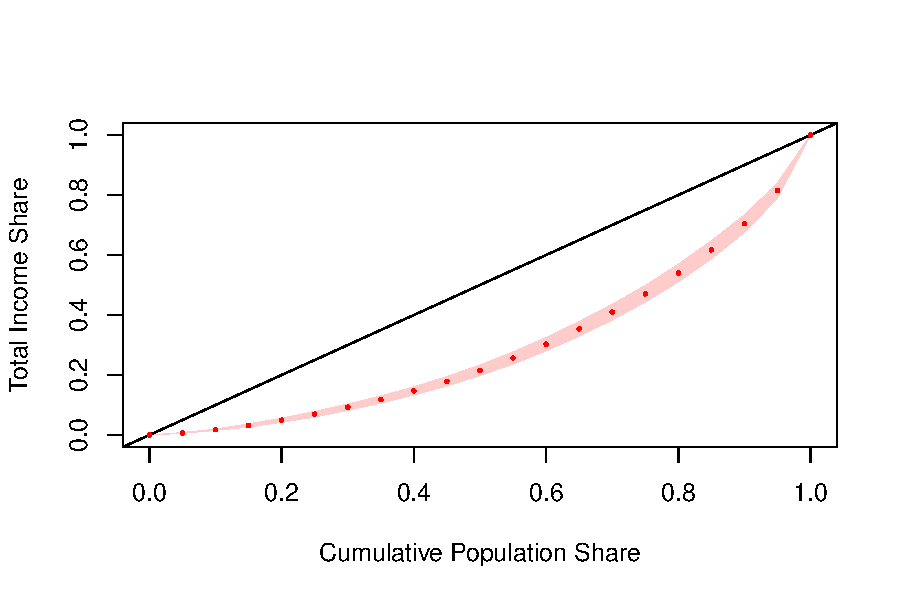
\includegraphics[width=0.65\linewidth,height=\textheight,keepaspectratio]{chapters/../figures/fig-lorenz-1.pdf}

}

\caption{\label{fig-lorenz}Curva de Lorenz estimada para el ingreso per
cápita}

\end{figure}%

El argumento \texttt{formula\ =\ \textasciitilde{}Income} especifica la
variable de ingreso sobre la cual se calculará la distribución
acumulada. El argumento \texttt{design\ =\ gini\_design} indica el
objeto de diseño muestral previamente definido, el cual contiene la
información relacionada con pesos, estratos y conglomerados de la
encuesta. Por su parte, \texttt{quantiles\ =\ seq(0,\ 1,\ .05)} define
los puntos de la distribución en los cuales se evaluará la curva de
Lorenz, generando proporciones acumuladas desde 0 hasta 1 en incrementos
de 0.05. Finalmente, el argumento \texttt{alpha\ =\ .05} establece un
nivel de significación del 5\%, lo que equivale a construir intervalos
de confianza del 95\% para las estimaciones asociadas a la curva.

A partir de la figura~\ref{fig-lorenz}, se observa un grado considerable
de desigualdad en la distribución del ingreso per cápita, dado que la
curva de Lorenz se sitúa claramente por debajo de la línea de igualdad
perfecta. Su marcada curvatura muestra que los grupos ubicados en la
parte inferior de la distribución concentran una proporción reducida del
ingreso total, mientras que una participación considerable se acumula
entre las personas de mayores ingresos. La curva se separa de la línea
de igualdad en los tramos intermedios y vuelve a encontrarse con ella al
acumular el total de la población y del ingreso. La reducida
participación acumulada del ingreso en los primeros tramos muestra su
concentración entre las personas de mayores ingresos. Por su parte, la
banda sombreada representa la incertidumbre asociada a la estimación de
la curva.

\subsection{Correlaciones}\label{estimacion-de-la-correlacion}

En el capítulo anterior se estudió asociación entre categorías. Ahora se
describe la relación lineal entre magnitudes numéricas. En el estudio de
encuestas de hogares, además de describir variables de forma individual,
es importante analizar cómo se relacionan dos variables entre sí. Una de
las herramientas más utilizadas para este propósito es el coeficiente de
correlación de Pearson, el cual mide la fuerza y la dirección de la
relación lineal entre dos variables numéricas. Este coeficiente toma
valores entre --1 y 1. Un valor positivo indica que ambas variables
tienden a aumentar simultáneamente, mientras que un valor negativo
señala que cuando una variable aumenta, la otra tiende a disminuir. Por
su parte, valores cercanos a cero sugieren la ausencia de una relación
lineal fuerte entre las variables analizadas. Por ejemplo, en una
encuesta de hogares puede ser de interés estudiar qué tan fuerte es la
asociación entre el ingreso per cápita y su nivel de gasto. Este tipo de
análisis permite comprender mejor los patrones económicos y sociales en
la población.

Supóngase que se dispone de dos variables numéricas de interés,
denotadas por \(x\) y \(y\), observadas en la encuesta compleja. De
acuerdo con Heeringa et~al.
(\citeproc{ref-HeeringaWestBerglund2017}{2017}), la asociación lineal
entre ambas variables puede estimarse mediante el coeficiente de
correlación de Pearson ponderado, definido como la covarianza ponderada
entre \(x\) y \(y\) dividida por el producto de sus desviaciones
estándar ponderadas. Esta estandarización elimina la influencia de las
unidades de medida y permite evaluar tanto la dirección como la
intensidad de la relación lineal. Si \(\hat{\bar{x}}\) y
\(\hat{\bar{y}}\) representan las estimaciones de las medias
poblacionales de \(x\) y \(y\), respectivamente, el coeficiente de
correlación ponderado se expresa como:

\begin{equation}\protect\phantomsection\label{eq-correlacion-ponderada}{
\hat{\rho}_{xy} = \frac{\displaystyle \sum_{h} \sum_{i} \sum_{k} w_{hik} (y_{hik} - \hat{\bar{y}})(x_{hik} - \hat{\bar{x}})} {\sqrt{\displaystyle \sum_{h} \sum_{i} \sum_{k} w_{hik} (y_{hik} - \hat{\bar{y}})^2} \sqrt{\displaystyle \sum_{h} \sum_{i} \sum_{k} w_{hik} (x_{hik} - \hat{\bar{x}})^2}}
}\end{equation}

La covarianza entre variables describe su distribución conjunta en la
población. Es distinta de la covarianza entre estimadores obtenida con
\texttt{vcov()} en los contrastes del capítulo anterior.

El siguiente código computacional utiliza \texttt{svyvar()} del paquete
\texttt{survey} para estimar la matriz de varianzas y covarianzas del
ingreso y el gasto per cápita, incorporando el diseño muestral. Luego
organiza los resultados con los nombres de las variables para
presentarlos en la tabla~\ref{tbl-covarianza}. Esta matriz también
permite calcular la correlación entre ambas variables.

\begin{Shaded}
\begin{Highlighting}[]
\NormalTok{cov\_matrix }\OtherTok{\textless{}{-}} \FunctionTok{svyvar}\NormalTok{(}\SpecialCharTok{\textasciitilde{}}\NormalTok{Income }\SpecialCharTok{+}\NormalTok{ Expenditure, }\AttributeTok{design =}\NormalTok{ survey\_design)}
\end{Highlighting}
\end{Shaded}

\begin{Shaded}
\begin{Highlighting}[]
\NormalTok{income\_expenditure\_covariance\_table }\OtherTok{\textless{}{-}} \FunctionTok{data.frame}\NormalTok{(}
  \AttributeTok{Variable =} \FunctionTok{rownames}\NormalTok{(cov\_matrix),}
  \FunctionTok{as.matrix}\NormalTok{(cov\_matrix)}
\NormalTok{) }\SpecialCharTok{\%\textgreater{}\%}
  \FunctionTok{slice}\NormalTok{(}\DecValTok{1}\SpecialCharTok{:}\DecValTok{2}\NormalTok{)}

\NormalTok{income\_expenditure\_covariance\_table}
\end{Highlighting}
\end{Shaded}

{

\begin{longtable}[]{@{}llrr@{}}

\caption{\label{tbl-covarianza}Matriz de varianzas y covarianzas
ponderada entre ingreso y gasto}

\tabularnewline

\toprule\noalign{}
& Variable & Ingreso & Gasto \\
\midrule\noalign{}
\endhead
\bottomrule\noalign{}
\endlastfoot
Income & Income & 243719 & 98337 \\
Expenditure & Expenditure & 98337 & 77887 \\

\end{longtable}

}

La función \texttt{svyvar} estima la matriz de varianzas y covarianzas
considerando el diseño muestral. A partir de dicha matriz puede
obtenerse la correlación aplicando las siguientes instrucciones:

\begin{Shaded}
\begin{Highlighting}[]
\NormalTok{cov\_xy }\OtherTok{\textless{}{-}}\NormalTok{ cov\_matrix[}\DecValTok{1}\NormalTok{, }\DecValTok{2}\NormalTok{]}
\NormalTok{sd\_x }\OtherTok{\textless{}{-}} \FunctionTok{sqrt}\NormalTok{(cov\_matrix[}\DecValTok{1}\NormalTok{, }\DecValTok{1}\NormalTok{])}
\NormalTok{sd\_y }\OtherTok{\textless{}{-}} \FunctionTok{sqrt}\NormalTok{(cov\_matrix[}\DecValTok{2}\NormalTok{, }\DecValTok{2}\NormalTok{])}

\NormalTok{weighted\_cor }\OtherTok{\textless{}{-}}\NormalTok{ cov\_xy }\SpecialCharTok{/}\NormalTok{ (sd\_x }\SpecialCharTok{*}\NormalTok{ sd\_y)}
\NormalTok{weighted\_cor}
\end{Highlighting}
\end{Shaded}

\begin{verbatim}
[1] 0.714
\end{verbatim}

Si además se desea realizar inferencia estadística sobre la correlación,
por ejemplo obtener errores estándar o intervalos de confianza, pueden
utilizarse métodos de replicación compatibles con el paquete
\texttt{survey}. El siguiente código computacional ilustra otra opción:
estimar directamente la correlación entre ingreso y gasto con
\texttt{svycor()} del paquete \texttt{jtools}
(\citeproc{ref-jtools2026}{Long 2026}).

\begin{Shaded}
\begin{Highlighting}[]
\FunctionTok{library}\NormalTok{(jtools)}

\FunctionTok{svycor}\NormalTok{(}
  \SpecialCharTok{\textasciitilde{}}\NormalTok{Income }\SpecialCharTok{+}\NormalTok{ Expenditure,}
  \AttributeTok{design =}\NormalTok{ survey\_design,}
  \AttributeTok{sig.stats =} \ConstantTok{FALSE}
\NormalTok{)}
\end{Highlighting}
\end{Shaded}

\begin{verbatim}
            Income Expenditure
Income        1.00        0.71
Expenditure   0.71        1.00
\end{verbatim}

La llamada anterior presenta la correlación sin solicitar pruebas ni
intervalos. La correlación entre el ingreso y el gasto es relativamente
alta, con un coeficiente de Pearson estimado de 0,71. Esto indica que,
en términos generales, los hogares con mayores ingresos tienden a
registrar también niveles de gasto más elevados. Los valores iguales a 1
en la diagonal corresponden a la correlación de cada variable consigo
misma. Finalmente, este resultado refleja una asociación lineal y no
debe interpretarse como evidencia de una relación causal.

\section{Pruebas de hipótesis}\label{pruebas-de-hipotesis}

En el análisis de datos provenientes de encuestas de hogares no basta
con estudiar cada variable de manera aislada, sino que también es
fundamental comparar grupos y evaluar si las diferencias observadas
entre ellos reflejan desigualdades reales en la población o si podrían
explicarse simplemente por el error de muestreo. Por ejemplo, una
pregunta de interés consiste en determinar si existen diferencias
estadísticamente significativas en el ingreso medio entre hogares
dirigidos por hombres y hogares dirigidos por mujeres. Este tipo de
análisis permite identificar brechas sociales y económicas, además de
generar evidencia útil para el diseño y evaluación de políticas
públicas.

La lógica de hipótesis nula y alternativa se introdujo en la
Sección~\ref{sec-pruebas-de-hipotesis-sobre-proporciones}. Aquí se
conserva ese mismo marco referencial. Por ejemplo, para la diferencia de
medias se estima la diferencia puntual, junto con su error estándar,
incorporando la covarianza entre estimaciones de dominios. De esta
manera, supóngase que \(\bar{y}_1\) y \(\bar{y}_2\) representan las
medias poblacionales de una variable \(y\) en dos dominios distintos,
como los hogares con jefatura masculina y femenina. En este caso, el
parámetro de interés corresponde a la diferencia entre ambas medias:

\[
\Delta = \bar{y}_1 - \bar{y}_2
\]

Su estimador muestral se define como:

\[
\hat{\Delta} = \hat{\bar{y}}_1 - \hat{\bar{y}}_2
\]

Su error estándar se estima mediante la siguiente expresión:

\[
\widehat{se}(\hat{\Delta}) =
\sqrt{
\widehat{Var}(\hat{\bar{y}}_1)
+
\widehat{Var}(\hat{\bar{y}}_2)
-
2\widehat{Cov}(\hat{\bar{y}}_1, \hat{\bar{y}}_2)
}
\]

La presencia del término de covarianza, ya estudiado al comparar
proporciones, es importante porque las estimaciones de ambos dominios
suelen provenir de la misma muestra y, por tanto, no necesariamente son
independientes. Una vez calculado el estimador y su error estándar, se
aplica el procedimiento descrito en la
Sección~\ref{sec-pruebas-de-hipotesis-sobre-proporciones}, sustituyendo
\(\hat{\Delta}_p\) por \(\hat{\Delta}\). El estadístico de prueba, su
distribución de referencia y el intervalo de confianza se construyen de
la misma manera, utilizando los grados de libertad devueltos por
\texttt{svyttest()}.

El siguiente código computacional crea primero el objeto
\texttt{survey\_design\_heads}, que conserva únicamente las
observaciones correspondientes a las personas jefas de hogar,
identificadas mediante \texttt{PersonID\ ==\ "idPer01"}, sin perder las
características del diseño muestral. Posteriormente, la función
\texttt{svyttest()} compara el ingreso medio entre las categorías de la
variable \texttt{Sex}. Se fija \texttt{Female} como referencia: el
resultado representa hombres menos mujeres. La prueba devuelve un
intervalo del 95 \%. Para este ejemplo se aplica la convención del
capítulo 3: se conserva el registro de la persona principal de cada
hogar y se utiliza su factor de expansión como aproximación al peso del
hogar. Así se compara el ingreso per cápita entre hogares con jefatura
masculina y femenina, con las limitaciones señaladas para esta
aproximación. Finalmente, se reúnen la diferencia estimada, el
estadístico, el valor-\emph{p}, los grados de libertad y el intervalo de
confianza.

\begin{Shaded}
\begin{Highlighting}[]
\NormalTok{survey\_design\_heads }\OtherTok{\textless{}{-}}\NormalTok{ survey\_design }\SpecialCharTok{\%\textgreater{}\%}
  \FunctionTok{filter}\NormalTok{(PersonID }\SpecialCharTok{==} \StringTok{"idPer01"}\NormalTok{) }\SpecialCharTok{\%\textgreater{}\%}
  \FunctionTok{mutate}\NormalTok{(}\AttributeTok{Sex =} \FunctionTok{factor}\NormalTok{(Sex, }\AttributeTok{levels =} \FunctionTok{c}\NormalTok{(}\StringTok{"Female"}\NormalTok{, }\StringTok{"Male"}\NormalTok{)))}

\NormalTok{ttest\_sex }\OtherTok{\textless{}{-}} \FunctionTok{svyttest}\NormalTok{(Income }\SpecialCharTok{\textasciitilde{}}\NormalTok{ Sex, }\AttributeTok{design =}\NormalTok{ survey\_design\_heads)}
\end{Highlighting}
\end{Shaded}

\begin{Shaded}
\begin{Highlighting}[]
\NormalTok{df\_res }\OtherTok{\textless{}{-}} \FunctionTok{tibble}\NormalTok{(}
  \AttributeTok{estimated\_difference =}\NormalTok{ ttest\_sex}\SpecialCharTok{$}\NormalTok{estimate,}
  \AttributeTok{statistic =}\NormalTok{ ttest\_sex}\SpecialCharTok{$}\NormalTok{statistic,}
  \AttributeTok{p\_value =}\NormalTok{ ttest\_sex}\SpecialCharTok{$}\NormalTok{p.value,}
  \AttributeTok{gl =}\NormalTok{ ttest\_sex}\SpecialCharTok{$}\NormalTok{parameter,}
  \AttributeTok{ci\_lower =}\NormalTok{ ttest\_sex}\SpecialCharTok{$}\NormalTok{conf.int[}\DecValTok{1}\NormalTok{],}
  \AttributeTok{ci\_upper =}\NormalTok{ ttest\_sex}\SpecialCharTok{$}\NormalTok{conf.int[}\DecValTok{2}\NormalTok{]}
\NormalTok{)}
\NormalTok{income\_sex\_test\_table }\OtherTok{\textless{}{-}}\NormalTok{ df\_res}

\NormalTok{income\_sex\_test\_table}
\end{Highlighting}
\end{Shaded}

{

\begin{longtable}[]{@{}rrrrrr@{}}

\caption{\label{tbl-ttest-sexo}Diferencia de ingreso per cápita entre
personas jefas de hogar por sexo}

\tabularnewline

\toprule\noalign{}
Diferencia & Estadístico t & Valor p & gl & LI 95 \% & LS 95 \% \\
\midrule\noalign{}
\endhead
\bottomrule\noalign{}
\endlastfoot
122 & 2.76 & 0.007 & 118 & 34.7 & 210 \\

\end{longtable}

}

A partir de los resultados presentados en la tabla~\ref{tbl-ttest-sexo},
se estima que el ingreso per cápita de los hogares asociado a los
hombres jefes de hogar es aproximadamente 122 dólares mayor al asociado
a las mujeres jefas de hogar. Dado que el valor \(p\) obtenido es
0.00664, inferior al nivel de significación establecido de
\(\alpha = 0,05\), se rechaza la hipótesis nula de igualdad de medias y
se concluye que la diferencia observada es estadísticamente
significativa. Esta conclusión es consistente con el intervalo de
confianza del 95 \%, que no incluye el valor cero. En conjunto, los
resultados aportan evidencia de que, en la población representada por la
encuesta, el ingreso per cápita asociado a las mujeres jefas de hogar es
significativamente menor que el asociado a los hombres jefes de hogar,
bajo el diseño y el dominio considerados.

\section{Estimación de contrastes}\label{estimacion-de-contrastes}

La comparación de medias presentada en la sección anterior puede
extenderse a otras diferencias de interés entre grupos poblacionales.
Por ejemplo, se pueden comparar los ingresos medios entre regiones o las
razones de gasto e ingreso entre hogares con jefatura masculina y
femenina. Estas diferencias se expresan mediante contrastes que combinan
las estimaciones de cada grupo y utilizan sus varianzas y covarianzas
para cuantificar la incertidumbre. En esta sección se muestra cómo
construirlos y cómo estimar varias comparaciones por pares, cada una con
su respectivo intervalo de confianza.

La definición general de contraste, sus coeficientes y las funciones
\texttt{svyby()}, \texttt{vcov()} y \texttt{svycontrast()} se
presentaron en la
Sección~\ref{sec-contrastes-y-diferencias-de-proporciones}. Aquí se
sustituyen las proporciones por medias y, después, por razones, aunque
se conserva la matriz de covarianzas mediante \texttt{covmat\ =\ TRUE}.
Por ejemplo, si se quiere comparar los ingresos medios de dos
subpoblaciones particulares (las regiones Norte y Sur) se puede usar el
contraste \(\bar{y}_{Norte} - \bar{y}_{Sur}\). Dado que la muestra cubre
cinco regiones en total, el contraste debe construirse asignando
coeficientes únicamente a las regiones involucradas en la comparación y
dejando coeficientes iguales a cero para las demás regiones. De esta
manera, el contraste se define como:

\[
1\times\hat{\bar{y}}_{Norte}+\left(-1\right)\times\hat{\bar{y}}_{Sur}+0\times\hat{\bar{y}}_{Centro}+0\times\hat{\bar{y}}_{Occidente}+0\times\hat{\bar{y}}_{Oriente}.
\]

Esta expresión indica que el contraste corresponde a la diferencia entre
las medias estimadas de las regiones Norte y Sur, mientras que las demás
regiones no participan en la comparación. De forma matricial, el
contraste puede escribirse como:

\[
 \left[1,\,-1,\,0,\,0,\,0\right]
 \times
 \left[\begin{array}{c}
\hat{\bar{y}}_{Norte}\\
\hat{\bar{y}}_{Sur}\\
\hat{\bar{y}}_{Centro}\\
\hat{\bar{y}}_{Occidente}\\
\hat{\bar{y}}_{Oriente}
\end{array}\right].
\]

En consecuencia, el vector de contraste asociado a esta comparación es
\(\left[1,\,-1,\,0,\,0,\,0\right]\), donde los coeficientes positivos y
negativos indican las poblaciones que se desean comparar y los ceros
representan las poblaciones excluidas del contraste. En \texttt{R},
estos procedimientos se encuentran disponibles mediante la función
\texttt{svycontrast()} del paquete \texttt{survey}. El siguiente código
computacional estima las medias regionales de ingreso, conserva sus
covarianzas y organiza los resultados para presentarlos en la
tabla~\ref{tbl-prom-region}.

\begin{Shaded}
\begin{Highlighting}[]
\NormalTok{region\_mean\_contrast }\OtherTok{\textless{}{-}} \FunctionTok{svyby}\NormalTok{(}
  \AttributeTok{formula =} \SpecialCharTok{\textasciitilde{}}\NormalTok{ Income,}
  \AttributeTok{by =} \SpecialCharTok{\textasciitilde{}}\NormalTok{ Region,}
  \AttributeTok{design =}\NormalTok{ survey\_design,}
  \AttributeTok{FUN =}\NormalTok{ svymean,}
  \AttributeTok{na.rm =} \ConstantTok{TRUE}\NormalTok{,}
  \AttributeTok{covmat =} \ConstantTok{TRUE}\NormalTok{,}
  \AttributeTok{vartype =} \FunctionTok{c}\NormalTok{(}\StringTok{"se"}\NormalTok{, }\StringTok{"ci"}\NormalTok{)}
\NormalTok{)}
\end{Highlighting}
\end{Shaded}

\begin{Shaded}
\begin{Highlighting}[]
\NormalTok{regional\_income\_means\_table }\OtherTok{\textless{}{-}}\NormalTok{ region\_mean\_contrast}

\NormalTok{regional\_income\_means\_table}
\end{Highlighting}
\end{Shaded}

{

\begin{longtable}[]{@{}lrrrr@{}}

\caption{\label{tbl-prom-region}Ingreso medio estimado por región}

\tabularnewline

\toprule\noalign{}
Región & Ingreso & EE & LI 95 \% & LS 95 \% \\
\midrule\noalign{}
\endhead
\bottomrule\noalign{}
\endlastfoot
North & 552 & 55.4 & 444 & 661 \\
South & 626 & 62.4 & 503 & 748 \\
Central & 651 & 61.5 & 530 & 771 \\
West & 517 & 46.2 & 426 & 608 \\
East & 542 & 71.7 & 401 & 682 \\

\end{longtable}

}

La función \texttt{svyby()} estima el ingreso medio por región, de
acuerdo con el diseño de muestreo \texttt{survey\_design}. El argumento
\texttt{formula\ =\ \textasciitilde{}Income} especifica la variable
numérica de interés, mientras que
\texttt{by\ =\ \textasciitilde{}Region} define los dominios para los
cuales se realizará la estimación. La opción \texttt{FUN\ =\ svymean}
indica que debe calcularse la media del ingreso en cada región y
\texttt{na.rm\ =\ TRUE} excluye las observaciones con valores faltantes.
Por su parte, \texttt{vartype\ =\ c("se",\ "ci")} solicita el error
estándar y el intervalo de confianza de cada media estimada. Estos
intervalos utilizan la aproximación normal, como se explica en la
Sección~\ref{sec-contrastes-y-diferencias-de-proporciones}. Finalmente,
\texttt{covmat\ =\ TRUE} calcula la matriz de varianzas y covarianzas
entre las estimaciones regionales, lo que permite realizar
posteriormente contrastes o comparaciones entre ellas.

Luego, la función \texttt{svycontrast()} devuelve el contraste estimado
y su error estándar, como se muestra en la tabla~\ref{tbl-contraste-ns}.
Los argumentos de esta función son los promedios de los ingresos
estimados (\texttt{stat}) y las constantes de contraste
(\texttt{contrasts}). Para los contrastes lineales de esta sección, el
error estándar se calcula a partir de la matriz de varianzas y
covarianzas de las estimaciones que se comparan. Si se aplica
\texttt{confint()} directamente al resultado de \texttt{svycontrast()},
el intervalo de Wald utiliza por defecto un cuantil normal. En las
tablas de contrastes de esta sección se adopta una distribución \(t\) de
Student con los grados de libertad del diseño utilizado en cada
comparación. Los límites se calculan explícitamente con \texttt{qt()} y
\texttt{degf()}. Para estos contrastes se obtienen los mismos límites al
usar \texttt{confint()} con \texttt{df\ =\ degf(diseño)} y el mismo
nivel de confianza. El siguiente código computacional estima la
diferencia entre los ingresos medios de Norte y Sur mediante
\texttt{svycontrast()} y reúne el contraste, su error estándar y su
intervalo de confianza para presentarlos en la tabla.

\begin{Shaded}
\begin{Highlighting}[]
\NormalTok{contrast\_region\_ns }\OtherTok{\textless{}{-}} \FunctionTok{svycontrast}\NormalTok{(}
  \AttributeTok{stat =}\NormalTok{ region\_mean\_contrast,}
  \AttributeTok{contrasts =} \FunctionTok{list}\NormalTok{(}
    \AttributeTok{north\_south\_difference =} \FunctionTok{c}\NormalTok{(}\AttributeTok{North =} \DecValTok{1}\NormalTok{, }\AttributeTok{South =} \SpecialCharTok{{-}}\DecValTok{1}\NormalTok{)}
\NormalTok{  )}
\NormalTok{)}
\end{Highlighting}
\end{Shaded}

\begin{Shaded}
\begin{Highlighting}[]
\NormalTok{critical }\OtherTok{\textless{}{-}} \FunctionTok{qt}\NormalTok{(}\FloatTok{0.975}\NormalTok{, }\AttributeTok{df =} \FunctionTok{degf}\NormalTok{(survey\_design))}
\NormalTok{north\_south\_income\_contrast\_table }\OtherTok{\textless{}{-}} \FunctionTok{tibble}\NormalTok{(}
  \AttributeTok{contrast =} \FunctionTok{names}\NormalTok{(}\FunctionTok{coef}\NormalTok{(contrast\_region\_ns)),}
  \AttributeTok{estimate =} \FunctionTok{as.numeric}\NormalTok{(}\FunctionTok{coef}\NormalTok{(contrast\_region\_ns)),}
  \AttributeTok{standard\_error =} \FunctionTok{as.numeric}\NormalTok{(}\FunctionTok{SE}\NormalTok{(contrast\_region\_ns)),}
  \AttributeTok{lower =}\NormalTok{ estimate }\SpecialCharTok{{-}}\NormalTok{ critical }\SpecialCharTok{*}\NormalTok{ standard\_error,}
  \AttributeTok{upper =}\NormalTok{ estimate }\SpecialCharTok{+}\NormalTok{ critical }\SpecialCharTok{*}\NormalTok{ standard\_error}
\NormalTok{)}

\NormalTok{north\_south\_income\_contrast\_table}
\end{Highlighting}
\end{Shaded}

{

\begin{longtable}[]{@{}lrrrr@{}}

\caption{\label{tbl-contraste-ns}Contraste de ingresos medios: región
North menos región South}

\tabularnewline

\toprule\noalign{}
Contraste & Estimación & EE & LI 95 \% & LS 95 \% \\
\midrule\noalign{}
\endhead
\bottomrule\noalign{}
\endlastfoot
north\_south\_difference & -73.4 & 83.4 & -239 & 91.8 \\

\end{longtable}

}

La estimación de la diferencia de medias indica que el ingreso promedio
en la región Norte es aproximadamente 73,4 dólares inferior al observado
en la región Sur. Sin embargo, el error estándar de 83,4 es mayor que la
diferencia estimada, lo que refleja una incertidumbre considerable. Por
tanto, no hay evidencia suficiente para concluir que exista una
diferencia estadísticamente significativa entre ambas regiones. Nótese
que estos mismos resultados podrían obtenerse realizando explícitamente
el proceso de construcción del estimador del contraste y de su varianza
estimada. El siguiente código computacional inicia este cálculo directo
restando el ingreso medio estimado de Sur al de Norte.

\begin{Shaded}
\begin{Highlighting}[]
\CommentTok{\# Paso 1: diferencia de las estimaciones (North {-} South)}
\NormalTok{region\_income\_mean }\OtherTok{\textless{}{-}} \FunctionTok{setNames}\NormalTok{(}
  \FunctionTok{as.numeric}\NormalTok{(region\_mean\_contrast[[}\StringTok{"Income"}\NormalTok{]]),}
\NormalTok{  region\_mean\_contrast[[}\StringTok{"Region"}\NormalTok{]]}
\NormalTok{)}

\NormalTok{region\_income\_mean[}\StringTok{"North"}\NormalTok{] }\SpecialCharTok{{-}}\NormalTok{ region\_income\_mean[}\StringTok{"South"}\NormalTok{]}
\end{Highlighting}
\end{Shaded}

\begin{verbatim}
North 
-73.4 
\end{verbatim}

El siguiente código computacional obtiene la matriz de varianzas y
covarianzas y la organiza con los nombres de las regiones para
presentarla en la tabla~\ref{tbl-vcov-region}. De ella se extraen los
elementos correspondientes a Norte y Sur. Las covarianzas estimadas
entre las regiones son todas nulas, lo que resulta coherente con el
diseño muestral, dado que la estratificación se realizó por región y la
selección de la muestra se efectuó de manera independiente en cada
estrato. En consecuencia, los estimadores regionales no comparten
unidades muestrales y su covarianza bajo el diseño es igual a cero.

\begin{Shaded}
\begin{Highlighting}[]
\CommentTok{\# Paso 2: matriz de varianzas y covarianzas}
\NormalTok{region\_vcov }\OtherTok{\textless{}{-}} \FunctionTok{vcov}\NormalTok{(region\_mean\_contrast)}
\end{Highlighting}
\end{Shaded}

\begin{Shaded}
\begin{Highlighting}[]
\NormalTok{df\_vcov }\OtherTok{\textless{}{-}}\NormalTok{ region\_vcov }\SpecialCharTok{\%\textgreater{}\%}
  \FunctionTok{as.data.frame}\NormalTok{() }\SpecialCharTok{\%\textgreater{}\%}
\NormalTok{  tibble}\SpecialCharTok{::}\FunctionTok{rownames\_to\_column}\NormalTok{(}\StringTok{"Region"}\NormalTok{)}

\NormalTok{regional\_income\_covariance\_table }\OtherTok{\textless{}{-}}\NormalTok{ df\_vcov}

\NormalTok{regional\_income\_covariance\_table}
\end{Highlighting}
\end{Shaded}

{

\begin{longtable}[]{@{}lrrrrr@{}}

\caption{\label{tbl-vcov-region}Matriz de varianzas y covarianzas de los
ingresos medios por región}

\tabularnewline

\toprule\noalign{}
Región & Norte & Sur & Centro & Occidente & Oriente \\
\midrule\noalign{}
\endhead
\bottomrule\noalign{}
\endlastfoot
North & 3065 & 0 & 0 & 0 & 0 \\
South & 0 & 3894 & 0 & 0 & 0 \\
Central & 0 & 0 & 3778 & 0 & 0 \\
West & 0 & 0 & 0 & 2136 & 0 \\
East & 0 & 0 & 0 & 0 & 5136 \\

\end{longtable}

}

Para calcular el error estándar de la diferencia (contraste) se usarán
las propiedades de la varianza, de la siguiente forma:

\[
\widehat{se}\left(\hat{\bar{y}}_{Norte}-\hat{\bar{y}}_{Sur}\right)=\sqrt{\widehat {Var}\left(\hat{\bar{y}}_{Norte}\right)+
\widehat{Var}\left(\hat{\bar{y}}_{Sur}\right)-
2\, \widehat{Cov}\left(\hat{\bar{y}}_{Norte},\hat{\bar{y}}_{Sur}\right)}
\]

Para evitar inconsistencias por redondeo, el siguiente código
computacional calcula el error estándar de la diferencia Norte menos Sur
directamente a partir de la matriz estimada de varianzas y covarianzas.

\begin{Shaded}
\begin{Highlighting}[]
\FunctionTok{sqrt}\NormalTok{(}
\NormalTok{  region\_vcov[}\StringTok{"North"}\NormalTok{, }\StringTok{"North"}\NormalTok{] }\SpecialCharTok{+}
\NormalTok{    region\_vcov[}\StringTok{"South"}\NormalTok{, }\StringTok{"South"}\NormalTok{] }\SpecialCharTok{{-}}
    \DecValTok{2} \SpecialCharTok{*}\NormalTok{ region\_vcov[}\StringTok{"North"}\NormalTok{, }\StringTok{"South"}\NormalTok{]}
\NormalTok{)}
\end{Highlighting}
\end{Shaded}

\begin{verbatim}
[1] 83.4
\end{verbatim}

Este resultado corresponde al mismo obtenido anteriormente con la
función \texttt{svycontrast()}.

Además de comparar únicamente dos poblaciones, los contrastes permiten
estimar varias comparaciones de interés entre diferentes grupos. Por
ejemplo, supóngase que se desea comparar los ingresos medios entre
distintas regiones geográficas. En particular, podrían considerarse
contrastes como \(\bar{y}_{Norte} - \bar{y}_{Centro}\),
\(\bar{y}_{Sur} - \bar{y}_{Centro}\) y
\(\bar{y}_{Occidente} - \bar{y}_{Oriente}\). Cada una de estas
expresiones representa un contraste lineal específico entre medias
regionales. De manera conjunta, dichos contrastes pueden organizarse
mediante la siguiente matriz de contrastes:

\[
\left[\begin{array}{ccccc}
1 & 0 & -1 & 0 & 0\\
0 & 1 & -1 & 0 & 0\\
0 & 0 & 0 & 1 & -1
\end{array}\right]
\]

Se estiman varias diferencias, sin realizar aquí una prueba conjunta ni
un ajuste de comparaciones múltiples. El orden de columnas es Norte,
Sur, Centro, Occidente y Oriente; el código asigna coeficientes por
nombre. En esta matriz, cada fila define un contraste distinto y cada
columna corresponde a una de las regiones consideradas en el análisis.
Los coeficientes positivos y negativos indican las medias que participan
en cada comparación, mientras que los ceros representan las regiones que
no intervienen en el contraste correspondiente. El siguiente código
computacional estima estos contrastes y organiza las diferencias
regionales, sus errores estándar y sus intervalos de confianza para
presentarlos en la tabla~\ref{tbl-contraste-regiones}.

\begin{Shaded}
\begin{Highlighting}[]
\NormalTok{contrast\_regions }\OtherTok{\textless{}{-}} \FunctionTok{svycontrast}\NormalTok{(}
  \AttributeTok{stat =}\NormalTok{ region\_mean\_contrast,}
  \AttributeTok{contrasts =} \FunctionTok{list}\NormalTok{(}
    \AttributeTok{north\_center =} \FunctionTok{c}\NormalTok{(}\AttributeTok{North =} \DecValTok{1}\NormalTok{, }\AttributeTok{Central =} \SpecialCharTok{{-}}\DecValTok{1}\NormalTok{),}
    \AttributeTok{south\_center =} \FunctionTok{c}\NormalTok{(}\AttributeTok{South =} \DecValTok{1}\NormalTok{, }\AttributeTok{Central =} \SpecialCharTok{{-}}\DecValTok{1}\NormalTok{),}
    \AttributeTok{west\_east =} \FunctionTok{c}\NormalTok{(}\AttributeTok{West =} \DecValTok{1}\NormalTok{, }\AttributeTok{East =} \SpecialCharTok{{-}}\DecValTok{1}\NormalTok{)}
\NormalTok{  )}
\NormalTok{)}
\end{Highlighting}
\end{Shaded}

\begin{Shaded}
\begin{Highlighting}[]
\NormalTok{critical }\OtherTok{\textless{}{-}} \FunctionTok{qt}\NormalTok{(}\FloatTok{0.975}\NormalTok{, }\AttributeTok{df =} \FunctionTok{degf}\NormalTok{(survey\_design))}
\NormalTok{regional\_income\_contrasts\_table }\OtherTok{\textless{}{-}} \FunctionTok{tibble}\NormalTok{(}
  \AttributeTok{contrast =} \FunctionTok{names}\NormalTok{(}\FunctionTok{coef}\NormalTok{(contrast\_regions)),}
  \AttributeTok{estimate =} \FunctionTok{as.numeric}\NormalTok{(}\FunctionTok{coef}\NormalTok{(contrast\_regions)),}
  \AttributeTok{standard\_error =} \FunctionTok{as.numeric}\NormalTok{(}\FunctionTok{SE}\NormalTok{(contrast\_regions)),}
  \AttributeTok{lower =}\NormalTok{ estimate }\SpecialCharTok{{-}}\NormalTok{ critical }\SpecialCharTok{*}\NormalTok{ standard\_error,}
  \AttributeTok{upper =}\NormalTok{ estimate }\SpecialCharTok{+}\NormalTok{ critical }\SpecialCharTok{*}\NormalTok{ standard\_error}
\NormalTok{)}

\NormalTok{regional\_income\_contrasts\_table}
\end{Highlighting}
\end{Shaded}

{

\begin{longtable}[]{@{}lrrrr@{}}

\caption{\label{tbl-contraste-regiones}Contrastes de ingresos medios
entre regiones}

\tabularnewline

\toprule\noalign{}
Contraste & Estimación & EE & LI 95 \% & LS 95 \% \\
\midrule\noalign{}
\endhead
\bottomrule\noalign{}
\endlastfoot
north\_center & -98.4 & 82.7 & -262 & 65.4 \\
south\_center & -25.0 & 87.6 & -198 & 148.4 \\
west\_east & -24.7 & 85.3 & -194 & 144.1 \\

\end{longtable}

}

También pueden construirse contrastes para comparar el ingreso per
cápita según el sexo de la persona jefa del hogar. El siguiente código
computacional utiliza \texttt{survey\_design\_heads} para estimar la
media de cada grupo y organizar las estimaciones y sus medidas de
precisión, presentadas en la tabla~\ref{tbl-prom-sexo}.

\begin{Shaded}
\begin{Highlighting}[]
\NormalTok{sex\_mean\_contrast }\OtherTok{\textless{}{-}} \FunctionTok{svyby}\NormalTok{(}
  \AttributeTok{formula =} \SpecialCharTok{\textasciitilde{}}\NormalTok{ Income,}
  \AttributeTok{by =} \SpecialCharTok{\textasciitilde{}}\NormalTok{ Sex,}
  \AttributeTok{design =}\NormalTok{ survey\_design\_heads,}
  \AttributeTok{FUN =}\NormalTok{ svymean,}
  \AttributeTok{na.rm =} \ConstantTok{TRUE}\NormalTok{,}
  \AttributeTok{covmat =} \ConstantTok{TRUE}\NormalTok{,}
  \AttributeTok{vartype =} \FunctionTok{c}\NormalTok{(}\StringTok{"se"}\NormalTok{, }\StringTok{"ci"}\NormalTok{)}
\NormalTok{)}
\end{Highlighting}
\end{Shaded}

\begin{Shaded}
\begin{Highlighting}[]
\NormalTok{income\_means\_by\_sex\_table }\OtherTok{\textless{}{-}}\NormalTok{ sex\_mean\_contrast }\SpecialCharTok{\%\textgreater{}\%}
  \FunctionTok{as\_tibble}\NormalTok{()}

\NormalTok{income\_means\_by\_sex\_table}
\end{Highlighting}
\end{Shaded}

{

\begin{longtable}[]{@{}lrrrr@{}}

\caption{\label{tbl-prom-sexo}Ingreso per cápita asociado a personas
jefas de hogar, por sexo}

\tabularnewline

\toprule\noalign{}
Sexo & Ingreso & EE & LI 95 \% & LS 95 \% \\
\midrule\noalign{}
\endhead
\bottomrule\noalign{}
\endlastfoot
Female & 442 & 23.5 & 396 & 488 \\
Male & 564 & 34.0 & 498 & 631 \\

\end{longtable}

}

En este caso, el contraste de interés está dado por
\(\bar{y}_{F} - \bar{y}_{M}\), el cual permite cuantificar la diferencia
entre el ingreso medio de las mujeres y el correspondiente a los
hombres. El siguiente código computacional estima esta diferencia
mediante \texttt{svycontrast()} y organiza su error estándar e intervalo
de confianza para presentarlos en la tabla~\ref{tbl-contraste-sexo}.

\begin{Shaded}
\begin{Highlighting}[]
\NormalTok{contrast\_sex }\OtherTok{\textless{}{-}} \FunctionTok{svycontrast}\NormalTok{(}
  \AttributeTok{stat =}\NormalTok{ sex\_mean\_contrast,}
  \AttributeTok{contrasts =} \FunctionTok{list}\NormalTok{(}
    \AttributeTok{sex\_difference =} \FunctionTok{c}\NormalTok{(}\AttributeTok{Female =} \DecValTok{1}\NormalTok{, }\AttributeTok{Male =} \SpecialCharTok{{-}}\DecValTok{1}\NormalTok{)}
\NormalTok{  )}
\NormalTok{)}
\end{Highlighting}
\end{Shaded}

\begin{Shaded}
\begin{Highlighting}[]
\NormalTok{critical }\OtherTok{\textless{}{-}} \FunctionTok{qt}\NormalTok{(}\FloatTok{0.975}\NormalTok{, }\AttributeTok{df =} \FunctionTok{degf}\NormalTok{(survey\_design\_heads))}
\NormalTok{income\_sex\_contrast\_table }\OtherTok{\textless{}{-}} \FunctionTok{tibble}\NormalTok{(}
  \AttributeTok{contrast =} \FunctionTok{names}\NormalTok{(}\FunctionTok{coef}\NormalTok{(contrast\_sex)),}
  \AttributeTok{estimate =} \FunctionTok{as.numeric}\NormalTok{(}\FunctionTok{coef}\NormalTok{(contrast\_sex)),}
  \AttributeTok{standard\_error =} \FunctionTok{as.numeric}\NormalTok{(}\FunctionTok{SE}\NormalTok{(contrast\_sex)),}
  \AttributeTok{lower =}\NormalTok{ estimate }\SpecialCharTok{{-}}\NormalTok{ critical }\SpecialCharTok{*}\NormalTok{ standard\_error,}
  \AttributeTok{upper =}\NormalTok{ estimate }\SpecialCharTok{+}\NormalTok{ critical }\SpecialCharTok{*}\NormalTok{ standard\_error}
\NormalTok{)}

\NormalTok{income\_sex\_contrast\_table}
\end{Highlighting}
\end{Shaded}

{

\begin{longtable}[]{@{}lrrrr@{}}

\caption{\label{tbl-contraste-sexo}Contraste de ingresos medios entre
mujeres y hombres}

\tabularnewline

\toprule\noalign{}
Contraste & Estimación & EE & LI 95 \% & LS 95 \% \\
\midrule\noalign{}
\endhead
\bottomrule\noalign{}
\endlastfoot
sex\_difference & -122 & 44.3 & -210 & -34.7 \\

\end{longtable}

}

A partir de estos resultados, se concluye que, el ingreso per cápita
asociado a hombres jefes de hogar supera aproximadamente en 122 dólares
al asociado a mujeres jefas de hogar, con un error estándar estimado de
44,3 dólares.

Un contraste lineal también puede combinar razones estimadas, aunque
cada razón sea una función no lineal de totales. En este ejemplo se
utiliza ingreso/gasto, la orientación inversa de gasto/ingreso empleada
anteriormente. Un ejemplo de ello consiste en comparar la relación entre
ingresos y gastos según el sexo del jefe de hogar. En este caso, primero
se estima la razón ingreso-gasto para cada grupo y posteriormente se
construye el contraste entre dichas razones. El siguiente código
computacional estima las razones ingreso/gasto por sexo y organiza sus
medidas de precisión para presentarlas en la
tabla~\ref{tbl-razon-ingreso-gasto-sexo}.

\begin{Shaded}
\begin{Highlighting}[]
\NormalTok{sex\_ratio\_contrast }\OtherTok{\textless{}{-}} \FunctionTok{svyby}\NormalTok{(}
  \AttributeTok{formula =} \SpecialCharTok{\textasciitilde{}}\NormalTok{ Income,}
  \AttributeTok{by =} \SpecialCharTok{\textasciitilde{}}\NormalTok{ Sex,}
  \AttributeTok{denominator =} \SpecialCharTok{\textasciitilde{}}\NormalTok{ Expenditure,}
  \AttributeTok{design =}\NormalTok{ survey\_design\_heads,}
  \AttributeTok{FUN =}\NormalTok{ svyratio,}
  \AttributeTok{na.rm =} \ConstantTok{TRUE}\NormalTok{,}
  \AttributeTok{covmat =} \ConstantTok{TRUE}\NormalTok{,}
  \AttributeTok{vartype =} \FunctionTok{c}\NormalTok{(}\StringTok{"se"}\NormalTok{, }\StringTok{"ci"}\NormalTok{)}
\NormalTok{)}
\end{Highlighting}
\end{Shaded}

\begin{Shaded}
\begin{Highlighting}[]
\NormalTok{income\_expenditure\_ratio\_by\_sex\_table }\OtherTok{\textless{}{-}}\NormalTok{ sex\_ratio\_contrast}

\NormalTok{income\_expenditure\_ratio\_by\_sex\_table}
\end{Highlighting}
\end{Shaded}

{

\begin{longtable}[]{@{}lrrrr@{}}

\caption{\label{tbl-razon-ingreso-gasto-sexo}Razón ingreso/gasto en el
dominio de personas jefas de hogar por sexo}

\tabularnewline

\toprule\noalign{}
Sexo & Razón & EE & LI 95 \% & LS 95 \% \\
\midrule\noalign{}
\endhead
\bottomrule\noalign{}
\endlastfoot
Female & 1.42 & 0.051 & 1.31 & 1.52 \\
Male & 1.59 & 0.072 & 1.45 & 1.74 \\

\end{longtable}

}

El siguiente código computacional utiliza \texttt{svycontrast()} para
comparar las razones ingreso/gasto de los hogares con jefatura femenina
y masculina, incorporando el diseño muestral. La diferencia, su error
estándar y su intervalo de confianza se presentan en la
tabla~\ref{tbl-contraste-razon-sexo}.

\begin{Shaded}
\begin{Highlighting}[]
\NormalTok{contrast\_sex\_ratio }\OtherTok{\textless{}{-}} \FunctionTok{svycontrast}\NormalTok{(}
  \AttributeTok{stat =}\NormalTok{ sex\_ratio\_contrast,}
  \AttributeTok{contrasts =} \FunctionTok{list}\NormalTok{(}
    \AttributeTok{sex\_difference =} \FunctionTok{c}\NormalTok{(}\AttributeTok{Female =} \DecValTok{1}\NormalTok{, }\AttributeTok{Male =} \SpecialCharTok{{-}}\DecValTok{1}\NormalTok{)}
\NormalTok{  )}
\NormalTok{)}
\end{Highlighting}
\end{Shaded}

\begin{Shaded}
\begin{Highlighting}[]
\NormalTok{critical }\OtherTok{\textless{}{-}} \FunctionTok{qt}\NormalTok{(}\FloatTok{0.975}\NormalTok{, }\AttributeTok{df =} \FunctionTok{degf}\NormalTok{(survey\_design\_heads))}
\NormalTok{sex\_ratio\_contrast\_table }\OtherTok{\textless{}{-}} \FunctionTok{tibble}\NormalTok{(}
  \AttributeTok{contrast =} \FunctionTok{names}\NormalTok{(}\FunctionTok{coef}\NormalTok{(contrast\_sex\_ratio)),}
  \AttributeTok{estimate =} \FunctionTok{as.numeric}\NormalTok{(}\FunctionTok{coef}\NormalTok{(contrast\_sex\_ratio)),}
  \AttributeTok{standard\_error =} \FunctionTok{as.numeric}\NormalTok{(}\FunctionTok{SE}\NormalTok{(contrast\_sex\_ratio)),}
  \AttributeTok{lower =}\NormalTok{ estimate }\SpecialCharTok{{-}}\NormalTok{ critical }\SpecialCharTok{*}\NormalTok{ standard\_error,}
  \AttributeTok{upper =}\NormalTok{ estimate }\SpecialCharTok{+}\NormalTok{ critical }\SpecialCharTok{*}\NormalTok{ standard\_error}
\NormalTok{)}

\NormalTok{sex\_ratio\_contrast\_table}
\end{Highlighting}
\end{Shaded}

{

\begin{longtable}[]{@{}lrrrr@{}}

\caption{\label{tbl-contraste-razon-sexo}Contraste de la razón
ingreso/gasto entre sexos}

\tabularnewline

\toprule\noalign{}
Contraste & Estimación & EE & LI 95 \% & LS 95 \% \\
\midrule\noalign{}
\endhead
\bottomrule\noalign{}
\endlastfoot
sex\_difference & -0.178 & 0.088 & -0.352 & -0.003 \\

\end{longtable}

}

A partir de dichos resultados, puede concluirse que el contraste mujeres
menos hombres es aproximadamente -0,178; la razón ingreso/gasto es mayor
para los hombres en este dominio.

Finalmente, la comparación demográfica de la
\hyperref[estimacion-de-razones]{sección de estimación de razones} puede
formalizarse mediante la diferencia entre la zona rural y la urbana,
cuyo estimador está dado por

\[
\hat\Delta_{\mathrm{TDR}}=\hat R_{\mathrm{TDR},\mathrm{rural}}-\hat R_{\mathrm{TDR},\mathrm{urbana}}
\].

Y su varianza estimada es:

\[
\widehat{Var}(\hat\Delta_{\mathrm{TDR}}) =
\widehat{Var}(\hat R_{\mathrm{TDR},\mathrm{rural}})+
\widehat{Var}(\hat R_{\mathrm{TDR},\mathrm{urbana}})-
2\widehat{Cov}(\hat R_{\mathrm{TDR},\mathrm{rural}},\hat R_{\mathrm{TDR},\mathrm{urbana}}).
\]

La covarianza se obtiene estimando conjuntamente las razones con
\texttt{svyby()}, \texttt{svyratio()} y \texttt{covmat\ =\ TRUE}. Esta
covarianza entre dominios es distinta de la covarianza entre numerador y
denominador incorporada al linealizar cada razón. \texttt{svycontrast()}
combina las estimaciones y su matriz completa de varianzas y
covarianzas. Los coeficientes se asignan por nombre para conservar la
orientación rural menos urbana aunque cambie el orden de las filas. El
siguiente código computacional estima la diferencia rural menos urbana
de las razones de dependencia.

\begin{Shaded}
\begin{Highlighting}[]
\NormalTok{zone\_dependency\_joint }\OtherTok{\textless{}{-}} \FunctionTok{svyby}\NormalTok{(}
  \SpecialCharTok{\textasciitilde{}}\NormalTok{dependency\_units,}
  \SpecialCharTok{\textasciitilde{}}\NormalTok{Zone,}
  \AttributeTok{design =}\NormalTok{ dependency\_design,}
  \AttributeTok{denominator =} \SpecialCharTok{\textasciitilde{}}\NormalTok{reference\_age,}
  \AttributeTok{FUN =}\NormalTok{ svyratio,}
  \AttributeTok{covmat =} \ConstantTok{TRUE}
\NormalTok{)}
\NormalTok{dependency\_difference }\OtherTok{\textless{}{-}} \FunctionTok{svycontrast}\NormalTok{(}
\NormalTok{  zone\_dependency\_joint,}
  \FunctionTok{setNames}\NormalTok{(}
    \FunctionTok{ifelse}\NormalTok{(zone\_dependency\_joint}\SpecialCharTok{$}\NormalTok{Zone }\SpecialCharTok{==} \StringTok{"Rural"}\NormalTok{, }\DecValTok{1}\NormalTok{, }\SpecialCharTok{{-}}\DecValTok{1}\NormalTok{),}
    \FunctionTok{names}\NormalTok{(}\FunctionTok{coef}\NormalTok{(zone\_dependency\_joint))}
\NormalTok{  )}
\NormalTok{)}
\NormalTok{dependency\_ci }\OtherTok{\textless{}{-}} \FunctionTok{confint}\NormalTok{(}
\NormalTok{  dependency\_difference,}
  \AttributeTok{level =} \FloatTok{0.95}\NormalTok{,}
  \AttributeTok{df =} \FunctionTok{degf}\NormalTok{(dependency\_design)}
\NormalTok{)}
\NormalTok{dependency\_contrast\_table }\OtherTok{\textless{}{-}} \FunctionTok{tibble}\NormalTok{(}
  \AttributeTok{contrast =} \StringTok{"Rural {-} Urban"}\NormalTok{,}
  \AttributeTok{difference =} \FunctionTok{as.numeric}\NormalTok{(}\FunctionTok{coef}\NormalTok{(dependency\_difference)),}
  \AttributeTok{standard\_error =} \FunctionTok{as.numeric}\NormalTok{(}\FunctionTok{SE}\NormalTok{(dependency\_difference)),}
  \AttributeTok{lower =} \FunctionTok{as.numeric}\NormalTok{(dependency\_ci[}\DecValTok{1}\NormalTok{, }\DecValTok{1}\NormalTok{]),}
  \AttributeTok{upper =} \FunctionTok{as.numeric}\NormalTok{(dependency\_ci[}\DecValTok{1}\NormalTok{, }\DecValTok{2}\NormalTok{])}
\NormalTok{)}

\NormalTok{dependency\_contrast\_table}
\end{Highlighting}
\end{Shaded}

{

\begin{longtable}[]{@{}lrrrr@{}}

\caption{\label{tbl-contraste-dependencia}Diferencia rural menos urbana
de las razones de dependencia demográfica}

\tabularnewline

\toprule\noalign{}
Contraste & Diferencia & EE & LI 95 \% & LS 95 \% \\
\midrule\noalign{}
\endhead
\bottomrule\noalign{}
\endlastfoot
Rural - Urban & 8.05 & 8.9 & -9.57 & 25.7 \\

\end{longtable}

}

La tabla~\ref{tbl-contraste-dependencia} estima una diferencia de 8.05
personas por cada 100 personas de 15 a 64 años entre la zona rural y la
urbana. El signo positivo indica una mayor razón rural y el negativo una
mayor razón urbana. Su error estándar es 8.9; el intervalo de confianza
del 95 \% va de -9.57 a 25.68. \texttt{confint()} calcula el intervalo
con 119 grados de libertad del diseño. Como el intervalo incluye el
cero, al nivel del 5 \% no se rechaza la igualdad de las razones. La
comparación describe diferencias de estructura etaria entre zonas y no
una diferencia directa en dependencia económica.

\section{Visualización de variables continuas}\label{viz-continuas}

La representación gráfica de variables continuas constituye un
componente fundamental del análisis de encuestas de hogares. Los
gráficos bien diseñados permiten examinar la forma de las
distribuciones, identificar tendencias y explorar relaciones entre
variables, lo que facilita tanto la interpretación de los resultados
como su comunicación a distintos públicos. En este contexto, es
importante que las representaciones gráficas incorporen, cuando
corresponda, las características del diseño muestral
(\citeproc{ref-Lumley2010}{Lumley 2010}). En particular, el uso de los
factores de expansión permite que la distribución representada refleje
adecuadamente a la población de interés, en lugar de limitarse a
describir únicamente las observaciones incluidas en la muestra.

La gramática de gráficos se introdujo en la
Sección~\ref{sec-viz-categoricas}. Aquí se aplica a distribuciones y
relaciones numéricas. Los pesos permiten representar su composición
estimada, pero no generan por sí solos intervalos de confianza ni
incorporan toda la inferencia bajo el diseño. El paquete
\texttt{patchwork} (\citeproc{ref-patchwork}{Pedersen 2025}) permite
disponer varios gráficos en una misma composición. El siguiente código
computacional carga los paquetes necesarios para construir y combinar
las visualizaciones.

\begin{Shaded}
\begin{Highlighting}[]
\FunctionTok{library}\NormalTok{(ggplot2)}
\FunctionTok{library}\NormalTok{(patchwork)}
\end{Highlighting}
\end{Shaded}

\subsection{Histogramas}\label{histogramas}

Un histograma es una representación gráfica de la distribución de una
variable numérica continua, construida a partir de rectángulos cuya
altura es proporcional a la frecuencia de observaciones dentro de
determinados intervalos. En el contexto de las encuestas de hogares, los
histogramas ponderados permiten aproximar la distribución de la variable
de interés en la población, incorporando los factores de expansión
asociados al diseño muestral.

A continuación, se presenta el histograma ponderado de la variable
\texttt{Income}, construido incorporando los pesos muestrales
(\texttt{wk}) con el fin de representar la distribución estimada del
ingreso en la población. Los resultados obtenidos se muestran en la
figura~\ref{fig-hist-income-weighted}:

\begin{Shaded}
\begin{Highlighting}[]
\NormalTok{weighted\_income\_hist }\OtherTok{\textless{}{-}} \FunctionTok{ggplot}\NormalTok{(}
  \AttributeTok{data =}\NormalTok{ survey\_data,}
  \FunctionTok{aes}\NormalTok{(}\AttributeTok{x =}\NormalTok{ Income, }\AttributeTok{weight =}\NormalTok{ wk)}
\NormalTok{) }\SpecialCharTok{+}
  \FunctionTok{geom\_histogram}\NormalTok{(}
    \FunctionTok{aes}\NormalTok{(}\AttributeTok{y =} \FunctionTok{after\_stat}\NormalTok{(density)),}
    \AttributeTok{bins =} \DecValTok{30}
\NormalTok{  ) }\SpecialCharTok{+}
  \FunctionTok{labs}\NormalTok{(}\AttributeTok{x =} \StringTok{"Ingreso mensual per cápita"}\NormalTok{, }\AttributeTok{y =} \StringTok{"Densidad"}\NormalTok{) }\SpecialCharTok{+}
  \FunctionTok{ggtitle}\NormalTok{(}\StringTok{"Histograma ponderado"}\NormalTok{)}

\NormalTok{weighted\_income\_hist}
\end{Highlighting}
\end{Shaded}

\begin{figure}[H]

\centering{

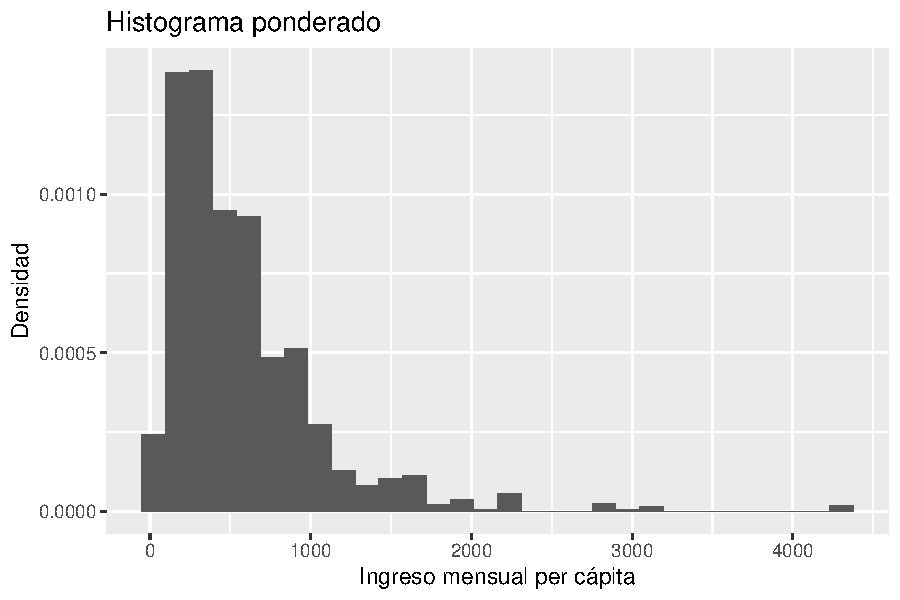
\includegraphics[width=0.65\linewidth,height=\textheight,keepaspectratio]{chapters/../figures/fig-hist-income-weighted-1.pdf}

}

\caption{\label{fig-hist-income-weighted}Histograma ponderado del
ingreso per cápita}

\end{figure}%

En este código, se inicia la construcción del gráfico utilizando la base
de datos \texttt{survey\_data}. Dentro de \texttt{aes()}, el argumento
\texttt{x\ =\ Income} indica que la variable representada en el eje
horizontal corresponde al ingreso, mientras que \texttt{weight\ =\ wk}
incorpora los pesos muestrales para construir un histograma ponderado
que refleje la distribución estimada en la población. La función
\texttt{geom\_histogram()} genera el histograma y, mediante
\texttt{aes(y\ =\ after\_stat(density))}, la altura de las barras se
expresa en términos de densidad en lugar de frecuencias absolutas. La
opción \texttt{bins\ =\ 30} fija el número de intervalos.
\texttt{labs()} identifica las unidades del eje horizontal y la densidad
del eje vertical; el área de las barras, y no su altura aislada,
representa proporciones. \texttt{ggtitle()} añade el título.

Para comparar la distribución del ingreso entre zonas urbanas y rurales,
se presenta un histograma ponderado en paneles separados y con escalas
comunes, como se muestra en la figura~\ref{fig-hist-zone}, obtenida con
el siguiente código computacional.

\begin{Shaded}
\begin{Highlighting}[]
\NormalTok{zone\_colors }\OtherTok{\textless{}{-}} \FunctionTok{c}\NormalTok{(}\AttributeTok{Urban =} \StringTok{"\#48C9B0"}\NormalTok{, }\AttributeTok{Rural =} \StringTok{"\#117864"}\NormalTok{)}

\NormalTok{weighted\_zone\_hist }\OtherTok{\textless{}{-}} \FunctionTok{ggplot}\NormalTok{(}
\NormalTok{  survey\_data,}
  \FunctionTok{aes}\NormalTok{(}\AttributeTok{x =}\NormalTok{ Income, }\AttributeTok{weight =}\NormalTok{ wk)}
\NormalTok{) }\SpecialCharTok{+}
  \FunctionTok{geom\_histogram}\NormalTok{(}
    \FunctionTok{aes}\NormalTok{(}\AttributeTok{y =} \FunctionTok{after\_stat}\NormalTok{(density)),}
    \AttributeTok{bins =} \DecValTok{30}\NormalTok{,}
    \AttributeTok{fill =} \StringTok{"\#48C9B0"}
\NormalTok{  ) }\SpecialCharTok{+}
  \FunctionTok{facet\_wrap}\NormalTok{(}
    \SpecialCharTok{\textasciitilde{}}\NormalTok{ Zone,}
    \AttributeTok{ncol =} \DecValTok{1}\NormalTok{,}
    \AttributeTok{labeller =} \FunctionTok{labeller}\NormalTok{(}\AttributeTok{Zone =} \FunctionTok{c}\NormalTok{(}\AttributeTok{Urban =} \StringTok{"Urbana"}\NormalTok{, }\AttributeTok{Rural =} \StringTok{"Rural"}\NormalTok{))}
\NormalTok{  ) }\SpecialCharTok{+}
  \FunctionTok{labs}\NormalTok{(}
    \AttributeTok{x =} \StringTok{"Ingreso mensual per cápita"}\NormalTok{,}
    \AttributeTok{y =} \StringTok{"Densidad"}\NormalTok{,}
    \AttributeTok{title =} \StringTok{"Distribución ponderada del ingreso por zona"}
\NormalTok{  )}

\NormalTok{weighted\_zone\_hist}
\end{Highlighting}
\end{Shaded}

\begin{figure}[H]

\centering{

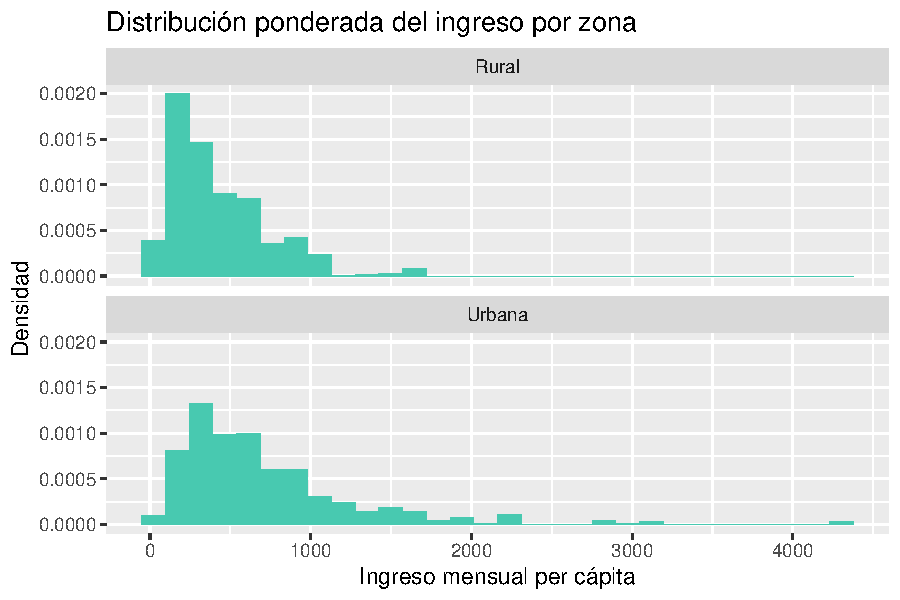
\includegraphics[width=0.65\linewidth,height=\textheight,keepaspectratio]{chapters/../figures/fig-hist-zone-1.pdf}

}

\caption{\label{fig-hist-zone}Histograma ponderado del ingreso por zona
geográfica}

\end{figure}%

Cada panel muestra la distribución ponderada del ingreso per cápita para
una zona. \texttt{facet\_wrap(\textasciitilde{}\ Zone,\ ncol\ =\ 1)}
separa las zonas en filas y conserva escalas comunes, de modo que las
alturas y los rangos del eje horizontal se puedan comparar directamente.
Las etiquetas de los paneles se presentan en español. Se utilizan los
mismos 30 intervalos en ambos paneles; el eje vertical muestra
densidades, por lo que el área de las barras representa proporciones.

Además, es posible superponer curvas de densidad suavizadas mediante la
función \texttt{geom\_density()}, lo que permite representar de manera
continua la forma de la distribución de la variable analizada. Este tipo
de gráfico facilita la identificación de características como la
asimetría, la concentración de los valores y la posible presencia de
múltiples modas. En la figura~\ref{fig-densities}, obtenida con el
siguiente código computacional, se presentan los histogramas del ingreso
y el gasto junto con sus respectivas curvas de densidad estimadas. Para
disponer ambos gráficos uno al lado del otro, se utiliza el operador
\texttt{\textbar{}} del paquete \texttt{patchwork}, que permite combinar
distintas visualizaciones en una misma composición gráfica.

\begin{Shaded}
\begin{Highlighting}[]
\NormalTok{weighted\_expenditure\_hist }\OtherTok{\textless{}{-}} \FunctionTok{ggplot}\NormalTok{(}
\NormalTok{  survey\_data,}
  \FunctionTok{aes}\NormalTok{(}\AttributeTok{x =}\NormalTok{ Expenditure, }\AttributeTok{weight =}\NormalTok{ wk)}
\NormalTok{) }\SpecialCharTok{+}
  \FunctionTok{geom\_histogram}\NormalTok{(}
    \FunctionTok{aes}\NormalTok{(}\AttributeTok{y =} \FunctionTok{after\_stat}\NormalTok{(density)),}
    \AttributeTok{bins =} \DecValTok{30}
\NormalTok{  ) }\SpecialCharTok{+}
  \FunctionTok{labs}\NormalTok{(}\AttributeTok{x =} \StringTok{"Gasto mensual per cápita"}\NormalTok{, }\AttributeTok{y =} \StringTok{"Densidad"}\NormalTok{)}

\NormalTok{(weighted\_income\_hist }\SpecialCharTok{+} \FunctionTok{geom\_density}\NormalTok{(}\AttributeTok{fill =} \StringTok{"blue"}\NormalTok{, }\AttributeTok{alpha =} \FloatTok{0.3}\NormalTok{)) }\SpecialCharTok{|}
\NormalTok{  (weighted\_expenditure\_hist }\SpecialCharTok{+} \FunctionTok{geom\_density}\NormalTok{(}\AttributeTok{fill =} \StringTok{"green"}\NormalTok{, }\AttributeTok{alpha =} \FloatTok{0.3}\NormalTok{))}
\end{Highlighting}
\end{Shaded}

\begin{figure}[H]

\centering{

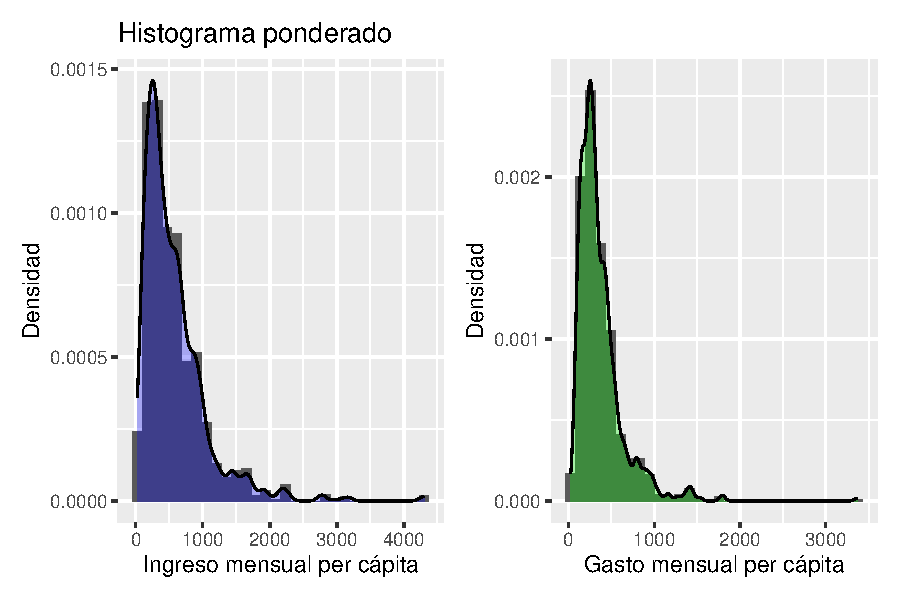
\includegraphics[width=0.9\linewidth,height=\textheight,keepaspectratio]{chapters/../figures/fig-densities-1.pdf}

}

\caption{\label{fig-densities}Histogramas ponderados y densidades del
ingreso y gasto per cápita}

\end{figure}%

\subsection{\texorpdfstring{Diagramas de caja
(\emph{boxplots})}{Diagramas de caja (boxplots)}}\label{diagramas-de-caja-boxplots}

Introducidos por Tukey (\citeproc{ref-Tukey1977EDA}{1977}), los
diagramas de caja (\emph{boxplots}) permiten identificar valores
atípicos y evaluar la dispersión de la distribución. Son una
representación gráfica que resume una variable mediante estadísticas
basadas en cuartiles, permitiendo identificar la mediana, la dispersión
de los datos y la presencia de valores atípicos. En el contexto de
encuestas de hogares, este tipo de gráfico resulta útil para comparar
distribuciones entre distintos grupos poblacionales de manera compacta y
visualmente intuitiva.

Los cuartiles y la mediana corresponden a los conceptos de la
Sección~\ref{sec-estimacion-de-percentiles}. Las cajas resumen la
dispersión y no son intervalos de confianza de la mediana. Para
incorporar las ponderaciones y el diseño muestral, se utiliza
\texttt{svyboxplot()} del paquete \texttt{survey}, que calcula y
representa diagramas de caja directamente a partir del objeto de diseño.
Como el ingreso y el gasto presentan asimetría y valores altos, se
muestran en escala logarítmica: esta comprime la cola superior y
facilita comparar los valores centrales entre zonas. En esta escala, las
distancias representan cambios multiplicativos. La transformación
requiere valores positivos, condición que cumplen ambas variables en
esta base. Las fórmulas especifican la variable graficada a la izquierda
de \texttt{\textasciitilde{}} y el grupo de comparación a la derecha. El
argumento \texttt{design} especifica el diseño muestral,
\texttt{horizontal\ =\ TRUE} dispone las cajas horizontalmente y
\texttt{col} asigna un color a cada zona.
\texttt{par(mfrow\ =\ c(1,\ 2))} organiza los dos gráficos en una fila,
y \texttt{par(old\_par)} restaura la configuración gráfica anterior. El
siguiente código computacional genera la
figura~\ref{fig-boxplot-zone-sex}.

\begin{Shaded}
\begin{Highlighting}[]
\NormalTok{survey\_design\_log }\OtherTok{\textless{}{-}}\NormalTok{ survey\_design }\SpecialCharTok{\%\textgreater{}\%}
  \FunctionTok{mutate}\NormalTok{(}
    \AttributeTok{log\_Income =} \FunctionTok{log}\NormalTok{(Income),}
    \AttributeTok{log\_Expenditure =} \FunctionTok{log}\NormalTok{(Expenditure)}
\NormalTok{  )}

\NormalTok{old\_par }\OtherTok{\textless{}{-}} \FunctionTok{par}\NormalTok{(}\AttributeTok{no.readonly =} \ConstantTok{TRUE}\NormalTok{)}
\FunctionTok{par}\NormalTok{(}\AttributeTok{mfrow =} \FunctionTok{c}\NormalTok{(}\DecValTok{1}\NormalTok{, }\DecValTok{2}\NormalTok{))}

\FunctionTok{svyboxplot}\NormalTok{(}
\NormalTok{  log\_Income }\SpecialCharTok{\textasciitilde{}}\NormalTok{ Zone,}
  \AttributeTok{design =}\NormalTok{ survey\_design\_log,}
  \AttributeTok{horizontal =} \ConstantTok{TRUE}\NormalTok{,}
  \AttributeTok{col =}\NormalTok{ zone\_colors,}
  \AttributeTok{xlab =} \StringTok{"Logaritmo del ingreso mensual per cápita"}\NormalTok{,}
  \AttributeTok{ylab =} \StringTok{"Zona"}\NormalTok{,}
  \AttributeTok{main =} \StringTok{"Ingreso por zona"}
\NormalTok{)}

\FunctionTok{svyboxplot}\NormalTok{(}
\NormalTok{  log\_Expenditure }\SpecialCharTok{\textasciitilde{}}\NormalTok{ Zone,}
  \AttributeTok{design =}\NormalTok{ survey\_design\_log,}
  \AttributeTok{horizontal =} \ConstantTok{TRUE}\NormalTok{,}
  \AttributeTok{col =}\NormalTok{ zone\_colors,}
  \AttributeTok{xlab =} \StringTok{"Logaritmo del gasto mensual per cápita"}\NormalTok{,}
  \AttributeTok{ylab =} \StringTok{"Zona"}\NormalTok{,}
  \AttributeTok{main =} \StringTok{"Gasto por zona"}
\NormalTok{)}

\FunctionTok{par}\NormalTok{(old\_par)}
\end{Highlighting}
\end{Shaded}

\begin{figure}[H]

\centering{

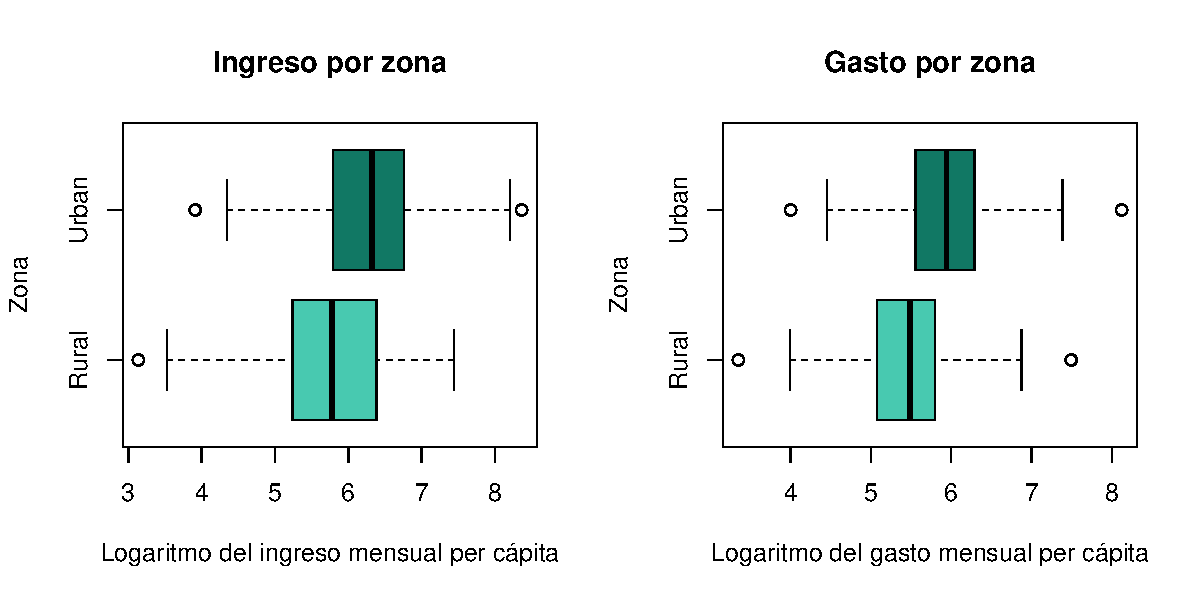
\includegraphics[width=0.9\linewidth,height=\textheight,keepaspectratio]{chapters/../figures/fig-boxplot-zone-sex-1.pdf}

}

\caption{\label{fig-boxplot-zone-sex}Cuartiles ponderados del logaritmo
del ingreso y el gasto per cápita por zona}

\end{figure}%

La figura~\ref{fig-boxplot-zone-sex} compara las distribuciones del
ingreso y el gasto per cápita en escala logarítmica entre las zonas
urbana y rural. Los bigotes se extienden hasta los valores observados
más extremos que quedan dentro de 1,5 rangos intercuartílicos; con el
valor predeterminado de \texttt{all.outliers\ =\ FALSE}, solo se
muestran como puntos los extremos más alejados. Las diferencias entre
medianas y cajas se interpretan en escala logarítmica y reflejan cambios
relativos, no diferencias absolutas en dólares.

\subsection{Diagramas de dispersión}\label{diagramas-de-dispersion}

Los diagramas de dispersión permiten examinar la relación entre dos
variables numéricas. En esta sección se compara el ingreso con el gasto
mensual per cápita. Ambas variables presentan distribuciones asimétricas
y valores altos, por lo que se representan en escala logarítmica: esta
comprime los valores extremos y facilita apreciar la concentración y los
patrones de asociación. Como las dos variables son positivas en esta
base, es posible aplicar esta transformación; en esa escala, las
distancias expresan cambios multiplicativos y no diferencias absolutas.
En el primer gráfico, el tamaño de cada punto representa el peso
muestral de la observación, lo que ayuda a explorar cuánta población
representa. Esta codificación visual no sustituye el ajuste de un modelo
ni incorpora por sí misma la incertidumbre del diseño. El siguiente
código computacional construye la figura~\ref{fig-scatter-basic}.

\begin{Shaded}
\begin{Highlighting}[]
\NormalTok{weighted\_basic\_scatter }\OtherTok{\textless{}{-}} \FunctionTok{ggplot}\NormalTok{(}
  \AttributeTok{data =}\NormalTok{ survey\_data,}
  \FunctionTok{aes}\NormalTok{(}\AttributeTok{y =}\NormalTok{ Income, }\AttributeTok{x =}\NormalTok{ Expenditure)}
\NormalTok{) }\SpecialCharTok{+}
  \FunctionTok{geom\_point}\NormalTok{(}\FunctionTok{aes}\NormalTok{(}\AttributeTok{size =}\NormalTok{ wk), }\AttributeTok{alpha =} \FloatTok{0.3}\NormalTok{) }\SpecialCharTok{+}
  \FunctionTok{scale\_x\_log10}\NormalTok{() }\SpecialCharTok{+}
  \FunctionTok{scale\_y\_log10}\NormalTok{() }\SpecialCharTok{+}
  \FunctionTok{labs}\NormalTok{(}
    \AttributeTok{x =} \StringTok{"Gasto mensual per cápita (escala log10)"}\NormalTok{,}
    \AttributeTok{y =} \StringTok{"Ingreso mensual per cápita (escala log10)"}
\NormalTok{  )}

\NormalTok{weighted\_basic\_scatter}
\end{Highlighting}
\end{Shaded}

\begin{figure}[H]

\centering{

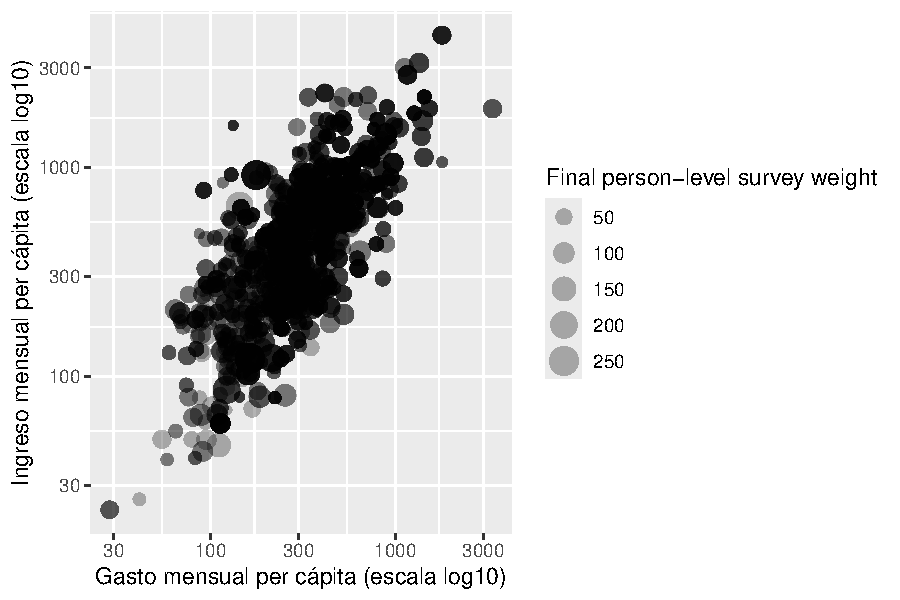
\includegraphics[width=0.65\linewidth,height=\textheight,keepaspectratio]{chapters/../figures/fig-scatter-basic-1.pdf}

}

\caption{\label{fig-scatter-basic}Diagrama de dispersión entre ingreso y
gasto per cápita}

\end{figure}%

La transparencia, fijada en 0,3 para todas las observaciones, facilita
la lectura de las zonas con mayor concentración de puntos.

Adicionalmente, es posible incorporar variables de agrupamiento en los
diagramas de dispersión mediante los argumentos \texttt{shape} y
\texttt{color}, los cuales permiten diferenciar visualmente las
observaciones según categorías específicas de la población. Esto
facilita la identificación de patrones diferenciados entre grupos y
mejora la interpretación de la relación entre las variables analizadas.
Un ejemplo de este tipo de representación se presenta en la
figura~\ref{fig-scatter-zone}, obtenida con el siguiente código
computacional.

\begin{Shaded}
\begin{Highlighting}[]
\NormalTok{weighted\_zone\_scatter }\OtherTok{\textless{}{-}} \FunctionTok{ggplot}\NormalTok{(}
  \AttributeTok{data =}\NormalTok{ survey\_data,}
  \FunctionTok{aes}\NormalTok{(}\AttributeTok{y =}\NormalTok{ Income, }\AttributeTok{x =}\NormalTok{ Expenditure, }\AttributeTok{shape =}\NormalTok{ Zone)}
\NormalTok{) }\SpecialCharTok{+}
  \FunctionTok{geom\_point}\NormalTok{(}\FunctionTok{aes}\NormalTok{(}\AttributeTok{size =}\NormalTok{ wk, }\AttributeTok{color =}\NormalTok{ Zone), }\AttributeTok{alpha =} \FloatTok{0.3}\NormalTok{) }\SpecialCharTok{+}
  \FunctionTok{labs}\NormalTok{(}
    \AttributeTok{size =} \StringTok{"Peso"}\NormalTok{,}
    \AttributeTok{x =} \StringTok{"Gasto mensual per cápita (escala log10)"}\NormalTok{,}
    \AttributeTok{y =} \StringTok{"Ingreso mensual per cápita (escala log10)"}
\NormalTok{  ) }\SpecialCharTok{+}
  \FunctionTok{scale\_color\_manual}\NormalTok{(}\AttributeTok{values =}\NormalTok{ zone\_colors) }\SpecialCharTok{+}
  \FunctionTok{scale\_x\_log10}\NormalTok{() }\SpecialCharTok{+}
  \FunctionTok{scale\_y\_log10}\NormalTok{()}

\NormalTok{weighted\_zone\_scatter}
\end{Highlighting}
\end{Shaded}

\begin{figure}[H]

\centering{

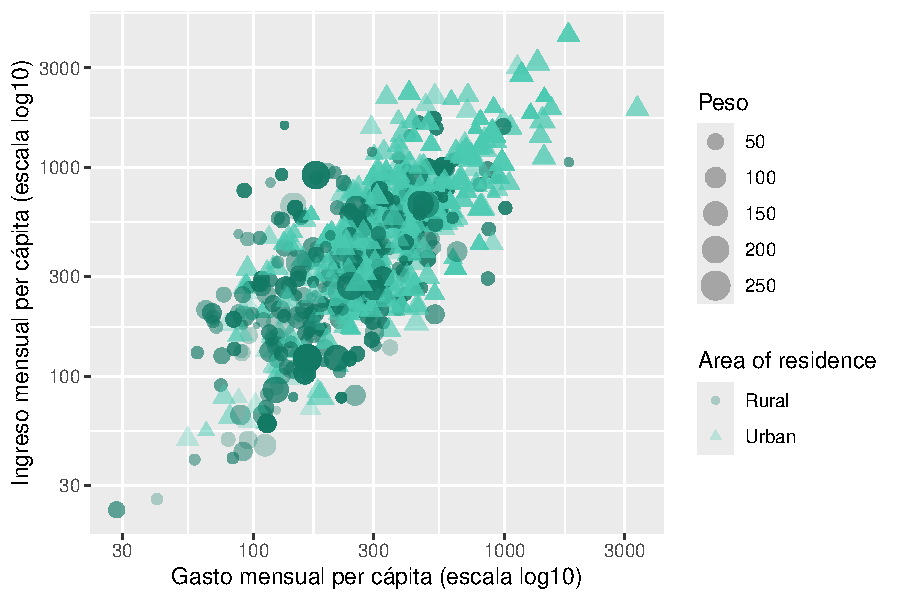
\includegraphics[width=0.65\linewidth,height=\textheight,keepaspectratio]{chapters/../figures/fig-scatter-zone-1.pdf}

}

\caption{\label{fig-scatter-zone}Diagrama de dispersión entre ingreso y
gasto por zona geográfica}

\end{figure}%

La figura~\ref{fig-scatter-zone} mantiene las mismas escalas
logarítmicas del gráfico anterior y diferencia las zonas por color y
forma. Así se pueden comparar los patrones entre zonas sin que los
valores altos compriman la mayor parte de los puntos. La escala
logarítmica cambia la lectura de los ejes: por ejemplo, un mismo tramo
visual corresponde a una razón constante entre valores, no a una
diferencia fija en dólares.

Las distribuciones y la correlación permiten reconocer heterogeneidad y
patrones de asociación. Junto con las herramientas para variables
categóricas, preparan el estudio de modelos de regresión del capítulo
siguiente, donde se analizarán varias variables simultáneamente
incorporando el diseño muestral.

\bookmarksetup{startatroot}

\chapter{Modelos de regresión}\label{cap5}

Los modelos de regresión constituyen una de las herramientas más
utilizadas en el análisis de datos provenientes de encuestas, ya que
permiten estudiar la relación entre una variable de interés y un
conjunto de variables explicativas
(\citeproc{ref-ChambersSkinner2003}{Chambers y Skinner 2003};
\citeproc{ref-HeeringaWestBerglund2017}{Heeringa et~al. 2017}). A través
de estos modelos, es posible evaluar cómo cambian determinadas
características de la población según factores demográficos, sociales o
económicos observados en la muestra. No obstante, la validez de los
resultados obtenidos depende de una adecuada especificación del modelo y
de la correcta consideración de las características del diseño muestral
de la encuesta.

En términos generales, los modelos de regresión buscan describir y
cuantificar la asociación entre una variable respuesta (dependiente) y
una o más variables explicativas (independientes), proporcionando
elementos para la interpretación estadística y la formulación de
inferencias sobre la población de estudio.

Por ejemplo, es posible analizar el comportamiento del gasto per cápita
de los hogares como variable de respuesta, en función del ingreso per
cápita, la edad y el sexo del jefe de hogar, la zona y la región de
residencia, consideradas variables explicativas. Utilizando información
proveniente de encuestas de hogares, este tipo de modelos permite
identificar patrones de asociación, cuantificar la asociación de
distintos factores socioeconómicos con el gasto y generar evidencia
empírica útil para el diseño, seguimiento y evaluación de políticas
públicas.

Como explica Pfeffermann
(\citeproc{ref-pfeffermann2011modelling}{2011}), dado que las encuestas
de hogares están sustentadas en diseños de muestreo complejos, los
métodos clásicos de regresión, desarrollados bajo supuestos de muestreo
aleatorio simple, pueden resultar inapropiados. Ignorar el diseño puede
sesgar los coeficientes cuando la selección es informativa o el modelo
está mal especificado y, aun cuando los coeficientes no cambien de
manera apreciable, puede producir errores estándar y pruebas de
hipótesis incorrectos.

En consecuencia, el análisis de datos provenientes de encuestas exige
una atención detallada al diseño de muestreo. La incorporación de los
pesos de la encuesta y los ajustes correspondientes a la estratificación
y la conglomeración permite obtener inferencias válidas y precisas.
Adicionalmente, en algunos casos se han propuesto alternativas
simplificadas, como el uso de pesos normalizados o enfoques de
ponderación aproximada, que buscan equilibrar la complejidad
metodológica con la factibilidad práctica del análisis.

El estudio de la regresión bajo diseños de muestreo complejos cuenta con
una trayectoria bien documentada. Como señalaron Kish y Frankel
(\citeproc{ref-kish1974inference}{1974}), estos diseños afectan las
inferencias derivadas de modelos de regresión. Posteriormente, Fuller
(\citeproc{ref-fuller1975regression}{1975}) desarrolló estimadores de
varianza apoyados en técnicas de linealización para modelos de regresión
lineal múltiple con ponderación desigual y métodos específicos para
diseños estratificados y de dos etapas.

Más adelante, Shah et~al. (\citeproc{ref-shah1977inference}{1977}) y
Binder (\citeproc{ref-binder1983variances}{1983}) abordaron el problema
de las violaciones a los supuestos clásicos al trabajar con datos de
encuestas mediante alternativas de inferencia robusta para los
parámetros. En paralelo, las distribuciones muestrales de los
estimadores de regresión en poblaciones finitas se incorporaron a
procedimientos para estimar varianzas bajo esquemas complejos.

En los años siguientes, Skinner et~al.
(\citeproc{ref-skinner1989analysis}{1989}) y Fuller
(\citeproc{ref-fuller2002regression}{2002}) ampliaron estos aportes
mediante estimadores de varianza para los coeficientes de regresión que
incorporan la estratificación y la conglomeración, así como mediante
compendios de métodos de estimación aplicables a modelos de regresión en
encuestas complejas. La discusión reciente incluye, además, métodos de
ponderación \emph{q-weighted} y evidencia empírica sobre su utilidad.

\section{Formulación del modelo}\label{formulacion-del-modelo}

Los modelos de regresión bajo diseños de muestreo complejos permiten
trascender las estadísticas descriptivas y estudiar asociaciones o
realizar predicciones. Su correcta aplicación abre la posibilidad de
examinar cómo las características sociodemográficas y económicas se
asocian con distintos resultados de interés, aportando evidencia clave
para la formulación de políticas públicas. Como explican Fox y Weisberg
(\citeproc{ref-FoxWeisberg2019}{2019}), la formulación más básica
corresponde al modelo de regresión lineal simple, el cual describe la
relación entre una variable respuesta y una única variable explicativa
mediante la siguiente expresión:

\[
y = \beta_{0} + \beta_{1}x + \varepsilon
\]

En donde \(y\) representa la variable de respuesta (dependiente), \(x\)
la variable explicativa (independiente), \(\beta_{0}\) el intercepto del
modelo, \(\beta_{1}\) el coeficiente asociado a la variable
independiente y \(\varepsilon\) el término de error, que recoge la
variabilidad no explicada por el modelo y puede interpretarse como la
diferencia entre el valor observado y el valor estimado por el modelo,
denotado por \(\hat{y}_k\).

En muchas aplicaciones empíricas, y especialmente en el análisis de
encuestas de hogares, el fenómeno de interés depende simultáneamente de
múltiples factores (\citeproc{ref-HeeringaWestBerglund2017}{Heeringa
et~al. 2017}). En estos casos se emplean modelos de regresión lineal
múltiple, los cuales incorporan varias variables explicativas:

\[
y = \beta_{0} + \beta_{1}x_{1} + \cdots + \beta_{p}x_{p} + \varepsilon,
\]

donde cada coeficiente \(\beta_{j}\) cuantifica la asociación entre la
variable respuesta y la correspondiente covariable \(x_{j}\),
manteniendo constantes las demás variables incluidas en el modelo. De
manera más compacta, el modelo puede expresarse utilizando notación
matricial como:

\begin{equation}\protect\phantomsection\label{eq-regresion-lineal-matricial}{
y_{k} = \mathbf{x}_{k}\boldsymbol{\beta} + \varepsilon_{k}, \quad k=1,\ldots,n,
}\end{equation}

donde \(\mathbf{x}_{k} = [1, x_{1k}, \ldots, x_{pk}]\) representa el
vector de covariables asociado a la unidad \(k\), mientras que
\(\boldsymbol{\beta} = [\beta_{0}, \beta_{1}, \ldots, \beta_{p}]'\)
corresponde al vector de parámetros desconocidos. Los modelos de
regresión lineal se sustentan en una serie de supuestos teóricos que
garantizan la validez de las estimaciones y de las inferencias derivadas
del modelo. En primer lugar, se asume que el valor esperado de los
residuos condicionado a las covariables es igual a cero, es decir,
\(E(\varepsilon_{k} \mid \mathbf{x}_{k}) = 0\), lo que implica la
ausencia de sesgos sistemáticos en la estimación de la variable
respuesta. Asimismo, se supone homogeneidad de la varianza de los
errores, de modo que la variabilidad residual permanece constante para
todos los valores de las covariables, esto es,
\(Var(\varepsilon_{k} \mid \mathbf{x}_{k}) = \sigma^2\). Adicionalmente,
se considera que los errores siguen una distribución normal con media
cero y varianza constante, expresada como
\(\varepsilon_{k} \mid \mathbf{x}_{k} \sim N(0,\sigma^2)\), y que los
residuos asociados a distintas observaciones son independientes entre
sí, de manera que
\(Cov(\varepsilon_{k},\varepsilon_{j}\mid \mathbf{x}_{k},\mathbf{x}_{j})=0\).

En este contexto, el valor esperado de la variable respuesta
condicionado al conjunto de covariables puede expresarse como:

\[
E(y \mid \mathbf{x}) = {\beta}_{0} + {\beta}_{1}x_{1} + \cdots + {\beta}_{p}x_{p}
\]

Los supuestos anteriores corresponden al modelo lineal clásico con
errores normales, independientes y de varianza constante. En el análisis
de encuestas complejas, la estimación de la incertidumbre incorpora las
características del diseño muestral, como se desarrolla a continuación.
Por ello, conviene distinguir los supuestos sobre la relación media
entre las variables de los utilizados para calcular los errores estándar
(\citeproc{ref-ChambersSkinner2003}{Chambers y Skinner 2003}).

\section{Uso de los pesos de
muestreo}\label{uso-de-los-pesos-de-muestreo}

Cuando se trabaja con datos provenientes de encuestas basadas en diseños
muestrales complejos, los supuestos clásicos de los modelos de regresión
rara vez se cumplen de manera estricta, puesto que las observaciones no
provienen de muestras aleatorias simples e independientes, sino de
esquemas de selección que incorporan elementos como estratificación,
conglomeración y probabilidades desiguales de selección. Por ejemplo, la
presencia de conglomeración puede violar el supuesto de independencia de
los errores, ya que individuos pertenecientes a un mismo hogar, segmento
o área geográfica tienden a compartir características similares. Del
mismo modo, las probabilidades desiguales de selección y los ajustes de
ponderación pueden generar heterogeneidad en la varianza de las
observaciones, incumpliendo el supuesto de homocedasticidad.

En este contexto, surge una pregunta fundamental: ¿de qué manera deben
incorporarse los pesos muestrales en los modelos de regresión? La
respuesta no es sencilla, ya que los pesos de la encuesta reflejan no
solo las probabilidades de selección, sino también diversos ajustes
asociados a la no respuesta, calibración y correcciones de cobertura.
Aunque su utilización permite producir estimaciones representativas de
la población, la incorporación directa de ponderaciones en los modelos
también puede reducir la eficiencia estadística e incrementar la
variabilidad de los estimadores.

En términos generales, Pfeffermann
(\citeproc{ref-pfeffermann2011modelling}{2011}) distingue dos enfoques
principales para abordar este problema. El primero corresponde al
enfoque basado en el diseño muestral, cuyo objetivo es obtener
inferencias válidas para la población objetivo respetando las
características del proceso de selección de la muestra. De acuerdo con
Heeringa et~al. (\citeproc{ref-HeeringaWestBerglund2017}{2017}), desde
esta perspectiva, los pesos muestrales son esenciales para corregir las
probabilidades desiguales de inclusión y producir estimaciones
insesgadas de los coeficientes de regresión. Sin embargo, este enfoque
no protege frente a posibles errores de especificación del modelo; es
decir, aun cuando las estimaciones sean válidas desde el punto de vista
del diseño, el modelo puede no representar adecuadamente las relaciones
existentes en la población.

El segundo corresponde al enfoque orientado al modelo, según el cual los
pesos no son necesariamente requeridos siempre que el modelo esté
correctamente especificado y el mecanismo de muestreo sea no
informativo. Bajo este supuesto, las relaciones entre las variables
observadas en la muestra coinciden con las de la población, de manera
que el diseño muestral no introduce sesgos relevantes en la estimación
de los parámetros. Desde esta perspectiva, incorporar ponderaciones
podría incluso resultar contraproducente, al aumentar innecesariamente
la varianza de los estimadores y, en consecuencia, los errores estándar.

Según Skinner et~al. (\citeproc{ref-skinner1989analysis}{1989}), la
discusión sobre la conveniencia de utilizar ponderaciones en modelos de
regresión ha sido ampliamente desarrollada en la literatura
especializada. En la práctica, una recomendación metodológica frecuente
consiste en estimar los modelos tanto con ponderaciones como sin ellas y
comparar posteriormente los resultados obtenidos
(\citeproc{ref-UNhandbook}{Naciones Unidas 2026}). Si la inclusión de
los pesos produce cambios importantes en los coeficientes estimados o
modifica las conclusiones sustantivas del análisis, ello sugiere que el
diseño de muestreo es informativo o que el modelo presenta problemas de
especificación, por lo que el uso de ponderaciones resulta aconsejable.
La comparación entre ajustes ponderados y no ponderados constituye un
diagnóstico, pero la estabilidad de los coeficientes no basta para
justificar la omisión de los pesos. Esa decisión requiere considerar el
objetivo inferencial, la especificación del modelo y el mecanismo de
selección de la muestra. Asimismo, debe distinguirse la decisión de
ponderar los coeficientes del tratamiento de la estratificación y la
conglomeración al estimar su incertidumbre.

En términos aplicados, esta decisión suele depender del propósito
analítico del estudio. Cuando el objetivo es realizar inferencia
descriptiva y producir estimaciones representativas de la población, la
utilización de ponderaciones es indispensable. En cambio, en contextos
de inferencia analítica orientados al estudio de asociaciones,
relaciones causales o contrastes de hipótesis, pueden emplearse tanto
modelos ponderados como no ponderados, especialmente cuando el modelo
incorpora variables relacionadas con el diseño muestral, como estratos o
conglomerados. No obstante, el uso de modelos no ponderados debe
justificarse cuidadosamente, dado que implica asumir condiciones más
restrictivas sobre el mecanismo de selección de la muestra y la correcta
especificación del modelo estadístico.

En resumen, cuando se opta por ponderar, las ponderaciones corrigen
posibles sesgos de sobre o subrepresentación de determinados grupos y
contribuyen a obtener estimaciones de varianza más exactas. Dentro del
enfoque basado en el diseño, esto permite que los resultados se
aproximen a valores insesgados comparables a los que se obtendrían en un
censo completo, incluso cuando el modelo no esté formulado de manera
óptima. Sin embargo, cuando los pesos presentan gran dispersión, pueden
aumentar la varianza de los parámetros estimados y volver inestables las
estimaciones, razón por la que en contextos explicativos o analíticos
los modelos sin ponderar pueden, en ocasiones, arrojar resultados más
consistentes y eficientes.

La selección adecuada de las variables explicativas y la consideración
del mecanismo de selección de la muestra son fundamentales para el
análisis. Además de estas decisiones, algunas implementaciones utilizan
versiones reescaladas de los pesos originales. A continuación, se
presentan dos formas habituales de reescalamiento, que modifican la suma
de los pesos, pero no corrigen una especificación incorrecta del modelo
ni reducen la dispersión relativa de las ponderaciones:

\begin{enumerate}
\def\labelenumi{\arabic{enumi}.}
\item
  Pesos tipo Senado: este procedimiento ajusta los pesos de manera que
  su suma coincida con el tamaño de la muestra, en lugar del tamaño de
  la población. Esta transformación multiplica todos los pesos por una
  constante y conserva su dispersión relativa; por tanto, no constituye
  un recorte de pesos extremos. Las nuevas ponderaciones son
  \(w_k^{Senate} = w_k \times \frac{n}{\sum w_k}\).
\item
  Pesos normalizados: en este enfoque los pesos originales se reescalan
  para que su suma sea igual a uno. Al ser también una multiplicación
  por una constante común, el reescalamiento no reduce por sí mismo la
  variabilidad relativa de los pesos ni sustituye la especificación del
  diseño; su efecto sobre las varianzas depende del método y del
  software utilizados. Las nuevas ponderaciones son
  \(w_k^{Normalized} = \frac{w_k}{\sum w_k}\).
\end{enumerate}

Es importante destacar que, en ambos métodos, los pesos ajustados se
obtienen mediante transformaciones multiplicativas directas de los pesos
muestrales originales. Por ello, no deben emplearse para calcular
tamaños o totales poblacionales. Asimismo, estos procedimientos no
alteran las estimaciones de razones, como medias o proporciones, ya que
en tales casos los pesos se cancelan en el cociente. En la práctica, el
uso de estos ajustes puede considerarse una solución pragmática en
contextos donde no se dispone de software especializado para encuestas.
No obstante, cuando se cuenta con herramientas como los paquetes
\texttt{survey} y \texttt{srvyr} en \texttt{R}, descritos en los
capítulos anteriores, el reescalamiento deja de ser necesario, pues
dichos paquetes realizan el tratamiento adecuado para preservar tanto la
representatividad como las propiedades inferenciales del modelo.

\section{Estimación de los parámetros del
modelo}\label{estimacion-de-los-parametros-del-modelo}

De acuerdo con Molina y Skinner (\citeproc{ref-molina1992pseudo}{1992})
y Binder (\citeproc{ref-binder2011estimating}{2011}), en términos del
ajuste de modelos de regresión con encuestas de hogares, se han
desarrollado metodologías inferenciales avanzadas que integran las
fuentes de incertidumbre en un mismo marco analítico, buscando reflejar
tanto la estructura del diseño como los supuestos y limitaciones del
modelo. Entre las aproximaciones más relevantes se encuentran la
pseudo-verosimilitud y la inferencia combinada.

El método de pseudo-verosimilitud extiende las técnicas tradicionales de
máxima verosimilitud para ajustarlas a las particularidades de los
diseños muestrales complejos. En este enfoque, la distribución de
muestreo definida por el diseño ocupa un rol central, mientras que la
distribución del modelo pasa a un segundo plano. Si bien en contextos de
modelos bien especificados los estimadores basados en
pseudo-verosimilitud tienden a ser insesgados o consistentes, su
principal virtud radica en evitar los sesgos que se originarían al
ignorar el diseño muestral. En términos prácticos, este método traduce
el modelo tradicional en uno que respeta la forma en que los datos
fueron obtenidos, garantizando inferencias más sólidas.

En contraste, la inferencia combinada propone un marco unificado en el
que se integran simultáneamente la variabilidad del muestreo y la
incertidumbre del modelo. Considerar ambas fuentes permite caracterizar
de manera más completa la variabilidad total, aunque sus propiedades
dependen del diseño y de la especificación del modelo. Un desarrollo
teórico más detallado de este enfoque, acompañado de simulaciones
computacionales, se presenta en el \hyperref[ap2]{segundo anexo}.

Además, tal como explica Wolter
(\citeproc{ref-Wolter2007Variance}{2007}), cuando se desea estimar los
parámetros de un modelo de regresión lineal a partir de una muestra con
un diseño complejo, el enfoque estándar cambia. En consecuencia, los
estimadores tradicionales, como los obtenidos por máxima verosimilitud o
mínimos cuadrados, pueden resultar sesgados y producir errores estándar
poco confiables. Frente a esta situación, los métodos de estimación de
varianza, como la linealización de Taylor y el bootstrap, son válidos en
la medida en que su implementación reproduzca las características
pertinentes del diseño.

Según Fuller (\citeproc{ref-fuller2002regression}{2002}) y Chambers y
Skinner (\citeproc{ref-ChambersSkinner2003}{2003}), en el caso de un
modelo de regresión lineal simple, la estimación de \(\beta_1\) bajo un
esquema de muestreo complejo se realiza, mediante un estimador
ponderado, que puede expresarse de la siguiente forma:

\begin{equation}\protect\phantomsection\label{eq-pendiente-ponderada}{
\hat{\beta_{1}}  =
\frac{\sum_{h} \sum_{i} \sum_{k} w_{hik}\,(y_{hik}-\hat{\bar{y}})(x_{hik}-\hat{\bar{x}})}
{\sum_{h} \sum_{i} \sum_{k} w_{hik}\,(x_{hik}-\hat{\bar{x}})^{2}}
=
\frac{\hat{t}_{xy}}{\hat{t}_{xx}}
}\end{equation}

En donde \(\hat{\bar{y}}=\hat{t}_y/\hat{N}\) y
\(\hat{\bar{x}}=\hat{t}_x/\hat{N}\) corresponden a las medias estimadas
de las variables de estudio y auxiliar, respectivamente, mientras que
\(w_{hik}\) representa los pesos de muestreo asociados a cada unidad de
observación. Esta formulación incorpora explícitamente dichos pesos, lo
que permite considerar las probabilidades desiguales de selección y las
características propias del diseño muestral. Asimismo, la varianza
estimada de \(\hat{\beta}_1\) puede aproximarse como:

\begin{equation}\protect\phantomsection\label{eq-varianza-pendiente}{
\widehat{Var}\left(\hat{\beta_{1}}\right)
\approx  \frac{\widehat{Var}(\hat{t}_{xy})+\hat{\beta}_{1}^{2}\widehat{Var}(\hat{t}_{xx})-2\hat{\beta}_{1}\widehat{Cov}(\hat{t}_{xy},\hat{t}_{xx})}{(\hat{t}_{xx})^{2}}
}\end{equation}

Si \(\hat{\beta}_{1}\) corresponde al estimador de la pendiente en un
modelo de regresión lineal simple ponderado, entonces el estimador del
intercepto \(\hat{\beta}_{0}\) está dado por

\[
\hat{\beta}_{0} = \hat{\bar{y}} - \hat{\beta}_{1}\hat{\bar{x}}
\]

Nótese que la varianza de \(\hat{\beta}_{0}\) depende simultáneamente de
los estimadores \(\hat{\bar{y}}\), \(\hat{\bar{x}}\) y
\(\hat{\beta}_{1}\). Por esta razón, su aproximación puede obtenerse
mediante las propiedades de la varianza de combinaciones lineales de
estimadores, en conjunto con técnicas de linearización de Taylor. A
partir de este procedimiento se deriva la matriz de varianzas y
covarianzas de los coeficientes del modelo, de la cual se obtienen tanto
los errores estándar como las covarianzas asociadas a las estimaciones
de los parámetros.

De acuerdo con Kish y Frankel (\citeproc{ref-kish1974inference}{1974}),
en el caso de la regresión múltiple, si \(\hat{\boldsymbol{\beta}}\)
representa el estimador de \(\boldsymbol{\beta}\), entonces la varianza
de cada coeficiente se estima considerando su interdependencia con los
demás parámetros, lo que se refleja en la construcción de una matriz de
varianzas-covarianzas que recoge tanto la variabilidad individual como
las covarianzas entre todos los estimadores. Este cálculo requiere
utilizar totales ponderados de cuadrados y productos cruzados de todas
las combinaciones entre la variable dependiente \(y\) y el conjunto de
predictores \(\mathbf{x} = (1, x_1, \ldots, x_p)\). En términos
generales:

\[
\widehat{Var}(\hat{\boldsymbol{\beta}}) = \hat{\boldsymbol\Sigma} =
\begin{bmatrix}
\widehat{Var}(\hat{\beta}_{0}) & \widehat{Cov}(\hat{\beta}_{0},\hat{\beta}_{1}) & \cdots & \widehat{Cov}(\hat{\beta}_{0},\hat{\beta}_{p}) \\
\widehat{Cov}(\hat{\beta}_{0},\hat{\beta}_{1}) & \widehat{Var}(\hat{\beta}_{1}) & \cdots & \widehat{Cov}(\hat{\beta}_{1},\hat{\beta}_{p}) \\
\vdots & \vdots & \ddots & \vdots \\
\widehat{Cov}(\hat{\beta}_{0},\hat{\beta}_{p}) & \widehat{Cov}(\hat{\beta}_{1},\hat{\beta}_{p}) & \cdots & \widehat{Var}(\hat{\beta}_{p})
\end{bmatrix}
\]

En este capítulo se mostrará cómo implementar estos modelos en
\texttt{R} mediante las librerías \texttt{survey} y \texttt{srvyr},
junto con \texttt{tidyverse} para organizar el flujo de trabajo. Se
abordará la especificación del diseño muestral, la estimación de modelos
lineales, así como la obtención de errores estándar y pruebas de
hipótesis ajustadas al diseño, integrando los fundamentos teóricos con
ejemplos prácticos reproducibles. Para ejemplificar los conceptos
desarrollados hasta este punto, se empleará la misma base de datos
utilizada a lo largo del libro. El siguiente código computacional carga
los paquetes y los datos, prepara las variables categóricas y define el
diseño de muestreo que se utilizará en los modelos del capítulo.

\begin{Shaded}
\begin{Highlighting}[]
\FunctionTok{library}\NormalTok{(survey)}
\FunctionTok{library}\NormalTok{(srvyr)}
\FunctionTok{library}\NormalTok{(tidyverse)}

\FunctionTok{data}\NormalTok{(BigCity, }\AttributeTok{package =} \StringTok{"TeachingSampling"}\NormalTok{)}
\NormalTok{survey\_data }\OtherTok{\textless{}{-}} \FunctionTok{readRDS}\NormalTok{(}\StringTok{"../data/sample.rds"}\NormalTok{) }\SpecialCharTok{\%\textgreater{}\%}
  \FunctionTok{mutate}\NormalTok{(}
    \AttributeTok{Stratum =} \FunctionTok{factor}\NormalTok{(Stratum),}
    \AttributeTok{Sex =} \FunctionTok{factor}\NormalTok{(Sex, }\AttributeTok{levels =} \FunctionTok{c}\NormalTok{(}\StringTok{"Male"}\NormalTok{, }\StringTok{"Female"}\NormalTok{)),}
    \AttributeTok{Zone =} \FunctionTok{factor}\NormalTok{(Zone, }\AttributeTok{levels =} \FunctionTok{c}\NormalTok{(}\StringTok{"Rural"}\NormalTok{, }\StringTok{"Urban"}\NormalTok{))}
\NormalTok{  )}

\NormalTok{survey\_design }\OtherTok{\textless{}{-}}\NormalTok{ survey\_data }\SpecialCharTok{\%\textgreater{}\%}
  \FunctionTok{as\_survey\_design}\NormalTok{(}
    \AttributeTok{strata =}\NormalTok{ Stratum,}
    \AttributeTok{ids =}\NormalTok{ PSU,}
    \AttributeTok{weights =}\NormalTok{ wk,}
    \AttributeTok{nest =} \ConstantTok{TRUE}
\NormalTok{  ) }\SpecialCharTok{\%\textgreater{}\%}
  \FunctionTok{filter}\NormalTok{(PersonID }\SpecialCharTok{==} \StringTok{"idPer01"}\NormalTok{, Income }\SpecialCharTok{\textgreater{}} \DecValTok{0}\NormalTok{, Expenditure }\SpecialCharTok{\textgreater{}} \DecValTok{0}\NormalTok{)}

\NormalTok{survey\_data }\OtherTok{\textless{}{-}}\NormalTok{ survey\_design}\SpecialCharTok{$}\NormalTok{variables}
\end{Highlighting}
\end{Shaded}

La base \texttt{sample.rds} conserva los nombres de las variables y
utiliza etiquetas y categorías en inglés. En \texttt{Region}, las
categorías \texttt{North}, \texttt{South}, \texttt{Central},
\texttt{West} y \texttt{East} corresponden a Norte, Sur, Centro,
Occidente y Oriente; \texttt{CatAge} contiene grupos decenales
ordenados: \texttt{0-9}, \texttt{10-19}, \texttt{20-29}, y así
sucesivamente hasta \texttt{90-99}.

En este capítulo se trabaja con una observación por hogar, identificada
mediante \texttt{PersonID\ ==\ "idPer01"}, y se utiliza el factor de
expansión \texttt{wk} del jefe, siguiendo la convención descrita en la
sección 3.1. La muestra de análisis contiene 696 hogares con ingreso y
gasto positivos, condición necesaria para calcular sus logaritmos
naturales. La edad y el sexo corresponden al jefe del hogar; las
categorías de referencia son hombre, zona rural y región Norte.

Con el objetivo de ajustar un modelo de regresión entre los logaritmos
del ingreso y del gasto per cápita, resulta conveniente explorar
previamente la relación existente entre ambas variables. Para ello, se
construye un diagrama de dispersión mediante \texttt{ggplot2}, el cual
permite evaluar visualmente la forma y la intensidad de la asociación.
El resultado se presenta en la
figura~\ref{fig-scatter-sample-unweighted}, obtenida con el siguiente
código computacional.

\begin{Shaded}
\begin{Highlighting}[]
\NormalTok{unweighted\_plot }\OtherTok{\textless{}{-}} \FunctionTok{ggplot}\NormalTok{(}
  \AttributeTok{data =}\NormalTok{ survey\_data,}
  \FunctionTok{aes}\NormalTok{(}\AttributeTok{x =} \FunctionTok{log}\NormalTok{(Income), }\AttributeTok{y =} \FunctionTok{log}\NormalTok{(Expenditure))}
\NormalTok{) }\SpecialCharTok{+}
  \FunctionTok{geom\_point}\NormalTok{() }\SpecialCharTok{+}
  \FunctionTok{geom\_smooth}\NormalTok{(}\AttributeTok{method =} \StringTok{"lm"}\NormalTok{, }\AttributeTok{se =} \ConstantTok{FALSE}\NormalTok{) }\SpecialCharTok{+}
  \FunctionTok{labs}\NormalTok{(}
    \AttributeTok{x =} \StringTok{"Logaritmo del ingreso per cápita"}\NormalTok{,}
    \AttributeTok{y =} \StringTok{"Logaritmo del gasto per cápita"}
\NormalTok{  )}

\NormalTok{unweighted\_plot}
\end{Highlighting}
\end{Shaded}

\begin{figure}[H]

\centering{

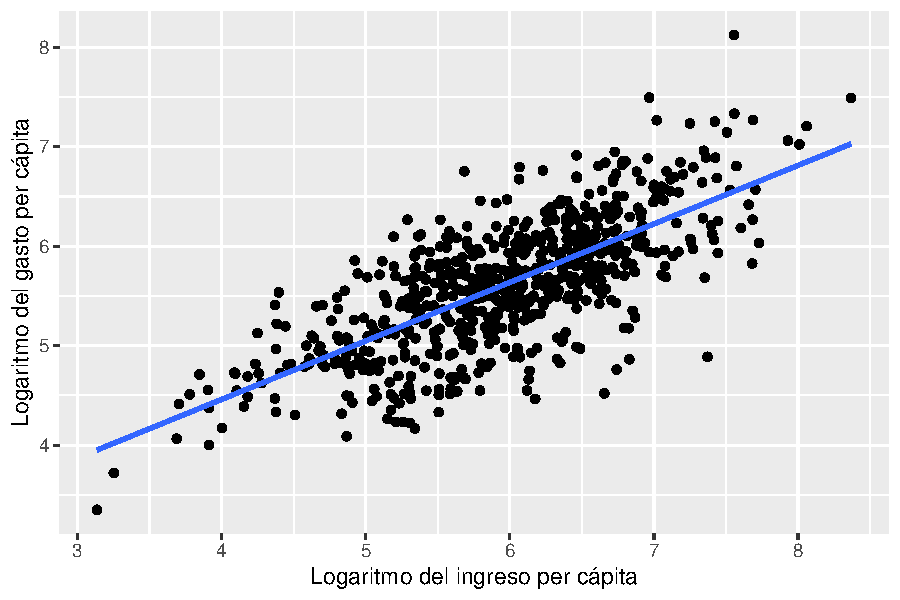
\includegraphics[width=0.65\linewidth,height=\textheight,keepaspectratio]{chapters/../figures/fig-scatter-sample-unweighted-1.pdf}

}

\caption{\label{fig-scatter-sample-unweighted}Diagrama de dispersión
entre los logaritmos del ingreso y del gasto per cápita de los hogares
(sin ponderar)}

\end{figure}%

Los datos muestrales conservan una relación positiva y aproximadamente
lineal entre los logaritmos del ingreso y del gasto per cápita, aunque
se observa dispersión alrededor de la recta ajustada. Una vez completada
la exploración gráfica de los datos, se procede al ajuste de los modelos
de regresión lineal.

El siguiente código computacional ajusta un modelo lineal mediante
\texttt{svyglm()} del paquete \texttt{survey}, incorporando los factores
de expansión y las demás características del diseño muestral. En este
caso, la expresión
\texttt{log(Expenditure)\ \textasciitilde{}\ log(Income)\ +\ Age\ +\ Sex\ +\ Zone\ +\ Region}
especifica que el logaritmo del gasto per cápita se modela en función
del logaritmo del ingreso per cápita, la edad y el sexo del jefe de
hogar, la zona y la región de residencia; es decir, se ajusta una
regresión lineal múltiple en escala logarítmica, cuyo coeficiente del
ingreso representa la elasticidad del gasto respecto al ingreso,
manteniendo constantes las demás variables. El argumento
\texttt{design\ =\ survey\_design} indica que el modelo debe utilizar el
objeto de diseño muestral previamente definido, mientras que
\texttt{family\ =\ stats::gaussian()} especifica que se ajusta un modelo
lineal con distribución normal, equivalente a una regresión lineal
clásica.

\begin{Shaded}
\begin{Highlighting}[]
\NormalTok{fit\_svy }\OtherTok{\textless{}{-}} \FunctionTok{svyglm}\NormalTok{(}
  \FunctionTok{log}\NormalTok{(Expenditure) }\SpecialCharTok{\textasciitilde{}} \FunctionTok{log}\NormalTok{(Income) }\SpecialCharTok{+}\NormalTok{ Age }\SpecialCharTok{+}\NormalTok{ Sex }\SpecialCharTok{+}\NormalTok{ Zone }\SpecialCharTok{+}\NormalTok{ Region,}
  \AttributeTok{design =}\NormalTok{ survey\_design,}
  \AttributeTok{family =}\NormalTok{ stats}\SpecialCharTok{::}\FunctionTok{gaussian}\NormalTok{()}
\NormalTok{)}

\NormalTok{fit\_svy}
\end{Highlighting}
\end{Shaded}

\begin{verbatim}
Stratified 1 - level Cluster Sampling design (with replacement)
With (238) clusters.
Called via srvyr
Sampling variables:
  - ids: PSU 
  - strata: Stratum 
  - weights: wk 

Call:  svyglm(formula = log(Expenditure) ~ log(Income) + Age + Sex + 
    Zone + Region, design = survey_design, family = stats::gaussian())

Coefficients:
  (Intercept)    log(Income)            Age      SexFemale      ZoneUrban  
      2.38093        0.53684       -0.00189        0.00287        0.14988  
  RegionSouth  RegionCentral     RegionWest     RegionEast  
      0.05829        0.21195        0.00762        0.00544  

Degrees of Freedom: 695 Total (i.e. Null);  111 Residual
Null Deviance:      293 
Residual Deviance: 128  AIC: NA
\end{verbatim}

La salida anterior corresponde al ajuste de un modelo de regresión
lineal en el que el logaritmo de \texttt{Expenditure} se explica a
partir del logaritmo de \texttt{Income} y de las variables \texttt{Age},
\texttt{Sex}, \texttt{Zone} y \texttt{Region}. Como explica Wooldridge
(\citeproc{ref-Wooldridge2020}{2020}), la interpretación de los
coeficientes depende de cuáles variables se expresan en logaritmos. En
este modelo, tanto el gasto como el ingreso per cápita están en
logaritmos, por lo que el coeficiente de \texttt{log(Income)} representa
directamente una elasticidad: un ingreso 1 \% mayor se asocia con un
gasto aproximadamente \(\hat\beta_1\) \% mayor, manteniendo constantes
las demás variables. En cambio, para la edad, incorporada en su escala
original, un año adicional se asocia con una variación porcentual de
\(100[\exp(\hat\beta_{\mathrm{Age}})-1]\). Para las variables
categóricas, esa misma transformación expresa la diferencia porcentual
respecto de la categoría de referencia. La exponencial convierte el
coeficiente en una razón entre niveles de gasto ajustados; restar uno y
multiplicar por cien permite expresar cuánto aumenta o disminuye el
gasto respecto del nivel de comparación.

Por lo tanto, los resultados indican la existencia de una relación
positiva entre ingreso y gasto, de modo que, manteniendo constantes las
demás variables, un ingreso per cápita 1 \% mayor se asocia con un gasto
per cápita aproximadamente 0.537 \% mayor. Asimismo, se evidencian
diferencias asociadas a las características sociodemográficas incluidas
en el modelo: residir en zona urbana se asocia con un gasto per cápita
aproximadamente 16.17 \% mayor que en zona rural, mientras que
pertenecer a un hogar con jefatura femenina se asocia con un gasto 0.29
\% mayor que con jefatura masculina. Cada año adicional de edad del jefe
se asocia con un gasto aproximadamente 0.19 \% menor. Respecto de la
región Norte, las diferencias estimadas son 6.00 \% para Sur, 23.61 \%
para Centro, 0.76 \% para Occidente y 0.55 \% para Oriente. Estas
diferencias se obtienen mediante \(100[\exp(\hat\beta_j)-1]\) y
describen asociaciones en la escala multiplicativa, sin establecer
efectos causales. El intercepto estimado, igual a 2.381, representa el
valor esperado del logaritmo del gasto para la categoría de referencia
del modelo cuando el ingreso per cápita es igual a uno y la edad es
cero; este perfil queda fuera del rango observado de edad de los jefes,
por lo que su interpretación es principalmente algebraica.

\section{Diagnóstico del modelo}\label{diagnostico-del-modelo}

De acuerdo con Fox y Weisberg (\citeproc{ref-FoxWeisberg2019}{2019}), en
el análisis de encuestas de hogares, la evaluación de un modelo
estadístico constituye un aspecto importante que contribuye a valorar la
validez de las inferencias. Un modelo adecuadamente especificado no
depende únicamente de la selección de las covariables, sino también del
examen de los supuestos que sustentan la consistencia y confiabilidad de
los resultados.

En el caso de los modelos de regresión lineal aplicados a encuestas
complejas, resulta necesario examinar distintos aspectos relacionados
con la calidad del ajuste y el comportamiento de los errores. Como se
indicó anteriormente, entre ellos se encuentran la capacidad explicativa
del modelo, la normalidad y homogeneidad de la varianza de los residuos,
la independencia entre errores y la posible presencia de observaciones
influyentes o valores atípicos que puedan afectar las estimaciones
(\citeproc{ref-Li_Valliant_2015}{Li y Valliant 2015}).

Estas verificaciones adquieren particular importancia en el contexto de
diseños muestrales complejos, donde características como la
estratificación, la conglomeración y el uso de factores de expansión
pueden intensificar problemas asociados con la heterocedasticidad, la
dependencia entre observaciones o la sensibilidad a valores extremos.
Por esta razón, el diagnóstico del modelo no debe limitarse a los
supuestos clásicos de la regresión, sino incorporar también las
particularidades derivadas del diseño de la encuesta. La aplicación
sistemática de estos procedimientos permite evaluar la solidez del
modelo, fortalecer la confianza en las inferencias y asegurar que los
resultados obtenidos sean representativos y útiles tanto para la
investigación social aplicada como para el análisis de políticas
públicas.

\subsection{Coeficiente de
determinación}\label{coeficiente-de-determinacion}

Una de las medidas más utilizadas para evaluar el ajuste de un modelo de
regresión es el coeficiente de determinación, denotado por \(R^{2}\).
Este indicador cuantifica la proporción de la variabilidad de la
variable dependiente que es explicada por el modelo
(\citeproc{ref-FoxWeisberg2019}{Fox y Weisberg 2019}). Sus valores
oscilan entre cero y uno: cuanto más cercano se encuentre a la unidad,
mayor será la capacidad explicativa del modelo; en contraste, valores
próximos a cero indican un bajo nivel de explicación de la variabilidad
observada. La magnitud del \(R^{2}\) no debe evaluarse en términos
absolutos, sino considerando el fenómeno estudiado y el tipo de
información disponible.

El coeficiente se calcula a partir de las sumas de cuadrados totales y
de error, como \(R^{2} = 1 - \frac{SSE}{SST}\); en donde \(SST\)
representa la suma de cuadrados totales y \(SSE\) la suma de cuadrados
del error. Según Heeringa et~al.
(\citeproc{ref-HeeringaWestBerglund2017}{2017}), en encuestas con
diseños de muestreo complejos, esta medida debe ajustarse para
incorporar la estructura del diseño y los pesos muestrales. El estimador
ponderado del coeficiente de determinación se define como:

\[
\hat{R}^2 = 1 - \frac{\widehat{SSE}}{\widehat{SST}}
\]

donde
\(\widehat{SSE} = \sum_{h} \sum_{i} \sum_{k} w_{hik} \,(y_{hik} - x_{hik}\hat{\boldsymbol{\beta}})^2\)
es la suma ponderada de errores al cuadrado; mientras que
\(\widehat{SST} = \sum_{h} \sum_{i} \sum_{k} w_{hik}\,(y_{hik} - \hat{\bar{y}})^2\)
representa la suma total ponderada de cuadrados.

De acuerdo con Pfeffermann
(\citeproc{ref-pfeffermann2011modelling}{2011}), dado que el \(R^{2}\)
tiende a incrementarse conforme se incorporan más variables al modelo,
conviene complementar su interpretación con el coeficiente de
determinación ajustado (\(R_{adj}^{2}\)), el cual introduce una
penalización en función del número de covariables incluidas y del tamaño
muestral. Este coeficiente se define como
\(\hat{R}^2_{adj} = 1 - \frac{(n-1)}{(n-p)}(1 - \hat{R}^2)\), donde
\(n\) corresponde al número de observaciones, \(p\) representa el número
de parámetros estimados y \(\hat{R}^{2}\) denota el coeficiente de
determinación ponderado definido previamente.

De esta manera, el ajuste permite evaluar la capacidad explicativa del
modelo controlando el efecto derivado de la incorporación de nuevas
variables. Este ajuste facilita una comparación más equitativa entre
modelos con distinto número de predictores y resulta particularmente
útil en el análisis de encuestas, donde la complejidad del diseño y el
uso de ponderaciones pueden influir notablemente en la magnitud del
\(R^{2}\).

El siguiente código computacional obtiene los componentes necesarios
para calcular el coeficiente de determinación \(R^{2}\). Para estimar la
suma total ponderada de cuadrados (\(\widehat{SST}\)), ajusta primero un
modelo nulo que incluye únicamente el intercepto.

\begin{Shaded}
\begin{Highlighting}[]
\NormalTok{null\_model }\OtherTok{\textless{}{-}} \FunctionTok{svyglm}\NormalTok{(}\FunctionTok{log}\NormalTok{(Expenditure) }\SpecialCharTok{\textasciitilde{}} \DecValTok{1}\NormalTok{, }\AttributeTok{design =}\NormalTok{ survey\_design)}

\NormalTok{s1 }\OtherTok{\textless{}{-}} \FunctionTok{summary}\NormalTok{(fit\_svy)}
\NormalTok{s0 }\OtherTok{\textless{}{-}} \FunctionTok{summary}\NormalTok{(null\_model)}

\NormalTok{wsst }\OtherTok{\textless{}{-}}\NormalTok{ s0}\SpecialCharTok{$}\NormalTok{dispersion[}\DecValTok{1}\NormalTok{]}
\NormalTok{wsse }\OtherTok{\textless{}{-}}\NormalTok{ s1}\SpecialCharTok{$}\NormalTok{dispersion[}\DecValTok{1}\NormalTok{]}
\end{Highlighting}
\end{Shaded}

La estimación del coeficiente de determinación y su contraparte ajustada
se obtiene a partir del siguiente cálculo:

\begin{Shaded}
\begin{Highlighting}[]
\NormalTok{n }\OtherTok{\textless{}{-}} \FunctionTok{nrow}\NormalTok{(survey\_design)}
\NormalTok{p }\OtherTok{\textless{}{-}} \FunctionTok{length}\NormalTok{(}\FunctionTok{coef}\NormalTok{(fit\_svy))}
\NormalTok{r2 }\OtherTok{\textless{}{-}} \DecValTok{1} \SpecialCharTok{{-}}\NormalTok{ wsse }\SpecialCharTok{/}\NormalTok{ wsst}
\NormalTok{r2\_adj }\OtherTok{\textless{}{-}} \DecValTok{1} \SpecialCharTok{{-}}\NormalTok{ ((n }\SpecialCharTok{{-}} \DecValTok{1}\NormalTok{) }\SpecialCharTok{/}\NormalTok{ (n }\SpecialCharTok{{-}}\NormalTok{ p)) }\SpecialCharTok{*}\NormalTok{ (}\DecValTok{1} \SpecialCharTok{{-}}\NormalTok{ r2)}

\NormalTok{r2}
\end{Highlighting}
\end{Shaded}

\begin{verbatim}
[1] 0.5645
\end{verbatim}

\begin{Shaded}
\begin{Highlighting}[]
\NormalTok{r2\_adj}
\end{Highlighting}
\end{Shaded}

\begin{verbatim}
[1] 0.5594
\end{verbatim}

Los resultados muestran un \(R^2\) de 0,5645 y un \(R^2\) ajustado de
0,5594. Estos coeficientes resumen la proporción de variabilidad del
logaritmo del gasto per cápita explicada por el conjunto de covariables;
no corresponden a la variabilidad del gasto en su escala original.

\subsection{Residuales}\label{residuales}

En el diagnóstico de modelos, el análisis de los residuales es una de
las herramientas más relevantes (\citeproc{ref-FoxWeisberg2019}{Fox y
Weisberg 2019}). Si el modelo está correctamente especificado, los
residuales actúan como una aproximación de los errores no observados y
permiten evaluar, de forma indirecta, si los supuestos del modelo se
cumplen razonablemente en los datos. Su revisión sistemática permite
identificar posibles desviaciones en la especificación, lo que ayuda a
determinar si el ajuste es adecuado o si, por el contrario, es necesario
reconsiderar la forma funcional del modelo o el método de estimación
utilizado.

Según Heeringa et~al. (\citeproc{ref-HeeringaWestBerglund2017}{2017}),
en encuestas con diseños de muestreo complejos, los residuales de
Pearson constituyen una herramienta habitual para evaluar las
discrepancias entre los valores observados y los valores esperados bajo
el modelo ajustado. Estos se definen como:

\[
r_{k} = \frac{y_k - \hat\mu_k}{\sqrt{\widehat{Var}(\hat\mu_k)/w_k}},
\]

donde \(\hat{\mu}_{k} = \mathbf{x}_{k}^{\top}\hat{\boldsymbol{\beta}}\)
representa la estimación del valor esperado de \(y_{k}\) bajo el modelo
ajustado, \(w_{k}\) corresponde al peso muestral asociado a la unidad
\(k\), y \(\widehat{Var}(\hat{\mu}_{k})\) denota la varianza estimada
bajo la familia del modelo.

Los residuales de Pearson también se utilizan para evaluar aspectos
clave del ajuste del modelo, en particular la normalidad y la
homogeneidad de la varianza de los errores. De forma complementaria, el
gráfico de residuos frente a valores ajustados constituye una
herramienta diagnóstica especialmente informativa, ya que su inspección
visual permite detectar posibles patrones sistemáticos que sugieran
incumplimientos de los supuestos de independencia o heterocedasticidad.

La normalidad de los errores puede examinarse como diagnóstico, aunque
no es un requisito estricto para la estimación de los coeficientes y su
importancia inferencial depende del método de varianza y del tamaño de
la muestra. Para ello, una herramienta estándar es el gráfico
cuantil-cuantil (QQ-plot), el cual compara los cuantiles de los residuos
observados con los cuantiles teóricos de una distribución normal con la
misma media y varianza. Una alineación aproximada de los puntos sobre la
recta de 45° indica que el supuesto de normalidad resulta razonable
dentro del contexto del modelo.

De acuerdo con Valliant (\citeproc{ref-Valliant2024}{2024}), a
continuación, estos diagnósticos se aplican a los modelos previamente
ajustados. Para ello, se utiliza el paquete \texttt{svydiags}, una
extensión del paquete \texttt{survey} para el diagnóstico de modelos
estimados bajo diseños muestrales complejos. Este paquete permite
obtener los residuales estandarizados de manera directa, facilitando la
evaluación de los supuestos del modelo en este tipo de contextos:

\begin{Shaded}
\begin{Highlighting}[]
\FunctionTok{library}\NormalTok{(svydiags)}

\NormalTok{stdresids }\OtherTok{\textless{}{-}} \FunctionTok{as.numeric}\NormalTok{(}\FunctionTok{svystdres}\NormalTok{(fit\_svy)}\SpecialCharTok{$}\NormalTok{stdresids)}
\NormalTok{survey\_design}\SpecialCharTok{$}\NormalTok{variables }\OtherTok{\textless{}{-}} 
\NormalTok{  survey\_design}\SpecialCharTok{$}\NormalTok{variables }\SpecialCharTok{\%\textgreater{}\%}
  \FunctionTok{mutate}\NormalTok{(}\AttributeTok{stdresids =}\NormalTok{ stdresids)}
\end{Highlighting}
\end{Shaded}

El análisis de normalidad puede complementarse con el histograma de los
residuales estandarizados, presentado en la
figura~\ref{fig-hist-residuals}, obtenida con el siguiente código
computacional. El histograma sugiere una desviación respecto a la curva
normal teórica (en rojo), pero la inspección gráfica por sí sola no
constituye una prueba formal ni demuestra que el modelo sea inválido. La
distribución de los residuos (representada en azul) permite examinar la
concentración central y las colas respecto de la curva normal. Las
posibles discrepancias deben valorarse junto con los demás diagnósticos,
teniendo presente que el modelo ya utiliza una transformación
logarítmica de la variable dependiente.

\begin{Shaded}
\begin{Highlighting}[]
\FunctionTok{ggplot}\NormalTok{(}
  \AttributeTok{data =}\NormalTok{ survey\_design}\SpecialCharTok{$}\NormalTok{variables,}
  \FunctionTok{aes}\NormalTok{(}\AttributeTok{x =}\NormalTok{ stdresids)}
\NormalTok{) }\SpecialCharTok{+}
  \FunctionTok{geom\_histogram}\NormalTok{(}
    \FunctionTok{aes}\NormalTok{(}\AttributeTok{y =}\NormalTok{ ..density..),}
    \AttributeTok{colour =} \StringTok{"black"}\NormalTok{,}
    \AttributeTok{fill =} \StringTok{"blue"}\NormalTok{,}
    \AttributeTok{alpha =} \FloatTok{0.3}
\NormalTok{  ) }\SpecialCharTok{+}
  \FunctionTok{geom\_density}\NormalTok{(}\AttributeTok{size =} \DecValTok{1}\NormalTok{, }\AttributeTok{colour =} \StringTok{"blue"}\NormalTok{) }\SpecialCharTok{+}
  \FunctionTok{geom\_function}\NormalTok{(}
    \AttributeTok{fun =}\NormalTok{ dnorm,}
    \AttributeTok{colour =} \StringTok{"red"}\NormalTok{,}
    \AttributeTok{size =} \DecValTok{1}
\NormalTok{  ) }\SpecialCharTok{+}
  \FunctionTok{labs}\NormalTok{(}\AttributeTok{y =} \StringTok{""}\NormalTok{)}
\end{Highlighting}
\end{Shaded}

\begin{figure}[H]

\centering{

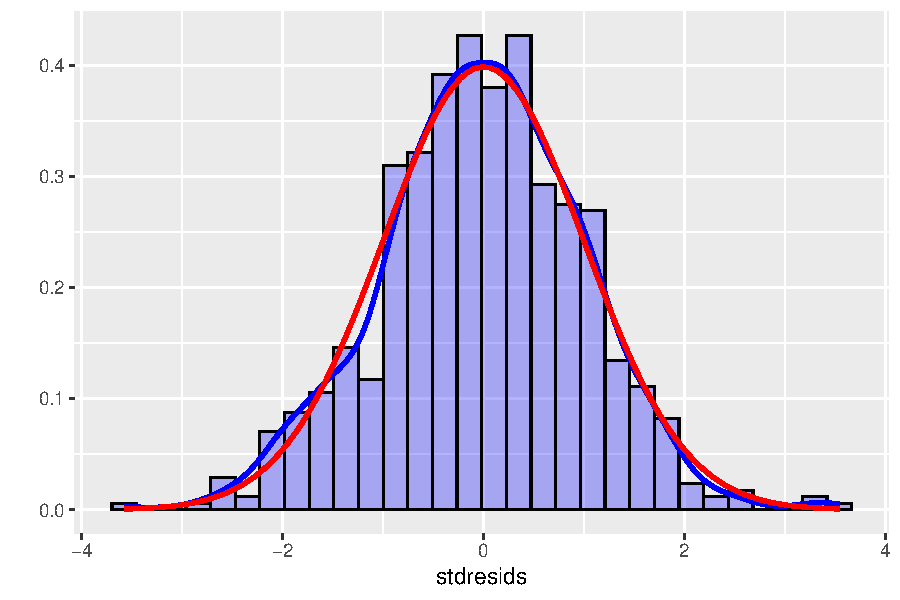
\includegraphics[width=0.65\linewidth,height=\textheight,keepaspectratio]{chapters/../figures/fig-hist-residuals-1.pdf}

}

\caption{\label{fig-hist-residuals}Histograma de residuales
estandarizados con curva de densidad estimada y distribución normal
teórica}

\end{figure}%

Según Chambers y Skinner (\citeproc{ref-ChambersSkinner2003}{2003}), la
homocedasticidad de los errores (varianza constante) constituye uno de
los supuestos centrales en los modelos de regresión. Su incumplimiento
afecta la eficiencia de los estimadores y las varianzas basadas
exclusivamente en el modelo; las varianzas robustas ajustadas al diseño
ofrecen protección adicional, aunque no corrigen una especificación
incorrecta de la media. Dado que los residuos representan las
discrepancias entre los valores observados y los valores ajustados por
el modelo, su análisis en función de los valores predichos o de las
covariables constituye una herramienta diagnóstica fundamental. Bajo un
modelo adecuadamente especificado, se espera que los residuos se
distribuyan de forma aleatoria alrededor de cero, sin patrones
estructurados; en cambio, la aparición de formas sistemáticas (como
estructuras en embudo o curvaturas) sugiere la presencia de
heterocedasticidad (varianza no constante) o posibles relaciones
funcionales no captadas por la especificación del modelo.

Para evaluar este supuesto, se analizan gráficamente los residuos en
función de los valores estimados \(\hat{\mu}_{k}\) o de covariables
específicas del modelo. La aparición de patrones sistemáticos en estos
gráficos constituye evidencia de heterocedasticidad o de posibles
problemas de especificación funcional. El siguiente código computacional
construye gráficos de residuos frente a las covariables del modelo y los
combina con \texttt{patchwork} en la
figura~\ref{fig-residuals-covariates}.

\begin{Shaded}
\begin{Highlighting}[]
\FunctionTok{library}\NormalTok{(patchwork)}

\NormalTok{g1 }\OtherTok{\textless{}{-}} \FunctionTok{ggplot}\NormalTok{(}
  \AttributeTok{data =}\NormalTok{ survey\_design}\SpecialCharTok{$}\NormalTok{variables,}
  \FunctionTok{aes}\NormalTok{(}\AttributeTok{x =} \FunctionTok{log}\NormalTok{(Income), }\AttributeTok{y =}\NormalTok{ stdresids)}
\NormalTok{) }\SpecialCharTok{+}
  \FunctionTok{geom\_point}\NormalTok{() }\SpecialCharTok{+}
  \FunctionTok{geom\_hline}\NormalTok{(}\AttributeTok{yintercept =} \DecValTok{0}\NormalTok{)}

\NormalTok{g2 }\OtherTok{\textless{}{-}} \FunctionTok{ggplot}\NormalTok{(}
  \AttributeTok{data =}\NormalTok{ survey\_design}\SpecialCharTok{$}\NormalTok{variables,}
  \FunctionTok{aes}\NormalTok{(}\AttributeTok{x =}\NormalTok{ Zone, }\AttributeTok{y =}\NormalTok{ stdresids)}
\NormalTok{) }\SpecialCharTok{+}
  \FunctionTok{geom\_point}\NormalTok{() }\SpecialCharTok{+}
  \FunctionTok{geom\_hline}\NormalTok{(}\AttributeTok{yintercept =} \DecValTok{0}\NormalTok{)}

\NormalTok{g3 }\OtherTok{\textless{}{-}} \FunctionTok{ggplot}\NormalTok{(}
  \AttributeTok{data =}\NormalTok{ survey\_design}\SpecialCharTok{$}\NormalTok{variables,}
  \FunctionTok{aes}\NormalTok{(}\AttributeTok{x =}\NormalTok{ Sex, }\AttributeTok{y =}\NormalTok{ stdresids)}
\NormalTok{) }\SpecialCharTok{+}
  \FunctionTok{geom\_point}\NormalTok{() }\SpecialCharTok{+}
  \FunctionTok{geom\_hline}\NormalTok{(}\AttributeTok{yintercept =} \DecValTok{0}\NormalTok{)}

\NormalTok{g4 }\OtherTok{\textless{}{-}} \FunctionTok{ggplot}\NormalTok{(}
  \AttributeTok{data =}\NormalTok{ survey\_design}\SpecialCharTok{$}\NormalTok{variables,}
  \FunctionTok{aes}\NormalTok{(}\AttributeTok{x =}\NormalTok{ Age, }\AttributeTok{y =}\NormalTok{ stdresids)}
\NormalTok{) }\SpecialCharTok{+}
  \FunctionTok{geom\_point}\NormalTok{() }\SpecialCharTok{+}
  \FunctionTok{geom\_hline}\NormalTok{(}\AttributeTok{yintercept =} \DecValTok{0}\NormalTok{)}

\NormalTok{g5 }\OtherTok{\textless{}{-}} \FunctionTok{ggplot}\NormalTok{(}
  \AttributeTok{data =}\NormalTok{ survey\_design}\SpecialCharTok{$}\NormalTok{variables,}
  \FunctionTok{aes}\NormalTok{(}\AttributeTok{x =}\NormalTok{ Region, }\AttributeTok{y =}\NormalTok{ stdresids)}
\NormalTok{) }\SpecialCharTok{+}
  \FunctionTok{geom\_point}\NormalTok{() }\SpecialCharTok{+}
  \FunctionTok{geom\_hline}\NormalTok{(}\AttributeTok{yintercept =} \DecValTok{0}\NormalTok{)}

\NormalTok{(g1 }\SpecialCharTok{|}\NormalTok{ g4) }\SpecialCharTok{/}\NormalTok{ (g2 }\SpecialCharTok{|}\NormalTok{ g3) }\SpecialCharTok{/}\NormalTok{ g5}
\end{Highlighting}
\end{Shaded}

\begin{figure}[H]

\centering{

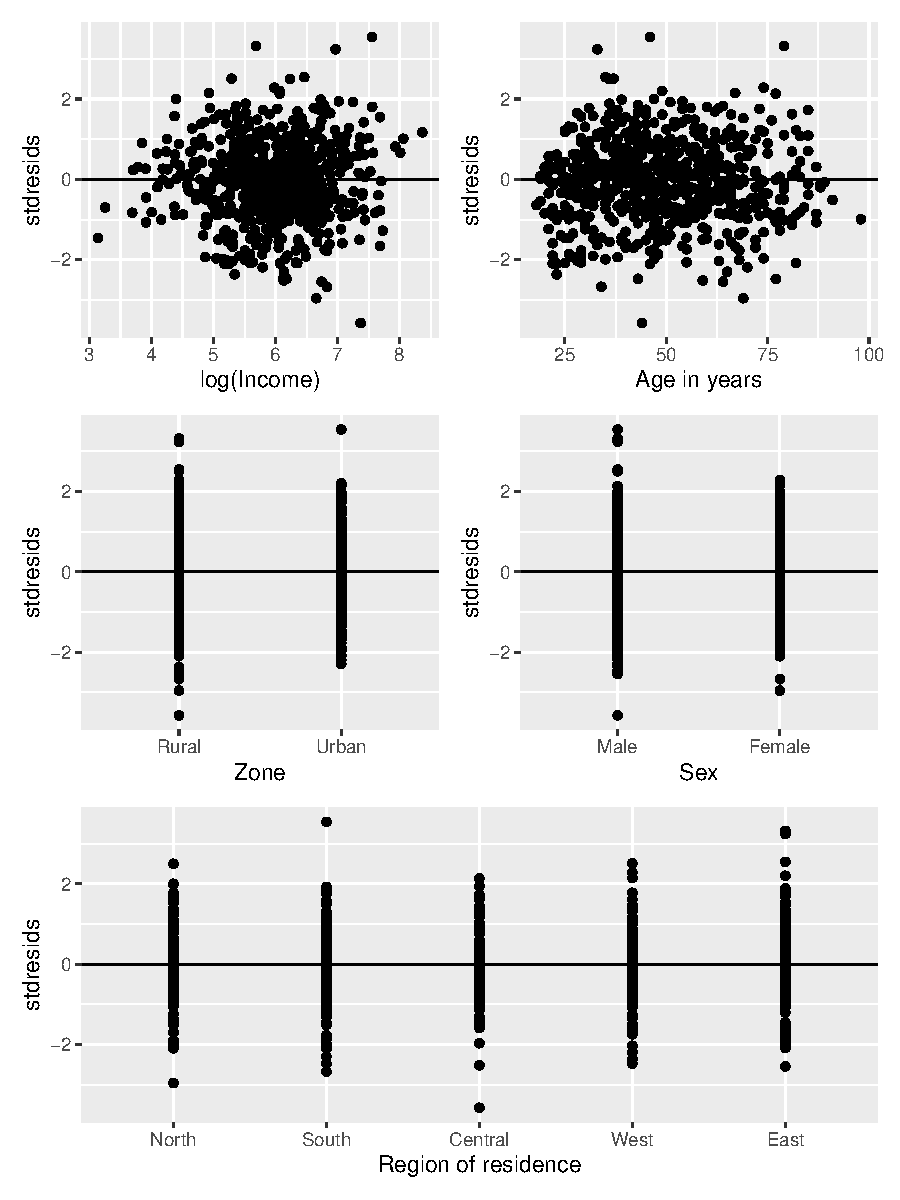
\includegraphics[width=0.8\linewidth,height=\textheight,keepaspectratio]{chapters/../figures/fig-residuals-covariates-1.pdf}

}

\caption{\label{fig-residuals-covariates}Gráficos de residuales
estandarizados frente a cada covariable del modelo}

\end{figure}%

La figura~\ref{fig-residuals-covariates} presenta los gráficos de
dispersión de los residuos estandarizados frente a las covariables del
modelo. En conjunto, estos resultados permiten examinar posibles
limitaciones en la especificación funcional. En particular, los gráficos
frente a \texttt{log(Income)} y \texttt{Age} permiten buscar curvaturas
o cambios en la dispersión que no estén captados por el modelo. Por su
parte, en los gráficos asociados a \texttt{Zone}, \texttt{Sex} y
\texttt{Region} se compara la dispersión de los residuos entre
categorías, lo que contribuye a evaluar diferencias en la variabilidad
condicional o en el ajuste de la media entre grupos.

\subsection{Observaciones influyentes}\label{observaciones-influyentes}

En el análisis diagnóstico, la identificación de observaciones
influyentes es una técnica de especial importancia. Estas son unidades
muestrales cuyo impacto sobre el ajuste del modelo resulta
desproporcionado respecto al resto de la muestra. Conviene subrayar que
una observación influyente no necesariamente corresponde a un valor
atípico: mientras un atípico puede estar alejado del patrón general de
los datos sin afectar sustancialmente el ajuste, una observación
influyente puede alterar de manera significativa las estimaciones de los
parámetros, incluso si no luce inusual.

Según Heeringa et~al. (\citeproc{ref-HeeringaWestBerglund2017}{2017,
213}), la distancia de Cook mide el impacto que tendría la eliminación
de la observación \(k\) sobre el ajuste global del modelo, al combinar
simultáneamente la magnitud del residuo, la varianza estimada del modelo
y su apalancamiento (\emph{leverage}). En el contexto de encuestas con
diseños muestrales complejos, la distancia de Cook suele denotarse como
\(c_k\) y su expresión incorpora explícitamente los pesos muestrales.
Para evaluar la magnitud de este estadístico, se utiliza una
aproximación basada en su comparación con una distribución \(F\),
mediante la expresión:

\[
\frac{(df-p+1)\,c_{k}}{df} \sim F_{(p,\,df-p)},
\]

Donde \(p\) denota los parámetros del modelo y \(df\) representa los
grados de libertad asociados al diseño muestral. En la práctica, una
observación puede considerarse influyente si su distancia de Cook supera
valores de referencia aproximados entre 2 y 3. El siguiente código
computacional genera la figura~\ref{fig-cook}.

\begin{Shaded}
\begin{Highlighting}[]
\NormalTok{cook\_values }\OtherTok{\textless{}{-}} \FunctionTok{svyCooksD}\NormalTok{(fit\_svy, }\AttributeTok{doplot =} \ConstantTok{TRUE}\NormalTok{)}
\end{Highlighting}
\end{Shaded}

\begin{figure}[H]

\centering{

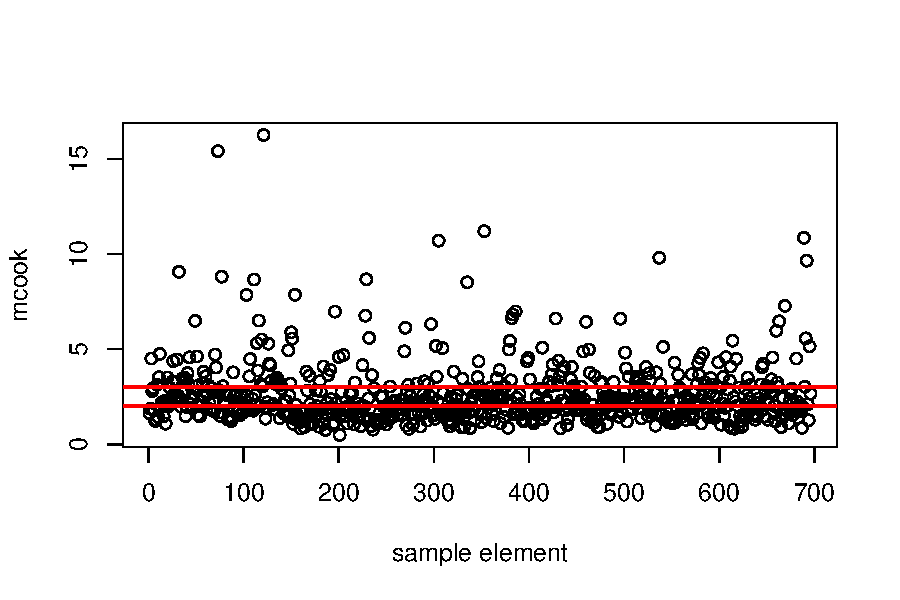
\includegraphics[width=0.65\linewidth,height=\textheight,keepaspectratio]{chapters/../figures/fig-cook-1.pdf}

}

\caption{\label{fig-cook}Distancia de Cook para cada observación de la
muestra}

\end{figure}%

En \texttt{R}, se evalúa la presencia de observaciones influyentes
mediante la distancia de Cook, estimada con la función
\texttt{svyCooksD} del paquete \texttt{svydiags}. Los resultados
obtenidos se presentan en la figura~\ref{fig-cook}, en donde se observa
que 177 de los 696 hogares superan el umbral de referencia de 3 y la
distancia máxima es 16,27. Bajo este criterio diagnóstico, estas
observaciones requieren una revisión más detallada de su influencia
sobre el ajuste, sin que ello implique eliminarlas automáticamente.

Otro estadístico que mide el grado de influencia de una observación es
el DFBETAS, denotado como \(D_f\text{Beta}_{(k)j}\), que mide el cambio
que experimenta el coeficiente de regresión \(\hat{\beta}_{j}\) cuando
la observación \(k\) es eliminada del proceso de estimación. En
consecuencia, esta medida evalúa la influencia individual de cada
observación sobre los parámetros del modelo, identificando aquellas
unidades cuya presencia altera de manera importante las estimaciones
obtenidas. Valores elevados de \(D_f\text{Beta}_{(k)j}\) indican que la
observación ejerce una influencia considerable sobre el coeficiente
correspondiente, lo que puede afectar la estabilidad e interpretación
del modelo.

Como criterio práctico de diagnóstico, Li y Valliant
(\citeproc{ref-Li_Valliant_2015}{2015}) señalan que una observación
suele considerarse influyente sobre el coeficiente \(\hat{\beta}_{j}\)
cuando

\[
\left|D_f\text{Beta}_{(k)j}\right|
\geq
\frac{z}{\sqrt{n_I\times DEFF}},
\]

Donde \(z\) toma comúnmente valores de 2 o 3, \(n_I\) representa el
número de UPMs seleccionadas en la muestra de la primera etapa y
\(DEFF\) corresponde al efecto de diseño asociado a la variable
respuesta. A continuación, se evalúa la influencia de las observaciones
sobre los coeficientes del modelo de ejemplo mediante la función
\texttt{svydfbetas}. Los resultados de las primeras diez observaciones
se presentan en la tabla~\ref{tbl-dfbetas-primeros}, junto con el
identificador del hogar (\texttt{HHID}). Las columnas Beta 0 a Beta 8
siguen el orden de los coeficientes del modelo: intercepto, logaritmo
del ingreso, edad, sexo femenino, zona urbana y regiones Sur, Centro,
Occidente y Oriente.

\begin{Shaded}
\begin{Highlighting}[]
\NormalTok{d\_dfbetas }\OtherTok{\textless{}{-}} \FunctionTok{data.frame}\NormalTok{(}\FunctionTok{t}\NormalTok{(}\FunctionTok{svydfbetas}\NormalTok{(fit\_svy)}\SpecialCharTok{$}\NormalTok{Dfbetas))}
\FunctionTok{colnames}\NormalTok{(d\_dfbetas) }\OtherTok{\textless{}{-}} \FunctionTok{paste0}\NormalTok{(}\StringTok{"Beta\_"}\NormalTok{, }\DecValTok{0}\SpecialCharTok{:}\NormalTok{(}\FunctionTok{length}\NormalTok{(}\FunctionTok{coef}\NormalTok{(fit\_svy)) }\SpecialCharTok{{-}} \DecValTok{1}\NormalTok{))}
\NormalTok{dfbetas\_first\_ten\_table }\OtherTok{\textless{}{-}}\NormalTok{ d\_dfbetas }\SpecialCharTok{\%\textgreater{}\%}
  \FunctionTok{slice}\NormalTok{(}\DecValTok{1}\SpecialCharTok{:}\DecValTok{10}\NormalTok{L) }\SpecialCharTok{\%\textgreater{}\%}
  \FunctionTok{mutate}\NormalTok{(}\AttributeTok{HHID =}\NormalTok{ survey\_data}\SpecialCharTok{$}\NormalTok{HHID[}\DecValTok{1}\SpecialCharTok{:}\DecValTok{10}\NormalTok{], }\AttributeTok{.before =} \DecValTok{1}\NormalTok{)}

\NormalTok{dfbetas\_first\_ten\_table}
\end{Highlighting}
\end{Shaded}

{

\begin{longtable}[]{@{}
  >{\raggedright\arraybackslash}p{(\linewidth - 18\tabcolsep) * \real{0.1529}}
  >{\raggedleft\arraybackslash}p{(\linewidth - 18\tabcolsep) * \real{0.0941}}
  >{\raggedleft\arraybackslash}p{(\linewidth - 18\tabcolsep) * \real{0.0941}}
  >{\raggedleft\arraybackslash}p{(\linewidth - 18\tabcolsep) * \real{0.0941}}
  >{\raggedleft\arraybackslash}p{(\linewidth - 18\tabcolsep) * \real{0.0941}}
  >{\raggedleft\arraybackslash}p{(\linewidth - 18\tabcolsep) * \real{0.0941}}
  >{\raggedleft\arraybackslash}p{(\linewidth - 18\tabcolsep) * \real{0.0941}}
  >{\raggedleft\arraybackslash}p{(\linewidth - 18\tabcolsep) * \real{0.0941}}
  >{\raggedleft\arraybackslash}p{(\linewidth - 18\tabcolsep) * \real{0.0941}}
  >{\raggedleft\arraybackslash}p{(\linewidth - 18\tabcolsep) * \real{0.0941}}@{}}

\caption{\label{tbl-dfbetas-primeros}Valores DfBetas para las primeras
diez observaciones de la muestra, con identificador del hogar}

\tabularnewline

\toprule\noalign{}
\begin{minipage}[b]{\linewidth}\raggedright
ID del hogar
\end{minipage} & \begin{minipage}[b]{\linewidth}\raggedleft
Beta 0
\end{minipage} & \begin{minipage}[b]{\linewidth}\raggedleft
Beta 1
\end{minipage} & \begin{minipage}[b]{\linewidth}\raggedleft
Beta 2
\end{minipage} & \begin{minipage}[b]{\linewidth}\raggedleft
Beta 3
\end{minipage} & \begin{minipage}[b]{\linewidth}\raggedleft
Beta 4
\end{minipage} & \begin{minipage}[b]{\linewidth}\raggedleft
Beta 5
\end{minipage} & \begin{minipage}[b]{\linewidth}\raggedleft
Beta 6
\end{minipage} & \begin{minipage}[b]{\linewidth}\raggedleft
Beta 7
\end{minipage} & \begin{minipage}[b]{\linewidth}\raggedleft
Beta 8
\end{minipage} \\
\midrule\noalign{}
\endhead
\bottomrule\noalign{}
\endlastfoot
idHH00031 & -0.0009 & 0.0044 & 0.0267 & -0.0114 & -0.0147 & -0.0255 &
-0.0251 & -0.0300 & -0.0253 \\
idHH00041 & -0.0055 & 0.0068 & 0.0037 & 0.0069 & -0.0057 & -0.0064 &
-0.0071 & -0.0081 & -0.0073 \\
idHH20680 & -0.0307 & 0.0244 & -0.0149 & 0.0161 & 0.0083 & 0.0266 &
0.0238 & 0.0309 & 0.0231 \\
idHH00064 & -0.0227 & 0.0229 & -0.0559 & 0.0240 & 0.0145 & 0.0355 &
0.0337 & 0.0434 & 0.0320 \\
idHH20700 & 0.0043 & 0.0007 & -0.0038 & -0.0030 & -0.0051 & -0.0102 &
-0.0094 & -0.0111 & -0.0100 \\
idHH20705 & -0.0053 & 0.0067 & 0.0042 & -0.0013 & -0.0046 & -0.0059 &
-0.0061 & -0.0067 & -0.0065 \\
idHH20845 & -0.0020 & 0.0008 & 0.0013 & 0.0014 & -0.0025 & 0.0036 &
0.0037 & 0.0037 & 0.0033 \\
idHH20854 & 0.0162 & -0.0114 & 0.0008 & -0.0099 & 0.0147 & -0.0198 &
-0.0203 & -0.0210 & -0.0175 \\
idHH20858 & -0.0017 & -0.0050 & 0.0054 & 0.0060 & -0.0114 & 0.0202 &
0.0216 & 0.0208 & 0.0197 \\
idHH20859 & 0.0188 & -0.0202 & -0.0180 & -0.0237 & -0.0098 & 0.0282 &
0.0342 & 0.0335 & 0.0303 \\

\end{longtable}

}

A partir de los valores DFBETA de cada observación y coeficiente del
modelo, el siguiente código computacional calcula el correspondiente
umbral de influencia a partir de los resultados generados por la función
\texttt{svydfbetas}. Con base en este criterio, se construye una
variable dicotómica que permite clasificar las observaciones según su
nivel de influencia sobre las estimaciones del modelo. Los resultados de
esta clasificación se presentan en la
tabla~\ref{tbl-dfbetas-influyentes}.

\begin{Shaded}
\begin{Highlighting}[]
\NormalTok{d\_dfbetas}\SpecialCharTok{$}\NormalTok{id }\OtherTok{\textless{}{-}} \DecValTok{1}\SpecialCharTok{:}\FunctionTok{nrow}\NormalTok{(d\_dfbetas)}
\NormalTok{d\_dfbetas }\OtherTok{\textless{}{-}}\NormalTok{ reshape2}\SpecialCharTok{::}\FunctionTok{melt}\NormalTok{(d\_dfbetas, }\AttributeTok{id.vars =} \StringTok{"id"}\NormalTok{)}
\NormalTok{cutoff }\OtherTok{\textless{}{-}} \FunctionTok{svydfbetas}\NormalTok{(fit\_svy)}\SpecialCharTok{$}\NormalTok{cutoff}
\NormalTok{d\_dfbetas }\OtherTok{\textless{}{-}}\NormalTok{ d\_dfbetas }\SpecialCharTok{\%\textgreater{}\%}
  \FunctionTok{mutate}\NormalTok{(}
    \AttributeTok{criterion =} \FunctionTok{ifelse}\NormalTok{(}\FunctionTok{abs}\NormalTok{(value) }\SpecialCharTok{\textgreater{}}\NormalTok{ cutoff, }\StringTok{"Yes"}\NormalTok{, }\StringTok{"No"}\NormalTok{ )}
\NormalTok{  )}

\NormalTok{label\_text }\OtherTok{\textless{}{-}}\NormalTok{ d\_dfbetas }\SpecialCharTok{\%\textgreater{}\%}
  \FunctionTok{filter}\NormalTok{(criterion }\SpecialCharTok{==} \StringTok{"Yes"}\NormalTok{) }\SpecialCharTok{\%\textgreater{}\%}
  \FunctionTok{arrange}\NormalTok{(}\FunctionTok{desc}\NormalTok{(}\FunctionTok{abs}\NormalTok{(value))) }\SpecialCharTok{\%\textgreater{}\%}
  \FunctionTok{slice}\NormalTok{(}\DecValTok{1}\SpecialCharTok{:}\DecValTok{10}\NormalTok{L)}

\NormalTok{influential\_dfbetas\_table }\OtherTok{\textless{}{-}}\NormalTok{ label\_text }\SpecialCharTok{\%\textgreater{}\%}
  \FunctionTok{mutate}\NormalTok{(}\AttributeTok{HHID =}\NormalTok{ survey\_data}\SpecialCharTok{$}\NormalTok{HHID[id]) }\SpecialCharTok{\%\textgreater{}\%}
\NormalTok{  dplyr}\SpecialCharTok{::}\FunctionTok{select}\NormalTok{(}\SpecialCharTok{{-}}\NormalTok{id) }\SpecialCharTok{\%\textgreater{}\%}
  \FunctionTok{relocate}\NormalTok{(HHID)}

\NormalTok{influential\_dfbetas\_table}
\end{Highlighting}
\end{Shaded}

{

\begin{longtable}[]{@{}llrl@{}}

\caption{\label{tbl-dfbetas-influyentes}Las diez observaciones más
influyentes según el criterio DfBetas, con identificador del hogar}

\tabularnewline

\toprule\noalign{}
ID del hogar & Parámetro & Valor & Criterio \\
\midrule\noalign{}
\endhead
\bottomrule\noalign{}
\endlastfoot
idHH20102 & Beta\_3 & -0.4100 & Yes \\
idHH18379 & Beta\_8 & -0.3663 & Yes \\
idHH39024 & Beta\_8 & -0.3663 & Yes \\
idHH20102 & Beta\_2 & 0.3482 & Yes \\
idHH20102 & Beta\_8 & -0.3244 & Yes \\
idHH02136 & Beta\_0 & 0.2910 & Yes \\
idHH20102 & Beta\_4 & 0.2684 & Yes \\
idHH35243 & Beta\_7 & 0.2684 & Yes \\
idHH18379 & Beta\_4 & 0.2682 & Yes \\
idHH39024 & Beta\_4 & 0.2682 & Yes \\

\end{longtable}

}

Los resultados muestran que 106 combinaciones de observación y
coeficiente superan el umbral establecido por el criterio DFBETAS, lo
que indica que dichas unidades ejercen una influencia importante sobre
la estimación de algunos coeficientes del modelo, sugiriendo la
presencia de unidades con alto impacto sobre la estabilidad del ajuste.
La figura~\ref{fig-dfbetas}, obtenida con el siguiente código
computacional, muestra la representación gráfica de los valores de
\(D_f\text{Beta}\) junto con el umbral de referencia utilizado para
identificar observaciones influyentes. En la figura, los puntos
resaltados en rojo corresponden a las observaciones que exceden dicho
umbral y que, por tanto, requieren una revisión más detallada dentro del
proceso de diagnóstico del modelo.

\begin{Shaded}
\begin{Highlighting}[]
\FunctionTok{ggplot}\NormalTok{(d\_dfbetas, }\FunctionTok{aes}\NormalTok{(}\AttributeTok{y =} \FunctionTok{abs}\NormalTok{(value), }\AttributeTok{x =}\NormalTok{ id)) }\SpecialCharTok{+}
  \FunctionTok{geom\_point}\NormalTok{(}\FunctionTok{aes}\NormalTok{(}\AttributeTok{col =}\NormalTok{ criterion)) }\SpecialCharTok{+}
  \FunctionTok{geom\_text}\NormalTok{(}
    \AttributeTok{data =}\NormalTok{ label\_text,}
    \AttributeTok{angle =} \DecValTok{45}\NormalTok{,}
    \AttributeTok{vjust =} \SpecialCharTok{{-}}\DecValTok{1}\NormalTok{,}
    \FunctionTok{aes}\NormalTok{(}\AttributeTok{label =}\NormalTok{ id)}
\NormalTok{  ) }\SpecialCharTok{+}
  \FunctionTok{geom\_hline}\NormalTok{(}\FunctionTok{aes}\NormalTok{(}\AttributeTok{yintercept =}\NormalTok{ cutoff)) }\SpecialCharTok{+}
  \FunctionTok{facet\_wrap}\NormalTok{(. }\SpecialCharTok{\textasciitilde{}}\NormalTok{ variable, }\AttributeTok{nrow =} \DecValTok{3}\NormalTok{) }\SpecialCharTok{+}
  \FunctionTok{scale\_color\_manual}\NormalTok{(}
    \AttributeTok{values =} \FunctionTok{c}\NormalTok{(}\StringTok{"Yes"} \OtherTok{=} \StringTok{"red"}\NormalTok{, }\StringTok{"No"} \OtherTok{=} \StringTok{"black"}\NormalTok{)}
\NormalTok{  )}
\end{Highlighting}
\end{Shaded}

\begin{figure}[H]

\centering{

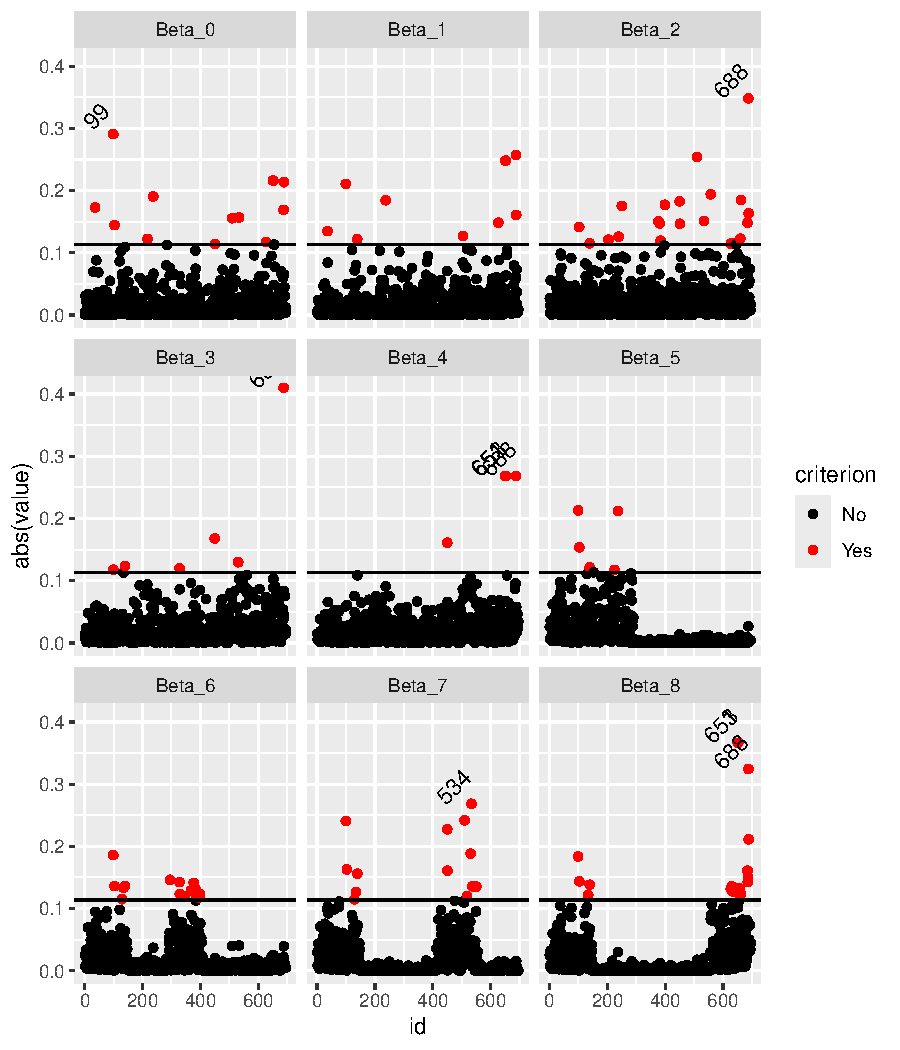
\includegraphics[width=0.8\linewidth,height=\textheight,keepaspectratio]{chapters/../figures/fig-dfbetas-1.pdf}

}

\caption{\label{fig-dfbetas}Valores DfBetas por parámetro: observaciones
influyentes señaladas en rojo}

\end{figure}%

Por último, el estadístico DFFITS, denotado por
\(D_f\text{Fits}_{(k)}\), mide la influencia que ejerce la observación
\(k\) sobre los valores ajustados del modelo. En particular, este
estadístico evalúa cuánto cambian las predicciones del modelo cuando una
observación es eliminada del proceso de estimación. En consecuencia,
valores elevados de \(D_f\text{Fits}_{(k)}\) indican observaciones con
capacidad de alterar de manera importante el ajuste global del modelo y,
por tanto, potencialmente influyentes en el proceso de inferencia. Una
observación se considera influyente si:

\[
|D_f\text{Fits}_{(k)}| \geq z\sqrt{\frac{p}{n\times DEFF}}
\]

Donde \(z\) toma comúnmente valores de 2 o 3, mientras que \(n\)
representa el tamaño muestral total de elementos incluidos en la
encuesta y \(DEFF\) es el efecto de diseño asociado a la variable
respuesta. En \texttt{R}, el cálculo de este estadístico puede
realizarse mediante la función \texttt{svydffits} del paquete
\texttt{svydiags}, la cual obtiene las medidas de influencia
considerando explícitamente la estructura del diseño muestral. El
siguiente código computacional genera la figura~\ref{fig-dffits}.

\begin{Shaded}
\begin{Highlighting}[]
\NormalTok{d\_dffits }\OtherTok{\textless{}{-}} \FunctionTok{data.frame}\NormalTok{(}
  \AttributeTok{dffits =} \FunctionTok{svydffits}\NormalTok{(fit\_svy)}\SpecialCharTok{$}\NormalTok{Dffits,}
  \AttributeTok{id =} \DecValTok{1}\SpecialCharTok{:}\FunctionTok{length}\NormalTok{(}\FunctionTok{svydffits}\NormalTok{(fit\_svy)}\SpecialCharTok{$}\NormalTok{Dffits)}
\NormalTok{)}
\NormalTok{cutoff }\OtherTok{\textless{}{-}} \FunctionTok{svydffits}\NormalTok{(fit\_svy)}\SpecialCharTok{$}\NormalTok{cutoff}
\NormalTok{d\_dffits }\OtherTok{\textless{}{-}}\NormalTok{ d\_dffits }\SpecialCharTok{\%\textgreater{}\%}
  \FunctionTok{mutate}\NormalTok{(}
    \AttributeTok{cutoff\_criterion =} \FunctionTok{ifelse}\NormalTok{(}\FunctionTok{abs}\NormalTok{(dffits) }\SpecialCharTok{\textgreater{}}\NormalTok{ cutoff, }\StringTok{"Yes"}\NormalTok{, }\StringTok{"No"}\NormalTok{)}
\NormalTok{  )}

\FunctionTok{ggplot}\NormalTok{(d\_dffits, }\FunctionTok{aes}\NormalTok{(}\AttributeTok{y =} \FunctionTok{abs}\NormalTok{(dffits), }\AttributeTok{x =}\NormalTok{ id)) }\SpecialCharTok{+}
  \FunctionTok{geom\_point}\NormalTok{(}\FunctionTok{aes}\NormalTok{(}\AttributeTok{col =}\NormalTok{ cutoff\_criterion)) }\SpecialCharTok{+}
  \FunctionTok{geom\_hline}\NormalTok{(}\AttributeTok{yintercept =}\NormalTok{ cutoff) }\SpecialCharTok{+}
  \FunctionTok{scale\_color\_manual}\NormalTok{(}
    \AttributeTok{values =} \FunctionTok{c}\NormalTok{(}\StringTok{"Yes"} \OtherTok{=} \StringTok{"red"}\NormalTok{, }\StringTok{"No"} \OtherTok{=} \StringTok{"black"}\NormalTok{)}
\NormalTok{  )}
\end{Highlighting}
\end{Shaded}

\begin{figure}[H]

\centering{

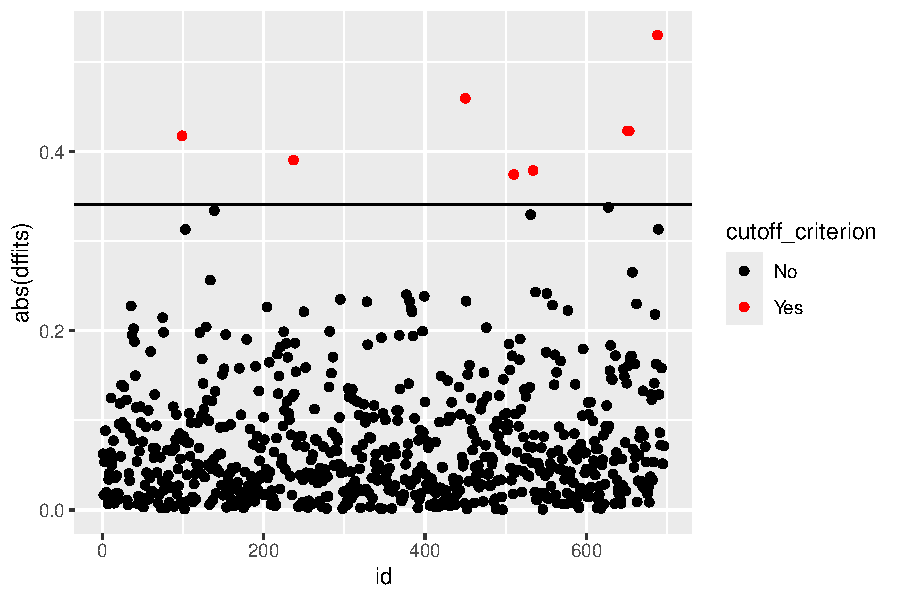
\includegraphics[width=0.65\linewidth,height=\textheight,keepaspectratio]{chapters/../figures/fig-dffits-1.pdf}

}

\caption{\label{fig-dffits}Valores DfFits: observaciones influyentes
sobre el ajuste global señaladas en rojo}

\end{figure}%

Los resultados gráficos correspondientes se presentan en la
figura~\ref{fig-dffits}, en donde se identifican 8 observaciones que
superan el umbral de influencia (señaladas en rojo).

\section{Inferencia sobre los parámetros del
modelo}\label{inferencia-sobre-los-parametros-del-modelo}

Una vez evaluado el ajuste del modelo y examinados los supuestos
asociados a los errores, el siguiente paso consiste en determinar la
significación estadística de los parámetros estimados. Este análisis
permite establecer si las covariables incluidas en el modelo aportan
información relevante para explicar la variabilidad de la variable
respuesta. De acuerdo con Chambers y Skinner
(\citeproc{ref-ChambersSkinner2003}{2003}) y Heeringa et~al.
(\citeproc{ref-HeeringaWestBerglund2017}{2017}), en modelos ajustados
con datos provenientes de encuestas complejas, las pruebas de hipótesis
sobre los coeficientes de regresión se construyen utilizando estimadores
de varianza consistentes con el diseño muestral. Para evaluar el efecto
de una covariable asociada al parámetro \(\beta_j\), se considera
usualmente el contraste

\[
H_0:\beta_j=0
\qquad \text{frente a} \qquad
H_1:\beta_j\neq 0.
\]

El estadístico de prueba correspondiente se define como

\begin{equation}\protect\phantomsection\label{eq-prueba-coeficiente-regresion}{
t_j=
\frac{\hat{\beta}_{j}-\beta_{j}}
{\sqrt{\widehat{Var}(\hat{\beta}_{j})}}
}\end{equation}

el cual, bajo la hipótesis nula sigue aproximadamente una distribución
\(t\) de Student con \(df\) grados de libertad asociados al diseño
muestral (usualmente definidos como el número de unidades primarias de
muestreo menos el número de estratos). La decisión inferencial se basa
en comparar el valor absoluto del estadístico \(t_j\) con el valor
crítico de la distribución de referencia. Cuando el valor observado del
estadístico resulta suficientemente grande en magnitud, se rechaza la
hipótesis nula y se concluye que la covariable correspondiente presenta
una asociación estadísticamente significativa con la variable respuesta.
Por tanto, el valor-\emph{p} cuantifica qué tan compatible es el
resultado observado con la hipótesis nula \(H_0:\beta_j=0\). En una
prueba bilateral, corresponde a la probabilidad, suponiendo verdadera
dicha hipótesis, de obtener un estadístico de prueba tan extremo o más
extremo que el observado, en cualquiera de las dos direcciones. A partir
del estadístico \(t_j\) de la expresión (5.4), se calcula como:

\[
\text{valor-}p
=
2\,\Pr\!\left(T\geq |t_j|\right).
\]

En donde \(T\) sigue una distribución \(t\) de Student con \(df\) grados
de libertad bajo \(H_0\). Un valor-\emph{p} pequeño indica mayor
incompatibilidad con la hipótesis nula; si es menor que \(\alpha\), se
rechaza \(H_0\) al nivel de significación \(\alpha\). Las mismas
propiedades distribucionales permiten construir intervalos de confianza
para los coeficientes de regresión. Así, un intervalo de confianza al
nivel \((1-\alpha)\times100\%\) para el parámetro \(\beta_j\) está dado
por

\begin{equation}\protect\phantomsection\label{eq-intervalo-coeficiente-regresion}{
\hat{\beta}_{j}
\pm
t_{1-\frac{\alpha}{2},\,df}
\sqrt{\widehat{Var}(\hat{\beta}_{j})},
}\end{equation}

donde \(t_{1-\frac{\alpha}{2},\,df}\) representa el cuantil de orden
\(1-\alpha/2\) de la distribución \(t\) de Student con \(df\) grados de
libertad.

Para implementar estos procedimientos en \texttt{R}, se utilizan las
funciones \texttt{summary.svyglm} y \texttt{confint.svyglm}, las cuales
permiten obtener, respectivamente, las pruebas de significación basadas
en el estadístico \(t\) y los intervalos de confianza de los
coeficientes estimados bajo el diseño muestral complejo. Los resultados
correspondientes se presentan en la tabla~\ref{tbl-inferencia-modelo}.
El siguiente código computacional extrae las estimaciones y los
resultados de las pruebas de los coeficientes del modelo.

\begin{Shaded}
\begin{Highlighting}[]
\NormalTok{summary\_table }\OtherTok{\textless{}{-}} \FunctionTok{summary}\NormalTok{(fit\_svy)}\SpecialCharTok{$}\NormalTok{coefficients }\SpecialCharTok{\%\textgreater{}\%}
  \FunctionTok{as.data.frame}\NormalTok{() }\SpecialCharTok{\%\textgreater{}\%}
\NormalTok{  tibble}\SpecialCharTok{::}\FunctionTok{rownames\_to\_column}\NormalTok{(}\StringTok{"Parameter"}\NormalTok{)}

\NormalTok{confidence\_table }\OtherTok{\textless{}{-}} \FunctionTok{confint}\NormalTok{(fit\_svy) }\SpecialCharTok{\%\textgreater{}\%}
  \FunctionTok{as.data.frame}\NormalTok{() }\SpecialCharTok{\%\textgreater{}\%}
\NormalTok{  tibble}\SpecialCharTok{::}\FunctionTok{rownames\_to\_column}\NormalTok{(}\StringTok{"Parameter"}\NormalTok{)}

\NormalTok{summary\_table }\OtherTok{\textless{}{-}}\NormalTok{ dplyr}\SpecialCharTok{::}\FunctionTok{left\_join}\NormalTok{(}
\NormalTok{  summary\_table,}
\NormalTok{  confidence\_table,}
  \AttributeTok{by =} \StringTok{"Parameter"}
\NormalTok{)}

\NormalTok{summary\_table}
\end{Highlighting}
\end{Shaded}

{

\begin{longtable}[]{@{}
  >{\raggedright\arraybackslash}p{(\linewidth - 12\tabcolsep) * \real{0.2059}}
  >{\raggedleft\arraybackslash}p{(\linewidth - 12\tabcolsep) * \real{0.1618}}
  >{\raggedleft\arraybackslash}p{(\linewidth - 12\tabcolsep) * \real{0.1029}}
  >{\raggedleft\arraybackslash}p{(\linewidth - 12\tabcolsep) * \real{0.1765}}
  >{\raggedleft\arraybackslash}p{(\linewidth - 12\tabcolsep) * \real{0.1176}}
  >{\raggedleft\arraybackslash}p{(\linewidth - 12\tabcolsep) * \real{0.1176}}
  >{\raggedleft\arraybackslash}p{(\linewidth - 12\tabcolsep) * \real{0.1176}}@{}}

\caption{\label{tbl-inferencia-modelo}Pruebas t e intervalos de
confianza al 95\% para los parámetros del modelo}

\tabularnewline

\toprule\noalign{}
\begin{minipage}[b]{\linewidth}\raggedright
Parámetro
\end{minipage} & \begin{minipage}[b]{\linewidth}\raggedleft
Estimación
\end{minipage} & \begin{minipage}[b]{\linewidth}\raggedleft
EE
\end{minipage} & \begin{minipage}[b]{\linewidth}\raggedleft
Estadístico
\end{minipage} & \begin{minipage}[b]{\linewidth}\raggedleft
Valor p
\end{minipage} & \begin{minipage}[b]{\linewidth}\raggedleft
LI 95 \%
\end{minipage} & \begin{minipage}[b]{\linewidth}\raggedleft
LS 95 \%
\end{minipage} \\
\midrule\noalign{}
\endhead
\bottomrule\noalign{}
\endlastfoot
(Intercept) & 2.3809 & 0.1938 & 12.2875 & 0.0000 & 1.9970 & 2.7649 \\
log(Income) & 0.5368 & 0.0326 & 16.4452 & 0.0000 & 0.4722 & 0.6015 \\
Age & -0.0019 & 0.0010 & -1.8023 & 0.0742 & -0.0040 & 0.0002 \\
SexFemale & 0.0029 & 0.0456 & 0.0629 & 0.9500 & -0.0875 & 0.0933 \\
ZoneUrban & 0.1499 & 0.0439 & 3.4168 & 0.0009 & 0.0630 & 0.2368 \\
RegionSouth & 0.0583 & 0.0601 & 0.9700 & 0.3341 & -0.0608 & 0.1774 \\
RegionCentral & 0.2120 & 0.0588 & 3.6028 & 0.0005 & 0.0954 & 0.3285 \\
RegionWest & 0.0076 & 0.0537 & 0.1417 & 0.8876 & -0.0989 & 0.1141 \\
RegionEast & 0.0054 & 0.0617 & 0.0883 & 0.9298 & -0.1167 & 0.1276 \\

\end{longtable}

}

Los resultados del modelo indican que el logaritmo de \texttt{Income}
presenta una asociación estadísticamente significativa con la variable
de interés, el logaritmo de \texttt{Expenditure}. Esta asociación
resulta altamente significativa desde el punto de vista estadístico
(valor-\emph{p}: \textless0.001), lo que proporciona evidencia de una
relación positiva entre ambas variables. La elasticidad estimada es
0,537, con un intervalo de confianza del 95 \% entre 0,472 y 0,602. Por
su parte, \texttt{ZoneUrban} y \texttt{RegionCentral} también presentan
asociaciones estadísticamente significativas (valores-\emph{p}:
\textless0.001 y \textless0.001, respectivamente). La edad presenta un
valor-\emph{p} de 0.0742 y \texttt{SexFemale}, de 0.95; para las
regiones Sur, Occidente y Oriente los valores-\emph{p} son 0.334, 0.888
y 0.93, respectivamente, por lo que la evidencia no resulta concluyente
al nivel convencional del 5 \%.

\section{Estimación y predicción}\label{estimacion-y-prediccion}

Según Heeringa et~al. (\citeproc{ref-HeeringaWestBerglund2017}{2017}),
los modelos de regresión cumplen dos objetivos fundamentales: el primero
consiste en explicar la variabilidad de la variable respuesta a partir
de las covariables disponibles, propósito que ha sido desarrollado a lo
largo de este capítulo; el segundo corresponde a la predicción del valor
esperado de la variable de interés para nuevas observaciones, tanto
dentro como fuera del dominio muestral. La siguiente expresión
representa el valor esperado de la variable respuesta \(y_k\)
condicionada al vector de covariables observadas \(\mathbf{x}_{k}\).

\begin{equation}\protect\phantomsection\label{eq-media-condicional}{
\hat \mu_k = \hat{E}(y_{k}\mid\mathbf{x}_{k})=\mathbf{x}_{k}\hat{\boldsymbol{\beta}}
}\end{equation} En otras palabras, el modelo utiliza la información
disponible de las variables explicativas para estimar el valor promedio
esperado de la variable de interés para la unidad \(k\). Asimismo, la
varianza asociada a la estimación del valor esperado, definida como
\({Var}(\hat{\mu}_k) = {Var}(\mathbf{x}_{k}\hat{\boldsymbol{\beta}})\),
puede estimarse mediante la siguiente expresión:

\begin{equation}\protect\phantomsection\label{eq-varianza-media-condicional}{
\widehat{Var}(\hat \mu_k) =
\mathbf{x}'_{k}\ \hat{\boldsymbol{\Sigma}}\ \mathbf{x}_{k}
}\end{equation}

En donde
\(\hat{\boldsymbol{\Sigma}}=\widehat{Var}(\hat{\boldsymbol{\beta}})\)
corresponde a la matriz de varianzas y covarianzas estimada de los
parámetros del modelo de regresión. Esta expresión cuantifica únicamente
la incertidumbre del valor medio estimado debida a los coeficientes.
Como explican Fox y Weisberg (\citeproc{ref-FoxWeisberg2019}{2019}), un
intervalo de predicción para una nueva respuesta debe incorporar además
la variabilidad residual. En consecuencia, aquellas unidades cuyos
valores de las covariables estén asociados a regiones con mayor
incertidumbre en la estimación de los coeficientes presentarán varianzas
más elevadas. Por tanto, la precisión de las estimaciones depende
directamente de la precisión con la que se estimen los coeficientes del
modelo. Las estimaciones, los errores estándar y las pruebas de los
coeficientes del modelo se presentan en la
tabla~\ref{tbl-inferencia-modelo}.

Con base en esas estimaciones, el valor esperado de la variable
respuesta para el hogar \(k\) puede expresarse como:

\[
\begin{aligned}
\widehat{E}[\log(Expenditure_k)\mid\mathbf{x}_k]
={}&2.38093+0.53684\log(Income_k)-0.00189 Age_k\\
&+0.00287 I(Sex_k=\mathrm{Female})
+0.14988 I(Zone_k=\mathrm{Urban})\\
&+0.05829 I(Region_k=\mathrm{South})
+0.21195 I(Region_k=\mathrm{Central})\\
&+0.00762 I(Region_k=\mathrm{West})
+0.00544 I(Region_k=\mathrm{East}).
\end{aligned}
\]

En la expresión anterior, \(I(\cdot)\) representa una variable
indicadora y el subíndice \(k\) identifica al hogar. La variable
respuesta \(y_k\) corresponde ahora al logaritmo del gasto per cápita.
Las predicciones y sus intervalos se expresan en esa escala;
exponenciarlos no produce automáticamente la media aritmética del gasto
en su escala original. El siguiente código calcula las predicciones del
modelo de regresión para las diez primeras observaciones incluidas en la
muestra, utilizando la matriz de diseño y el vector de coeficientes
estimados:

\begin{Shaded}
\begin{Highlighting}[]
\NormalTok{x\_obs }\OtherTok{\textless{}{-}} \FunctionTok{model.matrix}\NormalTok{(fit\_svy) }\SpecialCharTok{\%\textgreater{}\%}
  \FunctionTok{data.frame}\NormalTok{() }\SpecialCharTok{\%\textgreater{}\%}
  \FunctionTok{as.matrix}\NormalTok{()}

\NormalTok{hat\_beta }\OtherTok{\textless{}{-}} \FunctionTok{coef}\NormalTok{(fit\_svy)}
\NormalTok{hat\_mu }\OtherTok{\textless{}{-}} \FunctionTok{as.numeric}\NormalTok{(x\_obs }\SpecialCharTok{\%*\%}\NormalTok{ hat\_beta)}
\NormalTok{hat\_mu }\SpecialCharTok{\%\textgreater{}\%}
  \FunctionTok{head}\NormalTok{(}\DecValTok{10}\NormalTok{)}
\end{Highlighting}
\end{Shaded}

\begin{verbatim}
 [1] 5.482 5.873 4.690 4.862 5.434 6.209 5.580 5.281 5.961 6.061
\end{verbatim}

En primer lugar, la instrucción \texttt{model.matrix(fit\_svy)}
construye la matriz de diseño asociada al modelo ajustado, incorporando
automáticamente las variables explicativas. A continuación,
\texttt{coef(fit\_svy)} extrae explícitamente el vector de coeficientes
estimados; posteriormente, se obtienen las estimaciones mediante el
producto matricial \texttt{x\_obs\ \%*\%\ hat\_beta}. Finalmente, la
función \texttt{head(10)} permite visualizar las primeras diez
estimaciones obtenidas.

Para calcular la varianza de las estimaciones se requiere la matriz de
varianzas y covarianzas de los parámetros del modelo. Los elementos de
la diagonal principal corresponden a las varianzas de los parámetros
estimados, mientras que los elementos fuera de la diagonal representan
las covarianzas entre pares de coeficientes. El siguiente código
computacional extrae esta matriz y la organiza con las etiquetas Beta 0
a Beta 8, siguiendo el orden de los coeficientes descrito anteriormente,
para presentarla en la tabla~\ref{tbl-vcov-modelo}.

\begin{Shaded}
\begin{Highlighting}[]
\NormalTok{regression\_covariance\_table }\OtherTok{\textless{}{-}} \FunctionTok{vcov}\NormalTok{(fit\_svy) }\SpecialCharTok{\%\textgreater{}\%}
  \FunctionTok{as.data.frame}\NormalTok{() }\SpecialCharTok{\%\textgreater{}\%}
\NormalTok{  tibble}\SpecialCharTok{::}\FunctionTok{rownames\_to\_column}\NormalTok{(}\StringTok{"Parameter"}\NormalTok{) }\SpecialCharTok{\%\textgreater{}\%}
  \FunctionTok{mutate}\NormalTok{(}
    \AttributeTok{Parameter =} \FunctionTok{paste}\NormalTok{(}\StringTok{"Beta"}\NormalTok{, }\DecValTok{0}\SpecialCharTok{:}\NormalTok{(}\FunctionTok{length}\NormalTok{(}\FunctionTok{coef}\NormalTok{(fit\_svy)) }\SpecialCharTok{{-}} \DecValTok{1}\NormalTok{))}
\NormalTok{  )}

\NormalTok{regression\_covariance\_table}
\end{Highlighting}
\end{Shaded}

{

\begin{longtable}[]{@{}
  >{\raggedright\arraybackslash}p{(\linewidth - 18\tabcolsep) * \real{0.1235}}
  >{\raggedleft\arraybackslash}p{(\linewidth - 18\tabcolsep) * \real{0.0988}}
  >{\raggedleft\arraybackslash}p{(\linewidth - 18\tabcolsep) * \real{0.0988}}
  >{\raggedleft\arraybackslash}p{(\linewidth - 18\tabcolsep) * \real{0.0864}}
  >{\raggedleft\arraybackslash}p{(\linewidth - 18\tabcolsep) * \real{0.0988}}
  >{\raggedleft\arraybackslash}p{(\linewidth - 18\tabcolsep) * \real{0.0988}}
  >{\raggedleft\arraybackslash}p{(\linewidth - 18\tabcolsep) * \real{0.0988}}
  >{\raggedleft\arraybackslash}p{(\linewidth - 18\tabcolsep) * \real{0.0988}}
  >{\raggedleft\arraybackslash}p{(\linewidth - 18\tabcolsep) * \real{0.0988}}
  >{\raggedleft\arraybackslash}p{(\linewidth - 18\tabcolsep) * \real{0.0988}}@{}}

\caption{\label{tbl-vcov-modelo}Matriz de varianzas y covarianzas de los
coeficientes del modelo}

\tabularnewline

\toprule\noalign{}
\begin{minipage}[b]{\linewidth}\raggedright
Parámetro
\end{minipage} & \begin{minipage}[b]{\linewidth}\raggedleft
Beta 0
\end{minipage} & \begin{minipage}[b]{\linewidth}\raggedleft
Beta 1
\end{minipage} & \begin{minipage}[b]{\linewidth}\raggedleft
Beta 2
\end{minipage} & \begin{minipage}[b]{\linewidth}\raggedleft
Beta 3
\end{minipage} & \begin{minipage}[b]{\linewidth}\raggedleft
Beta 4
\end{minipage} & \begin{minipage}[b]{\linewidth}\raggedleft
Beta 5
\end{minipage} & \begin{minipage}[b]{\linewidth}\raggedleft
Beta 6
\end{minipage} & \begin{minipage}[b]{\linewidth}\raggedleft
Beta 7
\end{minipage} & \begin{minipage}[b]{\linewidth}\raggedleft
Beta 8
\end{minipage} \\
\midrule\noalign{}
\endhead
\bottomrule\noalign{}
\endlastfoot
Beta 0 & 0.0375 & -0.0059 & 0 & -0.0029 & 0.0033 & -0.0035 & -0.0022 &
-0.0020 & -0.0061 \\
Beta 1 & -0.0059 & 0.0011 & 0 & 0.0004 & -0.0008 & 0.0003 & 0.0002 &
0.0002 & 0.0010 \\
Beta 2 & 0.0000 & 0.0000 & 0 & 0.0000 & 0.0000 & 0.0000 & 0.0000 &
0.0000 & 0.0000 \\
Beta 3 & -0.0029 & 0.0004 & 0 & 0.0021 & -0.0001 & 0.0004 & 0.0002 &
0.0000 & -0.0001 \\
Beta 4 & 0.0033 & -0.0008 & 0 & -0.0001 & 0.0019 & 0.0000 & -0.0004 &
-0.0004 & -0.0009 \\
Beta 5 & -0.0035 & 0.0003 & 0 & 0.0004 & 0.0000 & 0.0036 & 0.0013 &
0.0014 & 0.0014 \\
Beta 6 & -0.0022 & 0.0002 & 0 & 0.0002 & -0.0004 & 0.0013 & 0.0035 &
0.0015 & 0.0016 \\
Beta 7 & -0.0020 & 0.0002 & 0 & 0.0000 & -0.0004 & 0.0014 & 0.0015 &
0.0029 & 0.0016 \\
Beta 8 & -0.0061 & 0.0010 & 0 & -0.0001 & -0.0009 & 0.0014 & 0.0016 &
0.0016 & 0.0038 \\

\end{longtable}

}

En términos computacionales, esto implica combinar el vector de
covariables de cada observación con la matriz
\(\hat{\boldsymbol{\Sigma}}\) para obtener la precisión de las
predicciones individuales. El siguiente código calcula la varianza
asociada a las predicciones obtenidas a partir del modelo de regresión:

\begin{Shaded}
\begin{Highlighting}[]
\NormalTok{cov\_beta }\OtherTok{\textless{}{-}} \FunctionTok{vcov}\NormalTok{(fit\_svy) }\SpecialCharTok{\%\textgreater{}\%}
  \FunctionTok{as.matrix}\NormalTok{()}

\NormalTok{mu\_variance }\OtherTok{\textless{}{-}} \FunctionTok{diag}\NormalTok{(x\_obs }\SpecialCharTok{\%*\%}\NormalTok{ cov\_beta }\SpecialCharTok{\%*\%} \FunctionTok{t}\NormalTok{(x\_obs))}
\NormalTok{mu\_variance }\SpecialCharTok{\%\textgreater{}\%}
  \FunctionTok{head}\NormalTok{(}\DecValTok{10}\NormalTok{)}
\end{Highlighting}
\end{Shaded}

\begin{verbatim}
       1        2        3        4        5        6        7        8 
0.002309 0.003809 0.004191 0.004368 0.002215 0.004216 0.002498 0.003708 
       9       10 
0.001967 0.003291 
\end{verbatim}

El intervalo de confianza, que proporciona un rango de valores
plausibles para el valor esperado de la variable respuesta condicionado
a las covariables observadas, se obtiene mediante:

\[
\mathbf{x}_{k}\hat{\beta}\pm t_{\left(1-\frac{\alpha}{2},df\right)}\sqrt{\mathbf{x}'_{k} \
\hat{\boldsymbol{\Sigma}} \
\mathbf{x}_{k}}
\]

El siguiente código computacional utiliza
\texttt{predict(fit\_svy,\ type\ =\ "link")} para estimar el valor medio
en la escala del predictor lineal, es decir, mediante la combinación
lineal de las covariables y los coeficientes del modelo
(\citeproc{ref-Lumley2026}{Lumley et~al. 2026}). Después obtiene los
intervalos de confianza con \texttt{confint()}.

\begin{Shaded}
\begin{Highlighting}[]
\NormalTok{hat\_mu }\OtherTok{\textless{}{-}} \FunctionTok{data.frame}\NormalTok{(}\FunctionTok{predict}\NormalTok{(fit\_svy, }\AttributeTok{type =} \StringTok{"link"}\NormalTok{))}
\NormalTok{mu\_ci }\OtherTok{\textless{}{-}} \FunctionTok{data.frame}\NormalTok{(}\FunctionTok{confint}\NormalTok{(}\FunctionTok{predict}\NormalTok{(fit\_svy, }\AttributeTok{type =} \StringTok{"link"}\NormalTok{)))}
\FunctionTok{colnames}\NormalTok{(mu\_ci) }\OtherTok{\textless{}{-}} \FunctionTok{c}\NormalTok{(}\StringTok{"lower\_limit"}\NormalTok{, }\StringTok{"upper\_limit"}\NormalTok{)}
\end{Highlighting}
\end{Shaded}

Las estimaciones obtenidas a partir del modelo, junto con sus
respectivos intervalos de confianza, pueden visualizarse gráficamente en
la figura~\ref{fig-prediction-intervals}, obtenida con el siguiente
código computacional.

\begin{Shaded}
\begin{Highlighting}[]
\NormalTok{pred }\OtherTok{\textless{}{-}} \FunctionTok{cbind}\NormalTok{(hat\_mu, mu\_ci)}
\NormalTok{pred}\SpecialCharTok{$}\NormalTok{log\_income }\OtherTok{\textless{}{-}} \FunctionTok{log}\NormalTok{(survey\_data}\SpecialCharTok{$}\NormalTok{Income)}
\NormalTok{pd }\OtherTok{\textless{}{-}} \FunctionTok{position\_dodge}\NormalTok{(}\AttributeTok{width =} \FloatTok{0.2}\NormalTok{)}
\FunctionTok{ggplot}\NormalTok{(}
\NormalTok{  pred }\SpecialCharTok{\%\textgreater{}\%} \FunctionTok{slice}\NormalTok{(}\DecValTok{1}\SpecialCharTok{:}\DecValTok{100}\NormalTok{L),}
  \FunctionTok{aes}\NormalTok{(}\AttributeTok{x =}\NormalTok{ log\_income, }\AttributeTok{y =}\NormalTok{ link)}
\NormalTok{) }\SpecialCharTok{+}
  \FunctionTok{geom\_errorbar}\NormalTok{(}
    \FunctionTok{aes}\NormalTok{(}\AttributeTok{ymin =}\NormalTok{ lower\_limit, }\AttributeTok{ymax =}\NormalTok{ upper\_limit),}
    \AttributeTok{width =}\NormalTok{ .}\DecValTok{1}\NormalTok{,}
    \AttributeTok{linetype =} \DecValTok{1}
\NormalTok{  ) }\SpecialCharTok{+}
  \FunctionTok{geom\_point}\NormalTok{(}\AttributeTok{size =} \DecValTok{2}\NormalTok{, }\AttributeTok{position =}\NormalTok{ pd) }\SpecialCharTok{+}
  \FunctionTok{labs}\NormalTok{(}
    \AttributeTok{x =} \StringTok{"Logaritmo del ingreso per cápita"}\NormalTok{,}
    \AttributeTok{y =} \StringTok{"Logaritmo del gasto per cápita estimado"}
\NormalTok{  ) }\SpecialCharTok{+}
  \FunctionTok{theme\_bw}\NormalTok{()}
\end{Highlighting}
\end{Shaded}

\begin{figure}[H]

\centering{

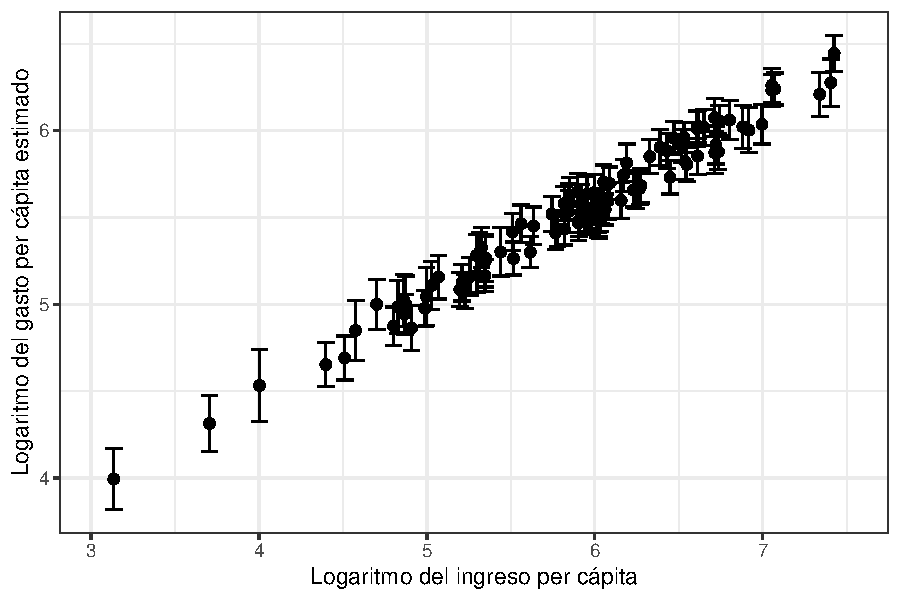
\includegraphics[width=0.65\linewidth,height=\textheight,keepaspectratio]{chapters/../figures/fig-prediction-intervals-1.pdf}

}

\caption{\label{fig-prediction-intervals}Estimaciones del logaritmo del
gasto per cápita e intervalos de confianza para los primeros 100 hogares
de la muestra}

\end{figure}%

Cuando el interés se centra en realizar predicciones para valores de las
covariables que se encuentran fuera del rango observado en la muestra,
la extrapolación puede incrementar la incertidumbre y hacer que los
resultados dependan en mayor medida de la forma funcional asumida. Para
una nueva unidad \(k\), con vector de covariables
\(\mathbf{x}_{k,\mathrm{nuevo}}\), la media condicional se define como

\[
\mu_{k,\mathrm{nuevo}}
=
E\left(
y_{k,\mathrm{nuevo}}
\mid
\mathbf{x}_{k,\mathrm{nuevo}}
\right)
=
\mathbf{x}'_{k,\mathrm{nuevo}}\boldsymbol{\beta},
\]

y su estimador está dado por

\[
\hat{\mu}_{k,\mathrm{nuevo}}
=
\mathbf{x}'_{k,\mathrm{nuevo}}
\hat{\boldsymbol{\beta}}.
\]

La varianza estimada de esta predicción es

\[
\widehat{Var}\left(
\hat{\mu}_{k,\mathrm{nuevo}}
\right)
=
\mathbf{x}'_{k,\mathrm{nuevo}}
\hat{\boldsymbol{\Sigma}}
\mathbf{x}_{k,\mathrm{nuevo}},
\]

donde
\(\hat{\boldsymbol{\Sigma}}=\widehat{Var}(\hat{\boldsymbol{\beta}})\)
corresponde a la matriz estimada de varianzas y covarianzas de los
coeficientes de regresión.

Si el interés fuera predecir \(y_{k,\mathrm{nuevo}}\) y no únicamente su
media condicional, sería necesario incorporar adicionalmente la
variabilidad residual del modelo. En ese caso,

\[
\widehat{Var}\left(
\hat{\mu}_{k,\mathrm{nuevo}} +
\varepsilon_{k,\mathrm{nuevo}}
\right)
=
\mathbf{x}'_{k,\mathrm{nuevo}}
\hat{\boldsymbol{\Sigma}}
\mathbf{x}_{k,\mathrm{nuevo}}
+
\hat{\sigma}^{2}_{y\mid x}.
\]

En donde \(\hat{\sigma}^{2}_{y\mid x}\) corresponde a la varianza
residual estimada; es decir, la parte de la variabilidad de la variable
respuesta que no es explicada por las covariables incluidas en el
modelo. La incorporación de este segundo componente es fundamental
cuando se desea predecir sobre unidades no observadas, ya que reconoce
explícitamente la existencia de variabilidad individual alrededor de la
media estimada.

En consecuencia, los intervalos de predicción suelen ser más amplios que
los intervalos de confianza para la media, reflejando una mayor
incertidumbre asociada a la predicción de valores individuales. De esta
manera, el intervalo de predicción para una nueva observación puede
expresarse como:

\begin{equation}\protect\phantomsection\label{eq-intervalo-prediccion}{
\mathbf{x}_{k}\hat{\boldsymbol{\beta}}
\pm
t_{\left(1-\frac{\alpha}{2},df\right)}
\sqrt{
\mathbf{x}_{k}^{\top}
\hat{\boldsymbol{\Sigma}} \
\mathbf{x}_{k}
+
\hat{\sigma}^2_{yx}
}
}\end{equation}

En el siguiente ejemplo se estima la media condicional del logaritmo del
gasto per cápita para un nuevo perfil de hogar y su intervalo de
confianza. El perfil corresponde a un hogar cuyo jefe tiene 45 años
(\texttt{Age}), es de sexo masculino (\texttt{Male}), reside en zona
urbana (\texttt{Urban}) de la región Norte (\texttt{North}) y tiene un
ingreso per cápita (\texttt{Income}) igual a 1600. Este perfil puede
definirse en \texttt{R} mediante el siguiente conjunto de datos:

\begin{Shaded}
\begin{Highlighting}[]
\NormalTok{new\_data }\OtherTok{\textless{}{-}} \FunctionTok{data.frame}\NormalTok{(}
  \AttributeTok{Income =} \DecValTok{1600}\NormalTok{,}
  \AttributeTok{Age =} \DecValTok{45}\NormalTok{,}
  \AttributeTok{Sex =} \StringTok{"Male"}\NormalTok{,}
  \AttributeTok{Zone =} \StringTok{"Urban"}\NormalTok{,}
  \AttributeTok{Region =} \StringTok{"North"}
\NormalTok{)}

\NormalTok{new\_prediction }\OtherTok{\textless{}{-}} \FunctionTok{predict}\NormalTok{(fit\_svy, }\AttributeTok{newdata =}\NormalTok{ new\_data, }\AttributeTok{type =} \StringTok{"link"}\NormalTok{)}
\NormalTok{new\_prediction}
\end{Highlighting}
\end{Shaded}

\begin{verbatim}
  link   SE
1 6.41 0.05
\end{verbatim}

\begin{Shaded}
\begin{Highlighting}[]
\NormalTok{new\_prediction\_interval }\OtherTok{\textless{}{-}} \FunctionTok{confint}\NormalTok{(new\_prediction)}
\NormalTok{new\_prediction\_interval}
\end{Highlighting}
\end{Shaded}

\begin{verbatim}
  2.5 % 97.5 %
1 6.305  6.507
\end{verbatim}

Para este perfil, la predicción del logaritmo del gasto per cápita es
6,406, con un intervalo de confianza del 95 \% entre 6,305 y 6,507. En
primer lugar, el objeto \texttt{new\_data} especifica los valores de las
covariables incluidas en el modelo. Posteriormente, la función
\texttt{predict()} calcula la predicción puntual asociada a dicha
observación. El argumento \texttt{newdata\ =\ new\_data} indica que la
predicción debe realizarse utilizando la nueva información suministrada,
mientras que \texttt{type\ =\ "link"} solicita el resultado en la escala
del predictor lineal. Finalmente, \texttt{confint()} aplicado al
resultado de \texttt{predict.svyglm()} produce un intervalo de confianza
para el valor medio estimado; no incorpora automáticamente el término
residual requerido para un intervalo de predicción individual.

\bookmarksetup{startatroot}

\chapter{Modelos lineales generalizados}\label{cap6}

Nelder y Wedderburn (\citeproc{ref-nelder1972generalized}{1972})
introdujeron los modelos lineales generalizados como un marco capaz de
integrar diversos métodos estadísticos ampliamente utilizados, como la
regresión logística, los modelos log-lineales para datos de conteo y
otros modelos avanzados de regresión para variables continuas.
Posteriormente, McCullagh y Nelder
(\citeproc{ref-McCullaghNelder1989}{1989}) sistematizaron esta
formulación, que permitió extender las herramientas de regresión más
allá de los escenarios en los que la variable respuesta sigue una
distribución normal. Cuando la variable de interés no es continua o los
supuestos del modelo lineal clásico no se satisfacen, los modelos
lineales generalizados constituyen una alternativa adecuada para modelar
las relaciones de interés.

La necesidad de esta generalización surge porque los modelos lineales
clásicos asumen, entre otras cosas, normalidad y homogeneidad de
varianza en los errores, condiciones que no se cumplen cuando se
analizan variables categóricas, proporciones o conteos. En este tipo de
situaciones, los modelos lineales generalizados ofrecen un marco
flexible para modelar adecuadamente la relación entre las variables
mediante la selección de una distribución de probabilidad apropiada para
la respuesta y una función de enlace que conecte la media de dicha
distribución con el predictor lineal.

Para ilustrar los modelos de este capítulo se utiliza la muestra
almacenada en \texttt{sample.rds}. El siguiente bloque carga las
librerías, define la condición de pobreza (\texttt{poor}), calcula el
tamaño del hogar (\texttt{household\_size}) contando los integrantes de
cada \texttt{HHID} y construye el diseño muestral. A partir de este
diseño se seleccionan las unidades de análisis correspondientes a cada
ejemplo.

\begin{Shaded}
\begin{Highlighting}[]
\FunctionTok{options}\NormalTok{(}\AttributeTok{digits =} \DecValTok{4}\NormalTok{)}
\FunctionTok{library}\NormalTok{(tidyverse)}
\FunctionTok{library}\NormalTok{(survey)}
\FunctionTok{library}\NormalTok{(srvyr)}
\FunctionTok{library}\NormalTok{(broom)}
\FunctionTok{library}\NormalTok{(jtools)}

\NormalTok{survey\_data }\OtherTok{\textless{}{-}} \FunctionTok{readRDS}\NormalTok{(}\StringTok{"../data/sample.rds"}\NormalTok{) }\SpecialCharTok{\%\textgreater{}\%}
  \FunctionTok{add\_count}\NormalTok{(HHID, }\AttributeTok{name =} \StringTok{"household\_size"}\NormalTok{) }\SpecialCharTok{\%\textgreater{}\%}
  \FunctionTok{mutate}\NormalTok{(}
    \AttributeTok{Stratum =} \FunctionTok{factor}\NormalTok{(Stratum),}
    \AttributeTok{poor =} \FunctionTok{factor}\NormalTok{(}
\NormalTok{      Poverty }\SpecialCharTok{!=} \StringTok{"NotPoor"}\NormalTok{,}
      \AttributeTok{levels =} \FunctionTok{c}\NormalTok{(}\ConstantTok{FALSE}\NormalTok{, }\ConstantTok{TRUE}\NormalTok{),}
      \AttributeTok{labels =} \FunctionTok{c}\NormalTok{(}\StringTok{"Not poor"}\NormalTok{, }\StringTok{"Poor"}\NormalTok{)}
\NormalTok{    )}
\NormalTok{  )}

\NormalTok{survey\_design }\OtherTok{\textless{}{-}}\NormalTok{ survey\_data }\SpecialCharTok{\%\textgreater{}\%}
  \FunctionTok{as\_survey\_design}\NormalTok{(}
    \AttributeTok{strata =}\NormalTok{ Stratum,}
    \AttributeTok{ids =}\NormalTok{ PSU,}
    \AttributeTok{weights =}\NormalTok{ wk,}
    \AttributeTok{nest =} \ConstantTok{TRUE}
\NormalTok{  )}
\end{Highlighting}
\end{Shaded}

\section{Modelo de regresión logística}\label{sec-logistica}

De acuerdo con McCullagh y Nelder
(\citeproc{ref-McCullaghNelder1989}{1989}) y Agresti
(\citeproc{ref-Agresti2019Intro}{2019}), cuando la variable de interés
es dicotómica, tomando valores de cero o uno, el modelo lineal clásico
no resulta adecuado debido a que puede generar predicciones fuera del
intervalo \((0,1)\). Para abordar estas limitaciones, el modelo de
regresión logística constituye uno de los modelos más utilizados para
analizar variables binarias. Además, en el contexto de encuestas de
hogares, la regresión logística puede emplearse para analizar la
asociación entre una condición de interés, como la pobreza, y
características sociodemográficas de los individuos o los hogares.

Considere, una variable dicotómica \(Y_k \in \{0,1\}\), cuya esperanza
es \(\theta_k=Pr(Y_k=1)\). El modelo de regresión logística relaciona
dicha probabilidad con un conjunto de variables explicativas mediante la
función de enlace logit, definida como

\begin{equation}\protect\phantomsection\label{eq-modelo-logistico}{
\log\left(\frac{\theta_k}{1-\theta_k}\right)
=
\beta_0+\beta_1x_{k1}+\cdots+\beta_px_{kp}
=\mathbf{x}_{k}\boldsymbol{\beta}
}\end{equation}

En donde \(\boldsymbol{\beta}\) es el vector de coeficientes de
regresión asociado a las covariables. Esta transformación logit
convierte el intervalo restringido de probabilidades \((0,1)\) en toda
la recta real, permitiendo modelar la relación entre la respuesta y las
variables auxiliares mediante un predictor lineal. De manera
equivalente, la probabilidad de éxito puede expresarse mediante la
siguiente relación:

\begin{equation}\protect\phantomsection\label{eq-probabilidad-logistica}{
\theta_k
=
Pr(Y_k = 1 \mid \mathbf{x}_k)
=
\frac{\exp(\mathbf{x}_k\boldsymbol{\beta})}
     {1+\exp(\mathbf{x}_k\boldsymbol{\beta})}
}\end{equation}

De manera equivalente, la probabilidad de que la unidad no presente la
característica de interés es
\(Pr(Y_k = 0 \mid \mathbf{x}_k) = 1-\theta_k\). Bajo esta
parametrización, cada coeficiente de \(\boldsymbol{\beta}\) representa
el efecto de una covariable sobre el logaritmo de la razón de
probabilidades de que ocurra el evento de interés, manteniendo
constantes las demás variables del modelo. Según Heeringa et~al.
(\citeproc{ref-HeeringaWestBerglund2017}{2017}), la estimación de los
parámetros puede realizarse mediante el enfoque de pseudo-máxima
verosimilitud. Este método, abordado con detalle en el
\hyperref[ap2]{segundo anexo}, incorpora los factores de expansión en la
función de verosimilitud convencional con el fin de obtener estimadores
consistentes respecto de la población objetivo. En este sentido, para
este modelo, la función de pseudo-verosimilitud para el modelo logístico
se define como

\[
PL(\boldsymbol{\beta})
=
\prod_{k}
\left[
\theta_{k}^{y_{k}}
\left\{
1-\theta_{k}
\right\}^{1-y_{k}}
\right]^{w_{k}}
\]

En donde el subíndice \(k\) representa una unidad observada de la
muestra. Asimismo, \(\theta_{k}\) denota la probabilidad de que la
unidad \(k\) de la UPM \(i\) en el estrato \(h\) presente la
característica de interés, \(y_{k}\) corresponde al valor observado de
la variable dicotómica para dicha unidad y \(w_{k}\) representa el
factor de expansión asociado a la observación.

Dado que la contribución de cada observación al proceso de estimación
está determinada por su respectivo factor de expansión, la función de
pseudo-verosimilitud refleja adecuadamente las características del
diseño complejo de la encuesta. Además, la maximización de esta función
resulta equivalente a maximizar su logaritmo, entonces el problema se
reduce a optimizar la siguiente función:

\begin{equation}\protect\phantomsection\label{eq-log-pseudoverosimilitud-logistica}{
\ell(\boldsymbol{\beta})
=
\sum_{k}
w_{k}
\left[
y_{k}\log(\theta_{k})
+
(1-y_{k})
\log(1-\theta_{k})
\right]
}\end{equation}

Esta expresión constituye la función objetivo utilizada por los
algoritmos de optimización numérica para obtener el estimador de los
parámetros del modelo. Es importante señalar que la función anterior no
corresponde a una verosimilitud en sentido estricto bajo el diseño
complejo de la encuesta. Por esta razón, se utiliza el término
\emph{pseudo-verosimilitud} y los estimadores obtenidos mediante su
maximización son conocidos como estimadores de pseudo-máxima
verosimilitud (\emph{Pseudo Maximum Likelihood Estimators}, PMLE).

De acuerdo con Molina y Skinner (\citeproc{ref-molina1992pseudo}{1992})
y Chambers y Skinner (\citeproc{ref-ChambersSkinner2003}{2003}), bajo
condiciones de regularidad, estos estimadores son consistentes y
asintóticamente normales, constituyendo la base de procedimientos de
inferencia para el análisis de datos de encuestas complejas. Como
explica Binder (\citeproc{ref-binder1983variances}{1983}) las varianzas
se estiman mediante técnicas de linealización de Taylor, las cuales
incorporan explícitamente las características del diseño complejo de
muestreo.

La matriz de varianzas y covarianzas de los parámetros estimados,
denotada por
\(\text{Var}(\hat{\boldsymbol{\beta}})=\boldsymbol{\Sigma}\), se obtiene
a partir de una aproximación lineal de las ecuaciones de estimación
alrededor del verdadero valor de los parámetros. Esta matriz describe la
precisión de los estimadores, ya que sus elementos diagonales
corresponden a las varianzas de cada coeficiente, mientras que los
elementos fuera de la diagonal representan las covarianzas entre pares
de coeficientes. Su estimación constituye la base para el cálculo de
errores estándar, la construcción de intervalos de confianza y la
realización de pruebas de hipótesis sobre los parámetros del modelo.

Para analizar los factores asociados a la condición de pobreza en la
encuesta de ejemplo, el siguiente código computacional ajusta un modelo
de regresión logística utilizando como variables explicativas la edad,
el sexo y la situación laboral del jefe, junto con el tamaño del hogar.
Estas características demográficas y laborales son habituales en el
análisis de los correlatos de la pobreza
(\citeproc{ref-Anyanwu2014}{Anyanwu 2014}). En este ejemplo, la pobreza
se define a partir del ingreso: \texttt{poor} toma la categoría
\texttt{Poor} para \texttt{Extreme} o \texttt{Relative}, y
\texttt{Not\ poor} para \texttt{NotPoor}. Se trabaja con una observación
por hogar, identificada mediante \texttt{PersonID\ ==\ "idPer01"}, y se
utiliza el factor de expansión \texttt{wk} del jefe, siguiendo la
convención descrita en la sección 3.1. Dado que los datos provienen de
una encuesta con diseño muestral complejo, la estimación se realiza
mediante la función \texttt{svyglm()} del paquete \texttt{survey},
especificando \texttt{family\ =\ quasibinomial()} para indicar que la
variable respuesta es dicotómica y que se utilizará la función de enlace
logit. Esta elección conserva los coeficientes y las varianzas basadas
en el diseño que se obtendrían con la familia binomial, y evita la
advertencia sobre respuestas ponderadas no enteras.

\begin{Shaded}
\begin{Highlighting}[]
\NormalTok{household\_design }\OtherTok{\textless{}{-}}\NormalTok{ survey\_design }\SpecialCharTok{\%\textgreater{}\%}
  \FunctionTok{filter}\NormalTok{(PersonID }\SpecialCharTok{==} \StringTok{"idPer01"}\NormalTok{) }\SpecialCharTok{\%\textgreater{}\%}
  \FunctionTok{mutate}\NormalTok{(}
    \AttributeTok{Sex =} \FunctionTok{factor}\NormalTok{(Sex, }\AttributeTok{levels =} \FunctionTok{c}\NormalTok{(}\StringTok{"Male"}\NormalTok{, }\StringTok{"Female"}\NormalTok{)),}
    \AttributeTok{Employment =} \FunctionTok{relevel}\NormalTok{(Employment, }\AttributeTok{ref =} \StringTok{"Employed"}\NormalTok{)}
\NormalTok{  )}

\NormalTok{logit\_model }\OtherTok{\textless{}{-}} \FunctionTok{svyglm}\NormalTok{(}
  \AttributeTok{formula =}\NormalTok{ poor }\SpecialCharTok{\textasciitilde{}}\NormalTok{ Age }\SpecialCharTok{+}\NormalTok{ Sex }\SpecialCharTok{+}\NormalTok{ Employment }\SpecialCharTok{+}\NormalTok{ household\_size,}
  \AttributeTok{family =} \FunctionTok{quasibinomial}\NormalTok{(),}
  \AttributeTok{design =}\NormalTok{ household\_design}
\NormalTok{)}
\end{Highlighting}
\end{Shaded}

En la especificación del modelo, el argumento
\texttt{formula\ =\ poor\ \textasciitilde{}\ Age\ +\ Sex\ +\ Employment\ +\ household\_size}
define la relación entre la variable respuesta \texttt{poor} y las
covariables incluidas en el predictor lineal (\texttt{Age},
\texttt{Sex}, \texttt{Employment} y \texttt{household\_size}). Para las
variables categóricas, la función genera automáticamente las variables
indicadoras correspondientes y estima sus efectos con respecto a una
categoría de referencia. Por su parte, el argumento
\texttt{design\ =\ household\_design} incorpora la información del
diseño muestral para los hogares seleccionados. Las categorías de
referencia son jefatura masculina y jefe ocupado. La muestra de análisis
contiene 696 hogares, de los cuales 225 son pobres; estos conteos
corresponden a observaciones muestrales, sin ponderar.

El objeto resultante, \texttt{logit\_model}, contiene los parámetros
estimados, sus medidas de precisión y las estadísticas necesarias para
realizar inferencia sobre la relación entre la condición de pobreza y
las variables explicativas consideradas en el modelo. El siguiente
código computacional organiza los coeficientes del modelo logístico, sus
medidas de precisión y sus exponenciales para presentarlos en la tabla.

\begin{Shaded}
\begin{Highlighting}[]
\NormalTok{logistic\_intervals\_table }\OtherTok{\textless{}{-}}\NormalTok{ logit\_results }\SpecialCharTok{\%\textgreater{}\%}
  \FunctionTok{mutate}\NormalTok{(}\AttributeTok{OR =} \FunctionTok{exp}\NormalTok{(estimate)) }\SpecialCharTok{\%\textgreater{}\%}
  \FunctionTok{select}\NormalTok{(}
\NormalTok{    term,}
\NormalTok{    estimate,}
\NormalTok{    std.error,}
\NormalTok{    p.value,}
\NormalTok{    conf.low,}
\NormalTok{    conf.high,}
\NormalTok{    OR}
\NormalTok{  )}

\NormalTok{logistic\_intervals\_table}
\end{Highlighting}
\end{Shaded}

{

\begin{longtable}[]{@{}
  >{\raggedright\arraybackslash}p{(\linewidth - 12\tabcolsep) * \real{0.2958}}
  >{\raggedleft\arraybackslash}p{(\linewidth - 12\tabcolsep) * \real{0.1549}}
  >{\raggedleft\arraybackslash}p{(\linewidth - 12\tabcolsep) * \real{0.0986}}
  >{\raggedleft\arraybackslash}p{(\linewidth - 12\tabcolsep) * \real{0.1127}}
  >{\raggedleft\arraybackslash}p{(\linewidth - 12\tabcolsep) * \real{0.1127}}
  >{\raggedleft\arraybackslash}p{(\linewidth - 12\tabcolsep) * \real{0.1127}}
  >{\raggedleft\arraybackslash}p{(\linewidth - 12\tabcolsep) * \real{0.1127}}@{}}

\caption{\label{tbl-ic-logistica}Intervalos de confianza al 95\% para
los parámetros del modelo logístico}

\tabularnewline

\toprule\noalign{}
\begin{minipage}[b]{\linewidth}\raggedright
Parámetro
\end{minipage} & \begin{minipage}[b]{\linewidth}\raggedleft
Estimación
\end{minipage} & \begin{minipage}[b]{\linewidth}\raggedleft
EE
\end{minipage} & \begin{minipage}[b]{\linewidth}\raggedleft
Valor p
\end{minipage} & \begin{minipage}[b]{\linewidth}\raggedleft
LI 95 \%
\end{minipage} & \begin{minipage}[b]{\linewidth}\raggedleft
LS 95 \%
\end{minipage} & \begin{minipage}[b]{\linewidth}\raggedleft
OR
\end{minipage} \\
\midrule\noalign{}
\endhead
\bottomrule\noalign{}
\endlastfoot
(Intercept) & -1.7217 & 0.4252 & 0.0001 & -2.5641 & -0.8794 & 0.1788 \\
Age & -0.0071 & 0.0078 & 0.3597 & -0.0225 & 0.0082 & 0.9929 \\
SexFemale & 0.4521 & 0.2468 & 0.0696 & -0.0368 & 0.9411 & 1.5717 \\
EmploymentUnemployed & 2.4380 & 0.7007 & 0.0007 & 1.0498 & 3.8262 &
11.4500 \\
EmploymentInactive & 0.1693 & 0.3272 & 0.6058 & -0.4788 & 0.8174 &
1.1845 \\
household\_size & 0.2990 & 0.0671 & 0.0000 & 0.1660 & 0.4319 & 1.3485 \\

\end{longtable}

}

Los resultados de la tabla~\ref{tbl-ic-logistica} muestran las
estimaciones de los coeficientes de regresión, sus exponenciales,
errores estándar, intervalos de confianza y valores-\emph{p}. Los
errores estándar y los límites de confianza se mantienen en la escala de
los coeficientes \(\beta\). En la regresión logística, \(\exp(\beta_j)\)
representa el \emph{odds ratio} asociado a una covariable, manteniendo
constantes las demás variables.

Manteniendo constantes las demás variables, el \emph{odds ratio} de
pobreza asociado a cada integrante adicional del hogar es 1.35, con un
intervalo de confianza del 95 \% entre 1.18 y 1.54. Al ser mayor que
uno, indica mayores \emph{odds} de pobreza asociadas con un mayor tamaño
del hogar. Asimismo, el \emph{odds ratio} de los hogares con jefe
desocupado respecto de aquellos con jefe ocupado es 11.45, con un
intervalo de confianza del 95 \% entre 2.86 y 45.89. Esta última
estimación presenta una incertidumbre considerable, pues solo se
observan 16 jefes desocupados. Los odds ratios superiores a uno indican
mayores odds de pobreza respecto de la comparación correspondiente, pero
no expresan cuántas veces mayor es esa probabilidad. Estas asociaciones
no establecen efectos causales.

La figura~\ref{fig-logistic-base} presenta la distribución de los
estimadores de los coeficientes de regresión. Se observa que los
intervalos de confianza asociados a la desocupación del jefe y al tamaño
del hogar no incluyen el valor cero, lo que proporciona evidencia de una
asociación estadísticamente significativa. En contraste, la edad, la
jefatura femenina y la inactividad del jefe presentan valores-\emph{p}
de 0.360, 0.070 y 0.606, respectivamente, por lo que no se encuentra
evidencia suficiente de asociación al nivel del 5 \% una vez controladas
las demás covariables incluidas en el modelo. El siguiente código
computacional genera el gráfico mediante \texttt{plot\_summs()} del
paquete \texttt{jtools} (\citeproc{ref-jtools2026}{Long 2026}) y las
geometrías horizontales de \texttt{ggstance}
(\citeproc{ref-ggstance2024}{Henry et~al. 2024}), para visualizar los
coeficientes y sus intervalos.

\begin{Shaded}
\begin{Highlighting}[]
\FunctionTok{library}\NormalTok{(ggstance)}
\FunctionTok{plot\_summs}\NormalTok{(}
\NormalTok{  logit\_model,}
  \AttributeTok{scale =} \ConstantTok{TRUE}\NormalTok{,}
  \AttributeTok{plot.distributions =} \ConstantTok{TRUE}
\NormalTok{)}
\end{Highlighting}
\end{Shaded}

\begin{figure}[H]

\centering{

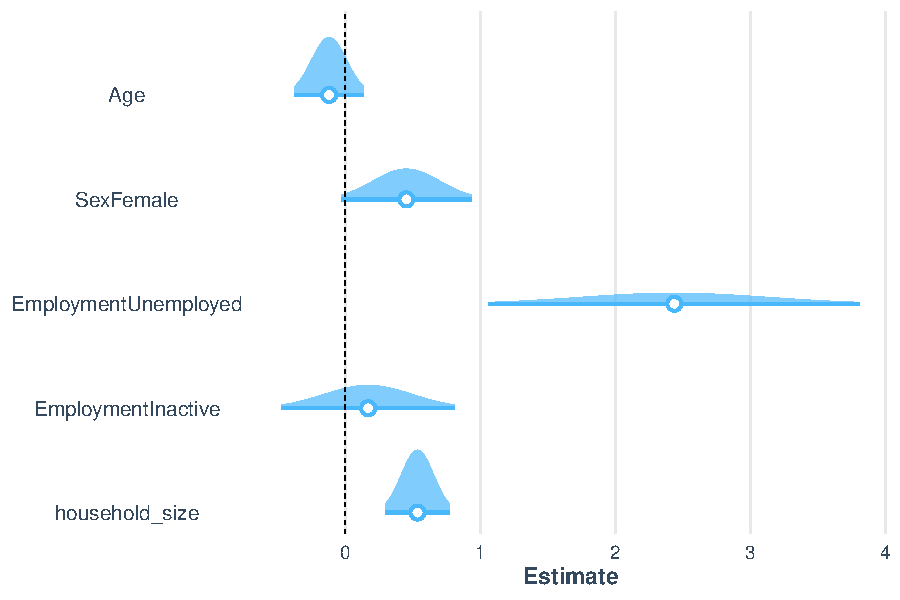
\includegraphics[width=0.8\linewidth,height=\textheight,keepaspectratio]{chapters/../figures/fig-logistic-base-1.pdf}

}

\caption{\label{fig-logistic-base}Distribución de los parámetros del
modelo logístico base}

\end{figure}%

El modelo puede ampliarse incorporando términos de interacción para
evaluar si el efecto de una variable explicativa depende de los valores
que toma otra. En este caso, se incluye una interacción entre el sexo
del jefe y el tamaño del hogar mediante el término
\texttt{Sex:household\_size}, con el objetivo de analizar si la relación
entre el número de integrantes y las \emph{odds} de pobreza es la misma
para hogares con jefatura masculina y femenina. Sin este término, el
modelo asume que la pendiente del tamaño del hogar sobre el logit de
pobreza es idéntica para ambos tipos de jefatura. En cambio, al
incorporar la interacción, se permite que dicha pendiente varíe,
capturando posibles diferencias en la forma en que el tamaño del hogar
se asocia con la pobreza en cada grupo. Los resultados del modelo
ajustado se presentan en la tabla~\ref{tbl-logistica-interaccion}. El
siguiente código computacional ajusta este modelo y reúne los
coeficientes, sus errores estándar, los intervalos de confianza y sus
exponenciales para facilitar la comparación.

\begin{Shaded}
\begin{Highlighting}[]
\NormalTok{interaction\_logit\_model }\OtherTok{\textless{}{-}} \FunctionTok{svyglm}\NormalTok{(}
  \AttributeTok{formula =}\NormalTok{ poor }\SpecialCharTok{\textasciitilde{}}\NormalTok{ Age }\SpecialCharTok{+}\NormalTok{ Sex }\SpecialCharTok{+}\NormalTok{ Employment }\SpecialCharTok{+}
\NormalTok{    household\_size }\SpecialCharTok{+}\NormalTok{ Sex}\SpecialCharTok{:}\NormalTok{household\_size,}
  \AttributeTok{family =} \FunctionTok{quasibinomial}\NormalTok{(),}
  \AttributeTok{design =}\NormalTok{ household\_design}
\NormalTok{)}
\end{Highlighting}
\end{Shaded}

\begin{Shaded}
\begin{Highlighting}[]
\NormalTok{interaction\_logistic\_coefficients\_table }\OtherTok{\textless{}{-}}\NormalTok{ interaction\_logit\_results }\SpecialCharTok{\%\textgreater{}\%}
  \FunctionTok{mutate}\NormalTok{(}\AttributeTok{OR =} \FunctionTok{exp}\NormalTok{(estimate)) }\SpecialCharTok{\%\textgreater{}\%}
  \FunctionTok{select}\NormalTok{(}
\NormalTok{    term,}
\NormalTok{    estimate,}
\NormalTok{    std.error,}
\NormalTok{    p.value,}
\NormalTok{    conf.low,}
\NormalTok{    conf.high,}
\NormalTok{    OR}
\NormalTok{  )}

\NormalTok{interaction\_logistic\_coefficients\_table}
\end{Highlighting}
\end{Shaded}

{

\begin{longtable}[]{@{}
  >{\raggedright\arraybackslash}p{(\linewidth - 12\tabcolsep) * \real{0.3333}}
  >{\raggedleft\arraybackslash}p{(\linewidth - 12\tabcolsep) * \real{0.1467}}
  >{\raggedleft\arraybackslash}p{(\linewidth - 12\tabcolsep) * \real{0.0933}}
  >{\raggedleft\arraybackslash}p{(\linewidth - 12\tabcolsep) * \real{0.1067}}
  >{\raggedleft\arraybackslash}p{(\linewidth - 12\tabcolsep) * \real{0.1067}}
  >{\raggedleft\arraybackslash}p{(\linewidth - 12\tabcolsep) * \real{0.1067}}
  >{\raggedleft\arraybackslash}p{(\linewidth - 12\tabcolsep) * \real{0.1067}}@{}}

\caption{\label{tbl-logistica-interaccion}Coeficientes del modelo
logístico con interacciones}

\tabularnewline

\toprule\noalign{}
\begin{minipage}[b]{\linewidth}\raggedright
Parámetro
\end{minipage} & \begin{minipage}[b]{\linewidth}\raggedleft
Estimación
\end{minipage} & \begin{minipage}[b]{\linewidth}\raggedleft
EE
\end{minipage} & \begin{minipage}[b]{\linewidth}\raggedleft
Valor p
\end{minipage} & \begin{minipage}[b]{\linewidth}\raggedleft
LI 95 \%
\end{minipage} & \begin{minipage}[b]{\linewidth}\raggedleft
LS 95 \%
\end{minipage} & \begin{minipage}[b]{\linewidth}\raggedleft
OR
\end{minipage} \\
\midrule\noalign{}
\endhead
\bottomrule\noalign{}
\endlastfoot
(Intercept) & -1.8438 & 0.4260 & 0.0000 & -2.6878 & -0.9998 & 0.1582 \\
Age & -0.0074 & 0.0079 & 0.3498 & -0.0230 & 0.0082 & 0.9926 \\
SexFemale & 0.7993 & 0.4825 & 0.1004 & -0.1567 & 1.7553 & 2.2240 \\
EmploymentUnemployed & 2.4724 & 0.6989 & 0.0006 & 1.0877 & 3.8571 &
11.8508 \\
EmploymentInactive & 0.1739 & 0.3292 & 0.5984 & -0.4784 & 0.8261 &
1.1899 \\
household\_size & 0.3304 & 0.0852 & 0.0002 & 0.1617 & 0.4991 & 1.3915 \\
SexFemale:household\_size & -0.0926 & 0.1288 & 0.4738 & -0.3477 & 0.1626
& 0.9116 \\

\end{longtable}

}

En ambas tablas, la exponencial del intercepto corresponde a las
\emph{odds} del perfil de referencia, no a un \emph{odds ratio}; en la
tabla con interacción, la exponencial de
\texttt{SexFemale:household\_size} representa la razón entre los
\emph{odds ratios} del tamaño del hogar de ambos tipos de jefatura.

Al incorporar la interacción entre sexo y tamaño del hogar, se permite
estimar una pendiente del tamaño del hogar diferente para cada tipo de
jefatura. Para los hogares con jefe hombre, el \emph{odds ratio}
asociado a un integrante adicional es 1.39; para los hogares con jefa
mujer, se obtiene combinando el coeficiente principal y el de
interacción, y es igual a 1.27. El coeficiente de interacción tiene un
valor-\emph{p} de 0.474. Estos resultados no aportan evidencia
suficiente de diferencias entre las pendientes al nivel del 5 \%; el
efecto principal del sexo, por su parte, corresponde a un tamaño del
hogar igual a cero, fuera del rango observado, por lo que no debe
interpretarse como una diferencia general entre jefaturas.

La figura~\ref{fig-logistic-comparison}, obtenida con el siguiente
código computacional, presenta una comparación de las estimaciones de
los coeficientes y sus respectivos intervalos de confianza para los
modelos con y sin interacción. Al incorporar el término de interacción,
cambia la interpretación de los efectos principales del sexo y del
tamaño del hogar, que pasan a ser condicionales a los valores de
referencia de la otra covariable. Los intervalos de confianza permiten
valorar la incertidumbre asociada a estas estimaciones y al coeficiente
de interacción.

\begin{Shaded}
\begin{Highlighting}[]
\FunctionTok{plot\_summs}\NormalTok{(}
\NormalTok{  interaction\_logit\_model,}
\NormalTok{  logit\_model,}
  \AttributeTok{scale =} \ConstantTok{TRUE}\NormalTok{,}
  \AttributeTok{plot.distributions =} \ConstantTok{TRUE}
\NormalTok{)}
\end{Highlighting}
\end{Shaded}

\begin{figure}[H]

\centering{

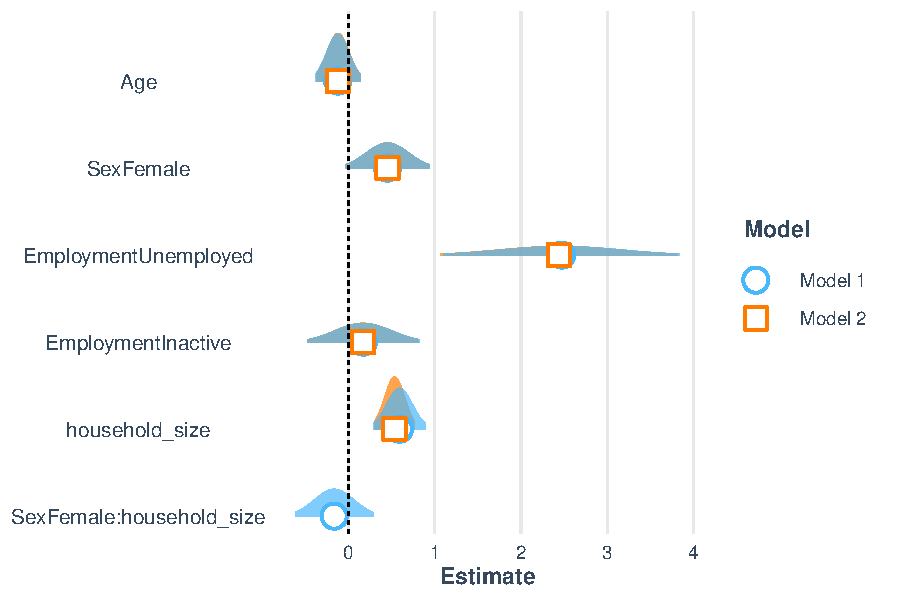
\includegraphics[width=0.7\linewidth,height=\textheight,keepaspectratio]{chapters/../figures/fig-logistic-comparison-1.pdf}

}

\caption{\label{fig-logistic-comparison}Comparación de los parámetros
del modelo logístico con y sin interacciones}

\end{figure}%

Los coeficientes del modelo permiten identificar la dirección de las
asociaciones entre las covariables y la condición de pobreza, pero no
indican directamente la probabilidad de pobreza de un hogar. Para
facilitar la interpretación, se estiman probabilidades predichas para
perfiles específicos. En el siguiente ejemplo se comparan hogares con
jefatura masculina o femenina, manteniendo iguales la edad del jefe, su
situación laboral y el tamaño del hogar.

\begin{Shaded}
\begin{Highlighting}[]
\NormalTok{prediction\_profiles }\OtherTok{\textless{}{-}} \FunctionTok{data.frame}\NormalTok{(}
  \AttributeTok{Age =} \FunctionTok{c}\NormalTok{(}\DecValTok{40}\NormalTok{, }\DecValTok{40}\NormalTok{),}
  \AttributeTok{Sex =} \FunctionTok{factor}\NormalTok{(}
    \FunctionTok{c}\NormalTok{(}\StringTok{"Male"}\NormalTok{, }\StringTok{"Female"}\NormalTok{),}
    \AttributeTok{levels =} \FunctionTok{levels}\NormalTok{(household\_design}\SpecialCharTok{$}\NormalTok{variables}\SpecialCharTok{$}\NormalTok{Sex)}
\NormalTok{  ),}
  \AttributeTok{Employment =} \FunctionTok{factor}\NormalTok{(}
    \FunctionTok{c}\NormalTok{(}\StringTok{"Employed"}\NormalTok{, }\StringTok{"Employed"}\NormalTok{),}
    \AttributeTok{levels =} \FunctionTok{levels}\NormalTok{(household\_design}\SpecialCharTok{$}\NormalTok{variables}\SpecialCharTok{$}\NormalTok{Employment)}
\NormalTok{  ),}
  \AttributeTok{household\_size =} \FunctionTok{c}\NormalTok{(}\DecValTok{4}\NormalTok{, }\DecValTok{4}\NormalTok{)}
\NormalTok{)}

\NormalTok{predictions }\OtherTok{\textless{}{-}} \FunctionTok{predict}\NormalTok{(}
\NormalTok{  logit\_model,}
  \AttributeTok{newdata =}\NormalTok{ prediction\_profiles,}
  \AttributeTok{type =} \StringTok{"response"}\NormalTok{,}
  \AttributeTok{se.fit =} \ConstantTok{TRUE}
\NormalTok{)}

\NormalTok{predicted\_probability }\OtherTok{\textless{}{-}} \FunctionTok{as.numeric}\NormalTok{(predictions)}
\NormalTok{standard\_error }\OtherTok{\textless{}{-}} \FunctionTok{as.numeric}\NormalTok{(}\FunctionTok{SE}\NormalTok{(predictions))}

\NormalTok{prediction\_table }\OtherTok{\textless{}{-}}\NormalTok{ prediction\_profiles }\SpecialCharTok{\%\textgreater{}\%}
  \FunctionTok{mutate}\NormalTok{(}
    \AttributeTok{predicted\_probability =}\NormalTok{ predicted\_probability,}
    \AttributeTok{standard\_error =}\NormalTok{ standard\_error,}
    \AttributeTok{lower\_95 =} \FunctionTok{pmax}\NormalTok{(}\DecValTok{0}\NormalTok{, predicted\_probability }\SpecialCharTok{{-}} \FloatTok{1.96} \SpecialCharTok{*}\NormalTok{ standard\_error),}
    \AttributeTok{upper\_95 =} \FunctionTok{pmin}\NormalTok{(}\DecValTok{1}\NormalTok{, predicted\_probability }\SpecialCharTok{+} \FloatTok{1.96} \SpecialCharTok{*}\NormalTok{ standard\_error)}
\NormalTok{  ) }\SpecialCharTok{\%\textgreater{}\%}
  \FunctionTok{select}\NormalTok{(}
\NormalTok{    Sex,}
\NormalTok{    Age,}
\NormalTok{    Employment,}
\NormalTok{    household\_size,}
\NormalTok{    predicted\_probability,}
\NormalTok{    lower\_95,}
\NormalTok{    upper\_95}
\NormalTok{  )}
\end{Highlighting}
\end{Shaded}

Los perfiles se fijan en 40 años, cuatro integrantes y jefe ocupado;
cuatro integrantes corresponde a la mediana del tamaño del hogar entre
los jefes seleccionados. Los niveles de \texttt{Sex} y
\texttt{Employment} se conservan tal como fueron definidos para el
modelo, de modo que las categorías de los perfiles coincidan con las
usadas durante la estimación. A partir de las probabilidades y sus
errores estándar se calculan límites aproximados del 95 \% en la escala
de probabilidad, restringidos al intervalo de cero a uno.

{

\begin{longtable}[]{@{}
  >{\raggedright\arraybackslash}p{(\linewidth - 12\tabcolsep) * \real{0.2151}}
  >{\raggedleft\arraybackslash}p{(\linewidth - 12\tabcolsep) * \real{0.0538}}
  >{\raggedright\arraybackslash}p{(\linewidth - 12\tabcolsep) * \real{0.1935}}
  >{\raggedleft\arraybackslash}p{(\linewidth - 12\tabcolsep) * \real{0.1828}}
  >{\raggedleft\arraybackslash}p{(\linewidth - 12\tabcolsep) * \real{0.1828}}
  >{\raggedleft\arraybackslash}p{(\linewidth - 12\tabcolsep) * \real{0.0860}}
  >{\raggedleft\arraybackslash}p{(\linewidth - 12\tabcolsep) * \real{0.0860}}@{}}

\caption{\label{tbl-probabilidades-perfiles-logistica}Probabilidades
predichas de pobreza para perfiles seleccionados}

\tabularnewline

\toprule\noalign{}
\begin{minipage}[b]{\linewidth}\raggedright
Sexo de la jefatura
\end{minipage} & \begin{minipage}[b]{\linewidth}\raggedleft
Edad
\end{minipage} & \begin{minipage}[b]{\linewidth}\raggedright
Situación laboral
\end{minipage} & \begin{minipage}[b]{\linewidth}\raggedleft
Tamaño del hogar
\end{minipage} & \begin{minipage}[b]{\linewidth}\raggedleft
Probabilidad (\%)
\end{minipage} & \begin{minipage}[b]{\linewidth}\raggedleft
LI 95 \%
\end{minipage} & \begin{minipage}[b]{\linewidth}\raggedleft
LS 95 \%
\end{minipage} \\
\midrule\noalign{}
\endhead
\bottomrule\noalign{}
\endlastfoot
Male & 40 & Employed & 4 & 30.76 & 24.34 & 37.17 \\
Female & 40 & Employed & 4 & 41.11 & 32.41 & 49.82 \\

\end{longtable}

}

La tabla~\ref{tbl-probabilidades-perfiles-logistica} presenta las
probabilidades e intervalos como porcentajes. Para el perfil de jefatura
masculina, la probabilidad predicha de pobreza es 30.8 \% (IC aproximado
del 95 \%: 24.3--37.2 \%); para el de jefatura femenina, es 41.1 \% (IC
aproximado del 95 \%: 32.4--49.8 \%). La diferencia descriptiva es de
10.4 puntos porcentuales. Son predicciones condicionadas a los perfiles
definidos, no proporciones generales de pobreza; esta diferencia por sí
sola tampoco constituye una prueba de significación estadística.

\section{Modelo de regresión multinomial}\label{sec-multinomial}

En las encuestas de hogares es frecuente encontrar variables de
respuesta con más de dos categorías, como la situación laboral, cuyos
posibles estados incluyen tres categorías: empleado, desempleado e
inactivo. Cuando estas categorías son mutuamente excluyentes y no poseen
un orden natural, la regresión logística multinomial ofrece una
herramienta adecuada para modelar su relación con un conjunto de
covariables y puede entenderse como una extensión de la regresión
logística binaria (\citeproc{ref-McCullaghNelder1989}{McCullagh y Nelder
1989}; \citeproc{ref-Agresti2019Intro}{Agresti 2019}).

Este modelo permite estimar la probabilidad de pertenecer a cada
categoría de la variable respuesta en función de variables explicativas
de naturaleza continua o categórica. Su aplicación requiere que las
categorías de respuesta sean exhaustivas y mutuamente excluyentes y que
no exista multicolinealidad severa entre las covariables. Además, para
las covariables continuas, se asume que existe una relación lineal entre
estas y el logaritmo de las razones de probabilidades (\emph{log-odds})
de cada categoría respecto a una categoría de referencia.

El modelo logístico multinomial especifica la probabilidad
\(\theta_{k(j)}\) de que la unidad \(k\) pertenezca a la categoría
\(j\), con \(j=1,\ldots,J\), dado el vector de covariables
\(\mathbf{x}_k\), mediante la siguiente expresión:

\begin{equation}\protect\phantomsection\label{eq-probabilidad-multinomial}{
Pr(Y_{k} = j \mid \mathbf{x}_{k})
=
\theta_{k(j)}
=
\frac{\exp(\mathbf{x}_{k}\boldsymbol{\beta}_j)}
     {\sum_{l=1}^{J} \exp(\mathbf{x}_{k}\boldsymbol{\beta}_l)}
}\end{equation}

En donde \(\boldsymbol{\beta}_j\) es el vector de coeficientes de
regresión para la \(j\)-ésima categoría. Para que el modelo sea
identificable, debe fijarse el vector de una categoría de referencia en
cero; de ese modo, la expresión produce \(J-1\) conjuntos de
coeficientes estimables. Aunque existen parametrizaciones alternativas
que facilitan la interpretación de los parámetros, esta formulación
expresa directamente las probabilidades de pertenencia a cada categoría.
Con una categoría de referencia, cada conjunto de coeficientes describe
cómo cambian, en escala logarítmica, las razones entre la probabilidad
de pertenecer a una categoría y la probabilidad de pertenecer a la
categoría de referencia (\emph{log-odds} relativos a la referencia).

Según Heeringa et~al. (\citeproc{ref-HeeringaWestBerglund2017}{2017}),
la estimación de los parámetros del modelo se realiza mediante el
enfoque de pseudo-máxima verosimilitud, definida de la siguiente manera:

\[
PL(\boldsymbol{\beta} \mid \mathbf{X}) =
\prod_{k}
\left\{
\prod_{j=1}^{J}
\theta_{k(j)}^{y_{k(j)}}
\right\}^{w_{k}}
\]

En donde \(k\) representa las unidades de observación pertenecientes a
la muestra compleja. Asimismo, \(y_{k(j)}\) es una variable indicadora
que toma el valor de uno cuando dicha unidad pertenece a la categoría
\(j\) y cero en caso contrario, y \(w_{k}\) corresponde al factor de
expansión asociado a la unidad observada. Por conveniencia matemática y
computacional, la estimación de los parámetros se realiza a partir de la
pseudo-logverosimilitud, \(\ell(\boldsymbol{\beta})\), cuya maximización
conduce a los mismos estimadores que la pseudo-verosimilitud original.

\begin{equation}\protect\phantomsection\label{eq-log-pseudoverosimilitud-multinomial}{
\ell(\boldsymbol{\beta})
=
\sum_{k} w_k
\sum_{j=1}^{J}
y_{k(j)}
\log(\theta_{k(j)})
}\end{equation}

La inferencia estadística para los parámetros de interés se basa en
estimaciones de varianza obtenidas mediante técnicas de linealización de
Taylor que incorporan explícitamente las características del diseño
muestral complejo, permitiendo calcular errores estándar, intervalos de
confianza y pruebas de hipótesis apropiados para datos de encuestas.
Bajo condiciones regulares, los estimadores obtenidos mediante este
procedimiento son consistentes y asintóticamente normales
(\citeproc{ref-molina1992pseudo}{Molina y Skinner 1992};
\citeproc{ref-binder1983variances}{Binder 1983}).

Como referencia inicial, el siguiente código computacional estima la
distribución por estado de empleo entre las personas de 15 años o más.
Los resultados se presentan en la tabla~\ref{tbl-prop-empleo-15}.

\begin{Shaded}
\begin{Highlighting}[]
\NormalTok{employment\_proportion }\OtherTok{\textless{}{-}}\NormalTok{ survey\_design }\SpecialCharTok{\%\textgreater{}\%}
  \FunctionTok{filter}\NormalTok{(Age }\SpecialCharTok{\textgreater{}=} \DecValTok{15}\NormalTok{) }\SpecialCharTok{\%\textgreater{}\%}
  \FunctionTok{group\_by}\NormalTok{(Employment) }\SpecialCharTok{\%\textgreater{}\%}
  \FunctionTok{summarise}\NormalTok{(}
    \AttributeTok{proportion =} \FunctionTok{survey\_mean}\NormalTok{(}\AttributeTok{vartype =} \FunctionTok{c}\NormalTok{(}\StringTok{"se"}\NormalTok{, }\StringTok{"ci"}\NormalTok{))}
\NormalTok{  )}

\NormalTok{employment\_proportions\_table }\OtherTok{\textless{}{-}}\NormalTok{ employment\_proportion}

\NormalTok{employment\_proportions\_table}
\end{Highlighting}
\end{Shaded}

{

\begin{longtable}[]{@{}lrrrr@{}}

\caption{\label{tbl-prop-empleo-15}Proporción estimada de personas por
estado de empleo (de 15 años o más)}

\tabularnewline

\toprule\noalign{}
Condición de actividad & Proporción & EE & LI 95 \% & LS 95 \% \\
\midrule\noalign{}
\endhead
\bottomrule\noalign{}
\endlastfoot
Unemployed & 0.0429 & 0.0071 & 0.0288 & 0.0571 \\
Inactive & 0.3840 & 0.0152 & 0.3539 & 0.4142 \\
Employed & 0.5731 & 0.0140 & 0.5453 & 0.6008 \\

\end{longtable}

}

De acuerdo con Lumley (\citeproc{ref-svyVGAM2026}{2026}), para modelar
una variable de respuesta multinomial se emplea la función
\texttt{svy\_vglm()} del paquete \texttt{svyVGAM}, que permite ajustar
modelos de regresión multinomial incorporando explícitamente las
características del diseño complejo de la encuesta. En este ejemplo, se
especifica un modelo donde la condición de actividad se explica en
función de la edad, el sexo y la zona de residencia. A diferencia de los
modelos multinomiales convencionales, \texttt{svy\_vglm()} calcula las
varianzas de los estimadores considerando la complejidad del diseño
muestral.

Las siguientes líneas de código ajustan un modelo de regresión
multinomial sobre las personas de 15 años o más, susceptibles de ser
clasificadas en una de las tres categorías de \texttt{Employment}. Note
que el argumento
\texttt{family\ =\ multinomial(refLevel\ =\ "Unemployed")} define un
modelo logístico multinomial tomando la categoría \texttt{Unemployed}
como referencia. Bajo esta especificación, se estiman de manera
simultánea los logaritmos de las razones de probabilidades
(\emph{log-odds}) entre cada una de las categorías de
\texttt{Employment} y la categoría de referencia. Los parámetros se
obtienen mediante pseudo-máxima verosimilitud, incorporando los factores
de expansión de la encuesta en la función objetivo.

\begin{Shaded}
\begin{Highlighting}[]
\FunctionTok{library}\NormalTok{(svyVGAM)}

\NormalTok{survey\_design\_15 }\OtherTok{\textless{}{-}}\NormalTok{ survey\_design }\SpecialCharTok{\%\textgreater{}\%}
  \FunctionTok{filter}\NormalTok{(Age }\SpecialCharTok{\textgreater{}=} \DecValTok{15}\NormalTok{)}

\NormalTok{multinomial\_model }\OtherTok{\textless{}{-}} \FunctionTok{svy\_vglm}\NormalTok{(}
  \AttributeTok{formula =}\NormalTok{ Employment }\SpecialCharTok{\textasciitilde{}}\NormalTok{ Age }\SpecialCharTok{+}\NormalTok{ Sex }\SpecialCharTok{+}\NormalTok{ Zone,}
  \AttributeTok{design =}\NormalTok{ survey\_design\_15,}
  \AttributeTok{crit =} \StringTok{"coef"}\NormalTok{,}
  \AttributeTok{family =} \FunctionTok{multinomial}\NormalTok{(}\AttributeTok{refLevel =} \StringTok{"Unemployed"}\NormalTok{)}
\NormalTok{)}
\end{Highlighting}
\end{Shaded}

La tabla~\ref{tbl-multinomial-coef} presenta los coeficientes estimados
del modelo logístico multinomial, tomando la categoría
\texttt{Unemployed} como referencia. Los errores estándar y los
intervalos de confianza del 95 \% se expresan en la escala de los
coeficientes \(\beta\). Para el intercepto, la exponencial es la razón
de probabilidades del perfil de referencia, no una comparación entre
perfiles. Los resultados muestran que la edad tiene una asociación
positiva y estadísticamente significativa con las probabilidades
relativas de pertenecer a las categorías \texttt{Inactive} y
\texttt{Employed} frente a \texttt{Unemployed}. Asimismo, la variable
\texttt{SexMale} presenta coeficientes negativos y significativos,
indicando que, manteniendo constantes la edad y la zona, los hombres
tienen menores razones relativas de estar \texttt{Inactive} o
\texttt{Employed} frente a estar \texttt{Unemployed} que las mujeres.
Por el contrario, la variable de zona de residencia no muestra efectos
estadísticamente significativos al nivel convencional del 5\%. El
siguiente código computacional prepara los coeficientes del modelo
multinomial para la tabla: asigna etiquetas a las categorías de
respuesta y calcula la razón de riesgo relativo como la exponencial del
coeficiente.

\begin{Shaded}
\begin{Highlighting}[]
\NormalTok{multinomial\_coefficients\_table }\OtherTok{\textless{}{-}}\NormalTok{ multinomial\_results }\SpecialCharTok{\%\textgreater{}\%}
  \FunctionTok{mutate}\NormalTok{(}
    \AttributeTok{y.level =} \FunctionTok{recode}\NormalTok{(y.level, }\StringTok{\textasciigrave{}}\AttributeTok{1}\StringTok{\textasciigrave{}} \OtherTok{=} \StringTok{"Inactive"}\NormalTok{, }\StringTok{\textasciigrave{}}\AttributeTok{2}\StringTok{\textasciigrave{}} \OtherTok{=} \StringTok{"Employed"}\NormalTok{),}
    \AttributeTok{RRR =} \FunctionTok{exp}\NormalTok{(estimate)}
\NormalTok{  ) }\SpecialCharTok{\%\textgreater{}\%}
  \FunctionTok{select}\NormalTok{(}
\NormalTok{    y.level,}
\NormalTok{    term,}
\NormalTok{    estimate,}
\NormalTok{    std.error,}
\NormalTok{    p.value,}
\NormalTok{    conf.low,}
\NormalTok{    conf.high,}
\NormalTok{    RRR}
\NormalTok{  )}

\NormalTok{multinomial\_coefficients\_table}
\end{Highlighting}
\end{Shaded}

{

\begin{longtable}[]{@{}
  >{\raggedright\arraybackslash}p{(\linewidth - 14\tabcolsep) * \real{0.1389}}
  >{\raggedright\arraybackslash}p{(\linewidth - 14\tabcolsep) * \real{0.1667}}
  >{\raggedleft\arraybackslash}p{(\linewidth - 14\tabcolsep) * \real{0.1528}}
  >{\raggedleft\arraybackslash}p{(\linewidth - 14\tabcolsep) * \real{0.0972}}
  >{\raggedleft\arraybackslash}p{(\linewidth - 14\tabcolsep) * \real{0.1111}}
  >{\raggedleft\arraybackslash}p{(\linewidth - 14\tabcolsep) * \real{0.1111}}
  >{\raggedleft\arraybackslash}p{(\linewidth - 14\tabcolsep) * \real{0.1111}}
  >{\raggedleft\arraybackslash}p{(\linewidth - 14\tabcolsep) * \real{0.1111}}@{}}

\caption{\label{tbl-multinomial-coef}Coeficientes estimados del modelo
de regresión multinomial}

\tabularnewline

\toprule\noalign{}
\begin{minipage}[b]{\linewidth}\raggedright
Categoría
\end{minipage} & \begin{minipage}[b]{\linewidth}\raggedright
Parámetro
\end{minipage} & \begin{minipage}[b]{\linewidth}\raggedleft
Estimación
\end{minipage} & \begin{minipage}[b]{\linewidth}\raggedleft
EE
\end{minipage} & \begin{minipage}[b]{\linewidth}\raggedleft
Valor p
\end{minipage} & \begin{minipage}[b]{\linewidth}\raggedleft
LI 95 \%
\end{minipage} & \begin{minipage}[b]{\linewidth}\raggedleft
LS 95 \%
\end{minipage} & \begin{minipage}[b]{\linewidth}\raggedleft
RRR
\end{minipage} \\
\midrule\noalign{}
\endhead
\bottomrule\noalign{}
\endlastfoot
Inactive & (Intercept) & 2.5565 & 0.5500 & 0.0000 & 1.4785 & 3.6344 &
12.8902 \\
Inactive & Age & 0.0221 & 0.0104 & 0.0343 & 0.0016 & 0.0425 & 1.0223 \\
Inactive & SexMale & -2.1851 & 0.3166 & 0.0000 & -2.8057 & -1.5646 &
0.1125 \\
Inactive & ZoneUrban & -0.2536 & 0.4045 & 0.5307 & -1.0464 & 0.5392 &
0.7760 \\
Employed & (Intercept) & 2.3063 & 0.4614 & 0.0000 & 1.4020 & 3.2107 &
10.0377 \\
Employed & Age & 0.0181 & 0.0088 & 0.0398 & 0.0008 & 0.0355 & 1.0183 \\
Employed & SexMale & -0.5783 & 0.2766 & 0.0365 & -1.1203 & -0.0362 &
0.5609 \\
Employed & ZoneUrban & 0.0392 & 0.3605 & 0.9135 & -0.6674 & 0.7457 &
1.0399 \\

\end{longtable}

}

La columna RRR (\emph{relative risk ratio}), se calcula como
\(\exp(\beta)\) e indica el factor de cambio en la razón entre la
probabilidad de la categoría indicada y la de referencia, manteniendo
constantes las demás covariables. En la tabla, el RRR de
\texttt{SexMale} para la categoría \texttt{Employed} es 0.56.
Manteniendo constantes la edad y la zona, la razón entre la probabilidad
de estar empleado y la de estar desempleado para los hombres equivale a
ese valor multiplicado por la razón correspondiente para las mujeres.
Esto representa una razón relativa aproximadamente 43.9 \% menor.

De acuerdo con Warnes et~al. (\citeproc{ref-gtools2025}{2023}) y Solt y
Hu (\citeproc{ref-dotwhisker2025}{2025}), la
figura~\ref{fig-multinomial-ci}, obtenida con el siguiente código
computacional, muestra los intervalos de confianza de los coeficientes
estimados para cada ecuación del modelo multinomial. Se usa
\texttt{gtools::stars.pval()} para codificar la significación
estadística, y la visualización se construye con
\texttt{dotwhisker::dwplot()}, lo que permite comparar coeficientes e
intervalos en una escala común. Las covariables cuyos intervalos no
incluyen el valor cero presentan evidencia de asociación estadística
significativa con la variable respuesta, mientras que aquellos cuyos
intervalos contienen el cero no muestran efectos significativos al nivel
de confianza considerado.

\begin{Shaded}
\begin{Highlighting}[]
\NormalTok{multinomial\_results }\SpecialCharTok{\%\textgreater{}\%}
  \FunctionTok{mutate}\NormalTok{(}
    \AttributeTok{model =} \FunctionTok{if\_else}\NormalTok{(y.level }\SpecialCharTok{==} \DecValTok{1}\NormalTok{, }\StringTok{"Inactive"}\NormalTok{, }\StringTok{"Employed"}\NormalTok{),}
    \AttributeTok{sig =}\NormalTok{ gtools}\SpecialCharTok{::}\FunctionTok{stars.pval}\NormalTok{(p.value)}
\NormalTok{  ) }\SpecialCharTok{\%\textgreater{}\%}
\NormalTok{  dotwhisker}\SpecialCharTok{::}\FunctionTok{dwplot}\NormalTok{(}
    \AttributeTok{dodge\_size =} \FloatTok{0.3}\NormalTok{,}
    \AttributeTok{vline =} \FunctionTok{geom\_vline}\NormalTok{(}
      \AttributeTok{xintercept =} \DecValTok{0}\NormalTok{,}
      \AttributeTok{colour =} \StringTok{"grey60"}\NormalTok{,}
      \AttributeTok{linetype =} \DecValTok{2}
\NormalTok{    )}
\NormalTok{  ) }\SpecialCharTok{+}
  \FunctionTok{guides}\NormalTok{(}\AttributeTok{color =} \FunctionTok{guide\_legend}\NormalTok{(}\AttributeTok{reverse =} \ConstantTok{TRUE}\NormalTok{)) }\SpecialCharTok{+}
  \FunctionTok{theme\_bw}\NormalTok{() }\SpecialCharTok{+}
  \FunctionTok{theme}\NormalTok{(}\AttributeTok{legend.position =} \StringTok{"top"}\NormalTok{)}
\end{Highlighting}
\end{Shaded}

\begin{figure}[H]

\centering{

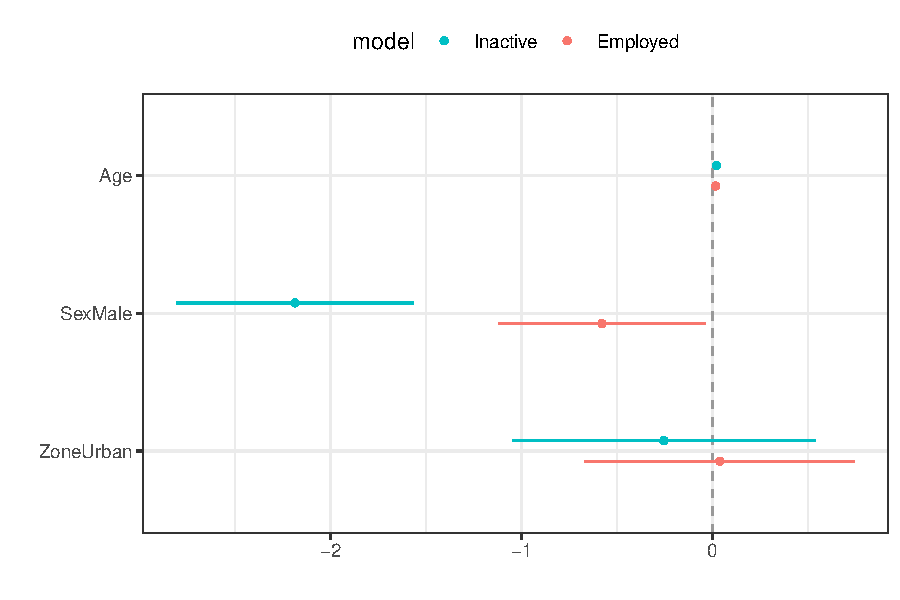
\includegraphics[width=0.75\linewidth,height=\textheight,keepaspectratio]{chapters/../figures/fig-multinomial-ci-1.pdf}

}

\caption{\label{fig-multinomial-ci}Intervalos de confianza para los
coeficientes del modelo multinomial}

\end{figure}%

\section{Modelo de regresión Gamma}\label{sec-gamma}

La regresión Gamma constituye una extensión de los modelos lineales
generalizados adecuada para variables respuesta continuas, estrictamente
positivas y cuya variabilidad aumenta con la media
(\citeproc{ref-McCullaghNelder1989}{McCullagh y Nelder 1989}). Este
comportamiento es frecuente en variables económicas y sociales, como los
ingresos de los hogares o los gastos en consumo.

Si \(Y_{k}\), la variable de interés observada para la unidad \(k\),
sigue una distribución Gamma con media \(\mu_{k}\) y parámetro de
dispersión \(\phi\), el modelo relaciona el valor esperado de la
variable respuesta con un conjunto de covariables mediante una función
de enlace. El enlace logarítmico es una opción frecuente y garantiza
predicciones positivas, aunque el enlace canónico de la familia Gamma es
el inverso. En este caso, el modelo se expresa como

\begin{equation}\protect\phantomsection\label{eq-modelo-gamma-log}{
\log(\mu_{k})
=
\mathbf{x}_{k}\boldsymbol{\beta}
}\end{equation}

En donde \(\mathbf{x}_{k}\) corresponde al vector de variables
explicativas asociado a la unidad observada y \(\boldsymbol{\beta}\) es
el vector de parámetros desconocidos del modelo. De forma equivalente,
se tiene que:

\[
\mu_{k}
= E(Y_{k}\mid \mathbf{x}_{k})
=
\exp(\mathbf{x}_{k}\boldsymbol{\beta}),
\]

Con el enlace logarítmico, cada parámetro puede interpretarse como el
efecto de una covariable sobre el logaritmo de la media esperada, de
manera que \(\exp(\beta_j)\) representa el cambio multiplicativo
asociado a un incremento unitario en la covariable correspondiente,
manteniendo constantes las demás variables del modelo. Bajo la
distribución Gamma, la función de densidad condicional de \(Y_{k}\)
puede escribirse como

\[
f(y_{k}\mid \mu_{k},\phi)
=
\frac{1}
{\Gamma(1/\phi)
(\phi\mu_{k})^{1/\phi}}
y_{k}^{\frac{1}{\phi}-1}
\exp\left(
-\frac{y_{k}}
{\phi\mu_{k}}
\right),
\qquad y_{k}>0,
\]

donde \(\Gamma(\cdot)\) denota la función Gamma y \(\phi\) representa el
parámetro de dispersión. Bajo el enfoque de inferencia basado en
pseudo-máxima verosimilitud, la función objetivo que se optimiza para
obtener los estimadores de los parámetros del modelo está dada por

\[
\ell(\boldsymbol{\beta},\phi)
=
\sum_{k}
w_{k}
\log
\left[
f(y_{k}\mid\mu_{k},\phi)
\right]
\]

En donde \(k\) representa las unidades de observación de la muestra y
\(w_k\) corresponde al factor de expansión asociado a cada una de ellas.
Esta función define el criterio de optimización utilizado para estimar
los parámetros del modelo bajo el enfoque de pseudo-máxima
verosimilitud, descrito para encuestas complejas por Chambers y Skinner
(\citeproc{ref-ChambersSkinner2003}{2003}).

El siguiente código computacional ajusta, mediante \texttt{svyglm()}, un
modelo de regresión Gamma para el ingreso per cápita del hogar
(\texttt{Income}), incorporando el diseño complejo de la encuesta
conservado en el objeto \texttt{household\_design}. La unidad de
análisis es el hogar, con una observación por hogar identificada
mediante \texttt{PersonID\ ==\ "idPer01"}, siguiendo la convención
utilizada en el modelo logístico. La muestra de análisis contiene 696
hogares; las categorías de referencia son jefatura masculina y zona
rural. El modelo utiliza como variables explicativas el gasto per cápita
del hogar (\texttt{Expenditure}), la edad del jefe de hogar
(\texttt{Age}), su sexo (\texttt{Sex}) y la zona de residencia
(\texttt{Zone}). Asimismo, se especifica una función de enlace
logarítmica, garantizando predicciones positivas y permitiendo
interpretar los efectos de las variables explicativas en términos
multiplicativos sobre el ingreso per cápita esperado. Finalmente, se
reúnen los coeficientes, sus medidas de precisión y los factores
multiplicativos correspondientes para presentarlos en la
tabla~\ref{tbl-gamma-coeficientes}.

\begin{Shaded}
\begin{Highlighting}[]
\NormalTok{gamma\_model }\OtherTok{\textless{}{-}} \FunctionTok{svyglm}\NormalTok{(}
  \AttributeTok{formula =}\NormalTok{ Income }\SpecialCharTok{\textasciitilde{}}\NormalTok{ Expenditure }\SpecialCharTok{+}\NormalTok{ Age }\SpecialCharTok{+}\NormalTok{ Sex }\SpecialCharTok{+}\NormalTok{ Zone,}
  \AttributeTok{design =}\NormalTok{ household\_design,}
  \AttributeTok{family =} \FunctionTok{Gamma}\NormalTok{(}\AttributeTok{link =} \StringTok{"log"}\NormalTok{)}
\NormalTok{)}
\end{Highlighting}
\end{Shaded}

\begin{Shaded}
\begin{Highlighting}[]
\NormalTok{gamma\_results }\OtherTok{\textless{}{-}}\NormalTok{ broom}\SpecialCharTok{::}\FunctionTok{tidy}\NormalTok{(}
\NormalTok{  gamma\_model,}
  \AttributeTok{conf.int =} \ConstantTok{TRUE}\NormalTok{,}
  \AttributeTok{conf.level =} \FloatTok{0.95}
\NormalTok{)}
\NormalTok{gamma\_coefficients\_table }\OtherTok{\textless{}{-}}\NormalTok{ gamma\_results }\SpecialCharTok{\%\textgreater{}\%}
  \FunctionTok{mutate}\NormalTok{(}\AttributeTok{factor =} \FunctionTok{exp}\NormalTok{(estimate)) }\SpecialCharTok{\%\textgreater{}\%}
  \FunctionTok{select}\NormalTok{(}
\NormalTok{    term,}
\NormalTok{    estimate,}
\NormalTok{    std.error,}
\NormalTok{    p.value,}
\NormalTok{    conf.low,}
\NormalTok{    conf.high,}
\NormalTok{    factor}
\NormalTok{  )}

\NormalTok{gamma\_coefficients\_table}
\end{Highlighting}
\end{Shaded}

{

\begin{longtable}[]{@{}
  >{\raggedright\arraybackslash}p{(\linewidth - 12\tabcolsep) * \real{0.1579}}
  >{\raggedleft\arraybackslash}p{(\linewidth - 12\tabcolsep) * \real{0.1447}}
  >{\raggedleft\arraybackslash}p{(\linewidth - 12\tabcolsep) * \real{0.0921}}
  >{\raggedleft\arraybackslash}p{(\linewidth - 12\tabcolsep) * \real{0.1053}}
  >{\raggedleft\arraybackslash}p{(\linewidth - 12\tabcolsep) * \real{0.1053}}
  >{\raggedleft\arraybackslash}p{(\linewidth - 12\tabcolsep) * \real{0.1053}}
  >{\raggedleft\arraybackslash}p{(\linewidth - 12\tabcolsep) * \real{0.2895}}@{}}

\caption{\label{tbl-gamma-coeficientes}Coeficientes del modelo Gamma
para el ingreso per cápita de los hogares}

\tabularnewline

\toprule\noalign{}
\begin{minipage}[b]{\linewidth}\raggedright
Parámetro
\end{minipage} & \begin{minipage}[b]{\linewidth}\raggedleft
Estimación
\end{minipage} & \begin{minipage}[b]{\linewidth}\raggedleft
EE
\end{minipage} & \begin{minipage}[b]{\linewidth}\raggedleft
Valor p
\end{minipage} & \begin{minipage}[b]{\linewidth}\raggedleft
LI 95 \%
\end{minipage} & \begin{minipage}[b]{\linewidth}\raggedleft
LS 95 \%
\end{minipage} & \begin{minipage}[b]{\linewidth}\raggedleft
Factor multiplicativo
\end{minipage} \\
\midrule\noalign{}
\endhead
\bottomrule\noalign{}
\endlastfoot
(Intercept) & 5.4392 & 0.1257 & 0.0000 & 5.1902 & 5.6882 & 230.2624 \\
Expenditure & 0.0019 & 0.0001 & 0.0000 & 0.0017 & 0.0021 & 1.0019 \\
Age & 0.0002 & 0.0014 & 0.8634 & -0.0026 & 0.0030 & 1.0002 \\
SexFemale & -0.1521 & 0.0785 & 0.0551 & -0.3077 & 0.0034 & 0.8589 \\
ZoneUrban & 0.1606 & 0.0747 & 0.0336 & 0.0127 & 0.3085 & 1.1742 \\

\end{longtable}

}

Dado que el modelo utiliza un enlace logarítmico, la columna Factor
multiplicativo muestra \(\exp(\beta)\), es decir, el cambio
multiplicativo en el ingreso esperado asociado a una unidad adicional de
una covariable, manteniendo constantes las demás; para una variable
categórica, la comparación se realiza respecto de su categoría de
referencia. El cambio porcentual correspondiente es
\(100[\exp(\beta)-1]\). Para el intercepto, la exponencial representa la
media esperada del perfil de referencia. Los errores estándar y los
intervalos de confianza del 95 \% permanecen en la escala de los
coeficientes \(\beta\). El coeficiente asociado al gasto per cápita es
positivo y estadísticamente significativo (valor-\emph{p}:
\textless0.001): manteniendo constantes las demás covariables, un dólar
adicional de gasto per cápita se asocia con un aumento aproximado del
0,187 \% en el ingreso per cápita esperado. La residencia en zona urbana
también presenta una asociación positiva y estadísticamente
significativa (valor-\emph{p}: 0.0336), con un ingreso per cápita
esperado aproximadamente 17,4 \% mayor que en la zona rural, manteniendo
constantes el gasto per cápita, la edad y el sexo del jefe. En cambio,
no se encuentra evidencia suficiente de asociación para la edad del jefe
(valor-\emph{p}: 0.863) ni para la jefatura femenina respecto de la
masculina (valor-\emph{p}: 0.0551) al nivel del 5 \%. Estas asociaciones
no establecen efectos causales.

\bookmarksetup{startatroot}

\chapter{Modelos multinivel}\label{cap7}

Los modelos multinivel, también conocidos como modelos jerárquicos, son
una técnica estadística diseñada para el análisis de datos con
estructura jerárquica, como los que provienen de encuestas de hogares,
en donde las unidades de observación no son independientes entre sí
(\citeproc{ref-goldstein2011multilevel}{Goldstein 2011};
\citeproc{ref-rabehesketh2012multilevel}{Rabe-Hesketh y Skrondal 2012}).
Los individuos pertenecen a hogares, los hogares se ubican en áreas
geográficas específicas (UPMs) y estas, a su vez, forman parte de
unidades territoriales más amplias (estratos o dominios). Como
consecuencia, las observaciones que comparten un mismo contexto suelen
presentar características más similares entre sí que aquellas
pertenecientes a contextos diferentes. Esta estructura de dependencia
viola uno de los supuestos fundamentales de los modelos de regresión
convencionales y puede conducir a estimaciones ineficientes e
inferencias incorrectas.

A diferencia de los modelos de regresión convencionales, los modelos
multinivel reconocen que las observaciones pueden estar agrupadas en
distintos niveles y que cada uno de ellos puede contribuir a explicar la
variabilidad observada. En consecuencia, permiten representar
simultáneamente los efectos asociados a las características de las
unidades de análisis y aquellos derivados del entorno o contexto en el
que estas se encuentran. Esta formulación resulta especialmente útil
cuando se busca estudiar fenómenos determinados tanto por factores
individuales como por características de los hogares, comunidades o
áreas geográficas.

Como explica Snijders y Bosker (\citeproc{ref-snijders2011}{2011}), otra
característica relevante de los modelos multinivel es que permiten
cuantificar la proporción de la variabilidad asociada a cada nivel de
agrupación presente en los datos. Mientras los efectos fijos resumen la
relación promedio entre la variable respuesta y las covariables
incluidas en el modelo, los efectos aleatorios representan las
diferencias sistemáticas entre los grupos que no son explicadas por
dichas covariables. Gracias a esta estructura, es posible modelar
explícitamente la dependencia entre observaciones pertenecientes a un
mismo grupo y obtener inferencias más adecuadas cuando los datos
presentan organización jerárquica.

De acuerdo con Gelman y Hill (\citeproc{ref-gelman2006data}{2006}), el
desarrollo teórico y metodológico de los modelos multinivel ha sido
ampliamente documentado en la literatura de muestreo. Sus fundamentos
conceptuales, estrategias de estimación y aplicaciones en contextos
sociales y demográficos se encuentran consolidados en distintas
referencias especializadas. Por otra parte, la comparación entre
enfoques de estimación para modelos jerárquicos permite evaluar
diferencias entre los métodos basados en máxima verosimilitud y los
enfoques bayesianos (\citeproc{ref-browne2006comparison}{Browne y Draper
2006}).

Según Merlo et~al. (\citeproc{ref-merlo2006brief}{2006}), en el ámbito
de la epidemiología social, los modelos multinivel resultan útiles para
estudiar fenómenos contextuales, mostrando cómo factores asociados al
entorno pueden contribuir a explicar desigualdades en salud y otros
resultados de interés poblacional. Además, como advierten Pfeffermann
et~al. (\citeproc{ref-pfeffermann1998weighting}{1998}) y Carle
(\citeproc{ref-Carle2009}{2009}), es necesario distinguir entre la
jerarquía sustantiva que se desea modelar y la estructura del diseño
muestral: una UPM, un estrato de diseño o un dominio no constituye
automáticamente un contexto intercambiable susceptible de representarse
mediante un efecto aleatorio. Esa decisión requiere una justificación
conceptual y suficiente información en cada grupo.

\section{Motivación}\label{sec-motivacionMult}

Para iniciar este capítulo, se cargan las bibliotecas \texttt{tidyverse}
para la manipulación de datos y la generación de gráficos, y
\texttt{lme4} para la estimación de modelos multinivel
(\citeproc{ref-BatesEtAl2015}{Bates et~al. 2015}). Asimismo, se importa
la base de datos que será utilizada a lo largo de los ejemplos. Los
títulos matemáticos de algunas figuras se formatean con
\texttt{latex2exp}, llamado de forma explícita en el código.

\begin{Shaded}
\begin{Highlighting}[]
\FunctionTok{library}\NormalTok{(tidyverse)}
\FunctionTok{library}\NormalTok{(lme4)}

\NormalTok{survey\_data }\OtherTok{\textless{}{-}} \FunctionTok{readRDS}\NormalTok{(}\StringTok{"../data/sample.rds"}\NormalTok{) }\SpecialCharTok{\%\textgreater{}\%}
  \FunctionTok{add\_count}\NormalTok{(HHID, }\AttributeTok{name =} \StringTok{"household\_size"}\NormalTok{) }\SpecialCharTok{\%\textgreater{}\%}
  \FunctionTok{filter}\NormalTok{(PersonID }\SpecialCharTok{==} \StringTok{"idPer01"}\NormalTok{)}


\NormalTok{survey\_data }\OtherTok{\textless{}{-}}\NormalTok{ survey\_data }\SpecialCharTok{\%\textgreater{}\%}
  \FunctionTok{mutate}\NormalTok{(}
    \AttributeTok{poor =} \FunctionTok{ifelse}\NormalTok{(Poverty }\SpecialCharTok{!=} \StringTok{"NotPoor"}\NormalTok{, }\DecValTok{1}\NormalTok{, }\DecValTok{0}\NormalTok{),}
    \AttributeTok{log\_expenditure =} \FunctionTok{log}\NormalTok{(Expenditure),}
    \AttributeTok{log\_income =} \FunctionTok{log}\NormalTok{(Income)}
\NormalTok{  )}
\end{Highlighting}
\end{Shaded}

La base de análisis contiene 696 hogares, representados por una
observación seleccionada mediante \texttt{PersonID\ ==\ "idPer01"}. El
factor de expansión \texttt{wk} de la persona principal se utiliza como
aproximación al peso del hogar, siguiendo la convención y las
limitaciones descritas en la sección 3.1. Antes de seleccionar ese
registro, se calcula el tamaño del hogar (\texttt{household\_size}) con
\texttt{add\_count(HHID)}, contando a todos sus integrantes. Las
variables \texttt{Income} y \texttt{Expenditure} corresponden al ingreso
y al gasto mensual per cápita del hogar; \texttt{Age} registra la edad
de la persona principal. La selección deja un único registro por hogar.
En esta base, el ingreso y el gasto son finitos y positivos, lo que
permite obtener sus logaritmos naturales mediante \texttt{log()}. Los
nombres y las categorías de las variables se conservan en inglés.

A partir de esta base, el capítulo desarrolla dos aplicaciones. La
primera estudia la relación entre el logaritmo del gasto
(\texttt{log\_expenditure}) y el logaritmo del ingreso
(\texttt{log\_income}): la sección de motivación presenta la relación
bivariada y los modelos lineales multinivel incorporan posteriormente la
edad como control. La escala logarítmica permite interpretar la
pendiente del ingreso como una elasticidad: un aumento del 1 \% en el
ingreso se asocia con un cambio aproximado del \(\beta\) \% en el gasto
típico, expresado mediante su media geométrica condicional, manteniendo
constantes las demás covariables y el efecto del estrato. Además,
comprime la escala de los valores elevados, aunque no garantiza el
cumplimiento de los supuestos del modelo. La segunda aplicación utiliza
modelos logísticos multinivel para estudiar la asociación entre el
logaritmo del gasto y la condición de pobreza, controlando por el tamaño
del hogar.

Con fines ilustrativos, los ajustes iniciales de esta sección utilizan
los tres estratos con menor número de hogares. La base
\texttt{plot\_data} permite mostrar las limitaciones de los ajustes
independientes en grupos pequeños y se utiliza después para visualizar
los modelos multinivel. Estos últimos se estiman con los 696 hogares de
todos los estratos, contenidos en \texttt{survey\_data}. La selección de
tres estratos sirve para ilustrar el método y no representa por sí sola
a la población. El siguiente código computacional prepara la selección
de hogares y estratos que se utilizará en las ilustraciones.

\begin{Shaded}
\begin{Highlighting}[]
\NormalTok{plot\_data }\OtherTok{\textless{}{-}}\NormalTok{ survey\_data }\SpecialCharTok{\%\textgreater{}\%}
  \FunctionTok{select}\NormalTok{(HHID, Stratum) }\SpecialCharTok{\%\textgreater{}\%}
  \FunctionTok{distinct}\NormalTok{() }\SpecialCharTok{\%\textgreater{}\%}
  \FunctionTok{group\_by}\NormalTok{(Stratum) }\SpecialCharTok{\%\textgreater{}\%}
  \FunctionTok{tally}\NormalTok{() }\SpecialCharTok{\%\textgreater{}\%}
  \FunctionTok{arrange}\NormalTok{(n) }\SpecialCharTok{\%\textgreater{}\%}
  \FunctionTok{select}\NormalTok{(}\SpecialCharTok{{-}}\NormalTok{n) }\SpecialCharTok{\%\textgreater{}\%}
  \FunctionTok{slice}\NormalTok{(}\DecValTok{1}\SpecialCharTok{:}\DecValTok{3}\NormalTok{L) }\SpecialCharTok{\%\textgreater{}\%}
  \FunctionTok{inner\_join}\NormalTok{(survey\_data, }\AttributeTok{by =} \StringTok{"Stratum"}\NormalTok{) }\SpecialCharTok{\%\textgreater{}\%}
  \FunctionTok{select}\NormalTok{(Income, Expenditure, log\_income, log\_expenditure,}
\NormalTok{         household\_size, Age, Stratum, Sex, Region, Zone, poor)}
\end{Highlighting}
\end{Shaded}

Como punto de partida, se ajusta un modelo de regresión lineal
convencional que relaciona el logaritmo del gasto per cápita de los
hogares con el logaritmo de su ingreso per cápita, ignorando
temporalmente la estructura jerárquica de los datos. Bajo esta
especificación, se asume que todas las observaciones son independientes
y que la relación entre los logaritmos del ingreso y del gasto es
homogénea para todos los hogares, independientemente del estrato al que
pertenezcan. La figura~\ref{fig-regression-simple}, obtenida con el
siguiente código computacional, presenta la recta de regresión estimada
junto con los datos observados.

\begin{Shaded}
\begin{Highlighting}[]
\NormalTok{simple\_model }\OtherTok{\textless{}{-}} \FunctionTok{lm}\NormalTok{(log\_expenditure }\SpecialCharTok{\textasciitilde{}}\NormalTok{ log\_income, }\AttributeTok{data =}\NormalTok{ plot\_data)}

\FunctionTok{ggplot}\NormalTok{(}\AttributeTok{data =}\NormalTok{ plot\_data, }\FunctionTok{aes}\NormalTok{(}\AttributeTok{y =}\NormalTok{ log\_expenditure, }\AttributeTok{x =}\NormalTok{ log\_income)) }\SpecialCharTok{+}
  \FunctionTok{geom\_point}\NormalTok{() }\SpecialCharTok{+}
  \FunctionTok{labs}\NormalTok{(}\AttributeTok{x =} \StringTok{"Logaritmo del ingreso per cápita"}\NormalTok{,}
       \AttributeTok{y =} \StringTok{"Logaritmo del gasto per cápita"}\NormalTok{) }\SpecialCharTok{+}
  \FunctionTok{geom\_smooth}\NormalTok{(}
    \AttributeTok{formula =}\NormalTok{ y }\SpecialCharTok{\textasciitilde{}}\NormalTok{ x,}
    \AttributeTok{method =} \StringTok{"lm"}\NormalTok{,}
    \AttributeTok{se =} \ConstantTok{FALSE}
\NormalTok{  ) }\SpecialCharTok{+}
  \FunctionTok{theme}\NormalTok{(}
    \AttributeTok{legend.position =} \StringTok{"none"}\NormalTok{,}
    \AttributeTok{plot.title =} \FunctionTok{element\_text}\NormalTok{(}\AttributeTok{hjust =} \FloatTok{0.5}\NormalTok{)}
\NormalTok{  )}
\end{Highlighting}
\end{Shaded}

\begin{figure}[H]

\centering{

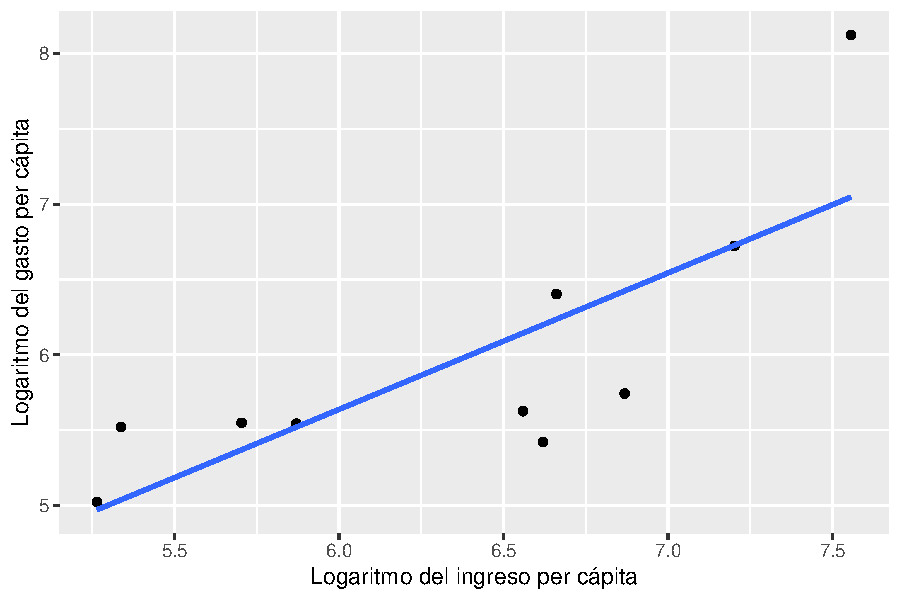
\includegraphics[width=0.7\linewidth,height=\textheight,keepaspectratio]{chapters/../figures/fig-regression-simple-1.pdf}

}

\caption{\label{fig-regression-simple}Modelo de regresión lineal simple
para el logaritmo del gasto en función del logaritmo del ingreso (sin
considerar estratos)}

\end{figure}%

Teniendo en cuenta los coeficientes de regresión estimados en la
tabla~\ref{tbl-motivation-models}, en este ajuste inicial un ingreso 1
\% mayor se asocia con un gasto aproximadamente 0,906 \% mayor. Como
explica Finch et~al. (\citeproc{ref-finch2019multilevel}{2019}), si bien
este modelo resulta útil como referencia inicial, sus supuestos suelen
ser poco realistas en el contexto de encuestas de hogares. En
particular, la independencia entre observaciones puede verse
comprometida cuando los hogares pertenecen a estratos que comparten
características socioeconómicas, demográficas o geográficas similares.
Asimismo, es posible que los niveles promedio del logaritmo del gasto
difieran sistemáticamente entre estratos, aun cuando la relación entre
los logaritmos del ingreso y del gasto sea semejante. Ignorar esta
estructura jerárquica puede conducir a estimaciones incorrectas de los
errores estándar y, en consecuencia, a inferencias estadísticas poco
confiables.

Para incorporar gradualmente la estructura jerárquica de los datos, el
siguiente código computacional ajusta un modelo que permite que cada
estrato tenga su propio intercepto, mientras mantiene una pendiente
común para todas las observaciones. Esta especificación resulta útil
para visualizar cómo los niveles promedio del logaritmo del gasto pueden
diferir entre estratos, aun cuando la relación entre los logaritmos del
ingreso y del gasto se considere constante. Los coeficientes se
utilizarán para trazar las rectas de regresión.

\begin{Shaded}
\begin{Highlighting}[]
\NormalTok{beta\_1 }\OtherTok{\textless{}{-}} \FunctionTok{coef}\NormalTok{(simple\_model)[}\DecValTok{2}\NormalTok{]}
\NormalTok{model\_coef }\OtherTok{\textless{}{-}}\NormalTok{ plot\_data }\SpecialCharTok{\%\textgreater{}\%}
  \FunctionTok{group\_by}\NormalTok{(Stratum) }\SpecialCharTok{\%\textgreater{}\%}
  \FunctionTok{summarise}\NormalTok{(}
    \AttributeTok{beta\_0 =} \FunctionTok{mean}\NormalTok{(log\_expenditure }\SpecialCharTok{{-}}\NormalTok{ beta\_1 }\SpecialCharTok{*}\NormalTok{ log\_income)}
\NormalTok{  ) }\SpecialCharTok{\%\textgreater{}\%}
  \FunctionTok{mutate}\NormalTok{(}\AttributeTok{beta\_1 =}\NormalTok{ beta\_1)}

\NormalTok{common\_slope\_coefficients }\OtherTok{\textless{}{-}}\NormalTok{ model\_coef}
\end{Highlighting}
\end{Shaded}

De esta manera, el modelo introduce una primera fuente de heterogeneidad
entre grupos y permite apreciar las limitaciones del modelo de regresión
simple presentado anteriormente, el cual asumía una única recta de
regresión para toda la población. La
figura~\ref{fig-intercept-by-stratum}, obtenida con el siguiente código
computacional, presenta las rectas de regresión con interceptos
diferenciados por estrato.

\begin{Shaded}
\begin{Highlighting}[]
\FunctionTok{ggplot}\NormalTok{(}
  \AttributeTok{data =}\NormalTok{ plot\_data,}
  \FunctionTok{aes}\NormalTok{(}
    \AttributeTok{y =}\NormalTok{ log\_expenditure,}
    \AttributeTok{x =}\NormalTok{ log\_income,}
    \AttributeTok{colour =}\NormalTok{ Stratum}
\NormalTok{  )}
\NormalTok{) }\SpecialCharTok{+}
  \FunctionTok{geom\_point}\NormalTok{() }\SpecialCharTok{+}
  \FunctionTok{labs}\NormalTok{(}\AttributeTok{x =} \StringTok{"Logaritmo del ingreso per cápita"}\NormalTok{,}
       \AttributeTok{y =} \StringTok{"Logaritmo del gasto per cápita"}\NormalTok{) }\SpecialCharTok{+}
  \FunctionTok{geom\_abline}\NormalTok{(}
    \AttributeTok{data =}\NormalTok{ model\_coef,}
    \AttributeTok{mapping =} \FunctionTok{aes}\NormalTok{(}
      \AttributeTok{slope =}\NormalTok{ beta\_1,}
      \AttributeTok{intercept =}\NormalTok{ beta\_0,}
      \AttributeTok{colour =}\NormalTok{ Stratum}
\NormalTok{    )}
\NormalTok{  ) }\SpecialCharTok{+}
  \FunctionTok{theme}\NormalTok{(}
    \AttributeTok{legend.position =} \StringTok{"none"}\NormalTok{,}
    \AttributeTok{plot.title =} \FunctionTok{element\_text}\NormalTok{(}\AttributeTok{hjust =} \FloatTok{0.5}\NormalTok{)}
\NormalTok{  )}
\end{Highlighting}
\end{Shaded}

\begin{figure}[H]

\centering{

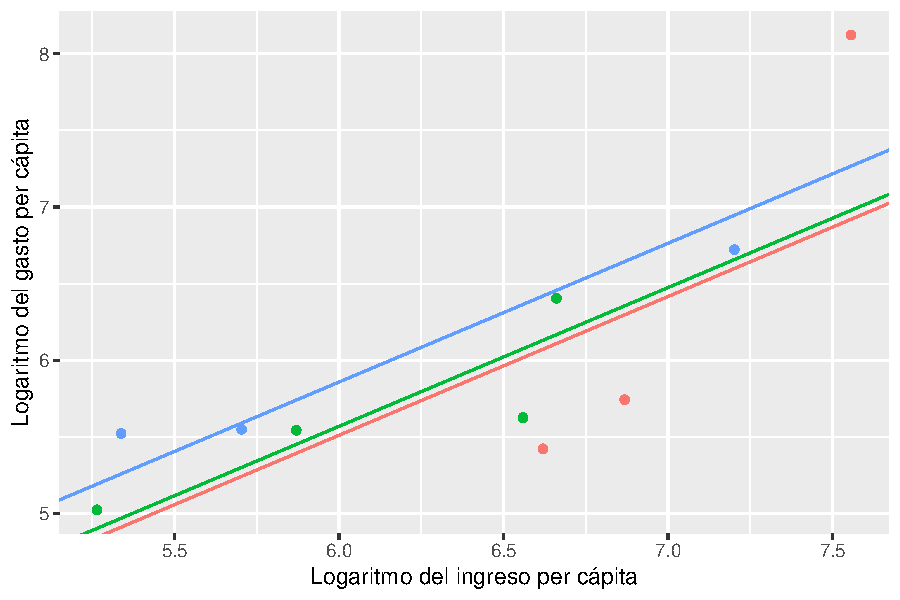
\includegraphics[width=0.7\linewidth,height=\textheight,keepaspectratio]{chapters/../figures/fig-intercept-by-stratum-1.pdf}

}

\caption{\label{fig-intercept-by-stratum}Modelo con intercepto
específico por estrato y pendiente común}

\end{figure}%

Como muestra la tabla~\ref{tbl-motivation-models}, los interceptos
difieren entre estratos, mientras que la elasticidad es común. Dentro de
cada estrato, un ingreso 1 \% mayor se asocia con un gasto
aproximadamente 0,906 \% mayor, manteniendo constantes las demás
variables incluidas en el modelo. Así, los estratos pueden diferir en el
nivel del gasto, pero comparten su respuesta proporcional al ingreso.
Como siguiente paso, se considera una especificación alternativa en la
que todos los estratos comparten un mismo intercepto en la escala
logarítmica, pero se permite que la relación entre los logaritmos del
ingreso y del gasto varíe entre estratos mediante pendientes específicas
para cada uno de ellos.

\begin{Shaded}
\begin{Highlighting}[]
\NormalTok{beta\_0 }\OtherTok{\textless{}{-}} \FunctionTok{coef}\NormalTok{(simple\_model)[}\DecValTok{1}\NormalTok{]}
\NormalTok{model\_coef }\OtherTok{\textless{}{-}}\NormalTok{ plot\_data }\SpecialCharTok{\%\textgreater{}\%}
  \FunctionTok{group\_by}\NormalTok{(Stratum) }\SpecialCharTok{\%\textgreater{}\%}
  \FunctionTok{summarise}\NormalTok{(}
    \AttributeTok{beta\_1 =} \FunctionTok{coef}\NormalTok{(}\FunctionTok{lm}\NormalTok{(}\FunctionTok{I}\NormalTok{(log\_expenditure }\SpecialCharTok{{-}}\NormalTok{ beta\_0) }\SpecialCharTok{\textasciitilde{}} \DecValTok{0} \SpecialCharTok{+}\NormalTok{ log\_income))[[}\DecValTok{1}\NormalTok{]]}
\NormalTok{  ) }\SpecialCharTok{\%\textgreater{}\%}
  \FunctionTok{mutate}\NormalTok{(}\AttributeTok{beta\_0 =}\NormalTok{ beta\_0)}

\NormalTok{common\_intercept\_coefficients }\OtherTok{\textless{}{-}}\NormalTok{ model\_coef}
\end{Highlighting}
\end{Shaded}

Bajo esta especificación, las diferencias entre estratos se manifiestan
en la intensidad de la asociación entre los logaritmos del ingreso y del
gasto, manteniendo fijo el intercepto. La
figura~\ref{fig-slope-by-stratum}, obtenida con el siguiente código
computacional, permite visualizar estas diferencias en las trayectorias
de regresión estimadas para cada estrato.

\begin{Shaded}
\begin{Highlighting}[]
\FunctionTok{ggplot}\NormalTok{(}
  \AttributeTok{data =}\NormalTok{ plot\_data,}
  \FunctionTok{aes}\NormalTok{(}
    \AttributeTok{y =}\NormalTok{ log\_expenditure,}
    \AttributeTok{x =}\NormalTok{ log\_income,}
    \AttributeTok{colour =}\NormalTok{ Stratum}
\NormalTok{  )}
\NormalTok{) }\SpecialCharTok{+}
  \FunctionTok{geom\_point}\NormalTok{() }\SpecialCharTok{+}
  \FunctionTok{labs}\NormalTok{(}\AttributeTok{x =} \StringTok{"Logaritmo del ingreso per cápita"}\NormalTok{,}
       \AttributeTok{y =} \StringTok{"Logaritmo del gasto per cápita"}\NormalTok{) }\SpecialCharTok{+}
  \FunctionTok{geom\_abline}\NormalTok{(}
    \AttributeTok{data =}\NormalTok{ model\_coef,}
    \AttributeTok{mapping =} \FunctionTok{aes}\NormalTok{(}
      \AttributeTok{slope =}\NormalTok{ beta\_1,}
      \AttributeTok{intercept =}\NormalTok{ beta\_0,}
      \AttributeTok{colour =}\NormalTok{ Stratum}
\NormalTok{    )}
\NormalTok{  ) }\SpecialCharTok{+}
  \FunctionTok{theme}\NormalTok{(}
    \AttributeTok{legend.position =} \StringTok{"none"}\NormalTok{,}
    \AttributeTok{plot.title =} \FunctionTok{element\_text}\NormalTok{(}\AttributeTok{hjust =} \FloatTok{0.5}\NormalTok{)}
\NormalTok{  )}
\end{Highlighting}
\end{Shaded}

\begin{figure}[H]

\centering{

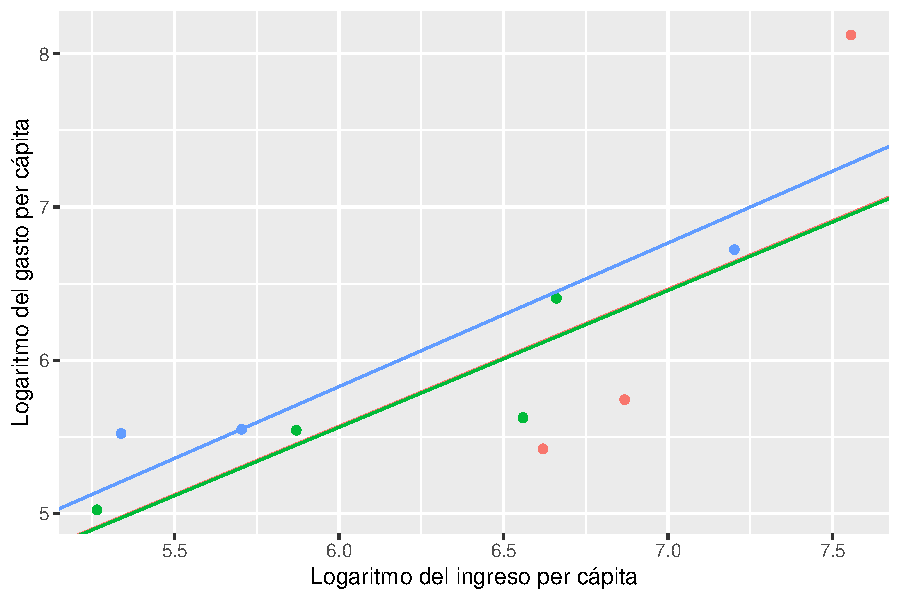
\includegraphics[width=0.7\linewidth,height=\textheight,keepaspectratio]{chapters/../figures/fig-slope-by-stratum-1.pdf}

}

\caption{\label{fig-slope-by-stratum}Modelo con pendiente específica por
estrato e intercepto común}

\end{figure}%

Con intercepto común y pendientes específicas, cada estrato tiene una
elasticidad distinta, como se observa en la
tabla~\ref{tbl-motivation-models}. Las estimaciones van de 0,893 a
0,937. Por ejemplo, en el estrato idStrt039, un ingreso 1 \% mayor se
asocia con un gasto aproximadamente 0,894 \% mayor, manteniendo
constantes las demás variables incluidas en el modelo.

Finalmente, se considera la especificación más flexible de las
presentadas hasta el momento, permitiendo que tanto el intercepto del
logaritmo del gasto como la relación entre los logaritmos del ingreso y
del gasto varíen entre estratos. El siguiente código computacional
ajusta una regresión independiente para cada estrato, de modo que cada
uno tenga su propio intercepto y pendiente.

\begin{Shaded}
\begin{Highlighting}[]
\NormalTok{model\_coef }\OtherTok{\textless{}{-}}\NormalTok{ plot\_data }\SpecialCharTok{\%\textgreater{}\%}
  \FunctionTok{group\_by}\NormalTok{(Stratum) }\SpecialCharTok{\%\textgreater{}\%}
  \FunctionTok{summarise}\NormalTok{(}
    \AttributeTok{beta\_0 =} \FunctionTok{coef}\NormalTok{(}\FunctionTok{lm}\NormalTok{(log\_expenditure }\SpecialCharTok{\textasciitilde{}}\NormalTok{ log\_income))[}\DecValTok{1}\NormalTok{],}
    \AttributeTok{beta\_1 =} \FunctionTok{coef}\NormalTok{(}\FunctionTok{lm}\NormalTok{(log\_expenditure }\SpecialCharTok{\textasciitilde{}}\NormalTok{ log\_income))[}\DecValTok{2}\NormalTok{]}
\NormalTok{  )}

\NormalTok{separate\_coefficients }\OtherTok{\textless{}{-}}\NormalTok{ model\_coef}
\end{Highlighting}
\end{Shaded}

Esta formulación permite capturar simultáneamente diferencias en los
niveles del logaritmo del gasto y en la intensidad de su asociación con
el logaritmo del ingreso. La figura~\ref{fig-intercept-slope-free},
obtenida con el siguiente código computacional, muestra las rectas
ajustadas para cada estrato bajo esta especificación.

\begin{Shaded}
\begin{Highlighting}[]
\FunctionTok{ggplot}\NormalTok{(}
  \AttributeTok{data =}\NormalTok{ plot\_data,}
  \FunctionTok{aes}\NormalTok{(}
    \AttributeTok{y =}\NormalTok{ log\_expenditure,}
    \AttributeTok{x =}\NormalTok{ log\_income,}
    \AttributeTok{colour =}\NormalTok{ Stratum}
\NormalTok{  )}
\NormalTok{) }\SpecialCharTok{+}
  \FunctionTok{geom\_point}\NormalTok{() }\SpecialCharTok{+}
  \FunctionTok{labs}\NormalTok{(}\AttributeTok{x =} \StringTok{"Logaritmo del ingreso per cápita"}\NormalTok{,}
       \AttributeTok{y =} \StringTok{"Logaritmo del gasto per cápita"}\NormalTok{) }\SpecialCharTok{+}
  \FunctionTok{geom\_abline}\NormalTok{(}
    \AttributeTok{data =}\NormalTok{ model\_coef,}
    \AttributeTok{mapping =} \FunctionTok{aes}\NormalTok{(}
      \AttributeTok{slope =}\NormalTok{ beta\_1,}
      \AttributeTok{intercept =}\NormalTok{ beta\_0,}
      \AttributeTok{colour =}\NormalTok{ Stratum}
\NormalTok{    )}
\NormalTok{  ) }\SpecialCharTok{+}
  \FunctionTok{theme}\NormalTok{(}
    \AttributeTok{legend.position =} \StringTok{"none"}\NormalTok{,}
    \AttributeTok{plot.title =} \FunctionTok{element\_text}\NormalTok{(}\AttributeTok{hjust =} \FloatTok{0.5}\NormalTok{)}
\NormalTok{  )}
\end{Highlighting}
\end{Shaded}

\begin{figure}[H]

\centering{

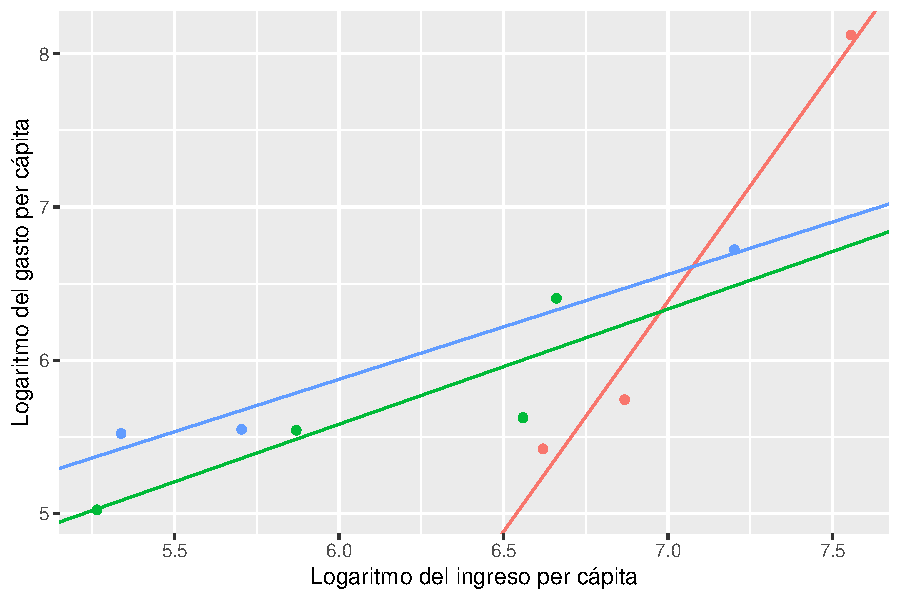
\includegraphics[width=0.7\linewidth,height=\textheight,keepaspectratio]{chapters/../figures/fig-intercept-slope-free-1.pdf}

}

\caption{\label{fig-intercept-slope-free}Modelo con intercepto y
pendiente específicos por estrato (ajuste independiente)}

\end{figure}%

Al estimar ambos coeficientes por separado para cada estrato, las
elasticidades van de 0,684 a 3,008, según la
tabla~\ref{tbl-motivation-models}. En el estrato idStrt039, un ingreso 1
\% mayor se asocia con un gasto aproximadamente 3,008 \% mayor,
manteniendo constantes las demás variables incluidas en el modelo. Estas
estimaciones corresponden a ajustes independientes en grupos pequeños y
no incorporan todavía el control por edad.

Aunque esta última especificación ofrece una representación más flexible
de los datos y permite capturar las particularidades de cada estrato,
presenta una limitación importante: los parámetros se estiman de manera
completamente independiente para cada grupo. Como consecuencia, no se
aprovecha la información compartida entre estratos que podrían presentar
patrones similares, lo que puede generar estimaciones inestables,
especialmente en aquellos grupos con un número reducido de
observaciones. Los modelos multinivel superan esta dificultad mediante
un mecanismo conocido como encogimiento (\emph{shrinkage}), en el cual
las estimaciones específicas de cada grupo se obtienen combinando la
información propia del grupo con la información proveniente del conjunto
de la población (\citeproc{ref-gelman2006data}{Gelman y Hill 2006};
\citeproc{ref-goldstein2011multilevel}{Goldstein 2011}). De esta manera,
se logra un equilibrio entre la representación de las diferencias entre
estratos y la eficiencia estadística de las estimaciones.

La tabla~\ref{tbl-motivation-models} reúne los coeficientes de los
cuatro ajustes en el orden en que se han presentado. Como el ingreso y
el gasto están en logaritmos, la pendiente es también la elasticidad y
se muestra en una sola columna. El intercepto no tiene esa
interpretación. El siguiente código computacional combina los
coeficientes guardados durante los ajustes para facilitar su
comparación.

\begin{Shaded}
\begin{Highlighting}[]
\NormalTok{motivation\_models\_table }\OtherTok{\textless{}{-}} \FunctionTok{bind\_rows}\NormalTok{(}
  \StringTok{"Regresión simple"} \OtherTok{=} \FunctionTok{tibble}\NormalTok{(}
    \AttributeTok{Stratum =} \StringTok{"Tres estratos juntos"}\NormalTok{,}
    \AttributeTok{beta\_0 =} \FunctionTok{unname}\NormalTok{(}\FunctionTok{coef}\NormalTok{(simple\_model)[}\DecValTok{1}\NormalTok{]),}
    \AttributeTok{beta\_1 =} \FunctionTok{unname}\NormalTok{(}\FunctionTok{coef}\NormalTok{(simple\_model)[}\DecValTok{2}\NormalTok{])}
\NormalTok{  ),}
  \StringTok{"Interceptos específicos y pendiente común"} \OtherTok{=}\NormalTok{ common\_slope\_coefficients,}
  \StringTok{"Intercepto común y pendientes específicas"} \OtherTok{=}\NormalTok{ common\_intercept\_coefficients,}
  \StringTok{"Interceptos y pendientes específicos"} \OtherTok{=}\NormalTok{ separate\_coefficients,}
  \AttributeTok{.id =} \StringTok{"model"}
\NormalTok{) }\SpecialCharTok{\%\textgreater{}\%}
  \FunctionTok{select}\NormalTok{(model, Stratum, beta\_0, beta\_1)}

\NormalTok{motivation\_models\_table}
\end{Highlighting}
\end{Shaded}

{

\begin{longtable}[]{@{}
  >{\raggedright\arraybackslash}p{(\linewidth - 6\tabcolsep) * \real{0.4286}}
  >{\raggedright\arraybackslash}p{(\linewidth - 6\tabcolsep) * \real{0.2143}}
  >{\raggedleft\arraybackslash}p{(\linewidth - 6\tabcolsep) * \real{0.1122}}
  >{\raggedleft\arraybackslash}p{(\linewidth - 6\tabcolsep) * \real{0.2449}}@{}}

\caption{\label{tbl-motivation-models}Interceptos y elasticidades de los
modelos ilustrativos de la sección de motivación}

\tabularnewline

\toprule\noalign{}
\begin{minipage}[b]{\linewidth}\raggedright
Modelo
\end{minipage} & \begin{minipage}[b]{\linewidth}\raggedright
Estrato
\end{minipage} & \begin{minipage}[b]{\linewidth}\raggedleft
Intercepto
\end{minipage} & \begin{minipage}[b]{\linewidth}\raggedleft
Pendiente (elasticidad)
\end{minipage} \\
\midrule\noalign{}
\endhead
\bottomrule\noalign{}
\endlastfoot
Regresión simple & Tres estratos juntos & 0.205 & 0.906 \\
Interceptos específicos y pendiente común & idStrt039 & 0.077 & 0.906 \\
Interceptos específicos y pendiente común & idStrt046 & 0.135 & 0.906 \\
Interceptos específicos y pendiente común & idStrt057 & 0.424 & 0.906 \\
Intercepto común y pendientes específicas & idStrt039 & 0.205 & 0.894 \\
Intercepto común y pendientes específicas & idStrt046 & 0.205 & 0.893 \\
Intercepto común y pendientes específicas & idStrt057 & 0.205 & 0.937 \\
Interceptos y pendientes específicos & idStrt039 & -14.669 & 3.008 \\
Interceptos y pendientes específicos & idStrt046 & 1.073 & 0.752 \\
Interceptos y pendientes específicos & idStrt057 & 1.770 & 0.684 \\

\end{longtable}

}

\section{Incorporación de pesos de muestreo en modelos
multinivel}\label{pesos-q-weighted}

En el contexto de los modelos multinivel con datos provenientes de
encuestas, una dificultad adicional radica en la incorporación coherente
de los pesos de muestreo a través de los distintos niveles de la
jerarquía. La estructura agrupada de los datos implica que las
observaciones no son independientes, por lo que la función de
log-verosimilitud no puede descomponerse como una suma simple de
contribuciones individuales. En su lugar, es necesario considerar
explícitamente la dependencia entre los distintos niveles del diseño
muestral para lograr inferencias adecuadas.

La incorporación de los pesos de muestreo en modelos multinivel ha
recibido una atención considerable en la literatura, especialmente
cuando el diseño de la encuesta puede ser informativo. En estos casos,
la probabilidad de inclusión de las unidades puede estar relacionada con
las variables de interés, incluso después de condicionar por las
covariables incluidas en el modelo. Ignorar esta característica del
diseño puede afectar la estimación de los parámetros y, en consecuencia,
la validez de las inferencias obtenidas a partir del modelo
(\citeproc{ref-pfeffermann1998weighting}{Pfeffermann et~al. 1998};
\citeproc{ref-asparouhov2006general}{Asparouhov 2006}).

Una de las principales alternativas consiste en extender los métodos de
estimación habituales mediante procedimientos de pseudo-máxima
verosimilitud, incorporando los pesos de muestreo en la función objetivo
utilizada para estimar los parámetros. Como se ha mencionado a lo largo
de este documento, dentro de este enfoque se han propuesto diferentes
formas de ponderar las contribuciones de las unidades y de los
conglomerados a la función de verosimilitud
(\citeproc{ref-rabehesketh2006multilevel}{Rabe-Hesketh y Skrondal 2006};
\citeproc{ref-Carle2009}{Carle 2009}). Estas estrategias buscan
preservar, en la medida de lo posible, las ventajas de la modelación
jerárquica al tiempo que incorporan información procedente del diseño
muestral.

También se han desarrollado procedimientos de estimación basados en
algoritmos iterativos, incluidos enfoques que utilizan variantes del
algoritmo EM para incorporar las ponderaciones dentro de la estimación
de modelos jerárquicos (\citeproc{ref-cai2013investigation}{Cai 2013}).
En conjunto, estos trabajos muestran que no existe una única manera de
incorporar los pesos de muestreo en modelos multinivel. La elección del
procedimiento depende, entre otros factores, de la estructura del diseño
muestral, del nivel o los niveles en los que se produce la selección
informativa y del objetivo inferencial del análisis. Por esta razón, más
que considerar la ponderación como una corrección mecánica, resulta
conveniente evaluar explícitamente las características del diseño y el
posible carácter informativo del mecanismo de selección antes de definir
la estrategia de estimación.

Como explica Pfeffermann
(\citeproc{ref-pfeffermann2011modelling}{2011}), para ajustar modelos
multinivel con datos provenientes de encuestas complejas, una
alternativa consiste en utilizar el enfoque de pesos \emph{q-weighted}.
La idea central de este método es eliminar de los pesos muestrales la
componente sistemática explicada por las covariables incluidas en el
modelo, de modo que los pesos resultantes conserven únicamente la parte
residual atribuible al mecanismo de selección.

No obstante, este no es el único enfoque disponible para la estimación
de modelos multinivel con datos de encuestas complejas y tampoco
sustituye el uso de pesos condicionales o de pesos escalados en cada
etapa del diseño, requeridos por algunos métodos de pseudo-verosimilitud
multinivel. El procedimiento para construir los pesos \emph{q-weighted}
se resume en los siguientes pasos:

\begin{enumerate}
\def\labelenumi{\arabic{enumi}.}
\item
  Ajustar un modelo de regresión para los factores de expansión finales
  de la encuesta, utilizando como variables explicativas el mismo
  conjunto de covariables que será empleado en el modelo multinivel.
  Siendo \(w_k\) el factor de expansión original de la unidad \(k\) y
  \(\mathbf{x}_k\) el vector de covariables. Entonces se ajusta el
  modelo

  \[
  w_k = f(\mathbf{x}_k, \boldsymbol{\beta}) + \varepsilon_k,
  \]

  donde \(f(\cdot)\) representa la relación funcional entre los pesos
  \(w_k\) y las covariables \(\mathbf{x}_k\), a través de los
  coeficientes \(\boldsymbol{\beta}\).
\item
  Obtener los valores predichos del modelo para cada unidad de
  observación, de tal forma que:

  \[
  \hat{w}_k = f(\mathbf{x}_k, \hat{\boldsymbol{\beta}}).
  \]

  Estos valores representan la componente de los factores de expansión
  explicada por las covariables incluidas en el modelo.
\item
  Construir los pesos \emph{q-weighted} dividiendo los factores de
  expansión originales por la estimación de su esperanza condicional en
  la muestra,

  \begin{equation}\protect\phantomsection\label{eq-pesos-q}{
  q_k = \frac{w_k}{\widehat{E}_s(w_k\mid\mathbf{x}_k)}.
  }\end{equation}

  De esta forma, los nuevos pesos reflejan la variación residual de los
  factores de expansión una vez controlado el efecto de las covariables.
\item
  En la implementación ilustrativa de este capítulo, pasar los pesos
  ajustados \(q_k\) al argumento \texttt{weights} de \texttt{lmer()} y
  \texttt{glmer()}. Este paso no construye un objeto de diseño muestral
  ni incorpora por sí solo los pesos de selección por etapa o la
  estimación de varianza bajo el diseño complejo.
\end{enumerate}

El siguiente código implementa el procedimiento de construcción de pesos
\emph{q-weighted} y fija \texttt{reference\_age} en la mediana de la
edad para representar los modelos lineales a una edad común. En primer
lugar, ajusta un modelo de regresión lineal que explica los factores de
expansión originales a partir del logaritmo del ingreso y la edad de la
persona principal. De esta forma, los pesos resultantes conservan
únicamente la componente de variación no explicada por las covariables
incluidas en el modelo multinivel.

\begin{Shaded}
\begin{Highlighting}[]
\NormalTok{mod\_qw }\OtherTok{\textless{}{-}} \FunctionTok{lm}\NormalTok{(wk }\SpecialCharTok{\textasciitilde{}}\NormalTok{ log\_income }\SpecialCharTok{+}\NormalTok{ Age, }\AttributeTok{data =}\NormalTok{ survey\_data)}
\NormalTok{predicted\_weights }\OtherTok{\textless{}{-}} \FunctionTok{predict}\NormalTok{(mod\_qw)}
\NormalTok{survey\_data}\SpecialCharTok{$}\NormalTok{qk }\OtherTok{\textless{}{-}}\NormalTok{ survey\_data}\SpecialCharTok{$}\NormalTok{wk }\SpecialCharTok{/}\NormalTok{ predicted\_weights}
\NormalTok{reference\_age }\OtherTok{\textless{}{-}} \FunctionTok{median}\NormalTok{(survey\_data}\SpecialCharTok{$}\NormalTok{Age)}
\end{Highlighting}
\end{Shaded}

El ajuste lineal de los factores de expansión según el logaritmo del
ingreso y la edad constituye una aproximación para construir los pesos
\emph{q-weighted}. Para construir estos pesos, las predicciones deben
ser finitas y estrictamente positivas. También debe evaluarse si el
modelo representa adecuadamente \(E_s(w_k\mid\mathbf{x}_k)\), pues una
regresión lineal de los pesos puede producir predicciones no válidas.
Además, el vector \texttt{qk} no necesariamente permite reconstruir por
sí solo los pesos condicionales de cada etapa que requiere un modelo
multinivel ponderado.

Para representar los modelos lineales de la siguiente sección, se
utiliza \texttt{reference\_age} como una edad común de la persona
principal del hogar. Su valor se obtiene con
\texttt{median(survey\_data\$Age)} y corresponde a 47 años. Al mantener
fija la edad en las rectas de regresión, las comparaciones entre
estratos describen la relación entre ingreso y gasto sin incorporar
diferencias de edad entre los hogares representados. Esta referencia se
aplica únicamente a la visualización: los modelos se estiman utilizando
las edades observadas de todos los hogares.

\section{Modelo lineal multinivel}\label{modelo-lineal-multinivel}

Los modelos multinivel más utilizados en la práctica corresponden a
extensiones del modelo lineal clásico para datos con estructura
jerárquica. En su formulación básica, estos modelos asumen que la
variable respuesta es continua y sigue una distribución normal
condicional a los efectos fijos y aleatorios incluidos en el modelo.
Asimismo, se supone que los efectos aleatorios y los errores residuales
son independientes entre sí y se distribuyen normalmente con media cero
y varianzas constantes.

En esta sección se modela el logaritmo del gasto mensual per cápita del
hogar, representado por \(y_{kj}\), donde \(k\) identifica al hogar y
\(j\) al estrato. Los modelos con covariables incorporan el logaritmo
del ingreso per cápita, representado por \(x_{kj}\), y la edad de la
persona principal como control. Por ello, las predicciones se obtienen
inicialmente en la escala logarítmica. Al aplicarles la función
exponencial, se regresa a las unidades monetarias del gasto, pero el
resultado representa una media geométrica: una medida del gasto típico
para hogares con esas características y ese efecto de estrato. Para
estimar el gasto medio aritmético se requiere, además, considerar la
variabilidad residual del modelo.

\subsection{Modelo nulo}\label{sec-multinivel-muestras-complejas}

En el análisis de regresión multinivel, se distinguen dos tipos de
parámetros: los coeficientes de regresión, conocidos como parámetros
fijos, y los componentes de varianza asociados a los efectos aleatorios
(\citeproc{ref-goldstein2011multilevel}{Goldstein 2011};
\citeproc{ref-rabehesketh2012multilevel}{Rabe-Hesketh y Skrondal 2012},
e). Una etapa inicial fundamental en este tipo de análisis consiste en
descomponer la variabilidad total de la variable dependiente en los
distintos niveles de la estructura jerárquica. En el contexto del
ejemplo anterior, esta descomposición permite separar la variación del
logaritmo del gasto en una componente atribuible a diferencias dentro de
los estratos y otra asociada a diferencias entre estratos.

Según Snijders y Bosker (\citeproc{ref-snijders2011}{2011}), el punto de
partida para esta descomposición es el denominado modelo nulo, el cual
no incorpora variables explicativas y se expresa como

\begin{equation}\protect\phantomsection\label{eq-modelo-multinivel-nulo}{
y_{kj} = \beta_{0j} + \epsilon_{kj}
}\end{equation}

En donde \(y_{kj}\) denota el valor observado del logaritmo del gasto
para la unidad \(k\) en el estrato \(j\). El término \(\beta_{0j}\)
representa el intercepto específico de cada estrato, capturando las
diferencias en los niveles promedio de la variable entre grupos.
Finalmente, \(\epsilon_{kj}\) corresponde al error a nivel de unidad, el
cual recoge la variabilidad no explicada dentro de cada estrato y se
asume con media cero y varianza constante condicional al grupo.

A su vez, el intercepto por estrato puede descomponerse en una parte
común a todos los estratos y una desviación específica de cada uno de
ellos, de la siguiente forma:

\[
\beta_{0j} = \gamma_{00} + \tau_{0j}
\]

donde \(\gamma_{00}\) representa el intercepto promedio global y
\(\tau_{0j}\) es el efecto aleatorio para el intercepto que captura la
desviación del estrato \(j\), permitiendo modelar explícitamente la
heterogeneidad entre estratos. Además, los componentes aleatorios del
modelo se asumen distribuidos normalmente con media cero y varianzas
específicas para cada nivel de la jerarquía. En particular, el efecto
aleatorio asociado al intercepto por estrato cumple

\[
\tau_{0j} \sim N\left(0, \sigma_{\tau}^{2}\right),
\]

lo que implica que las desviaciones de cada estrato respecto al
intercepto global se distribuyen alrededor de cero, con una variabilidad
determinada por \(\sigma_{\tau}^{2}\). De manera análoga, el término de
error a nivel de unidad sigue la distribución

\[
\epsilon_{kj} \sim N\left(0, \sigma_{\epsilon}^{2}\right),
\]

Donde \(\sigma_{\epsilon}^{2}\) representa la variabilidad residual
dentro de los estratos. A partir de este modelo se define el coeficiente
de correlación intraclase (ICC, por sus siglas en inglés), que
cuantifica la proporción de la varianza total explicada por las
diferencias entre estratos. Su definición se presenta a continuación:

\begin{equation}\protect\phantomsection\label{eq-cci-lineal}{
\rho = \frac{\sigma_{\tau}^{2}}{\sigma_{\tau}^{2} + \sigma_{\epsilon}^{2}}
}\end{equation}

De acuerdo con Bates et~al. (\citeproc{ref-BatesEtAl2015}{2015}), un
valor elevado de ICC indica que una proporción importante de la
variabilidad total de la variable de interés se debe a diferencias entre
estratos, lo que sugiere la presencia de heterogeneidad relevante entre
grupos y la necesidad de incorporar explícitamente dicha estructura en
el modelo. En contraste, un ICC bajo implica que la variabilidad se
concentra principalmente dentro de los estratos, los cuales presentan
una mayor homogeneidad relativa entre sí.

Siguiendo con el análisis de la encuesta de ejemplo, cuando la variable
de interés es el logaritmo del gasto, el modelo nulo constituye el punto
de partida para cuantificar qué proporción de la variabilidad total se
debe a diferencias entre estratos y qué proporción corresponde a
diferencias entre hogares dentro de un mismo estrato.

La estimación de modelos multinivel en \texttt{R} se realiza mediante el
paquete \texttt{lme4}. En particular, la función \texttt{lmer()} permite
especificar los efectos aleatorios mediante expresiones de la forma
\texttt{(efecto\ \textbar{}\ grupo)}. En este contexto, la expresión
\texttt{(1\ \textbar{}\ Stratum)} indica que el modelo incluye un
intercepto aleatorio para cada estrato. El valor \texttt{1} representa
el intercepto del modelo, mientras que \texttt{Stratum} identifica la
variable de agrupación.

Como advierte Carle (\citeproc{ref-Carle2009}{2009}), en \texttt{lme4},
el argumento \texttt{weights} representa pesos previos que modifican la
contribución residual, pero no implementa por sí solo la
pseudo-verosimilitud multinivel con pesos de diseño por etapa ni la
estimación de varianza del diseño. Por tanto, los modelos ponderados con
\texttt{qk} que siguen deben interpretarse como una ilustración
modelada, no como una solución general para inferencia de encuestas
complejas; para ese propósito se requieren pesos escalados y software
que los incorpore expresamente en la estimación multinivel. El siguiente
código computacional ajusta el modelo nulo con intercepto aleatorio por
estrato.

\begin{Shaded}
\begin{Highlighting}[]
\NormalTok{mod\_null }\OtherTok{\textless{}{-}} \FunctionTok{lmer}\NormalTok{(}
\NormalTok{  log\_expenditure }\SpecialCharTok{\textasciitilde{}}\NormalTok{ (}\DecValTok{1} \SpecialCharTok{|}\NormalTok{ Stratum),}
  \AttributeTok{data =}\NormalTok{ survey\_data,}
  \AttributeTok{weights =}\NormalTok{ qk}
\NormalTok{)}
\end{Highlighting}
\end{Shaded}

Las tablas de coeficientes por estrato presentan las estimaciones
condicionales del modelo. Cada fila identifica el estrato y el parámetro
correspondiente. Los estadísticos de prueba y los valores-\emph{p} de
los efectos fijos corresponden a otro nivel de inferencia. El siguiente
código computacional extrae los interceptos estimados por estrato y los
organiza para su presentación.

\begin{Shaded}
\begin{Highlighting}[]
\NormalTok{coef\_mod\_null }\OtherTok{\textless{}{-}} \FunctionTok{coef}\NormalTok{(mod\_null)}\SpecialCharTok{$}\NormalTok{Stratum}
\NormalTok{null\_model\_intercepts\_table }\OtherTok{\textless{}{-}}\NormalTok{ coef\_mod\_null }\SpecialCharTok{\%\textgreater{}\%}
\NormalTok{  tibble}\SpecialCharTok{::}\FunctionTok{rownames\_to\_column}\NormalTok{(}\StringTok{"stratum"}\NormalTok{) }\SpecialCharTok{\%\textgreater{}\%}
  \FunctionTok{slice}\NormalTok{(}\DecValTok{1}\SpecialCharTok{:}\DecValTok{5}\NormalTok{L) }\SpecialCharTok{\%\textgreater{}\%}
  \FunctionTok{transmute}\NormalTok{(stratum, }\AttributeTok{intercept =}\NormalTok{ .data[[}\StringTok{"(Intercept)"}\NormalTok{]])}

\NormalTok{null\_model\_intercepts\_table}
\end{Highlighting}
\end{Shaded}

{

\begin{longtable}[]{@{}lr@{}}

\caption{\label{tbl-interceptos-nulos}Interceptos estimados por estrato
bajo pesos q-weighted (modelo nulo, primeros 5 estratos)}

\tabularnewline

\toprule\noalign{}
Estrato & Intercepto (beta) \\
\midrule\noalign{}
\endhead
\bottomrule\noalign{}
\endlastfoot
idStrt001 & 5.53 \\
idStrt002 & 5.57 \\
idStrt003 & 5.55 \\
idStrt004 & 5.97 \\
idStrt005 & 5.91 \\

\end{longtable}

}

La tabla~\ref{tbl-interceptos-nulos} presenta los interceptos estimados
para los primeros 5 estratos a partir del modelo nulo. Por ejemplo, el
intercepto del estrato idStrt001 es 5,527 y representa el valor esperado
del logaritmo del gasto mensual per cápita en ese estrato. Como este
modelo no incluye el ingreso ni otras covariables, no estima
elasticidades. Su función es describir la variación del logaritmo del
gasto entre estratos antes de incorporar los predictores.

El siguiente código computacional calcula la correlación intraclase a
partir de los componentes de varianza del modelo nulo mediante
\texttt{icc()} del paquete \texttt{performance}
(\citeproc{ref-performance2026}{Lüdecke et~al. 2026}). Este indicador
cuantifica la proporción de la variabilidad total del logaritmo del
gasto que puede atribuirse a diferencias entre estratos, constituyendo
una medida de la dependencia existente entre observaciones
pertenecientes a un mismo grupo. Los resultados obtenidos se presentan
en la tabla~\ref{tbl-icc-nulo}.

\begin{Shaded}
\begin{Highlighting}[]
\NormalTok{null\_model\_icc\_table }\OtherTok{\textless{}{-}}\NormalTok{ performance}\SpecialCharTok{::}\FunctionTok{icc}\NormalTok{(mod\_null) }\SpecialCharTok{\%\textgreater{}\%}
  \FunctionTok{as.data.frame}\NormalTok{()}

\NormalTok{null\_model\_icc\_table}
\end{Highlighting}
\end{Shaded}

{

\begin{longtable}[]{@{}rrl@{}}

\caption{\label{tbl-icc-nulo}Correlación intraclase del modelo nulo
(logaritmo del gasto por estrato)}

\tabularnewline

\toprule\noalign{}
CCI ajustado & CCI sin ajustar & Opcional \\
\midrule\noalign{}
\endhead
\bottomrule\noalign{}
\endlastfoot
0.203 & 0.203 & FALSE \\

\end{longtable}

}

La correlación intraclase estimada es de 0,203. Bajo esta descomposición
del modelo, aproximadamente el 20 \% de la variabilidad se atribuye al
componente entre estratos. El modelo nulo no incluye predictores, por lo
que el valor esperado del logaritmo del gasto per cápita es constante
dentro de cada estrato e igual a su intercepto estimado.

\subsection{Modelo con intercepto
aleatorio}\label{sec-intercepto-aleatorio}

De acuerdo con Goldstein (\citeproc{ref-goldstein2011multilevel}{2011})
y Rabe-Hesketh y Skrondal
(\citeproc{ref-rabehesketh2012multilevel}{2012}), el modelo multinivel
más simple que incorpora covariables corresponde al modelo de intercepto
aleatorio. En esta especificación, se asume que los efectos de las
variables explicativas son comunes a todos los estratos, mientras que el
nivel promedio de la variable respuesta puede variar entre ellos. El
modelo se expresa como

\begin{equation}\protect\phantomsection\label{eq-modelo-intercepto-aleatorio}{
y_{kj} = \beta_{0j} + \mathbf{x}_{kj}\boldsymbol{\beta} + \epsilon_{kj}
}\end{equation}

En donde \(y_{kj}\) representa el valor observado de la variable
respuesta para la unidad \(k\) perteneciente al estrato \(j\),
\(\mathbf{x}_{kj}\) es el vector de covariables asociado a dicha unidad,
\(\boldsymbol{\beta}\) es el vector de coeficientes de regresión comunes
a todos los estratos y \(\epsilon_{kj}\) corresponde al error aleatorio
a nivel de unidad.

Al igual que en el modelo nulo, el intercepto se modela como
\(\beta_{0j} = \gamma_{00} + \tau_{0j}\); en donde \(\gamma_{00}\)
representa el intercepto promedio global y \(\tau_{0j}\) es el efecto
aleatorio asociado al estrato \(j\), que mide la desviación de dicho
estrato respecto al promedio general.

Los componentes aleatorios del modelo se asumen independientes y
normalmente distribuidos, de manera que
\(\tau_{0j} \sim N(0,\sigma_{\tau}^{2})\) y
\(\epsilon_{kj} \sim N(0,\sigma_{\epsilon}^{2})\). Bajo estas
condiciones, la variabilidad total de la variable respuesta puede
descomponerse en una componente entre estratos, cuantificada por
\(\sigma_{\tau}^{2}\), y una componente dentro de los estratos,
representada por \(\sigma_{\epsilon}^{2}\).

El siguiente código ajusta un modelo multinivel de intercepto aleatorio,
en donde el logaritmo del gasto per cápita (\texttt{log\_expenditure})
se explica a partir del logaritmo del ingreso per cápita
(\texttt{log\_income}), controlando por la edad (\texttt{Age}) como
efecto fijo común e incorporando además un efecto aleatorio asociado al
estrato (\texttt{Stratum}) y utilizando los pesos \emph{q-weighted}
almacenados en la variable \texttt{qk}. Una vez ajustado el modelo, se
estima la correlación intraclase (ICC) a partir de los componentes de
varianza estimados.

\begin{Shaded}
\begin{Highlighting}[]
\NormalTok{random\_intercept\_model }\OtherTok{\textless{}{-}} \FunctionTok{lmer}\NormalTok{(}
\NormalTok{  log\_expenditure }\SpecialCharTok{\textasciitilde{}}\NormalTok{ log\_income }\SpecialCharTok{+}\NormalTok{ Age }\SpecialCharTok{+}\NormalTok{ (}\DecValTok{1} \SpecialCharTok{|}\NormalTok{ Stratum),}
  \AttributeTok{data =}\NormalTok{ survey\_data,}
  \AttributeTok{weights =}\NormalTok{ qk}
\NormalTok{)}

\NormalTok{random\_intercept\_model\_icc }\OtherTok{\textless{}{-}}\NormalTok{ performance}\SpecialCharTok{::}\FunctionTok{icc}\NormalTok{(random\_intercept\_model)}
\NormalTok{random\_intercept\_model\_icc}
\end{Highlighting}
\end{Shaded}

Una vez controlados el logaritmo del ingreso per cápita y la edad, el
ICC ajustado es 0,075. Esto indica que alrededor del 7,5 \% de la
variabilidad residual corresponde a diferencias entre estratos; el resto
se observa entre hogares del mismo estrato. El valor es menor que en el
modelo nulo, que no incluye covariables. Sin embargo, el ICC por sí solo
no determina si conviene usar un modelo multinivel: también importa si
los estratos son grupos adecuados para el análisis y qué muestran los
diagnósticos del modelo. Los coeficientes estimados por estrato se
presentan en la tabla~\ref{tbl-coef-intercepto-aleatorio}.

La elasticidad común estimada del gasto respecto al ingreso es 0,559.
Dentro de un mismo estrato y manteniendo constante la edad de la persona
principal, un aumento del 1 \% en el ingreso per cápita se asocia con un
aumento aproximado del 0,559 \% en el gasto per cápita típico, expresado
mediante su media geométrica condicional. Para un aumento del 10 \% en
el ingreso, el cambio se calcula como \(100[(1+0,10)^{\hat{\beta}}-1]\),
donde \(\hat{\beta}\) es la elasticidad estimada. En este modelo, el
resultado es 5,47 \%. Esta interpretación describe una asociación, sin
establecer causalidad. Los interceptos corresponden a un ingreso de una
unidad monetaria y una edad de cero años; estos valores están fuera del
rango observado, por lo que no deben interpretarse como el gasto
habitual de los hogares.

El coeficiente de la edad es una semielasticidad y su estimación es
-0,0017. Para iguales ingreso per cápita y estrato, un año adicional de
edad se asocia con un cambio del -0,17 \% en la media geométrica
condicional del gasto. El signo negativo describe una asociación
ajustada, sin implicar causalidad. El siguiente código computacional
presenta en columnas separadas el intercepto, la elasticidad del ingreso
y el coeficiente de edad para cada estrato.

\begin{Shaded}
\begin{Highlighting}[]
\NormalTok{random\_intercept\_coefficients\_table }\OtherTok{\textless{}{-}} \FunctionTok{coef}\NormalTok{(random\_intercept\_model)}\SpecialCharTok{$}\NormalTok{Stratum }\SpecialCharTok{\%\textgreater{}\%}
\NormalTok{  tibble}\SpecialCharTok{::}\FunctionTok{rownames\_to\_column}\NormalTok{(}\StringTok{"stratum"}\NormalTok{) }\SpecialCharTok{\%\textgreater{}\%}
  \FunctionTok{slice}\NormalTok{(}\DecValTok{1}\SpecialCharTok{:}\DecValTok{5}\NormalTok{L) }\SpecialCharTok{\%\textgreater{}\%}
  \FunctionTok{transmute}\NormalTok{(}
\NormalTok{    stratum,}
    \AttributeTok{intercept =}\NormalTok{ .data[[}\StringTok{"(Intercept)"}\NormalTok{]],}
    \AttributeTok{income\_elasticity =}\NormalTok{ log\_income,}
    \AttributeTok{age\_coefficient =}\NormalTok{ Age}
\NormalTok{  )}

\NormalTok{random\_intercept\_coefficients\_table}
\end{Highlighting}
\end{Shaded}

{

\begin{longtable}[]{@{}lrrr@{}}

\caption{\label{tbl-coef-intercepto-aleatorio}Interceptos, elasticidad
del ingreso y coeficiente de edad por estrato (5 estratos)}

\tabularnewline

\toprule\noalign{}
Estrato & Intercepto & Elasticidad del ingreso & Coeficiente de edad \\
\midrule\noalign{}
\endhead
\bottomrule\noalign{}
\endlastfoot
idStrt001 & 2.34 & 0.559 & -0.002 \\
idStrt002 & 2.34 & 0.559 & -0.002 \\
idStrt003 & 2.33 & 0.559 & -0.002 \\
idStrt004 & 2.40 & 0.559 & -0.002 \\
idStrt005 & 2.49 & 0.559 & -0.002 \\

\end{longtable}

}

En la tabla~\ref{tbl-coef-intercepto-aleatorio}, el coeficiente de
\texttt{log\_income} se repite en los cinco estratos porque la
elasticidad es común. Las diferencias de intercepto desplazan las
rectas, pero no modifican la respuesta proporcional del gasto ante un
cambio porcentual en el ingreso. Los interceptos no son elasticidades y
el coeficiente de \texttt{Age} es una semielasticidad, dado que la edad
se incorpora en años.

Para visualizar los resultados a una edad común en la submuestra de tres
estratos definida anteriormente, el siguiente código computacional
selecciona los coeficientes correspondientes del modelo ajustado.

\begin{Shaded}
\begin{Highlighting}[]
\NormalTok{estimated\_coef }\OtherTok{\textless{}{-}} \FunctionTok{inner\_join}\NormalTok{(}
  \FunctionTok{coef}\NormalTok{(random\_intercept\_model)}\SpecialCharTok{$}\NormalTok{Stratum }\SpecialCharTok{\%\textgreater{}\%}
\NormalTok{    tibble}\SpecialCharTok{::}\FunctionTok{rownames\_to\_column}\NormalTok{(}\AttributeTok{var =} \StringTok{"Stratum"}\NormalTok{),}
\NormalTok{  plot\_data }\SpecialCharTok{\%\textgreater{}\%}
    \FunctionTok{select}\NormalTok{(Stratum) }\SpecialCharTok{\%\textgreater{}\%}
    \FunctionTok{distinct}\NormalTok{()}
\NormalTok{)}
\end{Highlighting}
\end{Shaded}

Las rectas se representan para una persona principal de 47 años, sumando
al intercepto el producto del coeficiente de \texttt{Age} por
\texttt{reference\_age}. Los puntos muestran los datos observados de
hogares con distintas edades, por lo que no son observaciones ajustadas
a esa edad común. La figura~\ref{fig-intercept-random}, obtenida con el
siguiente código computacional, muestra las rectas de regresión
estimadas para cada estrato bajo el modelo de intercepto aleatorio. Se
observa que las rectas comparten una misma pendiente, reflejando la
asociación común entre el logaritmo del ingreso y el del gasto, pero
difieren en su posición vertical debido a los interceptos específicos
estimados para cada estrato.

\begin{Shaded}
\begin{Highlighting}[]
\FunctionTok{ggplot}\NormalTok{(}
  \AttributeTok{data =}\NormalTok{ plot\_data,}
  \FunctionTok{aes}\NormalTok{(}
    \AttributeTok{y =}\NormalTok{ log\_expenditure,}
    \AttributeTok{x =}\NormalTok{ log\_income,}
    \AttributeTok{colour =}\NormalTok{ Stratum}
\NormalTok{  )}
\NormalTok{) }\SpecialCharTok{+}
  \FunctionTok{geom\_point}\NormalTok{() }\SpecialCharTok{+}
  \FunctionTok{labs}\NormalTok{(}\AttributeTok{x =} \StringTok{"Logaritmo del ingreso per cápita"}\NormalTok{,}
       \AttributeTok{y =} \StringTok{"Logaritmo del gasto per cápita"}\NormalTok{) }\SpecialCharTok{+}
  \FunctionTok{geom\_abline}\NormalTok{(}
    \AttributeTok{data =}\NormalTok{ estimated\_coef,}
    \AttributeTok{mapping =} \FunctionTok{aes}\NormalTok{(}
      \AttributeTok{slope =}\NormalTok{ log\_income,}
      \AttributeTok{intercept =} \StringTok{\textasciigrave{}}\AttributeTok{(Intercept)}\StringTok{\textasciigrave{}} \SpecialCharTok{+}\NormalTok{ Age }\SpecialCharTok{*}\NormalTok{ reference\_age,}
      \AttributeTok{colour =}\NormalTok{ Stratum}
\NormalTok{    )}
\NormalTok{  ) }\SpecialCharTok{+}
  \FunctionTok{theme}\NormalTok{(}
    \AttributeTok{legend.position =} \StringTok{"none"}\NormalTok{,}
    \AttributeTok{plot.title =} \FunctionTok{element\_text}\NormalTok{(}\AttributeTok{hjust =} \FloatTok{0.5}\NormalTok{)}
\NormalTok{  )}
\end{Highlighting}
\end{Shaded}

\begin{figure}[H]

\centering{

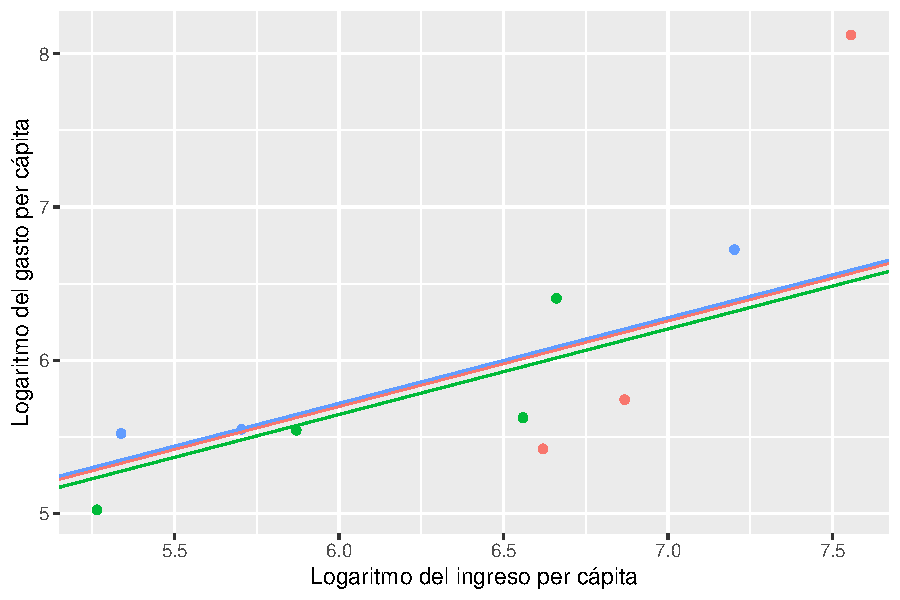
\includegraphics[width=0.7\linewidth,height=\textheight,keepaspectratio]{chapters/../figures/fig-intercept-random-1.pdf}

}

\caption{\label{fig-intercept-random}Rectas de regresión estimadas por
estrato: modelo con intercepto aleatorio}

\end{figure}%

\subsection{Modelo con intercepto y pendiente
aleatoria}\label{sec-intercepto-pendiente-aleatorios}

De acuerdo con Goldstein (\citeproc{ref-goldstein2011multilevel}{2011})
y Snijders y Bosker (\citeproc{ref-snijders2011}{2011}), una extensión
natural del modelo anterior es el modelo de intercepto y pendiente
aleatorios. En esta especificación, no sólo se permite que el nivel
promedio de la variable respuesta varíe entre estratos, sino también que
el efecto de una o más covariables difiera entre grupos. De esta manera,
cada estrato puede tener su propia recta de regresión, tanto en términos
de intercepto como de pendiente. El modelo puede expresarse como

\begin{equation}\protect\phantomsection\label{eq-modelo-pendiente-aleatoria}{
y_{kj} = \beta_{0j} + x_{kj}\beta_{1j} + \mathbf{z}_{kj}\boldsymbol{\beta} + \epsilon_{kj},
}\end{equation}

donde \(y_{kj}\) representa el valor observado de la variable respuesta
para la unidad \(k\) perteneciente al estrato \(j\), \(x_{kj}\)
corresponde a la covariable cuya pendiente se permite variar entre
estratos, \(\mathbf{z}_{kj}\) contiene las covariables con efectos fijos
comunes a todos los grupos, y \(\epsilon_{kj}\) es el término de error a
nivel de unidad. En este modelo, tanto el intercepto como la pendiente
asociada a \(x_{kj}\) se consideran aleatorios y se descomponen de la
siguiente forma:

\[
\beta_{0j} = \gamma_{00} + \tau_{0j}, \qquad
\beta_{1j} = \gamma_{10} + \tau_{1j}
\]

donde \(\gamma_{00}\) y \(\gamma_{10}\) representan, respectivamente, el
intercepto y la pendiente promedio en la población, mientras que
\(\tau_{0j}\) y \(\tau_{1j}\) capturan las desviaciones específicas del
estrato \(j\) respecto a dichos promedios. Estos efectos aleatorios se
asumen normalmente distribuidos como se indica a continuación:

\[
\begin{pmatrix}
\tau_{0j} \\
\tau_{1j}
\end{pmatrix}
\sim
N\left(
\begin{pmatrix}
0 \\
0
\end{pmatrix},
\begin{pmatrix}
\sigma_{\tau_0}^2 & \sigma_{\tau_{01}} \\
\sigma_{\tau_{01}} & \sigma_{\tau_1}^2
\end{pmatrix}
\right),
\]

mientras que el error a nivel de unidad satisface
\(\epsilon_{kj} \sim N(0,\sigma_{\epsilon}^{2})\). En consecuencia, el
modelo permite cuantificar no sólo la variabilidad entre estratos en los
niveles promedio de la variable respuesta, sino también la
heterogeneidad existente en el efecto de la covariable cuyo coeficiente
se modela como aleatorio.

A continuación se ajusta un modelo multinivel con intercepto y pendiente
aleatorios. El logaritmo del gasto per cápita
(\texttt{log\_expenditure}) se modela en función del logaritmo del
ingreso per cápita (\texttt{log\_income}), controlando por \texttt{Age}
mediante un efecto fijo común. Tanto el intercepto como la pendiente del
logaritmo del ingreso pueden variar entre estratos (\texttt{Stratum}).
La estimación utiliza los pesos \emph{q-weighted} almacenados en
\texttt{qk}.

Nótese que en la especificación del código se incluye simultáneamente
efectos fijos y efectos aleatorios para el intercepto y la variable
\texttt{log\_income}. Los términos ubicados fuera del paréntesis,
\texttt{1\ +\ log\_income\ +\ Age}, corresponden a los efectos fijos del
modelo y permiten estimar el intercepto promedio global, la pendiente
promedio global asociada al logaritmo del ingreso y el coeficiente común
de la edad. Por su parte, la expresión
\texttt{(1\ +\ log\_income\ \textbar{}\ Stratum)} incorpora las
desviaciones específicas de cada estrato respecto a dichos promedios. La
inclusión explícita de los efectos fijos es fundamental, ya que los
efectos aleatorios se interpretan como desviaciones alrededor de una
media poblacional.

\begin{Shaded}
\begin{Highlighting}[]
\NormalTok{random\_slope\_model }\OtherTok{\textless{}{-}} \FunctionTok{lmer}\NormalTok{(}
\NormalTok{  log\_expenditure }\SpecialCharTok{\textasciitilde{}} \DecValTok{1} \SpecialCharTok{+}\NormalTok{ log\_income }\SpecialCharTok{+}\NormalTok{ Age }\SpecialCharTok{+}\NormalTok{ (}\DecValTok{1} \SpecialCharTok{+}\NormalTok{ log\_income }\SpecialCharTok{|}\NormalTok{ Stratum),}
  \AttributeTok{data =}\NormalTok{ survey\_data,}
  \AttributeTok{weights =}\NormalTok{ qk}
\NormalTok{)}

\NormalTok{random\_slope\_model}
\end{Highlighting}
\end{Shaded}

La elasticidad correspondiente al componente fijo de la pendiente es
0,561, mientras que las pendientes específicas de los estratos describen
elasticidades condicionales del gasto respecto al ingreso, manteniendo
constante la edad.

El coeficiente común de \texttt{Age} en este modelo es -0,0016; a
iguales ingreso y estrato, un año adicional de edad se asocia con un
cambio del -0,16 \% en la media geométrica del gasto. Como la pendiente
del ingreso varía entre estratos, la variabilidad entre ellos también
depende del ingreso y no se resume en una única correlación intraclase.
El siguiente código computacional presenta en columnas separadas el
intercepto, la elasticidad del ingreso y el coeficiente de edad para
cada uno de los primeros cinco estratos, como se muestra en la
tabla~\ref{tbl-coef-pendiente-aleatoria}.

\begin{Shaded}
\begin{Highlighting}[]
\NormalTok{random\_slope\_coefficients\_table }\OtherTok{\textless{}{-}} \FunctionTok{coef}\NormalTok{(random\_slope\_model)}\SpecialCharTok{$}\NormalTok{Stratum }\SpecialCharTok{\%\textgreater{}\%}
\NormalTok{  tibble}\SpecialCharTok{::}\FunctionTok{rownames\_to\_column}\NormalTok{(}\StringTok{"stratum"}\NormalTok{) }\SpecialCharTok{\%\textgreater{}\%}
  \FunctionTok{slice}\NormalTok{(}\DecValTok{1}\SpecialCharTok{:}\DecValTok{5}\NormalTok{L) }\SpecialCharTok{\%\textgreater{}\%}
  \FunctionTok{transmute}\NormalTok{(}
\NormalTok{    stratum,}
    \AttributeTok{intercept =}\NormalTok{ .data[[}\StringTok{"(Intercept)"}\NormalTok{]],}
    \AttributeTok{income\_elasticity =}\NormalTok{ log\_income,}
    \AttributeTok{age\_coefficient =}\NormalTok{ Age}
\NormalTok{  )}

\NormalTok{random\_slope\_coefficients\_table}
\end{Highlighting}
\end{Shaded}

{

\begin{longtable}[]{@{}lrrr@{}}

\caption{\label{tbl-coef-pendiente-aleatoria}Interceptos, elasticidades
y coeficientes de edad del modelo con pendiente aleatoria por estrato (5
estratos)}

\tabularnewline

\toprule\noalign{}
Estrato & Intercepto & Elasticidad del ingreso & Coeficiente de edad \\
\midrule\noalign{}
\endhead
\bottomrule\noalign{}
\endlastfoot
idStrt001 & 2.33 & 0.566 & -0.002 \\
idStrt002 & 2.50 & 0.532 & -0.002 \\
idStrt003 & 2.55 & 0.522 & -0.002 \\
idStrt004 & 2.16 & 0.600 & -0.002 \\
idStrt005 & 1.81 & 0.670 & -0.002 \\

\end{longtable}

}

En la tabla~\ref{tbl-coef-pendiente-aleatoria}, cada fila corresponde a
un estrato y permite comparar directamente sus tres coeficientes. La
elasticidad del ingreso es específica de cada estrato:
\(\beta_{1j}=\gamma_{10}+\tau_{1j}\) combina la pendiente fija con la
desviación aleatoria. Por ejemplo, para el estrato idStrt001, la
elasticidad estimada es 0,566. Dentro de ese estrato y a igual edad, un
ingreso 1 \% mayor se asocia con un gasto aproximadamente 0,566 \%
mayor, expresado como media geométrica condicional. Entre todos los
estratos, las elasticidades estimadas van de 0,213 a 0,826.

El siguiente código computacional selecciona los coeficientes del modelo
con pendiente aleatoria correspondientes a los tres estratos de la
submuestra utilizada en las ilustraciones.

\begin{Shaded}
\begin{Highlighting}[]
\NormalTok{estimated\_coef }\OtherTok{\textless{}{-}} \FunctionTok{inner\_join}\NormalTok{(}
  \FunctionTok{coef}\NormalTok{(random\_slope\_model)}\SpecialCharTok{$}\NormalTok{Stratum }\SpecialCharTok{\%\textgreater{}\%}
\NormalTok{    tibble}\SpecialCharTok{::}\FunctionTok{rownames\_to\_column}\NormalTok{(}\AttributeTok{var =} \StringTok{"Stratum"}\NormalTok{),}
\NormalTok{  plot\_data }\SpecialCharTok{\%\textgreater{}\%}
    \FunctionTok{select}\NormalTok{(Stratum) }\SpecialCharTok{\%\textgreater{}\%}
    \FunctionTok{distinct}\NormalTok{()}
\NormalTok{)}
\end{Highlighting}
\end{Shaded}

Las rectas se calculan manteniendo la edad de la persona principal en 47
años; los puntos corresponden a los datos observados sin ajuste por
edad. La figura~\ref{fig-slope-random}, obtenida con el siguiente código
computacional, presenta las rectas de regresión estimadas para cada
estrato bajo el modelo de intercepto y pendiente aleatorios. A
diferencia del modelo de intercepto aleatorio, en este caso las rectas
pueden diferir tanto en su posición vertical como en su inclinación, de
acuerdo con las variaciones estimadas para cada estrato.

\begin{Shaded}
\begin{Highlighting}[]
\FunctionTok{ggplot}\NormalTok{(}
  \AttributeTok{data =}\NormalTok{ plot\_data,}
  \FunctionTok{aes}\NormalTok{(}
    \AttributeTok{y =}\NormalTok{ log\_expenditure,}
    \AttributeTok{x =}\NormalTok{ log\_income,}
    \AttributeTok{colour =}\NormalTok{ Stratum}
\NormalTok{  )}
\NormalTok{) }\SpecialCharTok{+}
  \FunctionTok{geom\_point}\NormalTok{() }\SpecialCharTok{+}
  \FunctionTok{labs}\NormalTok{(}\AttributeTok{x =} \StringTok{"Logaritmo del ingreso per cápita"}\NormalTok{,}
       \AttributeTok{y =} \StringTok{"Logaritmo del gasto per cápita"}\NormalTok{) }\SpecialCharTok{+}
  \FunctionTok{geom\_abline}\NormalTok{(}
    \AttributeTok{data =}\NormalTok{ estimated\_coef,}
    \AttributeTok{mapping =} \FunctionTok{aes}\NormalTok{(}
      \AttributeTok{slope =}\NormalTok{ log\_income,}
      \AttributeTok{intercept =} \StringTok{\textasciigrave{}}\AttributeTok{(Intercept)}\StringTok{\textasciigrave{}} \SpecialCharTok{+}\NormalTok{ Age }\SpecialCharTok{*}\NormalTok{ reference\_age,}
      \AttributeTok{colour =}\NormalTok{ Stratum}
\NormalTok{    )}
\NormalTok{  ) }\SpecialCharTok{+}
  \FunctionTok{theme}\NormalTok{(}
    \AttributeTok{legend.position =} \StringTok{"none"}\NormalTok{,}
    \AttributeTok{plot.title =} \FunctionTok{element\_text}\NormalTok{(}\AttributeTok{hjust =} \FloatTok{0.5}\NormalTok{)}
\NormalTok{  )}
\end{Highlighting}
\end{Shaded}

\begin{figure}[H]

\centering{

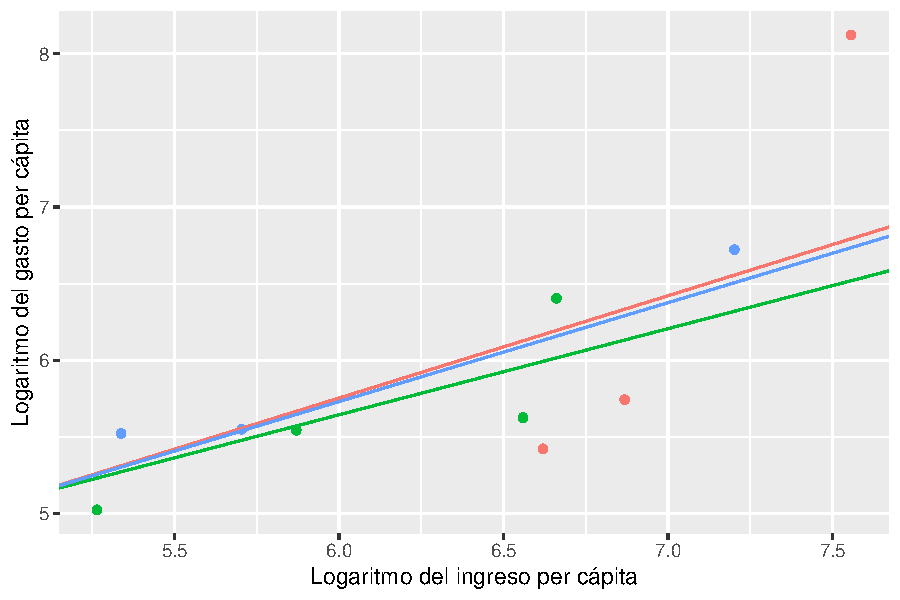
\includegraphics[width=0.7\linewidth,height=\textheight,keepaspectratio]{chapters/../figures/fig-slope-random-1.pdf}

}

\caption{\label{fig-slope-random}Rectas de regresión estimadas por
estrato: modelo con intercepto y pendiente aleatoria}

\end{figure}%

\section{Modelo logístico multinivel}\label{sec-logistica-multinivel}

En las secciones anteriores se modeló el gasto per cápita como una
variable continua. Aquí el interés pasa a un resultado binario: la
condición de pobreza del hogar. Un modelo logístico multinivel permite
relacionar la probabilidad de pobreza con características del hogar y, a
la vez, representar las diferencias entre estratos mediante efectos
aleatorios. Para estimar estos modelos se preparan primero los pesos que
se usarán en el análisis.

Para los modelos logísticos de esta sección se reconstruyen los pesos
\emph{q-weighted} utilizando el logaritmo del gasto per cápita y el
tamaño del hogar como predictores, de acuerdo con su especificación. El
siguiente código computacional realiza ese ajuste y calcula los pesos
como el cociente entre \texttt{wk} y sus valores predichos, que deben
ser finitos y positivos. También define
\texttt{reference\_household\_size} como la mediana del tamaño del
hogar, que se mantendrá fija al representar las probabilidades
predichas.

\begin{Shaded}
\begin{Highlighting}[]
\NormalTok{logistic\_weight\_model }\OtherTok{\textless{}{-}} \FunctionTok{lm}\NormalTok{(wk }\SpecialCharTok{\textasciitilde{}}\NormalTok{ log\_expenditure }\SpecialCharTok{+}\NormalTok{ household\_size, }\AttributeTok{data =}\NormalTok{ survey\_data)}
\NormalTok{logistic\_predicted\_weights }\OtherTok{\textless{}{-}} \FunctionTok{predict}\NormalTok{(logistic\_weight\_model)}
\NormalTok{survey\_data}\SpecialCharTok{$}\NormalTok{qk }\OtherTok{\textless{}{-}}\NormalTok{ survey\_data}\SpecialCharTok{$}\NormalTok{wk }\SpecialCharTok{/}\NormalTok{ logistic\_predicted\_weights}
\NormalTok{reference\_household\_size }\OtherTok{\textless{}{-}} \FunctionTok{median}\NormalTok{(survey\_data}\SpecialCharTok{$}\NormalTok{household\_size)}
\end{Highlighting}
\end{Shaded}

De acuerdo con Snijders y Bosker (\citeproc{ref-snijders2011}{2011}) y
Rabe-Hesketh y Skrondal
(\citeproc{ref-rabehesketh2012multilevel}{2012}), los modelos logísticos
multinivel constituyen una extensión de los modelos multinivel para
variables continuas al caso en que la variable respuesta es dicotómica.
En lugar de modelar directamente el valor esperado de una variable
continua, estos modelos estiman la probabilidad de ocurrencia de un
evento, incorporando simultáneamente covariables individuales y efectos
aleatorios asociados a los grupos de pertenencia. En el contexto de
encuestas de hogares, esta formulación es especialmente útil cuando se
analizan resultados binarios, como encontrarse o no en condición de
pobreza, acceder o no a un servicio, participar o no en el mercado
laboral, o presentar determinada característica sociodemográfica.

Al igual que en los modelos multinivel para variables continuas, el
punto de partida consiste en reconocer que las unidades de observación
no son independientes cuando pertenecen a un mismo grupo sustantivo.
Como se advirtió al inicio, un estrato, conglomerado o dominio del
diseño solo debe emplearse como nivel aleatorio cuando corresponda al
contexto que se desea modelar y el supuesto de efectos intercambiables
sea defendible. Sin embargo, en el caso logístico la respuesta no se
representa mediante una distribución normal con un error residual
aditivo, sino mediante una distribución Bernoulli condicional a la
probabilidad de ocurrencia del evento. Esta probabilidad se vincula con
los predictores a través de la función logit, lo que permite expresar el
modelo en una escala lineal.

\[
y_{kj} \mid \pi_{kj} \sim \text{Bernoulli}(\pi_{kj})
\]

donde \(y_{kj}\) toma el valor uno si la unidad \(k\) del estrato \(j\)
presenta el evento de interés y cero en caso contrario. La probabilidad
condicional del evento se denota por \(\pi_{kj}=Pr(y_{kj}=1)\) y se
relaciona con el predictor lineal mediante

\[
\text{logit}(\pi_{kj}) =
\log\left(\frac{\pi_{kj}}{1-\pi_{kj}}\right)
= \eta_{kj}
\]

En esta formulación, las \emph{odds} son la razón
\(\pi_{kj}/(1-\pi_{kj})\) entre la probabilidad de pobreza y la de no
pobreza. Los \emph{log-odds} son el logaritmo natural de esa razón y
coinciden con el logit, \(\eta_{kj}\). Los efectos fijos y aleatorios
actúan sobre esta escala, no directamente sobre la probabilidad. La
transformación inversa,
\(\pi_{kj}=\exp(\eta_{kj})/[1+\exp(\eta_{kj})]\), permite obtener
probabilidades. Por tanto, un cambio de una unidad en los log-odds no
equivale a un cambio de un punto porcentual en la probabilidad. La
figura~\ref{fig-logit-poverty-expenditure}, obtenida con el siguiente
código computacional, presenta la relación entre el logaritmo del gasto
per cápita y la probabilidad de pobreza, con una curva logística
ajustada.

\begin{Shaded}
\begin{Highlighting}[]
\NormalTok{pooled\_logit\_model }\OtherTok{\textless{}{-}} \FunctionTok{glm}\NormalTok{(}
\NormalTok{  poor }\SpecialCharTok{\textasciitilde{}}\NormalTok{ log\_expenditure }\SpecialCharTok{+}\NormalTok{ household\_size,}
  \AttributeTok{data =}\NormalTok{ survey\_data,}
  \AttributeTok{family =} \FunctionTok{binomial}\NormalTok{(}\AttributeTok{link =} \StringTok{"logit"}\NormalTok{)}
\NormalTok{)}
\NormalTok{pooled\_prediction\_data }\OtherTok{\textless{}{-}} \FunctionTok{tibble}\NormalTok{(}
  \AttributeTok{log\_expenditure =} \FunctionTok{seq}\NormalTok{(}
    \FunctionTok{min}\NormalTok{(survey\_data}\SpecialCharTok{$}\NormalTok{log\_expenditure),}
    \FunctionTok{max}\NormalTok{(survey\_data}\SpecialCharTok{$}\NormalTok{log\_expenditure),}
    \AttributeTok{length.out =} \DecValTok{100}
\NormalTok{  ),}
  \AttributeTok{household\_size =}\NormalTok{ reference\_household\_size}
\NormalTok{) }\SpecialCharTok{\%\textgreater{}\%}
  \FunctionTok{mutate}\NormalTok{(}
    \AttributeTok{probability =} \FunctionTok{predict}\NormalTok{(}
\NormalTok{      pooled\_logit\_model,}
      \AttributeTok{newdata =}\NormalTok{ .,}
      \AttributeTok{type =} \StringTok{"response"}
\NormalTok{    )}
\NormalTok{  )}
\FunctionTok{ggplot}\NormalTok{(pooled\_prediction\_data, }\FunctionTok{aes}\NormalTok{(log\_expenditure, probability)) }\SpecialCharTok{+}
  \FunctionTok{geom\_line}\NormalTok{() }\SpecialCharTok{+}
  \FunctionTok{labs}\NormalTok{(}\AttributeTok{y =} \StringTok{"Probabilidad de pobreza"}\NormalTok{, }\AttributeTok{x =} \StringTok{"Logaritmo del gasto per cápita"}\NormalTok{)}
\end{Highlighting}
\end{Shaded}

\begin{figure}[H]

\centering{

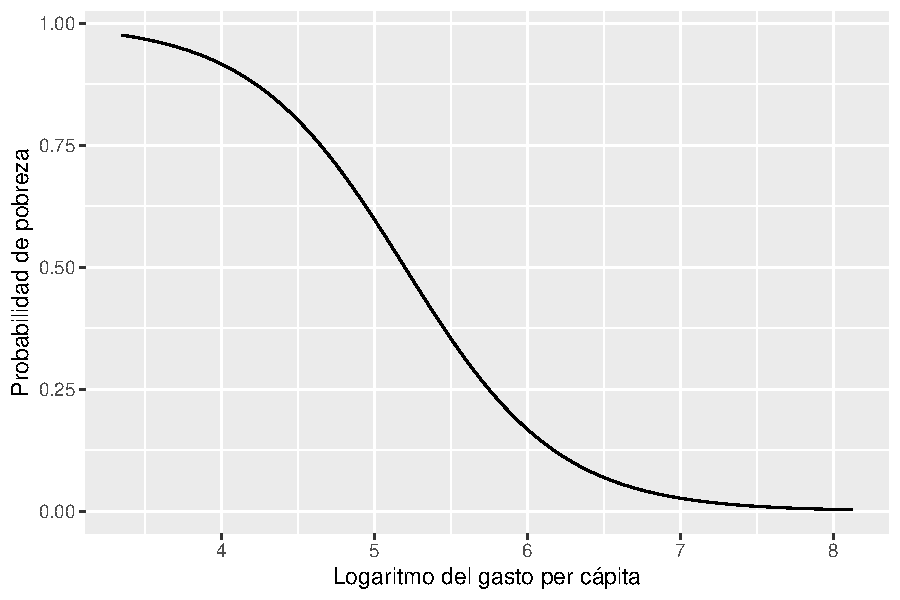
\includegraphics[width=0.7\linewidth,height=\textheight,keepaspectratio]{chapters/../figures/fig-logit-poverty-expenditure-1.pdf}

}

\caption{\label{fig-logit-poverty-expenditure}Probabilidad de pobreza
según el logaritmo del gasto, controlando por el tamaño del hogar}

\end{figure}%

La curva ajustada corresponde a un modelo logístico sin efectos
aleatorios ni ponderación, utilizado como referencia inicial.
Manteniendo el tamaño del hogar en 4 integrantes, la probabilidad
estimada de pobreza disminuye al aumentar el gasto per cápita. La
inclusión del tamaño del hogar permite describir esta asociación
comparando hogares con igual número de integrantes. Los modelos
siguientes incorporan los estratos y los pesos ilustrativos
\emph{q-weighted}.

\subsection{Modelo nulo logístico}\label{modelo-nulo-logistico}

Según Snijders y Bosker (\citeproc{ref-snijders2011}{2011}), como en el
caso de variables continuas, el modelo nulo logístico constituye el
punto de partida para estudiar la estructura jerárquica de la variable
respuesta. Este modelo no incorpora covariables y permite evaluar si la
probabilidad promedio del evento varía entre estratos. En el ejemplo
considerado, el evento de interés corresponde a la condición de pobreza,
de modo que el modelo permite separar la heterogeneidad atribuible a
diferencias entre estratos de la variación individual propia de una
respuesta binaria.

En el modelo nulo, la variable de interés sigue la siguiente
distribución Bernoulli:

\[
y_{kj} \mid \pi_{kj} \sim \text{Bernoulli}(\pi_{kj})
\]

En donde la probabilidad de éxito para la unidad \(k\) perteneciente al
grupo \(j\) se modela mediante

\begin{equation}\protect\phantomsection\label{eq-modelo-logistico-multinivel}{
\text{logit}(\pi_{kj}) = \beta_{0j},
}\end{equation}

donde \(\beta_{0j}\) representa el intercepto específico del estrato
\(j\) en escala logit. A su vez, dicho intercepto se descompone como

\[
\beta_{0j} = \gamma_{00} + \tau_{0j}
\]

siendo \(\gamma_{00}\) el intercepto promedio global de la población y
\(\tau_{0j}\) el efecto aleatorio asociado al estrato \(j\), el cual
captura las desviaciones de cada grupo respecto al promedio general. Al
igual que en el modelo nulo para variables continuas, este efecto
aleatorio permite modelar explícitamente la heterogeneidad entre grupos:

\[
\tau_{0j} \sim N(0,\sigma_{\tau}^{2})
\]

De acuerdo con Merlo et~al. (\citeproc{ref-merlo2006brief}{2006}), a
diferencia del modelo lineal multinivel, aquí no se incorpora un término
residual aditivo \(\epsilon_{kj}\) en la ecuación del nivel individual.
La variabilidad interna en el grupo está determinada por la distribución
Bernoulli de la respuesta. Para cuantificar la dependencia entre
unidades pertenecientes al mismo estrato, puede utilizarse el enfoque de
variable latente, bajo el cual esta varianza residual se aproxima por la
varianza de la distribución logística estándar, es decir, \(\pi^2/3\).
Así, la correlación intraclase del modelo logístico se expresa como

\begin{equation}\protect\phantomsection\label{eq-cci-logistico}{
\rho =
\frac{\sigma_\tau^2}
{\sigma_\tau^2 + \frac{\pi^2}{3}}
}\end{equation}

Un valor elevado de ICC indica que la probabilidad del evento presenta
una estructura de agrupamiento importante, es decir, que dos unidades
pertenecientes al mismo estrato tienden a parecerse más entre sí que dos
unidades tomadas de estratos distintos. En contraste, un valor bajo
sugiere que la mayor parte de la variación se concentra a nivel
individual. Este ICC es una medida en escala latente y no equivale
directamente a una correlación de respuestas binarias observadas. El
ajuste en \texttt{R}, mediante \texttt{glmer()}, se realiza de la
siguiente manera:

\begin{Shaded}
\begin{Highlighting}[]
\NormalTok{logistic\_null\_model }\OtherTok{\textless{}{-}} \FunctionTok{glmer}\NormalTok{(}
\NormalTok{  poor }\SpecialCharTok{\textasciitilde{}}\NormalTok{ (}\DecValTok{1} \SpecialCharTok{|}\NormalTok{ Stratum),}
  \AttributeTok{data =}\NormalTok{ survey\_data,}
  \AttributeTok{weights =}\NormalTok{ qk,}
  \AttributeTok{family =} \FunctionTok{binomial}\NormalTok{(}\AttributeTok{link =} \StringTok{"logit"}\NormalTok{)}
\NormalTok{)}

\NormalTok{logistic\_null\_model\_icc }\OtherTok{\textless{}{-}}\NormalTok{ performance}\SpecialCharTok{::}\FunctionTok{icc}\NormalTok{(logistic\_null\_model)}
\NormalTok{logistic\_null\_model\_icc}
\end{Highlighting}
\end{Shaded}

La correlación intraclase del modelo nulo logístico es de 0,056. Este
valor resume la variación entre estratos en la escala latente del
modelo; no representa una proporción de la varianza observada de las
respuestas binarias. El siguiente código computacional extrae y organiza
los interceptos por estrato del modelo logístico nulo.

\begin{Shaded}
\begin{Highlighting}[]
\NormalTok{null\_logistic\_intercepts\_table }\OtherTok{\textless{}{-}} \FunctionTok{coef}\NormalTok{(logistic\_null\_model)}\SpecialCharTok{$}\NormalTok{Stratum }\SpecialCharTok{\%\textgreater{}\%}
\NormalTok{  tibble}\SpecialCharTok{::}\FunctionTok{rownames\_to\_column}\NormalTok{(}\StringTok{"stratum"}\NormalTok{) }\SpecialCharTok{\%\textgreater{}\%}
  \FunctionTok{slice}\NormalTok{(}\DecValTok{1}\SpecialCharTok{:}\DecValTok{5}\NormalTok{L) }\SpecialCharTok{\%\textgreater{}\%}
  \FunctionTok{transmute}\NormalTok{(stratum, }\AttributeTok{intercept =}\NormalTok{ .data[[}\StringTok{"(Intercept)"}\NormalTok{]])}

\NormalTok{null\_logistic\_intercepts\_table}
\end{Highlighting}
\end{Shaded}

{

\begin{longtable}[]{@{}lr@{}}

\caption{\label{tbl-coef-logit-nulo}Interceptos estimados por estrato en
el modelo logístico nulo (primeros 5 estratos)}

\tabularnewline

\toprule\noalign{}
Estrato & Intercepto (beta) \\
\midrule\noalign{}
\endhead
\bottomrule\noalign{}
\endlastfoot
idStrt001 & -0.724 \\
idStrt002 & -0.504 \\
idStrt003 & -0.913 \\
idStrt004 & -1.002 \\
idStrt005 & -0.851 \\

\end{longtable}

}

Los coeficientes del modelo nulo logístico por estrato se presentan en
la tabla~\ref{tbl-coef-logit-nulo}. Los interceptos de los primeros 5
estratos son negativos. Entre ellos, idStrt004 presenta el menor
intercepto (aproximadamente -1,002), equivalente a una probabilidad de
pobreza de 0,269; idStrt002 presenta el mayor (aproximadamente -0,504),
equivalente a una probabilidad de 0,377. Estas probabilidades se
obtienen aplicando la función logística a los interceptos.

\subsection{Modelo logístico con intercepto
aleatorio}\label{modelo-logistico-con-intercepto-aleatorio}

De acuerdo con Snijders y Bosker (\citeproc{ref-snijders2011}{2011}) y
Rabe-Hesketh y Skrondal
(\citeproc{ref-rabehesketh2012multilevel}{2012}), el modelo logístico
con intercepto aleatorio incorpora covariables individuales o del hogar,
permitiendo que el nivel base del evento varíe entre estratos. Su lógica
es paralela a la del modelo con intercepto aleatorio para variables
continuas: los efectos de las covariables se consideran comunes a todos
los grupos, mientras que cada estrato puede tener su propio intercepto.
En este caso, las diferencias entre interceptos se interpretan como
diferencias en los \emph{log-odds} base del evento.

El modelo se expresa como
\(y_{kj} \mid \pi_{kj} \sim \text{Bernoulli}(\pi_{kj})\). En donde
\(\text{logit}(\pi_{kj}) = \beta_{0j} + \mathbf{x}_{kj}\boldsymbol{\beta}\)
y \(\beta_{0j} = \gamma_{00} + \tau_{0j}\). En este caso,
\(\mathbf{x}_{kj}\) representa el vector de covariables de la unidad
\(k\) en el estrato \(j\), \(\boldsymbol{\beta}\) es el vector de
efectos fijos comunes a todos los estratos y \(\tau_{0j}\) captura la
desviación específica del estrato respecto al intercepto promedio
global. Como antes, se asume que
\(\tau_{0j} \sim N(0,\sigma_{\tau}^{2})\).

Bajo esta especificación, dos estratos con los mismos valores de las
covariables pueden presentar probabilidades base distintas del evento
debido a sus interceptos aleatorios. Sin embargo, el efecto de cada
covariable sobre la escala logit se mantiene constante entre estratos.
En el ejemplo, esto equivale a permitir que la probabilidad base de
pobreza cambie entre estratos, mientras que la asociación entre el
logaritmo del gasto per cápita y la pobreza se estima controlando por el
tamaño del hogar. Ambas pendientes son comunes a todos los estratos. El
siguiente código computacional ajusta el modelo logístico con intercepto
aleatorio y calcula su correlación intraclase.

\begin{Shaded}
\begin{Highlighting}[]
\NormalTok{random\_intercept\_logit\_model }\OtherTok{\textless{}{-}} \FunctionTok{glmer}\NormalTok{(}
\NormalTok{  poor }\SpecialCharTok{\textasciitilde{}}\NormalTok{ log\_expenditure }\SpecialCharTok{+}\NormalTok{ household\_size }\SpecialCharTok{+}\NormalTok{ (}\DecValTok{1} \SpecialCharTok{|}\NormalTok{ Stratum),}
  \AttributeTok{data =}\NormalTok{ survey\_data,}
  \AttributeTok{family =} \FunctionTok{binomial}\NormalTok{(}\AttributeTok{link =} \StringTok{"logit"}\NormalTok{),}
  \AttributeTok{weights =}\NormalTok{ qk}
\NormalTok{)}

\NormalTok{random\_intercept\_logit\_model\_icc }\OtherTok{\textless{}{-}}\NormalTok{ performance}\SpecialCharTok{::}\FunctionTok{icc}\NormalTok{(random\_intercept\_logit\_model)}
\NormalTok{random\_intercept\_logit\_model\_icc}
\end{Highlighting}
\end{Shaded}

Después de incorporar el logaritmo del gasto per cápita y el tamaño del
hogar, la correlación intraclase ajustada es de 0,058. Este indicador
resume el agrupamiento residual en la escala latente; su comparación con
el modelo nulo no debe interpretarse como una proporción de variabilidad
explicada por las covariables.

La tabla~\ref{tbl-coef-logit-int-aleatorio} presenta en columnas
separadas los coeficientes comunes y los interceptos específicos de los
primeros cinco estratos. Para iguales valores de gasto y tamaño del
hogar, un intercepto mayor corresponde a una probabilidad más alta. El
intercepto se refiere a un gasto de una unidad monetaria y un hogar de
cero integrantes, valores ajenos a los perfiles observados; por ello, no
representa una probabilidad habitual de pobreza. La columna OR
condicional presenta la exponencial de cada pendiente. Se denomina
condicional porque compara las odds de pobreza de dos hogares dentro del
mismo estrato, manteniendo fijos los efectos aleatorios del estrato y
las demás covariables. Por tanto, describe una asociación dentro del
estrato y no un OR marginal obtenido al promediar las probabilidades
sobre toda la población. Un OR menor que uno indica menores odds y uno
mayor que uno indica mayores odds; no es una razón de probabilidades ni
una diferencia en puntos porcentuales.

El coeficiente de \texttt{log\_expenditure} representa la elasticidad de
las odds de pobreza respecto al gasto, manteniendo constantes el tamaño
del hogar y el efecto del estrato. Su estimación es -2,252. Manteniendo
constantes el tamaño del hogar y el efecto del estrato, un aumento del
10 \% en el gasto per cápita multiplica las odds de pobreza por
\(1.1^{\hat{\beta}}\), donde \(\hat{\beta}\) es el coeficiente estimado
de \texttt{log\_expenditure}. En este modelo, el factor es 0,807. Es
decir, las odds quedan en 80,7 \% de su valor inicial. La reducción
porcentual se calcula como \(100[1-1.1^{\hat{\beta}}]\) y es
aproximadamente 19,3 \%.

El coeficiente del tamaño del hogar es 0,631. Para un mismo gasto per
cápita y estrato, cada integrante adicional multiplica las odds por
1,879. Estas asociaciones no establecen causalidad y los cambios en las
odds no equivalen a cambios porcentuales de igual magnitud en la
probabilidad.

Para \texttt{household\_size}, el OR corresponde a un integrante
adicional, manteniendo constante el gasto per cápita. Para
\texttt{log\_expenditure}, corresponde a una unidad adicional del
logaritmo natural, es decir, a multiplicar el gasto por \(e\),
manteniendo fijo el tamaño del hogar. Si se desea interpretar un aumento
del 10 \% en el gasto, el OR correspondiente es
\(\exp[\beta\log(1.1)]=1.1^\beta\), como en el cálculo anterior. En este
modelo, las pendientes son comunes a todos los estratos y, por ello,
también lo son sus OR, aunque las probabilidades de partida difieran.
Los interceptos llevan un guion en esta columna: su exponencial expresa
odds de referencia y no un odds ratio. El siguiente código computacional
dispone en columnas los coeficientes y sus OR condicionales para cada
uno de los primeros cinco estratos.

\begin{Shaded}
\begin{Highlighting}[]
\NormalTok{random\_logistic\_intercept\_coefficients\_table }\OtherTok{\textless{}{-}} \FunctionTok{coef}\NormalTok{(random\_intercept\_logit\_model)}\SpecialCharTok{$}\NormalTok{Stratum }\SpecialCharTok{\%\textgreater{}\%}
\NormalTok{  tibble}\SpecialCharTok{::}\FunctionTok{rownames\_to\_column}\NormalTok{(}\StringTok{"stratum"}\NormalTok{) }\SpecialCharTok{\%\textgreater{}\%}
  \FunctionTok{slice}\NormalTok{(}\DecValTok{1}\SpecialCharTok{:}\DecValTok{5}\NormalTok{L) }\SpecialCharTok{\%\textgreater{}\%}
  \FunctionTok{transmute}\NormalTok{(}
\NormalTok{    stratum,}
    \AttributeTok{intercept =}\NormalTok{ .data[[}\StringTok{"(Intercept)"}\NormalTok{]],}
    \AttributeTok{expenditure\_coefficient =}\NormalTok{ log\_expenditure,}
    \AttributeTok{household\_size\_coefficient =}\NormalTok{ household\_size,}
    \AttributeTok{expenditure\_or =} \FunctionTok{exp}\NormalTok{(log\_expenditure),}
    \AttributeTok{household\_size\_or =} \FunctionTok{exp}\NormalTok{(household\_size)}
\NormalTok{  )}

\NormalTok{random\_logistic\_intercept\_coefficients\_table}
\end{Highlighting}
\end{Shaded}

{

\begin{longtable}[]{@{}
  >{\raggedright\arraybackslash}p{(\linewidth - 10\tabcolsep) * \real{0.1064}}
  >{\raggedleft\arraybackslash}p{(\linewidth - 10\tabcolsep) * \real{0.1915}}
  >{\raggedleft\arraybackslash}p{(\linewidth - 10\tabcolsep) * \real{0.1809}}
  >{\raggedleft\arraybackslash}p{(\linewidth - 10\tabcolsep) * \real{0.2128}}
  >{\raggedright\arraybackslash}p{(\linewidth - 10\tabcolsep) * \real{0.1383}}
  >{\raggedright\arraybackslash}p{(\linewidth - 10\tabcolsep) * \real{0.1702}}@{}}

\caption{\label{tbl-coef-logit-int-aleatorio}Coeficientes y OR
condicionales del modelo logístico con intercepto aleatorio (5
estratos)}

\tabularnewline

\toprule\noalign{}
\begin{minipage}[b]{\linewidth}\raggedright
Estrato
\end{minipage} & \begin{minipage}[b]{\linewidth}\raggedleft
Intercepto (beta)
\end{minipage} & \begin{minipage}[b]{\linewidth}\raggedleft
Log gasto (beta)
\end{minipage} & \begin{minipage}[b]{\linewidth}\raggedleft
Tamaño hogar (beta)
\end{minipage} & \begin{minipage}[b]{\linewidth}\raggedright
OR log gasto
\end{minipage} & \begin{minipage}[b]{\linewidth}\raggedright
OR tamaño hogar
\end{minipage} \\
\midrule\noalign{}
\endhead
\bottomrule\noalign{}
\endlastfoot
idStrt001 & 9.24 & -2.25 & 0.631 & 0.105 & 1.879 \\
idStrt002 & 9.46 & -2.25 & 0.631 & 0.105 & 1.879 \\
idStrt003 & 9.12 & -2.25 & 0.631 & 0.105 & 1.879 \\
idStrt004 & 9.24 & -2.25 & 0.631 & 0.105 & 1.879 \\
idStrt005 & 9.23 & -2.25 & 0.631 & 0.105 & 1.879 \\

\end{longtable}

}

El siguiente código computacional obtiene probabilidades predichas para
los tres estratos seleccionados. \texttt{group\_by(Stratum)} y
\texttt{reframe()} generan, para cada estrato, una secuencia de 100
valores de \texttt{log\_expenditure} entre su mínimo y su máximo
observado, fijando \texttt{household\_size} en
\texttt{reference\_household\_size}. La función \texttt{predict()}
utiliza esos valores y el efecto aleatorio del estrato para calcular las
predicciones; con \texttt{type\ =\ "response"}, el resultado se expresa
como probabilidad de pobreza.

\begin{Shaded}
\begin{Highlighting}[]
\NormalTok{prediction\_data }\OtherTok{\textless{}{-}}\NormalTok{ plot\_data }\SpecialCharTok{\%\textgreater{}\%}
  \FunctionTok{group\_by}\NormalTok{(Stratum) }\SpecialCharTok{\%\textgreater{}\%}
  \FunctionTok{reframe}\NormalTok{(}
    \AttributeTok{log\_expenditure =} \FunctionTok{seq}\NormalTok{(}
      \FunctionTok{min}\NormalTok{(log\_expenditure),}
      \FunctionTok{max}\NormalTok{(log\_expenditure),}
      \AttributeTok{length.out =} \DecValTok{100}
\NormalTok{    ),}
    \AttributeTok{household\_size =}\NormalTok{ reference\_household\_size}
\NormalTok{  ) }\SpecialCharTok{\%\textgreater{}\%}
  \FunctionTok{mutate}\NormalTok{(}
    \AttributeTok{probability =} \FunctionTok{predict}\NormalTok{(}
\NormalTok{      random\_intercept\_logit\_model,}
      \AttributeTok{newdata =}\NormalTok{ .,}
      \AttributeTok{type =} \StringTok{"response"}
\NormalTok{    )}
\NormalTok{  )}
\end{Highlighting}
\end{Shaded}

La figura~\ref{fig-logit-interaction-random}, obtenida con el siguiente
código computacional, muestra las probabilidades predichas según el
logaritmo del gasto para hogares de 4 integrantes en los tres estratos
seleccionados. Las curvas son decrecientes y comparten una pendiente en
la escala logit; sus diferencias reflejan los interceptos específicos de
cada estrato.

\begin{Shaded}
\begin{Highlighting}[]
\FunctionTok{ggplot}\NormalTok{(}
  \AttributeTok{data =}\NormalTok{ prediction\_data,}
  \FunctionTok{aes}\NormalTok{(}
    \AttributeTok{y =}\NormalTok{ probability,}
    \AttributeTok{x =}\NormalTok{ log\_expenditure,}
    \AttributeTok{colour =}\NormalTok{ Stratum}
\NormalTok{  )}
\NormalTok{) }\SpecialCharTok{+}
  \FunctionTok{geom\_line}\NormalTok{() }\SpecialCharTok{+}
  \FunctionTok{labs}\NormalTok{(}\AttributeTok{y =} \StringTok{"Probabilidad de pobreza"}\NormalTok{, }\AttributeTok{x =} \StringTok{"Logaritmo del gasto per cápita"}\NormalTok{) }\SpecialCharTok{+}
  \FunctionTok{theme}\NormalTok{(}\AttributeTok{legend.position =} \StringTok{"none"}\NormalTok{)}
\end{Highlighting}
\end{Shaded}

\begin{figure}[H]

\centering{

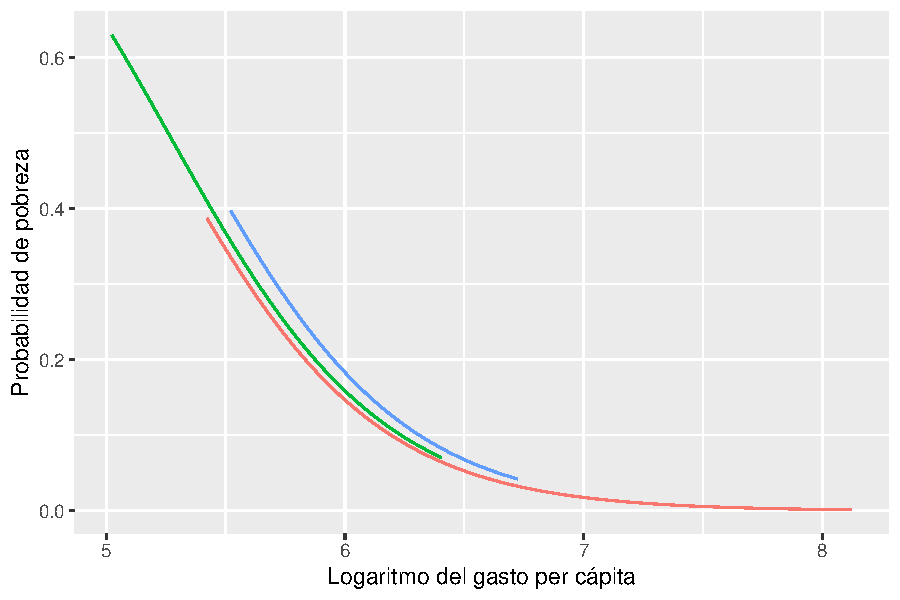
\includegraphics[width=0.7\linewidth,height=\textheight,keepaspectratio]{chapters/../figures/fig-logit-interaction-random-1.pdf}

}

\caption{\label{fig-logit-interaction-random}Curvas de probabilidad
predichas por estrato: modelo logístico con intercepto aleatorio}

\end{figure}%

\subsection{Modelo logístico con intercepto y pendiente
aleatoria}\label{modelo-logistico-con-intercepto-y-pendiente-aleatoria}

El modelo logístico con intercepto y pendiente aleatoria extiende la
especificación anterior permitiendo que no sólo varíe el nivel base del
evento entre estratos, sino también el efecto de una covariable
específica. Esta formulación es análoga al modelo de intercepto y
pendiente aleatorios para variables continuas, con la salvedad de que
las diferencias entre estratos se expresan en la escala logit y se
traducen en curvas de probabilidad no lineales.

Sea \(x_{kj}\) la covariable cuyo efecto se permite variar entre
estratos, y sea \(\mathbf{z}_{kj}\) el conjunto de covariables con
efectos fijos comunes. En este modelo, la probabilidad de éxito se asume
de tal forma que
\(\text{logit}(\pi_{kj}) = \beta_{0j} + x_{kj}\beta_{1j} + \mathbf{z}_{kj}\boldsymbol{\beta}\).
En donde, \(\beta_{0j}\) es el intercepto específico del estrato \(j\) y
\(\beta_{1j}\) es la pendiente específica asociada a la covariable
\(x_{kj}\).

Ambos parámetros se descomponen en una parte promedio poblacional y una
desviación específica del estrato, de tal manera que
\(\beta_{0j} = \gamma_{00} + \tau_{0j}\) y
\(\beta_{1j} = \gamma_{10} + \tau_{1j}\). En donde los términos
\(\gamma_{00}\) y \(\gamma_{10}\) representan, respectivamente, el
intercepto promedio global y la pendiente promedio global en escala
logit. Por su parte, \(\tau_{0j}\) y \(\tau_{1j}\) capturan cuánto se
aparta el estrato \(j\) de esos promedios. En este ejemplo, \(x_{kj}\)
es el logaritmo del gasto per cápita, cuya pendiente varía entre
estratos, y el tamaño del hogar se incorpora como covariable con efecto
fijo común. El siguiente código computacional ajusta el modelo y calcula
sus diagnósticos:

\begin{Shaded}
\begin{Highlighting}[]
\NormalTok{random\_slope\_logit\_model }\OtherTok{\textless{}{-}} \FunctionTok{glmer}\NormalTok{(}
\NormalTok{  poor }\SpecialCharTok{\textasciitilde{}}\NormalTok{ log\_expenditure }\SpecialCharTok{+}\NormalTok{ household\_size }\SpecialCharTok{+}\NormalTok{ (}\DecValTok{1} \SpecialCharTok{+}\NormalTok{ log\_expenditure }\SpecialCharTok{|}\NormalTok{ Stratum),}
  \AttributeTok{data =}\NormalTok{ survey\_data,}
  \AttributeTok{weights =}\NormalTok{ qk,}
  \AttributeTok{family =} \FunctionTok{binomial}\NormalTok{(}\AttributeTok{link =} \StringTok{"logit"}\NormalTok{)}
\NormalTok{)}

\NormalTok{random\_slope\_logit\_model}
\end{Highlighting}
\end{Shaded}

La tabla~\ref{tbl-coef-logit-pendiente} presenta los coeficientes y OR
condicionales de los primeros cinco estratos en columnas separadas. Para
el logaritmo del gasto, la pendiente del estrato \(j\) es
\(\beta_{1j}=\gamma_{10}+\tau_{1j}\), de modo que su OR es
\(\exp(\gamma_{10}+\tau_{1j})\). Se exponencia la pendiente completa que
devuelve \texttt{coef()}, que combina el efecto fijo y la desviación
aleatoria del estrato. Este OR compara hogares del mismo tamaño dentro
de ese estrato y corresponde a multiplicar el gasto por \(e\); para un
aumento del 10 \%, se utiliza \(1.1^{\beta_{1j}}\). El OR del tamaño del
hogar se mantiene común porque su pendiente es fija. Las diferencias
entre los OR del gasto son estimaciones condicionales del modelo y deben
interpretarse con cautela. El siguiente código computacional presenta en
columnas separadas los coeficientes de cada estrato y los OR
condicionales correspondientes.

\begin{Shaded}
\begin{Highlighting}[]
\NormalTok{random\_logistic\_slope\_coefficients\_table }\OtherTok{\textless{}{-}} \FunctionTok{coef}\NormalTok{(random\_slope\_logit\_model)}\SpecialCharTok{$}\NormalTok{Stratum }\SpecialCharTok{\%\textgreater{}\%}
\NormalTok{  tibble}\SpecialCharTok{::}\FunctionTok{rownames\_to\_column}\NormalTok{(}\StringTok{"stratum"}\NormalTok{) }\SpecialCharTok{\%\textgreater{}\%}
  \FunctionTok{slice}\NormalTok{(}\DecValTok{1}\SpecialCharTok{:}\DecValTok{5}\NormalTok{L) }\SpecialCharTok{\%\textgreater{}\%}
  \FunctionTok{transmute}\NormalTok{(}
\NormalTok{    stratum,}
    \AttributeTok{intercept =}\NormalTok{ .data[[}\StringTok{"(Intercept)"}\NormalTok{]],}
    \AttributeTok{expenditure\_coefficient =}\NormalTok{ log\_expenditure,}
    \AttributeTok{household\_size\_coefficient =}\NormalTok{ household\_size,}
    \AttributeTok{expenditure\_or =} \FunctionTok{exp}\NormalTok{(log\_expenditure),}
    \AttributeTok{household\_size\_or =} \FunctionTok{exp}\NormalTok{(household\_size)}
\NormalTok{  )}

\NormalTok{random\_logistic\_slope\_coefficients\_table}
\end{Highlighting}
\end{Shaded}

{

\begin{longtable}[]{@{}
  >{\raggedright\arraybackslash}p{(\linewidth - 10\tabcolsep) * \real{0.1064}}
  >{\raggedleft\arraybackslash}p{(\linewidth - 10\tabcolsep) * \real{0.1915}}
  >{\raggedleft\arraybackslash}p{(\linewidth - 10\tabcolsep) * \real{0.1809}}
  >{\raggedleft\arraybackslash}p{(\linewidth - 10\tabcolsep) * \real{0.2128}}
  >{\raggedright\arraybackslash}p{(\linewidth - 10\tabcolsep) * \real{0.1383}}
  >{\raggedright\arraybackslash}p{(\linewidth - 10\tabcolsep) * \real{0.1702}}@{}}

\caption{\label{tbl-coef-logit-pendiente}Coeficientes y OR condicionales
del modelo logístico con pendiente aleatoria (5 estratos)}

\tabularnewline

\toprule\noalign{}
\begin{minipage}[b]{\linewidth}\raggedright
Estrato
\end{minipage} & \begin{minipage}[b]{\linewidth}\raggedleft
Intercepto (beta)
\end{minipage} & \begin{minipage}[b]{\linewidth}\raggedleft
Log gasto (beta)
\end{minipage} & \begin{minipage}[b]{\linewidth}\raggedleft
Tamaño hogar (beta)
\end{minipage} & \begin{minipage}[b]{\linewidth}\raggedright
OR log gasto
\end{minipage} & \begin{minipage}[b]{\linewidth}\raggedright
OR tamaño hogar
\end{minipage} \\
\midrule\noalign{}
\endhead
\bottomrule\noalign{}
\endlastfoot
idStrt001 & 9.17 & -2.22 & 0.633 & 0.109 & 1.883 \\
idStrt002 & 10.37 & -2.40 & 0.633 & 0.090 & 1.883 \\
idStrt003 & 7.94 & -2.03 & 0.633 & 0.131 & 1.883 \\
idStrt004 & 8.94 & -2.19 & 0.633 & 0.112 & 1.883 \\
idStrt005 & 9.19 & -2.22 & 0.633 & 0.108 & 1.883 \\

\end{longtable}

}

El componente fijo de la elasticidad de las odds de pobreza respecto al
gasto es -2,243. Las pendientes condicionales por estrato van de -2,803
a -1,824: todas son negativas en este ajuste. El coeficiente común del
tamaño del hogar es 0,633. Cada pendiente específica representa la
variación porcentual aproximada de las odds ante un aumento del 1 \% en
el gasto dentro del estrato, manteniendo fijo el tamaño del hogar. No
representa una elasticidad constante de la probabilidad de pobreza.

El siguiente código computacional calcula las probabilidades para
distintos valores del logaritmo del gasto dentro de cada estrato,
manteniendo el tamaño del hogar en la misma mediana utilizada en el
gráfico anterior.

\begin{Shaded}
\begin{Highlighting}[]
\NormalTok{prediction\_data }\OtherTok{\textless{}{-}}\NormalTok{ plot\_data }\SpecialCharTok{\%\textgreater{}\%}
  \FunctionTok{group\_by}\NormalTok{(Stratum) }\SpecialCharTok{\%\textgreater{}\%}
  \FunctionTok{reframe}\NormalTok{(}
    \AttributeTok{log\_expenditure =} \FunctionTok{seq}\NormalTok{(}
      \FunctionTok{min}\NormalTok{(log\_expenditure),}
      \FunctionTok{max}\NormalTok{(log\_expenditure),}
      \AttributeTok{length.out =} \DecValTok{100}
\NormalTok{    ),}
    \AttributeTok{household\_size =}\NormalTok{ reference\_household\_size}
\NormalTok{  ) }\SpecialCharTok{\%\textgreater{}\%}
  \FunctionTok{mutate}\NormalTok{(}
    \AttributeTok{probability =} \FunctionTok{predict}\NormalTok{(}
\NormalTok{      random\_slope\_logit\_model,}
      \AttributeTok{newdata =}\NormalTok{ .,}
      \AttributeTok{type =} \StringTok{"response"}
\NormalTok{    )}
\NormalTok{  )}
\end{Highlighting}
\end{Shaded}

La figura~\ref{fig-logit-slope-random}, obtenida con el siguiente código
computacional, muestra las curvas predichas para hogares de 4
integrantes. Las curvas descendentes reflejan la asociación negativa
entre gasto per cápita y pobreza, controlando por tamaño del hogar.

\begin{Shaded}
\begin{Highlighting}[]
\FunctionTok{ggplot}\NormalTok{(}
  \AttributeTok{data =}\NormalTok{ prediction\_data,}
  \FunctionTok{aes}\NormalTok{(}
    \AttributeTok{y =}\NormalTok{ probability,}
    \AttributeTok{x =}\NormalTok{ log\_expenditure,}
    \AttributeTok{colour =}\NormalTok{ Stratum}
\NormalTok{  )}
\NormalTok{) }\SpecialCharTok{+}
  \FunctionTok{geom\_line}\NormalTok{() }\SpecialCharTok{+}
  \FunctionTok{labs}\NormalTok{(}
    \AttributeTok{y =} \StringTok{"Probabilidad de pobreza"}\NormalTok{,}
    \AttributeTok{x =} \StringTok{"Logaritmo del gasto per cápita"}
\NormalTok{  ) }\SpecialCharTok{+}
  \FunctionTok{theme}\NormalTok{(}\AttributeTok{legend.position =} \StringTok{"none"}\NormalTok{)}
\end{Highlighting}
\end{Shaded}

\begin{figure}[H]

\centering{

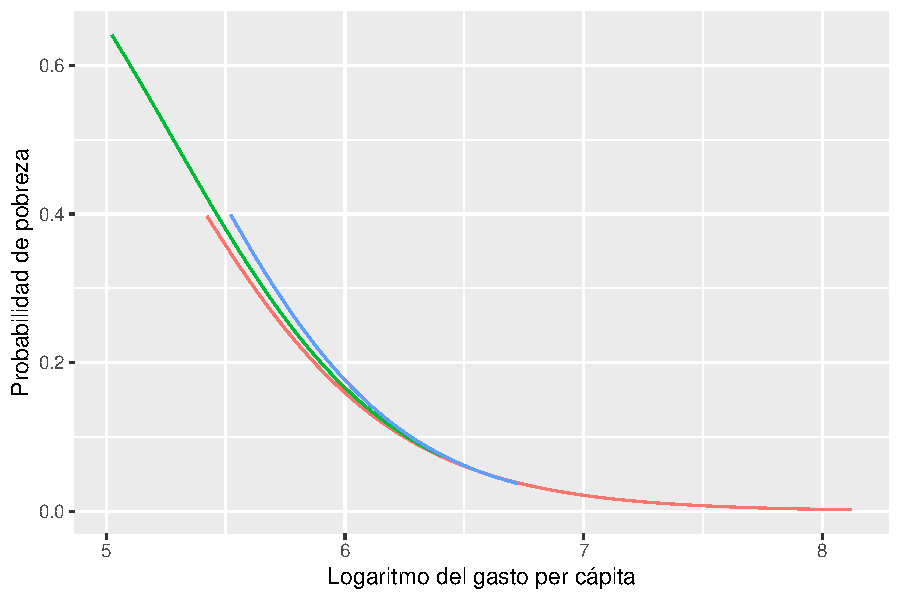
\includegraphics[width=0.7\linewidth,height=\textheight,keepaspectratio]{chapters/../figures/fig-logit-slope-random-1.pdf}

}

\caption{\label{fig-logit-slope-random}Curvas de probabilidad predichas
por estrato: modelo logístico con intercepto y pendiente aleatoria}

\end{figure}%

\part{Anexos}

\chapter{\texorpdfstring{Manejo de bases de datos con
\texttt{R}}{Manejo de bases de datos con R}}\label{ap1}

\texttt{R} es un software estadístico ampliamente utilizado para el
análisis de datos y la generación de gráficos y permite un ambiente
integrado para el análisis estadístico, en particular de bases de datos
(\citeproc{ref-RCoreTeam2026}{R Core Team 2026a}). Esto significa que
permite realizar procesos de análisis, programación, visualización y
manejo de datos dentro de un mismo entorno. En este anexo se utiliza el
enfoque del \texttt{tidyverse}, cuya organización de datos se relaciona
con los principios expuestos por Wickham
(\citeproc{ref-Wickham2014}{2014}), y en particular la librería
\texttt{dplyr}, para organizar una secuencia lógica de trabajo con bases
de datos: cargar la información, inspeccionarla, seleccionar variables,
filtrar registros, ordenar filas, crear variables y producir resúmenes.

\section{Preparación del entorno de
trabajo}\label{preparacion-del-entorno-de-trabajo}

Dado que \texttt{R} es un lenguaje de programación de carácter
colaborativo, permite que su comunidad de usuarios y desarrolladores
contribuya continuamente mediante la creación de funciones, paquetes y
librerías especializadas. Gracias a este ecosistema abierto, es posible
ampliar sus capacidades para distintos tipos de análisis estadístico y
procesamiento de datos. Entre las librerías más utilizadas para el
análisis de bases de datos se encuentran las siguientes:

\begin{itemize}
\item
  la librería \texttt{tidyverse} corresponde a un conjunto de paquetes
  de \texttt{R} diseñados para apoyar distintas etapas del trabajo con
  datos, desde su importación y transformación hasta su exploración,
  análisis y visualización (\citeproc{ref-tidyverse2026}{Wickham,
  Averick, et~al. 2026}). Su uso se ha extendido ampliamente en ciencia
  de datos porque ofrece una forma de trabajo consistente y ordenada.
\item
  la librería \texttt{dplyr} ofrece herramientas para organizar y
  transformar bases de datos rectangulares. Su utilidad radica en que
  reúne, en una sintaxis simple y consistente, las operaciones más
  frecuentes del trabajo analítico con datos: seleccionar variables,
  filtrar registros, crear nuevas columnas, ordenar observaciones y
  resumir información (\citeproc{ref-dplyr2026}{Wickham, François,
  et~al. 2026}).
\end{itemize}

Antes de poder utilizar las diferentes funciones que cada librería
tiene, es necesario descargarlas de antemano de la web. El comando
\texttt{install.packages} permite realizar esta tarea. Note que algunas
librerías pueden depender de otras, así que para poder utilizarlas es
necesario instalar también las dependencias adicionales.

El siguiente código reúne los paquetes utilizados en los capítulos y
apéndices del libro, incluidos los llamados mediante
\texttt{paquete::función()}. La instalación se realiza una vez por
equipo o biblioteca de \texttt{R}; \texttt{install.packages()} instala
también las dependencias necesarias. El paquete \texttt{stats} forma
parte de la instalación estándar de \texttt{R}, por lo que no se incluye
en esta descarga.

\begin{Shaded}
\begin{Highlighting}[]
\FunctionTok{install.packages}\NormalTok{(}\FunctionTok{c}\NormalTok{(}
  \StringTok{"biscale"}\NormalTok{, }\StringTok{"broom"}\NormalTok{, }\StringTok{"convey"}\NormalTok{, }\StringTok{"cowplot"}\NormalTok{,}
  \StringTok{"dotwhisker"}\NormalTok{, }\StringTok{"dplyr"}\NormalTok{, }\StringTok{"ggplot2"}\NormalTok{, }\StringTok{"ggstance"}\NormalTok{,}
  \StringTok{"gtools"}\NormalTok{, }\StringTok{"jtools"}\NormalTok{, }\StringTok{"knitr"}\NormalTok{, }\StringTok{"lme4"}\NormalTok{,}
  \StringTok{"patchwork"}\NormalTok{, }\StringTok{"performance"}\NormalTok{, }\StringTok{"reshape2"}\NormalTok{, }\StringTok{"sf"}\NormalTok{,}
  \StringTok{"srvyr"}\NormalTok{, }\StringTok{"survey"}\NormalTok{, }\StringTok{"svydiags"}\NormalTok{, }\StringTok{"svyVGAM"}\NormalTok{,}
  \StringTok{"TeachingSampling"}\NormalTok{, }\StringTok{"tibble"}\NormalTok{, }\StringTok{"tidyr"}\NormalTok{, }\StringTok{"tidyverse"}\NormalTok{,}
  \StringTok{"tmap"}
\NormalTok{))}
\end{Highlighting}
\end{Shaded}

Según Posit Software, PBC (\citeproc{ref-PositProjects2026}{2026}), una
vez instalados los paquetes, se cargan con \texttt{library()}. El primer
comando limpia los objetos existentes en la sesión de trabajo, lo que
ayuda a que los resultados del capítulo dependan solo del código que se
ejecuta aquí. Debe tenerse en cuenta que un paquete solo puede cargarse
si previamente ha sido instalado en el sistema. La opción
\texttt{rm(list\ =\ ls())} no sustituye el inicio de una sesión limpia:
para favorecer la reproducibilidad, conviene iniciar los proyectos con
un espacio de trabajo vacío y ejecutar un guion completo y
autosuficiente.

\begin{Shaded}
\begin{Highlighting}[]
\FunctionTok{rm}\NormalTok{(}\AttributeTok{list =} \FunctionTok{ls}\NormalTok{())}

\FunctionTok{library}\NormalTok{(biscale)}
\FunctionTok{library}\NormalTok{(broom)}
\FunctionTok{library}\NormalTok{(convey)}
\FunctionTok{library}\NormalTok{(cowplot)}
\FunctionTok{library}\NormalTok{(dotwhisker)}
\FunctionTok{library}\NormalTok{(dplyr)}
\FunctionTok{library}\NormalTok{(ggplot2)}
\FunctionTok{library}\NormalTok{(ggstance)}
\FunctionTok{library}\NormalTok{(gtools)}
\FunctionTok{library}\NormalTok{(jtools)}
\FunctionTok{library}\NormalTok{(knitr)}
\FunctionTok{library}\NormalTok{(lme4)}
\FunctionTok{library}\NormalTok{(patchwork)}
\FunctionTok{library}\NormalTok{(performance)}
\FunctionTok{library}\NormalTok{(reshape2)}
\FunctionTok{library}\NormalTok{(sf)}
\FunctionTok{library}\NormalTok{(srvyr)}
\FunctionTok{library}\NormalTok{(stats)}
\FunctionTok{library}\NormalTok{(survey)}
\FunctionTok{library}\NormalTok{(svydiags)}
\FunctionTok{library}\NormalTok{(svyVGAM)}
\FunctionTok{library}\NormalTok{(TeachingSampling)}
\FunctionTok{library}\NormalTok{(tibble)}
\FunctionTok{library}\NormalTok{(tidyr)}
\FunctionTok{library}\NormalTok{(tidyverse)}
\FunctionTok{library}\NormalTok{(tmap)}
\end{Highlighting}
\end{Shaded}

El bloque anterior carga los paquetes en la sesión actual; debe
ejecutarse de nuevo al iniciar una sesión en la que se necesiten. En
cada capítulo se cargan los paquetes correspondientes a sus ejemplos. Si
dos paquetes ofrecen funciones con el mismo nombre, puede indicarse
explícitamente cuál utilizar mediante \texttt{paquete::función()}, por
ejemplo, \texttt{dplyr::select()}.

Una vez se descargan e instalan las librerías o paquetes en \texttt{R},
el paso recomendado es que todos los procesamientos se realicen mediante
la creación de proyectos. Un proyecto de RStudio asocia un archivo
\texttt{.Rproj} con un directorio de trabajo y guarda opciones del
proyecto; los archivos de origen, datos y resultados permanecen como
archivos separados dentro de ese directorio. Adicionalmente, contiene
información que permite la compilación de cada archivo de \texttt{R} que
se va a utilizar, mantiene la información para integrarse con sistemas
de control de código fuente y ayuda a organizar la aplicación de los
procesamientos en componentes lógicos.

\section{Carga e inspección inicial de la
base}\label{carga-e-inspeccion-inicial-de-la-base}

De acuerdo con Wickham et~al. (\citeproc{ref-WickhamEtAl2023}{2023}), es
muy usual que al trabajar proyectos en \texttt{R} sea necesario importar
bases de datos con información relevante para un estudio en particular.
Los formatos que pueden importarse mediante \texttt{R} y sus paquetes
son diversos; entre ellos se encuentran \texttt{.xlsx}, \texttt{.csv},
\texttt{.txt} y \texttt{.dta}, que es el formato utilizado por
\texttt{Stata}. Una vez leída la base de datos en el formato pertinente
es recomendable transformarla al formato nativo de \texttt{R}, es decir
\texttt{.RDS}. Este es un formato más eficiente y propio de \texttt{R},
y su uso facilita la importación, la transformación y el almacenamiento
dentro de un flujo reproducible de análisis.

Los ejemplos de procesamiento y visualización utilizan la base
\texttt{BigCity} del paquete \texttt{TeachingSampling}. El siguiente
código computacional la carga y crea una copia para trabajar con ella.

\begin{Shaded}
\begin{Highlighting}[]
\FunctionTok{data}\NormalTok{(BigCity)}
\NormalTok{bigcity\_data }\OtherTok{\textless{}{-}}\NormalTok{ BigCity}
\end{Highlighting}
\end{Shaded}

Esta base corresponde a un conjunto de variables socioeconómicas de
150.266 personas en un año en particular.

El objeto \texttt{bigcity\_data} contiene una copia de \texttt{BigCity}.
El siguiente código computacional utiliza \texttt{head()} para mostrar
sus primeras filas y obtener una impresión rápida de su estructura.

\begin{Shaded}
\begin{Highlighting}[]
\FunctionTok{head}\NormalTok{(bigcity\_data)}
\end{Highlighting}
\end{Shaded}

\begin{verbatim}
       HHID PersonID   Stratum     PSU  Zone    Sex Age MaritalST Income
1 idHH00001  idPer01 idStrt001 PSU0001 Rural   Male  38   Married    555
2 idHH00001  idPer02 idStrt001 PSU0001 Rural Female  40   Married    555
3 idHH00001  idPer03 idStrt001 PSU0001 Rural Female  20    Single    555
4 idHH00001  idPer04 idStrt001 PSU0001 Rural   Male  19    Single    555
5 idHH00001  idPer05 idStrt001 PSU0001 Rural   Male  18    Single    555
6 idHH00002  idPer01 idStrt001 PSU0001 Rural   Male  35   Married    298
  Expenditure Employment  Poverty
1         488   Employed  NotPoor
2         488   Employed  NotPoor
3         488   Inactive  NotPoor
4         488   Employed  NotPoor
5         488   Inactive  NotPoor
6         217   Employed Relative
\end{verbatim}

Una primera revisión consiste en conocer las dimensiones de la base. El
siguiente código computacional utiliza \texttt{nrow()} para obtener el
número de registros y \texttt{ncol()} para obtener el número de
variables.

\begin{Shaded}
\begin{Highlighting}[]
\FunctionTok{nrow}\NormalTok{(bigcity\_data)}
\end{Highlighting}
\end{Shaded}

\begin{verbatim}
[1] 150266
\end{verbatim}

\begin{Shaded}
\begin{Highlighting}[]
\FunctionTok{ncol}\NormalTok{(bigcity\_data)}
\end{Highlighting}
\end{Shaded}

\begin{verbatim}
[1] 12
\end{verbatim}

El siguiente código computacional consulta ambas dimensiones mediante
\texttt{dim()}, que devuelve un vector con el número de filas en la
primera posición y el número de columnas en la segunda.

\begin{Shaded}
\begin{Highlighting}[]
\FunctionTok{dim}\NormalTok{(bigcity\_data)}
\end{Highlighting}
\end{Shaded}

\begin{verbatim}
[1] 150266     12
\end{verbatim}

En algunas ocasiones, las bases de datos pueden ser extensas, ya sea
porque contienen un número considerable de variables observadas o porque
el número de registros es grande. Por esta razón, para visualizarlas
adecuadamente, puede ser conveniente abrirlas en una ventana
independiente y explorar su contenido de forma tabular. Esto se realiza
mediante la función \texttt{View}, como se muestra a continuación.

\begin{Shaded}
\begin{Highlighting}[]
\FunctionTok{View}\NormalTok{(bigcity\_data)}
\end{Highlighting}
\end{Shaded}

Para identificar las variables disponibles, el siguiente código
computacional muestra sus nombres mediante \texttt{names()}.

\begin{Shaded}
\begin{Highlighting}[]
\FunctionTok{names}\NormalTok{(bigcity\_data)}
\end{Highlighting}
\end{Shaded}

\begin{verbatim}
 [1] "HHID"        "PersonID"    "Stratum"     "PSU"         "Zone"       
 [6] "Sex"         "Age"         "MaritalST"   "Income"      "Expenditure"
[11] "Employment"  "Poverty"    
\end{verbatim}

La salida anterior muestra los nombres de las variables contenidas en la
base de datos. En este caso, la base cuenta con 12 variables. Las
primeras variables corresponden a identificadores y elementos del diseño
muestral, como \texttt{HHID}, \texttt{PersonID}, \texttt{Stratum},
\texttt{PSU} y \texttt{Zone}. Luego aparecen variables
sociodemográficas, como \texttt{Sex}, \texttt{Age} y \texttt{MaritalST}.
Finalmente, se incluyen variables económicas y de condición laboral o
social, como \texttt{Income}, \texttt{Expenditure}, \texttt{Employment}
y \texttt{Poverty}.

Si se desea profundizar en el tipo de información que almacena cada
variable, puede utilizarse la función \texttt{str}, la cual muestra de
manera compacta la estructura de un objeto y sus componentes. Para
nuestra base de datos, esta función se utilizaría de la siguiente
manera:

\begin{Shaded}
\begin{Highlighting}[]
\FunctionTok{str}\NormalTok{(bigcity\_data)}
\end{Highlighting}
\end{Shaded}

\begin{verbatim}
'data.frame':   150266 obs. of  12 variables:
 $ HHID       : chr  "idHH00001" "idHH00001" "idHH00001" "idHH00001" ...
 $ PersonID   : chr  "idPer01" "idPer02" "idPer03" "idPer04" ...
 $ Stratum    : chr  "idStrt001" "idStrt001" "idStrt001" "idStrt001" ...
 $ PSU        : chr  "PSU0001" "PSU0001" "PSU0001" "PSU0001" ...
 $ Zone       : chr  "Rural" "Rural" "Rural" "Rural" ...
 $ Sex        : chr  "Male" "Female" "Female" "Male" ...
 $ Age        : int  38 40 20 19 18 35 29 14 13 6 ...
 $ MaritalST  : Factor w/ 6 levels "Partner","Married",..: 2 2 5 5 5 2 2 5 5 NA ...
 $ Income     : num  555 555 555 555 555 ...
 $ Expenditure: num  488 488 488 488 488 ...
 $ Employment : Factor w/ 3 levels "Unemployed","Inactive",..: 3 3 2 3 2 3 3 NA NA NA ...
 $ Poverty    : Factor w/ 3 levels "NotPoor","Extreme",..: 1 1 1 1 1 3 3 3 3 3 ...
\end{verbatim}

Como se observa en la salida anterior, la función \texttt{str} permite
identificar la clase de cada variable incluida en la base de datos. Por
ejemplo, la variable \texttt{HHID} es de tipo carácter, al igual que la
variable \texttt{Sex}, mientras que las variables \texttt{Income} y
\texttt{Expenditure} son de tipo numérico. Los demás atributos asociados
con las variables también pueden revisarse directamente en la salida del
código. Esta función resulta especialmente útil para obtener una visión
general del contenido y la estructura de una base de datos.

\section{Encadenamiento de
operaciones}\label{encadenamiento-de-operaciones}

Según Bache y Wickham (\citeproc{ref-pipe}{2026}), una de las
contribuciones más útiles de \texttt{R} es la incorporación de las
tuberías (\emph{pipelines}), las cuales permiten construir consultas,
transformaciones y nuevos objetos a partir de una base de datos de
manera más intuitiva, ordenada y fácil de interpretar. El operador de
encadenamiento \texttt{\%\textgreater{}\%}, parte del paquete
\texttt{magrittr} y cargado automáticamente al utilizar la librería
\texttt{tidyverse}, permite enlazar varias operaciones sucesivas, de
modo que el resultado obtenido en un paso se convierte en el insumo del
paso siguiente. A continuación, se presenta un ejemplo sencillo de su
uso con la base de datos \texttt{BigCity}, en el cual se calcula el
número total de elementos que contiene la base mediante la función
\texttt{count}.

\begin{Shaded}
\begin{Highlighting}[]
\NormalTok{bigcity\_data }\SpecialCharTok{\%\textgreater{}\%}
  \FunctionTok{count}\NormalTok{()}
\end{Highlighting}
\end{Shaded}

\begin{verbatim}
       n
1 150266
\end{verbatim}

La línea de código anterior puede interpretarse de forma sencilla: se
toma la base de datos como punto de partida y, sobre ella, se realiza un
conteo de sus registros. Además de la función \texttt{count}, existe una
amplia variedad de funciones que pueden combinarse con el operador
\texttt{\%\textgreater{}\%} para realizar consultas, transformaciones y
resúmenes sobre los datos. El paquete \texttt{dplyr} toma ventaja de
este operador, permitiendo organizar las operaciones más comunes sobre
una base rectangular. En las siguientes subsecciones se presentan
algunas de ellas, siguiendo un orden típico de trabajo: reducir
observaciones, conservar variables, ordenar la información, crear nuevas
columnas y producir resultados agregados.

\subsection{\texorpdfstring{\texttt{filter}: selección de
registros}{filter: selección de registros}}\label{filter-seleccion-de-registros}

\texttt{filter()}, una de las funciones de transformación de
\texttt{dplyr}, conserva las filas que cumplen una o varias condiciones.
En el siguiente ejemplo se crean dos subconjuntos de
\texttt{bigcity\_data}: uno con los hombres y otro con las mujeres. El
resultado son dos objetos nuevos. \texttt{male\_data} contiene
únicamente registros con \texttt{Sex\ ==\ "Male"}, mientras que
\texttt{female\_data} contiene registros con \texttt{Sex\ ==\ "Female"}.

\begin{Shaded}
\begin{Highlighting}[]
\NormalTok{male\_data }\OtherTok{\textless{}{-}}\NormalTok{ bigcity\_data }\SpecialCharTok{\%\textgreater{}\%}
  \FunctionTok{filter}\NormalTok{(Sex }\SpecialCharTok{==} \StringTok{"Male"}\NormalTok{)}

\NormalTok{female\_data }\OtherTok{\textless{}{-}}\NormalTok{ bigcity\_data }\SpecialCharTok{\%\textgreater{}\%}
  \FunctionTok{filter}\NormalTok{(Sex }\SpecialCharTok{==} \StringTok{"Female"}\NormalTok{)}
\end{Highlighting}
\end{Shaded}

El siguiente código computacional filtra la base por condición de
pobreza y guarda en \texttt{nonpoor\_data} los registros cuya variable
\texttt{Poverty} toma el valor \texttt{"NotPoor"}, correspondiente a las
personas no pobres.

\begin{Shaded}
\begin{Highlighting}[]
\NormalTok{nonpoor\_data }\OtherTok{\textless{}{-}}\NormalTok{ bigcity\_data }\SpecialCharTok{\%\textgreater{}\%}
  \FunctionTok{filter}\NormalTok{(Poverty }\SpecialCharTok{==} \StringTok{"NotPoor"}\NormalTok{)}
\end{Highlighting}
\end{Shaded}

La función \texttt{filter()} también permite conservar registros cuyos
valores pertenecen a un conjunto específico. En los siguientes ejemplos
se filtra por valores particulares de ingreso. Note que \texttt{\%in\%}
evalúa si \texttt{Income} pertenece al conjunto indicado. Así,
\texttt{working\_data} conserva ingresos iguales a 265 o 600, y
\texttt{income\_filter\_data} conserva ingresos iguales a 1000 o 2000.

\begin{Shaded}
\begin{Highlighting}[]
\NormalTok{working\_data }\OtherTok{\textless{}{-}}\NormalTok{ bigcity\_data }\SpecialCharTok{\%\textgreater{}\%}
  \FunctionTok{filter}\NormalTok{(Income }\SpecialCharTok{\%in\%} \FunctionTok{c}\NormalTok{(}\DecValTok{265}\NormalTok{, }\DecValTok{600}\NormalTok{))}

\NormalTok{income\_filter\_data }\OtherTok{\textless{}{-}}\NormalTok{ bigcity\_data }\SpecialCharTok{\%\textgreater{}\%}
  \FunctionTok{filter}\NormalTok{(Income }\SpecialCharTok{\%in\%} \FunctionTok{c}\NormalTok{(}\DecValTok{1000}\NormalTok{, }\DecValTok{2000}\NormalTok{))}
\end{Highlighting}
\end{Shaded}

\subsection{\texorpdfstring{\texttt{select}: seleccionar
variables}{select: seleccionar variables}}\label{select-seleccionar-variables}

La función \texttt{select()} conserva columnas específicas. Para
ilustrar esta operación, el siguiente código computacional retoma la
base completa \texttt{bigcity\_data} y se redefine
\texttt{working\_data}. Por tanto, este objeto ya no conserva el filtro
de ingresos del ejemplo anterior. Se seleccionan variables de
identificación de la persona y el hogar y otras como zona, sexo, edad e
ingreso. El resultado es una base más reducida en columnas. Se mantiene
\texttt{Age} porque será utilizada posteriormente para ordenar registros
por edad.

\begin{Shaded}
\begin{Highlighting}[]
\NormalTok{working\_data }\OtherTok{\textless{}{-}}\NormalTok{ bigcity\_data }\SpecialCharTok{\%\textgreater{}\%}
\NormalTok{  dplyr}\SpecialCharTok{::}\FunctionTok{select}\NormalTok{(PersonID, HHID, PSU, Zone, Sex, Age, Income)}
\end{Highlighting}
\end{Shaded}

\texttt{select()} también permite excluir variables anteponiendo el
signo menos (\texttt{-}) a sus nombres. El siguiente código
computacional crea \texttt{compact\_data} a partir de
\texttt{working\_data}, omitiendo las columnas de identificación
\texttt{HHID} y \texttt{PersonID}.

\begin{Shaded}
\begin{Highlighting}[]
\NormalTok{compact\_data }\OtherTok{\textless{}{-}}\NormalTok{ working\_data }\SpecialCharTok{\%\textgreater{}\%}
\NormalTok{  dplyr}\SpecialCharTok{::}\FunctionTok{select}\NormalTok{(}\SpecialCharTok{{-}}\NormalTok{HHID, }\SpecialCharTok{{-}}\NormalTok{PersonID)}
\end{Highlighting}
\end{Shaded}

\subsection{\texorpdfstring{\texttt{arrange}: ordenamiento de
filas}{arrange: ordenamiento de filas}}\label{arrange-ordenamiento-de-filas}

La función \texttt{arrange()} ordena las filas de una base según una o
más variables. En el primer ejemplo, \texttt{working\_data} se ordena de
menor a mayor ingreso, mientras que \texttt{sorted\_data} contiene las
mismas columnas que \texttt{working\_data}, pero sus filas quedan
ordenadas por \texttt{Income}. La función \texttt{head()} muestra los
primeros registros después del ordenamiento.

La base \texttt{BigCity} contiene registros a nivel de persona, por lo
que un mismo \texttt{HHID} puede aparecer en varias filas, una por cada
persona del hogar. \texttt{PersonID} identifica a la persona dentro de
su hogar y puede repetirse en hogares distintos; por ello, la
combinación \texttt{HHID} y \texttt{PersonID} identifica a cada persona.
Estas repeticiones de \texttt{HHID} son parte de la estructura de la
base y no indican por sí solas que haya filas duplicadas. El siguiente
código computacional ordena \texttt{working\_data} de menor a mayor
ingreso y muestra las primeras filas del resultado.

\begin{Shaded}
\begin{Highlighting}[]
\NormalTok{sorted\_data }\OtherTok{\textless{}{-}}\NormalTok{ working\_data }\SpecialCharTok{\%\textgreater{}\%}
  \FunctionTok{arrange}\NormalTok{(Income)}

\NormalTok{sorted\_data }\SpecialCharTok{\%\textgreater{}\%}
  \FunctionTok{head}\NormalTok{()}
\end{Highlighting}
\end{Shaded}

\begin{verbatim}
  PersonID      HHID     PSU  Zone    Sex Age Income
1  idPer01 idHH01522 PSU0112 Rural Female  82   10.0
2  idPer01 idHH22167 PSU0112 Rural Female  82   10.0
3  idPer01 idHH10745 PSU0893 Rural   Male  68   11.9
4  idPer01 idHH31390 PSU0893 Rural   Male  68   11.9
5  idPer01 idHH17632 PSU1432 Rural   Male  58   12.1
6  idPer02 idHH17632 PSU1432 Rural Female  50   12.1
\end{verbatim}

El ordenamiento también puede realizarse considerando más de una
variable. En este ejemplo, la base se organiza primero según la variable
\texttt{Sex} y, posteriormente, dentro de cada grupo, de acuerdo con la
variable \texttt{Age}. La siguiente salida permite revisar los primeros
registros después de aplicar este criterio de ordenamiento.

\begin{Shaded}
\begin{Highlighting}[]
\NormalTok{working\_data }\SpecialCharTok{\%\textgreater{}\%}
  \FunctionTok{arrange}\NormalTok{(Sex, Age) }\SpecialCharTok{\%\textgreater{}\%}
  \FunctionTok{head}\NormalTok{()}
\end{Highlighting}
\end{Shaded}

\begin{verbatim}
  PersonID      HHID     PSU  Zone    Sex Age Income
1  idPer04 idHH00009 PSU0001 Rural Female   0    152
2  idPer04 idHH20654 PSU0001 Rural Female   0    152
3  idPer06 idHH00042 PSU0004 Rural Female   0    528
4  idPer06 idHH20687 PSU0004 Rural Female   0    528
5  idPer04 idHH00191 PSU0014 Urban Female   0    355
6  idPer04 idHH20836 PSU0014 Urban Female   0    355
\end{verbatim}

Para ordenar los registros de mayor a menor, se utiliza la opción
\texttt{desc()} dentro de la función \texttt{arrange()}. En el siguiente
ejemplo, la base se organiza de manera que las personas con mayor edad
aparezcan en los primeros registros. Este tipo de ordenamiento permite
identificar rápidamente los valores más altos de una variable dentro de
la base reducida.

\begin{Shaded}
\begin{Highlighting}[]
\NormalTok{working\_data }\SpecialCharTok{\%\textgreater{}\%}
  \FunctionTok{arrange}\NormalTok{(}\FunctionTok{desc}\NormalTok{(Age)) }\SpecialCharTok{\%\textgreater{}\%}
  \FunctionTok{head}\NormalTok{()}
\end{Highlighting}
\end{Shaded}

\begin{verbatim}
  PersonID      HHID     PSU  Zone    Sex Age Income
1  idPer02 idHH01024 PSU0076 Urban Female  98    135
2  idPer02 idHH21669 PSU0076 Urban Female  98    135
3  idPer01 idHH02916 PSU0219 Rural Female  98    137
4  idPer01 idHH23561 PSU0219 Rural Female  98    137
5  idPer01 idHH03863 PSU0290 Rural   Male  98    245
6  idPer01 idHH24508 PSU0290 Rural   Male  98    245
\end{verbatim}

\subsection{\texorpdfstring{\texttt{mutate}: creación o transformación
de
variables}{mutate: creación o transformación de variables}}\label{mutate-creacion-o-transformacion-de-variables}

La función \texttt{mutate()} crea nuevas variables o modifica variables
existentes. Dado que \texttt{BigCity} no incluye una variable de región
geográfica explícita, se construye \texttt{Region} a partir de
\texttt{Stratum}. Primero se extrae la parte numérica del estrato con
\texttt{gsub("\textbackslash{}\textbackslash{}D",\ "",\ Stratum)}, luego
se convierte a número con \texttt{as.numeric()} y finalmente se divide
en cinco intervalos con \texttt{cut()}. El resultado es una nueva
columna \texttt{Region} dentro de \texttt{bigcity\_data}, en la que sus
categorías permiten producir resúmenes regionales en los pasos
siguientes. Esta variable es únicamente una recodificación didáctica de
los identificadores numéricos de \texttt{Stratum}; no debe interpretarse
como una región geográfica observada ni emplearse como tal en un
análisis sustantivo.

\begin{Shaded}
\begin{Highlighting}[]
\NormalTok{bigcity\_data }\OtherTok{\textless{}{-}}\NormalTok{ bigcity\_data }\SpecialCharTok{\%\textgreater{}\%}
  \FunctionTok{mutate}\NormalTok{(}
    \AttributeTok{Region =} \FunctionTok{cut}\NormalTok{( }\FunctionTok{as.numeric}\NormalTok{(}\FunctionTok{gsub}\NormalTok{(}\StringTok{"}\SpecialCharTok{\textbackslash{}\textbackslash{}}\StringTok{D"}\NormalTok{, }\StringTok{""}\NormalTok{, Stratum)), }\AttributeTok{breaks =} \DecValTok{5}\NormalTok{, }\AttributeTok{labels =} \FunctionTok{c}\NormalTok{(}\StringTok{"North"}\NormalTok{, }\StringTok{"South"}\NormalTok{, }\StringTok{"Center"}\NormalTok{, }\StringTok{"West"}\NormalTok{, }\StringTok{"East"}\NormalTok{) )}
\NormalTok{  )}
\end{Highlighting}
\end{Shaded}

En el análisis de bases de datos también es frecuente recodificar
variables categóricas. El siguiente código crea \texttt{region\_id}, una
versión codificada de \texttt{Region} que conserva el orden de las
regiones y asigna códigos de dos dígitos. Esta forma de recodificación
facilita la presentación o el cruce con otras fuentes de información.

\begin{Shaded}
\begin{Highlighting}[]
\NormalTok{bigcity\_data }\OtherTok{\textless{}{-}}\NormalTok{ bigcity\_data }\SpecialCharTok{\%\textgreater{}\%}
  \FunctionTok{mutate}\NormalTok{(}
    \AttributeTok{region\_id =} \FunctionTok{factor}\NormalTok{(}
\NormalTok{      Region,}
      \AttributeTok{levels =} \FunctionTok{c}\NormalTok{(}\StringTok{"North"}\NormalTok{, }\StringTok{"South"}\NormalTok{, }\StringTok{"Center"}\NormalTok{, }\StringTok{"West"}\NormalTok{, }\StringTok{"East"}\NormalTok{),}
      \AttributeTok{labels =} \FunctionTok{c}\NormalTok{(}\StringTok{"01"}\NormalTok{, }\StringTok{"02"}\NormalTok{, }\StringTok{"03"}\NormalTok{, }\StringTok{"04"}\NormalTok{, }\StringTok{"05"}\NormalTok{)}
\NormalTok{    )}
\NormalTok{  )}
\end{Highlighting}
\end{Shaded}

El siguiente ejemplo crea \texttt{log\_income}, que corresponde al
logaritmo natural del ingreso (transformación de la escala del ingreso).
Esta operación se usa con frecuencia cuando una variable monetaria
presenta alta dispersión. Luego se muestran las primeras filas de las
variables relevantes. Como el logaritmo no está definido para ingresos
iguales o menores que cero, esos casos se convierten explícitamente en
valores faltantes antes de calcular la transformación.

\begin{Shaded}
\begin{Highlighting}[]
\NormalTok{log\_income\_data }\OtherTok{\textless{}{-}}\NormalTok{ working\_data }\SpecialCharTok{\%\textgreater{}\%}
  \FunctionTok{mutate}\NormalTok{(}
    \AttributeTok{log\_income =} \FunctionTok{if\_else}\NormalTok{( Income }\SpecialCharTok{\textgreater{}} \DecValTok{0}\NormalTok{, }\FunctionTok{log}\NormalTok{(Income), }\ConstantTok{NA\_real\_}\NormalTok{ )}
\NormalTok{  )}

\NormalTok{log\_income\_data }\SpecialCharTok{\%\textgreater{}\%}
\NormalTok{  dplyr}\SpecialCharTok{::}\FunctionTok{select}\NormalTok{(PersonID, Income, log\_income) }\SpecialCharTok{\%\textgreater{}\%}
  \FunctionTok{head}\NormalTok{()}
\end{Highlighting}
\end{Shaded}

\begin{verbatim}
  PersonID Income log_income
1  idPer01    555       6.32
2  idPer02    555       6.32
3  idPer03    555       6.32
4  idPer04    555       6.32
5  idPer05    555       6.32
6  idPer01    298       5.70
\end{verbatim}

Note que \texttt{mutate()} puede crear más de una variable en el mismo
paso. Además, las variables creadas al inicio de \texttt{mutate()}
pueden ser utilizadas en cálculos posteriores dentro del mismo llamado.
Por ejemplo, \texttt{income\_2} duplica el ingreso original e
\texttt{income\_4} duplica \texttt{income\_2}. La siguiente salida
muestra que \texttt{income\_4} equivale a cuatro veces el ingreso
inicial.

\begin{Shaded}
\begin{Highlighting}[]
\NormalTok{income\_transform\_data }\OtherTok{\textless{}{-}}\NormalTok{ log\_income\_data }\SpecialCharTok{\%\textgreater{}\%}
  \FunctionTok{mutate}\NormalTok{(}
    \AttributeTok{income\_2 =} \DecValTok{2} \SpecialCharTok{*}\NormalTok{ Income,}
    \AttributeTok{income\_4 =} \DecValTok{2} \SpecialCharTok{*}\NormalTok{ income\_2}
\NormalTok{  )}

\NormalTok{income\_transform\_data }\SpecialCharTok{\%\textgreater{}\%}
\NormalTok{  dplyr}\SpecialCharTok{::}\FunctionTok{select}\NormalTok{(PersonID, income\_2, income\_4) }\SpecialCharTok{\%\textgreater{}\%}
  \FunctionTok{head}\NormalTok{()}
\end{Highlighting}
\end{Shaded}

\begin{verbatim}
  PersonID income_2 income_4
1  idPer01     1110     2220
2  idPer02     1110     2220
3  idPer03     1110     2220
4  idPer04     1110     2220
5  idPer05     1110     2220
6  idPer01      597     1193
\end{verbatim}

\subsection{\texorpdfstring{\texttt{summarise}: resúmenes
descriptivos}{summarise: resúmenes descriptivos}}\label{summarise-resumenes-descriptivos}

De acuerdo con Heeringa et~al.
(\citeproc{ref-HeeringaWestBerglund2017}{2017}), la función
\texttt{summarise()} permite construir una tabla resumen a partir de una
o varias variables de la base de datos. En el siguiente ejemplo se
calculan dos estadísticas descriptivas de la variable \texttt{Income}:
el total y la media. Como resultado, se obtiene una tabla con una sola
fila que contiene la suma de los ingresos observados y el ingreso
promedio de los registros incluidos en la base. Estos cálculos no
incorporan pesos, estratos ni conglomerados; por tanto, describen los
registros de \texttt{BigCity}, pero no deben interpretarse como
estimaciones de una población obtenidas bajo un diseño muestral
complejo.

\begin{Shaded}
\begin{Highlighting}[]
\NormalTok{bigcity\_data }\SpecialCharTok{\%\textgreater{}\%}
  \FunctionTok{summarise}\NormalTok{(}
    \AttributeTok{total\_income =} \FunctionTok{sum}\NormalTok{(Income),}
    \AttributeTok{mean\_income =} \FunctionTok{mean}\NormalTok{(Income)}
\NormalTok{  )}
\end{Highlighting}
\end{Shaded}

\begin{verbatim}
  total_income mean_income
1     87893117         585
\end{verbatim}

También pueden calcularse medidas de localización para describir la
posición de los valores dentro de la distribución. El siguiente código
computacional obtiene la mediana, el primer decil, el noveno decil y la
diferencia entre estos dos últimos. El resultado permite resumir
distintos puntos de la distribución del ingreso, mientras que el rango
decílico muestra la distancia entre el 10\% inferior y el 10\% superior
de los ingresos observados.

\begin{Shaded}
\begin{Highlighting}[]
\NormalTok{bigcity\_data }\SpecialCharTok{\%\textgreater{}\%}
  \FunctionTok{summarise}\NormalTok{(}
    \AttributeTok{median\_income =} \FunctionTok{median}\NormalTok{(Income),}
    \AttributeTok{decile\_1 =} \FunctionTok{quantile}\NormalTok{(Income, }\FloatTok{0.1}\NormalTok{),}
    \AttributeTok{decile\_9 =} \FunctionTok{quantile}\NormalTok{(Income, }\FloatTok{0.9}\NormalTok{),}
    \AttributeTok{decile\_range =}\NormalTok{ decile\_9 }\SpecialCharTok{{-}}\NormalTok{ decile\_1}
\NormalTok{  )}
\end{Highlighting}
\end{Shaded}

\begin{verbatim}
  median_income decile_1 decile_9 decile_range
1           449      165     1126          961
\end{verbatim}

El siguiente código computacional utiliza \texttt{summarise()} para
calcular medidas de dispersión: la varianza, la desviación estándar, el
valor mínimo, el valor máximo, el rango y el rango intercuartílico.
Estas estadísticas permiten describir el grado de variabilidad del
ingreso per cápita entre los registros de \texttt{BigCity}. En
particular, el rango se obtiene como la diferencia entre el valor máximo
y el valor mínimo, mientras que el rango intercuartílico resume la
dispersión del 50\% central de la distribución.

\begin{Shaded}
\begin{Highlighting}[]
\NormalTok{bigcity\_data }\SpecialCharTok{\%\textgreater{}\%}
  \FunctionTok{summarise}\NormalTok{(}
    \AttributeTok{variance\_income =} \FunctionTok{var}\NormalTok{(Income),}
    \AttributeTok{sd\_income =} \FunctionTok{sd}\NormalTok{(Income),}
    \AttributeTok{min\_income =} \FunctionTok{min}\NormalTok{(Income),}
    \AttributeTok{max\_income =} \FunctionTok{max}\NormalTok{(Income),}
    \AttributeTok{range\_income =}\NormalTok{ max\_income }\SpecialCharTok{{-}}\NormalTok{ min\_income,}
    \AttributeTok{iqr\_income =} \FunctionTok{IQR}\NormalTok{(Income)}
\NormalTok{  )}
\end{Highlighting}
\end{Shaded}

\begin{verbatim}
  variance_income sd_income min_income max_income range_income iqr_income
1          332463       577         10      32920        32910        468
\end{verbatim}

\subsection{\texorpdfstring{\texttt{group\_by}: agrupación de
casos}{group\_by: agrupación de casos}}\label{group-by-agrupacion-de-casos}

La función \texttt{group\_by()} permite agrupar la base de datos de
acuerdo con una o más variables. Al combinarla con \texttt{summarise()},
las estadísticas se calculan de manera independiente dentro de cada
grupo definido. En el siguiente ejemplo, se cuenta el número de
registros por región y luego se ordena el resultado de mayor a menor. La
siguiente salida permite identificar cuántos registros están asociados
con cada región de la base de datos.

\begin{Shaded}
\begin{Highlighting}[]
\NormalTok{bigcity\_data }\SpecialCharTok{\%\textgreater{}\%}
  \FunctionTok{group\_by}\NormalTok{(Region) }\SpecialCharTok{\%\textgreater{}\%}
  \FunctionTok{summarise}\NormalTok{(}\AttributeTok{n =} \FunctionTok{n}\NormalTok{()) }\SpecialCharTok{\%\textgreater{}\%}
  \FunctionTok{arrange}\NormalTok{(}\FunctionTok{desc}\NormalTok{(n))}
\end{Highlighting}
\end{Shaded}

\begin{verbatim}
# A tibble: 5 x 2
  Region     n
  <fct>  <int>
1 East   39160
2 West   33868
3 Center 25944
4 South  25898
5 North  25396
\end{verbatim}

Para los conteos simples, \texttt{count()} ofrece una forma abreviada de
escribir la combinación entre \texttt{group\_by()} y
\texttt{summarise(n\ =\ n())}. En la práctica, ambas alternativas
producen el mismo resultado, pues agrupan la base de datos según una
variable categórica y calculan cuántos registros pertenecen a cada
grupo. Por ejemplo, el siguiente código reproduce los mismos resultados
que el código anterior.

\begin{Shaded}
\begin{Highlighting}[]
\NormalTok{bigcity\_data }\SpecialCharTok{\%\textgreater{}\%}
  \FunctionTok{count}\NormalTok{(Region) }\SpecialCharTok{\%\textgreater{}\%}
  \FunctionTok{arrange}\NormalTok{(}\FunctionTok{desc}\NormalTok{(n))}
\end{Highlighting}
\end{Shaded}

\begin{verbatim}
  Region     n
1   East 39160
2   West 33868
3 Center 25944
4  South 25898
5  North 25396
\end{verbatim}

La misma lógica de agrupación y conteo permite conocer cuántos registros
corresponden a cada sexo. El siguiente código computacional agrupa la
base por \texttt{Sex} y cuenta las observaciones de cada categoría.

\begin{Shaded}
\begin{Highlighting}[]
\NormalTok{bigcity\_data }\SpecialCharTok{\%\textgreater{}\%}
  \FunctionTok{count}\NormalTok{(Sex) }\SpecialCharTok{\%\textgreater{}\%}
  \FunctionTok{arrange}\NormalTok{(}\FunctionTok{desc}\NormalTok{(n))}
\end{Highlighting}
\end{Shaded}

\begin{verbatim}
     Sex     n
1 Female 79190
2   Male 71076
\end{verbatim}

El conteo también puede realizarse según la zona geográfica. En este
caso, la base se agrupa por la variable \texttt{Zone} y se calcula el
número de registros correspondiente a cada una de sus categorías. La
siguiente salida permite conocer cómo se distribuyen las observaciones
entre las distintas zonas de la base de datos.

\begin{Shaded}
\begin{Highlighting}[]
\NormalTok{bigcity\_data }\SpecialCharTok{\%\textgreater{}\%}
  \FunctionTok{count}\NormalTok{(Zone) }\SpecialCharTok{\%\textgreater{}\%}
  \FunctionTok{arrange}\NormalTok{(}\FunctionTok{desc}\NormalTok{(n))}
\end{Highlighting}
\end{Shaded}

\begin{verbatim}
   Zone     n
1 Urban 78164
2 Rural 72102
\end{verbatim}

Además de los conteos, pueden calcularse medidas resumen por grupo. El
siguiente código computacional agrupa la base por \texttt{Region} y
utiliza \texttt{summarise()} para obtener el número de registros y el
ingreso medio de cada región.

\begin{Shaded}
\begin{Highlighting}[]
\NormalTok{bigcity\_data }\SpecialCharTok{\%\textgreater{}\%}
  \FunctionTok{group\_by}\NormalTok{(Region) }\SpecialCharTok{\%\textgreater{}\%}
  \FunctionTok{summarise}\NormalTok{(}
    \AttributeTok{n =} \FunctionTok{n}\NormalTok{(),}
    \AttributeTok{mean\_income =} \FunctionTok{mean}\NormalTok{(Income)}
\NormalTok{  )}
\end{Highlighting}
\end{Shaded}

\begin{verbatim}
# A tibble: 5 x 3
  Region     n mean_income
  <fct>  <int>       <dbl>
1 North  25396        509.
2 South  25898        644.
3 Center 25944        701.
4 West   33868        571.
5 East   39160        530.
\end{verbatim}

El siguiente código computacional aplica el mismo procedimiento por
sexo: agrupa la base por \texttt{Sex} y calcula el promedio de
\texttt{Income} para comparar el ingreso medio de cada categoría.

\begin{Shaded}
\begin{Highlighting}[]
\NormalTok{bigcity\_data }\SpecialCharTok{\%\textgreater{}\%}
  \FunctionTok{group\_by}\NormalTok{(Sex) }\SpecialCharTok{\%\textgreater{}\%}
  \FunctionTok{summarise}\NormalTok{(}
    \AttributeTok{n =} \FunctionTok{n}\NormalTok{(),}
    \AttributeTok{mean\_income =} \FunctionTok{mean}\NormalTok{(Income)}
\NormalTok{  )}
\end{Highlighting}
\end{Shaded}

\begin{verbatim}
# A tibble: 2 x 3
  Sex        n mean_income
  <chr>  <int>       <dbl>
1 Female 79190        579.
2 Male   71076        591.
\end{verbatim}

Por último, se calculan la media, la desviación estándar y el rango
intercuartílico de los ingresos según la condición de ocupación. Para
ello, la base se agrupa por la variable \texttt{Employment} y luego se
obtienen las estadísticas descriptivas de \texttt{Income} dentro de cada
grupo. La siguiente salida presenta un resumen del comportamiento de los
ingresos para cada categoría de ocupación.

\begin{Shaded}
\begin{Highlighting}[]
\NormalTok{bigcity\_data }\SpecialCharTok{\%\textgreater{}\%}
  \FunctionTok{group\_by}\NormalTok{(Employment) }\SpecialCharTok{\%\textgreater{}\%}
  \FunctionTok{summarise}\NormalTok{(}
    \AttributeTok{n =} \FunctionTok{n}\NormalTok{(),}
    \AttributeTok{mean\_income =} \FunctionTok{mean}\NormalTok{(Income),}
    \AttributeTok{sd\_income =} \FunctionTok{sd}\NormalTok{(Income),}
    \AttributeTok{iqr\_income =} \FunctionTok{IQR}\NormalTok{(Income)}
\NormalTok{  )}
\end{Highlighting}
\end{Shaded}

\begin{verbatim}
# A tibble: 4 x 5
  Employment     n mean_income sd_income iqr_income
  <fct>      <int>       <dbl>     <dbl>      <dbl>
1 Unemployed  4630        429.      375.       392.
2 Inactive   44104        532.      553.       439.
3 Employed   62188        661.      606.       529.
4 <NA>       39344        541.      558.       407.
\end{verbatim}

\chapter{Inferencia en poblaciones finitas}\label{ap2}

La inferencia estadística con datos provenientes de encuestas por
muestreo requiere reconocer que la aleatoriedad puede tener orígenes
distintos. En la inferencia estadística clásica, las observaciones
suelen concebirse como realizaciones de un modelo probabilístico que
genera los datos. En la teoría de muestreo, en cambio, la población
finita se considera fija y la aleatoriedad proviene del mecanismo
mediante el cual se seleccionan las unidades que conforman la muestra
(\citeproc{ref-Gutierrez2016}{Gutiérrez 2016}). Esta distinción resulta
fundamental cuando se analizan encuestas con diseños complejos.

Este capítulo desarrolla ambos marcos inferenciales y muestra
posteriormente cómo pueden integrarse. Primero se presenta la diferencia
entre la inferencia basada en modelos y la inferencia basada en el
diseño, utilizando ejemplos y simulaciones que permiten identificar las
fuentes de aleatoriedad involucradas y observar las consecuencias de
ignorar las probabilidades de selección. A continuación, se introduce la
idea de inferencia doble, en la cual intervienen simultáneamente el
modelo de superpoblación que genera los valores de las variables y el
diseño probabilístico que determina cuáles unidades son observadas.
Sobre esta base se revisan los principios de máxima verosimilitud y
máxima pseudo-verosimilitud, mostrando cómo los pesos de muestreo pueden
incorporarse directamente en las ecuaciones de estimación.

Los resultados desarrollados en este capítulo constituyen la base
inferencial para el análisis apropiado de modelos estadísticos con datos
de encuestas complejas. En particular, permiten comprender por qué la
incorporación de los pesos de muestreo y de la estructura del diseño no
debe limitarse a la estimación de medias, totales o proporciones, sino
extenderse también a modelos de regresión lineal, modelos lineales
generalizados y modelos multinivel. La máxima pseudo-verosimilitud
proporciona un vínculo natural entre la teoría del muestreo y la
estimación de estos modelos, al modificar las contribuciones
individuales a las ecuaciones de estimación de acuerdo con las
probabilidades de inclusión. Esta perspectiva permite comprender los
procedimientos de estimación e inferencia utilizados en los capítulos de
regresión, modelos lineales generalizados y modelos multinivel,
considerando tanto el modelo estadístico como la forma en que se
seleccionaron los datos.

\section{Dos posibles inferencias}\label{dos-posibles-inferencias}

Según Särndal et~al. (\citeproc{ref-sarndal2003model}{2003}), en
encuestas de hogares conviene distinguir tres objetos. Primero, la
población finita, denotada como \(U = \{1,2,\ldots,N\}\), la cual
contiene todas las unidades de interés. Segundo, la variable de estudio
\(y_k\), observada o definida para cada unidad \(k \in U\). Tercero, el
diseño muestral \(p(s)\), que asigna probabilidades a las posibles
muestras \(s \subset U\). En la notación utilizada a lo largo de este
documento, una unidad puede identificarse como \(k\) dentro del
conglomerado o UPM \(i\), perteneciente al estrato \(h\), de modo que
los estimadores ponderados suelen escribirse como sumas de la forma

\[
\hat{t}_y = \sum_h \sum_i \sum_k w_{hik} \ y_{hik}
\]

donde \(w_{hik}\) representa el factor de expansión o peso muestral
asociado con la unidad observada. En la teoría de muestreo, los valores
\(y_k\) se consideran fijos una vez definida la población. La
aleatoriedad no está en los valores de la variable, sino en los
indicadores de inclusión

\[
I_k =
\begin{cases}
1, & \text{si } k \in s,\\
0, & \text{si } k \notin s,
\end{cases}
\]

que inducen la probabilidad de inclusión \(\pi_k = \Pr_p(I_k=1)\) y, a
su vez, el correspondiente peso de muestreo, definido como
\(w_k = \frac{1}{\pi_k}\).

Un estimador que ignora los pesos de muestreo puede no representar
adecuadamente a la población objetivo, especialmente cuando la muestra
proviene de un diseño complejo. En la inferencia basada en el diseño, la
población se considera fija y la fuente de aleatoriedad proviene del
mecanismo de selección de la muestra; por ello, sus elementos centrales
son las probabilidades de inclusión \(\pi_k\) y los pesos de muestreo
\(w_k\).

La inferencia basada en modelos considera que los valores de la variable
de interés en toda la población se conciben como realizaciones de un
proceso estocástico, usualmente denotado por \(\xi\), y por ende la
característica de interés se convierte en una variable aleatoria
(\(Y_k\)). Entonces, en la inferencia basada en los modelos es de
interés estudiar propiedades como \(E_{\xi}(Y_k)\) y \(Var_{\xi}(Y_k)\).
A diferencia de la inferencia basada en el diseño, que se orienta a
incorporar las características del plan muestral en los estimadores.

La inferencia basada en el diseño garantiza la existencia de estimadores
que son exacta o aproximadamente insesgados. En particular, el estimador
de Horvitz--Thompson satisface \(E_{p}(\hat{t}_y) = t_y\) bajo
probabilidades de inclusión positivas. De acuerdo con Binder
(\citeproc{ref-binder2011estimating}{2011}), esta distinción permite
entender por qué, aun cuando exista un modelo razonable para la variable
de interés, el diseño muestral debe incorporarse explícitamente si se
desea obtener inferencias válidas para la población objetivo.

Para comprender la distinción entre inferencia basada en el modelo e
inferencia basada en el diseño, partimos de un ejemplo sencillo.
Supóngase que se generan \(N=100\) realizaciones independientes de una
variable Bernoulli con parámetro \(\theta=0.3\), donde \(\theta\)
representa la proporción esperada de personas con una característica
particular en una población generada por un modelo \(\xi\). Asumiendo
que \(Y_k \sim Bernoulli(\theta)\), entonces bajo el modelo se tiene que
\(E_{\xi}(Y_k) = \theta\) y además
\(Var_{\xi}(Y_k) = \theta(1-\theta)\).

En la literatura especializada, el modelo \(\xi\) recibe el nombre de
modelo de superpoblación, pues se asume que es un proceso generador de
poblaciones finitas. De esta forma, para una población finita generada
por ese modelo, la media poblacional es
\(\bar{Y}_U = \frac{1}{N}\sum_{k \in U}Y_k\). Nótese que, bajo el modelo
\(\xi\), esta media es insesgada para \(\theta\), puesto que

\[
E_{\xi}(\bar{Y}_U) =
E_{\xi}\left(\frac{1}{N}\sum_{k \in U}Y_k\right)
= \frac{1}{N}\sum_{k \in U}E_{\xi}(Y_k)
= \theta.
\]

La siguiente simulación de Monte Carlo reproduce este proceso. En cada
repetición se genera una población completa de tamaño \(N=100\) y se
calcula su media. El promedio de esas medias poblacionales debe
aproximarse a \(\theta\).

\begin{Shaded}
\begin{Highlighting}[]
\FunctionTok{set.seed}\NormalTok{(}\DecValTok{2026}\NormalTok{)}
\NormalTok{population\_size }\OtherTok{\textless{}{-}} \DecValTok{100}
\NormalTok{theta }\OtherTok{\textless{}{-}} \FloatTok{0.3}
\NormalTok{n\_sim\_model }\OtherTok{\textless{}{-}} \DecValTok{1000}
\NormalTok{model\_estimates }\OtherTok{\textless{}{-}} \FunctionTok{rep}\NormalTok{(}\ConstantTok{NA}\NormalTok{, n\_sim\_model)}

\ControlFlowTok{for}\NormalTok{ (sim }\ControlFlowTok{in} \FunctionTok{seq\_len}\NormalTok{(n\_sim\_model)) \{}
\NormalTok{  outcome }\OtherTok{\textless{}{-}} \FunctionTok{rbinom}\NormalTok{(population\_size, }\DecValTok{1}\NormalTok{, theta)}
\NormalTok{  model\_estimates[sim] }\OtherTok{\textless{}{-}} \FunctionTok{mean}\NormalTok{(outcome)}
\NormalTok{\}}

\FunctionTok{cbind}\NormalTok{(}
\NormalTok{  theta,}
  \AttributeTok{expected\_model\_mean =} \FunctionTok{mean}\NormalTok{(model\_estimates),}
  \AttributeTok{bias =} \FunctionTok{mean}\NormalTok{(model\_estimates) }\SpecialCharTok{{-}}\NormalTok{ theta}
\NormalTok{)}
\end{Highlighting}
\end{Shaded}

\begin{verbatim}
     theta expected_model_mean    bias
[1,]   0.3               0.302 0.00225
\end{verbatim}

El código fija una semilla para que el ejercicio sea reproducible. Luego
genera \texttt{n\_sim\_model} poblaciones independientes mediante
\texttt{rbinom()}. La salida reporta el parámetro verdadero
\texttt{theta}, el promedio de las medias simuladas
\texttt{expected\_model\_mean} y el sesgo Monte Carlo. Como se espera
bajo el modelo Bernoulli IID, \texttt{expected\_model\_mean} queda muy
cerca de 0,3 y el sesgo es cercano a cero. Las pequeñas diferencias se
deben a que se usan 1.000 simulaciones, no un número infinito de
repeticiones.

En la teoría de muestreo, en cambio, las características de interés son
parámetros fijos de la población. por ejemplo, si una persona está
desempleada, su estado se considera un valor fijo de la población
finita. Lo aleatorio es el mecanismo mediante el cual se selecciona la
muestra. El total poblacional se define como
\(t_y = \sum_{k \in U} y_k\), mientras que la media poblacional es
\(\bar{y}_U = \frac{t_y}{N}\). Si se observa una muestra \(s\), se
propone estimar el total como

\[
\hat{t}_{y} = \sum_{k \in s}\frac{y_k}{\pi_k}
= \sum_{k \in s}w_k y_k.
\]

Como se mencionó en los capítulos anteriores, cuando el tamaño
poblacional \(N\) es desconocido, la media poblacional puede estimarse
mediante el estimador de razón ponderado, definido como

\[
\hat{\bar{y}} =
\frac{\sum_{k \in s}w_k y_k}
{\sum_{k \in s}w_k}
\]

Estos estimadores incorporan las probabilidades de inclusión en su forma
funcional y esa es la diferencia central frente al promedio simple no
ponderado de una muestra (\citeproc{ref-cochran1977sampling}{Cochran
1977}).

Para ilustrar el impacto del diseño, supóngase que la población anterior
se encuentra particionada en \(N_I\) unidades primarias de muestreo
(UPM). De esta forma, se asume que la UPM \(i\) tiene tamaño \(N_i\),
total \(t_{y_i}=\sum_{k \in U_i}y_{ik}\) y media
\(\bar{y}_i=t_{y_i}/N_i\). Bajo un diseño de tamaño fijo que asigna
probabilidades de inclusión de primer orden proporcionales a \(N_i\),
siempre que todas sean postivas y menores o iguales que uno. Estas
probabilidades toman la siguiente forma:

\[
\pi_{Ii} = \frac{n_I N_i}{N}
\]

Cuando todos los miembros de las UPM seleccionadas son observados, el
estimador de Horvitz--Thompson de la media poblacional es exactamente
insesgado bajo las probabilidades de inclusión anteriores y puede
escribirse como

\[
\hat{\bar{y}}
= \frac{1}{N}\sum_{i \in S_I}\frac{t_{y_i}}{\pi_{Ii}}
= \frac{1}{N}\sum_{i \in S_I}\frac{N_i\bar{y}_i}{n_I N_i/N}
= \frac{1}{n_I}\sum_{i \in S_I}\bar{y}_i.
\]

Esta expresión ejemplifica por qué, bajo este diseño específico de
selección proporcional al tamaño, el promedio de las medias de los
conglomerados brinda insesgamiento. En contraste, el promedio simple de
las personas observadas en las UPMs seleccionadas, sería:

\[
\bar{y}_s =
\frac{\sum_{i \in S_I}t_{y_i}}
     {\sum_{i \in S_I}N_i},
\]

el cual trata la muestra como si fuera autoponderada. Este estimador es
sesgado cuando las probabilidades de selección son desiguales,
especialmente si el tamaño del conglomerado se relaciona con la variable
de interés.

En este ejemplo artificial, cada hogar constituye un conglomerado y
actúa como unidad primaria de muestreo. Se seleccionan hogares con
probabilidades proporcionales a su tamaño y se observan todas las
personas que los integran. En esta simulación, todas las personas de la
población artificial pertenecen a la fuerza de trabajo; por tanto, la
media de la indicadora de desocupación representa la tasa de
desocupación. Este universo simulado es independiente de
\texttt{sample.rds} y de su dominio \texttt{labor\_force\_subset}. La
siguiente simulación fija una población finita y repite muchas veces la
selección de hogares con probabilidades proporcionales al tamaño
mediante \texttt{S.piPS()} del paquete \texttt{TeachingSampling}. En
cada muestra se calculan dos estimadores: \texttt{design\_estimates},
que corresponde a \(\hat{\bar{y}}\), y \texttt{simple\_estimates}, que
corresponde al promedio simple de las personas observadas en las UPMs
seleccionadas, \(\bar{y}_s\). Además, estos estimadores se comparan con
la tasa poblacional \texttt{unemployment\_rate\_population}, calculada
sobre la realización finita generada con el modelo.

\begin{Shaded}
\begin{Highlighting}[]
\FunctionTok{library}\NormalTok{(TeachingSampling)}

\FunctionTok{set.seed}\NormalTok{(}\DecValTok{2026}\NormalTok{)}
\NormalTok{population\_size }\OtherTok{\textless{}{-}} \DecValTok{100}
\NormalTok{theta }\OtherTok{\textless{}{-}} \FloatTok{0.3}
\NormalTok{n\_sim\_sampling }\OtherTok{\textless{}{-}} \DecValTok{1000}
\NormalTok{design\_estimates }\OtherTok{\textless{}{-}}\NormalTok{ simple\_estimates }\OtherTok{\textless{}{-}} \FunctionTok{rep}\NormalTok{(}\ConstantTok{NA}\NormalTok{, n\_sim\_sampling)}

\NormalTok{cluster\_size }\OtherTok{\textless{}{-}} \FunctionTok{rep}\NormalTok{(}\DecValTok{2}\SpecialCharTok{:}\DecValTok{6}\NormalTok{, }\AttributeTok{each =} \DecValTok{5}\NormalTok{)}
\NormalTok{n\_clusters }\OtherTok{\textless{}{-}} \FunctionTok{length}\NormalTok{(cluster\_size)}
\NormalTok{cluster\_id }\OtherTok{\textless{}{-}} \FunctionTok{rep}\NormalTok{(}\FunctionTok{seq\_len}\NormalTok{(n\_clusters), cluster\_size)}
\NormalTok{size\_center }\OtherTok{\textless{}{-}} \FunctionTok{weighted.mean}\NormalTok{(cluster\_size, cluster\_size)}
\NormalTok{prob\_person }\OtherTok{\textless{}{-}}\NormalTok{ theta }\SpecialCharTok{+} \FunctionTok{rep}\NormalTok{(}
\NormalTok{  (cluster\_size }\SpecialCharTok{{-}}\NormalTok{ size\_center) }\SpecialCharTok{/} \DecValTok{12}\NormalTok{,}
\NormalTok{  cluster\_size}
\NormalTok{)}
\NormalTok{outcome }\OtherTok{\textless{}{-}} \FunctionTok{rbinom}\NormalTok{(population\_size, }\DecValTok{1}\NormalTok{, prob\_person)}
\NormalTok{unemployment\_rate\_population }\OtherTok{\textless{}{-}} \FunctionTok{mean}\NormalTok{(outcome)}
\NormalTok{cluster\_totals }\OtherTok{\textless{}{-}} \FunctionTok{tapply}\NormalTok{(outcome, cluster\_id, sum)}
\NormalTok{cluster\_means }\OtherTok{\textless{}{-}} \FunctionTok{tapply}\NormalTok{(outcome, cluster\_id, mean)}

\NormalTok{sampled\_cluster\_count }\OtherTok{\textless{}{-}} \FunctionTok{floor}\NormalTok{(n\_clusters }\SpecialCharTok{*} \FloatTok{0.3}\NormalTok{)}
\ControlFlowTok{for}\NormalTok{ (sim }\ControlFlowTok{in} \FunctionTok{seq\_len}\NormalTok{(n\_sim\_sampling)) \{}
\NormalTok{  pps\_sample }\OtherTok{\textless{}{-}} \FunctionTok{S.piPS}\NormalTok{(sampled\_cluster\_count, cluster\_size)}
\NormalTok{  sampled\_clusters }\OtherTok{\textless{}{-}}\NormalTok{ pps\_sample[, }\DecValTok{1}\NormalTok{]}
\NormalTok{  sampled\_cluster\_size }\OtherTok{\textless{}{-}}\NormalTok{ cluster\_size[sampled\_clusters]}
\NormalTok{  sampled\_cluster\_total }\OtherTok{\textless{}{-}}\NormalTok{ cluster\_totals[sampled\_clusters]}
\NormalTok{  sampled\_cluster\_mean }\OtherTok{\textless{}{-}}\NormalTok{ cluster\_means[sampled\_clusters]}
\NormalTok{  design\_estimates[sim] }\OtherTok{\textless{}{-}} \FunctionTok{mean}\NormalTok{(sampled\_cluster\_mean)}
\NormalTok{  simple\_estimates[sim] }\OtherTok{\textless{}{-}}
    \FunctionTok{sum}\NormalTok{(sampled\_cluster\_total) }\SpecialCharTok{/} \FunctionTok{sum}\NormalTok{(sampled\_cluster\_size)}
\NormalTok{\}}

\FunctionTok{cbind}\NormalTok{(}
\NormalTok{  unemployment\_rate\_population,}
  \AttributeTok{expected\_pps =} \FunctionTok{mean}\NormalTok{(design\_estimates),}
  \AttributeTok{bias\_pps =} \FunctionTok{mean}\NormalTok{(design\_estimates) }\SpecialCharTok{{-}}\NormalTok{ unemployment\_rate\_population,}
  \AttributeTok{expected\_simple =} \FunctionTok{mean}\NormalTok{(simple\_estimates),}
  \AttributeTok{bias\_simple =} \FunctionTok{mean}\NormalTok{(simple\_estimates) }\SpecialCharTok{{-}}\NormalTok{ unemployment\_rate\_population}
\NormalTok{)}
\end{Highlighting}
\end{Shaded}

\begin{verbatim}
     unemployment_rate_population expected_pps bias_pps expected_simple
[1,]                          0.3        0.304  0.00368           0.358
     bias_simple
[1,]      0.0585
\end{verbatim}

El primer bloque del código genera hogares de tamaños desiguales, entre
2 y 6 personas. Para hacer visible el efecto del diseño, la probabilidad
individual de desocupación varía ligeramente con el tamaño del hogar,
pero se centra de manera que el promedio esperado de la población siga
siendo cercano a \texttt{theta}. Luego se calcula
\texttt{unemployment\_rate\_population}, que es la tasa real de
desocupación en esa población específica. En cada repetición,
\texttt{S.piPS()} selecciona UPMs con probabilidades proporcionales al
tamaño; después se calculan la media de las medias de las UPMs
seleccionadas y el promedio simple de las personas observadas. La salida
compara ambos estimadores con \texttt{unemployment\_rate\_population}.
El sesgo de Monte Carlo de \texttt{expected\_pps} es cercano a cero,
mientras que el de \texttt{expected\_simple} no lo es, mostrando
resultado de ignorar el diseño en este ejercicio.

La tasa de desocupación verdadera de la población simulada es 30 \%,
mientras que el promedio de las estimaciones en las 1000 muestras es
30.37 \%. El sesgo de Monte Carlo del estimador basado en la media de
los conglomerados seleccionados es de 0.37 \%.

En contraste, el promedio simple de las personas observadas estima una
tasa de desocupación media de 35.85 \%, con un sesgo de 5.85 \%. En esta
simulación, los conglomerados de mayor tamaño tienen mayor probabilidad
de selección y mayor frecuencia del evento; ignorar las probabilidades
de selección sobreestima la tasa poblacional.

\section{La integración de ambas
inferencias}\label{la-integracion-de-ambas-inferencias}

No obstante, en muchas aplicaciones ambos marcos inferenciales no se
presentan como enfoques excluyentes, sino como componentes
complementarios de un mismo problema. En particular, puede considerarse
que la muestra ha sido obtenida mediante un diseño probabilístico
complejo y que, al mismo tiempo, los valores de la variable de interés
responden a un modelo de superpoblación. Binder
(\citeproc{ref-binder2011estimating}{2011}) plantea esta formulación
como un esquema de inferencia doble, en el cual la incertidumbre no
proviene de una única fuente, sino de la combinación entre el mecanismo
que genera los valores poblacionales (modelo de superpoblación) y el
mecanismo que determina qué unidades son observadas (diseño de
muestreo).

Formalmente, intervienen dos medidas de probabilidad: \(\xi\), asociada
al proceso generador de los valores \(Y_k\), y \(p(\cdot)\), asociada al
diseño muestral que selecciona la muestra \(s\). Por tanto, las
propiedades de los estimadores deben evaluarse considerando
simultáneamente ambas fuentes de variación. Bajo este marco, la
esperanza combinada puede expresarse como

\[
E_{\xi p}(\hat{\theta})
= E_{\xi}\{E_p(\hat{\theta}\mid U)\},
\]

Donde primero se evalúa el comportamiento del estimador bajo el diseño,
condicionado a la población finita generada, y luego se promedia sobre
el modelo de superpoblación. En este contexto, la verosimilitud conjunta
completa puede resultar intratable, especialmente cuando las
probabilidades de inclusión dependen de variables relacionadas con la
respuesta. Las ecuaciones de estimación ponderadas de Binder
(\citeproc{ref-binder1983variances}{1983}) fundamentan la máxima
pseudo-verosimilitud (MPV), que pondera las contribuciones de cada
unidad por el inverso de su probabilidad de inclusión; Pfeffermann
(\citeproc{ref-pfeffermann1993role}{1993}) examina las condiciones y los
objetivos bajo los cuales resulta pertinente incorporar esos pesos en
modelos para datos de encuestas.

\subsection{Método de la máxima verosimilitud}\label{sec-mv}

El método de máxima verosimilitud
(\citeproc{ref-CasellaBerger2002}{Casella y Berger 2002}), parte de una
población \(Y_1,\ldots,Y_N\) generada por un modelo \(\xi\), que asume
una distribución con densidad o función de probabilidad \(f(Y;\theta)\).
Si las observaciones son independientes e idénticamente distribuidas
(IID), la función de verosimilitud se define como

\[
L(\theta)
= \prod_{k=1}^{N} f(Y_k;\theta).
\]

Como los productos pueden ser difíciles de manipular, se utiliza la
log-verosimilitud:

\[
\ell(\theta)
= \sum_{k=1}^{N}\log f(Y_k;\theta)
\]

El estimador de máxima verosimilitud \(\hat{\theta}\) es el valor de
\(\theta\) que maximiza \(\ell(\theta)\). Si la función es
diferenciable, este valor satisface las ecuaciones de score:

\[
U(\theta)
= \frac{\partial \ \ell(\theta)}{\partial \ \theta}
= \sum_{k=1}^{N} u_k(\theta)
= 0
\]

donde
\(u_k(\theta) = \frac{\partial}{\partial\theta}\log f(Y_k;\theta)\) es
la contribución de la unidad \(k\) al score total. En particular, para
una distribución Bernoulli con parámetro \(\theta\), la función de
probabilidad es \(f(Y_k;\theta) = \theta^{Y_k}(1-\theta)^{1-Y_k}\), para
\(Y_k \in \{0,1\}\). La log-verosimilitud es

\[
\ell(\theta)
= \sum_{k=1}^{N}
\left[
Y_k\log(\theta)
+(1-Y_k)\log(1-\theta)
\right]
\]

Al derivar e igualar a cero y despejar, se obtiene el estimador MV,
definido por:

\[
\hat{\theta}_{MV}
= \frac{1}{N}\sum_{k=1}^{N}Y_k
\]

Por ende, la proporción poblacional es el estimador natural del
parámetro \(\theta\) en una distribución Bernoulli. El punto clave es
que este resultado depende del supuesto de que las observaciones tienen
igual distribución y no provienen de un diseño con probabilidades
desiguales.

Por otro lado, en un modelo de regresión lineal múltiple con errores
normales, se tiene que
\(\mathbf{Y} \sim N(\mathbf{X}\boldsymbol{\beta},\sigma^2 I)\). En este
caso, la log-verosimilitud, omitiendo constantes, puede escribirse como

\[
\ell(\boldsymbol{\beta},\sigma^2) = -\frac{N}{2}\log(\sigma^2) -\frac{1}{2\sigma^2}(\mathbf{Y}-\mathbf{X}\boldsymbol{\beta})'(\mathbf{Y}-\mathbf{X}\boldsymbol{\beta})
\]

Maximizar esta expresión respecto de \(\beta\) equivale a minimizar la
suma de cuadrados de los residuos. Por ello, el estimador de máxima
verosimilitud de \(\beta\) coincide con el estimador de mínimos
cuadrados ordinarios
\(\hat{\boldsymbol{\beta}}_{MV} = (\mathbf{X}'\mathbf{X})^{-1}\mathbf{X}'\mathbf{Y}\).
Este resultado es importante porque muestra que muchos procedimientos
estadísticos usuales pueden interpretarse como máxima verosimilitud bajo
supuestos de modelo específicos. Sin embargo, si los datos provienen de
una encuesta compleja, la matriz \(\mathbf{X}'\mathbf{X}\) no refleja
por sí sola el mecanismo de selección de la muestra.

\subsection{Método de máxima pseudo-verosimilitud}\label{sec-mpv-formal}

Cuando el diseño muestral es complejo, los datos observados no
satisfacen necesariamente los supuestos de independencia e idéntica
distribución. Algunas unidades pueden representar a muchas personas de
la población y otras a pocas. Además, dos unidades seleccionadas dentro
del mismo conglomerado pueden estar correlacionadas. En este contexto,
usar directamente la log-verosimilitud ordinaria puede producir
estimaciones que describen la muestra, pero no la población objetivo.

La máxima pseudo-verosimilitud, desarrollada a partir de los resultados
de Binder (\citeproc{ref-binder1983variances}{1983}), incorpora los
pesos de muestreo en la log-verosimilitud. Para las unidades observadas
en la muestra \(k \in s\), se define la log-verosimiliutd ponderada:

\begin{equation}\protect\phantomsection\label{eq-log-pseudoverosimilitud-general}{
\ell_p(\theta)
= \sum_{k \in s} w_k \log f(y_k;\theta)
}\end{equation}

En donde el peso \(w_k=1/\pi_k\) indica cuántas unidades de la población
representa la observación \(y_k\). Por eso, la contribución de una
unidad con baja probabilidad de inclusión se amplifica en la
pseudo-verosimilitud. Las ecuaciones de estimación resultantes son

\begin{equation}\protect\phantomsection\label{eq-puntuacion-ponderada}{
U_p(\theta)
= \sum_{k \in s} w_k \ u_k(\theta)
= 0
}\end{equation}

La estimación MPV conserva la lógica de máxima verosimilitud, pero
reemplaza el \emph{score} ordinario por un \emph{score} ponderado. La
solución \(\hat{\theta}_{MPV}\) es el valor que hace que la suma
ponderada de contribuciones individuales sea igual a cero. Para una
distribución Bernoulli, la pseudo-log-verosimilitud es

\[
\ell_p(\theta)
= \sum_{k \in s} w_k
\left[
y_k\log(\theta)
+(1-y_k)\log(1-\theta)
\right].
\]

Al derivar e igualar a cero, se obtiene que:

\[
\frac{\partial \ell_p(\theta)}{\partial \theta}
=
\sum_{k \in s} w_k
\left[
\frac{y_k}{\theta}
-\frac{1-y_k}{1-\theta}
\right]
=0
\]

Cuya solución es:

\[
\hat{\theta}_{MPV}
=
\frac{\sum_{k \in s}w_k y_k}
     {\sum_{k \in s}w_k}
= \hat{p}_d
\]

Por tanto, para una variable binaria, la MPV conduce al estimador
ponderado de la proporción, equivalente al estimador de Hájek. Este
resultado conecta directamente la teoría de pseudo-verosimilitud con los
estimadores de proporciones presentados en los capítulos de variables
categóricas.

Asimismo, para un modelo de regresión lineal múltiple, la
pseudo-log-verosimilitud ponderada implica minimizar una suma de
cuadrados ponderada:

\[
(\mathbf{y}-\mathbf{X}\boldsymbol{\beta})'\mathbf{W}(\mathbf{y}-\mathbf{X}\boldsymbol{\beta}),
\]

donde

\[
\mathbf{W}=
\begin{pmatrix}
w_1 & 0 & \cdots & 0\\
0 & w_2 & \cdots & 0\\
\vdots & \vdots & \ddots & \vdots\\
0 & 0 & \cdots & w_n
\end{pmatrix}.
\]

La solución es el estimador de mínimos cuadrados ponderados:

\begin{equation}\protect\phantomsection\label{eq-coeficientes-mpv}{
\hat{\boldsymbol{\beta}}_{MPV}
= (\mathbf{X}'\mathbf{W}\mathbf{X})^{-1}\mathbf{X}'\mathbf{W}\mathbf{y}
}\end{equation}

De acuerdo con Heeringa et~al.
(\citeproc{ref-HeeringaWestBerglund2017}{2017}), este resultado extiende
de manera natural el estimador ordinario al contexto de encuestas
complejas: cada observación contribuye al ajuste del modelo en
proporción a su peso muestral. No obstante, para la inferencia no basta
con ponderar la estimación puntual; también se requiere estimar
correctamente la varianza considerando estratos, conglomerados y pesos.

La siguiente simulación de Monte Carlo anidada ilustra la inferencia
doble. En el ciclo externo se genera una nueva población bajo el modelo
Bernoulli. En el ciclo interno se seleccionan muchas muestras por diseño
y se comparan el estimador que incorpora el diseño y el promedio simple
de la muestra.

\begin{Shaded}
\begin{Highlighting}[]
\FunctionTok{set.seed}\NormalTok{(}\DecValTok{2026}\NormalTok{)}
\NormalTok{population\_size }\OtherTok{\textless{}{-}} \DecValTok{100}
\NormalTok{theta }\OtherTok{\textless{}{-}} \FloatTok{0.3}
\NormalTok{n\_sim\_population }\OtherTok{\textless{}{-}} \DecValTok{100}
\NormalTok{expected\_design\_estimates }\OtherTok{\textless{}{-}} 
\NormalTok{  expected\_simple\_estimates }\OtherTok{\textless{}{-}} 
\NormalTok{  population\_means }\OtherTok{\textless{}{-}}
  \FunctionTok{rep}\NormalTok{(}\ConstantTok{NA}\NormalTok{, n\_sim\_population)}

\NormalTok{cluster\_size }\OtherTok{\textless{}{-}} \FunctionTok{rep}\NormalTok{(}\DecValTok{2}\SpecialCharTok{:}\DecValTok{6}\NormalTok{, }\AttributeTok{each =} \DecValTok{5}\NormalTok{)}
\NormalTok{n\_clusters }\OtherTok{\textless{}{-}} \FunctionTok{length}\NormalTok{(cluster\_size)}
\NormalTok{cluster\_id }\OtherTok{\textless{}{-}} \FunctionTok{rep}\NormalTok{(}\FunctionTok{seq\_len}\NormalTok{(n\_clusters), cluster\_size)}
\NormalTok{size\_center }\OtherTok{\textless{}{-}} \FunctionTok{weighted.mean}\NormalTok{(cluster\_size, cluster\_size)}
\NormalTok{prob\_person }\OtherTok{\textless{}{-}}\NormalTok{ theta }\SpecialCharTok{+} \FunctionTok{rep}\NormalTok{(}
\NormalTok{  (cluster\_size }\SpecialCharTok{{-}}\NormalTok{ size\_center) }\SpecialCharTok{/} \DecValTok{12}\NormalTok{,}
\NormalTok{  cluster\_size}
\NormalTok{)}
\NormalTok{sampled\_cluster\_count }\OtherTok{\textless{}{-}} \FunctionTok{floor}\NormalTok{(n\_clusters }\SpecialCharTok{*} \FloatTok{0.3}\NormalTok{)}

\ControlFlowTok{for}\NormalTok{ (population\_sim }\ControlFlowTok{in} \FunctionTok{seq\_len}\NormalTok{(n\_sim\_population)) \{}
\NormalTok{  outcome }\OtherTok{\textless{}{-}} \FunctionTok{rbinom}\NormalTok{(population\_size, }\DecValTok{1}\NormalTok{, prob\_person)}
\NormalTok{  population\_means[population\_sim] }\OtherTok{\textless{}{-}} \FunctionTok{mean}\NormalTok{(outcome)}
\NormalTok{  cluster\_totals }\OtherTok{\textless{}{-}} \FunctionTok{tapply}\NormalTok{(outcome, cluster\_id, sum)}
\NormalTok{  cluster\_means }\OtherTok{\textless{}{-}} \FunctionTok{tapply}\NormalTok{(outcome, cluster\_id, mean)}
  
\NormalTok{  design\_estimates }\OtherTok{\textless{}{-}}\NormalTok{ simple\_estimates }\OtherTok{\textless{}{-}} \FunctionTok{rep}\NormalTok{(}\ConstantTok{NA}\NormalTok{, }\DecValTok{100}\NormalTok{)}
  \ControlFlowTok{for}\NormalTok{ (sample\_sim }\ControlFlowTok{in} \FunctionTok{seq\_len}\NormalTok{(}\DecValTok{100}\NormalTok{)) \{}
\NormalTok{    pps\_sample }\OtherTok{\textless{}{-}} \FunctionTok{S.piPS}\NormalTok{(sampled\_cluster\_count, cluster\_size)}
\NormalTok{    sampled\_clusters }\OtherTok{\textless{}{-}}\NormalTok{ pps\_sample[, }\DecValTok{1}\NormalTok{]}
\NormalTok{    sampled\_cluster\_size }\OtherTok{\textless{}{-}}\NormalTok{ cluster\_size[sampled\_clusters]}
\NormalTok{    sampled\_cluster\_total }\OtherTok{\textless{}{-}}\NormalTok{ cluster\_totals[sampled\_clusters]}
\NormalTok{    sampled\_cluster\_mean }\OtherTok{\textless{}{-}}\NormalTok{ cluster\_means[sampled\_clusters]}
\NormalTok{    design\_estimates[sample\_sim] }\OtherTok{\textless{}{-}} \FunctionTok{mean}\NormalTok{(sampled\_cluster\_mean)}
\NormalTok{    simple\_estimates[sample\_sim] }\OtherTok{\textless{}{-}}
      \FunctionTok{sum}\NormalTok{(sampled\_cluster\_total) }\SpecialCharTok{/} \FunctionTok{sum}\NormalTok{(sampled\_cluster\_size)}
\NormalTok{  \}}
\NormalTok{  expected\_design\_estimates[population\_sim] }\OtherTok{\textless{}{-}} \FunctionTok{mean}\NormalTok{(design\_estimates)}
\NormalTok{  expected\_simple\_estimates[population\_sim] }\OtherTok{\textless{}{-}} \FunctionTok{mean}\NormalTok{(simple\_estimates)}
\NormalTok{\}}

\FunctionTok{cbind}\NormalTok{(}
\NormalTok{  theta,}
  \AttributeTok{mean\_population =} \FunctionTok{mean}\NormalTok{(population\_means),}
  \AttributeTok{expected\_pps =} \FunctionTok{mean}\NormalTok{(expected\_design\_estimates),}
  \AttributeTok{bias\_pps =} \FunctionTok{mean}\NormalTok{(expected\_design\_estimates) }\SpecialCharTok{{-}}\NormalTok{ theta,}
  \AttributeTok{expected\_simple =} \FunctionTok{mean}\NormalTok{(expected\_simple\_estimates),}
  \AttributeTok{bias\_simple =} \FunctionTok{mean}\NormalTok{(expected\_simple\_estimates) }\SpecialCharTok{{-}}\NormalTok{ theta}
\NormalTok{)}
\end{Highlighting}
\end{Shaded}

\begin{verbatim}
     theta mean_population expected_pps bias_pps expected_simple bias_simple
[1,]   0.3           0.304        0.302  0.00248           0.332      0.0317
\end{verbatim}

El código reproduce las dos fuentes de aleatoriedad. El ciclo externo
representa el modelo \(\xi\), porque genera nuevas poblaciones finitas
con \texttt{rbinom()}. El ciclo interno representa el diseño \(p\),
porque para cada población se seleccionan múltiples muestras con
\texttt{S.piPS()}. La salida incluye \texttt{mean\_population}, que es
el promedio de las medias poblacionales generadas;
\texttt{expected\_pps}, que resume el comportamiento del estimador que
incorpora el diseño; y \texttt{expected\_simple}, que resume el promedio
simple de la muestra seleccionada. Cuando el diseño se incorpora
correctamente, el sesgo Monte Carlo respecto de \texttt{theta} debe ser
pequeño. La comparación con \texttt{expected\_simple} muestra por qué la
inferencia basada en encuestas requiere pesos y varianzas de diseño,
incluso cuando se parte de un modelo estadístico sencillo.

Los resultados de la simulación muestran con claridad el efecto de
respetar (o ignorar) el diseño complejo cuando el tamaño del
conglomerado está relacionado con la variable de interés. En la
simulación, el parámetro poblacional se fija en theta = 0,3 y la media
observada entre las 100 poblaciones simuladas es 0,304, una pequeña
diferencia atribuible a la variabilidad de Monte Carlo. El estimador
basado en el promedio simple de las medias de los conglomerados
seleccionados alcanza 0,302. Esto ocurre porque la probabilidad de
seleccionar cada conglomerado es proporcional a su tamaño: al promediar
las medias de los conglomerados seleccionados, la selección introduce
precisamente la ponderación por tamaño necesaria para recuperar la media
a nivel de personas. Por ello, el sesgo reportado es prácticamente nulo
(0,00248).

En contraste, el estimador que combina todos los individuos
pertenecientes a los conglomerados seleccionados como si constituyeran
una muestra simple, tiene una media de 0,332 presentando un sesgo
positivo (0,0317). El problema es que los conglomerados grandes ya
tienen una probabilidad mayor de ser seleccionados por el diseño y,
posteriormente, al calcular la media agrupando todos sus individuos,
vuelven a recibir mayor peso debido a que contienen más personas. Se
produce así una especie de doble ponderación por tamaño. El ejercicio
ilustra, por tanto, que ignorar las probabilidades de selección puede
producir sesgo cuando el diseño es informativo.

En síntesis, como explica Pfeffermann
(\citeproc{ref-pfeffermann1993role}{1993}), la máxima verosimilitud es
adecuada cuando las observaciones pueden tratarse como IID bajo un
modelo probabilístico. En encuestas complejas, la máxima
pseudo-verosimilitud ofrece una extensión natural: conserva la
estructura de las ecuaciones de estimación, pero pondera cada
contribución individual por su peso muestral. La ponderación protege
frente a ciertos diseños informativos o a determinadas especificaciones
incorrectas, pero su necesidad y sus propiedades dependen del diseño y
del modelo. Así, los modelos estadísticos se ajustan de manera más
coherente con la población que la encuesta busca representar.

\chapter{Imputación usando R}\label{ap3}

La ausencia de respuesta es un fenómeno frecuente en las encuestas de
hogares, especialmente después de la pandemia de COVID-19. Sus causas
son múltiples: cuestionarios extensos, renuencia de las personas
encuestadas a proporcionar información sensible y dificultades para
acceder a las áreas seleccionadas debido a desastres naturales o
situaciones de violencia, entre otras. Una proporción elevada de valores
faltantes en una variable puede comprometer la calidad de las
estimaciones obtenidas con los estimadores clásicos.

El objetivo de este anexo es examinar las posibles causas de la ausencia
de respuesta en las encuestas de hogares, su impacto en la estimación de
indicadores y algunas alternativas para tratar los datos faltantes.
Entre los avances metodológicos en el contexto de muestras complejas se
encuentran la imputación múltiple
(\citeproc{ref-vanbuuren2012flexible}{Buuren 2012};
\citeproc{ref-carpenter2013multiple}{Carpenter y Kenward 2013};
\citeproc{ref-berglund2014multiple}{Berglund y Heeringa 2014};
\citeproc{ref-raghunathan2016missing}{Raghunathan 2016}) y la imputación
fraccional (\citeproc{ref-kim2004fractional}{Kim y Fuller 2004};
\citeproc{ref-kim2014statistical}{Kim y Shao 2014}).

\section{Tres patrones para la ausencia de
respuesta}\label{tres-patrones-para-la-ausencia-de-respuesta}

Para describir la ausencia de respuesta, sea
\(\boldsymbol{X}_{n \times p} = x_{ij}\) una matriz completa (sin
valores faltantes), donde \(X_{ij}\) es el valor de la variable \(j\)
para el individuo \(i\), con \(j=1, \dots, p\) e \(i=1, \dots, n\).
Además, se define la matriz indicadora
\(\boldsymbol{M}_{n \times p} = m_{ij}\), donde \(m_{ij} = 1\) si el
valor de \(x_{ij}\) es un dato faltante y \(m_{ij}=0\) si \(x_{ij}\)
está presente. La matriz \(M\) describe el patrón de datos faltantes, y
la media de cada columna representa la proporción de valores faltantes
de la variable correspondiente. A continuación, se describen tres
mecanismos de ausencia de respuesta:

\begin{itemize}
\tightlist
\item
  La matriz \(\boldsymbol{M}_{n \times p}\) presenta un comportamiento
  completamente al azar (MCAR, por sus siglas en inglés) si la
  probabilidad de respuesta es completamente independiente de las
  variables observadas y de las no observadas. En este caso, el
  mecanismo de respuesta es ignorable tanto para inferencias basadas en
  muestreo como en máxima verosimilitud.
\item
  La matriz \(\boldsymbol{M}_{n \times p}\) presenta un comportamiento
  al azar (MAR, por sus siglas en inglés) si la probabilidad de
  respuesta es completamente independiente de las variables no
  observadas y no de las observadas. En este caso, el mecanismo de
  respuesta se considera ignorable para inferencias basadas en máxima
  verosimilitud.
\item
  La matriz \(\boldsymbol{M}_{n \times p}\) presenta un comportamiento
  no al azar (MNAR, por sus siglas en inglés) si la probabilidad de
  respuesta no es completamente independiente de las variables no
  observadas y posiblemente también de las observadas. El mecanismo de
  respuesta es no ignorable.
\end{itemize}

La tabla~\ref{tbl-ap3-patron-no-monotono} ilustra datos faltantes en
posiciones dispersas. Cada fila representa un caso y cada columna
\(X_j\) una variable. \textbf{O} indica un dato observado y \textbf{?}
un dato faltante. El siguiente código computacional construye el esquema
de datos observados y faltantes presentado en la tabla.

\begin{Shaded}
\begin{Highlighting}[]
\NormalTok{missing\_pattern\_table }\OtherTok{\textless{}{-}}\NormalTok{ tibble}\SpecialCharTok{::}\FunctionTok{tribble}\NormalTok{(}
  \SpecialCharTok{\textasciitilde{}}\NormalTok{case, }\SpecialCharTok{\textasciitilde{}}\NormalTok{x1, }\SpecialCharTok{\textasciitilde{}}\NormalTok{x2, }\SpecialCharTok{\textasciitilde{}}\NormalTok{x3, }\SpecialCharTok{\textasciitilde{}}\NormalTok{x4, }\SpecialCharTok{\textasciitilde{}}\NormalTok{x5, }\SpecialCharTok{\textasciitilde{}}\NormalTok{x6, }\SpecialCharTok{\textasciitilde{}}\NormalTok{type,}
  \StringTok{"1"}\NormalTok{, }\StringTok{"O"}\NormalTok{, }\StringTok{"O"}\NormalTok{, }\StringTok{"O"}\NormalTok{, }\StringTok{"O"}\NormalTok{, }\StringTok{"O"}\NormalTok{, }\StringTok{"O"}\NormalTok{, }\StringTok{"Completo"}\NormalTok{,}
  \StringTok{"2"}\NormalTok{, }\StringTok{"O"}\NormalTok{, }\StringTok{"O"}\NormalTok{, }\StringTok{"O"}\NormalTok{, }\StringTok{"O"}\NormalTok{, }\StringTok{"O"}\NormalTok{, }\StringTok{"O"}\NormalTok{, }\StringTok{"Completo"}\NormalTok{,}
  \StringTok{"3"}\NormalTok{, }\StringTok{"O"}\NormalTok{, }\StringTok{"O"}\NormalTok{, }\StringTok{"O"}\NormalTok{, }\StringTok{"O"}\NormalTok{, }\StringTok{"O"}\NormalTok{, }\StringTok{"O"}\NormalTok{, }\StringTok{"Completo"}\NormalTok{,}
  \StringTok{"4"}\NormalTok{, }\StringTok{"O"}\NormalTok{, }\StringTok{"O"}\NormalTok{, }\StringTok{"O"}\NormalTok{, }\StringTok{"O"}\NormalTok{, }\StringTok{"O"}\NormalTok{, }\StringTok{"O"}\NormalTok{, }\StringTok{"Completo"}\NormalTok{,}
  \StringTok{"5"}\NormalTok{, }\StringTok{"O"}\NormalTok{, }\StringTok{"O"}\NormalTok{, }\StringTok{"O"}\NormalTok{, }\StringTok{"O"}\NormalTok{, }\StringTok{"?"}\NormalTok{, }\StringTok{"?"}\NormalTok{, }\StringTok{"Incompleto"}\NormalTok{,}
  \StringTok{"6"}\NormalTok{, }\StringTok{"?"}\NormalTok{, }\StringTok{"O"}\NormalTok{, }\StringTok{"O"}\NormalTok{, }\StringTok{"O"}\NormalTok{, }\StringTok{"O"}\NormalTok{, }\StringTok{"O"}\NormalTok{, }\StringTok{"Incompleto"}\NormalTok{,}
  \StringTok{"7"}\NormalTok{, }\StringTok{"O"}\NormalTok{, }\StringTok{"?"}\NormalTok{, }\StringTok{"O"}\NormalTok{, }\StringTok{"O"}\NormalTok{, }\StringTok{"O"}\NormalTok{, }\StringTok{"?"}\NormalTok{, }\StringTok{"Incompleto"}\NormalTok{,}
  \StringTok{"8"}\NormalTok{, }\StringTok{"?"}\NormalTok{, }\StringTok{"O"}\NormalTok{, }\StringTok{"?"}\NormalTok{, }\StringTok{"O"}\NormalTok{, }\StringTok{"?"}\NormalTok{, }\StringTok{"?"}\NormalTok{, }\StringTok{"Incompleto"}
\NormalTok{)}

\NormalTok{missing\_pattern\_table}
\end{Highlighting}
\end{Shaded}

{

\begin{longtable}[]{@{}llllllll@{}}

\caption{\label{tbl-ap3-patron-no-monotono}Patrón no monótono de datos
faltantes. Adaptación de \emph{Applied Survey Data Analysis}
(\citeproc{ref-HeeringaWestBerglund2017}{Heeringa et~al. 2017}).}

\tabularnewline

\toprule\noalign{}
Caso & \(X_1\) & \(X_2\) & \(X_3\) & \(X_4\) & \(X_5\) & \(X_6\) & Tipo
de caso \\
\midrule\noalign{}
\endhead
\bottomrule\noalign{}
\endlastfoot
1 & O & O & O & O & O & O & Completo \\
2 & O & O & O & O & O & O & Completo \\
3 & O & O & O & O & O & O & Completo \\
4 & O & O & O & O & O & O & Completo \\
5 & O & O & O & O & ? & ? & Incompleto \\
6 & ? & O & O & O & O & O & Incompleto \\
7 & O & ? & O & O & O & ? & Incompleto \\
8 & ? & O & ? & O & ? & ? & Incompleto \\

\end{longtable}

}

Como en los capítulos anteriores, se carga la base de datos de la
muestra seleccionada. Para ilustrar el tratamiento de los datos
faltantes, se introducirán pérdidas de información de forma simulada. La
base se carga de la siguiente manera:

\begin{Shaded}
\begin{Highlighting}[]
\NormalTok{survey\_data }\OtherTok{\textless{}{-}} \FunctionTok{readRDS}\NormalTok{(}\StringTok{"../data/sample.rds"}\NormalTok{)}
\end{Highlighting}
\end{Shaded}

La base \texttt{sample.rds} conserva los nombres de las variables y
utiliza etiquetas y categorías en inglés. En \texttt{Region}, las
categorías \texttt{North}, \texttt{South}, \texttt{Central},
\texttt{West} y \texttt{East} corresponden a Norte, Sur, Centro,
Occidente y Oriente; \texttt{CatAge} contiene grupos decenales
ordenados: \texttt{0-9}, \texttt{10-19}, \texttt{20-29}, y así
sucesivamente hasta \texttt{90-99}.

El siguiente código computacional carga los paquetes y estima la tasa de
desocupación antes de generar los valores faltantes. El diseño se
construye con la muestra completa y luego se crea
\texttt{labor\_force\_subset}, que contiene a las personas de 15 años o
más ocupadas o desocupadas. Posteriormente, los ejercicios de imputación
utilizan la población de 15 años o más, incluidas las personas
inactivas.

\begin{Shaded}
\begin{Highlighting}[]
\FunctionTok{library}\NormalTok{(tidyverse)}
\FunctionTok{library}\NormalTok{(survey)}
\FunctionTok{library}\NormalTok{(srvyr)}
\FunctionTok{library}\NormalTok{(TeachingSampling)}
\FunctionTok{library}\NormalTok{(patchwork)}

\FunctionTok{options}\NormalTok{(}\AttributeTok{survey.lonely.psu =} \StringTok{"adjust"}\NormalTok{)}
\NormalTok{survey\_design }\OtherTok{\textless{}{-}}\NormalTok{ survey\_data }\SpecialCharTok{\%\textgreater{}\%}
  \FunctionTok{as\_survey\_design}\NormalTok{(}
    \AttributeTok{strata =}\NormalTok{ Stratum,}
    \AttributeTok{ids =}\NormalTok{ PSU,}
    \AttributeTok{weights =}\NormalTok{ wk,}
    \AttributeTok{nest =} \ConstantTok{TRUE}
\NormalTok{  )}

\NormalTok{labor\_force\_subset }\OtherTok{\textless{}{-}}\NormalTok{ survey\_design }\SpecialCharTok{\%\textgreater{}\%}
  \FunctionTok{filter}\NormalTok{(Age }\SpecialCharTok{\textgreater{}=} \DecValTok{15}\NormalTok{, Employment }\SpecialCharTok{\%in\%} \FunctionTok{c}\NormalTok{(}\StringTok{"Employed"}\NormalTok{, }\StringTok{"Unemployed"}\NormalTok{))}

\NormalTok{unemployment\_rate }\OtherTok{\textless{}{-}}\NormalTok{ labor\_force\_subset }\SpecialCharTok{\%\textgreater{}\%}
  \FunctionTok{summarise}\NormalTok{(}
    \AttributeTok{unemployment\_rate =} \FunctionTok{survey\_mean}\NormalTok{( Employment }\SpecialCharTok{==} \StringTok{"Unemployed"}\NormalTok{, }\AttributeTok{proportion =} \ConstantTok{TRUE}\NormalTok{, }\AttributeTok{prop\_method =} \StringTok{"logit"}\NormalTok{, }\AttributeTok{vartype =} \FunctionTok{c}\NormalTok{(}\StringTok{"se"}\NormalTok{, }\StringTok{"ci"}\NormalTok{), }\AttributeTok{na.rm =} \ConstantTok{TRUE}\NormalTok{ )}
\NormalTok{  )}

\NormalTok{unemployment\_rate}
\end{Highlighting}
\end{Shaded}

\begin{verbatim}
# A tibble: 1 x 4
  unemployment_rate unemployment_rate_se unemployment_rate_low
              <dbl>                <dbl>                 <dbl>
1            0.0697               0.0110                0.0508
# i 1 more variable: unemployment_rate_upp <dbl>
\end{verbatim}

\begin{Shaded}
\begin{Highlighting}[]
\NormalTok{survey\_data }\OtherTok{\textless{}{-}}\NormalTok{ survey\_data }\SpecialCharTok{\%\textgreater{}\%}
  \FunctionTok{filter}\NormalTok{(Age }\SpecialCharTok{\textgreater{}=} \DecValTok{15}\NormalTok{)}
\end{Highlighting}
\end{Shaded}

La tasa de desocupación estimada es de 6.97 \%, con un error estándar de
1.1 \%. Como referencia para los ejercicios posteriores, el siguiente
código computacional calcula también la media del ingreso en la muestra.

\begin{Shaded}
\begin{Highlighting}[]
\NormalTok{income\_mean }\OtherTok{\textless{}{-}} \FunctionTok{mean}\NormalTok{(survey\_data}\SpecialCharTok{$}\NormalTok{Income, }\AttributeTok{na.rm =} \ConstantTok{TRUE}\NormalTok{)}
\NormalTok{income\_mean}
\end{Highlighting}
\end{Shaded}

\begin{verbatim}
[1] 604
\end{verbatim}

A continuación, se genera un 20 \% de valores faltantes siguiendo un
mecanismo MCAR. La función \texttt{sample\_frac} del paquete
\texttt{dplyr} permite seleccionar aleatoriamente una fracción de las
filas de un conjunto de datos.

\begin{Shaded}
\begin{Highlighting}[]
\FunctionTok{set.seed}\NormalTok{(}\DecValTok{1234}\NormalTok{)}
\NormalTok{mcar\_data }\OtherTok{\textless{}{-}} \FunctionTok{sample\_frac}\NormalTok{(survey\_data, }\FloatTok{0.8}\NormalTok{)}

\NormalTok{mcar\_plot\_data }\OtherTok{\textless{}{-}} \FunctionTok{bind\_rows}\NormalTok{(}
  \FunctionTok{list}\NormalTok{(}\AttributeTok{mcar\_data =}\NormalTok{ mcar\_data, }\AttributeTok{survey\_data =}\NormalTok{ survey\_data),}
  \AttributeTok{.id =} \StringTok{"data\_source"}
\NormalTok{)}
\end{Highlighting}
\end{Shaded}

El siguiente código computacional compara el ingreso por zona y sexo en
la base completa (\texttt{survey\_data}) y en la muestra con pérdida
MCAR (\texttt{mcar\_data}) (figura~\ref{fig-ap3-mcar-boxplots}). Las
medianas y la amplitud de las cajas son similares en ambas bases. La
línea roja indica la media del ingreso en la base completa.

\begin{Shaded}
\begin{Highlighting}[]
\NormalTok{zone\_income\_plot }\OtherTok{\textless{}{-}} \FunctionTok{ggplot}\NormalTok{(}
\NormalTok{  mcar\_plot\_data,}
  \FunctionTok{aes}\NormalTok{(}\AttributeTok{x =}\NormalTok{ Zone, }\AttributeTok{y =}\NormalTok{ Income)}
\NormalTok{) }\SpecialCharTok{+}
  \FunctionTok{geom\_boxplot}\NormalTok{() }\SpecialCharTok{+}
  \FunctionTok{facet\_grid}\NormalTok{(. }\SpecialCharTok{\textasciitilde{}}\NormalTok{ data\_source) }\SpecialCharTok{+}
  \FunctionTok{theme\_bw}\NormalTok{() }\SpecialCharTok{+}
  \FunctionTok{geom\_hline}\NormalTok{(}\AttributeTok{yintercept =} \FunctionTok{mean}\NormalTok{(survey\_data}\SpecialCharTok{$}\NormalTok{Income), }\AttributeTok{color =} \StringTok{"red"}\NormalTok{)}

\NormalTok{sex\_income\_plot }\OtherTok{\textless{}{-}}\NormalTok{ zone\_income\_plot }\SpecialCharTok{+} \FunctionTok{aes}\NormalTok{(}\AttributeTok{x =}\NormalTok{ Sex)}

\NormalTok{zone\_income\_plot }\SpecialCharTok{|}\NormalTok{ sex\_income\_plot}
\end{Highlighting}
\end{Shaded}

\begin{figure}[H]

\centering{

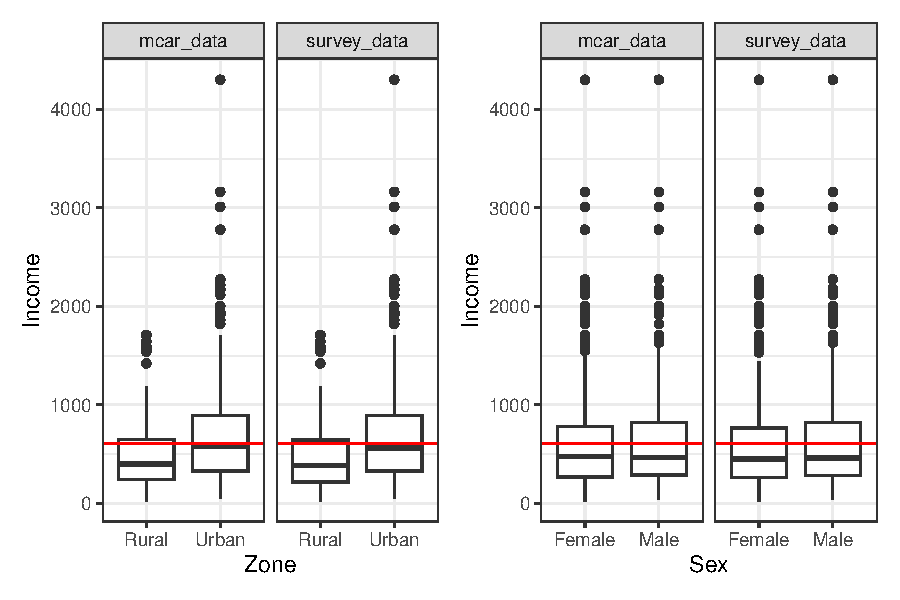
\includegraphics[width=0.7\linewidth,height=\textheight,keepaspectratio]{chapters/../figures/fig-ap3-mcar-boxplots-1.pdf}

}

\caption{\label{fig-ap3-mcar-boxplots}Distribución del ingreso por zona
y sexo con datos completos y bajo un patrón MCAR}

\end{figure}%

El siguiente código computacional muestra las densidades del ingreso
para la base completa (\texttt{survey\_data}) y la muestra con pérdida
MCAR (\texttt{mcar\_data}), en el total y por sexo
(figura~\ref{fig-ap3-mcar-income}). Las curvas prácticamente se
superponen, lo que indica pocos cambios en la distribución en esta
simulación. La línea roja representa la media del ingreso en la base
completa.

\begin{Shaded}
\begin{Highlighting}[]
\NormalTok{income\_density\_plot }\OtherTok{\textless{}{-}} \FunctionTok{ggplot}\NormalTok{(}
\NormalTok{  mcar\_plot\_data,}
  \FunctionTok{aes}\NormalTok{(}\AttributeTok{x =}\NormalTok{ Income, }\AttributeTok{fill =}\NormalTok{ data\_source)}
\NormalTok{) }\SpecialCharTok{+}
  \FunctionTok{geom\_density}\NormalTok{(}\AttributeTok{alpha =} \FloatTok{0.3}\NormalTok{) }\SpecialCharTok{+}
  \FunctionTok{theme\_bw}\NormalTok{() }\SpecialCharTok{+}
  \FunctionTok{theme}\NormalTok{(}\AttributeTok{legend.position =} \StringTok{"bottom"}\NormalTok{) }\SpecialCharTok{+}
  \FunctionTok{geom\_vline}\NormalTok{(}\AttributeTok{xintercept =} \FunctionTok{mean}\NormalTok{(survey\_data}\SpecialCharTok{$}\NormalTok{Income), }\AttributeTok{color =} \StringTok{"red"}\NormalTok{)}

\NormalTok{sex\_income\_density\_plot }\OtherTok{\textless{}{-}}\NormalTok{ income\_density\_plot }\SpecialCharTok{+}
  \FunctionTok{facet\_grid}\NormalTok{(. }\SpecialCharTok{\textasciitilde{}}\NormalTok{ Sex) }\SpecialCharTok{+}
  \FunctionTok{theme}\NormalTok{(}\AttributeTok{legend.position =} \StringTok{"none"}\NormalTok{)}

\NormalTok{income\_density\_plot }\SpecialCharTok{/}\NormalTok{ sex\_income\_density\_plot}
\end{Highlighting}
\end{Shaded}

\begin{figure}[H]

\centering{

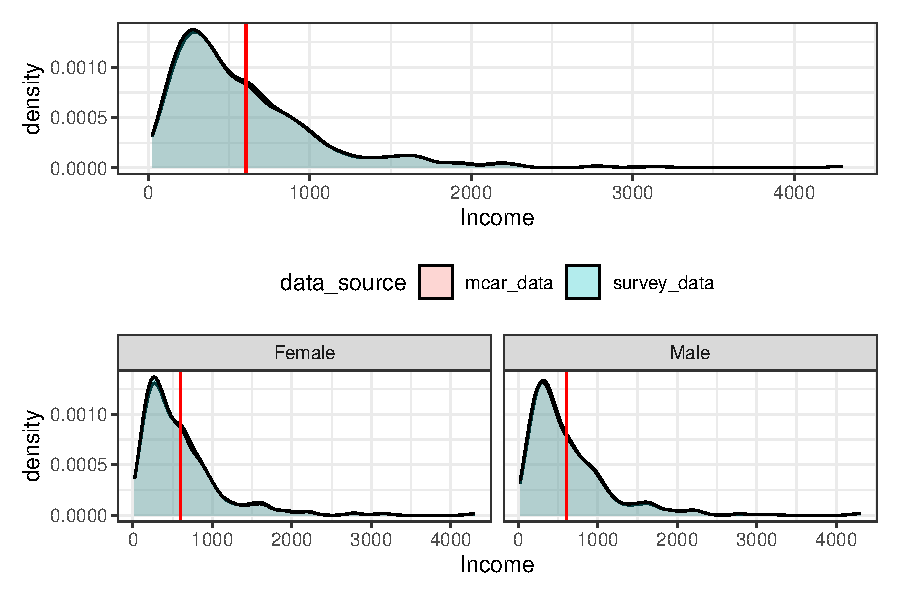
\includegraphics[width=0.7\linewidth,height=\textheight,keepaspectratio]{chapters/../figures/fig-ap3-mcar-income-1.pdf}

}

\caption{\label{fig-ap3-mcar-income}Distribución del ingreso, total y
por sexo, bajo un patrón MCAR}

\end{figure}%

El siguiente código computacional compara las densidades del gasto en la
base completa (\texttt{survey\_data}) y la muestra con pérdida MCAR
(\texttt{mcar\_data}), en el total y por sexo
(figura~\ref{fig-ap3-mcar-expenditure}). La superposición de las curvas
muestra que se conserva la forma de la distribución. La línea roja
indica la media del gasto en la base completa.

\begin{Shaded}
\begin{Highlighting}[]
\NormalTok{expenditure\_density\_plot }\OtherTok{\textless{}{-}} \FunctionTok{ggplot}\NormalTok{(}
\NormalTok{  mcar\_plot\_data,}
  \FunctionTok{aes}\NormalTok{(}\AttributeTok{x =}\NormalTok{ Expenditure, }\AttributeTok{fill =}\NormalTok{ data\_source)}
\NormalTok{) }\SpecialCharTok{+}
  \FunctionTok{geom\_density}\NormalTok{(}\AttributeTok{alpha =} \FloatTok{0.3}\NormalTok{) }\SpecialCharTok{+}
  \FunctionTok{theme\_bw}\NormalTok{() }\SpecialCharTok{+}
  \FunctionTok{theme}\NormalTok{(}\AttributeTok{legend.position =} \StringTok{"bottom"}\NormalTok{) }\SpecialCharTok{+}
  \FunctionTok{geom\_vline}\NormalTok{(}
    \AttributeTok{xintercept =} \FunctionTok{mean}\NormalTok{(survey\_data}\SpecialCharTok{$}\NormalTok{Expenditure),}
    \AttributeTok{color =} \StringTok{"red"}
\NormalTok{  )}

\NormalTok{sex\_expenditure\_density\_plot }\OtherTok{\textless{}{-}}\NormalTok{ expenditure\_density\_plot }\SpecialCharTok{+}
  \FunctionTok{facet\_grid}\NormalTok{(. }\SpecialCharTok{\textasciitilde{}}\NormalTok{ Sex) }\SpecialCharTok{+}
  \FunctionTok{theme}\NormalTok{(}\AttributeTok{legend.position =} \StringTok{"none"}\NormalTok{)}

\NormalTok{expenditure\_density\_plot }\SpecialCharTok{/}\NormalTok{ sex\_expenditure\_density\_plot}
\end{Highlighting}
\end{Shaded}

\begin{figure}[H]

\centering{

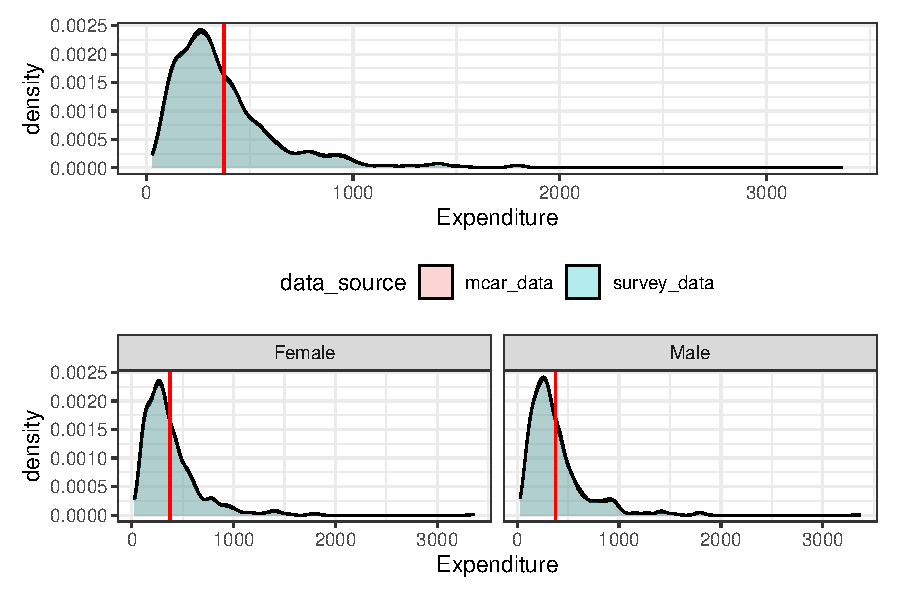
\includegraphics[width=0.7\linewidth,height=\textheight,keepaspectratio]{chapters/../figures/fig-ap3-mcar-expenditure-1.pdf}

}

\caption{\label{fig-ap3-mcar-expenditure}Distribución del gasto, total y
por sexo, bajo un patrón MCAR}

\end{figure}%

A continuación, se simula una pérdida de información al azar (MAR) que
depende de la zona y del sexo:

\begin{Shaded}
\begin{Highlighting}[]
\FunctionTok{set.seed}\NormalTok{(}\DecValTok{1234}\NormalTok{)}
\NormalTok{stratum\_id }\OtherTok{\textless{}{-}} \FunctionTok{paste0}\NormalTok{(survey\_data}\SpecialCharTok{$}\NormalTok{Zone, survey\_data}\SpecialCharTok{$}\NormalTok{Sex)}
\NormalTok{stratum\_sizes }\OtherTok{\textless{}{-}} \FunctionTok{table}\NormalTok{(stratum\_id)}
\NormalTok{stratum\_sizes}
\end{Highlighting}
\end{Shaded}

\begin{verbatim}
stratum_id
RuralFemale   RuralMale UrbanFemale   UrbanMale 
        481         428         531         439 
\end{verbatim}

\begin{Shaded}
\begin{Highlighting}[]
\NormalTok{sample\_indices }\OtherTok{\textless{}{-}} \FunctionTok{S.STSI}\NormalTok{(}
  \AttributeTok{S =}\NormalTok{ stratum\_id,}
  \AttributeTok{Nh =} \FunctionTok{as.numeric}\NormalTok{(stratum\_sizes),}
  \AttributeTok{nh =} \FunctionTok{c}\NormalTok{(}\DecValTok{20}\NormalTok{, }\DecValTok{380}\NormalTok{, }\DecValTok{20}\NormalTok{, }\DecValTok{280}\NormalTok{)}
\NormalTok{)}
\NormalTok{mar\_data }\OtherTok{\textless{}{-}}\NormalTok{ survey\_data[}\SpecialCharTok{{-}}\NormalTok{sample\_indices, ]}

\NormalTok{mar\_plot\_data }\OtherTok{\textless{}{-}} \FunctionTok{bind\_rows}\NormalTok{(}
  \FunctionTok{list}\NormalTok{(}\AttributeTok{mar\_data =}\NormalTok{ mar\_data, }\AttributeTok{survey\_data =}\NormalTok{ survey\_data),}
  \AttributeTok{.id =} \StringTok{"data\_source"}
\NormalTok{)}
\end{Highlighting}
\end{Shaded}

El código anterior utiliza el paquete \texttt{TeachingSampling} para
realizar un muestreo aleatorio en cada combinación de zona y sexo.
Primero, se fija la semilla en \texttt{1234} para que los resultados
sean reproducibles. Luego, se crea la variable \texttt{stratum\_id}, que
combina \texttt{Zone} y \texttt{Sex} mediante la función \texttt{paste0}
para definir los estratos. La función \texttt{table} muestra la
frecuencia de cada estrato. El muestreo estratificado se realiza con
\texttt{S.STSI}, cuyos argumentos son \texttt{S}, el vector de estratos;
\texttt{Nh}, el número de unidades en cada estrato (481, 428, 531, 439,
en el orden mostrado por \texttt{stratum\_sizes}); y \texttt{nh}, el
tamaño de muestra deseado en cada estrato (20, 380, 20 y 280).

El muestreo estratificado devuelve un vector con los índices de las
filas seleccionadas. Estas observaciones se excluyen de la base para
crear \texttt{mar\_data}. Por último, la función \texttt{bind\_rows} del
paquete \texttt{dplyr} reúne \texttt{survey\_data} y \texttt{mar\_data}
en \texttt{mar\_plot\_data}. La nueva variable \texttt{data\_source}
identifica la base de origen de cada observación.

El siguiente código computacional compara el gasto por zona y sexo entre
la base completa (\texttt{survey\_data}) y la muestra con pérdida MAR
(\texttt{mar\_data}) (figura~\ref{fig-ap3-mar-boxplots}). Las medianas
permanecen próximas, aunque cambian la dispersión y algunos valores
extremos, especialmente entre los hombres. La línea roja señala la media
del gasto en la base completa.

\begin{Shaded}
\begin{Highlighting}[]
\NormalTok{mar\_expenditure\_boxplot }\OtherTok{\textless{}{-}} \FunctionTok{ggplot}\NormalTok{(}
\NormalTok{  mar\_plot\_data,}
  \FunctionTok{aes}\NormalTok{(}\AttributeTok{x =}\NormalTok{ data\_source, }\AttributeTok{y =}\NormalTok{ Expenditure)}
\NormalTok{) }\SpecialCharTok{+}
  \FunctionTok{geom\_hline}\NormalTok{(}
    \AttributeTok{yintercept =} \FunctionTok{mean}\NormalTok{(survey\_data}\SpecialCharTok{$}\NormalTok{Expenditure),}
    \AttributeTok{color =} \StringTok{"red"}
\NormalTok{  ) }\SpecialCharTok{+}
  \FunctionTok{geom\_boxplot}\NormalTok{() }\SpecialCharTok{+}
  \FunctionTok{facet\_grid}\NormalTok{(Zone }\SpecialCharTok{\textasciitilde{}}\NormalTok{ Sex) }\SpecialCharTok{+}
  \FunctionTok{theme\_bw}\NormalTok{()}

\NormalTok{mar\_expenditure\_boxplot}
\end{Highlighting}
\end{Shaded}

\begin{figure}[H]

\centering{

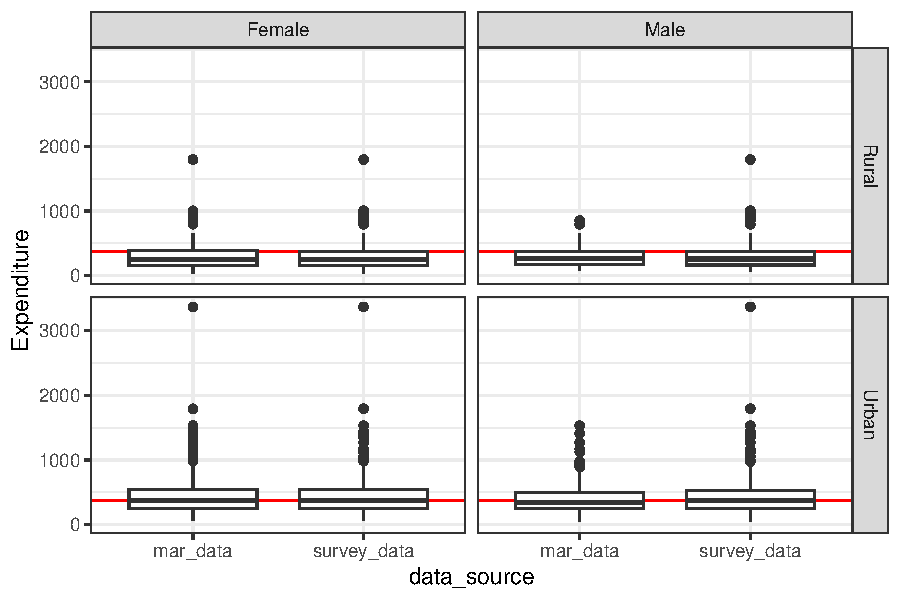
\includegraphics[width=0.7\linewidth,height=\textheight,keepaspectratio]{chapters/../figures/fig-ap3-mar-boxplots-1.pdf}

}

\caption{\label{fig-ap3-mar-boxplots}Distribución del gasto por zona y
sexo bajo un patrón MAR}

\end{figure}%

El siguiente código computacional compara las densidades del ingreso de
la base completa (\texttt{survey\_data}) y la muestra con pérdida MAR
(\texttt{mar\_data}) (figura~\ref{fig-ap3-mar-income}). Las diferencias
son pequeñas en el total y más visibles entre los hombres, lo que
muestra la utilidad de revisar las desagregaciones. La línea roja indica
la media del ingreso en la base completa.

\begin{Shaded}
\begin{Highlighting}[]
\NormalTok{income\_density\_plot }\OtherTok{\textless{}{-}} \FunctionTok{ggplot}\NormalTok{(}
\NormalTok{  mar\_plot\_data,}
  \FunctionTok{aes}\NormalTok{(}\AttributeTok{x =}\NormalTok{ Income, }\AttributeTok{fill =}\NormalTok{ data\_source)}
\NormalTok{) }\SpecialCharTok{+}
  \FunctionTok{geom\_density}\NormalTok{(}\AttributeTok{alpha =} \FloatTok{0.3}\NormalTok{) }\SpecialCharTok{+}
  \FunctionTok{theme\_bw}\NormalTok{() }\SpecialCharTok{+}
  \FunctionTok{theme}\NormalTok{(}\AttributeTok{legend.position =} \StringTok{"bottom"}\NormalTok{) }\SpecialCharTok{+}
  \FunctionTok{geom\_vline}\NormalTok{(}\AttributeTok{xintercept =} \FunctionTok{mean}\NormalTok{(survey\_data}\SpecialCharTok{$}\NormalTok{Income), }\AttributeTok{color =} \StringTok{"red"}\NormalTok{)}

\NormalTok{sex\_income\_density\_plot }\OtherTok{\textless{}{-}}\NormalTok{ income\_density\_plot }\SpecialCharTok{+}
  \FunctionTok{facet\_grid}\NormalTok{(. }\SpecialCharTok{\textasciitilde{}}\NormalTok{ Sex) }\SpecialCharTok{+}
  \FunctionTok{theme}\NormalTok{(}\AttributeTok{legend.position =} \StringTok{"none"}\NormalTok{)}

\NormalTok{income\_density\_plot }\SpecialCharTok{/}\NormalTok{ sex\_income\_density\_plot}
\end{Highlighting}
\end{Shaded}

\begin{figure}[H]

\centering{

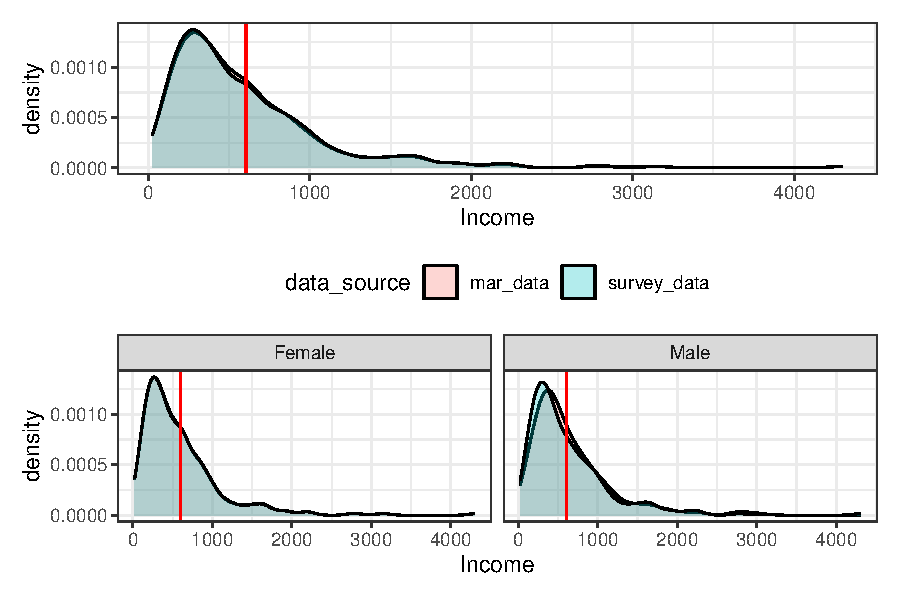
\includegraphics[width=0.7\linewidth,height=\textheight,keepaspectratio]{chapters/../figures/fig-ap3-mar-income-1.pdf}

}

\caption{\label{fig-ap3-mar-income}Distribución del ingreso, total y por
sexo, bajo un patrón MAR}

\end{figure}%

El siguiente código computacional muestra las densidades del gasto en la
base completa (\texttt{survey\_data}) y la muestra con pérdida MAR
(\texttt{mar\_data}), en el total y por sexo
(figura~\ref{fig-ap3-mar-expenditure}). Las curvas son próximas entre
las mujeres y presentan diferencias más visibles entre los hombres. La
línea roja representa la media del gasto en la base completa.

\begin{Shaded}
\begin{Highlighting}[]
\NormalTok{expenditure\_density\_plot }\OtherTok{\textless{}{-}} \FunctionTok{ggplot}\NormalTok{(}
\NormalTok{  mar\_plot\_data,}
  \FunctionTok{aes}\NormalTok{(}\AttributeTok{x =}\NormalTok{ Expenditure, }\AttributeTok{fill =}\NormalTok{ data\_source)}
\NormalTok{) }\SpecialCharTok{+}
  \FunctionTok{geom\_density}\NormalTok{(}\AttributeTok{alpha =} \FloatTok{0.3}\NormalTok{) }\SpecialCharTok{+}
  \FunctionTok{theme\_bw}\NormalTok{() }\SpecialCharTok{+}
  \FunctionTok{theme}\NormalTok{(}\AttributeTok{legend.position =} \StringTok{"bottom"}\NormalTok{) }\SpecialCharTok{+}
  \FunctionTok{geom\_vline}\NormalTok{(}
    \AttributeTok{xintercept =} \FunctionTok{mean}\NormalTok{(survey\_data}\SpecialCharTok{$}\NormalTok{Expenditure),}
    \AttributeTok{color =} \StringTok{"red"}
\NormalTok{  )}

\NormalTok{sex\_expenditure\_density\_plot }\OtherTok{\textless{}{-}}\NormalTok{ expenditure\_density\_plot }\SpecialCharTok{+}
  \FunctionTok{facet\_grid}\NormalTok{(. }\SpecialCharTok{\textasciitilde{}}\NormalTok{ Sex) }\SpecialCharTok{+}
  \FunctionTok{theme}\NormalTok{(}\AttributeTok{legend.position =} \StringTok{"none"}\NormalTok{)}

\NormalTok{expenditure\_density\_plot }\SpecialCharTok{/}\NormalTok{ sex\_expenditure\_density\_plot}
\end{Highlighting}
\end{Shaded}

\begin{figure}[H]

\centering{

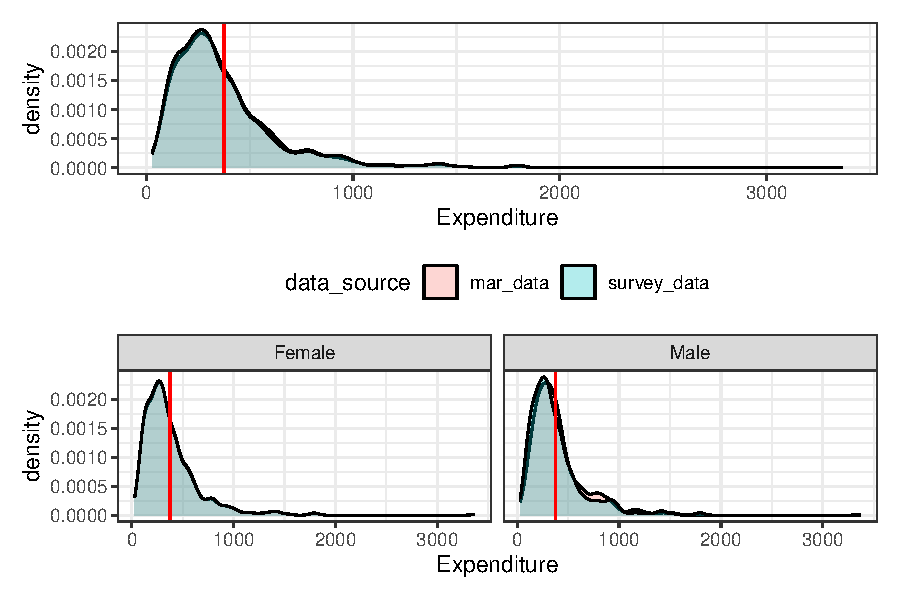
\includegraphics[width=0.7\linewidth,height=\textheight,keepaspectratio]{chapters/../figures/fig-ap3-mar-expenditure-1.pdf}

}

\caption{\label{fig-ap3-mar-expenditure}Distribución del gasto, total y
por sexo, bajo un patrón MAR}

\end{figure}%

Por último, se simula una pérdida de información no al azar (MNAR). Como
se explicó al inicio del anexo, en este mecanismo la probabilidad de que
un dato falte está relacionada con su propio valor. Esta dependencia
puede introducir un sesgo apreciable en la inferencia y el análisis
estadístico de las encuestas de hogares, por lo que el tratamiento de
los datos faltantes requiere especial atención. El siguiente código
computacional crea \texttt{mnar\_data} conservando las 1.300
observaciones con menor ingreso y la combina con la base completa para
comparar ambas distribuciones.

\begin{Shaded}
\begin{Highlighting}[]
\NormalTok{mnar\_data }\OtherTok{\textless{}{-}}\NormalTok{ survey\_data }\SpecialCharTok{\%\textgreater{}\%}
  \FunctionTok{arrange}\NormalTok{(Income) }\SpecialCharTok{\%\textgreater{}\%}
  \FunctionTok{slice}\NormalTok{(}\DecValTok{1}\SpecialCharTok{:}\DecValTok{1300}\NormalTok{L)}

\NormalTok{mnar\_plot\_data }\OtherTok{\textless{}{-}} \FunctionTok{bind\_rows}\NormalTok{(}
  \FunctionTok{list}\NormalTok{(}\AttributeTok{mnar\_data =}\NormalTok{ mnar\_data, }\AttributeTok{survey\_data =}\NormalTok{ survey\_data),}
  \AttributeTok{.id =} \StringTok{"data\_source"}
\NormalTok{)}
\end{Highlighting}
\end{Shaded}

El código anterior conserva en \texttt{mnar\_data} las 1.300
observaciones con menores ingresos y las reúne con la base completa en
\texttt{mnar\_plot\_data}. La figura~\ref{fig-ap3-mnar-income}, obtenida
con el siguiente código computacional, muestra cómo esta selección
elimina la cola de ingresos altos y desplaza la distribución hacia
valores menores. La media de los casos conservados, en azul, queda por
debajo de la media de la base completa, en rojo.

\begin{Shaded}
\begin{Highlighting}[]
\NormalTok{mnar\_income\_density\_plot }\OtherTok{\textless{}{-}} \FunctionTok{ggplot}\NormalTok{(}
\NormalTok{  mnar\_plot\_data,}
  \FunctionTok{aes}\NormalTok{(}\AttributeTok{x =}\NormalTok{ Income, }\AttributeTok{fill =}\NormalTok{ data\_source)}
\NormalTok{) }\SpecialCharTok{+}
  \FunctionTok{geom\_density}\NormalTok{(}\AttributeTok{alpha =} \FloatTok{0.2}\NormalTok{) }\SpecialCharTok{+}
  \FunctionTok{theme\_bw}\NormalTok{() }\SpecialCharTok{+}
  \FunctionTok{theme}\NormalTok{(}\AttributeTok{legend.position =} \StringTok{"bottom"}\NormalTok{) }\SpecialCharTok{+}
  \FunctionTok{geom\_vline}\NormalTok{(}\AttributeTok{xintercept =} \FunctionTok{mean}\NormalTok{(survey\_data}\SpecialCharTok{$}\NormalTok{Income), }\AttributeTok{color =} \StringTok{"red"}\NormalTok{) }\SpecialCharTok{+}
  \FunctionTok{geom\_vline}\NormalTok{(}\AttributeTok{xintercept =} \FunctionTok{mean}\NormalTok{(mnar\_data}\SpecialCharTok{$}\NormalTok{Income), }\AttributeTok{color =} \StringTok{"blue"}\NormalTok{)}

\NormalTok{mnar\_income\_density\_plot}
\end{Highlighting}
\end{Shaded}

\begin{figure}[H]

\centering{

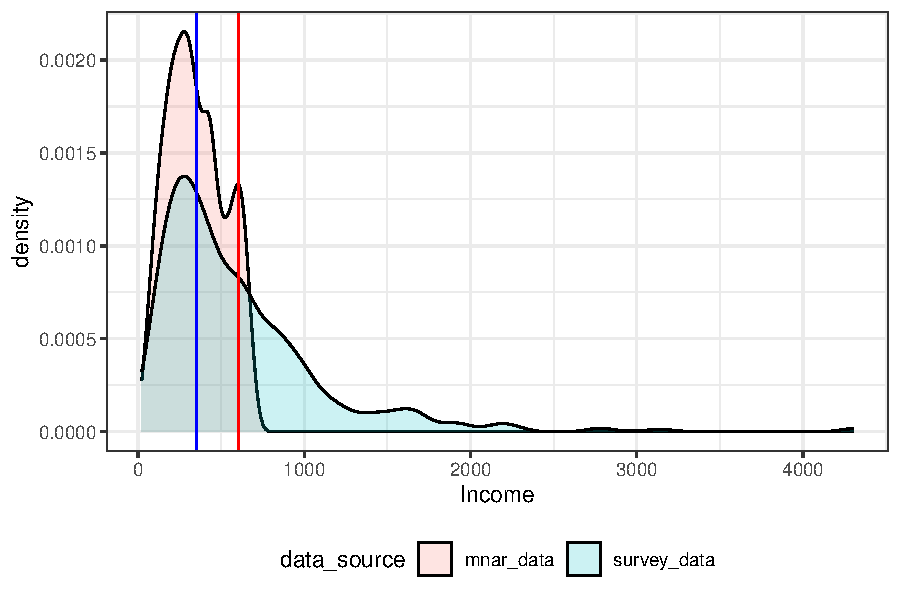
\includegraphics[width=0.7\linewidth,height=\textheight,keepaspectratio]{chapters/../figures/fig-ap3-mnar-income-1.pdf}

}

\caption{\label{fig-ap3-mnar-income}Distribución del ingreso bajo un
patrón MNAR}

\end{figure}%

El siguiente código computacional compara la distribución del gasto en
la base completa (\texttt{survey\_data}) y entre los casos conservados
bajo MNAR (\texttt{mnar\_data}) (figura~\ref{fig-ap3-mnar-expenditure}).
La selección por ingreso también reduce la presencia de gastos altos. La
línea azul señala la media del gasto de los casos conservados y la roja,
la media de la base completa.

\begin{Shaded}
\begin{Highlighting}[]
\NormalTok{mnar\_expenditure\_density\_plot }\OtherTok{\textless{}{-}} \FunctionTok{ggplot}\NormalTok{(}
\NormalTok{  mnar\_plot\_data,}
  \FunctionTok{aes}\NormalTok{(}\AttributeTok{x =}\NormalTok{ Expenditure, }\AttributeTok{fill =}\NormalTok{ data\_source)}
\NormalTok{) }\SpecialCharTok{+}
  \FunctionTok{geom\_density}\NormalTok{(}\AttributeTok{alpha =} \FloatTok{0.2}\NormalTok{) }\SpecialCharTok{+}
  \FunctionTok{theme\_bw}\NormalTok{() }\SpecialCharTok{+}
  \FunctionTok{theme}\NormalTok{(}\AttributeTok{legend.position =} \StringTok{"bottom"}\NormalTok{) }\SpecialCharTok{+}
  \FunctionTok{geom\_vline}\NormalTok{(}
    \AttributeTok{xintercept =} \FunctionTok{mean}\NormalTok{(survey\_data}\SpecialCharTok{$}\NormalTok{Expenditure),}
    \AttributeTok{color =} \StringTok{"red"}
\NormalTok{  ) }\SpecialCharTok{+}
  \FunctionTok{geom\_vline}\NormalTok{(}
    \AttributeTok{xintercept =} \FunctionTok{mean}\NormalTok{(mnar\_data}\SpecialCharTok{$}\NormalTok{Expenditure),}
    \AttributeTok{color =} \StringTok{"blue"}
\NormalTok{  )}

\NormalTok{mnar\_expenditure\_density\_plot}
\end{Highlighting}
\end{Shaded}

\begin{figure}[H]

\centering{

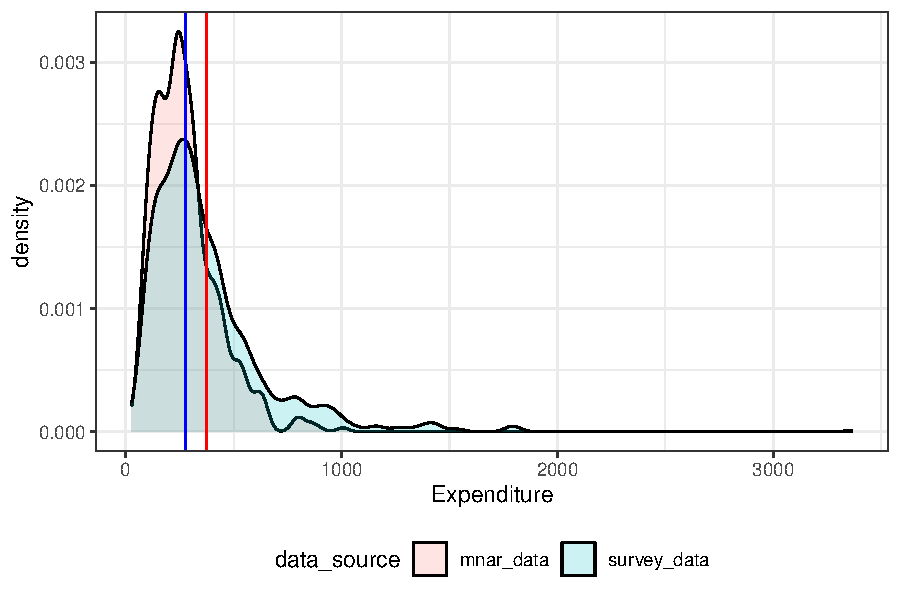
\includegraphics[width=0.7\linewidth,height=\textheight,keepaspectratio]{chapters/../figures/fig-ap3-mnar-expenditure-1.pdf}

}

\caption{\label{fig-ap3-mnar-expenditure}Distribución del gasto bajo un
patrón MNAR}

\end{figure}%

El siguiente código computacional compara el ingreso por zona y sexo en
la base completa (\texttt{survey\_data}) y entre los casos conservados
bajo MNAR (\texttt{mnar\_data}) (figura~\ref{fig-ap3-mnar-boxplots}). La
eliminación de ingresos altos reduce las medianas y la dispersión, con
cambios más marcados en la zona urbana. La línea roja indica la media
del ingreso en la base completa.

\begin{Shaded}
\begin{Highlighting}[]
\NormalTok{mnar\_income\_boxplot }\OtherTok{\textless{}{-}} \FunctionTok{ggplot}\NormalTok{(}
\NormalTok{  mnar\_plot\_data,}
  \FunctionTok{aes}\NormalTok{(}\AttributeTok{x =}\NormalTok{ data\_source, }\AttributeTok{y =}\NormalTok{ Income)}
\NormalTok{) }\SpecialCharTok{+}
  \FunctionTok{geom\_hline}\NormalTok{(}\AttributeTok{yintercept =} \FunctionTok{mean}\NormalTok{(survey\_data}\SpecialCharTok{$}\NormalTok{Income), }\AttributeTok{color =} \StringTok{"red"}\NormalTok{) }\SpecialCharTok{+}
  \FunctionTok{geom\_boxplot}\NormalTok{() }\SpecialCharTok{+}
  \FunctionTok{facet\_grid}\NormalTok{(Zone }\SpecialCharTok{\textasciitilde{}}\NormalTok{ Sex) }\SpecialCharTok{+}
  \FunctionTok{theme\_bw}\NormalTok{()}

\NormalTok{mnar\_income\_boxplot}
\end{Highlighting}
\end{Shaded}

\begin{figure}[H]

\centering{

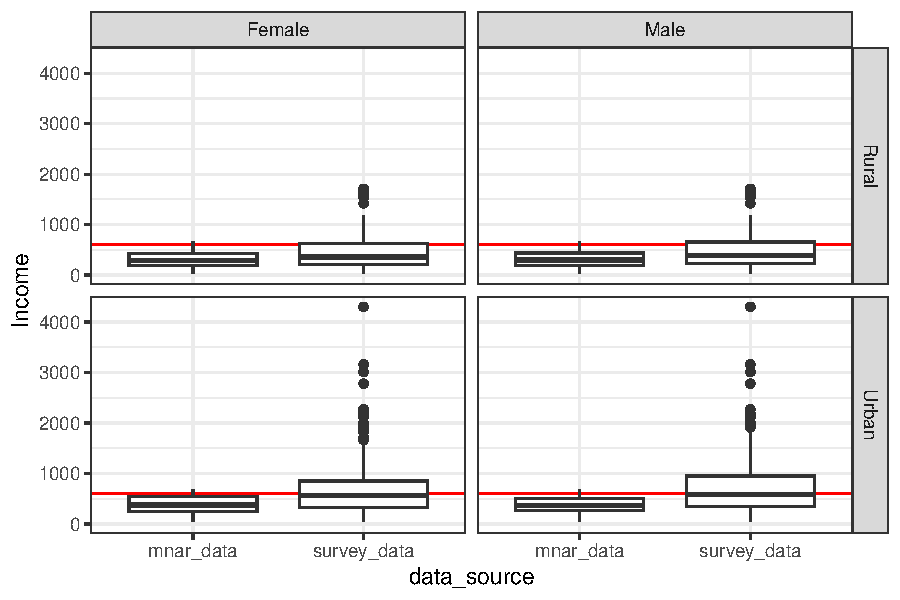
\includegraphics[width=0.7\linewidth,height=\textheight,keepaspectratio]{chapters/../figures/fig-ap3-mnar-boxplots-1.pdf}

}

\caption{\label{fig-ap3-mnar-boxplots}Distribución del ingreso por zona
y sexo bajo un patrón MNAR}

\end{figure}%

\section{Algunos métodos de
imputación}\label{algunos-muxe9todos-de-imputaciuxf3n}

La sección anterior mostró cómo los mecanismos MCAR, MAR y MNAR pueden
afectar la distribución de los datos observados. A partir de ese
diagnóstico, esta sección presenta distintos métodos para reemplazar los
valores faltantes utilizando la información disponible. Mediante
ejemplos en \texttt{R}, se comparan los ingresos originales con los
obtenidos por imputación, prestando atención tanto a su media como a su
dispersión y distribución. El recorrido comienza con métodos de
imputación simple y concluye con la imputación múltiple.

\subsection{Imputación por la media no
condicional}\label{imputaciuxf3n-por-la-media-no-condicional}

La imputación por la media no condicional consiste en reemplazar los
valores faltantes con la media aritmética de los valores observados de
la variable, sin considerar otras variables. La media se calcula a
partir de todos los valores disponibles, independientemente de las
características de las observaciones.

Para ilustrar el tratamiento de los datos faltantes bajo un mecanismo
MCAR, se construye la siguiente base de datos:

\begin{Shaded}
\begin{Highlighting}[]
\NormalTok{survey\_data }\OtherTok{\textless{}{-}} \FunctionTok{full\_join}\NormalTok{(}
\NormalTok{  survey\_data,}
\NormalTok{  mcar\_data }\SpecialCharTok{\%\textgreater{}\%} \FunctionTok{transmute}\NormalTok{(}
\NormalTok{    HHID,}
\NormalTok{    PersonID,}
    \AttributeTok{income\_missing =}\NormalTok{ Income,}
    \AttributeTok{employment\_missing =}\NormalTok{ Employment}
\NormalTok{  ),}
  \AttributeTok{by =} \FunctionTok{c}\NormalTok{(}\StringTok{"HHID"}\NormalTok{, }\StringTok{"PersonID"}\NormalTok{)}
\NormalTok{)}
\end{Highlighting}
\end{Shaded}

El código anterior utiliza la función \texttt{full\_join} del paquete
\texttt{dplyr} para combinar las dos bases de datos. Esta unión conserva
todas las filas de ambas bases, combina las que tienen claves
coincidentes y asigna valores faltantes donde no hay correspondencia.
Para conocer el porcentaje de valores faltantes, se ejecuta el siguiente
código:

\begin{Shaded}
\begin{Highlighting}[]
\NormalTok{survey\_data }\SpecialCharTok{\%\textgreater{}\%}
  \FunctionTok{group\_by}\NormalTok{(Zone) }\SpecialCharTok{\%\textgreater{}\%}
  \FunctionTok{summarise}\NormalTok{(}
    \AttributeTok{missing\_proportion =} \FunctionTok{sum}\NormalTok{(}\FunctionTok{is.na}\NormalTok{(income\_missing) }\SpecialCharTok{/} \FunctionTok{n}\NormalTok{())}
\NormalTok{  )}
\end{Highlighting}
\end{Shaded}

\begin{verbatim}
# A tibble: 2 x 2
  Zone  missing_proportion
  <chr>              <dbl>
1 Rural              0.208
2 Urban              0.193
\end{verbatim}

\begin{Shaded}
\begin{Highlighting}[]
\NormalTok{survey\_data }\SpecialCharTok{\%\textgreater{}\%}
  \FunctionTok{group\_by}\NormalTok{(Sex) }\SpecialCharTok{\%\textgreater{}\%}
  \FunctionTok{summarise}\NormalTok{(}
    \AttributeTok{missing\_proportion =} \FunctionTok{sum}\NormalTok{(}\FunctionTok{is.na}\NormalTok{(income\_missing) }\SpecialCharTok{/} \FunctionTok{n}\NormalTok{())}
\NormalTok{  )}
\end{Highlighting}
\end{Shaded}

\begin{verbatim}
# A tibble: 2 x 2
  Sex    missing_proportion
  <chr>               <dbl>
1 Female              0.184
2 Male                0.219
\end{verbatim}

La imputación por la media no condicional es un método simple y rápido.
Puede resultar útil cuando la distribución de la variable no es muy
asimétrica o cuando hay pocos valores faltantes en relación con el
tamaño de la muestra. Sin embargo, presenta limitaciones cuando existen
sesgos o patrones en los datos faltantes, o cuando las variables están
muy correlacionadas. Aunque conserva la media de los valores observados,
modifica la variabilidad y los percentiles, y puede afectar el sesgo. El
método se aplica de la siguiente manera:

\begin{Shaded}
\begin{Highlighting}[]
\NormalTok{observed\_income\_mean }\OtherTok{\textless{}{-}} \FunctionTok{mean}\NormalTok{(survey\_data}\SpecialCharTok{$}\NormalTok{income\_missing, }\AttributeTok{na.rm =} \ConstantTok{TRUE}\NormalTok{)}
\NormalTok{survey\_data }\OtherTok{\textless{}{-}}\NormalTok{ survey\_data }\SpecialCharTok{\%\textgreater{}\%}
  \FunctionTok{mutate}\NormalTok{(}
    \AttributeTok{income\_imputed =} \FunctionTok{ifelse}\NormalTok{(}
      \FunctionTok{is.na}\NormalTok{(income\_missing),}
\NormalTok{      observed\_income\_mean,}
\NormalTok{      income\_missing}
\NormalTok{    )}
\NormalTok{  )}

\FunctionTok{sum}\NormalTok{(}\FunctionTok{is.na}\NormalTok{(survey\_data}\SpecialCharTok{$}\NormalTok{income\_imputed))}
\end{Highlighting}
\end{Shaded}

\begin{verbatim}
[1] 0
\end{verbatim}

El código anterior calcula la media de los valores observados de
\texttt{income\_missing} y la almacena en
\texttt{observed\_income\_mean}. Luego, reemplaza los valores faltantes
con esa media y guarda el resultado en \texttt{income\_imputed}. La
última línea cuenta los valores faltantes de esta nueva columna de
\texttt{survey\_data} y confirma que no quedan datos sin imputar.

El siguiente código computacional compara el ingreso original
(\texttt{Income}) con el completado mediante la media no condicional
(\texttt{income\_imputed}) (figura~\ref{fig-ap3-mean-non-conditional}).
La imputación produce una concentración artificial alrededor de la
media, visible como un pico pronunciado. Las líneas roja y azul
representan las medias original e imputada, respectivamente; su cercanía
no implica que las distribuciones sean iguales.

\begin{Shaded}
\begin{Highlighting}[]
\NormalTok{mean\_plot\_data }\OtherTok{\textless{}{-}}\NormalTok{ survey\_data }\SpecialCharTok{\%\textgreater{}\%}
\NormalTok{  dplyr}\SpecialCharTok{::}\FunctionTok{select}\NormalTok{(Zone, Sex, Income, income\_imputed) }\SpecialCharTok{\%\textgreater{}\%}
\NormalTok{  tidyr}\SpecialCharTok{::}\FunctionTok{gather}\NormalTok{(data\_source, income\_value, }\SpecialCharTok{{-}}\NormalTok{Zone, }\SpecialCharTok{{-}}\NormalTok{Sex)}

\NormalTok{mean\_density\_plot }\OtherTok{\textless{}{-}} \FunctionTok{ggplot}\NormalTok{(}
\NormalTok{  mean\_plot\_data,}
  \FunctionTok{aes}\NormalTok{(}\AttributeTok{x =}\NormalTok{ income\_value, }\AttributeTok{fill =}\NormalTok{ data\_source)}
\NormalTok{) }\SpecialCharTok{+}
  \FunctionTok{geom\_density}\NormalTok{(}\AttributeTok{alpha =} \FloatTok{0.2}\NormalTok{) }\SpecialCharTok{+}
  \FunctionTok{theme\_bw}\NormalTok{() }\SpecialCharTok{+}
  \FunctionTok{theme}\NormalTok{(}\AttributeTok{legend.position =} \StringTok{"bottom"}\NormalTok{) }\SpecialCharTok{+}
  \FunctionTok{geom\_vline}\NormalTok{(}\AttributeTok{xintercept =} \FunctionTok{mean}\NormalTok{(survey\_data}\SpecialCharTok{$}\NormalTok{Income), }\AttributeTok{color =} \StringTok{"red"}\NormalTok{) }\SpecialCharTok{+}
  \FunctionTok{geom\_vline}\NormalTok{(}
    \AttributeTok{xintercept =} \FunctionTok{mean}\NormalTok{(survey\_data}\SpecialCharTok{$}\NormalTok{income\_imputed),}
    \AttributeTok{color =} \StringTok{"blue"}
\NormalTok{  )}

\NormalTok{mean\_density\_plot}
\end{Highlighting}
\end{Shaded}

\begin{figure}[H]

\centering{

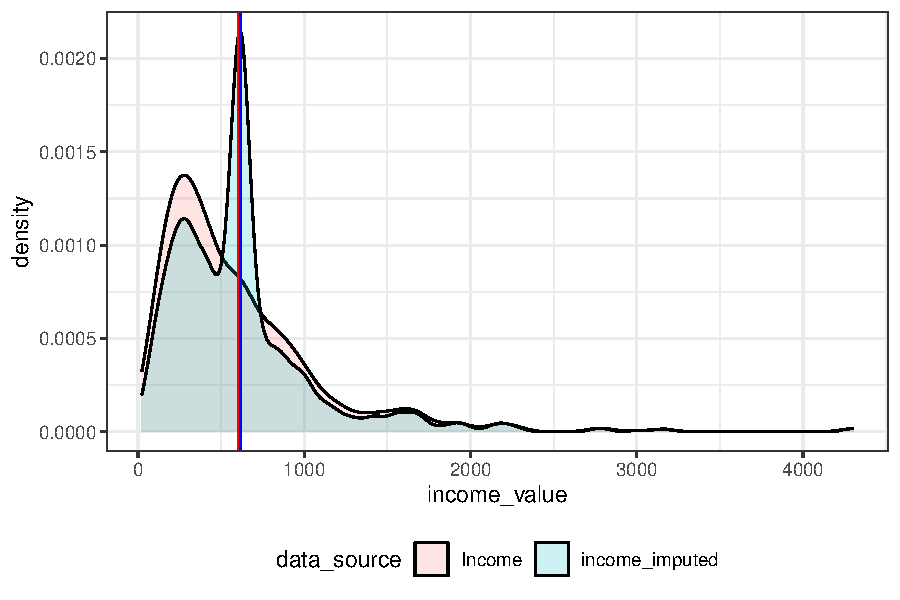
\includegraphics[width=0.7\linewidth,height=\textheight,keepaspectratio]{chapters/../figures/fig-ap3-mean-non-conditional-1.pdf}

}

\caption{\label{fig-ap3-mean-non-conditional}Distribución del ingreso
original e imputado por la media no condicional}

\end{figure}%

El siguiente código computacional compara el ingreso original
(\texttt{Income}) y el completado por la media no condicional
(\texttt{income\_imputed}) dentro de cada combinación de zona y sexo
(figura~\ref{fig-ap3-mean-non-conditional-groups}). Las cajas muestran
cambios en la mediana y la dispersión al asignar un mismo valor a todos
los datos faltantes. La línea roja señala la media del ingreso original.

\begin{Shaded}
\begin{Highlighting}[]
\NormalTok{mean\_boxplot }\OtherTok{\textless{}{-}} \FunctionTok{ggplot}\NormalTok{(}
\NormalTok{  mean\_plot\_data,}
  \FunctionTok{aes}\NormalTok{(}\AttributeTok{x =}\NormalTok{ data\_source, }\AttributeTok{y =}\NormalTok{ income\_value)}
\NormalTok{) }\SpecialCharTok{+}
  \FunctionTok{geom\_hline}\NormalTok{(}\AttributeTok{yintercept =} \FunctionTok{mean}\NormalTok{(survey\_data}\SpecialCharTok{$}\NormalTok{Income), }\AttributeTok{color =} \StringTok{"red"}\NormalTok{) }\SpecialCharTok{+}
  \FunctionTok{geom\_boxplot}\NormalTok{() }\SpecialCharTok{+}
  \FunctionTok{facet\_grid}\NormalTok{(Zone }\SpecialCharTok{\textasciitilde{}}\NormalTok{ Sex) }\SpecialCharTok{+}
  \FunctionTok{theme\_bw}\NormalTok{()}

\NormalTok{mean\_boxplot}
\end{Highlighting}
\end{Shaded}

\begin{figure}[H]

\centering{

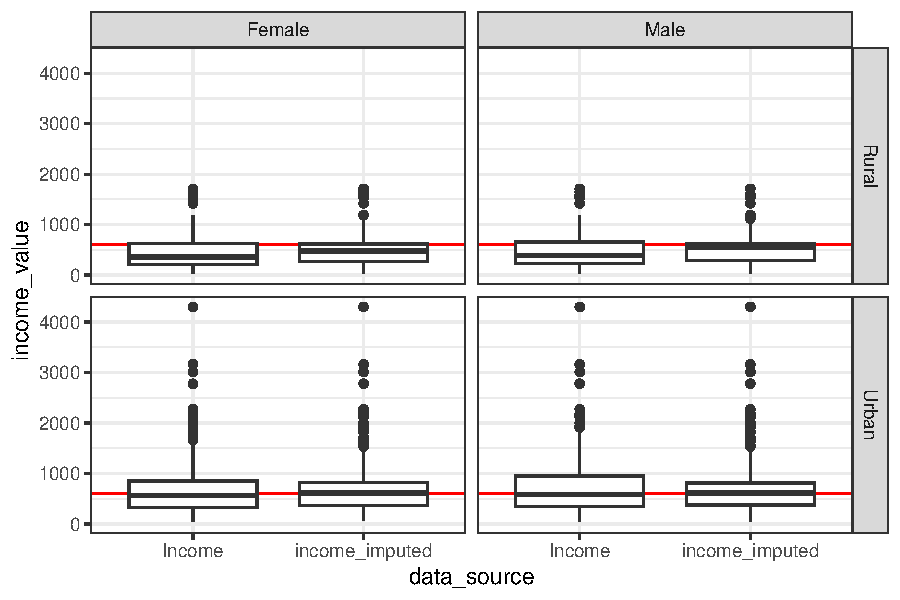
\includegraphics[width=0.7\linewidth,height=\textheight,keepaspectratio]{chapters/../figures/fig-ap3-mean-non-conditional-groups-1.pdf}

}

\caption{\label{fig-ap3-mean-non-conditional-groups}Ingreso original e
imputado por la media no condicional, por zona y sexo}

\end{figure}%

\subsection{Imputación por la media
condicional}\label{imputaciuxf3n-por-la-media-condicional}

La imputación por la media condicional reemplaza los valores faltantes
de una variable numérica con las medias calculadas en grupos de
observaciones que comparten características. A diferencia de la media no
condicional, este método considera otras variables, ya que la media de
la variable de interés puede cambiar según sus valores. Puede ofrecer
mayor precisión cuando las variables están correlacionadas o cuando
existen patrones de ausencia de respuesta asociados con las variables de
agrupación.

En el siguiente ejemplo, se calculan las medias por estrato para imputar
los ingresos faltantes, bajo el supuesto de que existe una relación
entre el estrato y el ingreso de los hogares:

\begin{Shaded}
\begin{Highlighting}[]
\NormalTok{survey\_data }\OtherTok{\textless{}{-}}\NormalTok{ survey\_data }\SpecialCharTok{\%\textgreater{}\%}
  \FunctionTok{group\_by}\NormalTok{(Stratum) }\SpecialCharTok{\%\textgreater{}\%}
  \FunctionTok{mutate}\NormalTok{(}
    \AttributeTok{income\_imputed =} \FunctionTok{ifelse}\NormalTok{(}
      \FunctionTok{is.na}\NormalTok{(income\_missing),}
      \FunctionTok{mean}\NormalTok{(income\_missing, }\AttributeTok{na.rm =} \ConstantTok{TRUE}\NormalTok{),}
\NormalTok{      income\_missing}
\NormalTok{    )}
\NormalTok{  ) }\SpecialCharTok{\%\textgreater{}\%}
  \FunctionTok{data.frame}\NormalTok{()}

\FunctionTok{sum}\NormalTok{(}\FunctionTok{is.na}\NormalTok{(survey\_data}\SpecialCharTok{$}\NormalTok{income\_imputed))}
\end{Highlighting}
\end{Shaded}

\begin{verbatim}
[1] 0
\end{verbatim}

\begin{Shaded}
\begin{Highlighting}[]
\NormalTok{survey\_data }\OtherTok{\textless{}{-}}\NormalTok{ survey\_data }\SpecialCharTok{\%\textgreater{}\%}
  \FunctionTok{mutate}\NormalTok{(}
    \AttributeTok{income\_imputed =} \FunctionTok{ifelse}\NormalTok{(}
      \FunctionTok{is.na}\NormalTok{(income\_imputed),}
\NormalTok{      observed\_income\_mean,}
\NormalTok{      income\_imputed}
\NormalTok{    )}
\NormalTok{  )}

\FunctionTok{sum}\NormalTok{(}\FunctionTok{is.na}\NormalTok{(survey\_data}\SpecialCharTok{$}\NormalTok{income\_imputed))}
\end{Highlighting}
\end{Shaded}

\begin{verbatim}
[1] 0
\end{verbatim}

El código anterior utiliza \texttt{group\_by} para agrupar las
observaciones de \texttt{survey\_data} por \texttt{Stratum}. Los valores
faltantes de \texttt{income\_missing} se reemplazan con la media de los
ingresos observados en el estrato correspondiente, mientras que los
valores observados se conservan. El resultado se almacena en
\texttt{income\_imputed}. A continuación, se calculan las medias y las
desviaciones estándar de los ingresos originales y de los completados
por imputación para comparar el efecto del método:

\begin{Shaded}
\begin{Highlighting}[]
\NormalTok{survey\_data }\SpecialCharTok{\%\textgreater{}\%}
  \FunctionTok{summarise}\NormalTok{(}
    \AttributeTok{income\_mean =} \FunctionTok{mean}\NormalTok{(Income),}
    \AttributeTok{income\_sd =} \FunctionTok{sd}\NormalTok{(Income),}
    \AttributeTok{imputed\_income\_mean =} \FunctionTok{mean}\NormalTok{(income\_imputed),}
    \AttributeTok{imputed\_income\_sd =} \FunctionTok{sd}\NormalTok{(income\_imputed)}
\NormalTok{  )}
\end{Highlighting}
\end{Shaded}

\begin{verbatim}
  income_mean income_sd imputed_income_mean imputed_income_sd
1         604       513                 612               489
\end{verbatim}

En este ejemplo, el sesgo relativo de la media del ingreso es de 1,21
\%, y el de la desviación estándar es de -4,75 \%. Al desagregar los
resultados de la imputación por zona, se obtiene lo siguiente:

\begin{Shaded}
\begin{Highlighting}[]
\NormalTok{survey\_data }\SpecialCharTok{\%\textgreater{}\%}
  \FunctionTok{group\_by}\NormalTok{(Zone) }\SpecialCharTok{\%\textgreater{}\%}
  \FunctionTok{summarise}\NormalTok{(}
    \AttributeTok{income\_mean =} \FunctionTok{mean}\NormalTok{(Income),}
    \AttributeTok{income\_sd =} \FunctionTok{sd}\NormalTok{(Income),}
    \AttributeTok{imputed\_income\_mean =} \FunctionTok{mean}\NormalTok{(income\_imputed),}
    \AttributeTok{imputed\_income\_sd =} \FunctionTok{sd}\NormalTok{(income\_imputed)}
\NormalTok{  )}
\end{Highlighting}
\end{Shaded}

\begin{verbatim}
# A tibble: 2 x 5
  Zone  income_mean income_sd imputed_income_mean imputed_income_sd
  <chr>       <dbl>     <dbl>               <dbl>             <dbl>
1 Rural        469.      337.                478.              306.
2 Urban        731.      609.                737.              586.
\end{verbatim}

Los sesgos relativos de la media del ingreso son del 1,87 \% en la zona
rural y del 0,81 \% en la urbana. En ambos casos, las medias obtenidas
tras la imputación son próximas a las originales.

El siguiente código computacional compara las densidades del ingreso
original (\texttt{Income}) y del completado con medias por estrato
(\texttt{income\_imputed}) (figura~\ref{fig-ap3-mean-conditional}). La
curva imputada se aproxima a la original, aunque conserva diferencias en
el tramo central. Las líneas roja y azul señalan las medias original e
imputada, respectivamente.

\begin{Shaded}
\begin{Highlighting}[]
\NormalTok{conditional\_mean\_plot\_data }\OtherTok{\textless{}{-}}\NormalTok{ survey\_data }\SpecialCharTok{\%\textgreater{}\%}
\NormalTok{  dplyr}\SpecialCharTok{::}\FunctionTok{select}\NormalTok{(Zone, Sex, Income, income\_imputed) }\SpecialCharTok{\%\textgreater{}\%}
\NormalTok{  tidyr}\SpecialCharTok{::}\FunctionTok{gather}\NormalTok{(data\_source, income\_value, }\SpecialCharTok{{-}}\NormalTok{Zone, }\SpecialCharTok{{-}}\NormalTok{Sex)}

\NormalTok{conditional\_mean\_density\_plot }\OtherTok{\textless{}{-}} \FunctionTok{ggplot}\NormalTok{(}
\NormalTok{  conditional\_mean\_plot\_data,}
  \FunctionTok{aes}\NormalTok{(}\AttributeTok{x =}\NormalTok{ income\_value, }\AttributeTok{fill =}\NormalTok{ data\_source)}
\NormalTok{) }\SpecialCharTok{+}
  \FunctionTok{geom\_density}\NormalTok{(}\AttributeTok{alpha =} \FloatTok{0.2}\NormalTok{) }\SpecialCharTok{+}
  \FunctionTok{theme\_bw}\NormalTok{() }\SpecialCharTok{+}
  \FunctionTok{theme}\NormalTok{(}\AttributeTok{legend.position =} \StringTok{"bottom"}\NormalTok{) }\SpecialCharTok{+}
  \FunctionTok{geom\_vline}\NormalTok{(}\AttributeTok{xintercept =} \FunctionTok{mean}\NormalTok{(survey\_data}\SpecialCharTok{$}\NormalTok{Income), }\AttributeTok{color =} \StringTok{"red"}\NormalTok{) }\SpecialCharTok{+}
  \FunctionTok{geom\_vline}\NormalTok{(}
    \AttributeTok{xintercept =} \FunctionTok{mean}\NormalTok{(survey\_data}\SpecialCharTok{$}\NormalTok{income\_imputed),}
    \AttributeTok{color =} \StringTok{"blue"}
\NormalTok{  )}

\NormalTok{conditional\_mean\_density\_plot}
\end{Highlighting}
\end{Shaded}

\begin{figure}[H]

\centering{

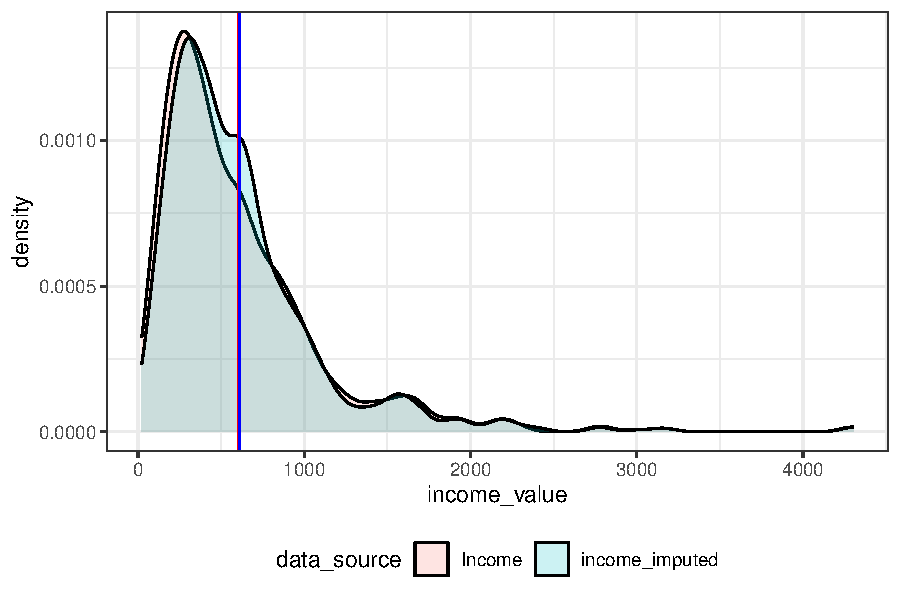
\includegraphics[width=0.7\linewidth,height=\textheight,keepaspectratio]{chapters/../figures/fig-ap3-mean-conditional-1.pdf}

}

\caption{\label{fig-ap3-mean-conditional}Distribución del ingreso
original e imputado por la media condicional}

\end{figure}%

El siguiente código computacional compara el ingreso original
(\texttt{Income}) y el completado con medias por estrato
(\texttt{income\_imputed}), desagregados por zona y sexo
(figura~\ref{fig-ap3-mean-conditional-groups}). Las medianas son
próximas y persisten algunas diferencias en la amplitud de las cajas. La
línea roja indica la media del ingreso original en toda la muestra.

\begin{Shaded}
\begin{Highlighting}[]
\NormalTok{conditional\_mean\_boxplot }\OtherTok{\textless{}{-}} \FunctionTok{ggplot}\NormalTok{(}
\NormalTok{  conditional\_mean\_plot\_data,}
  \FunctionTok{aes}\NormalTok{(}\AttributeTok{x =}\NormalTok{ data\_source, }\AttributeTok{y =}\NormalTok{ income\_value)}
\NormalTok{) }\SpecialCharTok{+}
  \FunctionTok{geom\_hline}\NormalTok{(}\AttributeTok{yintercept =} \FunctionTok{mean}\NormalTok{(survey\_data}\SpecialCharTok{$}\NormalTok{Income), }\AttributeTok{color =} \StringTok{"red"}\NormalTok{) }\SpecialCharTok{+}
  \FunctionTok{geom\_boxplot}\NormalTok{() }\SpecialCharTok{+}
  \FunctionTok{facet\_grid}\NormalTok{(Zone }\SpecialCharTok{\textasciitilde{}}\NormalTok{ Sex) }\SpecialCharTok{+}
  \FunctionTok{theme\_bw}\NormalTok{()}

\NormalTok{conditional\_mean\_boxplot}
\end{Highlighting}
\end{Shaded}

\begin{figure}[H]

\centering{

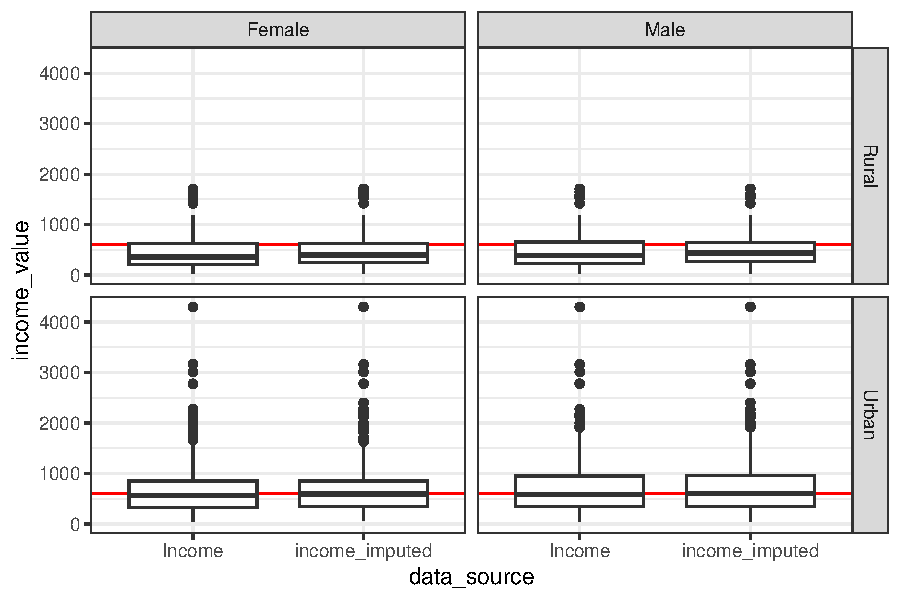
\includegraphics[width=0.7\linewidth,height=\textheight,keepaspectratio]{chapters/../figures/fig-ap3-mean-conditional-groups-1.pdf}

}

\caption{\label{fig-ap3-mean-conditional-groups}Ingreso original e
imputado por la media condicional, por zona y sexo}

\end{figure}%

\subsection{\texorpdfstring{Imputación por
\emph{hot-deck}}{Imputación por hot-deck}}\label{imputaciuxf3n-por-hot-deck}

La imputación por \emph{hot-deck} reemplaza los valores faltantes de una
unidad que no respondió (el receptor) con valores observados de otra
unidad (el donante). En la variante aleatoria no condicionada, el
donante se selecciona al azar entre todos los registros con información
disponible. Otras variantes restringen la selección a grupos con
características similares, como edad, sexo o zona de residencia, para
aprovechar su relación con la variable que se desea imputar.

El término \emph{hot-deck} hace referencia a las tarjetas perforadas
utilizadas en los primeros sistemas informáticos para almacenar y
recuperar datos. Esta técnica es relativamente simple y eficaz en
conjuntos de datos pequeños o medianos, y se utiliza con frecuencia en
encuestas y estudios de investigación social. Sin embargo, puede
resultar menos eficaz en conjuntos grandes o complejos cuando es difícil
encontrar observaciones similares o definir y medir las características
relevantes de manera confiable.

El siguiente código ilustra el hot-deck aleatorio no condicionado: para
cada ingreso faltante se selecciona un donante entre todos los registros
con ingreso observado, sin formar grupos ni comparar características
auxiliares.

\begin{Shaded}
\begin{Highlighting}[]
\NormalTok{donor\_indices }\OtherTok{\textless{}{-}} \FunctionTok{which}\NormalTok{(}\SpecialCharTok{!}\FunctionTok{is.na}\NormalTok{(survey\_data}\SpecialCharTok{$}\NormalTok{income\_missing))}
\NormalTok{recipient\_indices }\OtherTok{\textless{}{-}} \FunctionTok{which}\NormalTok{(}\FunctionTok{is.na}\NormalTok{(survey\_data}\SpecialCharTok{$}\NormalTok{income\_missing))}
\NormalTok{survey\_data}\SpecialCharTok{$}\NormalTok{income\_imputed }\OtherTok{\textless{}{-}}\NormalTok{ survey\_data}\SpecialCharTok{$}\NormalTok{income\_missing}

\FunctionTok{set.seed}\NormalTok{(}\DecValTok{1234}\NormalTok{)}
\ControlFlowTok{for}\NormalTok{ (i }\ControlFlowTok{in}\NormalTok{ recipient\_indices) \{}
\NormalTok{  donor\_index }\OtherTok{\textless{}{-}} \FunctionTok{sample}\NormalTok{(}\AttributeTok{x =}\NormalTok{ donor\_indices, }\AttributeTok{size =} \DecValTok{1}\NormalTok{)}
\NormalTok{  survey\_data}\SpecialCharTok{$}\NormalTok{income\_imputed[i] }\OtherTok{\textless{}{-}}\NormalTok{ survey\_data}\SpecialCharTok{$}\NormalTok{income\_missing[donor\_index]}
\NormalTok{\}}

\FunctionTok{sum}\NormalTok{(}\FunctionTok{is.na}\NormalTok{(survey\_data}\SpecialCharTok{$}\NormalTok{income\_imputed))}
\end{Highlighting}
\end{Shaded}

\begin{verbatim}
[1] 0
\end{verbatim}

El código anterior identifica las observaciones con y sin valores
faltantes en \texttt{income\_missing} y crea \texttt{income\_imputed}
para almacenar los resultados. Luego, un bucle \texttt{for} recorre las
observaciones receptoras. En cada iteración, la función \texttt{sample}
selecciona aleatoriamente un donante entre las observaciones con ingreso
disponible.

Una vez realizada la imputación, el siguiente código computacional
compara la media y la desviación estándar del ingreso original con las
del ingreso completado.

\begin{Shaded}
\begin{Highlighting}[]
\NormalTok{survey\_data }\SpecialCharTok{\%\textgreater{}\%}
  \FunctionTok{summarise}\NormalTok{(}
    \AttributeTok{income\_mean =} \FunctionTok{mean}\NormalTok{(Income),}
    \AttributeTok{income\_sd =} \FunctionTok{sd}\NormalTok{(Income),}
    \AttributeTok{imputed\_income\_mean =} \FunctionTok{mean}\NormalTok{(income\_imputed),}
    \AttributeTok{imputed\_income\_sd =} \FunctionTok{sd}\NormalTok{(income\_imputed)}
\NormalTok{  )}
\end{Highlighting}
\end{Shaded}

\begin{verbatim}
  income_mean income_sd imputed_income_mean imputed_income_sd
1         604       513                 618               528
\end{verbatim}

El sesgo relativo de la media del ingreso es del 2,32 \%. Al desagregar
los resultados por zona, se obtiene lo siguiente:

\begin{Shaded}
\begin{Highlighting}[]
\NormalTok{survey\_data }\SpecialCharTok{\%\textgreater{}\%}
  \FunctionTok{group\_by}\NormalTok{(Zone) }\SpecialCharTok{\%\textgreater{}\%}
  \FunctionTok{summarise}\NormalTok{(}
    \AttributeTok{income\_mean =} \FunctionTok{mean}\NormalTok{(Income),}
    \AttributeTok{income\_sd =} \FunctionTok{sd}\NormalTok{(Income),}
    \AttributeTok{imputed\_income\_mean =} \FunctionTok{mean}\NormalTok{(income\_imputed),}
    \AttributeTok{imputed\_income\_sd =} \FunctionTok{sd}\NormalTok{(income\_imputed)}
\NormalTok{  )}
\end{Highlighting}
\end{Shaded}

\begin{verbatim}
# A tibble: 2 x 5
  Zone  income_mean income_sd imputed_income_mean imputed_income_sd
  <chr>       <dbl>     <dbl>               <dbl>             <dbl>
1 Rural        469.      337.                504.              369.
2 Urban        731.      609.                726.              624.
\end{verbatim}

El sesgo relativo de la media del ingreso es del 7,37 \% en la zona
rural y del -0,71 \% en la urbana. El siguiente código computacional
extiende la comparación de estos resúmenes a los grupos definidos por
sexo.

\begin{Shaded}
\begin{Highlighting}[]
\NormalTok{survey\_data }\SpecialCharTok{\%\textgreater{}\%}
  \FunctionTok{group\_by}\NormalTok{(Sex) }\SpecialCharTok{\%\textgreater{}\%}
  \FunctionTok{summarise}\NormalTok{(}
    \AttributeTok{income\_mean =} \FunctionTok{mean}\NormalTok{(Income),}
    \AttributeTok{income\_sd =} \FunctionTok{sd}\NormalTok{(Income),}
    \AttributeTok{imputed\_income\_mean =} \FunctionTok{mean}\NormalTok{(income\_imputed),}
    \AttributeTok{imputed\_income\_sd =} \FunctionTok{sd}\NormalTok{(income\_imputed)}
\NormalTok{  )}
\end{Highlighting}
\end{Shaded}

\begin{verbatim}
# A tibble: 2 x 5
  Sex    income_mean income_sd imputed_income_mean imputed_income_sd
  <chr>        <dbl>     <dbl>               <dbl>             <dbl>
1 Female        589.      504.                603.              503.
2 Male          622.      523.                636.              556.
\end{verbatim}

El siguiente código computacional compara la densidad del ingreso
original (\texttt{Income}) con la del ingreso completado mediante
donantes aleatorios (\texttt{income\_imputed})
(figura~\ref{fig-ap3-hot-deck}). Las curvas prácticamente se superponen
en esta simulación, conservando la asimetría y la cola de ingresos
altos. Las líneas roja y azul representan las medias original e
imputada, respectivamente.

\begin{Shaded}
\begin{Highlighting}[]
\NormalTok{hot\_deck\_plot\_data }\OtherTok{\textless{}{-}}\NormalTok{ survey\_data }\SpecialCharTok{\%\textgreater{}\%}
\NormalTok{  dplyr}\SpecialCharTok{::}\FunctionTok{select}\NormalTok{(Zone, Sex, Income, income\_imputed) }\SpecialCharTok{\%\textgreater{}\%}
\NormalTok{  tidyr}\SpecialCharTok{::}\FunctionTok{gather}\NormalTok{(data\_source, income\_value, }\SpecialCharTok{{-}}\NormalTok{Zone, }\SpecialCharTok{{-}}\NormalTok{Sex)}

\NormalTok{hot\_deck\_density\_plot }\OtherTok{\textless{}{-}} \FunctionTok{ggplot}\NormalTok{(}
\NormalTok{  hot\_deck\_plot\_data,}
  \FunctionTok{aes}\NormalTok{(}\AttributeTok{x =}\NormalTok{ income\_value, }\AttributeTok{fill =}\NormalTok{ data\_source)}
\NormalTok{) }\SpecialCharTok{+}
  \FunctionTok{geom\_density}\NormalTok{(}\AttributeTok{alpha =} \FloatTok{0.2}\NormalTok{) }\SpecialCharTok{+}
  \FunctionTok{theme\_bw}\NormalTok{() }\SpecialCharTok{+}
  \FunctionTok{theme}\NormalTok{(}\AttributeTok{legend.position =} \StringTok{"bottom"}\NormalTok{) }\SpecialCharTok{+}
  \FunctionTok{geom\_vline}\NormalTok{(}\AttributeTok{xintercept =} \FunctionTok{mean}\NormalTok{(survey\_data}\SpecialCharTok{$}\NormalTok{Income), }\AttributeTok{color =} \StringTok{"red"}\NormalTok{) }\SpecialCharTok{+}
  \FunctionTok{geom\_vline}\NormalTok{(}
    \AttributeTok{xintercept =} \FunctionTok{mean}\NormalTok{(survey\_data}\SpecialCharTok{$}\NormalTok{income\_imputed),}
    \AttributeTok{color =} \StringTok{"blue"}
\NormalTok{  )}

\NormalTok{hot\_deck\_density\_plot}
\end{Highlighting}
\end{Shaded}

\begin{figure}[H]

\centering{

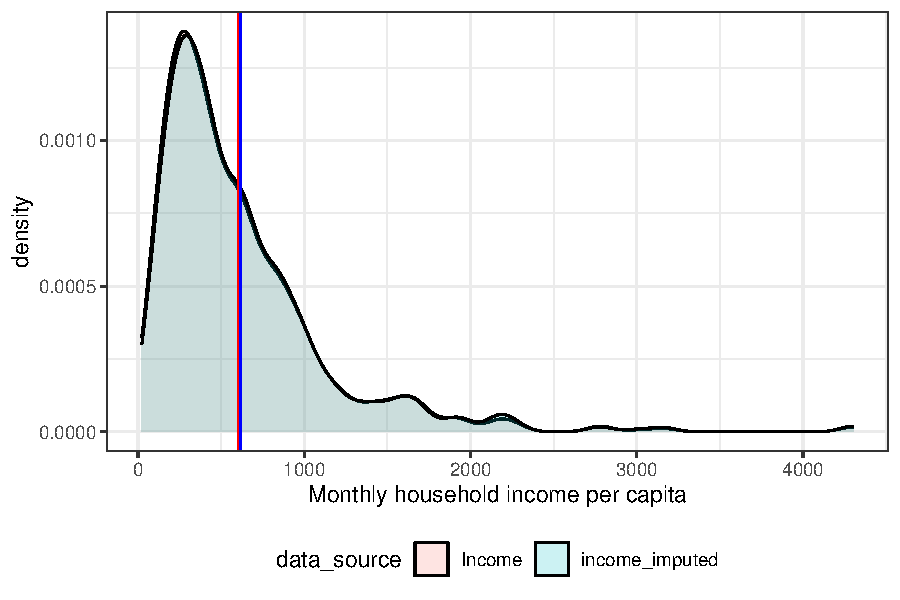
\includegraphics[width=0.7\linewidth,height=\textheight,keepaspectratio]{chapters/../figures/fig-ap3-hot-deck-1.pdf}

}

\caption{\label{fig-ap3-hot-deck}Distribución del ingreso original e
imputado mediante hot-deck}

\end{figure}%

\subsection{Imputación por
regresión}\label{imputaciuxf3n-por-regresiuxf3n}

La imputación por regresión utiliza las variables auxiliares disponibles
para predecir los valores faltantes de la variable de interés. Primero,
se identifican las variables predictoras relacionadas con ella. Luego,
se ajusta un modelo con los valores observados y se utilizan sus
coeficientes para predecir los valores faltantes.

El siguiente código computacional ajusta un modelo de regresión lineal
múltiple para imputar el ingreso, utilizando la zona, el sexo y el gasto
como covariables.

\begin{Shaded}
\begin{Highlighting}[]
\NormalTok{survey\_data}\SpecialCharTok{$}\NormalTok{income\_imputed }\OtherTok{\textless{}{-}}\NormalTok{ survey\_data}\SpecialCharTok{$}\NormalTok{income\_missing}
\NormalTok{observed\_data }\OtherTok{\textless{}{-}} \FunctionTok{filter}\NormalTok{(survey\_data, }\SpecialCharTok{!}\FunctionTok{is.na}\NormalTok{(income\_missing))}
\NormalTok{missing\_data }\OtherTok{\textless{}{-}} \FunctionTok{filter}\NormalTok{(survey\_data, }\FunctionTok{is.na}\NormalTok{(income\_missing))}

\NormalTok{imputation\_model }\OtherTok{\textless{}{-}} \FunctionTok{lm}\NormalTok{(}
\NormalTok{  Income }\SpecialCharTok{\textasciitilde{}}\NormalTok{ Zone }\SpecialCharTok{+}\NormalTok{ Sex }\SpecialCharTok{+}\NormalTok{ Expenditure,}
  \AttributeTok{data =}\NormalTok{ observed\_data}
\NormalTok{)}
\end{Highlighting}
\end{Shaded}

Una vez ajustado el modelo, el siguiente código computacional obtiene
las predicciones y las utiliza para completar los ingresos faltantes.

\begin{Shaded}
\begin{Highlighting}[]
\NormalTok{predicted\_income }\OtherTok{\textless{}{-}} \FunctionTok{predict}\NormalTok{(}
\NormalTok{  imputation\_model,}
  \AttributeTok{newdata =}\NormalTok{ missing\_data}
\NormalTok{)}
\NormalTok{missing\_data}\SpecialCharTok{$}\NormalTok{income\_imputed }\OtherTok{\textless{}{-}}\NormalTok{ predicted\_income}
\NormalTok{survey\_data }\OtherTok{\textless{}{-}} \FunctionTok{bind\_rows}\NormalTok{(observed\_data, missing\_data)}
\end{Highlighting}
\end{Shaded}

A continuación, se calculan la media y la desviación estándar de los
ingresos originales y de los completados por imputación:

\begin{Shaded}
\begin{Highlighting}[]
\NormalTok{survey\_data }\SpecialCharTok{\%\textgreater{}\%}
  \FunctionTok{summarise}\NormalTok{(}
    \AttributeTok{income\_mean =} \FunctionTok{mean}\NormalTok{(Income),}
    \AttributeTok{income\_sd =} \FunctionTok{sd}\NormalTok{(Income),}
    \AttributeTok{imputed\_income\_mean =} \FunctionTok{mean}\NormalTok{(income\_imputed),}
    \AttributeTok{imputed\_income\_sd =} \FunctionTok{sd}\NormalTok{(income\_imputed)}
\NormalTok{  )}
\end{Highlighting}
\end{Shaded}

\begin{verbatim}
  income_mean income_sd imputed_income_mean imputed_income_sd
1         604       513                 612               498
\end{verbatim}

El sesgo relativo de la media del ingreso es del 1,24 \%. El siguiente
código computacional compara por zona los resúmenes del ingreso original
y del completado por regresión.

\begin{Shaded}
\begin{Highlighting}[]
\NormalTok{survey\_data }\SpecialCharTok{\%\textgreater{}\%}
  \FunctionTok{group\_by}\NormalTok{(Zone) }\SpecialCharTok{\%\textgreater{}\%}
  \FunctionTok{summarise}\NormalTok{(}
    \AttributeTok{income\_mean =} \FunctionTok{mean}\NormalTok{(Income),}
    \AttributeTok{income\_sd =} \FunctionTok{sd}\NormalTok{(Income),}
    \AttributeTok{imputed\_income\_mean =} \FunctionTok{mean}\NormalTok{(income\_imputed),}
    \AttributeTok{imputed\_income\_sd =} \FunctionTok{sd}\NormalTok{(income\_imputed)}
\NormalTok{  )}
\end{Highlighting}
\end{Shaded}

\begin{verbatim}
# A tibble: 2 x 5
  Zone  income_mean income_sd imputed_income_mean imputed_income_sd
  <chr>       <dbl>     <dbl>               <dbl>             <dbl>
1 Rural        469.      337.                476.              317.
2 Urban        731.      609.                739.              595.
\end{verbatim}

El siguiente código computacional compara las densidades del ingreso
original (\texttt{Income}) y del completado con predicciones del modelo
de regresión (\texttt{income\_imputed})
(figura~\ref{fig-ap3-regression}). La forma general es similar, aunque
aparecen diferencias alrededor del tramo central de la distribución. Las
líneas roja y azul indican las medias original e imputada,
respectivamente.

\begin{Shaded}
\begin{Highlighting}[]
\NormalTok{regression\_plot\_data }\OtherTok{\textless{}{-}}\NormalTok{ survey\_data }\SpecialCharTok{\%\textgreater{}\%}
\NormalTok{  dplyr}\SpecialCharTok{::}\FunctionTok{select}\NormalTok{(Zone, Sex, Income, income\_imputed) }\SpecialCharTok{\%\textgreater{}\%}
\NormalTok{  tidyr}\SpecialCharTok{::}\FunctionTok{gather}\NormalTok{(data\_source, income\_value, }\SpecialCharTok{{-}}\NormalTok{Zone, }\SpecialCharTok{{-}}\NormalTok{Sex)}

\NormalTok{regression\_density\_plot }\OtherTok{\textless{}{-}} \FunctionTok{ggplot}\NormalTok{(}
\NormalTok{  regression\_plot\_data,}
  \FunctionTok{aes}\NormalTok{(}\AttributeTok{x =}\NormalTok{ income\_value, }\AttributeTok{fill =}\NormalTok{ data\_source)}
\NormalTok{) }\SpecialCharTok{+}
  \FunctionTok{geom\_density}\NormalTok{(}\AttributeTok{alpha =} \FloatTok{0.2}\NormalTok{) }\SpecialCharTok{+}
  \FunctionTok{theme\_bw}\NormalTok{() }\SpecialCharTok{+}
  \FunctionTok{theme}\NormalTok{(}\AttributeTok{legend.position =} \StringTok{"bottom"}\NormalTok{) }\SpecialCharTok{+}
  \FunctionTok{geom\_vline}\NormalTok{(}\AttributeTok{xintercept =} \FunctionTok{mean}\NormalTok{(survey\_data}\SpecialCharTok{$}\NormalTok{Income), }\AttributeTok{color =} \StringTok{"red"}\NormalTok{) }\SpecialCharTok{+}
  \FunctionTok{geom\_vline}\NormalTok{(}
    \AttributeTok{xintercept =} \FunctionTok{mean}\NormalTok{(survey\_data}\SpecialCharTok{$}\NormalTok{income\_imputed),}
    \AttributeTok{color =} \StringTok{"blue"}
\NormalTok{  )}

\NormalTok{regression\_density\_plot}
\end{Highlighting}
\end{Shaded}

\begin{figure}[H]

\centering{

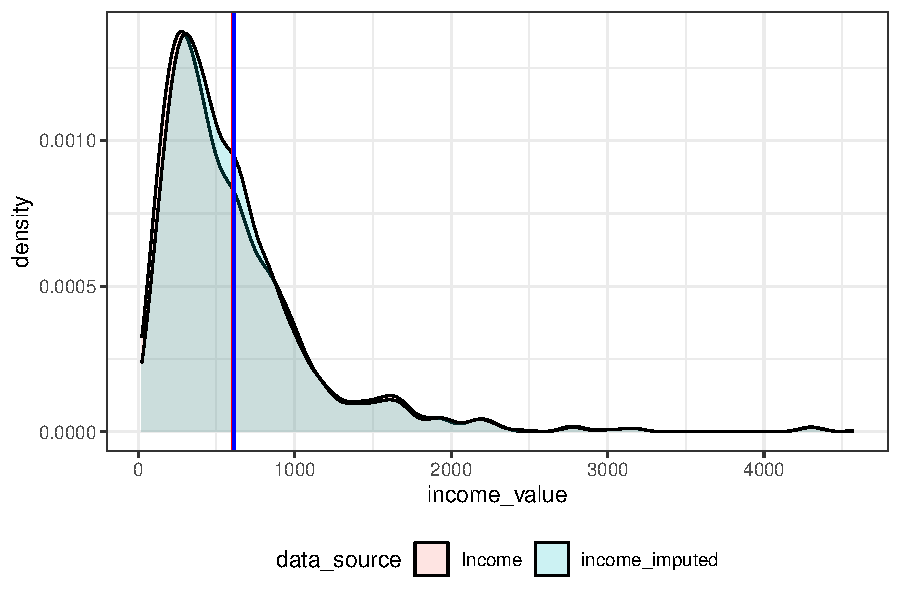
\includegraphics[width=0.7\linewidth,height=\textheight,keepaspectratio]{chapters/../figures/fig-ap3-regression-1.pdf}

}

\caption{\label{fig-ap3-regression}Distribución del ingreso original e
imputado por regresión}

\end{figure}%

\subsection{Imputación por el vecino más
cercano}\label{imputaciuxf3n-por-el-vecino-muxe1s-cercano}

La imputación por el vecino más cercano reemplaza los valores faltantes
con información de observaciones similares. El método se basa en la idea
de que los registros con características semejantes tienden a tener
valores similares en la variable de interés. En su versión con varios
vecinos, se identifican los \(k\) registros más próximos al receptor y
se utilizan sus valores para estimar el dato faltante.

Para calcular la similitud entre observaciones, se pueden utilizar
diferentes medidas de distancia, como la distancia euclidiana o la
distancia de Manhattan. La técnica también permite ajustar el valor de
\(k\), que representa el número de vecinos más cercanos utilizados para
estimar el valor faltante.

Este método es relativamente simple y fácil de implementar. Sin embargo,
su eficacia depende de la cantidad y la calidad de los datos
disponibles, así como del número de vecinos y de la medida de distancia
elegidos. Por ello, conviene evaluar tanto la calidad de los datos como
los resultados de la imputación.

La aplicación del método con un solo vecino comprende tres pasos:

\begin{enumerate}
\def\labelenumi{\arabic{enumi}.}
\tightlist
\item
  Definir una medida de distancia, como la euclidiana, para comparar las
  observaciones.
\item
  Identificar, para cada receptor, el donante más cercano según la
  medida elegida.
\item
  Reemplazar el valor faltante con el valor observado del donante.
\end{enumerate}

En el siguiente ejemplo, se imputa el ingreso utilizando el gasto del
individuo como variable auxiliar y la distancia euclidiana como medida
de similitud.

\begin{Shaded}
\begin{Highlighting}[]
\NormalTok{survey\_data}\SpecialCharTok{$}\NormalTok{income\_imputed }\OtherTok{\textless{}{-}}\NormalTok{ survey\_data}\SpecialCharTok{$}\NormalTok{income\_missing}
\NormalTok{observed\_data }\OtherTok{\textless{}{-}} \FunctionTok{filter}\NormalTok{(survey\_data, }\SpecialCharTok{!}\FunctionTok{is.na}\NormalTok{(income\_missing))}
\NormalTok{missing\_data }\OtherTok{\textless{}{-}} \FunctionTok{filter}\NormalTok{(survey\_data, }\FunctionTok{is.na}\NormalTok{(income\_missing))}

\ControlFlowTok{for}\NormalTok{ (i }\ControlFlowTok{in} \FunctionTok{seq\_len}\NormalTok{(}\FunctionTok{nrow}\NormalTok{(missing\_data))) \{}
\NormalTok{  recipient\_expenditure }\OtherTok{\textless{}{-}}\NormalTok{ missing\_data}\SpecialCharTok{$}\NormalTok{Expenditure[[i]]}
\NormalTok{  donor\_index }\OtherTok{\textless{}{-}} \FunctionTok{which.min}\NormalTok{(}\FunctionTok{abs}\NormalTok{(recipient\_expenditure }\SpecialCharTok{{-}}\NormalTok{ observed\_data}\SpecialCharTok{$}\NormalTok{Expenditure))}
\NormalTok{  missing\_data}\SpecialCharTok{$}\NormalTok{income\_imputed[[i]] }\OtherTok{\textless{}{-}}
\NormalTok{    observed\_data}\SpecialCharTok{$}\NormalTok{income\_missing[[donor\_index]]}
\NormalTok{\}}

\NormalTok{survey\_data }\OtherTok{\textless{}{-}} \FunctionTok{bind\_rows}\NormalTok{(observed\_data, missing\_data)}
\end{Highlighting}
\end{Shaded}

Las medias y las desviaciones estándar de los ingresos originales y de
los completados por imputación se calculan de la siguiente manera:

\begin{Shaded}
\begin{Highlighting}[]
\NormalTok{survey\_data }\SpecialCharTok{\%\textgreater{}\%}
  \FunctionTok{summarise}\NormalTok{(}
    \AttributeTok{income\_mean =} \FunctionTok{mean}\NormalTok{(Income),}
    \AttributeTok{income\_sd =} \FunctionTok{sd}\NormalTok{(Income),}
    \AttributeTok{imputed\_income\_mean =} \FunctionTok{mean}\NormalTok{(income\_imputed),}
    \AttributeTok{imputed\_income\_sd =} \FunctionTok{sd}\NormalTok{(income\_imputed)}
\NormalTok{  )}
\end{Highlighting}
\end{Shaded}

\begin{verbatim}
  income_mean income_sd imputed_income_mean imputed_income_sd
1         604       513                 611               514
\end{verbatim}

La media imputada supera a la original en aproximadamente 6,3 unidades
monetarias. El siguiente código computacional compara por zona los
resúmenes del ingreso original y del completado con donantes.

\begin{Shaded}
\begin{Highlighting}[]
\NormalTok{survey\_data }\SpecialCharTok{\%\textgreater{}\%}
  \FunctionTok{group\_by}\NormalTok{(Zone) }\SpecialCharTok{\%\textgreater{}\%}
  \FunctionTok{summarise}\NormalTok{(}
    \AttributeTok{income\_mean =} \FunctionTok{mean}\NormalTok{(Income),}
    \AttributeTok{income\_sd =} \FunctionTok{sd}\NormalTok{(Income),}
    \AttributeTok{imputed\_income\_mean =} \FunctionTok{mean}\NormalTok{(income\_imputed),}
    \AttributeTok{imputed\_income\_sd =} \FunctionTok{sd}\NormalTok{(income\_imputed)}
\NormalTok{  )}
\end{Highlighting}
\end{Shaded}

\begin{verbatim}
# A tibble: 2 x 5
  Zone  income_mean income_sd imputed_income_mean imputed_income_sd
  <chr>       <dbl>     <dbl>               <dbl>             <dbl>
1 Rural        469.      337.                478.              344.
2 Urban        731.      609.                735.              607.
\end{verbatim}

La media imputada supera a la original en aproximadamente 8,8 unidades
monetarias en la zona rural y 3,9 en la urbana.

El siguiente código computacional compara la densidad del ingreso
original (\texttt{Income}) y la del ingreso imputado con donantes de
gasto similar (\texttt{income\_imputed})
(figura~\ref{fig-ap3-nearest-neighbor}). Las curvas son muy próximas y
conservan la cola de ingresos altos. Las líneas roja y azul muestran las
medias original e imputada, respectivamente.

\begin{Shaded}
\begin{Highlighting}[]
\NormalTok{nearest\_neighbor\_plot\_data }\OtherTok{\textless{}{-}}\NormalTok{ survey\_data }\SpecialCharTok{\%\textgreater{}\%}
\NormalTok{  dplyr}\SpecialCharTok{::}\FunctionTok{select}\NormalTok{(Zone, Sex, Income, income\_imputed) }\SpecialCharTok{\%\textgreater{}\%}
\NormalTok{  tidyr}\SpecialCharTok{::}\FunctionTok{gather}\NormalTok{(data\_source, income\_value, }\SpecialCharTok{{-}}\NormalTok{Zone, }\SpecialCharTok{{-}}\NormalTok{Sex)}

\NormalTok{nearest\_neighbor\_density\_plot }\OtherTok{\textless{}{-}} \FunctionTok{ggplot}\NormalTok{(}
\NormalTok{  nearest\_neighbor\_plot\_data,}
  \FunctionTok{aes}\NormalTok{(}\AttributeTok{x =}\NormalTok{ income\_value, }\AttributeTok{fill =}\NormalTok{ data\_source)}
\NormalTok{) }\SpecialCharTok{+}
  \FunctionTok{geom\_density}\NormalTok{(}\AttributeTok{alpha =} \FloatTok{0.2}\NormalTok{) }\SpecialCharTok{+}
  \FunctionTok{theme\_bw}\NormalTok{() }\SpecialCharTok{+}
  \FunctionTok{theme}\NormalTok{(}\AttributeTok{legend.position =} \StringTok{"bottom"}\NormalTok{) }\SpecialCharTok{+}
  \FunctionTok{geom\_vline}\NormalTok{(}\AttributeTok{xintercept =} \FunctionTok{mean}\NormalTok{(survey\_data}\SpecialCharTok{$}\NormalTok{Income), }\AttributeTok{color =} \StringTok{"red"}\NormalTok{) }\SpecialCharTok{+}
  \FunctionTok{geom\_vline}\NormalTok{(}
    \AttributeTok{xintercept =} \FunctionTok{mean}\NormalTok{(survey\_data}\SpecialCharTok{$}\NormalTok{income\_imputed),}
    \AttributeTok{color =} \StringTok{"blue"}
\NormalTok{  )}

\NormalTok{nearest\_neighbor\_density\_plot}
\end{Highlighting}
\end{Shaded}

\begin{figure}[H]

\centering{

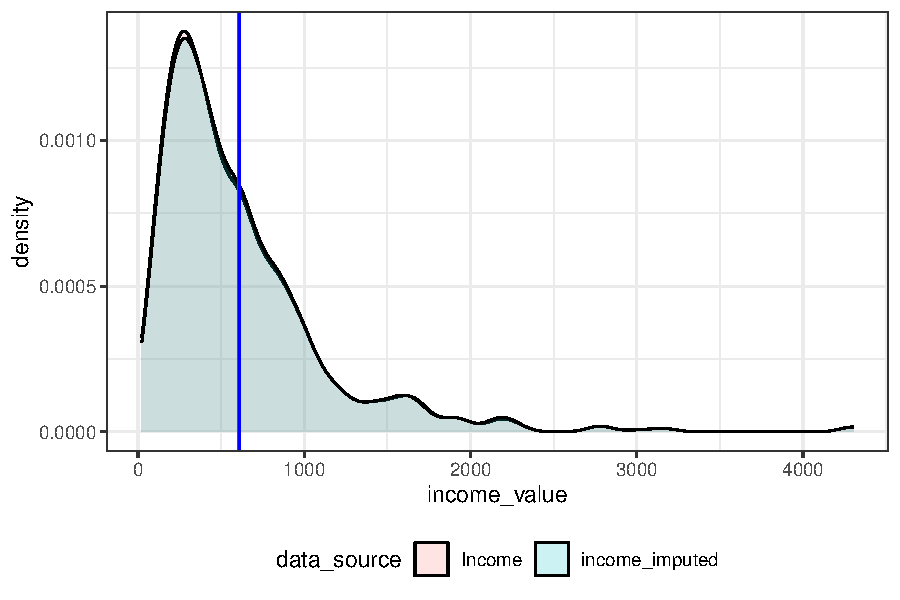
\includegraphics[width=0.7\linewidth,height=\textheight,keepaspectratio]{chapters/../figures/fig-ap3-nearest-neighbor-1.pdf}

}

\caption{\label{fig-ap3-nearest-neighbor}Distribución del ingreso
original e imputado por el vecino más cercano}

\end{figure}%

\subsection{Imputación por el vecino más cercano con
regresión}\label{imputaciuxf3n-por-el-vecino-muxe1s-cercano-con-regresiuxf3n}

La imputación por el vecino más cercano con regresión comprende los
siguientes pasos:

\begin{enumerate}
\def\labelenumi{\arabic{enumi}.}
\tightlist
\item
  Ajustar un modelo de regresión entre la variable de interés y las
  covariables auxiliares.
\item
  Predecir los valores de la variable de interés para las observaciones
  con y sin datos faltantes.
\item
  Comparar las predicciones de los posibles donantes con las de los
  receptores.
\item
  Identificar, para cada receptor, el donante cuya predicción sea más
  cercana a la suya.
\item
  Reemplazar el valor faltante con la información observada proveniente
  del donante.
\end{enumerate}

En el siguiente ejemplo, se imputan los ingresos mediante un modelo que
utiliza el sexo, la zona y el gasto como covariables:

\begin{Shaded}
\begin{Highlighting}[]
\NormalTok{survey\_data}\SpecialCharTok{$}\NormalTok{income\_imputed }\OtherTok{\textless{}{-}}\NormalTok{ survey\_data}\SpecialCharTok{$}\NormalTok{income\_missing}
\NormalTok{observed\_data }\OtherTok{\textless{}{-}} \FunctionTok{filter}\NormalTok{(survey\_data, }\SpecialCharTok{!}\FunctionTok{is.na}\NormalTok{(income\_missing))}
\NormalTok{missing\_data }\OtherTok{\textless{}{-}} \FunctionTok{filter}\NormalTok{(survey\_data, }\FunctionTok{is.na}\NormalTok{(income\_missing))}

\NormalTok{imputation\_model }\OtherTok{\textless{}{-}} \FunctionTok{lm}\NormalTok{(}
\NormalTok{  Income }\SpecialCharTok{\textasciitilde{}}\NormalTok{ Zone }\SpecialCharTok{+}\NormalTok{ Sex }\SpecialCharTok{+}\NormalTok{ Expenditure,}
  \AttributeTok{data =}\NormalTok{ observed\_data}
\NormalTok{)}
\end{Highlighting}
\end{Shaded}

Con el modelo ajustado, el siguiente código computacional predice los
ingresos de las observaciones con y sin datos faltantes. Para cada
receptor, identifica al donante con la predicción más cercana y utiliza
su ingreso observado para completar el valor faltante.

\begin{Shaded}
\begin{Highlighting}[]
\NormalTok{observed\_predictions }\OtherTok{\textless{}{-}} \FunctionTok{predict}\NormalTok{(}
\NormalTok{  imputation\_model,}
  \AttributeTok{newdata =}\NormalTok{ observed\_data}
\NormalTok{)}
\NormalTok{missing\_predictions }\OtherTok{\textless{}{-}} \FunctionTok{predict}\NormalTok{(}
\NormalTok{  imputation\_model,}
  \AttributeTok{newdata =}\NormalTok{ missing\_data}
\NormalTok{)}

\ControlFlowTok{for}\NormalTok{ (i }\ControlFlowTok{in} \FunctionTok{seq\_len}\NormalTok{(}\FunctionTok{nrow}\NormalTok{(missing\_data))) \{}
\NormalTok{  donor\_index }\OtherTok{\textless{}{-}} \FunctionTok{which.min}\NormalTok{(}\FunctionTok{abs}\NormalTok{(missing\_predictions[i] }\SpecialCharTok{{-}}\NormalTok{ observed\_predictions))}
\NormalTok{  missing\_data}\SpecialCharTok{$}\NormalTok{income\_imputed[[i]] }\OtherTok{\textless{}{-}}
\NormalTok{    observed\_data}\SpecialCharTok{$}\NormalTok{income\_missing[[donor\_index]]}
\NormalTok{\}}

\NormalTok{survey\_data }\OtherTok{\textless{}{-}} \FunctionTok{bind\_rows}\NormalTok{(observed\_data, missing\_data)}
\end{Highlighting}
\end{Shaded}

Como en los ejemplos anteriores, el siguiente código computacional
compara la media y la desviación estándar del ingreso original con las
del ingreso completado, en este caso mediante donantes seleccionados por
la proximidad de sus predicciones.

\begin{Shaded}
\begin{Highlighting}[]
\NormalTok{survey\_data }\SpecialCharTok{\%\textgreater{}\%}
  \FunctionTok{summarise}\NormalTok{(}
    \AttributeTok{income\_mean =} \FunctionTok{mean}\NormalTok{(Income),}
    \AttributeTok{income\_sd =} \FunctionTok{sd}\NormalTok{(Income),}
    \AttributeTok{imputed\_income\_mean =} \FunctionTok{mean}\NormalTok{(income\_imputed),}
    \AttributeTok{imputed\_income\_sd =} \FunctionTok{sd}\NormalTok{(income\_imputed)}
\NormalTok{  )}
\end{Highlighting}
\end{Shaded}

\begin{verbatim}
  income_mean income_sd imputed_income_mean imputed_income_sd
1         604       513                 608               516
\end{verbatim}

La diferencia entre la media del ingreso original y la obtenida tras la
imputación es de aproximadamente 4,0 unidades monetarias.

El siguiente código computacional compara el ingreso original
(\texttt{Income}) con el completado mediante donantes cuyas predicciones
son próximas a las del receptor (\texttt{income\_imputed})
(figura~\ref{fig-ap3-nearest-neighbor-regression}). Las densidades
prácticamente se superponen en esta simulación. Las líneas roja y azul
representan las medias original e imputada, respectivamente.

\begin{Shaded}
\begin{Highlighting}[]
\NormalTok{predictive\_matching\_plot\_data }\OtherTok{\textless{}{-}}\NormalTok{ survey\_data }\SpecialCharTok{\%\textgreater{}\%}
\NormalTok{  dplyr}\SpecialCharTok{::}\FunctionTok{select}\NormalTok{(Zone, Sex, Income, income\_imputed) }\SpecialCharTok{\%\textgreater{}\%}
\NormalTok{  tidyr}\SpecialCharTok{::}\FunctionTok{gather}\NormalTok{(data\_source, income\_value, }\SpecialCharTok{{-}}\NormalTok{Zone, }\SpecialCharTok{{-}}\NormalTok{Sex)}

\NormalTok{predictive\_matching\_density\_plot }\OtherTok{\textless{}{-}} \FunctionTok{ggplot}\NormalTok{(}
\NormalTok{  predictive\_matching\_plot\_data,}
  \FunctionTok{aes}\NormalTok{(}\AttributeTok{x =}\NormalTok{ income\_value, }\AttributeTok{fill =}\NormalTok{ data\_source)}
\NormalTok{) }\SpecialCharTok{+}
  \FunctionTok{geom\_density}\NormalTok{(}\AttributeTok{alpha =} \FloatTok{0.2}\NormalTok{) }\SpecialCharTok{+}
  \FunctionTok{theme\_bw}\NormalTok{() }\SpecialCharTok{+}
  \FunctionTok{theme}\NormalTok{(}\AttributeTok{legend.position =} \StringTok{"bottom"}\NormalTok{) }\SpecialCharTok{+}
  \FunctionTok{geom\_vline}\NormalTok{(}\AttributeTok{xintercept =} \FunctionTok{mean}\NormalTok{(survey\_data}\SpecialCharTok{$}\NormalTok{Income), }\AttributeTok{color =} \StringTok{"red"}\NormalTok{) }\SpecialCharTok{+}
  \FunctionTok{geom\_vline}\NormalTok{(}
    \AttributeTok{xintercept =} \FunctionTok{mean}\NormalTok{(survey\_data}\SpecialCharTok{$}\NormalTok{income\_imputed),}
    \AttributeTok{color =} \StringTok{"blue"}
\NormalTok{  )}

\NormalTok{predictive\_matching\_density\_plot}
\end{Highlighting}
\end{Shaded}

\begin{figure}[H]

\centering{

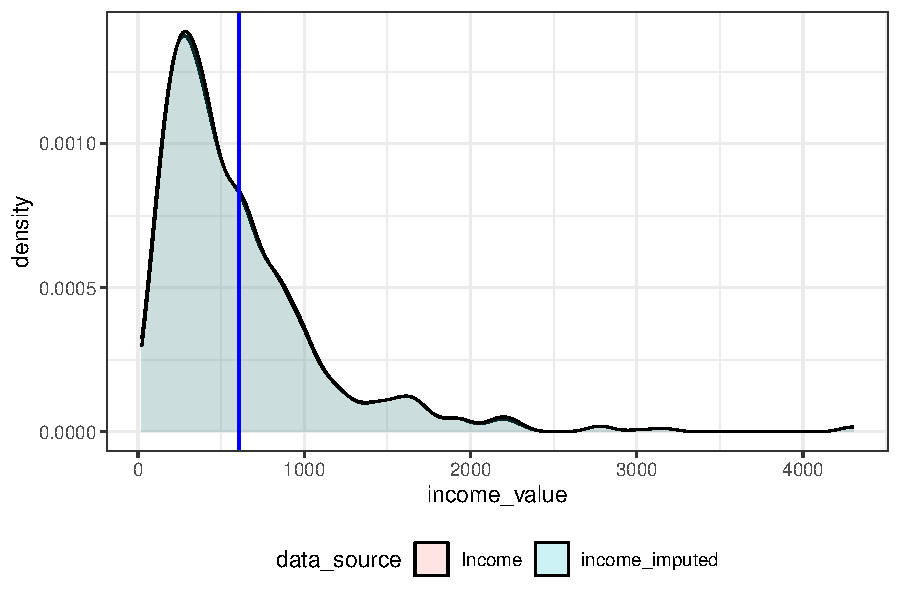
\includegraphics[width=0.7\linewidth,height=\textheight,keepaspectratio]{chapters/../figures/fig-ap3-nearest-neighbor-regression-1.pdf}

}

\caption{\label{fig-ap3-nearest-neighbor-regression}Distribución del
ingreso original e imputado por el vecino más cercano con regresión}

\end{figure}%

\subsection{Imputación múltiple}\label{imputaciuxf3n-muxfaltiple}

La imputación múltiple crea varias copias del conjunto de datos y
completa los valores faltantes de cada una mediante modelos estadísticos
basados en las relaciones entre las variables. Cada copia se analiza por
separado y los resultados se combinan para obtener una estimación final
que refleje la incertidumbre asociada con la imputación.

La imputación múltiple permite tratar los datos faltantes y puede
ofrecer resultados más precisos y menos sesgados que la eliminación de
las observaciones incompletas. Sin embargo, requiere recursos
computacionales y conocimientos estadísticos para su aplicación
adecuada. Esta técnica fue propuesta por Rubin
(\citeproc{ref-rubin1987multiple}{1987}) y consiste en generar \(M > 1\)
conjuntos de valores para los datos faltantes.

Para ilustrar el método, se considera un conjunto de \(n\) observaciones
de dos variables, \(X\) e \(Y\), relacionadas mediante el siguiente
modelo de regresión lineal simple:

\[y_i = \beta x_i + \varepsilon_i\]

El modelo se aplica a cada individuo \(i = 1, \ldots, n\), con errores
de distribución normal tales que \(E(\varepsilon) = 0\) y
\(Var(\varepsilon) = \sigma ^2\). Se define \(Y_{Obs}\) como un vector
que contiene los valores observados para un conjunto de individuos de
tamaño \(n_1\), y \(Y_{NoObs}\) como el vector de los valores no
observados de tamaño \(n_0\), es decir, \(n_1 + n_0 = n\). Además, se
supone que fue posible observar los valores de la covariable \(X\) para
todos los individuos en la muestra.

Los conjuntos completados se analizan por separado. Luego se combinan
las estimaciones del parámetro de interés y sus varianzas, conservando
la información sobre la variación entre imputaciones. Para la pendiente
de la regresión lineal simple \(\beta\), la esperanza condicional se
expresa como:

\[E(\hat{\beta} | Y_{obs}) = E(E(\hat{\beta} | Y_{obs}, Y_{mis}) | Y_{obs})\]

Esta expresión se estima mediante el promedio de las \(M\) estimaciones
puntuales de \(\hat{\beta}\) sobre las \(M\) imputaciones, dado por:

\begin{equation}\protect\phantomsection\label{eq-estimador-imputacion-multiple}{\bar{\hat{\beta}} = \frac{1}{M} \sum_{m = 1} ^ M \hat{\beta}_m}\end{equation}

La varianza estimada al utilizar la metodología de imputación múltiple
está dada por la siguiente expresión:

\[
V(\hat{\beta} | Y_{obs}) = E(V(\hat{\beta} | Y_{obs}, Y_{mis}) | Y_{obs}) +
V(E(\hat{\beta} | Y_{obs}, Y_{mis}) | Y_{obs})
\]

El primer término de la expresión anterior se estima como el promedio de
las varianzas muestrales de \(\hat{\beta}\) sobre las \(M\)
imputaciones, dado por:

\[\bar{U} = \frac{1}{M} \sum_{m = 1} ^ M \widehat{Var}(\hat{\beta}_m)\]

El segundo término se estima como la varianza muestral de las \(M\)
estimaciones puntuales de \(\hat{\beta}\) sobre las \(M\) imputaciones,
dada por:

\[B = \frac{1}{M-1} \sum_{m = 1} ^ M (\hat{\beta}_m - \bar{\hat{\beta}})^2\]

Es necesario tener en cuenta un factor de corrección (puesto que \(M\)
es finito). Por tanto, la estimación del segundo término viene dada por
la siguiente expresión:

\[
(1 + \frac{1}{M}) B
\]

Por tanto, la varianza estimada es igual a:
\begin{equation}\protect\phantomsection\label{eq-varianza-imputacion-multiple}{\hat{V}(\hat{\beta} | Y_{obs}) = \bar{U} + (1 + \frac{1}{M}) B}\end{equation}

El siguiente ejemplo aplica la imputación múltiple a los datos de la
encuesta:

\begin{Shaded}
\begin{Highlighting}[]
\NormalTok{survey\_data}\SpecialCharTok{$}\NormalTok{income\_imputed }\OtherTok{\textless{}{-}}\NormalTok{ survey\_data}\SpecialCharTok{$}\NormalTok{income\_missing}
\NormalTok{survey\_data}\SpecialCharTok{$}\NormalTok{employment\_imputed }\OtherTok{\textless{}{-}}\NormalTok{ survey\_data}\SpecialCharTok{$}\NormalTok{employment\_missing}
\NormalTok{observed\_data }\OtherTok{\textless{}{-}} \FunctionTok{filter}\NormalTok{(survey\_data, }\SpecialCharTok{!}\FunctionTok{is.na}\NormalTok{(income\_missing))}
\NormalTok{missing\_data }\OtherTok{\textless{}{-}} \FunctionTok{filter}\NormalTok{(survey\_data, }\FunctionTok{is.na}\NormalTok{(income\_missing))}
\NormalTok{n\_missing }\OtherTok{\textless{}{-}} \FunctionTok{nrow}\NormalTok{(missing\_data)}
\NormalTok{n\_observed }\OtherTok{\textless{}{-}} \FunctionTok{nrow}\NormalTok{(observed\_data)}
\end{Highlighting}
\end{Shaded}

Primero, se separan las observaciones con y sin valores faltantes y se
calcula el número de observaciones de cada grupo. El siguiente código
computacional genera los valores imputados a partir del modelo y los
incorpora a los conjuntos de datos completados.

\begin{Shaded}
\begin{Highlighting}[]
\NormalTok{n\_imputations }\OtherTok{\textless{}{-}} \DecValTok{10}
\FunctionTok{set.seed}\NormalTok{(}\DecValTok{1234}\NormalTok{)}

\ControlFlowTok{for}\NormalTok{ (i }\ControlFlowTok{in} \FunctionTok{seq\_len}\NormalTok{(n\_imputations)) \{}
\NormalTok{  imputation\_column }\OtherTok{\textless{}{-}} \FunctionTok{paste0}\NormalTok{(}\StringTok{"income\_draw\_"}\NormalTok{, i)}

\NormalTok{  bootstrap\_data }\OtherTok{\textless{}{-}}\NormalTok{ observed\_data }\SpecialCharTok{\%\textgreater{}\%}
    \FunctionTok{sample\_n}\NormalTok{(}\AttributeTok{size =}\NormalTok{ n\_observed, }\AttributeTok{replace =} \ConstantTok{TRUE}\NormalTok{)}

\NormalTok{  imputation\_model }\OtherTok{\textless{}{-}} \FunctionTok{lm}\NormalTok{(}
\NormalTok{    Income }\SpecialCharTok{\textasciitilde{}}\NormalTok{ Zone }\SpecialCharTok{+}\NormalTok{ Sex }\SpecialCharTok{+}\NormalTok{ Expenditure,}
    \AttributeTok{data =}\NormalTok{ bootstrap\_data}
\NormalTok{  )}

\NormalTok{  missing\_data[[imputation\_column]] }\OtherTok{\textless{}{-}} \FunctionTok{predict}\NormalTok{(}
\NormalTok{    imputation\_model,}
\NormalTok{    missing\_data}
\NormalTok{  )}
\NormalTok{  observed\_data[[imputation\_column]] }\OtherTok{\textless{}{-}}\NormalTok{ observed\_data}\SpecialCharTok{$}\NormalTok{Income}
\NormalTok{\}}
\end{Highlighting}
\end{Shaded}

El código anterior ajusta modelos de regresión lineal con
\texttt{Income} como variable de respuesta y \texttt{Zone}, \texttt{Sex}
y \texttt{Expenditure} como covariables. Estos modelos permiten predecir
los ingresos faltantes en \texttt{missing\_data}. El siguiente código
computacional permite revisar los ingresos originales junto con algunos
de los valores imputados.

\begin{Shaded}
\begin{Highlighting}[]
\NormalTok{dplyr}\SpecialCharTok{::}\FunctionTok{select}\NormalTok{(missing\_data, Income, }\FunctionTok{matches}\NormalTok{(}\StringTok{"income\_draw\_"}\NormalTok{))[}\DecValTok{1}\SpecialCharTok{:}\DecValTok{10}\NormalTok{, }\DecValTok{1}\SpecialCharTok{:}\DecValTok{4}\NormalTok{]}
\end{Highlighting}
\end{Shaded}

\begin{verbatim}
   Income income_draw_1 income_draw_2 income_draw_3
1   409.9           550           566           568
2   409.9           561           529           542
3    90.9           211           226           164
4    90.9           221           189           138
5    90.9           211           226           164
6   135.3           223           238           178
7   135.3           223           238           178
8  1539.8           785           801           847
9   336.0           508           473           440
10  685.5           593           558           541
\end{verbatim}

El siguiente código computacional compara la densidad del ingreso
original, representada por la línea negra, con las de los 10 conjuntos
completados, representadas por las líneas de colores
(\texttt{income\_draw\_1} a income\_draw\_10)
(figura~\ref{fig-ap3-imputation-multiple}). Las curvas mantienen una
forma similar, con pequeñas diferencias en el tramo central que reflejan
la variación entre las imputaciones.

\begin{Shaded}
\begin{Highlighting}[]
\NormalTok{survey\_data }\OtherTok{\textless{}{-}} \FunctionTok{bind\_rows}\NormalTok{(observed\_data, missing\_data)}

\NormalTok{multiple\_imputation\_plot\_data }\OtherTok{\textless{}{-}}\NormalTok{ survey\_data }\SpecialCharTok{\%\textgreater{}\%}
\NormalTok{  dplyr}\SpecialCharTok{::}\FunctionTok{select}\NormalTok{(Zone, Sex, }\FunctionTok{matches}\NormalTok{(}\StringTok{"income\_draw\_"}\NormalTok{)) }\SpecialCharTok{\%\textgreater{}\%}
\NormalTok{  tidyr}\SpecialCharTok{::}\FunctionTok{gather}\NormalTok{(data\_source, income\_value, }\SpecialCharTok{{-}}\NormalTok{Zone, }\SpecialCharTok{{-}}\NormalTok{Sex)}

\NormalTok{multiple\_imputation\_density\_plot }\OtherTok{\textless{}{-}} \FunctionTok{ggplot}\NormalTok{(}
\NormalTok{  multiple\_imputation\_plot\_data,}
  \FunctionTok{aes}\NormalTok{(}\AttributeTok{x =}\NormalTok{ income\_value, }\AttributeTok{color =}\NormalTok{ data\_source)}
\NormalTok{) }\SpecialCharTok{+}
  \FunctionTok{geom\_density}\NormalTok{(}\AttributeTok{alpha =} \FloatTok{0.2}\NormalTok{) }\SpecialCharTok{+}
  \FunctionTok{theme\_bw}\NormalTok{() }\SpecialCharTok{+}
  \FunctionTok{theme}\NormalTok{(}\AttributeTok{legend.position =} \StringTok{"bottom"}\NormalTok{) }\SpecialCharTok{+}
  \FunctionTok{geom\_density}\NormalTok{(}
    \AttributeTok{data =}\NormalTok{ survey\_data,}
    \FunctionTok{aes}\NormalTok{(}\AttributeTok{x =}\NormalTok{ Income),}
    \AttributeTok{color =} \StringTok{"black"}\NormalTok{,}
    \AttributeTok{linewidth =} \FloatTok{1.2}
\NormalTok{  )}

\NormalTok{multiple\_imputation\_density\_plot}
\end{Highlighting}
\end{Shaded}

\begin{figure}[H]

\centering{

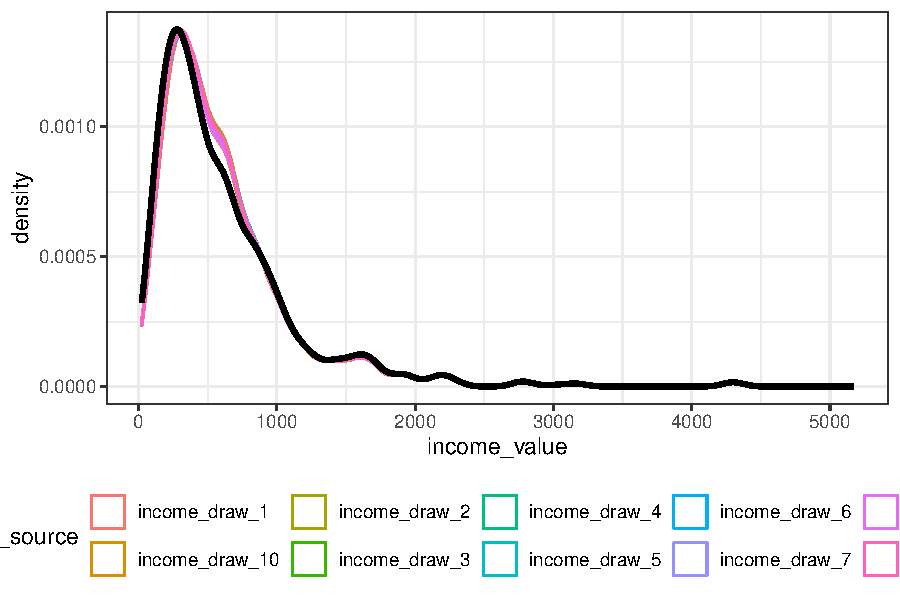
\includegraphics[width=0.7\linewidth,height=\textheight,keepaspectratio]{chapters/../figures/fig-ap3-imputation-multiple-1.pdf}

}

\caption{\label{fig-ap3-imputation-multiple}Distribución del ingreso
original y de los valores obtenidos mediante imputación múltiple}

\end{figure}%

Con los conjuntos de datos completados, el siguiente código
computacional define el diseño muestral que se utilizará para estimar
los parámetros de interés.

\begin{Shaded}
\begin{Highlighting}[]
\NormalTok{survey\_design }\OtherTok{\textless{}{-}}\NormalTok{ survey\_data }\SpecialCharTok{\%\textgreater{}\%}
  \FunctionTok{as\_survey\_design}\NormalTok{(}
    \AttributeTok{strata =}\NormalTok{ Stratum,}
    \AttributeTok{ids =}\NormalTok{ PSU,}
    \AttributeTok{weights =}\NormalTok{ wk,}
    \AttributeTok{nest =} \ConstantTok{TRUE}
\NormalTok{  )}
\end{Highlighting}
\end{Shaded}

A partir de este diseño, el siguiente código computacional estima la
media del ingreso y su varianza en cada conjunto de datos completado.

\begin{Shaded}
\begin{Highlighting}[]
\NormalTok{mean\_estimates }\OtherTok{\textless{}{-}}\NormalTok{ survey\_design }\SpecialCharTok{\%\textgreater{}\%}
  \FunctionTok{summarise}\NormalTok{(}
    \FunctionTok{across}\NormalTok{(}
      \FunctionTok{starts\_with}\NormalTok{(}\StringTok{"income\_draw\_"}\NormalTok{),}
      \SpecialCharTok{\textasciitilde{}} \FunctionTok{survey\_mean}\NormalTok{(.x, }\AttributeTok{vartype =} \StringTok{"var"}\NormalTok{)}
\NormalTok{    )}
\NormalTok{  ) }\SpecialCharTok{\%\textgreater{}\%}
\NormalTok{  tidyr}\SpecialCharTok{::}\FunctionTok{gather}\NormalTok{() }\SpecialCharTok{\%\textgreater{}\%}
  \FunctionTok{separate}\NormalTok{(}
\NormalTok{    key,}
    \FunctionTok{c}\NormalTok{(}\ConstantTok{NA}\NormalTok{, }\ConstantTok{NA}\NormalTok{, }\StringTok{"imputation"}\NormalTok{, }\StringTok{"statistic"}\NormalTok{),}
    \AttributeTok{fill =} \StringTok{"right"}
\NormalTok{  ) }\SpecialCharTok{\%\textgreater{}\%}
  \FunctionTok{mutate}\NormalTok{(}
    \AttributeTok{imputation =} \FunctionTok{as.numeric}\NormalTok{(imputation),}
    \AttributeTok{statistic =} \FunctionTok{ifelse}\NormalTok{(}\FunctionTok{is.na}\NormalTok{(statistic), }\StringTok{"mean"}\NormalTok{, }\StringTok{"var"}\NormalTok{)}
\NormalTok{  ) }\SpecialCharTok{\%\textgreater{}\%}
  \FunctionTok{spread}\NormalTok{(statistic, value)}

\NormalTok{mean\_estimates}
\end{Highlighting}
\end{Shaded}

\begin{verbatim}
# A tibble: 10 x 3
   imputation  mean   var
        <dbl> <dbl> <dbl>
 1          1  619.  846.
 2          2  618.  845.
 3          3  617.  868.
 4          4  618.  857.
 5          5  620.  858.
 6          6  617.  853.
 7          7  618.  861.
 8          8  619.  868.
 9          9  617.  850.
10         10  616.  870.
\end{verbatim}

El siguiente código computacional combina las medias estimadas y sus
varianzas mediante las reglas de imputación múltiple descritas
anteriormente.

\begin{Shaded}
\begin{Highlighting}[]
\NormalTok{pooled\_mean }\OtherTok{\textless{}{-}} \FunctionTok{mean}\NormalTok{(mean\_estimates}\SpecialCharTok{$}\NormalTok{mean)}
\NormalTok{within\_variance }\OtherTok{\textless{}{-}} \FunctionTok{mean}\NormalTok{(mean\_estimates}\SpecialCharTok{$}\NormalTok{var)}
\NormalTok{between\_variance }\OtherTok{\textless{}{-}} \FunctionTok{var}\NormalTok{(mean\_estimates}\SpecialCharTok{$}\NormalTok{mean)}

\NormalTok{within\_variance}
\end{Highlighting}
\end{Shaded}

\begin{verbatim}
[1] 857
\end{verbatim}

\begin{Shaded}
\begin{Highlighting}[]
\NormalTok{between\_variance}
\end{Highlighting}
\end{Shaded}

\begin{verbatim}
[1] 1.65
\end{verbatim}

\begin{Shaded}
\begin{Highlighting}[]
\NormalTok{pooled\_mean\_variance }\OtherTok{\textless{}{-}}\NormalTok{ within\_variance }\SpecialCharTok{+}
\NormalTok{  (}\DecValTok{1} \SpecialCharTok{+} \DecValTok{1} \SpecialCharTok{/}\NormalTok{ n\_imputations) }\SpecialCharTok{*}\NormalTok{ between\_variance}
\NormalTok{pooled\_results }\OtherTok{\textless{}{-}} \FunctionTok{data.frame}\NormalTok{(}
  \AttributeTok{pooled\_mean =}\NormalTok{ pooled\_mean,}
  \AttributeTok{mean\_se =} \FunctionTok{sqrt}\NormalTok{(pooled\_mean\_variance)}
\NormalTok{)}
\NormalTok{pooled\_results}
\end{Highlighting}
\end{Shaded}

\begin{verbatim}
  pooled_mean mean_se
1         618    29.3
\end{verbatim}

\begin{Shaded}
\begin{Highlighting}[]
\NormalTok{variance\_estimates }\OtherTok{\textless{}{-}}\NormalTok{ survey\_design }\SpecialCharTok{\%\textgreater{}\%}
  \FunctionTok{summarise\_at}\NormalTok{(}\FunctionTok{vars}\NormalTok{(}\FunctionTok{matches}\NormalTok{(}\StringTok{"income\_draw"}\NormalTok{)), survey\_var, }\AttributeTok{vartype =} \StringTok{"var"}\NormalTok{)}
\end{Highlighting}
\end{Shaded}

Otro parámetro de interés es la varianza del ingreso, que mide su
dispersión entre las personas de la muestra. Se sigue el mismo
procedimiento utilizado para la media: el siguiente código computacional
reorganiza las estimaciones de la varianza del ingreso y sus medidas de
incertidumbre para combinarlas por imputación.

\begin{Shaded}
\begin{Highlighting}[]
\NormalTok{variance\_estimates }\OtherTok{\textless{}{-}}\NormalTok{ variance\_estimates }\SpecialCharTok{\%\textgreater{}\%}
\NormalTok{  tidyr}\SpecialCharTok{::}\FunctionTok{gather}\NormalTok{() }\SpecialCharTok{\%\textgreater{}\%}
  \FunctionTok{separate}\NormalTok{(}
\NormalTok{    key,}
    \FunctionTok{c}\NormalTok{(}\ConstantTok{NA}\NormalTok{, }\ConstantTok{NA}\NormalTok{, }\StringTok{"imputation"}\NormalTok{, }\StringTok{"statistic"}\NormalTok{),}
    \AttributeTok{fill =} \StringTok{"right"}
\NormalTok{  ) }\SpecialCharTok{\%\textgreater{}\%}
  \FunctionTok{mutate}\NormalTok{(}
    \AttributeTok{statistic =} \FunctionTok{ifelse}\NormalTok{(}\FunctionTok{is.na}\NormalTok{(statistic), }\StringTok{"mean"}\NormalTok{, }\StringTok{"var"}\NormalTok{),}
    \AttributeTok{imputation =} \FunctionTok{as.numeric}\NormalTok{(imputation)}
\NormalTok{  ) }\SpecialCharTok{\%\textgreater{}\%}
  \FunctionTok{spread}\NormalTok{(statistic, value)}

\NormalTok{variance\_estimates}
\end{Highlighting}
\end{Shaded}

\begin{verbatim}
# A tibble: 10 x 3
   imputation    mean         var
        <dbl>   <dbl>       <dbl>
 1          1 262690. 3074674460.
 2          2 263092. 3079895581.
 3          3 274370. 3237991671.
 4          4 269127. 3164842634.
 5          5 270450. 3165285304.
 6          6 264993. 3106582542.
 7          7 270916. 3175865575.
 8          8 276070. 3251836316.
 9          9 265061. 3111426636.
10         10 275462. 3258214990.
\end{verbatim}

Por último, el siguiente código computacional combina las estimaciones
de la varianza del ingreso y su incertidumbre mediante las expresiones
anteriores.

\begin{Shaded}
\begin{Highlighting}[]
\NormalTok{pooled\_variance }\OtherTok{\textless{}{-}} \FunctionTok{mean}\NormalTok{(variance\_estimates}\SpecialCharTok{$}\NormalTok{mean)}
\NormalTok{within\_variance }\OtherTok{\textless{}{-}} \FunctionTok{mean}\NormalTok{(variance\_estimates}\SpecialCharTok{$}\NormalTok{var)}
\NormalTok{between\_variance }\OtherTok{\textless{}{-}} \FunctionTok{var}\NormalTok{(variance\_estimates}\SpecialCharTok{$}\NormalTok{mean)}
\NormalTok{pooled\_variance\_variance }\OtherTok{\textless{}{-}}\NormalTok{ within\_variance }\SpecialCharTok{+}
\NormalTok{  (}\DecValTok{1} \SpecialCharTok{+} \DecValTok{1} \SpecialCharTok{/}\NormalTok{ n\_imputations) }\SpecialCharTok{*}\NormalTok{ between\_variance}

\NormalTok{pooled\_results}\SpecialCharTok{$}\NormalTok{pooled\_variance }\OtherTok{\textless{}{-}}\NormalTok{ pooled\_variance}
\NormalTok{pooled\_results}\SpecialCharTok{$}\NormalTok{variance\_se }\OtherTok{\textless{}{-}} \FunctionTok{sqrt}\NormalTok{(pooled\_variance\_variance)}
\FunctionTok{cbind}\NormalTok{(pooled\_variance, pooled\_variance\_variance)}
\end{Highlighting}
\end{Shaded}

\begin{verbatim}
     pooled_variance pooled_variance_variance
[1,]          269223               3191037330
\end{verbatim}

\bookmarksetup{startatroot}

\chapter*{Referencias}\label{referencias}
\addcontentsline{toc}{chapter}{Referencias}

\markboth{Referencias}{Referencias}

\protect\phantomsection\label{refs}
\begin{CSLReferences}{1}{1}
\bibitem[\citeproctext]{ref-Agresti2019Intro}
Agresti, Alan. 2019. \emph{An Introduction to Categorical Data
Analysis}. 3.ª ed. John Wiley \& Sons.
\url{https://doi.org/10.1002/9781119405283}.

\bibitem[\citeproctext]{ref-Alexander1987}
Alexander, Charles H. 1987. {«A Class of Methods for Using Person
Controls in Household Weighting»}. \emph{Survey Methodology} 13 (2):
183-98.
\url{https://www150.statcan.gc.ca/n1/pub/12-001-x/1987002/article/14606-eng.pdf}.

\bibitem[\citeproctext]{ref-Anyanwu2014}
Anyanwu, John C. 2014. {«Marital Status, Household Size and Poverty in
{Nigeria}: Evidence from the 2009/2010 Survey Data»}. \emph{African
Development Review} 26 (1): 118-37.
\url{https://doi.org/10.1111/1467-8268.12069}.

\bibitem[\citeproctext]{ref-asparouhov2006general}
Asparouhov, Tihomir. 2006. {«General Multi-Level Modeling with Sampling
Weights»}. \emph{Communications in Statistics, Theory and Methods} 35
(3): 439-60. \url{https://doi.org/10.1080/03610920500476598}.

\bibitem[\citeproctext]{ref-pipe}
Bache, Stefan Milton, y Hadley Wickham. 2026. \emph{magrittr: A
Forward-Pipe Operator for R}.
\url{https://doi.org/10.32614/CRAN.package.magrittr}.

\bibitem[\citeproctext]{ref-BatesEtAl2015}
Bates, Douglas, Martin Mächler, Ben Bolker, y Steve Walker. 2015.
{«Fitting Linear Mixed-Effects Models Using lme4»}. \emph{Journal of
Statistical Software} 67 (1): 1-48.
\url{https://doi.org/10.18637/jss.v067.i01}.

\bibitem[\citeproctext]{ref-berglund2014multiple}
Berglund, Patricia, y Steven Heeringa. 2014. \emph{Multiple Imputation
of Missing Data Using {SAS}}. SAS Institute Inc.
\url{https://support.sas.com/content/dam/SAS/support/en/books/multiple-imputation-of-missing-data-using-sas/65370_excerpt.pdf}.

\bibitem[\citeproctext]{ref-binder1983variances}
Binder, David A. 1983. {«On the variances of asymptotically normal
estimators from complex surveys»}. \emph{International Statistical
Review/Revue Internationale de Statistique}, 279-92.

\bibitem[\citeproctext]{ref-binder2011estimating}
Binder, David A. 2011. {«Estimating model parameters from a complex
survey under a model-design randomization framework»}. \emph{Pakistan
Journal of Statistics} 27 (4).

\bibitem[\citeproctext]{ref-BinderKovacevic1995}
Binder, David A., y Milorad S. Kovačević. 1995. {«Estimating Some
Measures of Income Inequality from Survey Data: An Application of the
Estimating Equations Approach»}. \emph{Survey Methodology} 21 (2):
137-45.
\url{https://www150.statcan.gc.ca/n1/en/catalogue/12-001-X199500214396}.

\bibitem[\citeproctext]{ref-browne2006comparison}
Browne, William J., y David Draper. 2006. {«A Comparison of Bayesian and
Likelihood-Based Methods for Fitting Multilevel Models»}. \emph{Bayesian
Analysis} 1 (3): 473-514. \url{https://doi.org/10.1214/06-BA117}.

\bibitem[\citeproctext]{ref-bruch2011variance}
Bruch, Christian, Ralf Münnich, y Stefan Zins. 2011. {«Variance
estimation for complex surveys»}. \emph{Deliverable D3} 1.

\bibitem[\citeproctext]{ref-vanbuuren2012flexible}
Buuren, Stef van. 2012. \emph{Flexible Imputation of Missing Data}.
Chapman \& Hall/CRC. \url{https://doi.org/10.1201/b11826}.

\bibitem[\citeproctext]{ref-cai2013investigation}
Cai, Tianji. 2013. {«Investigation of Ways to Handle Sampling Weights
for Multilevel Model Analyses»}. \emph{Sociological Methodology} 43 (1):
178-219. \url{https://doi.org/10.1177/0081175013490035}.

\bibitem[\citeproctext]{ref-Carle2009}
Carle, Adam C. 2009. {«Fitting Multilevel Models in Complex Survey Data
with Design Weights: Recommendations»}. \emph{BMC Medical Research
Methodology} 9: 49. \url{https://doi.org/10.1186/1471-2288-9-49}.

\bibitem[\citeproctext]{ref-carpenter2013multiple}
Carpenter, James R., y Michael G. Kenward. 2013. \emph{Multiple
Imputation and its Application}. John Wiley \& Sons.
\url{https://doi.org/10.1002/9781119942283}.

\bibitem[\citeproctext]{ref-CasellaBerger2002}
Casella, George, y Roger L. Berger. 2002. \emph{Statistical Inference}.
2.ª ed. Duxbury.

\bibitem[\citeproctext]{ref-CEPAL2023Diseno}
CEPAL. 2023. \emph{Diseño y análisis estadístico de las encuestas de
hogares de América Latina}. Metodologías de la CEPAL 5. Naciones Unidas.
\url{https://repositorio.cepal.org/server/api/core/bitstreams/14d443ec-8f1e-44a7-b22b-9f124f205abe/content}.

\bibitem[\citeproctext]{ref-CEPAL2025PanoramaSocial}
CEPAL. 2025. \emph{Panorama Social de América Latina y el Caribe, 2025:
cómo salir de la trampa de alta desigualdad, baja movilidad social y
débil cohesión social}. {Comisión Económica para América Latina y el
Caribe}.
\url{https://repositorio.cepal.org/server/api/core/bitstreams/61e9dfa1-de2a-4af6-b670-0e2ed9b00cfe/content}.

\bibitem[\citeproctext]{ref-ChambersSkinner2003}
Chambers, Raymond L., y Chris J. Skinner, eds. 2003. \emph{Analysis of
Survey Data}. John Wiley \& Sons.
\url{https://doi.org/10.1002/0470867205}.

\bibitem[\citeproctext]{ref-cochran1977sampling}
Cochran, William Gemmell. 1977. \emph{Sampling techniques}. John Wiley
\& Sons.

\bibitem[\citeproctext]{ref-CEPAL2022PanoramaEnvejecimiento}
Comisión Económica para América Latina y el Caribe. 2022. {«Panorama del
envejecimiento y tendencias demográficas en América Latina y el
Caribe»}.
\url{https://www.cepal.org/es/enfoques/panorama-envejecimiento-tendencias-demograficas-america-latina-caribe}.

\bibitem[\citeproctext]{ref-Deaton1997}
Deaton, Angus. 1997. \emph{The Analysis of Household Surveys: A
Microeconometric Approach to Development Policy}. World Bank; The Johns
Hopkins University Press.

\bibitem[\citeproctext]{ref-DevilleSarndal1992}
Deville, Jean-Claude, y Carl-Erik Särndal. 1992. {«Calibration
Estimators in Survey Sampling»}. \emph{Journal of the American
Statistical Association} 87 (418): 376-82.
\url{https://doi.org/10.1080/01621459.1992.10475217}.

\bibitem[\citeproctext]{ref-DiazMoralesLeon2018}
Díaz Monroy, Luis Guillermo, Mario Alfonso Morales Rivera, y Leidy Rocío
León Dávila. 2018. \emph{Análisis estadístico de datos categóricos}. 1.ª
ed. Editorial Universidad Nacional de Colombia.
\url{https://portaldelibros.unal.edu.co/gpd-anyalisis-estadyustico-de-datos-categy-ricos-9789587834376-667e35367b60f.html}.

\bibitem[\citeproctext]{ref-DorfmanValliant1993}
Dorfman, Alan H., y Richard Valliant. 1993. {«Quantile Variance
Estimators in Complex Surveys»}. \emph{Proceedings of the Survey
Research Methods Section}, 866-71.

\bibitem[\citeproctext]{ref-efron1979bootstrap}
Efron, Bradley. 1979. {«Bootstrap methods: Another look at the
jackknife»}. \emph{The Annals of Statistics} 7 (1): 1-26.
\url{https://doi.org/10.1214/aos/1176344552}.

\bibitem[\citeproctext]{ref-FAO2026PoU}
FAO. 2026. \emph{Indicador 2.1.1: Prevalencia de la subalimentación}.
\url{https://www.fao.org/sustainable-development-goals-data-portal/data/indicators/2.1.1-prevalence-of-undernourishment/es}.

\bibitem[\citeproctext]{ref-fay1979contingency}
Fay, Robert E. 1979. {«On Adjusting the Pearson Chi-Square Statistic for
Cluster Sampling»}. \emph{Proceedings of the Social Statistics Section,
American Statistical Association}, 402-5.

\bibitem[\citeproctext]{ref-fellegi1980approximate}
Fellegi, Ivan P. 1980. {«Approximate Tests of Independence and Goodness
of Fit Based on Stratified Multistage Samples»}. \emph{Journal of the
American Statistical Association} 75 (370): 261-68.
\url{https://doi.org/10.2307/2287405}.

\bibitem[\citeproctext]{ref-Ferreira2026weightflow}
Ferreira, Juan Pablo. 2026. \emph{weightflow: Declarative API for Staged
Survey Weights}. \url{https://doi.org/10.32614/CRAN.package.weightflow}.

\bibitem[\citeproctext]{ref-finch2019multilevel}
Finch, W. Holmes, Jocelyn E. Bolin, y Ken Kelley. 2019. \emph{Multilevel
Modeling Using {R}}. 2.ª ed. CRC Press.

\bibitem[\citeproctext]{ref-FoxWeisberg2019}
Fox, John, y Sanford Weisberg. 2019. \emph{An R Companion to Applied
Regression}. 3.ª ed. SAGE Publications.

\bibitem[\citeproctext]{ref-FreedmanEllis2026}
Freedman Ellis, Greg, y Ben Schneider. 2026. \emph{srvyr: 'dplyr'-Like
Syntax for Summary Statistics of Survey Data}.
\url{https://doi.org/10.32614/CRAN.package.srvyr}.

\bibitem[\citeproctext]{ref-fuller1975regression}
Fuller, Wayne A. 1975. {«Regression analysis for sample survey»}.
\emph{Sankhya, Series C} 37: 117-32.

\bibitem[\citeproctext]{ref-fuller2002regression}
Fuller, Wayne A. 2002. {«Regression estimation for survey samples»}.
\emph{Survey Methodology} 28 (1): 5-23.

\bibitem[\citeproctext]{ref-Fuller2009}
Fuller, Wayne A. 2009. \emph{Sampling Statistics}. Wiley Series en
Survey Methodology. John Wiley \& Sons.
\url{https://doi.org/10.1002/9780470523551}.

\bibitem[\citeproctext]{ref-gambino2009sampling}
Gambino, Jack G, y Pedro Luis do Nascimento Silva. 2009. {«Sampling and
estimation in household surveys»}. En \emph{Handbook of Statistics},
vol. 29. Elsevier.

\bibitem[\citeproctext]{ref-gelman2006data}
Gelman, Andrew, y Jennifer Hill. 2006. \emph{Data Analysis Using
Regression and Multilevel/Hierarchical Models}. Cambridge University
Press.

\bibitem[\citeproctext]{ref-goldstein2011multilevel}
Goldstein, Harvey. 2011. \emph{Multilevel Statistical Models}. 4.ª ed.
John Wiley \& Sons.

\bibitem[\citeproctext]{ref-Groves2009}
Groves, Robert M., Floyd J. Fowler, Mick P. Couper, James M. Lepkowski,
Eleanor Singer, y Roger Tourangeau. 2009. \emph{Survey Methodology}. 2.ª
ed. John Wiley \& Sons.

\bibitem[\citeproctext]{ref-Gutierrez2016}
Gutiérrez, Andrés. 2016. \emph{Estrategias de muestreo: diseño de
encuestas y estimación de parámetros}. Segunda edición. Ediciones de la
U.

\bibitem[\citeproctext]{ref-GutierrezT2020}
Gutiérrez, Andrés. 2020. \emph{TeachingSampling: Selection of Samples
and Parameter Estimation in Finite Population}.
\url{https://doi.org/10.32614/CRAN.package.TeachingSampling}.

\bibitem[\citeproctext]{ref-GutierrezBabativa2023}
Gutiérrez, Andrés, y Giovany Babativa-Márquez. 2023. \emph{Efectos de
diseño para indicadores sociales en Am{é}rica Latina: función
generalizada de varianza para estimadores directos provenientes de
encuestas de hogares}. LC/TS.2023/95 No. 106. CEPAL - Serie Estudios
Estadísticos. CEPAL.
\url{https://repositorio.cepal.org/server/api/core/bitstreams/feb8c8be-6434-41f2-8fd9-f12f71a0739a/content}.

\bibitem[\citeproctext]{ref-hansen1953sample}
{Hansen, Morris H, William N Hurwitz, William G Madow, et~al.} 1953.
\emph{Sample survey methods and theory}.

\bibitem[\citeproctext]{ref-HeeringaWestBerglund2017}
Heeringa, Steven G., Brady T. West, y Patricia A. Berglund. 2017.
\emph{Applied Survey Data Analysis}. 2.ª ed. Chapman \& Hall/CRC.
\url{https://doi.org/10.1201/9781315153278}.

\bibitem[\citeproctext]{ref-ggstance2024}
Henry, Lionel, Hadley Wickham, y Winston Chang. 2024. \emph{ggstance:
Horizontal 'ggplot2' Components}.
\url{https://doi.org/10.32614/CRAN.package.ggstance}.

\bibitem[\citeproctext]{ref-HorvitzThompson1952}
Horvitz, Daniel G., y Donovan J. Thompson. 1952. {«A Generalization of
Sampling Without Replacement from a Finite Universe»}. \emph{Journal of
the American Statistical Association} 47 (260): 663-85.
\url{https://doi.org/10.1080/01621459.1952.10483446}.

\bibitem[\citeproctext]{ref-convey2024}
Jacob, Guilherme, Djalma Pessoa, y Anthony Damico. 2024. \emph{convey:
Income Concentration Analysis with Complex Survey Samples}.
\url{https://doi.org/10.32614/CRAN.package.convey}.

\bibitem[\citeproctext]{ref-kalton2003weighting}
Kalton, Graham, y Ismael Flores-Cervantes. 2003. {«Weighting methods»}.
\emph{Journal of official statistics} 19 (2): 81.

\bibitem[\citeproctext]{ref-kim2004fractional}
Kim, Jae Kwang, y Wayne Fuller. 2004. {«Fractional Hot Deck
Imputation»}. \emph{Biometrika} 91 (3): 559-78.
\url{https://doi.org/10.1093/biomet/91.3.559}.

\bibitem[\citeproctext]{ref-kim2014statistical}
Kim, Jae Kwang, y Jun Shao. 2014. \emph{Statistical Methods for Handling
Incomplete Data}. Chapman \& Hall/CRC.

\bibitem[\citeproctext]{ref-kish1965survey}
Kish, Leslie. 1965. \emph{Survey Sampling}. Wiley.

\bibitem[\citeproctext]{ref-kish1974inference}
Kish, Leslie, y Martin R. Frankel. 1974. {«Inference from complex
samples»}. \emph{Journal of the Royal Statistical Society, Series B} 36:
1-37.

\bibitem[\citeproctext]{ref-KornGraubard1999}
Korn, Edward L., y Barry I. Graubard. 1999. \emph{Analysis of Health
Surveys}. John Wiley \& Sons.
\url{https://doi.org/10.1002/9781118032619}.

\bibitem[\citeproctext]{ref-korn1995analysis}
Korn, Edward L, y Barry I Graubard. 1995. {«Analysis of large health
surveys: accounting for the sampling design»}. \emph{Journal of the
Royal Statistical Society: Series A (Statistics in Society)} 158 (2):
263-95.

\bibitem[\citeproctext]{ref-KovacevicBinder1997}
Kovačević, Milorad S., y David A. Binder. 1997. {«Variance Estimation
for Measures of Income Inequality and Polarization: The Estimating
Equations Approach»}. \emph{Journal of Official Statistics} 13 (1):
41-58.

\bibitem[\citeproctext]{ref-kovar1988}
Kovar, JG, JNK Rao, y CFJ Wu. 1988. {«Bootstrap and other methods to
measure errors in survey estimates»}. \emph{Canadian Journal of
Statistics} 16 (S1): 25-45.

\bibitem[\citeproctext]{ref-LangelTille2013}
Langel, Matti, y Yves Tillé. 2013. {«Variance Estimation of the Gini
Index: Revisiting a Result Several Times Published»}. \emph{Journal of
the Royal Statistical Society: Series A (Statistics in Society)} 176
(2): 521-40. \url{https://doi.org/10.1111/j.1467-985X.2012.01048.x}.

\bibitem[\citeproctext]{ref-Li_Valliant_2015}
Li, Jianzhu, y Richard Valliant. 2015. {«Linear Regression Diagnostics
in Cluster Samples»}. \emph{Journal of Official Statistics} 31 (1):
61-75. \url{https://doi.org/10.1515/jos-2015-0003}.

\bibitem[\citeproctext]{ref-jtools2026}
Long, Jacob A. 2026. \emph{jtools: Analysis and Presentation of Social
Scientific Data}. \url{https://doi.org/10.32614/CRAN.package.jtools}.

\bibitem[\citeproctext]{ref-Lorenz1905}
Lorenz, Max O. 1905. {«Methods of Measuring the Concentration of
Wealth»}. \emph{Publications of the American Statistical Association} 9
(70): 209-19. \url{https://doi.org/10.2307/2276207}.

\bibitem[\citeproctext]{ref-performance2026}
Lüdecke, Daniel, Mattan S. Ben-Shachar, Indrajeet Patil, Philip
Waggoner, y Dominique Makowski. 2026. \emph{performance: Assessment of
Regression Models Performance}.
\url{https://doi.org/10.32614/CRAN.package.performance}.

\bibitem[\citeproctext]{ref-Lumley2010}
Lumley, Thomas. 2010. \emph{Complex Surveys: A Guide to Analysis Using
R: A Guide to Analysis Using R}. John Wiley \& Sons.

\bibitem[\citeproctext]{ref-svyVGAM2026}
Lumley, Thomas. 2026. \emph{svyVGAM: Design-Based Inference in Vector
Generalised Linear Models}.
\url{https://doi.org/10.32614/CRAN.package.svyVGAM}.

\bibitem[\citeproctext]{ref-Lumley2026}
Lumley, Thomas, Peter Gao, Ben Schneider, y Stas Kolenikov. 2026.
\emph{survey: Analysis of Complex Survey Samples}.
\url{https://doi.org/10.32614/CRAN.package.survey}.

\bibitem[\citeproctext]{ref-McCullaghNelder1989}
McCullagh, Peter, y John A. Nelder. 1989. \emph{Generalized Linear
Models}. 2.ª ed. Chapman \& Hall.
\url{https://doi.org/10.1007/978-1-4899-3242-6}.

\bibitem[\citeproctext]{ref-merlo2006brief}
Merlo, Juan, Basile Chaix, Henrik Ohlsson, et~al. 2006. {«A Brief
Conceptual Tutorial of Multilevel Analysis in Social Epidemiology: Using
Measures of Clustering in Multilevel Logistic Regression to Investigate
Contextual Phenomena»}. \emph{Journal of Epidemiology \& Community
Health} 60 (4): 290-97. \url{https://doi.org/10.1136/jech.2004.029454}.

\bibitem[\citeproctext]{ref-molina1992pseudo}
Molina, Elizabeth A., y Chris J. Skinner. 1992. {«Pseudo-likelihood and
quasi-likelihood estimation for complex sampling schemes»}.
\emph{Computational Statistics \& Data Analysis} 13: 395-405.

\bibitem[\citeproctext]{ref-UnitedNations2005}
Naciones Unidas. 2005. \emph{Designing Household Survey Samples:
Practical Guidelines}. Studies en Methods, Series F, No. 98. United
Nations.

\bibitem[\citeproctext]{ref-ONUDeff}
Naciones Unidas. 2009. \emph{Diseño de Muestras para Encuestas de
Hogares: Directrices Prácticas.} Estudios de Métodos, Serie F 98.
Naciones Unidas.
\url{https://unstats.un.org/unsd/publication/seriesf/seriesf_98s.pdf}.

\bibitem[\citeproctext]{ref-unitednations2021householdsurveys}
Naciones Unidas. 2021. \emph{Report of the Intersecretariat Working
Group on Household Surveys}. E/CN.3/2021/16. United Nations Statistical
Commission.

\bibitem[\citeproctext]{ref-UNhandbook}
Naciones Unidas. 2026. \emph{Handbook of Surveys on Households and
Individuals Foundations and Emerging Approaches}. Naciones Unidas.

\bibitem[\citeproctext]{ref-nelder1972generalized}
Nelder, John A., y Robert W. M. Wedderburn. 1972. {«Generalized Linear
Models»}. \emph{Journal of the Royal Statistical Society: Series A
(General)} 135 (3): 370-84. \url{https://doi.org/10.2307/2344614}.

\bibitem[\citeproctext]{ref-OECD2013ICW}
OECD. 2013. \emph{OECD Framework for Statistics on the Distribution of
Household Income, Consumption and Wealth}. OECD Publishing.
\url{https://doi.org/10.1787/9789264194830-en}.

\bibitem[\citeproctext]{ref-osier2009variance}
Osier, Guillaume. 2009. {«Variance estimation for complex indicators of
poverty and inequality using linearization techniques»}. \emph{Survey
research methods} 3: 167-95.

\bibitem[\citeproctext]{ref-Park2003Design}
Park, Inho, Marianne Winglee, Jay Clark, Keith Rust, Andrea Sedlak, y
David Morganstein. 2003. {«Design Effects and Survey Planning»}.
\emph{Proceedings of the Section on Survey Research Methods}, 3179-86.
\url{https://www.asasrms.org/Proceedings/y2003/Files/JSM2003-000156.pdf}.

\bibitem[\citeproctext]{ref-Pebesma2018sf}
Pebesma, Edzer. 2018. {«Simple Features for R: Standardized Support for
Spatial Vector Data»}. \emph{The R Journal} 10 (1): 439-46.
\url{https://doi.org/10.32614/RJ-2018-009}.

\bibitem[\citeproctext]{ref-sf2026}
Pebesma, Edzer, Roger Bivand, Etienne Racine, et~al. 2026. \emph{sf:
Simple Features for R}. \url{https://doi.org/10.32614/CRAN.package.sf}.

\bibitem[\citeproctext]{ref-patchwork}
Pedersen, Thomas Lin. 2025. \emph{patchwork: The composer of plots}.
\url{https://doi.org/10.32614/CRAN.package.patchwork}.

\bibitem[\citeproctext]{ref-pfeffermann1993role}
Pfeffermann, Danny. 1993. {«The Role of Sampling Weights When Modeling
Survey Data»}. \emph{International Statistical Review} 61 (2): 317-37.
\url{https://doi.org/10.2307/1403631}.

\bibitem[\citeproctext]{ref-pfeffermann2011modelling}
Pfeffermann, Danny. 2011. {«Modelling of complex survey data: {W}hy
model? {W}hy is it a problem? {H}ow can we approach it?»} \emph{Survey
Methodology} 37 (2): 115-36.

\bibitem[\citeproctext]{ref-pfeffermann1998weighting}
Pfeffermann, Danny, Chris J. Skinner, David J. Holmes, Harvey Goldstein,
y Jon Rasbash. 1998. {«Weighting for Unequal Selection Probabilities in
Multilevel Models»}. \emph{Journal of the Royal Statistical Society:
Series B} 60 (1): 23-40. \url{https://doi.org/10.1111/1467-9868.00106}.

\bibitem[\citeproctext]{ref-PositProjects2026}
Posit Software, PBC. 2026. \emph{RStudio Projects}. Posit Software, PBC.
\url{https://docs.posit.co/ide/user/ide/guide/code/projects.html}.

\bibitem[\citeproctext]{ref-biscale2025}
Prener, Christopher, Timo Grossenbacher, y Angelo Zehr. 2025.
\emph{biscale: Tools and Palettes for Bivariate Thematic Mapping}.
\url{https://doi.org/10.32614/CRAN.package.biscale}.

\bibitem[\citeproctext]{ref-RCoreTeam2026}
R Core Team. 2026a. \emph{R: A Language and Environment for Statistical
Computing}. R Foundation for Statistical Computing.
\url{https://www.R-project.org/}.

\bibitem[\citeproctext]{ref-RCoreSerialization2026}
R Core Team. 2026b. \emph{Serialization Interface for Single Objects}. R
Foundation for Statistical Computing.
\url{https://stat.ethz.ch/R-manual/R-devel/library/base/html/readRDS.html}.

\bibitem[\citeproctext]{ref-rabehesketh2006multilevel}
Rabe-Hesketh, Sophia, y Anders Skrondal. 2006. {«Multilevel Modelling of
Complex Survey Data»}. \emph{Journal of the Royal Statistical Society:
Series A} 169 (4): 805-27.
\url{https://doi.org/10.1111/j.1467-985X.2006.00426.x}.

\bibitem[\citeproctext]{ref-rabehesketh2012multilevel}
Rabe-Hesketh, Sophia, y Anders Skrondal. 2012. \emph{Multilevel and
Longitudinal Modeling Using Stata}. 3.ª ed. Stata Press.

\bibitem[\citeproctext]{ref-raghunathan2016missing}
Raghunathan, Trivellore. 2016. \emph{Missing Data Analysis in Practice}.
Chapman \& Hall/CRC.
\url{https://www.routledge.com/Missing-Data-Analysis-in-Practice/Raghunathan/p/book/9780429171673}.

\bibitem[\citeproctext]{ref-RaoMolina2015}
Rao, J. N. K., y Isabel Molina. 2015. \emph{Small Area Estimation}. 2.ª
ed. John Wiley \& Sons. \url{https://doi.org/10.1002/9781118735855}.

\bibitem[\citeproctext]{ref-RaoScott1981}
Rao, J. N. K., y Alastair J. Scott. 1981. {«The Analysis of Categorical
Data From Complex Sample Surveys: Chi-Squared Tests for Goodness of Fit
and Independence in Two-Way Tables»}. \emph{Journal of the American
Statistical Association} 76 (374): 221-30.
\url{https://doi.org/10.1080/01621459.1981.10477633}.

\bibitem[\citeproctext]{ref-rao1992resampling}
Rao, J. N. K., C. F. J. Wu, y K. Yue. 1992. {«Some recent work on
resampling methods for complex surveys»}. \emph{Survey Methodology} 18:
209-17.

\bibitem[\citeproctext]{ref-rao1984chisquare}
Rao, Jon N. K., y Alastair J. Scott. 1984. {«On chi-squared tests for
multiway contingency tables with cell proportions estimated from survey
data»}. \emph{The Annals of Statistics} 12 (1): 46-60.

\bibitem[\citeproctext]{ref-rubin1987multiple}
Rubin, Donald B. 1987. \emph{Multiple Imputation for Nonresponse in
Surveys}. Wiley Series en Probability y Statistics. John Wiley \& Sons.
\url{https://doi.org/10.1002/9780470316696}.

\bibitem[\citeproctext]{ref-RustRao1996}
Rust, Keith F., y J. N. K. Rao. 1996. {«Variance Estimation for Complex
Surveys Using Replication Techniques»}. \emph{Statistical Methods in
Medical Research} 5 (3): 283-310.
\url{https://doi.org/10.1177/096228029600500305}.

\bibitem[\citeproctext]{ref-sarndal2005nonresponse}
Särndal, Carl-Erik, y Sixten Lundström. 2005. \emph{Estimation in
surveys with nonresponse}. John Wiley \& Sons.

\bibitem[\citeproctext]{ref-sarndal2003model}
Särndal, Carl-Erik, Bengt Swensson, y Jan Wretman. 2003. \emph{Model
assisted survey sampling}. Springer Science \& Business Media.

\bibitem[\citeproctext]{ref-SAS2012StdDev}
SAS Institute Inc. 2012. \emph{Estimating the Standard Deviation of a
Variable in a Finite Population}. SAS Support, Sample 45701.
\url{https://support.sas.com/kb/45/701.html}.

\bibitem[\citeproctext]{ref-SchulzeWaltrupKauermann2016}
Schulze Waltrup, Linda, y Göran Kauermann. 2016. {«A Short Note on
Quantile and Expectile Estimation in Unequal Probability Samples»}.
\emph{Survey Methodology} 42 (1): 179-87.
\url{https://www150.statcan.gc.ca/n1/en/catalogue/12-001-X201600114545}.

\bibitem[\citeproctext]{ref-shah1977inference}
Shah, Babubhai V., Maurice M. Holt, y Ralph F. Folsom. 1977. {«Inference
about regression models from sample survey data»}. \emph{Bulletin of the
International Statistical Institute} 41 (3): 43-57.

\bibitem[\citeproctext]{ref-skinner1989analysis}
Skinner, Chris J., David Holt, y Tom M. F. Smith, eds. 1989.
\emph{Analysis of complex surveys}. John Wiley \& Sons.

\bibitem[\citeproctext]{ref-snijders2011}
Snijders, Tom AB, y Roel Bosker. 2011. \emph{Multilevel analysis: An
introduction to basic and advanced multilevel modeling}.

\bibitem[\citeproctext]{ref-dotwhisker2025}
Solt, Frederick, y Yue Hu. 2025. \emph{dotwhisker: Dot-and-Whisker Plots
of Regression Results}.
\url{https://doi.org/10.32614/CRAN.package.dotwhisker}.

\bibitem[\citeproctext]{ref-Tennekes2018tmap}
Tennekes, Martijn. 2018. {«tmap: Thematic Maps in R»}. \emph{Journal of
Statistical Software} 84 (6): 1-39.
\url{https://doi.org/10.18637/jss.v084.i06}.

\bibitem[\citeproctext]{ref-tmap2026}
Tennekes, Martijn. 2026. \emph{tmap: Thematic Maps}.
\url{https://doi.org/10.32614/CRAN.package.tmap}.

\bibitem[\citeproctext]{ref-thomas1987chisquare}
Thomas, D. Roland, y Jon N. K. Rao. 1987. {«Small-sample comparisons of
level and power for simple goodness-of-fit statistics under cluster
sampling»}. \emph{Journal of the American Statistical Association} 82
(398): 630-36.

\bibitem[\citeproctext]{ref-TilleMatei2025}
Tillé, Yves, y Alina Matei. 2025. \emph{sampling: Survey Sampling}.
\url{https://doi.org/10.32614/CRAN.package.sampling}.

\bibitem[\citeproctext]{ref-Tukey1977EDA}
Tukey, John W. 1977. \emph{Exploratory Data Analysis}. Addison-Wesley.

\bibitem[\citeproctext]{ref-UNECE2011Canberra}
UNECE. 2011. \emph{Canberra Group Handbook on Household Income
Statistics}. 2.ª ed. {United Nations Economic Commission for Europe}.

\bibitem[\citeproctext]{ref-Valliant2024}
Valliant, Richard. 2024. \emph{svydiags: Regression Model Diagnostics
for Survey Data}. \url{https://doi.org/10.32614/CRAN.package.svydiags}.

\bibitem[\citeproctext]{ref-Valliant_Dever_2017}
Valliant, Richard, y Jill A. Dever. 2017. \emph{Survey Weights: A
Step-by-step Guide to Calculation}. 1 edition. Stata Press.

\bibitem[\citeproctext]{ref-Valliant_Dever_Kreuter_2018}
Valliant, Richard, Jill A. Dever, y Frauke Kreuter. 2018.
\emph{Practical Tools for Designing and Weighting Survey Samples}.
Statistics for Social y Behavioral Sciences. Springer International
Publishing. \url{https://doi.org/10.1007/978-3-319-93632-1}.

\bibitem[\citeproctext]{ref-gtools2025}
Warnes, Gregory R., Ben Bolker, Thomas Lumley, et~al. 2023.
\emph{gtools: Various R Programming Tools}.
\url{https://doi.org/10.32614/CRAN.package.gtools}.

\bibitem[\citeproctext]{ref-Wickham2014}
Wickham, Hadley. 2014. {«Tidy Data»}. \emph{Journal of Statistical
Software} 59 (10): 1-23. \url{https://doi.org/10.18637/jss.v059.i10}.

\bibitem[\citeproctext]{ref-tidyverse2026}
Wickham, Hadley, Mara Averick, Jennifer Bryan, et~al. 2026.
\emph{tidyverse: Easily Install and Load the Tidyverse}.
\url{https://doi.org/10.32614/CRAN.package.tidyverse}.

\bibitem[\citeproctext]{ref-WickhamEtAl2023}
Wickham, Hadley, Mine Çetinkaya-Rundel, y Garrett Grolemund. 2023.
\emph{R for Data Science: Import, Tidy, Transform, Visualize, and Model
Data}. 2.ª ed. O'Reilly Media. \url{https://r4ds.hadley.nz/}.

\bibitem[\citeproctext]{ref-ggplot22026}
Wickham, Hadley, Winston Chang, Lionel Henry, et~al. 2026.
\emph{ggplot2: Create Elegant Data Visualisations Using the Grammar of
Graphics}. \url{https://doi.org/10.32614/CRAN.package.ggplot2}.

\bibitem[\citeproctext]{ref-dplyr2026}
Wickham, Hadley, Romain François, Lionel Henry, Kirill Müller, y Davis
Vaughan. 2026. \emph{dplyr: A Grammar of Data Manipulation}.
\url{https://doi.org/10.32614/CRAN.package.dplyr}.

\bibitem[\citeproctext]{ref-cowplot2025}
Wilke, Claus O. 2025. \emph{cowplot: Streamlined Plot Theme and Plot
Annotations for 'ggplot2'}.
\url{https://doi.org/10.32614/CRAN.package.cowplot}.

\bibitem[\citeproctext]{ref-wilkinson2005grammar}
Wilkinson, Leland. 2005. \emph{The grammar of graphics}. 2.ª ed.
Springer.

\bibitem[\citeproctext]{ref-Wolter2007Variance}
Wolter, Kirk M. 2007. \emph{Introduction to Variance Estimation}. 2.ª
ed. Springer Series en Statistics. Springer.
\url{https://doi.org/10.1007/978-0-387-35099-8}.

\bibitem[\citeproctext]{ref-Woodruff1952}
Woodruff, Ralph S. 1952. {«Confidence Intervals for Medians and Other
Position Measures»}. \emph{Journal of the American Statistical
Association} 47 (260): 635-46.
\url{https://doi.org/10.1080/01621459.1952.10483443}.

\bibitem[\citeproctext]{ref-woodruff1971simple}
Woodruff, Ralph S. 1971. {«A Simple Method for Approximating the
Variance of a Complicated Estimate»}. \emph{Journal of the American
Statistical Association} 66 (334): 411-14.
\url{https://doi.org/10.1080/01621459.1971.10482279}.

\bibitem[\citeproctext]{ref-Wooldridge2020}
Wooldridge, Jeffrey M. 2020. \emph{Introductory Econometrics: A Modern
Approach}. 7.ª ed. Cengage Learning.
\url{https://www.cengage.com/c/introductory-econometrics-a-modern-approach-7e-wooldridge/9781337558860}.

\end{CSLReferences}


\backmatter


\end{document}
